\documentclass[]{book}
\usepackage{lmodern}
\usepackage{amssymb,amsmath}
\usepackage{ifxetex,ifluatex}
\usepackage{fixltx2e} % provides \textsubscript
\ifnum 0\ifxetex 1\fi\ifluatex 1\fi=0 % if pdftex
  \usepackage[T1]{fontenc}
  \usepackage[utf8]{inputenc}
\else % if luatex or xelatex
  \ifxetex
    \usepackage{mathspec}
  \else
    \usepackage{fontspec}
  \fi
  \defaultfontfeatures{Ligatures=TeX,Scale=MatchLowercase}
\fi
% use upquote if available, for straight quotes in verbatim environments
\IfFileExists{upquote.sty}{\usepackage{upquote}}{}
% use microtype if available
\IfFileExists{microtype.sty}{%
\usepackage[]{microtype}
\UseMicrotypeSet[protrusion]{basicmath} % disable protrusion for tt fonts
}{}
\PassOptionsToPackage{hyphens}{url} % url is loaded by hyperref
\usepackage[unicode=true]{hyperref}
\hypersetup{
            pdftitle={Statistics for Data Science Notes},
            pdfauthor={Andrew Sage - Stat 255: Lawrence University},
            pdfborder={0 0 0},
            breaklinks=true}
\urlstyle{same}  % don't use monospace font for urls
\usepackage{natbib}
\bibliographystyle{plainnat}
\usepackage{color}
\usepackage{fancyvrb}
\newcommand{\VerbBar}{|}
\newcommand{\VERB}{\Verb[commandchars=\\\{\}]}
\DefineVerbatimEnvironment{Highlighting}{Verbatim}{commandchars=\\\{\}}
% Add ',fontsize=\small' for more characters per line
\usepackage{framed}
\definecolor{shadecolor}{RGB}{248,248,248}
\newenvironment{Shaded}{\begin{snugshade}}{\end{snugshade}}
\newcommand{\KeywordTok}[1]{\textcolor[rgb]{0.13,0.29,0.53}{\textbf{#1}}}
\newcommand{\DataTypeTok}[1]{\textcolor[rgb]{0.13,0.29,0.53}{#1}}
\newcommand{\DecValTok}[1]{\textcolor[rgb]{0.00,0.00,0.81}{#1}}
\newcommand{\BaseNTok}[1]{\textcolor[rgb]{0.00,0.00,0.81}{#1}}
\newcommand{\FloatTok}[1]{\textcolor[rgb]{0.00,0.00,0.81}{#1}}
\newcommand{\ConstantTok}[1]{\textcolor[rgb]{0.00,0.00,0.00}{#1}}
\newcommand{\CharTok}[1]{\textcolor[rgb]{0.31,0.60,0.02}{#1}}
\newcommand{\SpecialCharTok}[1]{\textcolor[rgb]{0.00,0.00,0.00}{#1}}
\newcommand{\StringTok}[1]{\textcolor[rgb]{0.31,0.60,0.02}{#1}}
\newcommand{\VerbatimStringTok}[1]{\textcolor[rgb]{0.31,0.60,0.02}{#1}}
\newcommand{\SpecialStringTok}[1]{\textcolor[rgb]{0.31,0.60,0.02}{#1}}
\newcommand{\ImportTok}[1]{#1}
\newcommand{\CommentTok}[1]{\textcolor[rgb]{0.56,0.35,0.01}{\textit{#1}}}
\newcommand{\DocumentationTok}[1]{\textcolor[rgb]{0.56,0.35,0.01}{\textbf{\textit{#1}}}}
\newcommand{\AnnotationTok}[1]{\textcolor[rgb]{0.56,0.35,0.01}{\textbf{\textit{#1}}}}
\newcommand{\CommentVarTok}[1]{\textcolor[rgb]{0.56,0.35,0.01}{\textbf{\textit{#1}}}}
\newcommand{\OtherTok}[1]{\textcolor[rgb]{0.56,0.35,0.01}{#1}}
\newcommand{\FunctionTok}[1]{\textcolor[rgb]{0.00,0.00,0.00}{#1}}
\newcommand{\VariableTok}[1]{\textcolor[rgb]{0.00,0.00,0.00}{#1}}
\newcommand{\ControlFlowTok}[1]{\textcolor[rgb]{0.13,0.29,0.53}{\textbf{#1}}}
\newcommand{\OperatorTok}[1]{\textcolor[rgb]{0.81,0.36,0.00}{\textbf{#1}}}
\newcommand{\BuiltInTok}[1]{#1}
\newcommand{\ExtensionTok}[1]{#1}
\newcommand{\PreprocessorTok}[1]{\textcolor[rgb]{0.56,0.35,0.01}{\textit{#1}}}
\newcommand{\AttributeTok}[1]{\textcolor[rgb]{0.77,0.63,0.00}{#1}}
\newcommand{\RegionMarkerTok}[1]{#1}
\newcommand{\InformationTok}[1]{\textcolor[rgb]{0.56,0.35,0.01}{\textbf{\textit{#1}}}}
\newcommand{\WarningTok}[1]{\textcolor[rgb]{0.56,0.35,0.01}{\textbf{\textit{#1}}}}
\newcommand{\AlertTok}[1]{\textcolor[rgb]{0.94,0.16,0.16}{#1}}
\newcommand{\ErrorTok}[1]{\textcolor[rgb]{0.64,0.00,0.00}{\textbf{#1}}}
\newcommand{\NormalTok}[1]{#1}
\usepackage{longtable,booktabs}
% Fix footnotes in tables (requires footnote package)
\IfFileExists{footnote.sty}{\usepackage{footnote}\makesavenoteenv{long table}}{}
\usepackage{graphicx,grffile}
\makeatletter
\def\maxwidth{\ifdim\Gin@nat@width>\linewidth\linewidth\else\Gin@nat@width\fi}
\def\maxheight{\ifdim\Gin@nat@height>\textheight\textheight\else\Gin@nat@height\fi}
\makeatother
% Scale images if necessary, so that they will not overflow the page
% margins by default, and it is still possible to overwrite the defaults
% using explicit options in \includegraphics[width, height, ...]{}
\setkeys{Gin}{width=\maxwidth,height=\maxheight,keepaspectratio}
\IfFileExists{parskip.sty}{%
\usepackage{parskip}
}{% else
\setlength{\parindent}{0pt}
\setlength{\parskip}{6pt plus 2pt minus 1pt}
}
\setlength{\emergencystretch}{3em}  % prevent overfull lines
\providecommand{\tightlist}{%
  \setlength{\itemsep}{0pt}\setlength{\parskip}{0pt}}
\setcounter{secnumdepth}{5}
% Redefines (sub)paragraphs to behave more like sections
\ifx\paragraph\undefined\else
\let\oldparagraph\paragraph
\renewcommand{\paragraph}[1]{\oldparagraph{#1}\mbox{}}
\fi
\ifx\subparagraph\undefined\else
\let\oldsubparagraph\subparagraph
\renewcommand{\subparagraph}[1]{\oldsubparagraph{#1}\mbox{}}
\fi

% set default figure placement to htbp
\makeatletter
\def\fps@figure{htbp}
\makeatother

\usepackage{booktabs}

\title{Statistics for Data Science Notes}
\author{Andrew Sage - Stat 255: Lawrence University}
\date{2021-09-25}

\begin{document}
\maketitle

{
\setcounter{tocdepth}{1}
\tableofcontents
}
\chapter{Exploratory Data Analysis}\label{exploratory-data-analysis}

\section{Exploring Diamond Prices}\label{exploring-diamond-prices}

We consider a dataset with prices (in \$ US) and other information on
53,940 round cut diamonds. The first 6 rows are shown below.

\begin{Shaded}
\begin{Highlighting}[]
\KeywordTok{library}\NormalTok{(tidyverse)}
\KeywordTok{data}\NormalTok{(diamonds)}
\KeywordTok{head}\NormalTok{(diamonds)}
\end{Highlighting}
\end{Shaded}

\begin{verbatim}
##   carat       cut color clarity depth table price    x    y    z
## 1  0.23     Ideal     E     SI2  61.5    55   326 3.95 3.98 2.43
## 2  0.21   Premium     E     SI1  59.8    61   326 3.89 3.84 2.31
## 3  0.23      Good     E     VS1  56.9    65   327 4.05 4.07 2.31
## 4  0.29   Premium     I     VS2  62.4    58   334 4.20 4.23 2.63
## 5  0.31      Good     J     SI2  63.3    58   335 4.34 4.35 2.75
## 6  0.24 Very Good     J    VVS2  62.8    57   336 3.94 3.96 2.48
\end{verbatim}

The dataset incudes both:

\begin{itemize}
\tightlist
\item
  \textbf{categorical} (or factor) variables cut, color, clarity, and\\
\item
  \textbf{quantitative} (or numeric) variables, depth, table, price, x,
  y, z
\end{itemize}

\subsection{Boxplot of Diamond Prices}\label{boxplot-of-diamond-prices}

\begin{Shaded}
\begin{Highlighting}[]
\KeywordTok{ggplot}\NormalTok{(}\DataTypeTok{data=}\NormalTok{diamonds, }\KeywordTok{aes}\NormalTok{(}\DataTypeTok{x=}\NormalTok{price, }\DataTypeTok{y=}\NormalTok{cut, }\DataTypeTok{fill=}\NormalTok{cut)) }\OperatorTok{+}\StringTok{ }
\StringTok{  }\KeywordTok{geom_boxplot}\NormalTok{(}\DataTypeTok{outlier.size=}\FloatTok{0.01}\NormalTok{, }\DataTypeTok{outlier.alpha =} \FloatTok{0.1}\NormalTok{) }\OperatorTok{+}\StringTok{ }
\StringTok{    }\KeywordTok{stat_summary}\NormalTok{(}\DataTypeTok{fun=}\NormalTok{mean, }\DataTypeTok{geom=}\StringTok{"point"}\NormalTok{, }\DataTypeTok{shape=}\DecValTok{4}\NormalTok{, }\DataTypeTok{color=}\StringTok{"red"}\NormalTok{, }\DataTypeTok{size=}\DecValTok{3}\NormalTok{)}
\end{Highlighting}
\end{Shaded}

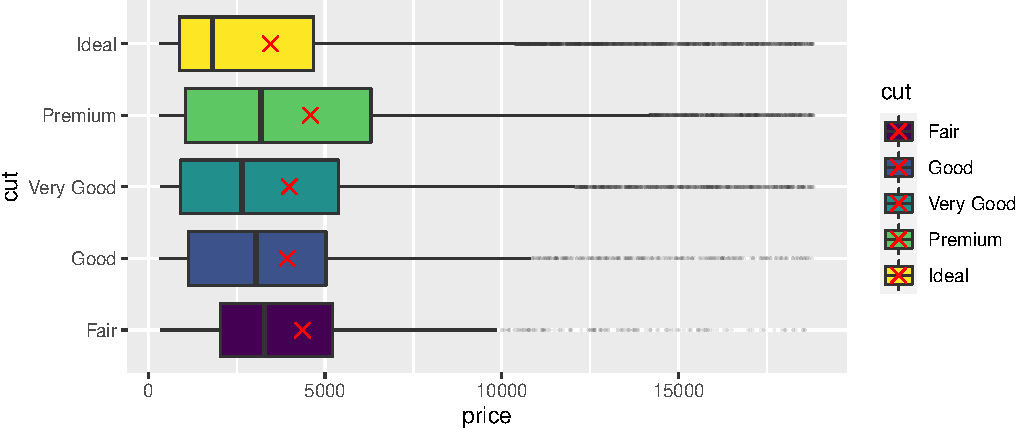
\includegraphics{_main_files/figure-latex/unnamed-chunk-4-1.pdf}

What do we notice about the relationship between price and cut? Is this
surprising?

\subsection{Histogram of carat size and quality of
cut}\label{histogram-of-carat-size-and-quality-of-cut}

Next, we examine a histogram, displaying price, cut, and carat size.

\begin{Shaded}
\begin{Highlighting}[]
\KeywordTok{ggplot}\NormalTok{(}\DataTypeTok{data=}\NormalTok{diamonds, }\KeywordTok{aes}\NormalTok{(}\DataTypeTok{x=}\NormalTok{carat, }\DataTypeTok{fill=}\NormalTok{cut)) }\OperatorTok{+}\StringTok{ }\KeywordTok{geom_histogram}\NormalTok{()}
\end{Highlighting}
\end{Shaded}

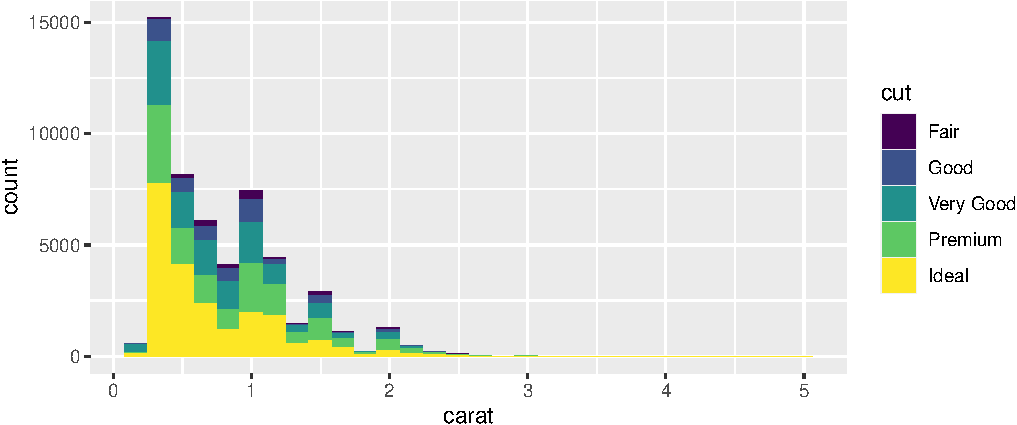
\includegraphics{_main_files/figure-latex/unnamed-chunk-5-1.pdf}

How does the information in this plot help explain the surprising result
we saw in the boxplot?

\subsection{Table 1: Average carat size and price by quality of
cut}\label{table-1-average-carat-size-and-price-by-quality-of-cut}

\begin{Shaded}
\begin{Highlighting}[]
\NormalTok{diamonds }\OperatorTok\StringTok{ }\KeywordTok{group_by}\NormalTok{(cut) }\OperatorTok\StringTok{ }\KeywordTok{summarize}\NormalTok{(}\DataTypeTok{N=}\KeywordTok{n}\NormalTok{(), }
                                         \DataTypeTok{Avg_carat=}\KeywordTok{mean}\NormalTok{(carat), }
                                         \DataTypeTok{Avg_price=}\KeywordTok{mean}\NormalTok{(price) )}
\end{Highlighting}
\end{Shaded}

\begin{verbatim}
## # A tibble: 5 x 4
##   cut           N Avg_carat Avg_price
##   <ord>     <int>     <dbl>     <dbl>
## 1 Fair       1610     1.05      4359.
## 2 Good       4906     0.849     3929.
## 3 Very Good 12082     0.806     3982.
## 4 Premium   13791     0.892     4584.
## 5 Ideal     21551     0.703     3458.
\end{verbatim}

\subsection{Scatterplot of carat size and quality of
cut}\label{scatterplot-of-carat-size-and-quality-of-cut}

Next, we use a scatterplot to visualize cut, price, and carat size.

\begin{Shaded}
\begin{Highlighting}[]
\KeywordTok{ggplot}\NormalTok{(}\DataTypeTok{data=}\NormalTok{diamonds, }\KeywordTok{aes}\NormalTok{(}\DataTypeTok{x=}\NormalTok{carat, }\DataTypeTok{y=}\NormalTok{price, }\DataTypeTok{color=}\NormalTok{cut)) }\OperatorTok{+}\StringTok{ }\KeywordTok{geom_point}\NormalTok{()}
\end{Highlighting}
\end{Shaded}

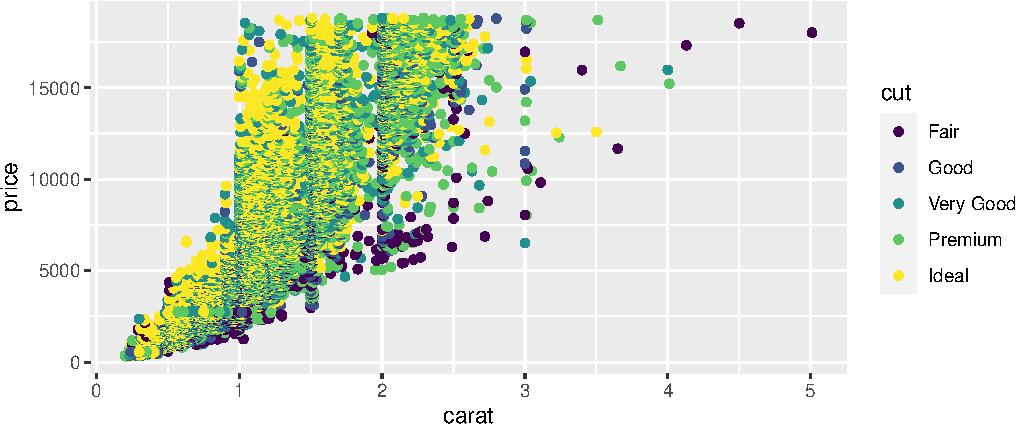
\includegraphics{_main_files/figure-latex/unnamed-chunk-7-1.pdf}

What should we conclude about the relationship between price and quality
of cut? Are better cuts generally more expensive? less expensive? about
the same? Does the relationship between price and cut seem to depend on
carat size?

\subsection{Terminology}\label{terminology}

The diamonds dataset is an example of two statistical concepts:

\textbf{Simpson's Paradox} refers to a situation when an apparent
relationship between two variables changes or reverses when additional
variable(s) are considered.\\
Example: diamonds with higher quality of cut appear less expensive than
lower quality cuts, until we account for carat size

An \textbf{interaction} between two variables X and Y occurs when the
relationship between X and a third variable Z depends on Y.\\
Example: the relationship between cut and price depends on carat size,
so there is an interaction between cut and carat size.

\section{Tidy Data}\label{tidy-data}

\subsection{Representations of Data}\label{representations-of-data}

Data can be displayed in many different tabular forms. We'll discuss one
useful form, called \textbf{tidy} data.

Learning Outcomes:

\begin{enumerate}
\def\labelenumi{\arabic{enumi}.}
\item
  Define tidy data.
\item
  Recognize when data are tidy form.
\end{enumerate}

Consider the following representations of the same dataset, which
dispays the number of tuberculosis cases in different countries,
relative to population. This example comes from
\href{https://r4ds.had.co.nz/tidy-data.html}{R for Data Science by
Wickham and Grolemund}

\subsection{Representation 1}\label{representation-1}

\begin{tabular}{l|r|r|r}
\hline
country & year & cases & population\\
\hline
Afghanistan & 1999 & 745 & 19987071\\
\hline
Afghanistan & 2000 & 2666 & 20595360\\
\hline
Brazil & 1999 & 37737 & 172006362\\
\hline
Brazil & 2000 & 80488 & 174504898\\
\hline
China & 1999 & 212258 & 1272915272\\
\hline
China & 2000 & 213766 & 1280428583\\
\hline
\end{tabular}

\subsection{Representation 2}\label{representation-2}

\begin{tabular}{l|r|l|r}
\hline
country & year & type & count\\
\hline
Afghanistan & 1999 & cases & 745\\
\hline
Afghanistan & 1999 & population & 19987071\\
\hline
Afghanistan & 2000 & cases & 2666\\
\hline
Afghanistan & 2000 & population & 20595360\\
\hline
Brazil & 1999 & cases & 37737\\
\hline
Brazil & 1999 & population & 172006362\\
\hline
Brazil & 2000 & cases & 80488\\
\hline
Brazil & 2000 & population & 174504898\\
\hline
China & 1999 & cases & 212258\\
\hline
China & 1999 & population & 1272915272\\
\hline
China & 2000 & cases & 213766\\
\hline
China & 2000 & population & 1280428583\\
\hline
\end{tabular}

\subsection{Representation 3}\label{representation-3}

\begin{tabular}{l|r|l}
\hline
country & year & rate\\
\hline
Afghanistan & 1999 & 745/19987071\\
\hline
Afghanistan & 2000 & 2666/20595360\\
\hline
Brazil & 1999 & 37737/172006362\\
\hline
Brazil & 2000 & 80488/174504898\\
\hline
China & 1999 & 212258/1272915272\\
\hline
China & 2000 & 213766/1280428583\\
\hline
\end{tabular}

\subsection{Representation 4}\label{representation-4}

Table A:

\begin{tabular}{l|r|r}
\hline
country & 1999 & 2000\\
\hline
Afghanistan & 745 & 2666\\
\hline
Brazil & 37737 & 80488\\
\hline
China & 212258 & 213766\\
\hline
\end{tabular}

Table B:

\begin{Shaded}
\begin{Highlighting}[]
\KeywordTok{kable}\NormalTok{(table4b)}
\end{Highlighting}
\end{Shaded}

\begin{tabular}{l|r|r}
\hline
country & 1999 & 2000\\
\hline
Afghanistan & 19987071 & 20595360\\
\hline
Brazil & 172006362 & 174504898\\
\hline
China & 1272915272 & 1280428583\\
\hline
\end{tabular}

\subsection{Variables and
Observations}\label{variables-and-observations}

In this example, we have observed data on various countries at different
points in time. The record for a single country, in a given year is
called an \textbf{observation}.

For each observation, we record the country, year, number of cases, and
population. These are called \textbf{variables.}

\subsection{Tidy Data}\label{tidy-data-1}

A dataset is said to be \textbf{tidy} when it satisfies the following
conditions:

\begin{enumerate}
\def\labelenumi{\arabic{enumi}.}
\tightlist
\item
  Each variable has its own column.\\
\item
  Each observation has its own row.\\
\item
  Each value must has own cell.
\end{enumerate}

In fact, any two of these imply the third.

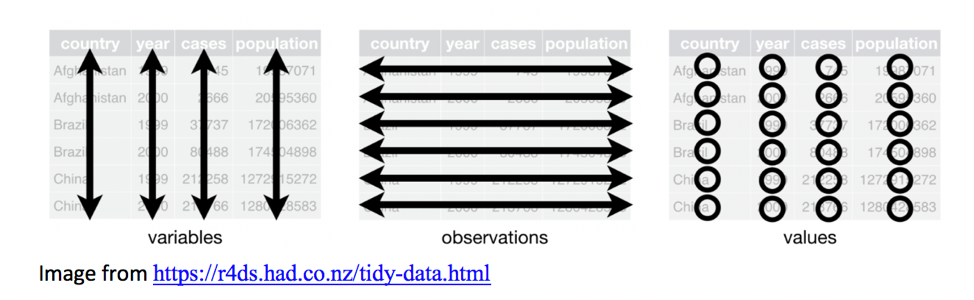
\includegraphics[width=0.9\linewidth]{Tidy_Data}

Image from \href{https://r4ds.had.co.nz/tidy-data.html}{R for Data
Science by Wickham and Grolemund}

\subsection{Representation 1 Tidy}\label{representation-1-tidy}

Representation 1 is in tidy form.

\begin{tabular}{l|r|r|r}
\hline
country & year & cases & population\\
\hline
Afghanistan & 1999 & 745 & 19987071\\
\hline
Afghanistan & 2000 & 2666 & 20595360\\
\hline
Brazil & 1999 & 37737 & 172006362\\
\hline
Brazil & 2000 & 80488 & 174504898\\
\hline
China & 1999 & 212258 & 1272915272\\
\hline
China & 2000 & 213766 & 1280428583\\
\hline
\end{tabular}

\subsection{Representation 2 not Tidy}\label{representation-2-not-tidy}

Representation 2 is not in tidy form.

\begin{itemize}
\tightlist
\item
  Observations are spread over multiple rows.\\
\item
  The variables \texttt{cases} and \texttt{population} do not have thir
  own column.\\
\item
  The column \texttt{type} contains variable names, not values.
\end{itemize}

\begin{tabular}{l|r|l|r}
\hline
country & year & type & count\\
\hline
Afghanistan & 1999 & cases & 745\\
\hline
Afghanistan & 1999 & population & 19987071\\
\hline
Afghanistan & 2000 & cases & 2666\\
\hline
Afghanistan & 2000 & population & 20595360\\
\hline
Brazil & 1999 & cases & 37737\\
\hline
Brazil & 1999 & population & 172006362\\
\hline
Brazil & 2000 & cases & 80488\\
\hline
Brazil & 2000 & population & 174504898\\
\hline
China & 1999 & cases & 212258\\
\hline
China & 1999 & population & 1272915272\\
\hline
China & 2000 & cases & 213766\\
\hline
China & 2000 & population & 1280428583\\
\hline
\end{tabular}

\subsection{Representation 3 not Tidy}\label{representation-3-not-tidy}

Representation 3 is not in tidy form.

The variables \texttt{cases} and \texttt{population} do not have their
own columns, but are combined in a single column called \texttt{rate}.

\begin{tabular}{l|r|l}
\hline
country & year & rate\\
\hline
Afghanistan & 1999 & 745/19987071\\
\hline
Afghanistan & 2000 & 2666/20595360\\
\hline
Brazil & 1999 & 37737/172006362\\
\hline
Brazil & 2000 & 80488/174504898\\
\hline
China & 1999 & 212258/1272915272\\
\hline
China & 2000 & 213766/1280428583\\
\hline
\end{tabular}

\subsection{Representation 4 is not
Tidy}\label{representation-4-is-not-tidy}

Representation 4 is not in tidy form.

\begin{itemize}
\tightlist
\item
  The variable \texttt{year} is spread across multiple columns.\\
\item
  The variables \texttt{cases} and \texttt{population} are spread over
  multiple tables.
\end{itemize}

\begin{tabular}{l|r|r}
\hline
country & 1999 & 2000\\
\hline
Afghanistan & 745 & 2666\\
\hline
Brazil & 37737 & 80488\\
\hline
China & 212258 & 213766\\
\hline
\end{tabular}

\begin{tabular}{l|r|r}
\hline
country & 1999 & 2000\\
\hline
Afghanistan & 19987071 & 20595360\\
\hline
Brazil & 172006362 & 174504898\\
\hline
China & 1272915272 & 1280428583\\
\hline
\end{tabular}

\subsection{Why Use Tidy Data}\label{why-use-tidy-data}

\begin{itemize}
\item
  Data are often easiest to work with when they are in tidy form
\item
  The \texttt{tidyverse()} R package is useful for creating graphs, and
  calculating summary statistics when data are in tidy form.
\item
  Sometimes there is good reason for data to not be in tidy form. This
  is ok, but it makes it harder to work with.
\item
  In this class, we will focus on data that are already in tidy form.
  However, if you come across data on your own, you should check that it
  is tidy before attempting to use the techniques we'll see in this
  class.
\item
  In \textbf{CMSC/STAT 205: Data-Scientific Programming,} we study how
  to convert data into tidy form if it is not already. More information
  can be found in \href{https://r4ds.had.co.nz/tidy-data.html}{R For
  Data Science by Wickham and Grolemund}.
\end{itemize}

\chapter{Introduction to Linear
Models}\label{introduction-to-linear-models}

\section{Models with a Categorical Explanatory
Variable}\label{models-with-a-categorical-explanatory-variable}

\subsection{Models with a Categorical Explanatory
Variable}\label{models-with-a-categorical-explanatory-variable-1}

Learning outcomes:

\begin{enumerate}
\def\labelenumi{\arabic{enumi}.}
\tightlist
\item
  Fit model with categorical variables using R.\\
\item
  Interpret model coefficients.\\
\item
  Make predictions.\\
\item
  Calculate proportion of variation explained by model.
\end{enumerate}

We'll work with a set of 10 houses sold in Ames, IA between 2006 and
2010.

\subsection{Variation in Ames IA, House
Prices}\label{variation-in-ames-ia-house-prices}

Shown below are the prices of 10 houses sold in Ames, IA between 2006
and 2010.

\begin{verbatim}
##  [1] 123.00 187.00 176.50 113.00 163.99 110.00  84.90 150.00 235.00 137.00
\end{verbatim}

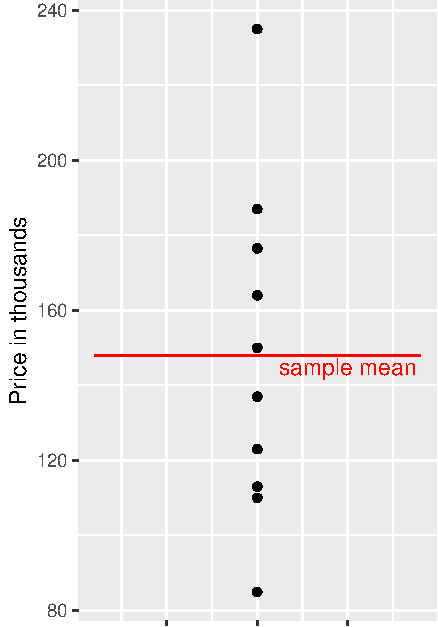
\includegraphics{_main_files/figure-latex/unnamed-chunk-21-1.pdf}

\subsection{Predicting Price of New
House}\label{predicting-price-of-new-house}

Shown below are the prices of 10 houses sold in Ames, IA between 2006
and 2010.

\begin{verbatim}
##  [1] 123.00 187.00 176.50 113.00 163.99 110.00  84.90 150.00 235.00 137.00
\end{verbatim}

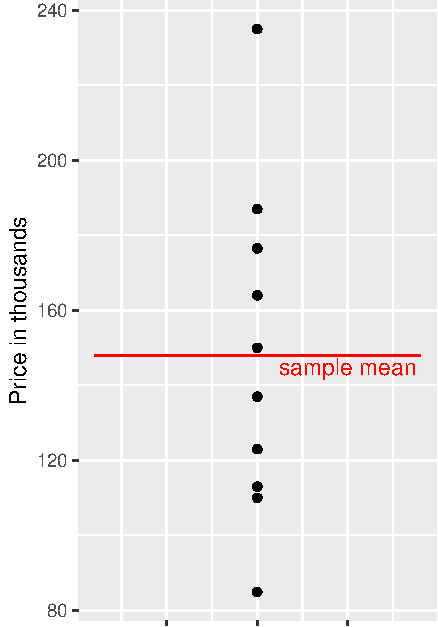
\includegraphics{_main_files/figure-latex/unnamed-chunk-24-1.pdf}

\begin{itemize}
\item
  Suppose we want to predict the price of a new house, that was sold in
  this time period. (note that new means a house not among the original
  10, rather than a newly-built house.)
\item
  Using the information available the best we can do is to use the
  sample mean for our prediction.
\end{itemize}

\begin{Shaded}
\begin{Highlighting}[]
\KeywordTok{mean}\NormalTok{(Houses}\OperatorTok{$}\NormalTok{SalePrice)}
\end{Highlighting}
\end{Shaded}

\begin{verbatim}
## [1] 148.039
\end{verbatim}

\subsection{A Very Simple Model}\label{a-very-simple-model}

\begin{itemize}
\tightlist
\item
  If we have the prices of \(n\) houses, \(y_i, y_2, \ldots, y_n\), and
  want to predict the price of a new house, we use the model:
\end{itemize}

\[
\widehat{\text{Price}} = \bar{y},  \text{where } \bar{y}=\frac{\displaystyle\sum_{i=1}^ny_i}{n}\].

\begin{itemize}
\tightlist
\item
  The symbol \(\widehat{\text{Price}}\), represents the predicted, or
  expected, price.
\end{itemize}

\subsection{Simple Model in R}\label{simple-model-in-r}

\begin{Shaded}
\begin{Highlighting}[]
\NormalTok{M0 <-}\StringTok{ }\KeywordTok{lm}\NormalTok{(}\DataTypeTok{data=}\NormalTok{Houses, SalePrice}\OperatorTok{~}\DecValTok{1}\NormalTok{)}
\KeywordTok{summary}\NormalTok{(M0)}
\end{Highlighting}
\end{Shaded}

\begin{verbatim}
## 
## Call:
## lm(formula = SalePrice ~ 1, data = Houses)
## 
## Residuals:
##     Min      1Q  Median      3Q     Max 
## -63.139 -32.539  -4.539  25.334  86.961 
## 
## Coefficients:
##             Estimate Std. Error t value  Pr(>|t|)    
## (Intercept)   148.04      13.97    10.6 0.0000022 ***
## ---
## Signif. codes:  0 '***' 0.001 '**' 0.01 '*' 0.05 '.' 0.1 ' ' 1
## 
## Residual standard error: 44.17 on 9 degrees of freedom
\end{verbatim}

\subsection{Quantifying Total Variability in
Prices}\label{quantifying-total-variability-in-prices}

\begin{itemize}
\item
  Although the mean price represents our best prediction, we certainly
  shouldn't expect the price of the new house to exactly match the mean
  of the original 10. There is considerable variability between house
  prices.
\item
  We can get a sense of how much variability we should expect in our
  prediction by looking at how much the values in our dataset differ
  from the predicted (mean) price.
\item
  \(\displaystyle\sum_{i=1}^n (y_i - \bar{y})=0\), so this is not a
  helpful measure.
\end{itemize}

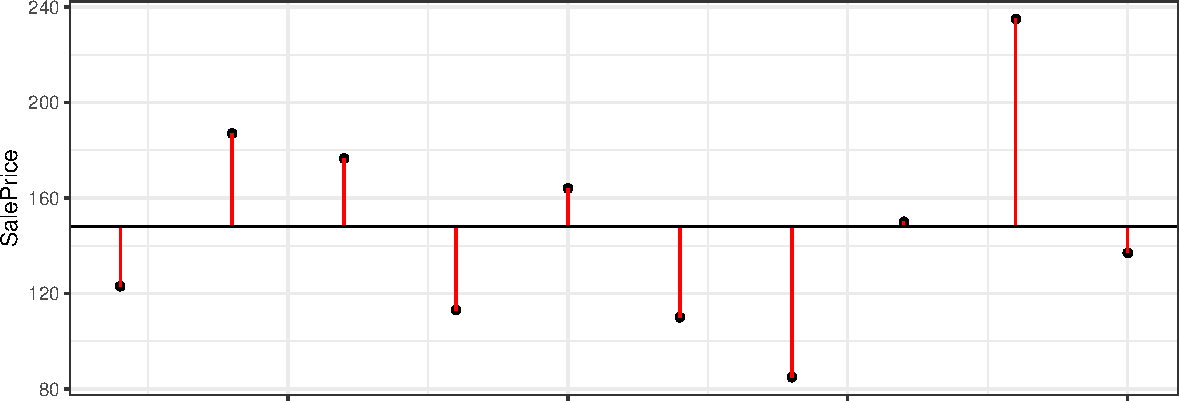
\includegraphics{_main_files/figure-latex/unnamed-chunk-27-1.pdf}

\subsection{Total Sum of Squares}\label{total-sum-of-squares}

We'll measure total variability in price, using :

\[
\displaystyle\sum_{i=1}^n (y_i - \bar{y})^2
\]

We'll call this the total sum of squares, and abbreviate it SST.

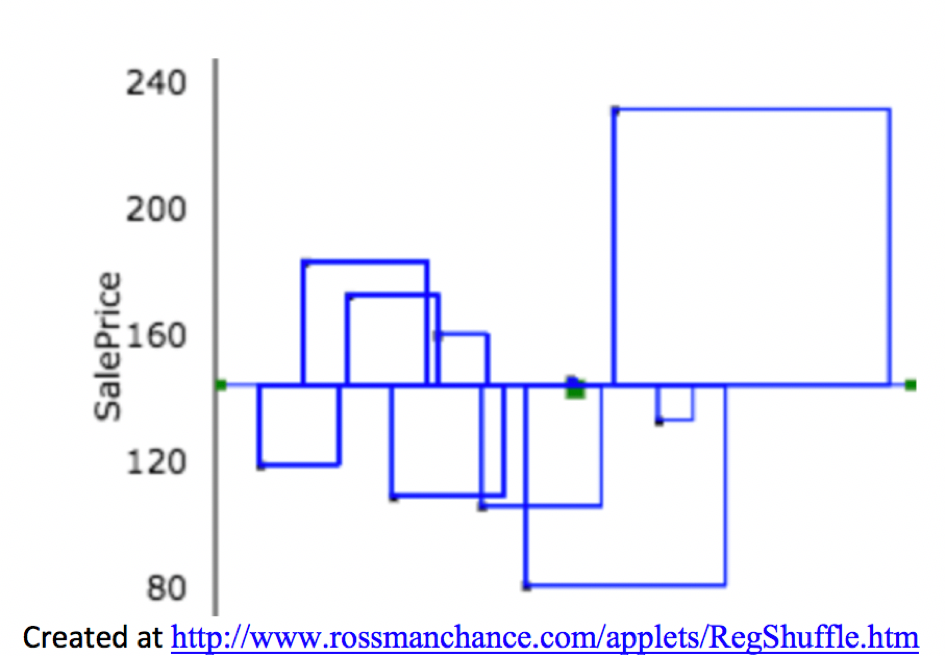
\includegraphics[width=13.12in,height=0.65\textheight]{SST}

\subsection{Total Variation Calculations in Simple
Model}\label{total-variation-calculations-in-simple-model}

\begin{itemize}
\tightlist
\item
  Calculate \(\displaystyle\sum_{i=1}^n (y_i - \bar{y})\) in R.
\end{itemize}

\begin{Shaded}
\begin{Highlighting}[]
\KeywordTok{sum}\NormalTok{(Houses}\OperatorTok{$}\NormalTok{SalePrice }\OperatorTok{-}\StringTok{ }\KeywordTok{mean}\NormalTok{(Houses}\OperatorTok{$}\NormalTok{SalePrice))}
\end{Highlighting}
\end{Shaded}

\begin{verbatim}
## [1] 0.0000000000001421085
\end{verbatim}

\begin{itemize}
\tightlist
\item
  Calculate \(SST = \displaystyle\sum_{i=1}^n (y_i - \bar{y})^2\) in R.
\end{itemize}

\begin{Shaded}
\begin{Highlighting}[]
\KeywordTok{sum}\NormalTok{((Houses}\OperatorTok{$}\NormalTok{SalePrice }\OperatorTok{-}\StringTok{ }\KeywordTok{mean}\NormalTok{(Houses}\OperatorTok{$}\NormalTok{SalePrice))}\OperatorTok{^}\DecValTok{2}\NormalTok{)}
\end{Highlighting}
\end{Shaded}

\begin{verbatim}
## [1] 17558.52
\end{verbatim}

\subsection{Adding Information about
Neighborhood}\label{adding-information-about-neighborhood}

\begin{itemize}
\item
  Now, suppose we know the neighborhood of each house. We can use this
  information to improve our predictions.
\item
  The prediction for a new house is given by the average price in that
  neighborhood.
\end{itemize}

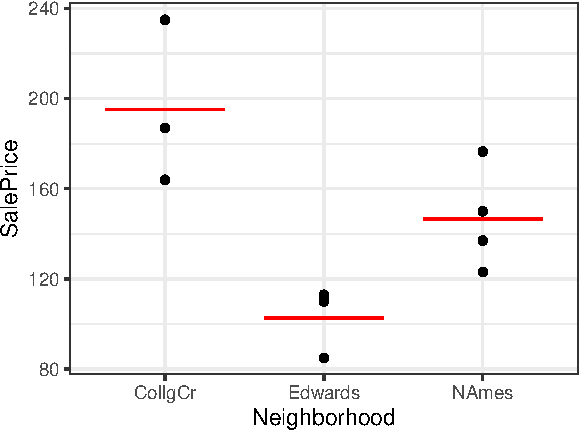
\includegraphics{_main_files/figure-latex/unnamed-chunk-32-1.pdf}

\begin{tabular}{l|r}
\hline
Neighborhood & AveragePrice\\
\hline
CollgCr & 195.3300\\
\hline
Edwards & 102.6333\\
\hline
NAmes & 146.6250\\
\hline
\end{tabular}

\subsection{Explanatory and Response
Variables}\label{explanatory-and-response-variables}

\begin{itemize}
\item
  The variable we are trying to predict (price) is called the
  \textbf{response variable} (denoted \(Y\)).
\item
  The variable(s) we use to help us make the prediction (neighborhood)
  is(are) called \textbf{explanatory variables} (denoted \(X\)). These
  are also referred to as \textbf{predictor variables} or
  \textbf{covariates}.
\end{itemize}

\subsection{Model by Neighborhood}\label{model-by-neighborhood}

\begin{Shaded}
\begin{Highlighting}[]
\NormalTok{M_Nbhd <-}\StringTok{ }\KeywordTok{lm}\NormalTok{(}\DataTypeTok{data=}\NormalTok{Houses, SalePrice }\OperatorTok{~}\StringTok{ }\NormalTok{Neighborhood)}
\KeywordTok{summary}\NormalTok{(M_Nbhd)}
\end{Highlighting}
\end{Shaded}

\begin{verbatim}
## 
## Call:
## lm(formula = SalePrice ~ Neighborhood, data = Houses)
## 
## Residuals:
##     Min      1Q  Median      3Q     Max 
## -31.340 -15.706  -2.477   9.617  39.670 
## 
## Coefficients:
##                     Estimate Std. Error t value   Pr(>|t|)    
## (Intercept)           195.33      14.89  13.118 0.00000349 ***
## NeighborhoodEdwards   -92.70      21.06  -4.402    0.00315 ** 
## NeighborhoodNAmes     -48.71      19.70  -2.473    0.04267 *  
## ---
## Signif. codes:  0 '***' 0.001 '**' 0.01 '*' 0.05 '.' 0.1 ' ' 1
## 
## Residual standard error: 25.79 on 7 degrees of freedom
## Multiple R-squared:  0.7348, Adjusted R-squared:  0.6591 
## F-statistic: 9.699 on 2 and 7 DF,  p-value: 0.009603
\end{verbatim}

\subsection{R Output for Model with Categorical
Variables}\label{r-output-for-model-with-categorical-variables}

\begin{verbatim}
##                      Estimate Std. Error   t value       Pr(>|t|)
## (Intercept)         195.33000   14.89037 13.117871 0.000003490079
## NeighborhoodEdwards -92.69667   21.05817 -4.401934 0.003149456985
## NeighborhoodNAmes   -48.70500   19.69811 -2.472572 0.042671888138
\end{verbatim}

\begin{itemize}
\tightlist
\item
  For categorical explanatory variables, R treats the category that
  comes first alphabetically (in this case CCreek), as a baseline. The
  intercept gives the prediction for this category.

  \begin{itemize}
  \tightlist
  \item
    We would expect a house in College Creek to cost 195.33 thousand
    dollars.
  \end{itemize}
\item
  Each of the other rows in the coefficients table represent the
  difference between the expected response (price) for that category
  (neighborhood), compared to the baseline.

  \begin{itemize}
  \tightlist
  \item
    We would expect a house in Edwards to cost 92.70 thousand less than
    a house in College Creek. (hence costing 102.63 thousand)\\
  \item
    We would expect a house in North Ames to cost 48.71 thousand less
    than a house in College Creek. (hence costing 146.62 thousand)
  \end{itemize}
\end{itemize}

\subsection{Model Notation for Houses by
Neighborhood}\label{model-notation-for-houses-by-neighborhood}

In the model can be expressed in the form:

\(\widehat{\text{Price}}= b_0+ b_1 \times\text{I}_{\text{Edwards}} +b_2 \times\text{I}_{\text{NAmes}}\)

\(\widehat{\text{Price}}= 195.33+ -92.7 \times\text{I}_{\text{Edwards}} +-48.71 \times\text{I}_{\text{NAmes}}\),
where

\text{I} represents an indicator variables, taking on values 0 or 1.\\
- Example: \[ \text{I}_{\text{Edwards}} =\begin{cases} 
      1 & \text{if house is in Edwards Neighborhood} \\
      0 & \text{otherwise}
       \end{cases}
      \]

\textbf{Predicted Prices:}

College Creek:
\(\widehat{\text{Price}}= 195.33+ -92.7 \times0 +-48.71 \times0 = 195.33\)
thousand.

Edwards:
\(\widehat{\text{Price}}= 195.33+ -92.7 \times1 +-48.71 \times0 = 102.63\)
thousand.

North Ames:
\(\widehat{\text{Price}}= 195.33+ -92.7 \times0 +-48.71 \times1 = 146.62\)
thousand.

\subsection{Residuals for Neighborhood
Model}\label{residuals-for-neighborhood-model}

\begin{itemize}
\tightlist
\item
  The difference between the true and predicted values
  (\(y_i - \hat{y}_i\)) is called the \(ith\) \textbf{residual}.
\end{itemize}

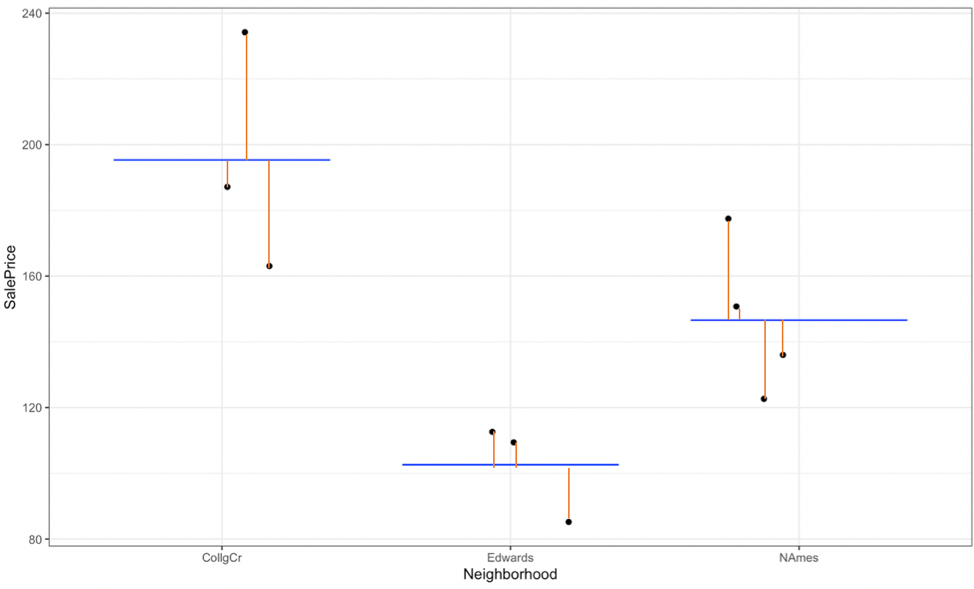
\includegraphics[width=0.75\linewidth]{Cat_Resid}

\subsection{Residuals for Neighborhood Model
(cont.)}\label{residuals-for-neighborhood-model-cont.}

\begin{verbatim}
##    SalePrice Predicted   Residual ResidualSq
## 1     123.00  146.6250 -23.625000  558.14063
## 2     187.00  195.3300  -8.330000   69.38890
## 3     176.50  146.6250  29.875000  892.51563
## 4     113.00  102.6333  10.366667  107.46778
## 5     163.99  195.3300 -31.340000  982.19560
## 6     110.00  102.6333   7.366667   54.26778
## 7      84.90  102.6333 -17.733333  314.47111
## 8     150.00  146.6250   3.375000   11.39063
## 9     235.00  195.3300  39.670000 1573.70890
## 10    137.00  146.6250  -9.625000   92.64062
\end{verbatim}

\begin{Shaded}
\begin{Highlighting}[]
\KeywordTok{sum}\NormalTok{(M_Nbhd}\OperatorTok{$}\NormalTok{residuals}\OperatorTok{^}\DecValTok{2}\NormalTok{)}
\end{Highlighting}
\end{Shaded}

\begin{verbatim}
## [1] 4656.188
\end{verbatim}

\subsection{Variability Explained by Model with
Neighborhood}\label{variability-explained-by-model-with-neighborhood}

Intercept-Only Model:

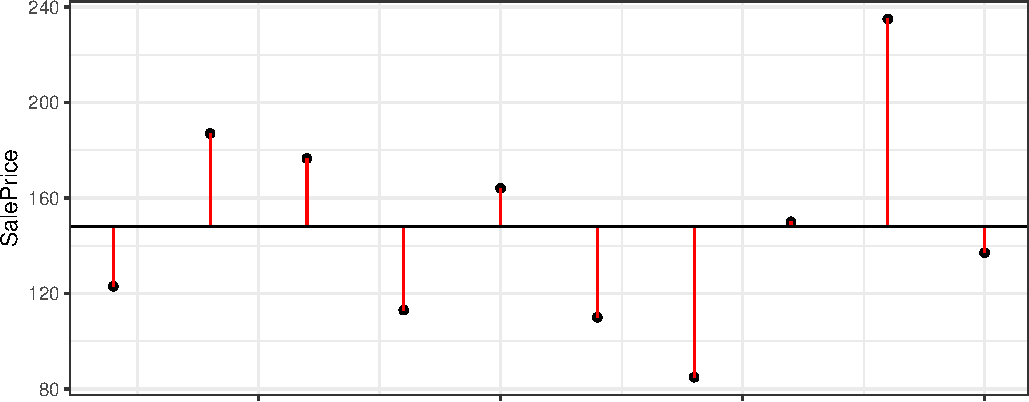
\includegraphics{_main_files/figure-latex/unnamed-chunk-41-1.pdf}

\begin{Shaded}
\begin{Highlighting}[]
\KeywordTok{sum}\NormalTok{(M0}\OperatorTok{$}\NormalTok{residuals}\OperatorTok{^}\DecValTok{2}\NormalTok{)}
\end{Highlighting}
\end{Shaded}

\begin{verbatim}
## [1] 17558.52
\end{verbatim}

Model Using Neighborhood

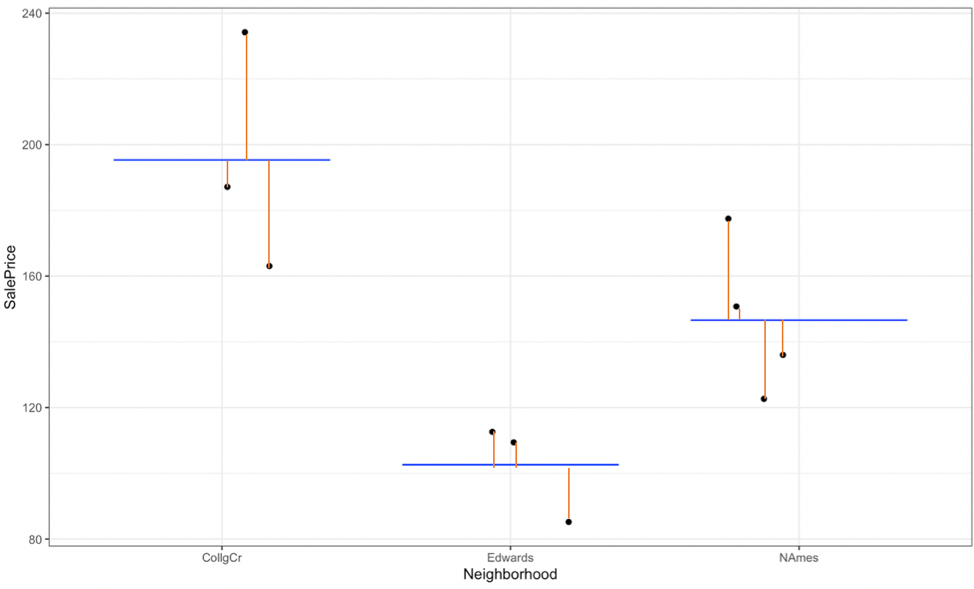
\includegraphics[width=13.53in]{Cat_Resid}

\begin{Shaded}
\begin{Highlighting}[]
\KeywordTok{sum}\NormalTok{(M_Nbhd}\OperatorTok{$}\NormalTok{residuals}\OperatorTok{^}\DecValTok{2}\NormalTok{)}
\end{Highlighting}
\end{Shaded}

\begin{verbatim}
## [1] 4656.188
\end{verbatim}

\subsection{Quantifying Variability
Explained}\label{quantifying-variability-explained}

\begin{itemize}
\tightlist
\item
  the total variability in house prices is the sum of the squared
  differences between price and average price.
\end{itemize}

\[\text{Total Variability in Price}= \text{SST} =\displaystyle\sum_{i=1}^n(y_i-\bar{y})^2\]

\begin{itemize}
\tightlist
\item
  the variability remaining unexplained even after accounting for
  neighborhood is given by the sum of squared residuals. We abbreviate
  this SSR, for sum of squared residuals.
\end{itemize}

\[
\text{SSR} = \text{Variability Remaining}=\displaystyle\sum_{i=1}^n(y_i-\hat{y}_i)^2
\]

\begin{itemize}
\tightlist
\item
  the variability explained by the model, abbreviated SSM, is given by
\end{itemize}

\[ \text{SSM} = \text{SST} - \text{SSR} \]

It can be shown that
\(\text{SSM}=\displaystyle\sum_{i=1}^n(\hat{y}_i-\bar{y})^2\). These
abbreviations here vary across texts. Be careful!

\subsection{Coefficient of
Determination}\label{coefficient-of-determination}

\begin{itemize}
\tightlist
\item
  The \textbf{coefficient of determination (abbreviated \(R^2\))} is
  defined as
\end{itemize}

\[R^2=\frac{\text{Variability Explained by Model}}{\text{Total Variability}}=\frac{\text{SSM}}{\text{SST}} =\frac{\displaystyle\sum_{i=1}^n(\hat{y}_i-\bar{y})^2}{\displaystyle\sum_{i=1}^n(y_i-\bar{y})^2}\]

\begin{itemize}
\tightlist
\item
  \(R^2\) can be interpreted as the proportion of total variability in
  the response variable that is explained by the model using the given
  explanatory variable(s).
\end{itemize}

\subsection{\texorpdfstring{\(R^2\)
Visually}{R\^{}2 Visually}}\label{r2-visually}

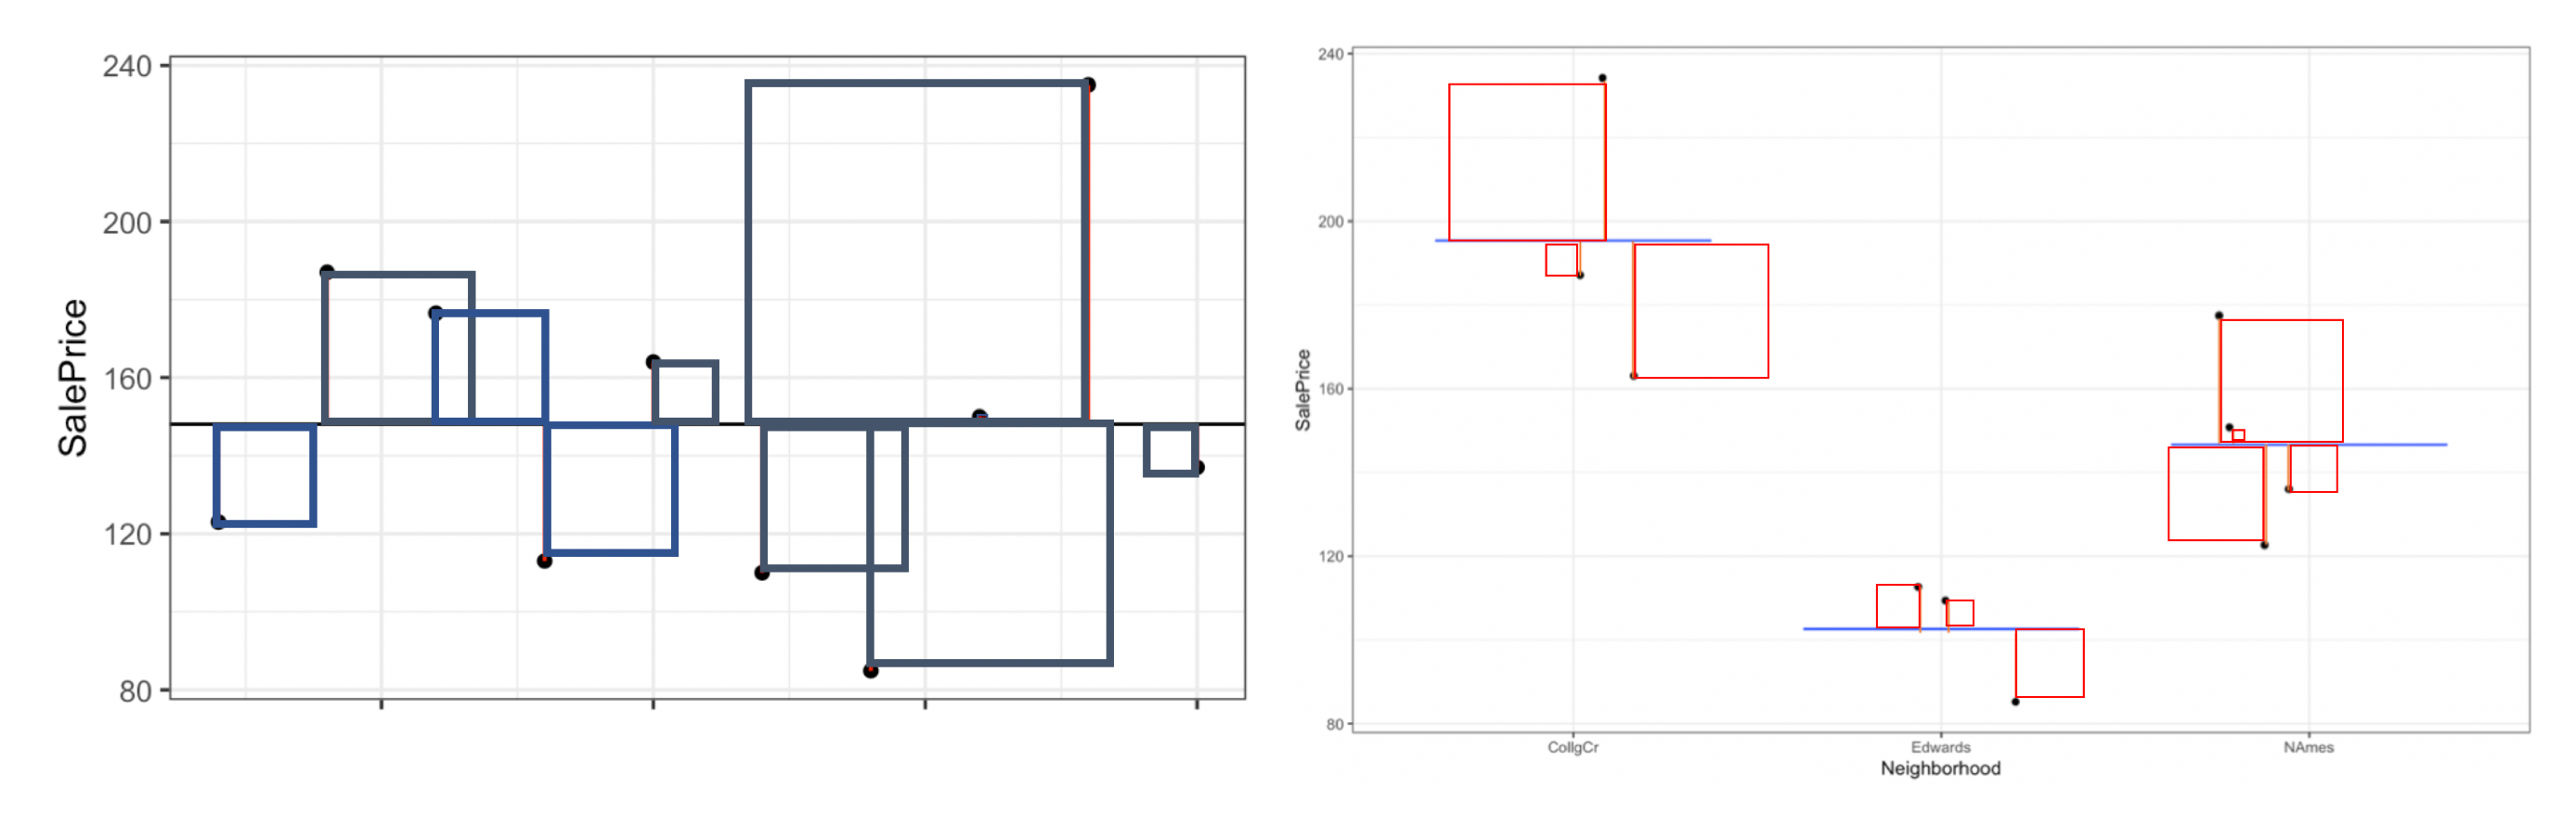
\includegraphics[width=1\linewidth]{Rsq2}

\begin{itemize}
\item
  Blue Area = Total Variability (SST)
\item
  Red Area = Variability Remaining Unexplained by Model (SSR)
\item
  Blue Area - Red Area = Variability Explained by Model (SSM)
\item
  \(R^2 = \frac{\text{Area of Blue Squares} - \text{Area of Red Squares}}{\text{Area of Blue Squares}} = \frac{\text{SST}-\text{SSR}}{\text{SST}}= \frac{\text{SSM}}{\text{SST}}\)
\end{itemize}

\subsection{Variation Explained by Neighborhood
Model}\label{variation-explained-by-neighborhood-model}

\begin{itemize}
\tightlist
\item
  Total variability in house prices SST = 17,558.52\\
\item
  Variability remaining unexplained after model accounting for
  neighborhood: SSR =4,656.188\\
\item
  Variability explained by model: SSM=SST-SSR=17,558.52 - 4,656.188 =
  12,901.81
\end{itemize}

\[ R^2= \frac{12,901.81}{17,558.52}\approx0.7348 \]

\begin{itemize}
\item
  73.5\% of the variation in house price is explained by the model using
  neighborhood as an explanatory variable.
\item
  This matches the value of ``Multiple R-squared'' in the 2nd last line
  of the R model summary.
\end{itemize}

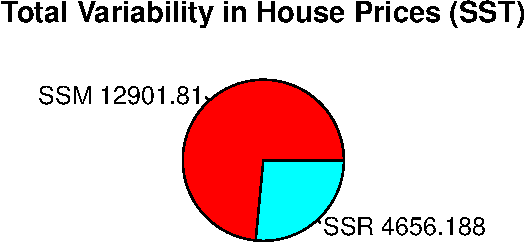
\includegraphics{_main_files/figure-latex/unnamed-chunk-46-1.pdf}

\section{Models with a Quantitative Explanatory
Variable}\label{models-with-a-quantitative-explanatory-variable}

\subsection{Model using SquareFeet in
House}\label{model-using-squarefeet-in-house}

Now, suppose we do not know the neighborhood, but do know the size of
the house in square feet.

\begin{Shaded}
\begin{Highlighting}[]
\KeywordTok{ggplot}\NormalTok{(}\DataTypeTok{data=}\NormalTok{Houses, }\KeywordTok{aes}\NormalTok{(}\DataTypeTok{x=}\NormalTok{SquareFeet, }\DataTypeTok{y=}\NormalTok{SalePrice)) }\OperatorTok{+}\StringTok{ }\KeywordTok{geom_point}\NormalTok{() }
\end{Highlighting}
\end{Shaded}

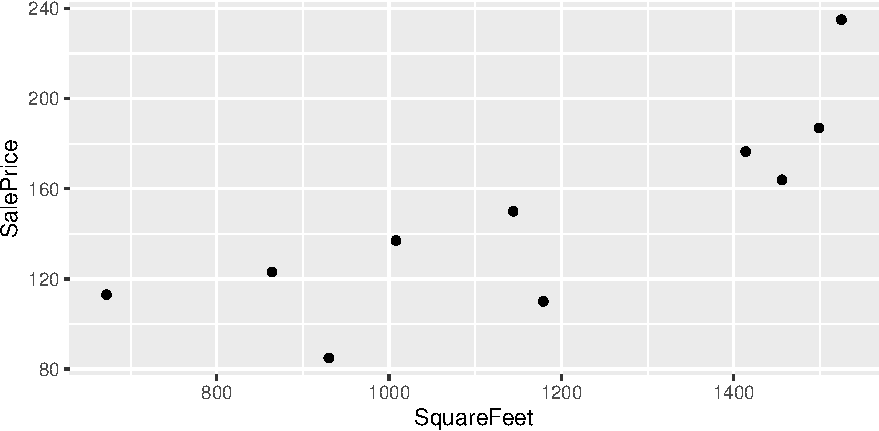
\includegraphics{_main_files/figure-latex/unnamed-chunk-47-1.pdf}

Suppose we want to predict the price of houses with the following number
of square feet:

\begin{itemize}
\tightlist
\item
  990 square feet\\
\item
  1235 square feet\\
\item
  1476 square feet
\end{itemize}

\subsection{Model on SquareFeet in
House}\label{model-on-squarefeet-in-house}

Since square feet is a quantitative variable, we can make predictions by
fitting a line to the data.

\begin{Shaded}
\begin{Highlighting}[]
\KeywordTok{ggplot}\NormalTok{(}\DataTypeTok{data=}\NormalTok{Houses, }\KeywordTok{aes}\NormalTok{(}\DataTypeTok{x=}\NormalTok{SquareFeet, }\DataTypeTok{y=}\NormalTok{SalePrice)) }\OperatorTok{+}\StringTok{ }\KeywordTok{geom_point}\NormalTok{() }\OperatorTok{+}\StringTok{ }
\StringTok{  }\KeywordTok{stat_smooth}\NormalTok{(}\DataTypeTok{method=}\StringTok{"lm"}\NormalTok{, }\DataTypeTok{se=}\OtherTok{FALSE}\NormalTok{)}
\end{Highlighting}
\end{Shaded}

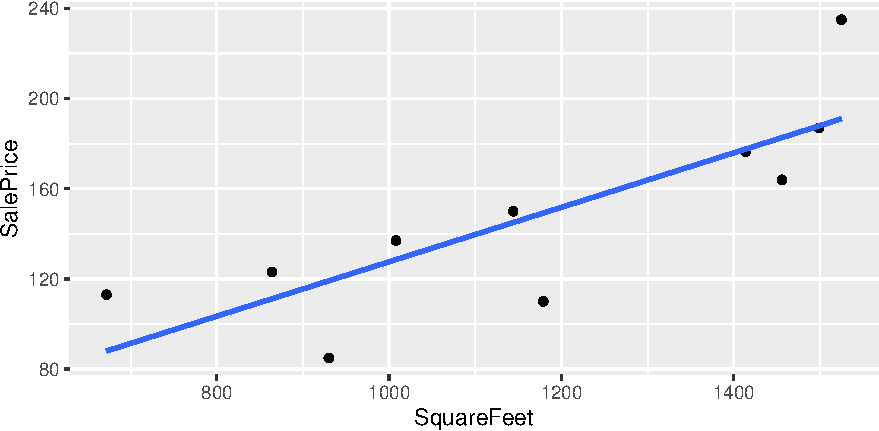
\includegraphics{_main_files/figure-latex/unnamed-chunk-48-1.pdf}

\begin{itemize}
\tightlist
\item
  For a house with 990 square feet, predicted price is about \$125
  thousand.\\
\item
  For a house with 1235 square feet, predicted price is about \$155
  thousand.\\
\item
  For a house with 1476 square feet, predicted price is about \$185
  thousand.
\end{itemize}

\subsection{Model using Square Feet}\label{model-using-square-feet}

\begin{Shaded}
\begin{Highlighting}[]
\NormalTok{M_SqFt <-}\StringTok{ }\KeywordTok{lm}\NormalTok{(}\DataTypeTok{data=}\NormalTok{Houses, SalePrice}\OperatorTok{~}\NormalTok{SquareFeet) }
\KeywordTok{summary}\NormalTok{(M_SqFt)}
\end{Highlighting}
\end{Shaded}

\begin{verbatim}
## 
## Call:
## lm(formula = SalePrice ~ SquareFeet, data = Houses)
## 
## Residuals:
##     Min      1Q  Median      3Q     Max 
## -39.235 -14.309   2.052  10.966  43.971 
## 
## Coefficients:
##             Estimate Std. Error t value Pr(>|t|)   
## (Intercept)  6.82000   36.35455   0.188  0.85586   
## SquareFeet   0.12079    0.03022   3.997  0.00397 **
## ---
## Signif. codes:  0 '***' 0.001 '**' 0.01 '*' 0.05 '.' 0.1 ' ' 1
## 
## Residual standard error: 27.06 on 8 degrees of freedom
## Multiple R-squared:  0.6663, Adjusted R-squared:  0.6246 
## F-statistic: 15.97 on 1 and 8 DF,  p-value: 0.003967
\end{verbatim}

\subsection{Model for SquareFeet and
Interpretations}\label{model-for-squarefeet-and-interpretations}

In the model using both square feet and neighborhood, the regression
equation is

\(\widehat{\text{Price}}= b_0+ b_1 \times\text{SquareFeet}\)

\(\widehat{\text{Price}}= 6.82+ 0.121 \times\text{SquareFeet}\)

\begin{itemize}
\item
  \(\widehat{\text{Price}}\) represents the expected, or predicted,
  price.
\item
  The slope, \(b_1\) represents the expected change in price (in
  thousands) per one-unit increase in square feet.

  \begin{itemize}
  \tightlist
  \item
    The price of a house is expected to increase by 121 dollars for each
    additional square foot.
  \end{itemize}
\item
  The intercept, \(b_0\) represents the expected price of a house with 0
  square feet.

  \begin{itemize}
  \tightlist
  \item
    In this situation, this is not a meaningful interpretation.
  \end{itemize}
\end{itemize}

\subsection{Calculating Predicted
Prices}\label{calculating-predicted-prices}

\(\widehat{\text{Price}}= 6.82+ 0.121 \times\text{SquareFeet}\)

\begin{itemize}
\tightlist
\item
  Predicted price for a house with 990 square feet:
\end{itemize}

\(\widehat{\text{Price}}= 6.82+ 0.121 \times990 = 126.4\) thousand
dollars.

\begin{itemize}
\tightlist
\item
  Predicted price for a house with 1235 square feet:
\end{itemize}

\(\widehat{\text{Price}}= 6.82+ 0.121 \times1235 = 156.0\) thousand
dollars.

\begin{itemize}
\tightlist
\item
  Predicted price for a house with with 1476 square feet:
\end{itemize}

\(\widehat{\text{Price}}= 6.82+ 0.121 \times1476 = 185.1\) thousand
dollars.

\subsection{Residuals for SquareFeet
Model}\label{residuals-for-squarefeet-model}

The difference between the actual and predicted price is called the
\textbf{residual.}

\begin{Shaded}
\begin{Highlighting}[]
\NormalTok{M_SqFt}\OperatorTok{$}\NormalTok{residuals}
\end{Highlighting}
\end{Shaded}

\begin{verbatim}
##           1           2           3           4           5           6 
##  11.8149181  -0.8885824  -1.1211847  25.0071576 -18.7044870 -39.2348498 
##           7           8           9          10 
## -34.2574142   4.9929021  43.9708019   8.4207385
\end{verbatim}

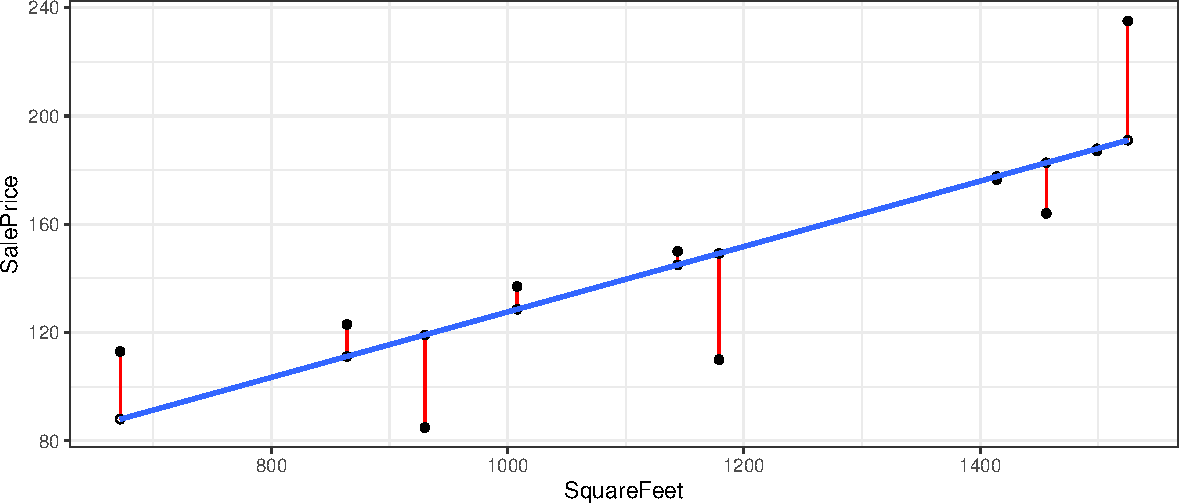
\includegraphics{_main_files/figure-latex/unnamed-chunk-52-1.pdf}

\subsection{Residuals for SquareFeet Model
(cont.)}\label{residuals-for-squarefeet-model-cont.}

\begin{verbatim}
##    SalePrice Predicted    Residual   ResidualSq
## 1     123.00 111.18508  11.8149181  139.5922893
## 2     187.00 187.88858  -0.8885824    0.7895786
## 3     176.50 177.62118  -1.1211847    1.2570550
## 4     113.00  87.99284  25.0071576  625.3579304
## 5     163.99 182.69449 -18.7044870  349.8578356
## 6     110.00 149.23485 -39.2348498 1539.3734427
## 7      84.90 119.15741 -34.2574142 1173.5704309
## 8     150.00 145.00710   4.9929021   24.9290718
## 9     235.00 191.02920  43.9708019 1933.4314183
## 10    137.00 128.57926   8.4207385   70.9088361
\end{verbatim}

\begin{Shaded}
\begin{Highlighting}[]
\KeywordTok{sum}\NormalTok{(M_SqFt}\OperatorTok{$}\NormalTok{residuals}\OperatorTok{^}\DecValTok{2}\NormalTok{)}
\end{Highlighting}
\end{Shaded}

\begin{verbatim}
## [1] 5859.068
\end{verbatim}

\subsection{Variation Explained by SquareFeet
Model}\label{variation-explained-by-squarefeet-model}

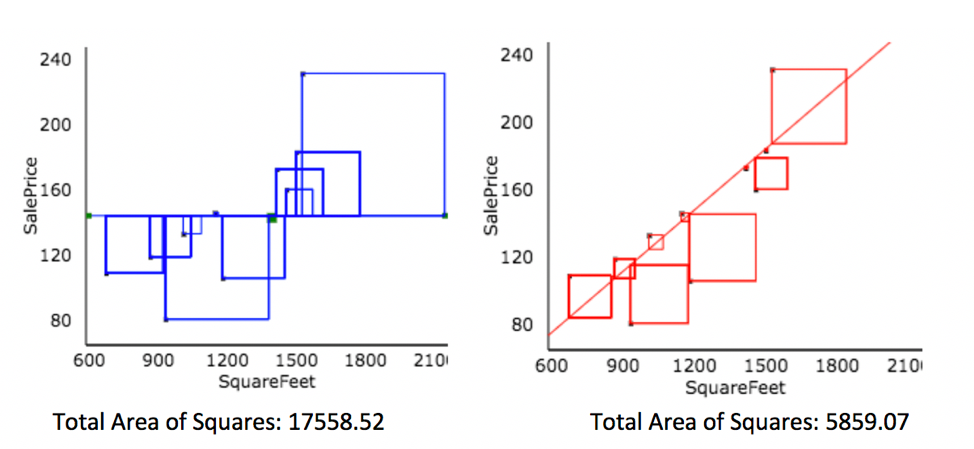
\includegraphics[width=0.65\linewidth]{Rsq}

Created at \url{http://www.rossmanchance.com/applets/RegShuffle.htm}.

\begin{itemize}
\item
  Blue Area = Total Variability (SST)
\item
  Red Area = Variability Remaining Unexplained by Model (SSR)
\item
  Blue Area - Red Area = Variability Explained by Model (SSM)
\item
  \(R^2 = \frac{\text{Area of Blue Squares} - \text{Area of Red Squares}}{\text{Area of Blue Squares}} = \frac{\text{SST}-\text{SSR}}{\text{SST}}= \frac{\text{SSM}}{\text{SST}}\)
\end{itemize}

\subsection{Variation Explained by SquareFeet
Model}\label{variation-explained-by-squarefeet-model-1}

\begin{itemize}
\item
  Total variability in house prices SST = 17,558.52\\
\item
  Variability remaining unexplained after accounting for square feet is
  SSR = 5,859.07\\
\item
  Variation explained by model accounting for square feet is
  \[ \text{SSM} = 17,558.52 - 5,859.07 = 11,699.45 \]
\item
  Proportion of variation explained by model accounting for square feet
  is \[ R^2=\frac{11,699.45}{17,558.52}\approx0.6663\]
\item
  66.6\% of the variation in house price is explained by the model using
  square feet as an explanatory variable.
\end{itemize}

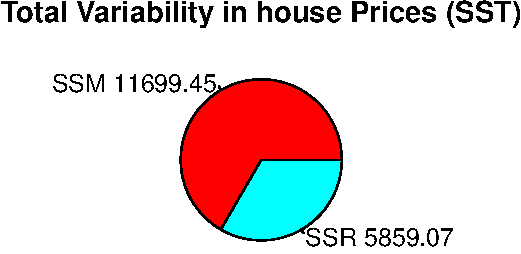
\includegraphics{_main_files/figure-latex/unnamed-chunk-56-1.pdf}

\subsection{Linear Correlation
Coefficient}\label{linear-correlation-coefficient}

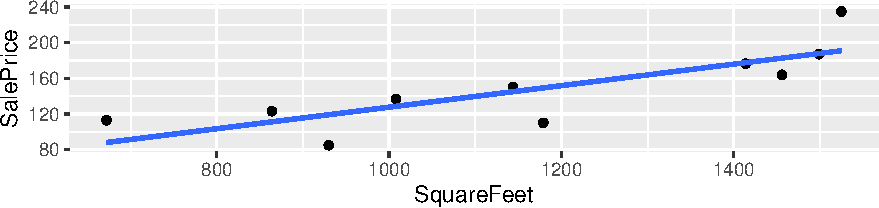
\includegraphics{_main_files/figure-latex/unnamed-chunk-57-1.pdf}

\begin{itemize}
\item
  For linear models with a single quantitative variable, the
  \textbf{linear correlation coefficient} \(r=\sqrt{R^2}\), or
  \(r=-\sqrt{R^2}\) (with sign matching the sign on the slope of the
  line), provides information about the strength and direction of the
  linear relationship between the variables.
\item
  \(-1 \leq r \leq 1\), and \(r\) close to \(\pm1\) provides evidence of
  strong linear relationship, while \(r\) close to 0 suggests linear
  relationship is weak.
\item
  \(r\) is only relevant for models with a single quantitative
  explanatory variable and a quantitative response variable, while
  \(R^2\) is relevant for any linear model with a quantitative response
  variable.
\end{itemize}

\begin{Shaded}
\begin{Highlighting}[]
\KeywordTok{cor}\NormalTok{(Houses}\OperatorTok{$}\NormalTok{SalePrice,Houses}\OperatorTok{$}\NormalTok{SquareFeet)}
\end{Highlighting}
\end{Shaded}

\begin{verbatim}
## [1] 0.8162794
\end{verbatim}

\section{Multiple Regression Model}\label{multiple-regression-model}

\subsection{Multiple Regression
Model}\label{multiple-regression-model-1}

Suppose we have information on both the neighborhood and square feet in
the houses. We can account for both of these together using a
\textbf{multiple regression model}, i.e.~a model with more than one
explanatory variable.

\begin{Shaded}
\begin{Highlighting}[]
\NormalTok{Houses}
\end{Highlighting}
\end{Shaded}

\begin{verbatim}
## # A tibble: 10 x 3
##    Neighborhood SquareFeet SalePrice
##    <fct>             <int>     <dbl>
##  1 NAmes               864     123  
##  2 CollgCr            1499     187  
##  3 NAmes              1414     176. 
##  4 Edwards             672     113  
##  5 CollgCr            1456     164. 
##  6 Edwards            1179     110  
##  7 Edwards             930      84.9
##  8 NAmes              1144     150  
##  9 CollgCr            1525     235  
## 10 NAmes              1008     137
\end{verbatim}

\subsection{2-Variable Model with Constant
Slope}\label{variable-model-with-constant-slope}

We'll assume the rate of increase wrt. square feet (i.e.~slope) is the
same in each neighborhood, but that some neighborhoods are more
expensive than others.

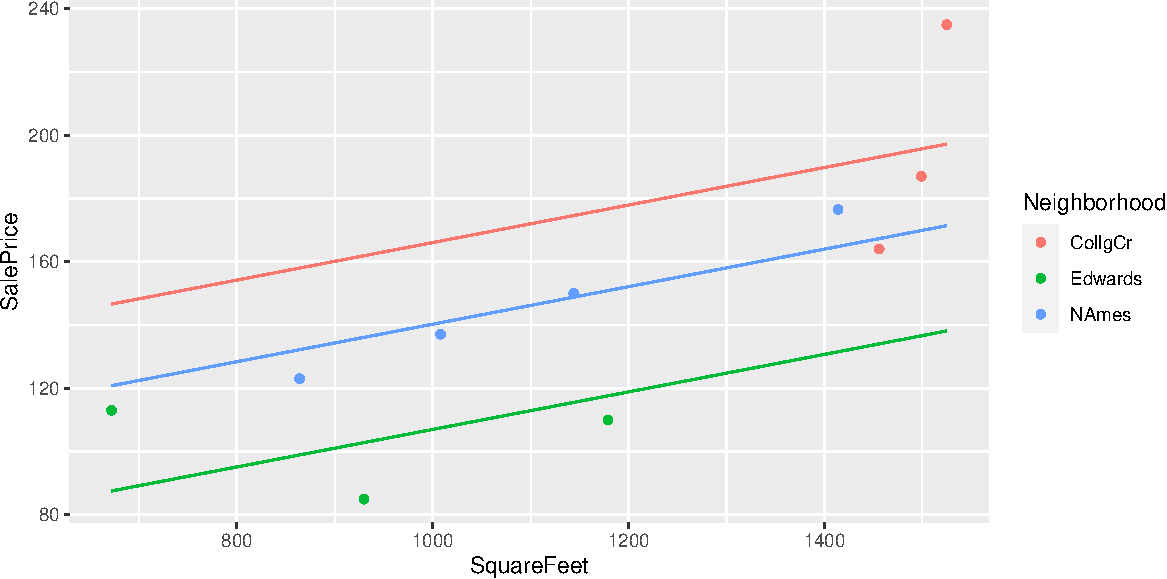
\includegraphics{_main_files/figure-latex/unnamed-chunk-61-1.pdf}

\subsection{House Price 2-Variable Model
Summary}\label{house-price-2-variable-model-summary}

\begin{Shaded}
\begin{Highlighting}[]
\NormalTok{M_Nbhd_SqFt <-}\StringTok{ }\KeywordTok{lm}\NormalTok{(}\DataTypeTok{data=}\NormalTok{Houses, SalePrice}\OperatorTok{~}\NormalTok{SquareFeet}\OperatorTok{+}\NormalTok{Neighborhood)}
\KeywordTok{summary}\NormalTok{(M_Nbhd_SqFt)}
\end{Highlighting}
\end{Shaded}

\begin{verbatim}
## 
## Call:
## lm(formula = SalePrice ~ SquareFeet + Neighborhood, data = Houses)
## 
## Residuals:
##     Min      1Q  Median      3Q     Max 
## -29.125  -9.050  -5.653   9.069  37.791 
## 
## Coefficients:
##                      Estimate Std. Error t value Pr(>|t|)
## (Intercept)         106.72593   68.92188   1.549    0.172
## SquareFeet            0.05933    0.04517   1.314    0.237
## NeighborhoodEdwards -59.09436   32.49761  -1.818    0.119
## NeighborhoodNAmes   -25.81232   25.59807  -1.008    0.352
## 
## Residual standard error: 24.55 on 6 degrees of freedom
## Multiple R-squared:  0.7941, Adjusted R-squared:  0.6911 
## F-statistic: 7.711 on 3 and 6 DF,  p-value: 0.01757
\end{verbatim}

\subsection{MR Model for SquareFeet and
Neighborhood}\label{mr-model-for-squarefeet-and-neighborhood}

In the model using both square feet and neighborhood, the regression
equation is

\(\widehat{\text{Price}}= b_0+ b_1 \times\text{SquareFeet}+ b_2\times\text{I}_{Edwards} + b_3 \times\text{I}_{NAmes}\)

\(\widehat{\text{Price}}= 106.73+ 0.06 \times\text{SquareFeet}+ -59.09 \times\text{I}_{Edwards} +-25.81 \times\text{I}_{NAmes}\)

\begin{itemize}
\tightlist
\item
  The intercept \(b_0\) represents the expected price of a house in
  College Creek with 0 square feet.

  \begin{itemize}
  \tightlist
  \item
    the intercept has no meaningful interpretation in this context
  \end{itemize}
\item
  \(b_1\) represents the expected change in price (in thousands) per
  one-unit increase in square feet, assuming neighborhood is the same.

  \begin{itemize}
  \tightlist
  \item
    on average, we expect the price of a house to increase by \$0.05933
    thousand (i.e. \$59.33) for each additional square foot, assuming
    the houses are in the same neighborhood.\\
  \end{itemize}
\item
  \(b_2\) and \(b_3\) represent the expected difference in price between
  a house in the Edwards (or North Ames) neighborhood, compared to the
  College Creek neighborhood, assuming square footage is the same.

  \begin{itemize}
  \tightlist
  \item
    We expect a house in the Edwards neighborhood to cost \$59.094 less
    than a house in the College Creek Neighborhood, assuming the houses
    are the same size.\\
  \item
    We expect a house in the North Ames Neighborhood to cost \$25.812
    less than a house in the College Creek Neighborhood, assuming the
    houses are the same size.
  \end{itemize}
\end{itemize}

\subsection{Predicting Price in MR
Model}\label{predicting-price-in-mr-model}

\(\widehat{\text{Price}}= 106.73+ 0.06 \times\text{SquareFeet}+ -59.09 \times\text{I}_{Edwards} +-25.81 \times\text{I}_{NAmes}\)

\begin{itemize}
\tightlist
\item
  848 square foot house in College Creek
\end{itemize}

\(\widehat{\text{Price}}= 106.73+ 0.06 \times848+ -59.09 \times0 +-25.81 \times 0 =157.0378\)
thousand

\begin{itemize}
\tightlist
\item
  1200 square foot house in North Ames
\end{itemize}

\(\widehat{\text{Price}}= 106.73+ 0.06 \times1200+ -59.09 \times0 +-25.81 \times1 = 152.1096\)
thousand

\begin{itemize}
\tightlist
\item
  2314 square foot house in Edwards
\end{itemize}

\(\widehat{\text{Price}}= 106.73+ 0.06 \times\text{SquareFeet}+ -59.09 \times1 +-25.81 \times 0 =184.9212\)
thousand

\subsection{Risk of Extrapolation}\label{risk-of-extrapolation}

Note that 2314 square feet is well outside the range of our observed
data. We should treat this prediction with caution, since we don't know
whether the trend we see in our data will continue.

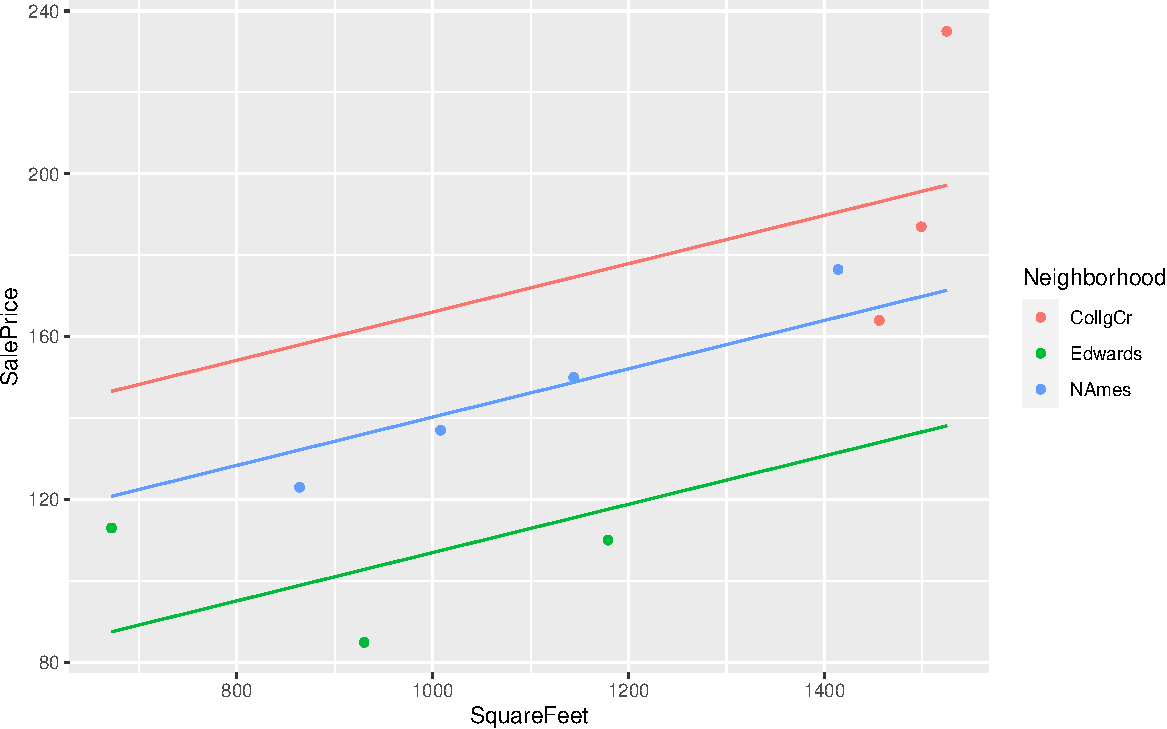
\includegraphics{_main_files/figure-latex/unnamed-chunk-64-1.pdf}

\subsection{Residuals for 2-Variable
Model}\label{residuals-for-2-variable-model}

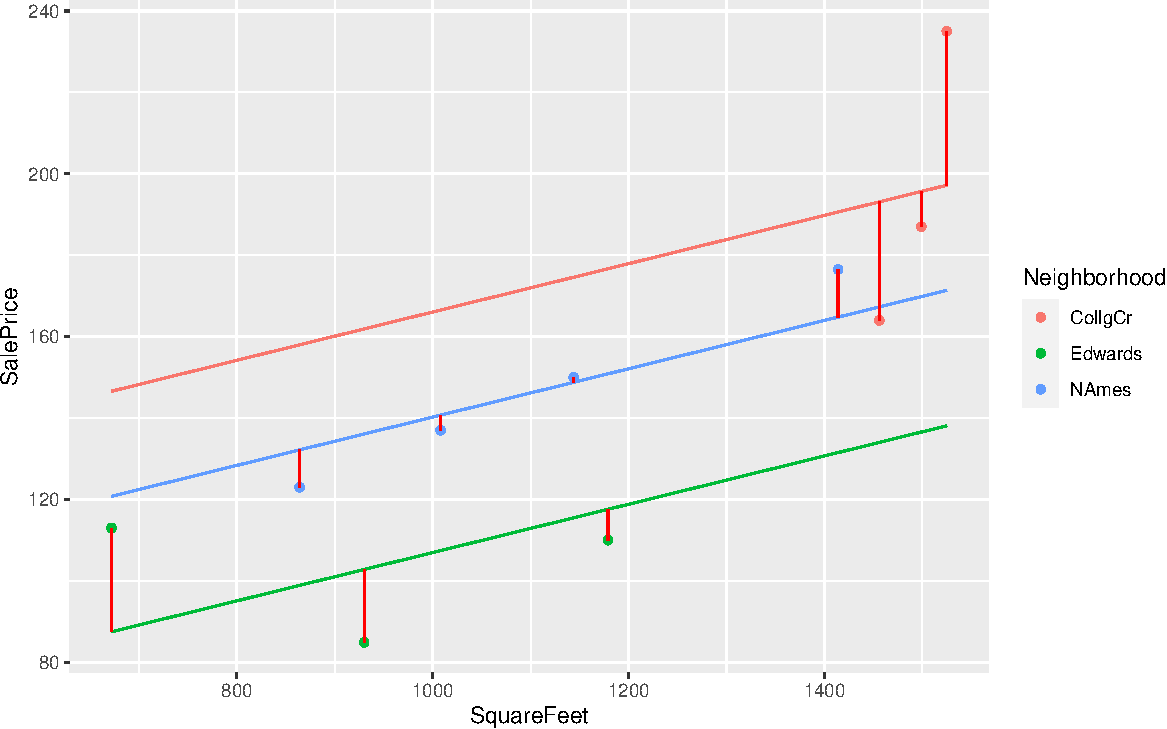
\includegraphics{_main_files/figure-latex/unnamed-chunk-65-1.pdf}

\subsection{Residuals for 2-Variable Model
(cont.)}\label{residuals-for-2-variable-model-cont.}

\begin{verbatim}
##    SalePrice Predicted   Residual  ResidualSq
## 1     123.00  132.1774  -9.177395   84.224570
## 2     187.00  195.6662  -8.666221   75.103383
## 3     176.50  164.8106  11.689410  136.642314
## 4     113.00   87.5034  25.496603  650.076744
## 5     163.99  193.1149 -29.124898  848.259699
## 6     110.00  117.5853  -7.585270   57.536321
## 7      84.90  102.8113 -17.911333  320.815835
## 8     150.00  148.7907   1.209343    1.462509
## 9     235.00  197.2089  37.791119 1428.168680
## 10    137.00  140.7214  -3.721358   13.848508
\end{verbatim}

\begin{Shaded}
\begin{Highlighting}[]
\KeywordTok{sum}\NormalTok{(M_Nbhd_SqFt}\OperatorTok{$}\NormalTok{residuals}\OperatorTok{^}\DecValTok{2}\NormalTok{)}
\end{Highlighting}
\end{Shaded}

\begin{verbatim}
## [1] 3616.139
\end{verbatim}

\subsection{Variation Explained by 2-Variable
Model}\label{variation-explained-by-2-variable-model}

\begin{itemize}
\item
  Total Variation in house prices: SST=17,558.52\\
\item
  Variation remaining unexplained after accounting for square feet is
  SSR=3,616.139\\
\item
  Variation explained by model accounting for square feet is
  \[SSM=SST-SSR=17,558.52 - 3,616.139 = 13,942.38\]
\item
  Proportion of variation in house prices explained by model is:
\end{itemize}

\[ R^2 = \frac{13,942.38}{17,558.52}\approx0.794 \]

\begin{itemize}
\tightlist
\item
  79.4\% of the variation in house price is explained by the model using
  square feet and neighborhood as an explanatory variables.
\end{itemize}

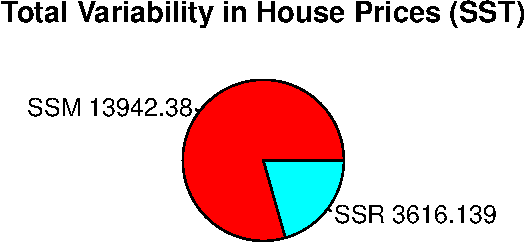
\includegraphics{_main_files/figure-latex/unnamed-chunk-68-1.pdf}

\subsection{Model Comparison Summary}\label{model-comparison-summary}

\begin{longtable}[]{@{}lllll@{}}
\toprule
Model & Variables & Unexplained Variability & Variability Explained &
\(R^2\)\tabularnewline
\midrule
\endhead
0 & None & 17558.52489 & 0 & 0\tabularnewline
1 & Nbhd & 4656.1875667 & 12902.3373233 & 0.734819\tabularnewline
2 & Sq. Ft. & 5859.0678887 & 11699.4570013 & 0.6663121\tabularnewline
3 & Nbhd, Sq. Ft. & 3616.1385638 & 13942.3863262 &
0.7940523\tabularnewline
\bottomrule
\end{longtable}

\textbf{Comments on \(R^2\):}

\begin{itemize}
\tightlist
\item
  \(R^2\) will never decrease when a new variable is added to a model.\\
\item
  This does not mean that adding more variables to a model always
  improves its ability to make predictions on new data.\\
\item
  \(R^2\) measures how well a model fits the data on which it was
  built.\\
\item
  It is possible for a model with high \(R^2\) to ``overfit'' the data
  it was built from, and thus perform poorly on new data. We will
  discuss this idea extensively later in the course.
\end{itemize}

\section{Least-Squares Estimation}\label{least-squares-estimation}

\subsection{Estimation of Model
Coefficients}\label{estimation-of-model-coefficients}

Learning Outcome:

\begin{enumerate}
\def\labelenumi{\arabic{enumi}.}
\tightlist
\item
  Explain how obtain model coefficients \(b_0, b_1, b_p\).
\end{enumerate}

\subsection{Least-Squares Estimation}\label{least-squares-estimation-1}

\begin{Shaded}
\begin{Highlighting}[]
\KeywordTok{ggplot}\NormalTok{(}\DataTypeTok{data=}\NormalTok{Houses, }\KeywordTok{aes}\NormalTok{(}\DataTypeTok{x=}\NormalTok{SquareFeet, }\DataTypeTok{y=}\NormalTok{SalePrice)) }\OperatorTok{+}\StringTok{ }\KeywordTok{geom_point}\NormalTok{() }\OperatorTok{+}\StringTok{ }
\StringTok{  }\KeywordTok{stat_smooth}\NormalTok{(}\DataTypeTok{method=}\StringTok{"lm"}\NormalTok{, }\DataTypeTok{se=}\OtherTok{FALSE}\NormalTok{)}
\end{Highlighting}
\end{Shaded}

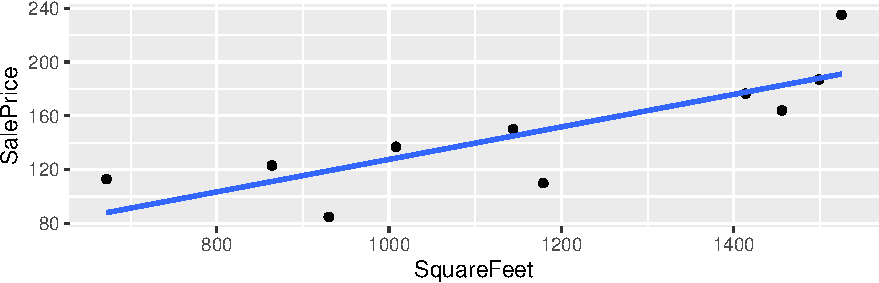
\includegraphics{_main_files/figure-latex/unnamed-chunk-70-1.pdf}

\begin{itemize}
\item
  The line \(\text{Price} = 6.82 + 0.12 \times \text{Square Feet}\) is
  considered the ``line of best fit'' in the sense that it minimizes the
  sum of the squared residuals.
\item
  This
  \href{http://www.rossmanchance.com/applets/RegShuffle.htm}{Rossman-Chance
  applet} provides an illustration of the line of best fit.
\end{itemize}

\subsection{Least Squares in General
Form}\label{least-squares-in-general-form}

Consider a dataset of \(n\) observations and p explanatory variables,

\[
\begin{bmatrix}
x_{11}    & x_{12}    & \cdots & x_{1p}  & y_1\\
x_{21}    & x_{22}    & \cdots & x_{2p} & y_2\\
\vdots    & \vdots    &  & \vdots  & \vdots\\
x_{n1}    & x_{n2}    & \cdots & x_{np} & y_n\\
\end{bmatrix}
\]

where \(y_i\) represents the response variable for case \(i\) and
\(x_{ip}\) represent the value or category indicatory of explanatory
variable \(p\) for case \(i\).

The line of best fit:
\(\hat{y}_i = b_0 + b_1x_{i1} + b_2{x_i2} + \ldots + b_px_{ip}\) is,
where \(b_0, b_1, \ldots, b_p\) are chosen to minimize:

\[ \displaystyle\sum_{i=1}^n (y_i -\hat{y}_i)^2  = \displaystyle\sum_{i=1}^n (y_i - (b_0 + b_1x_{i1} + b_2{x_i2} + \ldots + b_px_{ip}))^2 \]

\subsection{Least-Squares Estimation in Simple Linear
Regression}\label{least-squares-estimation-in-simple-linear-regression}

\begin{itemize}
\item
  Consider a \textbf{simple linear regression(SLR)} model, which is one
  with a singe quantitative explanatory variable.
\item
  \(\hat{y}_i = b_0+b_1x_i\)
\item
  we need to minimize:
\end{itemize}

\[
\displaystyle\sum_{i=1}^n(y_i-\hat{y}_i)^2 =\displaystyle\sum_{i=1}^n(y_i-(b_0+b_1x_i))^2
\]

\subsection{Least-Squares Estimation in Simple Linear Regression
(cont.)}\label{least-squares-estimation-in-simple-linear-regression-cont.}

Using calculus, it can be shown that this quantity is minimized when

\begin{itemize}
\item
  \(b_1=\frac{\displaystyle\sum_{i=1}^{n}(x_i-\bar{x})(y_i-\bar{y})}{\displaystyle\sum_{i=1}^{n}(x_i-\bar{x})^2}=\frac{\displaystyle\sum_{i=1}^{n} x_i y_i-\frac{\displaystyle\sum_{i=1}^{n} x_i \displaystyle\sum_{i=1}^{n} y_i }{n}}{\left(\displaystyle\sum_{i=1}^{n} x_i^2 -\frac{\left(\displaystyle\sum_{i=1}^{n} x_i\right)^2}{n}\right)}\)
\item
  \(b_0=\bar{y}-b_1\bar{x}\) (where
  \(\bar{y}=\frac{\displaystyle\sum_{i=1}^{n}{y_i}}{n}\), and
  \(\bar{x}=\frac{\displaystyle\sum_{i=1}^{n}{x_i}}{n}\)).
\end{itemize}

\subsection{LS Estimation for One Categorical
Variable}\label{ls-estimation-for-one-categorical-variable}

\begin{itemize}
\item
  Consider a model with a single categorical variable (such as
  neighborhood), with G+1 categories, numbered \(g=0,2, \ldots, G\)
\item
  Then \(\hat{y}_i = b_0 + b_1x_{i1} + \ldots +b_{G}x_{iG}\).
\item
  we need to minimize
\end{itemize}

\[
\displaystyle\sum_{i=1}^n(y_i-\hat{y}_i)^2 =\displaystyle\sum_{i=1}^n(y_i-(b_0 + b_1x_{i1} + \ldots +b_{G}x_{iG}))^2.   
\]

\begin{itemize}
\tightlist
\item
  It can be shown that this is achieved when\\
\item
  \(b_0 = \bar{y_0}\) (i.e.~the average response in the ``baseline
  group''), and\\
\item
  \(b_j = \bar{y_j} - \bar{y}_0\)
\end{itemize}

\subsection{LS Estimation More
Generally}\label{ls-estimation-more-generally}

\begin{itemize}
\tightlist
\item
  For multiple regression models, the logic is the same. We need to
  choose \(b_0, b_1, \ldots, b_p\) in order to minimize
\end{itemize}

\[ \displaystyle\sum_{i=1}^n (y_i -\hat{y}_i)^2  = \displaystyle\sum_{i=1}^n (y_i -(b_0 + b_1x_{i1} + b_2{x_i2} + \ldots + b_px_{ip}))^2 \]

\begin{itemize}
\item
  The mathematics, however are more complicated and require inverting a
  matrix. This goes beyond the scope of this class, so we will let R do
  the estimation and use the results.
\item
  More on least squares estimation in multiple regression can be found
  \href{http://www.math.chalmers.se/Stat/Grundutb/GU/MSG500/A10/lecture5.pdf}{here}.
\end{itemize}

\section{ANalysis Of VAriance}\label{analysis-of-variance}

\subsection{ANalysis Of VAriance}\label{analysis-of-variance-1}

Learning Outcomes

\begin{enumerate}
\def\labelenumi{\arabic{enumi}.}
\tightlist
\item
  Use ANOVA F-statistics to compare models and sub-models.\\
\item
  Use F-statistics to measure variability between groups, compared to
  variability within groups.
\end{enumerate}

\subsection{Comparing Submodels}\label{comparing-submodels}

\begin{longtable}[]{@{}lllll@{}}
\toprule
Model & Variables & Unexplained Variability & Variability Explained &
\(R^2\)\tabularnewline
\midrule
\endhead
0 & None & 17558.52489 & 0 & 0\tabularnewline
1 & Nbhd. & 4656.1875667 & 12902.3373233 & 0.734819\tabularnewline
2 & Sq. Ft & 5859.0678887 & 11699.4570013 & 0.6663121\tabularnewline
3 & Nbhd, Sq. Ft. & 3616.1385638 & 13942.3863262 &
0.7940523\tabularnewline
\bottomrule
\end{longtable}

\begin{itemize}
\item
  Notice that Model 1 is a submodel of Model 3, since all variables used
  in Model 1 are also used in Model 3.
\item
  Model 2 is also a submodel of Model 3.
\item
  Model 0 is a submodel of Models 1, 2, and 3.
\item
  Models 1 and 2 are not submodels of each other, since Model 1 contains
  a variable used in Model 2 and Model 2 contains a variable not used in
  Model 1.
\end{itemize}

\subsection{Comparison of Sub-Models}\label{comparison-of-sub-models}

When one model is a submodel of another, we can compare the amount of
variability explained by the models, using a technique known as
\textbf{ANalysis Of VAriance (ANOVA)}.

Reduced Model:
\(\hat{y}_i = b_0 + b_1x_{i1} + b_2{x_i2} + \ldots + b_qx_{iq}\)

Full Model:
\(\hat{y}_i = b_0 + b_1x_{i1} + b_2{x_i2} + \ldots + b_qx_{iq} + b_{q+1}x_{i{q+1}} \ldots + b_px_{ip}\)

p = \#\# variables in Full Model\\
q = \#\# variables in Reduced Model\\
n = number of observations

We calculate a statistic called F:

\[
\begin{aligned}
F  &=\frac{\frac{\text{Unexplained Variability in Reduced Model}-\text{Unexplained Variability in Full Model}}{p-q}}{\frac{\text{Unexplained Variability in Full Model}}{n-(p+1)}} \\
&= \frac{\frac{\text{SSR}_{\text{Reduced}}-\text{SSR}_{\text{Full}}}{p-q}}{\frac{\text{SSR}_{\text{Full}}}{n-(p+1)}}
\end{aligned}
\]

\subsection{Comments on F-Statistic}\label{comments-on-f-statistic}

\begin{itemize}
\item
  The F-statistic measures the amount of variability explained by adding
  additional variable(s) to the model, relative to the total amount of
  unexplained variability.
\item
  Large values of F indicate that adding the additional explanatory
  variables is helpful in explaining variability in the response
  variable\\
\item
  Small values of F indicate that adding new explanatory variables
  variables does not make much of a difference in explaining variability
  in the response variable\\
\item
  What counts as ``large'' is depends on \(n, p,\) and \(q\). We will
  revisit this later in the course.
\end{itemize}

\subsection{ANOVA F-Statistic}\label{anova-f-statistic}

Let's Calculate an ANOVA F-Statistic to compare Models 2 and 3.

Reduced Model:
\(\widehat{\text{Price}}= b_0+ b_1 \times\text{SquareFeet}\)

Full Model:
\(\widehat{\text{Price}}= b_0+ b_1 \times\text{SquareFeet}+ b_2\times\text{I}_{Edwards} + b_3 \times\text{I}_{NAmes}\)

\[
\begin{aligned}
F &= \frac{\frac{\text{SSR}_{\text{Reduced}}-\text{SSR}_{\text{Full}}}{p-q}}{\frac{\text{SSR}_{\text{Full}}}{n-(p+1)}} \\
&=\frac{\frac{5,859.07-3,616.14}{3-1}}{\frac{3,616.13}{10-(3+1)}} \\
\end{aligned}
\]

\begin{Shaded}
\begin{Highlighting}[]
\NormalTok{SSR2 <-}\StringTok{ }\KeywordTok{sum}\NormalTok{(M_SqFt}\OperatorTok{$}\NormalTok{residuals}\OperatorTok{^}\DecValTok{2}\NormalTok{); SSR3 <-}\StringTok{ }\KeywordTok{sum}\NormalTok{(M_Nbhd_SqFt}\OperatorTok{$}\NormalTok{residuals}\OperatorTok{^}\DecValTok{2}\NormalTok{);}
\NormalTok{((SSR2}\OperatorTok{-}\NormalTok{SSR3)}\OperatorTok{/}\NormalTok{(}\DecValTok{3}\OperatorTok{-}\DecValTok{1}\NormalTok{))}\OperatorTok{/}\NormalTok{((SSR3)}\OperatorTok{/}\NormalTok{(}\DecValTok{10}\OperatorTok{-}\NormalTok{(}\DecValTok{3}\OperatorTok{+}\DecValTok{1}\NormalTok{)))}
\end{Highlighting}
\end{Shaded}

\begin{verbatim}
## [1] 1.860766
\end{verbatim}

\subsection{ANOVA F-Statistic for M2 vs M3 in
R}\label{anova-f-statistic-for-m2-vs-m3-in-r}

\begin{Shaded}
\begin{Highlighting}[]
\KeywordTok{anova}\NormalTok{(M_SqFt, M_Nbhd_SqFt)}
\end{Highlighting}
\end{Shaded}

\begin{verbatim}
## Analysis of Variance Table
## 
## Model 1: SalePrice ~ SquareFeet
## Model 2: SalePrice ~ SquareFeet + Neighborhood
##   Res.Df    RSS Df Sum of Sq      F Pr(>F)
## 1      8 5859.1                           
## 2      6 3616.1  2    2242.9 1.8608 0.2351
\end{verbatim}

Notice the F-statistic has the same value.

Later, we will examine what this tells us about adding Neighborhood to a
model already containing square feet as an explanatory variable.

\subsection{ANOVA F-Statistic for M1 vs
M0}\label{anova-f-statistic-for-m1-vs-m0}

Now, let's compare Models 0 and 1.

Reduced Model: \(\widehat{\text{Price}}_i = b_0\)

Full Model:
\(\widehat{\text{Price}}_i = b_0 + b_1\text{I}_{\text{Edwards}} + b_2\text{I}_{\text{NAmes}}\)

\[
\begin{aligned}
F &= \frac{\frac{\text{SSR}_{\text{Reduced}}-\text{SSR}_{\text{Full}}}{p-q}}{\frac{\text{SSR}_{\text{Full}}}{n-(p+1)}} \\
&=\frac{\frac{17558.52-4656.19}{2-0}}{\frac{4656.19}{10-(2+1)}}
\end{aligned}
\]

\begin{Shaded}
\begin{Highlighting}[]
\NormalTok{SSR0 <-}\StringTok{ }\KeywordTok{sum}\NormalTok{(M0}\OperatorTok{$}\NormalTok{residuals}\OperatorTok{^}\DecValTok{2}\NormalTok{); SSR1 <-}\StringTok{ }\KeywordTok{sum}\NormalTok{(M_Nbhd}\OperatorTok{$}\NormalTok{residuals}\OperatorTok{^}\DecValTok{2}\NormalTok{);}
\NormalTok{((SSR0}\OperatorTok{-}\NormalTok{SSR1)}\OperatorTok{/}\NormalTok{(}\DecValTok{2}\OperatorTok{-}\DecValTok{0}\NormalTok{))}\OperatorTok{/}\NormalTok{((SSR1)}\OperatorTok{/}\NormalTok{(}\DecValTok{10}\OperatorTok{-}\NormalTok{(}\DecValTok{2}\OperatorTok{+}\DecValTok{1}\NormalTok{)))}
\end{Highlighting}
\end{Shaded}

\begin{verbatim}
## [1] 9.698531
\end{verbatim}

\subsection{ANOVA F-Statistic for M0 vs M1 in
R}\label{anova-f-statistic-for-m0-vs-m1-in-r}

\begin{Shaded}
\begin{Highlighting}[]
\KeywordTok{anova}\NormalTok{(M0, M_Nbhd)}
\end{Highlighting}
\end{Shaded}

\begin{verbatim}
## Analysis of Variance Table
## 
## Model 1: SalePrice ~ 1
## Model 2: SalePrice ~ Neighborhood
##   Res.Df     RSS Df Sum of Sq      F   Pr(>F)   
## 1      9 17558.5                                
## 2      7  4656.2  2     12902 9.6985 0.009603 **
## ---
## Signif. codes:  0 '***' 0.001 '**' 0.01 '*' 0.05 '.' 0.1 ' ' 1
\end{verbatim}

\subsection{ANOVA F-Statistic for Categorical
Variables}\label{anova-f-statistic-for-categorical-variables}

\begin{itemize}
\tightlist
\item
  The difference between M1 and M0 is that M1 considers the house's
  neighborhood, while M0 does not.\\
\item
  If neighborhood is helpful in modeling house price, then we would
  expect to see a high F-statistic.\\
\item
  Another way to think about this is that if the amount of variability
  in house prices between different neighborhoods is large, relative to
  the amount of variability within neighborhoods, then the F-statistic
  should be large.\\
\item
  In fact, an alternative (an mathematically equivalent) way to
  calculate the F-statistic is to calculate the ratio of variability
  between different neighborhoods, relative to the amount of variability
  within neighborhoods.
\end{itemize}

\subsection{F-Statistic for Categorical Variables
Illustration}\label{f-statistic-for-categorical-variables-illustration}

An F-statistic compares the amount of variability between groups to the
amount of variability within groups.

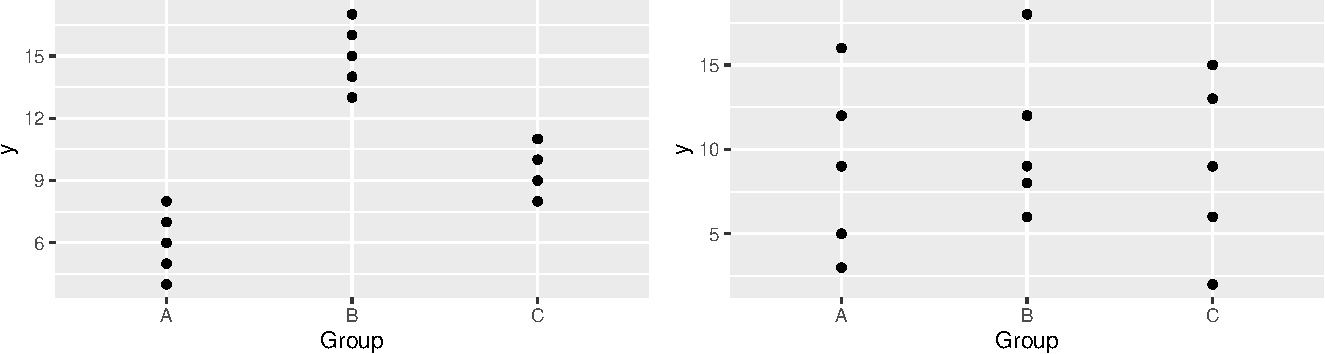
\includegraphics{_main_files/figure-latex/unnamed-chunk-76-1.pdf}

\begin{longtable}[]{@{}lll@{}}
\toprule
& Scenario 1 & Scenario 2\tabularnewline
\midrule
\endhead
variation between groups & High & Low\tabularnewline
variation within groups & Low & High\tabularnewline
F Statistic & Large & Small\tabularnewline
Result & Evidence of Group Differences & No evidence of
differences\tabularnewline
\bottomrule
\end{longtable}

\subsection{Alternative F-Statistic
Formula}\label{alternative-f-statistic-formula}

For a categorical variable with \(g\) groups,

\begin{itemize}
\item
  let \(\bar{y}_{1\cdot}, \ldots, \bar{y}_{g\cdot}\) represent the mean
  response for each group.
\item
  let \(n_1, \ldots, n_g\) represent the sample size for each group
\item
  Then
  \(\frac{\displaystyle\sum_{i=1}^g\sum_{j=1}^{n_i}n_i(y_{i\cdot}-\bar{y}_{\cdot\cdot})^2}{g-1}\)
  gives a measure of how much the group means differ, and
\item
  \(\frac{\displaystyle\sum_{i=1}^g\sum_{j=1}^{n_i}(y_{ij}-\bar{y}_{i\cdot})^2}{n-g}\)
  gives a measure of how much individual observations differ within
  groups
\end{itemize}

\subsection{Alternative F-Statistic Formula
(cont.)}\label{alternative-f-statistic-formula-cont.}

\begin{itemize}
\tightlist
\item
  An alternative formula for this F-statistic is:
\end{itemize}

\[
F= \frac{\text{Variability between Neighborhoods}}{\text{Variability within Neighborhoods}}= \frac{\frac{\displaystyle\sum_{i=1}^g\sum_{j=1}^{n_i}n_i(y_{i\cdot}-\bar{y}_{\cdot\cdot})^2}{g-1}}{\frac{\displaystyle\sum_{i=1}^g\sum_{j=1}^{n_i}(y_{ij}-\bar{y}_{i\cdot})^2}{n-g}}
\]

\begin{itemize}
\tightlist
\item
  It can be shown that this statistic is equivalent to the one we saw
  previously.
\end{itemize}

\subsection{Calculating F-Statistic for Categorical
Variables}\label{calculating-f-statistic-for-categorical-variables}

We have seen previously that:

\begin{itemize}
\tightlist
\item
  \(\bar{y}_{\cdot\cdot}=148.039\) (overall average price), and \(n=10\)
\item
  \(\bar{y}_{1\cdot}=195.330\) (average price in College Creek), and
  \(n_1=3\)\\
\item
  \(\bar{y}_{2\cdot}=102.633\) (average price in Edwards), and
  \(n_2=4\)\\
\item
  \(\bar{y}_{3\cdot}=146.625\) (average price in North Ames), and
  \(n_3=3\)
\end{itemize}

Then,

\begin{itemize}
\item
  \(\frac{\displaystyle\sum_{i=1}^g\sum_{j=1}^{n_i}(y_{i\cdot}-\bar{y}_{\cdot\cdot})^2}{g-1} = \frac{3(195.330-148.039)^2+3(102.633-148.039)^2+4(146.625-148.039)^2}{3-1} = \frac{12902}{2}\),
  and
\item
  \(\frac{\displaystyle\sum_{i=1}^g\sum_{j=1}^{n_i}(y_{ij}-\bar{y}_{i\cdot})^2}{n-g} = \frac{(123.00-146.625)^2+ (187.00 - 195.33)^2 + \ldots + (137.00-146.625)^2}{10-3} = \frac{4656}{7}\)
\end{itemize}

\subsection{Calculating F-Statistic for Categorical
Variables}\label{calculating-f-statistic-for-categorical-variables-1}

\[
F= \frac{\frac{\displaystyle\sum_{i=1}^g\sum_{j=1}^{n_i}n_i(y_{i\cdot}-\bar{y}_{\cdot\cdot})^2}{g-1}}{\frac{\displaystyle\sum_{i=1}^g\sum_{j=1}^{n_i}(y_{ij}-\bar{y}_{i\cdot})^2}{n-g}} = \frac{\frac{(195.330-148.039)^2+(102.633-148.039)^2+(146.625-148.039)^2}{3-1}}{\frac{(123.00-146.625)^2+ (187.00 - 195.33)^2 + \ldots + (137.00-146.625)^2}{10-3}} = \frac{\frac{12902}{2}}{\frac{4656}{7}}
\]

\begin{itemize}
\tightlist
\item
  Note that the quantity in the the quantity in the third line is
  equivalent to the sum of the squared residuals using M2. Thus, we can
  calculate F using:
\end{itemize}

\begin{Shaded}
\begin{Highlighting}[]
\NormalTok{((}\DecValTok{3}\OperatorTok{*}\NormalTok{(}\FloatTok{195.330}\OperatorTok{-}\FloatTok{148.039}\NormalTok{)}\OperatorTok{^}\DecValTok{2}\OperatorTok{+}\DecValTok{3}\OperatorTok{*}\NormalTok{(}\FloatTok{102.633}\OperatorTok{-}\FloatTok{148.039}\NormalTok{)}\OperatorTok{^}\DecValTok{2}\OperatorTok{+}\DecValTok{4}\OperatorTok{*}\NormalTok{(}\FloatTok{146.625}\OperatorTok{-}\FloatTok{148.039}\NormalTok{)}\OperatorTok{^}\DecValTok{2}\NormalTok{)}\OperatorTok{/}\NormalTok{(}\DecValTok{3}\OperatorTok{-}\DecValTok{1}\NormalTok{))}\OperatorTok{/}\NormalTok{(}\KeywordTok{sum}\NormalTok{(M_Nbhd}\OperatorTok{$}\NormalTok{residuals}\OperatorTok{^}\DecValTok{2}\NormalTok{)}\OperatorTok{/}\NormalTok{(}\DecValTok{10}\OperatorTok{-}\DecValTok{3}\NormalTok{))}
\end{Highlighting}
\end{Shaded}

\begin{verbatim}
## [1] 9.6986
\end{verbatim}

\subsection{Alternative Calculation in
R}\label{alternative-calculation-in-r}

This interpretation of the F-statistic can be seen using the AOV command
in R.

\begin{Shaded}
\begin{Highlighting}[]
\NormalTok{AOV_Nbhd <-}\StringTok{ }\KeywordTok{aov}\NormalTok{(}\DataTypeTok{data=}\NormalTok{Houses, SalePrice}\OperatorTok{~}\NormalTok{Neighborhood)}
\KeywordTok{summary}\NormalTok{(AOV_Nbhd)}
\end{Highlighting}
\end{Shaded}

\begin{verbatim}
##              Df Sum Sq Mean Sq F value Pr(>F)   
## Neighborhood  2  12902    6451   9.699 0.0096 **
## Residuals     7   4656     665                  
## ---
## Signif. codes:  0 '***' 0.001 '**' 0.01 '*' 0.05 '.' 0.1 ' ' 1
\end{verbatim}

\begin{itemize}
\item
  The \emph{Neighborhood} line represents the variability between
  neighborhoods\\
\item
  The \emph{Residuals} line represents the variability within
  neighborhoods
\item
  The first two columns give the quantities we use in our formula. The
  third column, representing the ratio of the first two columns is
  called a \textbf{mean square.}
\end{itemize}

\subsection{F-Statistic in R Output}\label{f-statistic-in-r-output}

The last line in the summary output includes the F-statistic for the
specified model, compared to a reduced model that includes only the
intercept.

Reduced Model: \(\widehat{Y}= b_0\)

Full Model: \(\widehat{Y}= b_0+ b_1 X_{i1}+ \ldots+ b_p X_{ip}\)

This statistic addresses the question \emph{``Do any of the explanatory
variables help explain variability in Y?''}.

When there is only one explanatory variable in the model, this statistic
can be used to test whether there is evidence that this statistic is
associated with \(Y\).

\subsection{F-Statistic in R Output
M1}\label{f-statistic-in-r-output-m1}

The F-statistic compares a full model that includes neighborhood to a
reduced model that predicts each price using the overall average.

\begin{Shaded}
\begin{Highlighting}[]
\KeywordTok{summary}\NormalTok{(M_Nbhd)}
\end{Highlighting}
\end{Shaded}

\begin{verbatim}
## 
## Call:
## lm(formula = SalePrice ~ Neighborhood, data = Houses)
## 
## Residuals:
##     Min      1Q  Median      3Q     Max 
## -31.340 -15.706  -2.477   9.617  39.670 
## 
## Coefficients:
##                     Estimate Std. Error t value   Pr(>|t|)    
## (Intercept)           195.33      14.89  13.118 0.00000349 ***
## NeighborhoodEdwards   -92.70      21.06  -4.402    0.00315 ** 
## NeighborhoodNAmes     -48.71      19.70  -2.473    0.04267 *  
## ---
## Signif. codes:  0 '***' 0.001 '**' 0.01 '*' 0.05 '.' 0.1 ' ' 1
## 
## Residual standard error: 25.79 on 7 degrees of freedom
## Multiple R-squared:  0.7348, Adjusted R-squared:  0.6591 
## F-statistic: 9.699 on 2 and 7 DF,  p-value: 0.009603
\end{verbatim}

\subsection{F-Statistic in R Output
M2}\label{f-statistic-in-r-output-m2}

The F-statistic compares a full model that includes square feet to a
reduced model that predicts each price using the overall average.

\begin{Shaded}
\begin{Highlighting}[]
\KeywordTok{summary}\NormalTok{(M_SqFt)}
\end{Highlighting}
\end{Shaded}

\begin{verbatim}
## 
## Call:
## lm(formula = SalePrice ~ SquareFeet, data = Houses)
## 
## Residuals:
##     Min      1Q  Median      3Q     Max 
## -39.235 -14.309   2.052  10.966  43.971 
## 
## Coefficients:
##             Estimate Std. Error t value Pr(>|t|)   
## (Intercept)  6.82000   36.35455   0.188  0.85586   
## SquareFeet   0.12079    0.03022   3.997  0.00397 **
## ---
## Signif. codes:  0 '***' 0.001 '**' 0.01 '*' 0.05 '.' 0.1 ' ' 1
## 
## Residual standard error: 27.06 on 8 degrees of freedom
## Multiple R-squared:  0.6663, Adjusted R-squared:  0.6246 
## F-statistic: 15.97 on 1 and 8 DF,  p-value: 0.003967
\end{verbatim}

\subsection{F-Statistic in R Output
M3}\label{f-statistic-in-r-output-m3}

The F-statistic compares a full model that includes square feet and
neighborhood to a reduced model that predicts each price using only the
overall average.

\begin{Shaded}
\begin{Highlighting}[]
\KeywordTok{summary}\NormalTok{(M_Nbhd_SqFt)}
\end{Highlighting}
\end{Shaded}

\begin{verbatim}
## 
## Call:
## lm(formula = SalePrice ~ SquareFeet + Neighborhood, data = Houses)
## 
## Residuals:
##     Min      1Q  Median      3Q     Max 
## -29.125  -9.050  -5.653   9.069  37.791 
## 
## Coefficients:
##                      Estimate Std. Error t value Pr(>|t|)
## (Intercept)         106.72593   68.92188   1.549    0.172
## SquareFeet            0.05933    0.04517   1.314    0.237
## NeighborhoodEdwards -59.09436   32.49761  -1.818    0.119
## NeighborhoodNAmes   -25.81232   25.59807  -1.008    0.352
## 
## Residual standard error: 24.55 on 6 degrees of freedom
## Multiple R-squared:  0.7941, Adjusted R-squared:  0.6911 
## F-statistic: 7.711 on 3 and 6 DF,  p-value: 0.01757
\end{verbatim}

\subsection{When to Use F-Statistics for Model
Comparison}\label{when-to-use-f-statistics-for-model-comparison}

\begin{itemize}
\tightlist
\item
  We have used F-statistics to compare models 1 and 3, and models 0 and
  2.
\item
  We could also calculate F-statistics comparing models 2 and 3, models
  0 and 1, and models 0 and 3.\\
\item
  We cannot use an F-statistic to compare models 1 and 2, since neither
  is a submodel of the other.\\
\item
  When comparing a model to the ``intercept-only'' model, we can use the
  model summary output. When comparing other to other submodels, use the
  \texttt{aov()} or \texttt{anova()} commands.
\end{itemize}

\subsection{Interaction Models with Categorical
Variables}\label{interaction-models-with-categorical-variables}

Learning Outcomes

\begin{enumerate}
\def\labelenumi{\arabic{enumi}.}
\tightlist
\item
  Fit models involving interactions.
\item
  Make interpret regression coefficients for models with interactions.\\
\item
  Compare and contrast the assumptions behind models with and without
  interaction terms.
\end{enumerate}

\begin{itemize}
\tightlist
\item
  We will build a model to predict the weight of a bear, using other
  characteristics including season, sex, and age.
\end{itemize}

\section{Interaction Models with Categorical
Variables}\label{interaction-models-with-categorical-variables-1}

\subsection{Bear Data}\label{bear-data}

Data are available in the \texttt{Bolstad} R package. We examine the
structure of the dataset.

\begin{Shaded}
\begin{Highlighting}[]
\KeywordTok{library}\NormalTok{(Bolstad)}
\KeywordTok{data}\NormalTok{(bears)}
\KeywordTok{glimpse}\NormalTok{(bears)}
\end{Highlighting}
\end{Shaded}

\begin{verbatim}
## Rows: 143
## Columns: 12
## $ ID      <int> 39, 41, 41, 41, 41, 43, 43, 45, 45, 48, 69, 83, 83, 83, 83, 91~
## $ Age     <int> 19, 19, 20, 23, 29, 19, 20, 55, 67, 81, NA, 115, 117, 124, 140~
## $ Month   <int> 7, 7, 8, 11, 5, 7, 8, 7, 7, 9, 10, 7, 9, 4, 8, 8, 4, 9, 7, 4, ~
## $ Sex     <int> 1, 2, 2, 2, 2, 1, 1, 1, 1, 1, 1, 1, 1, 1, 1, 2, 2, 1, 1, 1, 1,~
## $ Head.L  <dbl> 10.0, 11.0, 12.0, 12.5, 12.0, 11.0, 12.0, 16.5, 16.5, 15.5, 16~
## $ Head.W  <dbl> 5.0, 6.5, 6.0, 5.0, 6.0, 5.5, 5.5, 9.0, 9.0, 8.0, 8.0, 10.0, 7~
## $ Neck.G  <dbl> 15.0, 20.0, 17.0, 20.5, 18.0, 16.0, 17.0, 28.0, 27.0, 31.0, 32~
## $ Length  <dbl> 45.0, 47.5, 57.0, 59.5, 62.0, 53.0, 56.0, 67.5, 78.0, 72.0, 77~
## $ Chest.G <dbl> 23.0, 24.0, 27.0, 38.0, 31.0, 26.0, 30.5, 45.0, 49.0, 54.0, 52~
## $ Weight  <int> 65, 70, 74, 142, 121, 80, 108, 344, 371, 416, 432, 348, 476, 4~
## $ Obs.No  <int> 1, 1, 2, 3, 4, 1, 2, 1, 2, 1, 1, 1, 2, 3, 4, 1, 1, 2, 1, 1, 2,~
## $ Name    <fct> Allen, Berta, Berta, Berta, Berta, Clyde, Clyde, Doc, Doc, Qui~
\end{verbatim}

\subsection{Bears Data Cleaning}\label{bears-data-cleaning}

Notice that we have multiple observations on the same bears. The
procedures we have learned so far require observations to be independent
of each other. Thus, we'll keep only the first observation on each bear.

\begin{Shaded}
\begin{Highlighting}[]
\NormalTok{Bears_Subset <-}\StringTok{ }\NormalTok{bears }\OperatorTok\StringTok{ }\KeywordTok{filter}\NormalTok{(Obs.No }\OperatorTok{==}\StringTok{ }\DecValTok{1}\NormalTok{)}
\end{Highlighting}
\end{Shaded}

The variables Month and Sex are coded as integers, but it really makes
more sense to think of these as categorical variables. Thus, we will
convert them to factors.

\begin{Shaded}
\begin{Highlighting}[]
\NormalTok{Bears_Subset}\OperatorTok{$}\NormalTok{Month <-}\StringTok{ }\KeywordTok{as.factor}\NormalTok{(Bears_Subset}\OperatorTok{$}\NormalTok{Month)}
\NormalTok{Bears_Subset}\OperatorTok{$}\NormalTok{Sex <-}\StringTok{ }\KeywordTok{as.factor}\NormalTok{(Bears_Subset}\OperatorTok{$}\NormalTok{Sex)}
\end{Highlighting}
\end{Shaded}

\subsection{Examining the Subset}\label{examining-the-subset}

\begin{Shaded}
\begin{Highlighting}[]
\KeywordTok{glimpse}\NormalTok{(Bears_Subset)}
\end{Highlighting}
\end{Shaded}

\begin{verbatim}
## Rows: 97
## Columns: 12
## $ ID      <int> 39, 41, 43, 45, 48, 69, 83, 91, 179, 241, 253, 274, 280, 394, ~
## $ Age     <int> 19, 19, 19, 55, 81, NA, 115, 104, 100, 56, 51, 57, 53, NA, 68,~
## $ Month   <fct> 7, 7, 7, 7, 9, 10, 7, 8, 4, 7, 4, 9, 5, 6, 8, 8, 8, 8, 8, 8, 9~
## $ Sex     <fct> 1, 2, 1, 1, 1, 1, 1, 2, 2, 1, 1, 2, 2, 1, 1, 1, 2, 1, 2, 1, 1,~
## $ Head.L  <dbl> 10.0, 11.0, 11.0, 16.5, 15.5, 16.0, 17.0, 15.5, 13.0, 15.0, 13~
## $ Head.W  <dbl> 5.0, 6.5, 5.5, 9.0, 8.0, 8.0, 10.0, 6.5, 7.0, 7.5, 8.0, 7.0, 6~
## $ Neck.G  <dbl> 15.0, 20.0, 16.0, 28.0, 31.0, 32.0, 31.5, 22.0, 21.0, 26.5, 27~
## $ Length  <dbl> 45.0, 47.5, 53.0, 67.5, 72.0, 77.0, 72.0, 62.0, 70.0, 73.5, 68~
## $ Chest.G <dbl> 23, 24, 26, 45, 54, 52, 49, 35, 41, 41, 49, 38, 31, 32, 44, 19~
## $ Weight  <int> 65, 70, 80, 344, 416, 432, 348, 166, 220, 262, 360, 204, 144, ~
## $ Obs.No  <int> 1, 1, 1, 1, 1, 1, 1, 1, 1, 1, 1, 1, 1, 1, 1, 1, 1, 1, 1, 1, 1,~
## $ Name    <fct> Allen, Berta, Clyde, Doc, Quincy, Kooch, Charlie, Geraldine, F~
\end{verbatim}

\subsection{Examining the Month
Variable}\label{examining-the-month-variable}

\begin{Shaded}
\begin{Highlighting}[]
\KeywordTok{ggplot}\NormalTok{(}\DataTypeTok{data=}\NormalTok{Bears_Subset, }\KeywordTok{aes}\NormalTok{(}\DataTypeTok{x=}\NormalTok{Month)) }\OperatorTok{+}\StringTok{ }\KeywordTok{geom_bar}\NormalTok{(}\DataTypeTok{color=}\StringTok{"white"}\NormalTok{, }\DataTypeTok{fill=}\StringTok{"lightblue"}\NormalTok{)}
\end{Highlighting}
\end{Shaded}

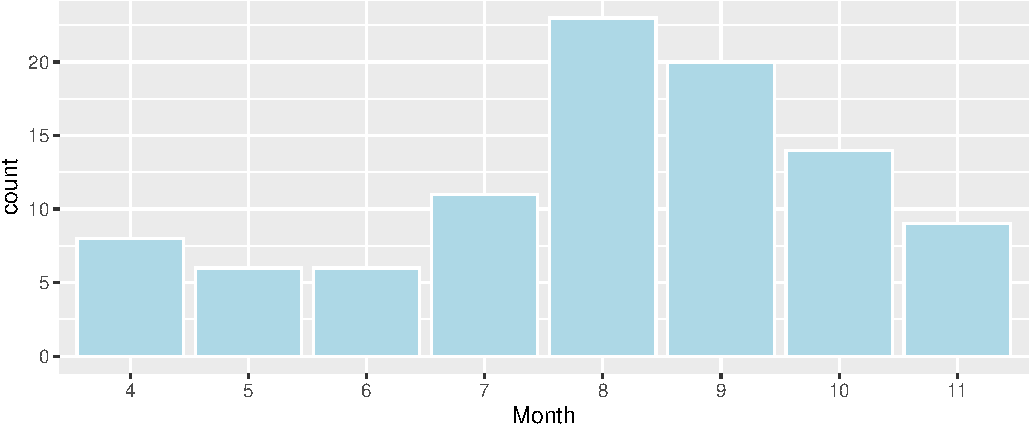
\includegraphics{_main_files/figure-latex/unnamed-chunk-86-1.pdf}

Notice that there are no measurements between December and March, the
bears' hibernation season.

\subsection{Season Variable}\label{season-variable}

When a variable has many categories, it becomes harder to compare the
categories. Sometimes, it is helpful to create a new variable with fewer
variables by combining categories.

Let's combine the months of April and May into a category called
``Spring'', June, July, and August into ``Summer'', and ``September'',
``October'', and ``November'', into ``Fall''.

\begin{Shaded}
\begin{Highlighting}[]
\NormalTok{Bears_Subset <-}\StringTok{ }\NormalTok{Bears_Subset }\OperatorTok\StringTok{ }\KeywordTok{mutate}\NormalTok{(}\DataTypeTok{Season =} \KeywordTok{ifelse}\NormalTok{(Month }\OperatorTok\StringTok{ }\DecValTok{4}\OperatorTok{:}\DecValTok{5}\NormalTok{, }\StringTok{"Spring"}\NormalTok{,}
\KeywordTok{ifelse}\NormalTok{(Month }\OperatorTok\StringTok{ }\DecValTok{6}\OperatorTok{:}\DecValTok{8}\NormalTok{, }\StringTok{"Summer"}\NormalTok{, }\StringTok{"Fall"}\NormalTok{)))}
\NormalTok{Bears_Subset}\OperatorTok{$}\NormalTok{Season <-}\StringTok{ }\KeywordTok{as.factor}\NormalTok{(Bears_Subset}\OperatorTok{$}\NormalTok{Season)}
\end{Highlighting}
\end{Shaded}

\subsection{Visualizing Season
Variable}\label{visualizing-season-variable}

\begin{Shaded}
\begin{Highlighting}[]
\KeywordTok{ggplot}\NormalTok{(}\DataTypeTok{data=}\NormalTok{Bears_Subset, }\KeywordTok{aes}\NormalTok{(}\DataTypeTok{x=}\NormalTok{Season)) }\OperatorTok{+}\StringTok{ }\KeywordTok{geom_bar}\NormalTok{(}\DataTypeTok{color=}\StringTok{"white"}\NormalTok{, }\DataTypeTok{fill=}\StringTok{"lightblue"}\NormalTok{)}
\end{Highlighting}
\end{Shaded}

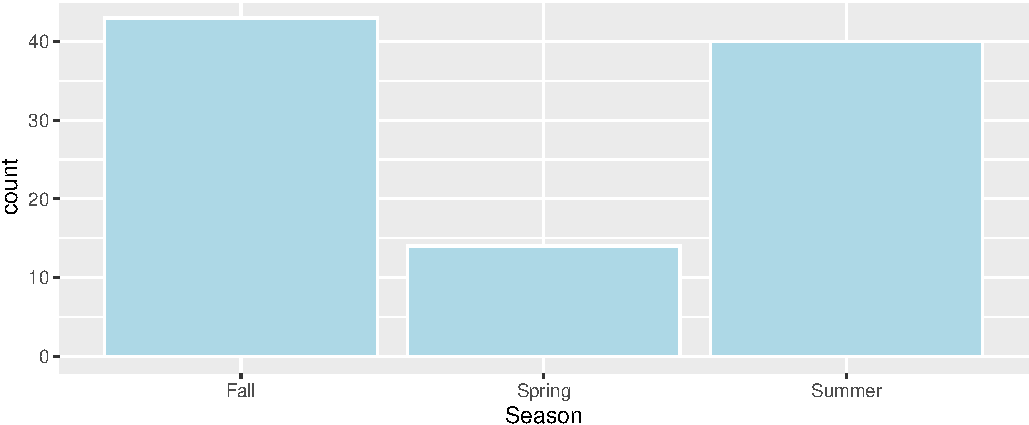
\includegraphics{_main_files/figure-latex/unnamed-chunk-88-1.pdf}

\subsection{Bears Data Summary}\label{bears-data-summary}

\begin{Shaded}
\begin{Highlighting}[]
\KeywordTok{summary}\NormalTok{(Bears_Subset)}
\end{Highlighting}
\end{Shaded}

\begin{verbatim}
##        ID             Age             Month    Sex        Head.L     
##  Min.   : 39.0   Min.   :  8.00   8      :23   1:62   Min.   : 9.00  
##  1st Qu.:525.0   1st Qu.: 17.00   9      :20   2:35   1st Qu.:12.00  
##  Median :579.0   Median : 34.00   10     :14          Median :13.00  
##  Mean   :537.6   Mean   : 42.64   7      :11          Mean   :13.29  
##  3rd Qu.:640.0   3rd Qu.: 57.25   11     : 9          3rd Qu.:14.50  
##  Max.   :911.0   Max.   :177.00   4      : 8          Max.   :18.50  
##                  NA's   :41       (Other):12                         
##      Head.W           Neck.G          Length         Chest.G     
##  Min.   : 4.000   Min.   :10.00   Min.   :36.00   Min.   :19.00  
##  1st Qu.: 5.000   1st Qu.:17.50   1st Qu.:54.50   1st Qu.:30.00  
##  Median : 6.000   Median :20.00   Median :61.00   Median :34.00  
##  Mean   : 6.364   Mean   :21.03   Mean   :60.41   Mean   :35.93  
##  3rd Qu.: 7.000   3rd Qu.:24.00   3rd Qu.:67.00   3rd Qu.:42.00  
##  Max.   :10.000   Max.   :32.00   Max.   :83.00   Max.   :55.00  
##                                                                  
##      Weight          Obs.No       Name       Season  
##  Min.   : 26.0   Min.   :1   Ian    : 2   Fall  :43  
##  1st Qu.:114.0   1st Qu.:1   Abe    : 1   Spring:14  
##  Median :154.0   Median :1   Addy   : 1   Summer:40  
##  Mean   :187.2   Mean   :1   Albert : 1              
##  3rd Qu.:236.0   3rd Qu.:1   Allen  : 1              
##  Max.   :514.0   Max.   :1   (Other):89              
##                              NA's   : 2
\end{verbatim}

\subsection{Histogram of Bear Weights}\label{histogram-of-bear-weights}

\begin{Shaded}
\begin{Highlighting}[]
\KeywordTok{ggplot}\NormalTok{(}\DataTypeTok{data=}\NormalTok{Bears_Subset, }\KeywordTok{aes}\NormalTok{(}\DataTypeTok{x=}\NormalTok{Weight)) }\OperatorTok{+}\StringTok{ }
\StringTok{  }\KeywordTok{geom_histogram}\NormalTok{(}\DataTypeTok{color=}\StringTok{"white"}\NormalTok{, }\DataTypeTok{fill=}\StringTok{"lightblue"}\NormalTok{) }\OperatorTok{+}\StringTok{ }
\StringTok{  }\KeywordTok{xlab}\NormalTok{(}\StringTok{"Weight"}\NormalTok{) }\OperatorTok{+}\StringTok{ }\KeywordTok{ylab}\NormalTok{(}\StringTok{"Frequency"}\NormalTok{) }\OperatorTok{+}\StringTok{ }\KeywordTok{ggtitle}\NormalTok{(}\StringTok{"Weights of Bears"}\NormalTok{)}
\end{Highlighting}
\end{Shaded}

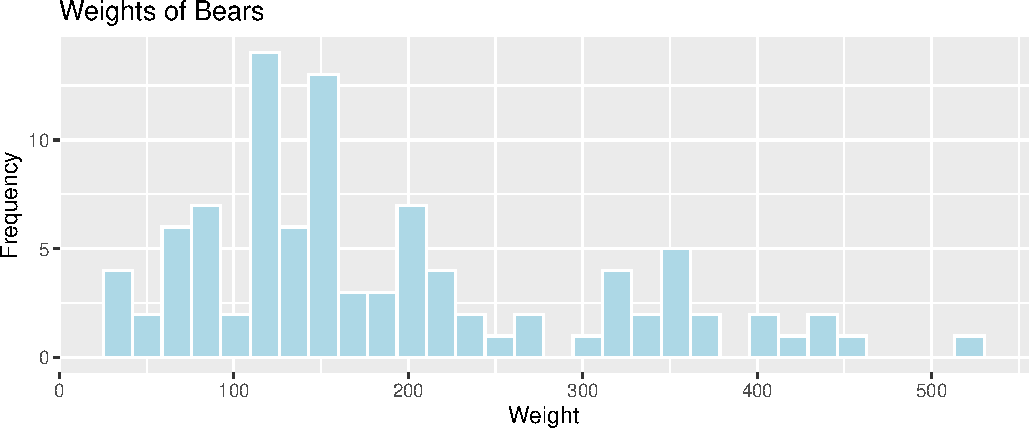
\includegraphics{_main_files/figure-latex/unnamed-chunk-90-1.pdf}

We see that bears most commonly weigh between 100 and 200 lbs, and the
distribution of weights is right-skewed.

\subsection{Weight by Season}\label{weight-by-season}

\begin{Shaded}
\begin{Highlighting}[]
\KeywordTok{ggplot}\NormalTok{(}\DataTypeTok{data=}\NormalTok{Bears_Subset, }\KeywordTok{aes}\NormalTok{(}\DataTypeTok{x=}\NormalTok{Season, }\DataTypeTok{y=}\NormalTok{Weight)) }\OperatorTok{+}\StringTok{ }\KeywordTok{geom_boxplot}\NormalTok{() }\OperatorTok{+}\StringTok{ }\KeywordTok{geom_jitter}\NormalTok{() }
\end{Highlighting}
\end{Shaded}

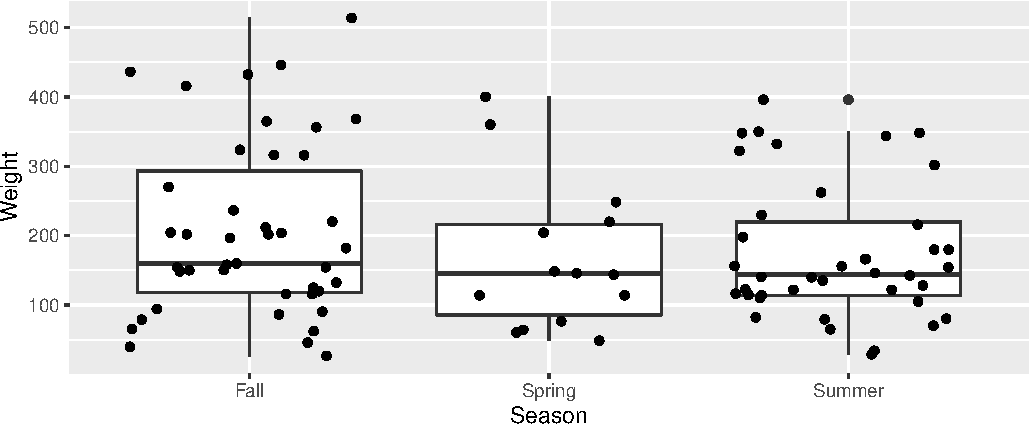
\includegraphics{_main_files/figure-latex/unnamed-chunk-91-1.pdf}

\subsection{Boxplot of Weight and Sex}\label{boxplot-of-weight-and-sex}

\begin{Shaded}
\begin{Highlighting}[]
\KeywordTok{ggplot}\NormalTok{(}\DataTypeTok{data=}\NormalTok{Bears_Subset, }\KeywordTok{aes}\NormalTok{(}\DataTypeTok{y=}\NormalTok{Weight, }\DataTypeTok{x=}\NormalTok{Sex)) }\OperatorTok{+}\StringTok{ }
\StringTok{  }\KeywordTok{geom_boxplot}\NormalTok{() }\OperatorTok{+}\StringTok{ }
\StringTok{  }\KeywordTok{xlab}\NormalTok{(}\StringTok{"Sex(1=M, 2=F)"}\NormalTok{) }\OperatorTok{+}\StringTok{ }\KeywordTok{ylab}\NormalTok{(}\StringTok{"Weight"}\NormalTok{) }\OperatorTok{+}\StringTok{ }\KeywordTok{ggtitle}\NormalTok{(}\StringTok{"Weight by Sex"}\NormalTok{) }\OperatorTok{+}\StringTok{ }\KeywordTok{coord_flip}\NormalTok{()}
\end{Highlighting}
\end{Shaded}

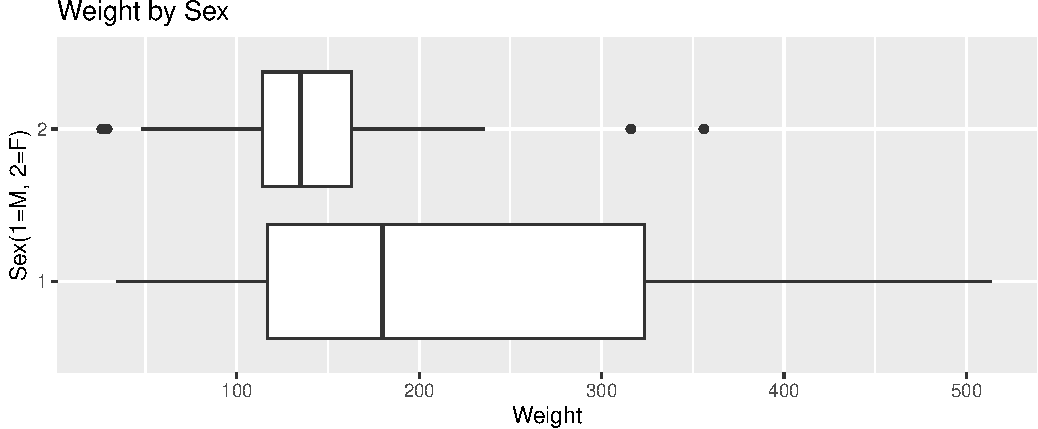
\includegraphics{_main_files/figure-latex/unnamed-chunk-92-1.pdf}

We see that male bears (Category 1) weigh more than female bears on
average, and that there is more variability in the weights of male bears
than female bears.

\subsection{Bears: Season and Sex Model without
Interaction}\label{bears-season-and-sex-model-without-interaction}

\(\widehat{\text{Weight}} = b_0+b_1\times\text{I}_{\text{Spring}}+b_2\times\text{I}_{\text{Summer}} + b_3\times\text{I}_{\text{Female}}\)

\begin{longtable}[]{@{}lll@{}}
\toprule
Season & Male & Female\tabularnewline
\midrule
\endhead
Fall & \(b_0\) & \(b_0 + b_3\)\tabularnewline
Spring & \(b_0 + b_1\) & \(b_0 + b_1+ b_3\)\tabularnewline
Summer & \(b_0 + b_2\) & \(b_0 + b_2+ b_3\)\tabularnewline
\bottomrule
\end{longtable}

\textbf{Model Assumptions}:

\begin{itemize}
\tightlist
\item
  Allows weights to differ by sex and season.\\
\item
  Assumes difference between sexes is the same in each season and
  difference between seasons is the same for each sex.
\end{itemize}

\subsection{Bears Season and Sex Model
Output}\label{bears-season-and-sex-model-output}

Let's model weights of male and female bears individually by season.

\begin{Shaded}
\begin{Highlighting}[]
\NormalTok{Bears_M_Season_Sex <-}\StringTok{ }\KeywordTok{lm}\NormalTok{(}\DataTypeTok{data=}\NormalTok{Bears_Subset, Weight}\OperatorTok{~}\NormalTok{Season }\OperatorTok{+}\StringTok{ }\NormalTok{Sex)}
\KeywordTok{summary}\NormalTok{(Bears_M_Season_Sex)}
\end{Highlighting}
\end{Shaded}

\begin{verbatim}
## 
## Call:
## lm(formula = Weight ~ Season + Sex, data = Bears_Subset)
## 
## Residuals:
##     Min      1Q  Median      3Q     Max 
## -186.73  -76.56  -17.32   63.44  287.27 
## 
## Coefficients:
##              Estimate Std. Error t value             Pr(>|t|)    
## (Intercept)    226.73      18.14  12.500 < 0.0000000000000002 ***
## SeasonSpring   -25.54      33.56  -0.761              0.44856    
## SeasonSummer   -28.17      23.79  -1.184              0.23939    
## Sex2           -67.24      23.06  -2.916              0.00445 ** 
## ---
## Signif. codes:  0 '***' 0.001 '**' 0.01 '*' 0.05 '.' 0.1 ' ' 1
## 
## Residual standard error: 108.3 on 93 degrees of freedom
## Multiple R-squared:  0.1024, Adjusted R-squared:  0.07343 
## F-statistic: 3.536 on 3 and 93 DF,  p-value: 0.01774
\end{verbatim}

\subsection{Predictions using Season and
Sex}\label{predictions-using-season-and-sex}

\(\widehat{\text{Weight}} = 226.73-25.54 \times\text{I}_{\text{Spring}}-28.17\times\text{I}_{\text{Summer}} -67.24\times\text{I}_{\text{Female}}\)

\begin{longtable}[]{@{}lll@{}}
\toprule
\begin{minipage}[b]{0.09\columnwidth}\raggedright\strut
\strut
\end{minipage} & \begin{minipage}[b]{0.14\columnwidth}\raggedright\strut
Male\strut
\end{minipage} & \begin{minipage}[b]{0.14\columnwidth}\raggedright\strut
Female\strut
\end{minipage}\tabularnewline
\midrule
\endhead
\begin{minipage}[t]{0.09\columnwidth}\raggedright\strut
Fall\strut
\end{minipage} & \begin{minipage}[t]{0.14\columnwidth}\raggedright\strut
226.73 - 25.54(0) - 28.17(0) -67.24(0)=226.73\strut
\end{minipage} & \begin{minipage}[t]{0.14\columnwidth}\raggedright\strut
226.73 - 25.54(0) - 28.17(0) -67.24(1)=159.59\strut
\end{minipage}\tabularnewline
\begin{minipage}[t]{0.09\columnwidth}\raggedright\strut
Spring\strut
\end{minipage} & \begin{minipage}[t]{0.14\columnwidth}\raggedright\strut
226.73 - 25.54(1) - 28.17(0) -67.24(0)=201.19\strut
\end{minipage} & \begin{minipage}[t]{0.14\columnwidth}\raggedright\strut
226.73 - 25.54(1) - 28.17(0) -67.24(1)=133.95\strut
\end{minipage}\tabularnewline
\begin{minipage}[t]{0.09\columnwidth}\raggedright\strut
Summer\strut
\end{minipage} & \begin{minipage}[t]{0.14\columnwidth}\raggedright\strut
226.73 - 25.54(0) - 28.17(1) -67.24(0)=198.55\strut
\end{minipage} & \begin{minipage}[t]{0.14\columnwidth}\raggedright\strut
226.73 - 25.54(0) - 28.17(1) -67.24(1)=131.32\strut
\end{minipage}\tabularnewline
\bottomrule
\end{longtable}

\subsection{Weight using Season and Sex Model
Interpretations}\label{weight-using-season-and-sex-model-interpretations}

\(\widehat{\text{Weight}} = 226.73-25.54 \times\text{I}_{\text{Spring}}-28.17\times\text{I}_{\text{Summer}} -67.24\times\text{I}_{\text{Female}}\)

Note that fall and male are treated as the ``baseline'' levels in this
model.

\begin{itemize}
\item
  On average, male bears are expected to weigh 226.73 lbs in the fall.
\item
  On average, bears of the same sex are expected to weigh 25.54 lbs less
  in the spring than in the fall.
\item
  On average, bears of the same sex are expected to weigh 28.17 lbs less
  in the summer than in the fall.
\item
  On average, female bears are expected to weigh 67.24 lbs than male
  bears, in the same season.
\end{itemize}

The model with season and sex explains about 10\% of the variation in
bear weights.

\subsection{Season and Sex with
Interaction}\label{season-and-sex-with-interaction}

\[\widehat{\text{Weight}} = b_0 + b_1 \times\text{I}_{\text{Spring}} + b_2\times\text{I}_{\text{Summer}} +b_3\times\text{I}_{\text{Female}}\\ +b_4\times\text{I}_{\text{Spring}}\text{I}_{\text{Female}} +b_5\times\text{I}_{\text{Summer}}\text{I}_{\text{Female}}\]

\begin{longtable}[]{@{}lll@{}}
\toprule
& Male & Female\tabularnewline
\midrule
\endhead
Fall & \(b_0\) & \(b_0+b_3\)\tabularnewline
Spring & \(b_0+b_1\) & \(b_0+b_1 +b_3+b_4\)\tabularnewline
Summer & \(b_0+b_2\) & \(b_0+b_2+b_3+b_5\)\tabularnewline
\bottomrule
\end{longtable}

\textbf{Model Assumptions}:

\begin{itemize}
\tightlist
\item
  Allows for differences between seasons and sexes.\\
\item
  Allows for differences between sexes to vary between seasons and
  difference between seasons to vary between sexes.
\end{itemize}

\(b_4\) and \(b_5\) are called \textbf{interaction effects}.

\subsection{Bears Season and Sex Interaction
Model}\label{bears-season-and-sex-interaction-model}

To fit an interaction model in R, use \texttt{*} instead of \texttt{+}

\begin{Shaded}
\begin{Highlighting}[]
\NormalTok{Bears_M_Season_Sex_Int <-}\StringTok{ }\KeywordTok{lm}\NormalTok{(}\DataTypeTok{data=}\NormalTok{Bears_Subset, Weight}\OperatorTok{~}\NormalTok{Season }\OperatorTok{*}\StringTok{ }\NormalTok{Sex)}
\KeywordTok{summary}\NormalTok{(Bears_M_Season_Sex_Int)}
\end{Highlighting}
\end{Shaded}

\begin{verbatim}
## 
## Call:
## lm(formula = Weight ~ Season * Sex, data = Bears_Subset)
## 
## Residuals:
##     Min      1Q  Median      3Q     Max 
## -181.14  -73.14  -13.07   58.81  292.86 
## 
## Coefficients:
##                   Estimate Std. Error t value            Pr(>|t|)    
## (Intercept)         221.14      20.28  10.905 <0.0000000000000002 ***
## SeasonSpring        -14.00      45.99  -0.304               0.762    
## SeasonSummer        -17.95      29.49  -0.608               0.544    
## Sex2                -50.07      35.54  -1.409               0.162    
## SeasonSpring:Sex2   -29.08      68.34  -0.425               0.672    
## SeasonSummer:Sex2   -30.41      50.73  -0.599               0.550    
## ---
## Signif. codes:  0 '***' 0.001 '**' 0.01 '*' 0.05 '.' 0.1 ' ' 1
## 
## Residual standard error: 109.2 on 91 degrees of freedom
## Multiple R-squared:  0.1064, Adjusted R-squared:  0.0573 
## F-statistic: 2.167 on 5 and 91 DF,  p-value: 0.06458
\end{verbatim}

\subsection{Predictions for Season and Sex Interaction
Model}\label{predictions-for-season-and-sex-interaction-model}

\[\widehat{\text{Weight}} = b_0 + b_1 \times\text{I}_{\text{Spring}} + b_2\times\text{I}_{\text{Summer}} +b_3\times\text{I}_{\text{Female}}\\ +b_4\times\text{I}_{\text{Spring}}\text{I}_{\text{Female}} +b_5\times\text{I}_{\text{Summer}}\text{I}_{\text{Female}}\]

\[
\begin{aligned}
\widehat{\text{Weight}} &= 221.14 -14.00 \times\text{I}_{\text{Spring}} -17.95\times\text{I}_{\text{Summer}} -50.07\times\text{I}_{\text{Female}} \\
&-29.08\times\text{I}_{\text{Spring}}\text{I}_{\text{Female}} -30.41\times\text{I}_{\text{Summer}}\text{I}_{\text{Female}}
\end{aligned}
\]

\begin{longtable}[]{@{}lll@{}}
\toprule
\begin{minipage}[b]{0.09\columnwidth}\raggedright\strut
\strut
\end{minipage} & \begin{minipage}[b]{0.14\columnwidth}\raggedright\strut
Male\strut
\end{minipage} & \begin{minipage}[b]{0.14\columnwidth}\raggedright\strut
Female\strut
\end{minipage}\tabularnewline
\midrule
\endhead
\begin{minipage}[t]{0.09\columnwidth}\raggedright\strut
Fall\strut
\end{minipage} & \begin{minipage}[t]{0.14\columnwidth}\raggedright\strut
221.14 -14.00(0) -17.95(0) -50.07(0) -29.08(0)(0)
-30.41(0)(0)=221.14\strut
\end{minipage} & \begin{minipage}[t]{0.14\columnwidth}\raggedright\strut
221.14 -14.00(0) -17.95(0) -50.07(1) -29.08(0)(1) -30.41(0)(1)
=171.07\strut
\end{minipage}\tabularnewline
\begin{minipage}[t]{0.09\columnwidth}\raggedright\strut
Spring\strut
\end{minipage} & \begin{minipage}[t]{0.14\columnwidth}\raggedright\strut
221.14 -14.00(1) -17.95(0) -50.07(0) -29.08(1)(0) -30.41(0)(0)
=207.14\strut
\end{minipage} & \begin{minipage}[t]{0.14\columnwidth}\raggedright\strut
211.375 + 8.01221.14 -14.00(1) -17.95(0) -50.07(1) -29.08(1)(1)
-30.41(0)(1)=128.00\strut
\end{minipage}\tabularnewline
\begin{minipage}[t]{0.09\columnwidth}\raggedright\strut
Summer\strut
\end{minipage} & \begin{minipage}[t]{0.14\columnwidth}\raggedright\strut
221.14 -14.00(0) -17.95(1) -50.07(0) -29.08(0)(0) -30.41(1)(0)
=203.19\strut
\end{minipage} & \begin{minipage}[t]{0.14\columnwidth}\raggedright\strut
221.14 -14.00(0) -17.95(1) -50.07(1) -29.08(0)(1) -30.41(1)(1)
=122.71\strut
\end{minipage}\tabularnewline
\bottomrule
\end{longtable}

\subsection{Season and Sex Interaction Model
Interpretations}\label{season-and-sex-interaction-model-interpretations}

\[\widehat{\text{Weight}} = b_0 + b_1 \times\text{I}_{\text{Spring}} + b_2\times\text{I}_{\text{Summer}} +b_3\times\text{I}_{\text{Female}}\\ +b_4\times\text{I}_{\text{Spring}}\text{I}_{\text{Female}} +b_5\times\text{I}_{\text{Summer}}\text{I}_{\text{Female}}\]

\begin{longtable}[]{@{}lll@{}}
\toprule
& Male & Female\tabularnewline
\midrule
\endhead
Fall & \(b_0\) & \(b_0+b_3\)\tabularnewline
Spring & \(b_0+b_1\) & \(b_0+b_1 +b_3+b_4\)\tabularnewline
Summer & \(b_0+b_2\) & \(b_0+b_2+b_3+b_5\)\tabularnewline
\bottomrule
\end{longtable}

\begin{itemize}
\tightlist
\item
  \(b_0\) represents expected weight of male bear in fall\\
\item
  \(b_1\) represents difference between expected male bear weight in
  spring, compared to fall\\
\item
  \(b_2\) represents difference between expected male bear weight in
  summer, compared to fall\\
\item
  \(b_3\) represents difference between expected female bear weight,
  compared to male bear weight in fall\\
\item
  \(b_4\) represents difference in expected weights between the sexes in
  the spring, compared to the difference in the fall\\
\item
  \(b_5\) represents difference in expected weights between the sexes in
  the summer, compared to the difference in the fall
\end{itemize}

\subsection{Interpretations for Season and Sex Interaction
Model}\label{interpretations-for-season-and-sex-interaction-model}

\[
\begin{aligned}
\widehat{\text{Weight}} &= 221.14 -14.00 \times\text{I}_{\text{Spring}} -17.95\times\text{I}_{\text{Summer}} -50.07\times\text{I}_{\text{Female}} \\
&-29.08\times\text{I}_{\text{Spring}}\text{I}_{\text{Female}} -30.41\times\text{I}_{\text{Summer}}\text{I}_{\text{Female}}
\end{aligned}
\]

\begin{itemize}
\tightlist
\item
  On average, male bears are expected to weigh 221.14 lbs in the fall.\\
\item
  On average male bears are expected to weigh 14 lbs less in the spring
  than in the fall.\\
\item
  On average, male bears are expected to weigh 17.95 lbs less in the
  summer than in the fall.\\
\item
  On average, female bears are expected to weigh 50.07 lbs less than
  male bears in the fall.\\
\item
  On average, the female bears are expected to weigh 29.08 lbs. less
  relative to male bears in the spring, compared to the expected
  difference the fall. Thus, female bears are expected to weigh 50.07 +
  29.08 = 79.17 lbs less than male bears in the spring.\\
\item
  On average, female bears are expected to weigh 30.41 lbs less,
  relative to male bears in the summer, compared to the expected
  difference in the fall. Thus, female bears are expected to weigh
  \(50.07 + 30.41 = 80.48\) lbs less than male bears in the summer.
\end{itemize}

The interaction model explains about 10.6\% of the variation in bear
weights.

\subsection{Predicting New Observations in
R}\label{predicting-new-observations-in-r}

We can calculate predictions directly in R by putting the new data in a
data.frame and calling the \texttt{predict()} function.

\begin{Shaded}
\begin{Highlighting}[]
\NormalTok{Season <-}\StringTok{ }\KeywordTok{c}\NormalTok{(}\StringTok{"Fall"}\NormalTok{, }\StringTok{"Fall"}\NormalTok{, }\StringTok{"Spring"}\NormalTok{, }\StringTok{"Spring"}\NormalTok{, }\StringTok{"Summer"}\NormalTok{, }\StringTok{"Summer"}\NormalTok{)}
\NormalTok{Sex <-}\StringTok{ }\KeywordTok{factor}\NormalTok{(}\KeywordTok{c}\NormalTok{(}\DecValTok{1}\NormalTok{,}\DecValTok{2}\NormalTok{,}\DecValTok{1}\NormalTok{,}\DecValTok{2}\NormalTok{,}\DecValTok{1}\NormalTok{,}\DecValTok{2}\NormalTok{))}
\NormalTok{NewBears <-}\StringTok{ }\KeywordTok{data.frame}\NormalTok{(Season, Sex)}
\end{Highlighting}
\end{Shaded}

\begin{Shaded}
\begin{Highlighting}[]
\KeywordTok{predict}\NormalTok{(Bears_M_Season_Sex, }\DataTypeTok{newdata=}\NormalTok{NewBears)}
\end{Highlighting}
\end{Shaded}

\begin{verbatim}
##        1        2        3        4        5        6 
## 226.7290 159.4900 201.1909 133.9520 198.5586 131.3197
\end{verbatim}

\begin{Shaded}
\begin{Highlighting}[]
\KeywordTok{predict}\NormalTok{(Bears_M_Season_Sex_Int, }\DataTypeTok{newdata=}\NormalTok{NewBears)}
\end{Highlighting}
\end{Shaded}

\begin{verbatim}
##        1        2        3        4        5        6 
## 221.1379 171.0714 207.1429 128.0000 203.1923 122.7143
\end{verbatim}

\section{Interaction Models with Categorical and Quantitative
Variables}\label{interaction-models-with-categorical-and-quantitative-variables}

\subsection{Summary of Bears Dataset}\label{summary-of-bears-dataset}

\begin{Shaded}
\begin{Highlighting}[]
\KeywordTok{summary}\NormalTok{(Bears_Subset)}
\end{Highlighting}
\end{Shaded}

\begin{verbatim}
##        ID             Age             Month    Sex        Head.L     
##  Min.   : 39.0   Min.   :  8.00   8      :23   1:62   Min.   : 9.00  
##  1st Qu.:525.0   1st Qu.: 17.00   9      :20   2:35   1st Qu.:12.00  
##  Median :579.0   Median : 34.00   10     :14          Median :13.00  
##  Mean   :537.6   Mean   : 42.64   7      :11          Mean   :13.29  
##  3rd Qu.:640.0   3rd Qu.: 57.25   11     : 9          3rd Qu.:14.50  
##  Max.   :911.0   Max.   :177.00   4      : 8          Max.   :18.50  
##                  NA's   :41       (Other):12                         
##      Head.W           Neck.G          Length         Chest.G     
##  Min.   : 4.000   Min.   :10.00   Min.   :36.00   Min.   :19.00  
##  1st Qu.: 5.000   1st Qu.:17.50   1st Qu.:54.50   1st Qu.:30.00  
##  Median : 6.000   Median :20.00   Median :61.00   Median :34.00  
##  Mean   : 6.364   Mean   :21.03   Mean   :60.41   Mean   :35.93  
##  3rd Qu.: 7.000   3rd Qu.:24.00   3rd Qu.:67.00   3rd Qu.:42.00  
##  Max.   :10.000   Max.   :32.00   Max.   :83.00   Max.   :55.00  
##                                                                  
##      Weight          Obs.No       Name       Season  
##  Min.   : 26.0   Min.   :1   Ian    : 2   Fall  :43  
##  1st Qu.:114.0   1st Qu.:1   Abe    : 1   Spring:14  
##  Median :154.0   Median :1   Addy   : 1   Summer:40  
##  Mean   :187.2   Mean   :1   Albert : 1              
##  3rd Qu.:236.0   3rd Qu.:1   Allen  : 1              
##  Max.   :514.0   Max.   :1   (Other):89              
##                              NA's   : 2
\end{verbatim}

\subsection{Histogram of Bear Ages}\label{histogram-of-bear-ages}

\begin{Shaded}
\begin{Highlighting}[]
\KeywordTok{ggplot}\NormalTok{(}\DataTypeTok{data=}\NormalTok{Bears_Subset, }\KeywordTok{aes}\NormalTok{(}\DataTypeTok{x=}\NormalTok{Age)) }\OperatorTok{+}\StringTok{ }
\StringTok{  }\KeywordTok{geom_histogram}\NormalTok{(}\DataTypeTok{color=}\StringTok{"white"}\NormalTok{, }\DataTypeTok{fill=}\StringTok{"lightblue"}\NormalTok{) }\OperatorTok{+}\StringTok{ }
\StringTok{  }\KeywordTok{xlab}\NormalTok{(}\StringTok{"Age (in months)"}\NormalTok{) }\OperatorTok{+}\StringTok{ }\KeywordTok{ylab}\NormalTok{(}\StringTok{"Frequency"}\NormalTok{) }\OperatorTok{+}\StringTok{ }\KeywordTok{ggtitle}\NormalTok{(}\StringTok{"Ages of Bears (in months)"}\NormalTok{)}
\end{Highlighting}
\end{Shaded}

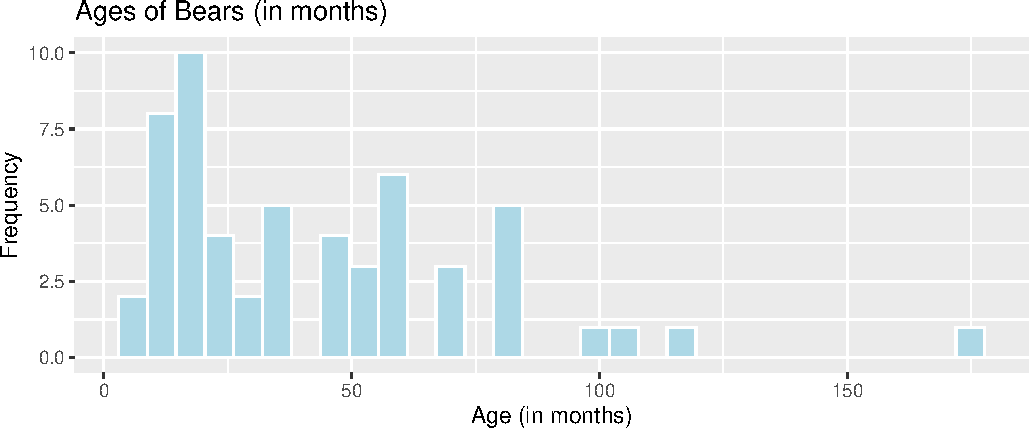
\includegraphics{_main_files/figure-latex/unnamed-chunk-99-1.pdf}

\subsection{Bears with Missing Ages}\label{bears-with-missing-ages}

Recall that 41 bears had missing ages. They will be ignored if we use
age in our model. To see how this might impact predicted weights, let's
look at how weights compare for bears with and without missing ages.

\begin{Shaded}
\begin{Highlighting}[]
\KeywordTok{ggplot}\NormalTok{(}\DataTypeTok{data=}\NormalTok{Bears_Subset, }\KeywordTok{aes}\NormalTok{(}\DataTypeTok{x=}\KeywordTok{is.na}\NormalTok{(Age), }\DataTypeTok{y=}\NormalTok{Weight)) }\OperatorTok{+}\StringTok{ }\KeywordTok{geom_boxplot}\NormalTok{() }\OperatorTok{+}\StringTok{ }\KeywordTok{coord_flip}\NormalTok{()}
\end{Highlighting}
\end{Shaded}

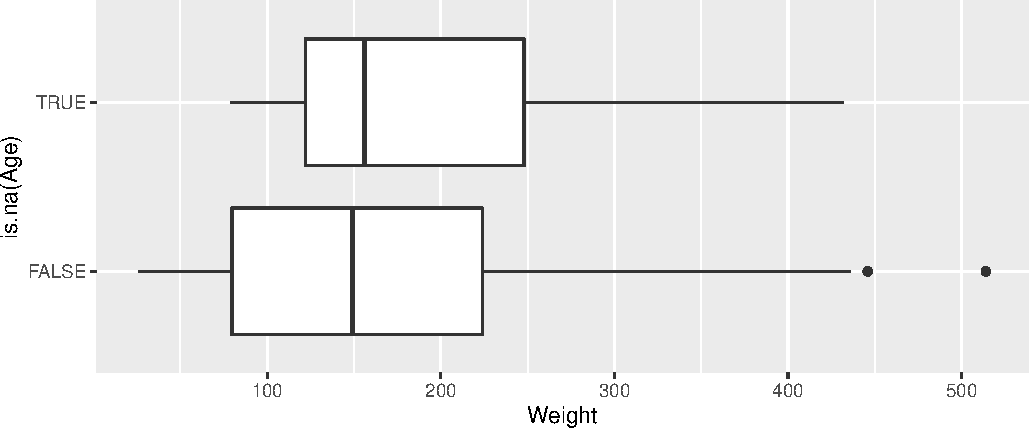
\includegraphics{_main_files/figure-latex/unnamed-chunk-100-1.pdf}

Bears with missing ages do not seem to be systematically different than
those whose ages are recorded, with respect to weight, so the missing
ages should not cause too much concern with out model results.

\subsection{Boxplot of Weight and
Sex}\label{boxplot-of-weight-and-sex-1}

\begin{Shaded}
\begin{Highlighting}[]
\KeywordTok{ggplot}\NormalTok{(}\DataTypeTok{data=}\NormalTok{Bears_Subset, }\KeywordTok{aes}\NormalTok{(}\DataTypeTok{y=}\NormalTok{Weight, }\DataTypeTok{x=}\NormalTok{Sex)) }\OperatorTok{+}\StringTok{ }
\StringTok{  }\KeywordTok{geom_boxplot}\NormalTok{() }\OperatorTok{+}\StringTok{ }
\StringTok{  }\KeywordTok{xlab}\NormalTok{(}\StringTok{"Sex(1=M, 2=F)"}\NormalTok{) }\OperatorTok{+}\StringTok{ }\KeywordTok{ylab}\NormalTok{(}\StringTok{"Weight in lbs"}\NormalTok{) }\OperatorTok{+}\StringTok{ }\KeywordTok{ggtitle}\NormalTok{(}\StringTok{"Weight by Sex"}\NormalTok{) }\OperatorTok{+}\StringTok{ }\KeywordTok{coord_flip}\NormalTok{()}
\end{Highlighting}
\end{Shaded}

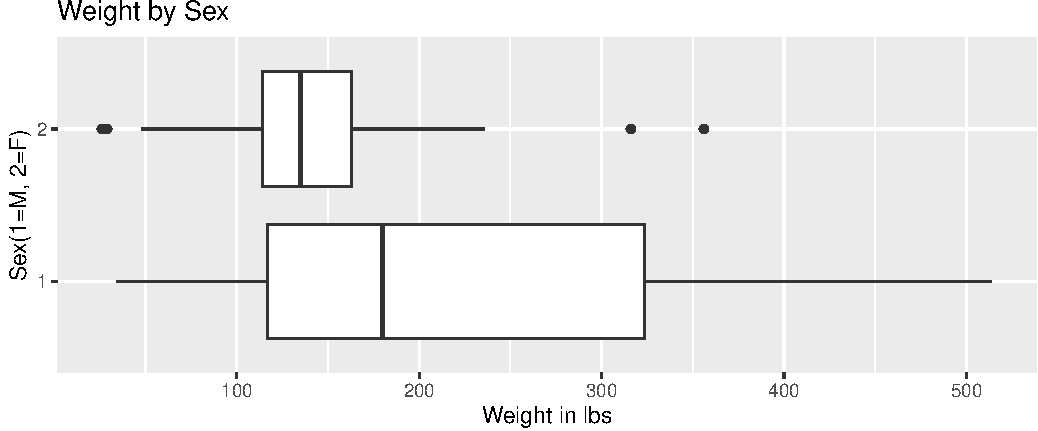
\includegraphics{_main_files/figure-latex/unnamed-chunk-101-1.pdf}

\subsection{Boxplot of Age and Sex}\label{boxplot-of-age-and-sex}

\begin{Shaded}
\begin{Highlighting}[]
\KeywordTok{ggplot}\NormalTok{(}\DataTypeTok{data=}\NormalTok{Bears_Subset, }\KeywordTok{aes}\NormalTok{(}\DataTypeTok{y=}\NormalTok{Age, }\DataTypeTok{x=}\NormalTok{Sex)) }\OperatorTok{+}\StringTok{ }
\StringTok{  }\KeywordTok{geom_boxplot}\NormalTok{() }\OperatorTok{+}\StringTok{ }
\StringTok{  }\KeywordTok{xlab}\NormalTok{(}\StringTok{"Sex(1=M, 2=F)"}\NormalTok{) }\OperatorTok{+}\StringTok{ }\KeywordTok{ylab}\NormalTok{(}\StringTok{"Age in Months"}\NormalTok{) }\OperatorTok{+}\StringTok{ }\KeywordTok{ggtitle}\NormalTok{(}\StringTok{"Age by Sex"}\NormalTok{) }\OperatorTok{+}\StringTok{ }\KeywordTok{coord_flip}\NormalTok{()}
\end{Highlighting}
\end{Shaded}

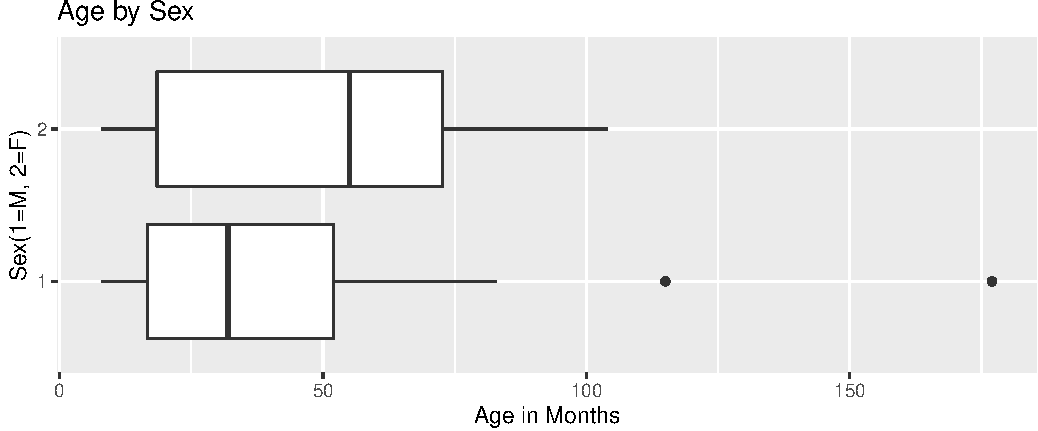
\includegraphics{_main_files/figure-latex/unnamed-chunk-102-1.pdf}

The median age for female bears is older than for male bears. There are
2 male bears that are much older than any others.

\subsection{Scatterplot of Age and
Weight}\label{scatterplot-of-age-and-weight}

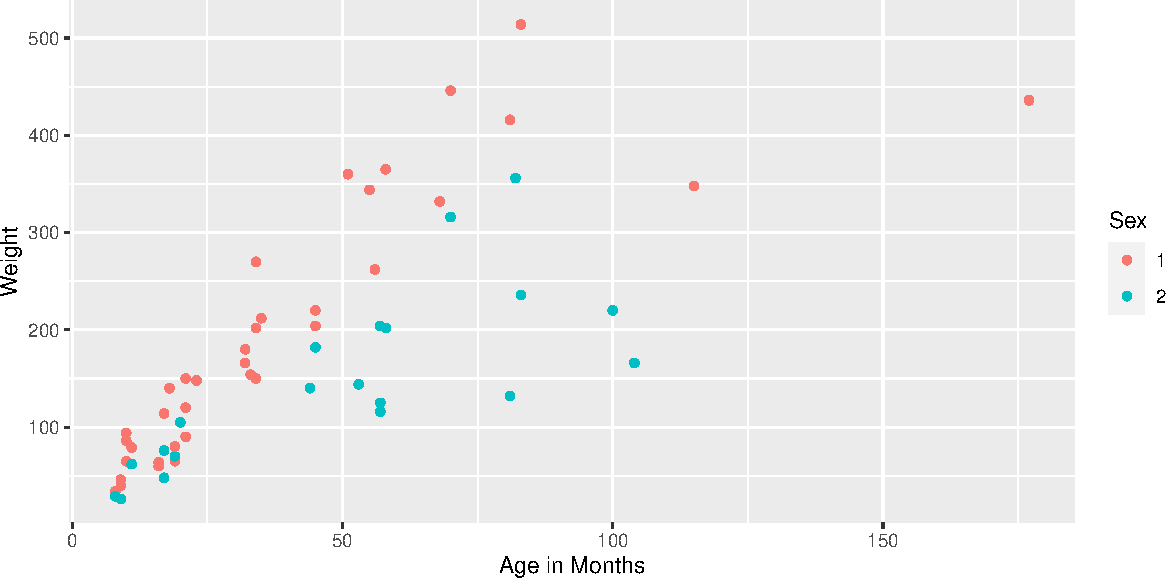
\includegraphics{_main_files/figure-latex/unnamed-chunk-103-1.pdf}

We see that there is a positive, roughly linear, relationship between
age and weight.

We should note that this linear trend is not likely to continue outside
the range of our observed ages.

\subsection{Bears: Age and Sex Model}\label{bears-age-and-sex-model}

\(\widehat{\text{Weight}}= b_0+ b_1 \times\text{Age}+ b_2\times\text{I}_{Female}\)

\begin{longtable}[]{@{}ll@{}}
\toprule
Sex & Pred. Weight\tabularnewline
\midrule
\endhead
M & \(b_0 + b_1 \times\text{Age}\)\tabularnewline
F & \((b_0 + b_2) + b_1 \times\text{Age}\)\tabularnewline
\bottomrule
\end{longtable}

\textbf{Model Assumptions:}

\begin{itemize}
\tightlist
\item
  Assumes weight increases linearly with age\\
\item
  Allows for differences in expected weight for male and female bears of
  same age\\
\item
  Assumes male and female bears gain weight at the same rate as they age
\end{itemize}

\subsection{Constant Slope Model for
Bears}\label{constant-slope-model-for-bears}

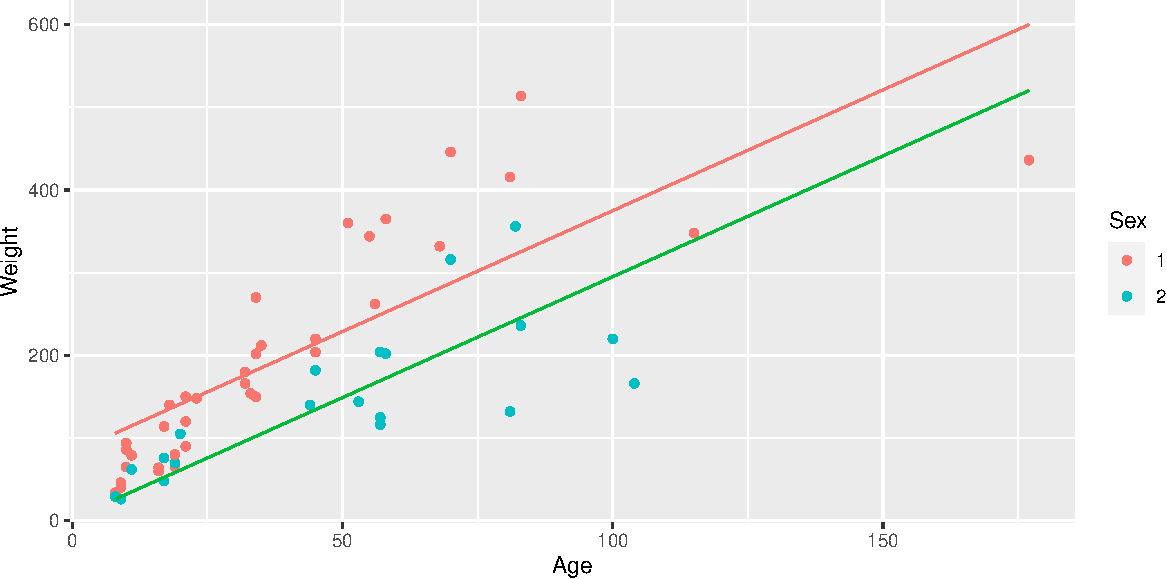
\includegraphics{_main_files/figure-latex/unnamed-chunk-105-1.pdf}

\subsection{Bears Age and Sex Model
Output}\label{bears-age-and-sex-model-output}

\begin{Shaded}
\begin{Highlighting}[]
\NormalTok{Bears_M_Age_Sex <-}\StringTok{ }\KeywordTok{lm}\NormalTok{(}\DataTypeTok{data=}\NormalTok{Bears_Subset, Weight }\OperatorTok{~}\StringTok{ }\NormalTok{Age }\OperatorTok{+}\StringTok{ }\NormalTok{Sex)}
\KeywordTok{summary}\NormalTok{(Bears_M_Age_Sex)}
\end{Highlighting}
\end{Shaded}

\begin{verbatim}
## 
## Call:
## lm(formula = Weight ~ Age + Sex, data = Bears_Subset)
## 
## Residuals:
##      Min       1Q   Median       3Q      Max 
## -164.194  -48.483   -3.723   27.766  188.684 
## 
## Coefficients:
##             Estimate Std. Error t value           Pr(>|t|)    
## (Intercept)  82.6049    16.4019   5.036 0.0000058437067215 ***
## Age           2.9242     0.2914  10.035 0.0000000000000744 ***
## Sex2        -79.8967    20.1416  -3.967            0.00022 ***
## ---
## Signif. codes:  0 '***' 0.001 '**' 0.01 '*' 0.05 '.' 0.1 ' ' 1
## 
## Residual standard error: 71.33 on 53 degrees of freedom
##   (41 observations deleted due to missingness)
## Multiple R-squared:  0.6679, Adjusted R-squared:  0.6554 
## F-statistic: 53.29 on 2 and 53 DF,  p-value: 0.0000000000002061
\end{verbatim}

\subsection{Predicted Bear Weights from Age and Sex
Model}\label{predicted-bear-weights-from-age-and-sex-model}

\(\widehat{\text{Weight}}= 82.60 + 2.92 \times\text{Age} - 79.90\times\text{I}_{Female}\)

Suppose Sally and Yogi are 25 month old bears, Sally is a female, Yogi a
male.

Sally's Predicted Weight:

\(\widehat{\text{Weight}}= 82.60 + 2.920 \times 25 -78.90\times 1 \approx 75.8 \text{ lbs.}\)

Yogi's Predicted Weight:

\(\widehat{\text{Weight}}= 82.60 + 2.920 \times 25 -78.90\times 0 \approx 155.7 \text{ lbs.}\)

\subsection{Age and Sex Model for Male and Female
Bears}\label{age-and-sex-model-for-male-and-female-bears}

The interaction model allows for different intercepts, but assumes that
the average monthly weight increase is the same for male and female
bears.

\(\widehat{\text{Weight}}= 82.60 + 2.92 \times\text{Age} - 79.90\times\text{I}_{Female}\)

Male Bears: \[
\widehat{\text{Weight}}= 82.60 + 2.92 \times\text{Age}
\]

Female Bears: \[
\widehat{\text{Weight}}= (82.60 -79.90) + (2.92)\times\text{Age} \\
= 2.7+2.92\times Age
\]

\subsection{\texorpdfstring{Bears Predictions with
\texttt{predict}}{Bears Predictions with predict}}\label{bears-predictions-with-predict}

\begin{Shaded}
\begin{Highlighting}[]
\NormalTok{Sex <-}\StringTok{ }\KeywordTok{factor}\NormalTok{(}\KeywordTok{c}\NormalTok{(}\DecValTok{1}\NormalTok{, }\DecValTok{2}\NormalTok{))}
\NormalTok{Age <-}\StringTok{ }\KeywordTok{c}\NormalTok{(}\DecValTok{25}\NormalTok{, }\DecValTok{25}\NormalTok{)}
\NormalTok{NewBears <-}\StringTok{ }\KeywordTok{data.frame}\NormalTok{(Age, Sex)}
\end{Highlighting}
\end{Shaded}

\begin{Shaded}
\begin{Highlighting}[]
\KeywordTok{predict}\NormalTok{(Bears_M_Age_Sex, }\DataTypeTok{newdata=}\NormalTok{NewBears)}
\end{Highlighting}
\end{Shaded}

\begin{verbatim}
##         1         2 
## 155.71061  75.81394
\end{verbatim}

\subsection{Age and Sex Model
Interpretations}\label{age-and-sex-model-interpretations}

\begin{itemize}
\item
  For bears of the same sex, weight is expected to increase by 2.92 lbs.
  each month.
\item
  On average, a female bear is expected to weigh 79.90 lbs less than a
  male bear of the same age.
\item
  The intercept \(b_0=82.60\) represents the expected weight of a male
  bear at birth. We should treat this interpretation with caution, since
  all bears in the dataset were at least 8 months old.
\end{itemize}

Approximately 67\% of the variation in bear weights is explained by the
model using age and sex as explanatory variables.

\subsection{Bears Age and Sex Model with
Interaction}\label{bears-age-and-sex-model-with-interaction}

\(\widehat{\text{Weight}}= b_0+ b_1 \times\text{Age}+ b_2\times\text{I}_{Female} + b_3\times\text{Age}\times\text{I}_{Female}\)

\begin{longtable}[]{@{}ll@{}}
\toprule
Sex & Pred. Weight\tabularnewline
\midrule
\endhead
M & \(b_0 + b_1 \times\text{Age}\)\tabularnewline
F & \((b_0 + b_2) + (b_1 + b_3) \times\text{Age}\)\tabularnewline
\bottomrule
\end{longtable}

\textbf{Model Assumptions:}

\begin{itemize}
\tightlist
\item
  Assumes weight increases linearly with age\\
\item
  Allows for differences in expected weight for male and female bears of
  same age\\
\item
  Allows male and female bears to gain weight at different rates as they
  age
\end{itemize}

\subsection{Bears Age and Sex Interaction
Model}\label{bears-age-and-sex-interaction-model}

\begin{Shaded}
\begin{Highlighting}[]
\KeywordTok{ggplot}\NormalTok{(}\DataTypeTok{data=}\NormalTok{Bears_Subset, }\KeywordTok{aes}\NormalTok{(}\DataTypeTok{x=}\NormalTok{Age, }\DataTypeTok{y=}\NormalTok{Weight, }\DataTypeTok{color=}\NormalTok{Sex)) }\OperatorTok{+}\StringTok{ }
\StringTok{  }\KeywordTok{geom_point}\NormalTok{() }\OperatorTok{+}\StringTok{ }\KeywordTok{stat_smooth}\NormalTok{(}\DataTypeTok{method=}\StringTok{"lm"}\NormalTok{, }\DataTypeTok{se=}\OtherTok{FALSE}\NormalTok{)}
\end{Highlighting}
\end{Shaded}

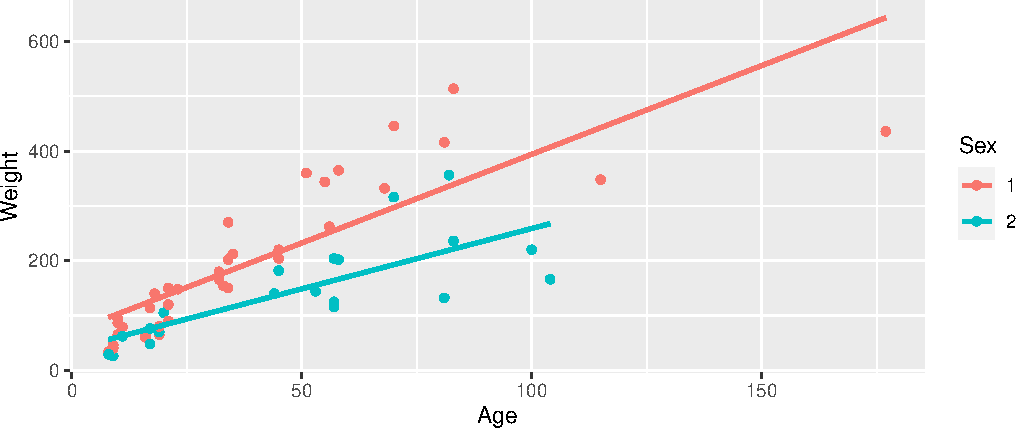
\includegraphics{_main_files/figure-latex/unnamed-chunk-109-1.pdf}

\subsection{Summary for Age-Sex Interaction
Model}\label{summary-for-age-sex-interaction-model}

\begin{Shaded}
\begin{Highlighting}[]
\NormalTok{Bears_M_Age_Sex_Int <-}\StringTok{ }\KeywordTok{lm}\NormalTok{(}\DataTypeTok{data=}\NormalTok{Bears_Subset, Weight}\OperatorTok{~}\StringTok{ }\NormalTok{Age}\OperatorTok{*}\NormalTok{Sex)}
\KeywordTok{summary}\NormalTok{(Bears_M_Age_Sex_Int)}
\end{Highlighting}
\end{Shaded}

\begin{verbatim}
## 
## Call:
## lm(formula = Weight ~ Age * Sex, data = Bears_Subset)
## 
## Residuals:
##      Min       1Q   Median       3Q      Max 
## -207.583  -38.854   -9.574   23.905  174.802 
## 
## Coefficients:
##             Estimate Std. Error t value          Pr(>|t|)    
## (Intercept)  70.4322    17.7260   3.973          0.000219 ***
## Age           3.2381     0.3435   9.428 0.000000000000765 ***
## Sex2        -31.9574    35.0314  -0.912          0.365848    
## Age:Sex2     -1.0350     0.6237  -1.659          0.103037    
## ---
## Signif. codes:  0 '***' 0.001 '**' 0.01 '*' 0.05 '.' 0.1 ' ' 1
## 
## Residual standard error: 70.18 on 52 degrees of freedom
##   (41 observations deleted due to missingness)
## Multiple R-squared:  0.6846, Adjusted R-squared:  0.6664 
## F-statistic: 37.62 on 3 and 52 DF,  p-value: 0.0000000000004552
\end{verbatim}

\subsection{Predictions from Interaction Model for
Bears}\label{predictions-from-interaction-model-for-bears}

\(\widehat{\text{Weight}}= 70.43 + 3.24 \times\text{Age}- 31.96\times\text{I}_{Female} -1.04\times\text{Age}\times\text{I}_{Female}\)

Suppose Sally and Yogi are 25 month old bears, Sally is a female, Yogi a
male.

Sally's Predicted Weight:

\(\widehat{\text{Weight}}= 70.43+ 3.24 \times 25- 31.96\times1 -1.04\times25\times1 \approx 93.55 \text{ lbs.}\)

Yogi's Predicted Weight:

\(\widehat{\text{Weight}}= 70.43+ 3.24 \times 25- 31.96\times0 -1.04\times25\times0 \approx 151.38 \text{ lbs.}\)

\subsection{Interaction Model for Male and Female
Bears}\label{interaction-model-for-male-and-female-bears}

The interaction model allow for different intercepts and slopes between
male and female bears.

\(\widehat{\text{Weight}}= 70.43 + 3.24 \times\text{Age}- 31.96\times\text{I}_{Female} -1.04\times\text{Age}\times\text{I}_{Female}\)

Male Bears: \[
\widehat{\text{Weight}}= 70.43 + 3.24 \times\text{Age}
\]

Female Bears: \[
\widehat{\text{Weight}}= (70.43 -31.96) + (3.24 -1.04)\times\text{Age} \\
= 38.46 + 2.20\times Age
\]

\subsection{\texorpdfstring{Bears Interaction Model Predictions with
\texttt{predict}}{Bears Interaction Model Predictions with predict}}\label{bears-interaction-model-predictions-with-predict}

\begin{Shaded}
\begin{Highlighting}[]
\NormalTok{Sex <-}\StringTok{ }\KeywordTok{factor}\NormalTok{(}\KeywordTok{c}\NormalTok{(}\DecValTok{1}\NormalTok{, }\DecValTok{2}\NormalTok{))}
\NormalTok{Age <-}\StringTok{ }\KeywordTok{c}\NormalTok{(}\DecValTok{25}\NormalTok{, }\DecValTok{25}\NormalTok{)}
\NormalTok{NewBears <-}\StringTok{ }\KeywordTok{data.frame}\NormalTok{(Age, Sex)}
\end{Highlighting}
\end{Shaded}

\begin{Shaded}
\begin{Highlighting}[]
\KeywordTok{predict}\NormalTok{(Bears_M_Age_Sex_Int, }\DataTypeTok{newdata=}\NormalTok{NewBears)}
\end{Highlighting}
\end{Shaded}

\begin{verbatim}
##         1         2 
## 151.38566  93.55306
\end{verbatim}

\subsection{Interpretations for Age and Sex Model with
Interaction}\label{interpretations-for-age-and-sex-model-with-interaction}

\(\widehat{\text{Weight}}= b_0+ b_1 \times\text{Age}+ b_2\times\text{I}_{Female} + b_3\times\text{Age}\times\text{I}_{Female}\)

\begin{longtable}[]{@{}ll@{}}
\toprule
Sex & Pred. Weight\tabularnewline
\midrule
\endhead
M & \(b_0 + b_1 \times\text{Age}\)\tabularnewline
F & \((b_0 + b_2) + (b_1 + b_3) \times\text{Age}\)\tabularnewline
\bottomrule
\end{longtable}

Interpretations:\\
\(b_0\): expected weight of a male bear at birth
(caution:extrapolation)\\
\(b_1\): expected weight gain per month for male bears\\
\(b_2\): expected difference in weight between female and male bears at
birth (caution:extrapolation)\\
\(b_3\): expected difference in monthly weight gain for female bears,
compared to male bears

\subsection{Bears Weight Model
Considerations}\label{bears-weight-model-considerations}

\begin{itemize}
\item
  \(R^2\) increased from 0.67 to 0.68 when the interaction term is
  added. This is a relatively small increase, so we might question
  whether the interaction term is needed.
\item
  The constant slope model allows us to combine information across sexes
  to estimate the expected slope. The interaction model treats the two
  sexes completely separately, thus has less information to use for each
  estimate.
\item
  Which model is preferable is not clear. In addition to the data, we
  should consider other relevent information. Do experts who study bears
  believe it is reasonable to assume that male and female bears grow at
  the same rate per month?
\item
  While the models yield drastically different predictions for very
  young bears, the differences are not as big for bear 8 months or
  older. Regardless of model we use, we should be careful about making
  predictions for bears that are younger or older than those that we
  have data on.
\end{itemize}

\subsection{Bears Weight Model Considerations
(continued)}\label{bears-weight-model-considerations-continued}

Both of these models contain assumptions that are probably unrealistic

\begin{itemize}
\item
  Both models assume that bears of the same sex gain weight linearly
  with age.
\item
  A more realistic model might assume that bears gain weight more
  quickly when they are younger, and that the rate of growth slows once
  they reach adulthood.
\item
  Are there variables not included in the model that might be predictive
  of a bear's weight?
\end{itemize}

Of course there is no statistical model that perfectly describes
expected weight gain of bears. The question is whether we can find a
model that provides an approximation that is reasonable enough to draw
conclusions from.

As statistician George Box famously said,

\emph{``All models are wrong, but some are useful.''}

\section{Interaction Models with Quantitative
Variables}\label{interaction-models-with-quantitative-variables}

\subsection{2015 Cars Dataset}\label{cars-dataset}

We consider data from the Kelly Blue Book, pertaining to new cars,
released in 2015. We'll investigate the relationship between price,
length, and time it takes to accelerate from 0 to 60 mph.

\begin{Shaded}
\begin{Highlighting}[]
\KeywordTok{data}\NormalTok{(Cars2015)}
\KeywordTok{glimpse}\NormalTok{(Cars2015)}
\end{Highlighting}
\end{Shaded}

\begin{verbatim}
## Rows: 110
## Columns: 20
## $ Make      <fct> Chevrolet, Hyundai, Kia, Mitsubishi, Nissan, Dodge, Chevrole~
## $ Model     <fct> Spark, Accent, Rio, Mirage, Versa Note, Dart, Cruze LS, 500L~
## $ Type      <fct> Hatchback, Hatchback, Sedan, Hatchback, Hatchback, Sedan, Se~
## $ LowPrice  <dbl> 12.270, 14.745, 13.990, 12.995, 14.180, 16.495, 16.170, 19.3~
## $ HighPrice <dbl> 25.560, 17.495, 18.290, 15.395, 17.960, 23.795, 25.660, 24.6~
## $ Drive     <fct> FWD, FWD, FWD, FWD, FWD, FWD, FWD, FWD, FWD, FWD, FWD, AWD, ~
## $ CityMPG   <int> 30, 28, 28, 37, 31, 23, 24, 24, 28, 30, 27, 27, 25, 27, 30, ~
## $ HwyMPG    <int> 39, 37, 36, 44, 40, 35, 36, 33, 38, 35, 33, 36, 36, 37, 39, ~
## $ FuelCap   <dbl> 9.0, 11.4, 11.3, 9.2, 10.9, 14.2, 15.6, 13.1, 12.4, 11.1, 11~
## $ Length    <int> 145, 172, 172, 149, 164, 184, 181, 167, 179, 154, 156, 180, ~
## $ Width     <int> 63, 67, 68, 66, 67, 72, 71, 70, 72, 67, 68, 69, 70, 68, 69, ~
## $ Wheelbase <int> 94, 101, 101, 97, 102, 106, 106, 103, 104, 99, 98, 104, 104,~
## $ Height    <int> 61, 57, 57, 59, 61, 58, 58, 66, 58, 59, 58, 58, 57, 58, 59, ~
## $ UTurn     <int> 34, 37, 37, 32, 37, 38, 38, 37, 39, 34, 35, 38, 37, 36, 37, ~
## $ Weight    <int> 2345, 2550, 2575, 2085, 2470, 3260, 3140, 3330, 2990, 2385, ~
## $ Acc030    <dbl> 4.4, 3.7, 3.5, 4.4, 4.0, 3.4, 3.7, 3.9, 3.4, 3.9, 3.9, 3.7, ~
## $ Acc060    <dbl> 12.8, 10.3, 9.5, 12.1, 10.9, 9.3, 9.8, 9.5, 9.2, 10.8, 11.1,~
## $ QtrMile   <dbl> 19.4, 17.8, 17.3, 19.0, 18.2, 17.2, 17.6, 17.4, 17.1, 18.3, ~
## $ PageNum   <int> 123, 148, 163, 188, 196, 128, 119, 131, 136, 216, 179, 205, ~
## $ Size      <fct> Small, Small, Small, Small, Small, Small, Small, Small, Smal~
\end{verbatim}

\subsection{Car Price and Acceleration
Time}\label{car-price-and-acceleration-time}

\texttt{LowPrice} represents the price of a standard (non-luxury) model
of a car. \texttt{Acc060} represents time it takes to accelerate from 0
to 60 mph.

\begin{Shaded}
\begin{Highlighting}[]
\KeywordTok{data}\NormalTok{(Cars2015)}
\end{Highlighting}
\end{Shaded}

\begin{Shaded}
\begin{Highlighting}[]
\NormalTok{CarsA060 <-}\StringTok{ }\KeywordTok{ggplot}\NormalTok{(}\DataTypeTok{data=}\NormalTok{Cars2015, }\KeywordTok{aes}\NormalTok{(}\DataTypeTok{x=}\NormalTok{Acc060, }\DataTypeTok{y=}\NormalTok{LowPrice)) }\OperatorTok{+}\StringTok{ }\KeywordTok{geom_point}\NormalTok{() }
\NormalTok{CarsA060}
\end{Highlighting}
\end{Shaded}

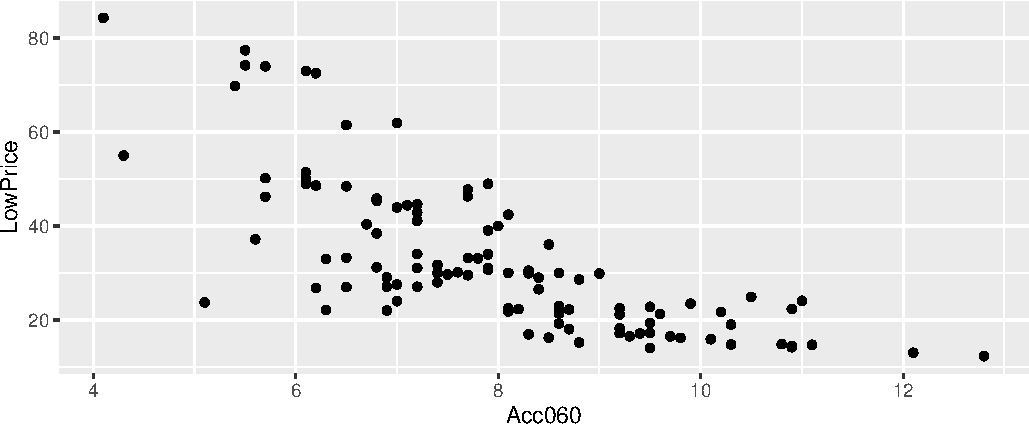
\includegraphics{_main_files/figure-latex/unnamed-chunk-115-1.pdf}

\subsection{Length and Sale Price}\label{length-and-sale-price}

\begin{Shaded}
\begin{Highlighting}[]
\KeywordTok{ggplot}\NormalTok{(}\DataTypeTok{data=}\NormalTok{Cars2015, }\KeywordTok{aes}\NormalTok{(}\DataTypeTok{x=}\NormalTok{Length, }\DataTypeTok{y=}\NormalTok{LowPrice)) }\OperatorTok{+}\StringTok{ }\KeywordTok{geom_point}\NormalTok{() }\OperatorTok{+}\StringTok{ }\KeywordTok{xlab}\NormalTok{(}\StringTok{"length in inches"}\NormalTok{)}
\end{Highlighting}
\end{Shaded}

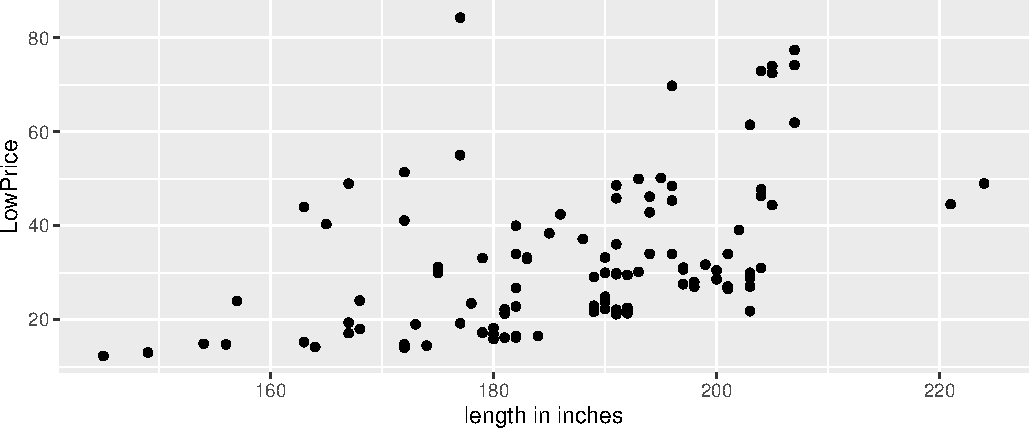
\includegraphics{_main_files/figure-latex/unnamed-chunk-116-1.pdf}

\subsection{Relationship between Acc060 and
Length}\label{relationship-between-acc060-and-length}

\begin{Shaded}
\begin{Highlighting}[]
\KeywordTok{ggplot}\NormalTok{(}\DataTypeTok{data=}\NormalTok{Cars2015, }\KeywordTok{aes}\NormalTok{(}\DataTypeTok{x=}\NormalTok{Length, }\DataTypeTok{y=}\NormalTok{Acc060)) }\OperatorTok{+}\StringTok{ }\KeywordTok{geom_point}\NormalTok{() }
\end{Highlighting}
\end{Shaded}

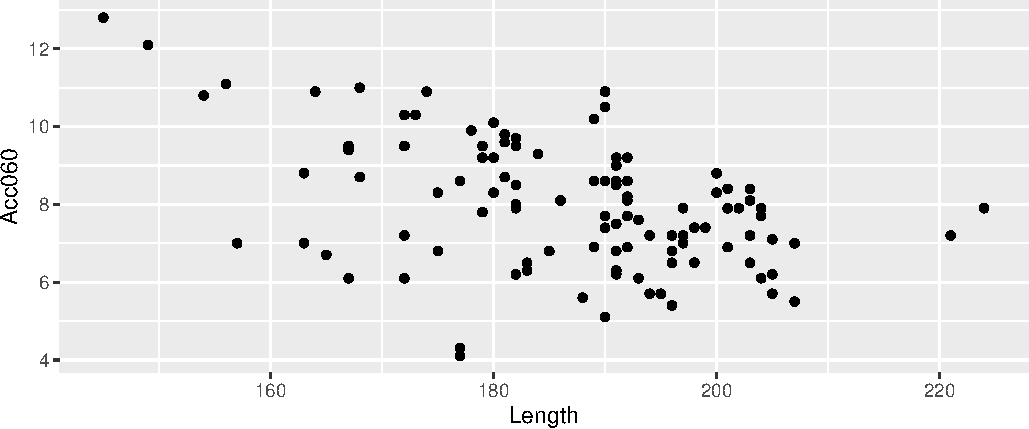
\includegraphics{_main_files/figure-latex/unnamed-chunk-117-1.pdf}

Lack of correlation among explanatory variables is a good thing. If
explanatory variables are highly correlated, then using them together is
unlikely to perform much better than using one or the other. In fact, it
can cause problems, as we'll see later.

\subsection{Modeling Price using
Acc060}\label{modeling-price-using-acc060}

\(\widehat{Price} = b_0 + b_1\times\text{Acc. Time}\)

\begin{itemize}
\tightlist
\item
  Model assumes expected price is a linear function of acceleration
  time.
\end{itemize}

Parameter Interpretations:

\(b_0\) represents intercept of regression line, i.e.~expected price of
a car that can accelerate from 0 to 60 mph in no time. This is not a
meaningful interpretation in context.

\(b_1\) represents slope of regression line, i.e.~expected change in
price for each additional second it takes to accelerate from 0 to 60
mph.

\subsection{Modeling for Car Price and
Acceleration}\label{modeling-for-car-price-and-acceleration}

\begin{Shaded}
\begin{Highlighting}[]
\NormalTok{Cars_M_A060 <-}\StringTok{ }\KeywordTok{lm}\NormalTok{(}\DataTypeTok{data=}\NormalTok{Cars2015, LowPrice}\OperatorTok{~}\NormalTok{Acc060)}
\KeywordTok{summary}\NormalTok{(Cars_M_A060)}
\end{Highlighting}
\end{Shaded}

\begin{verbatim}
## 
## Call:
## lm(formula = LowPrice ~ Acc060, data = Cars2015)
## 
## Residuals:
##     Min      1Q  Median      3Q     Max 
## -29.512  -6.544  -1.265   4.759  27.195 
## 
## Coefficients:
##             Estimate Std. Error t value            Pr(>|t|)    
## (Intercept)  89.9036     5.0523   17.79 <0.0000000000000002 ***
## Acc060       -7.1933     0.6234  -11.54 <0.0000000000000002 ***
## ---
## Signif. codes:  0 '***' 0.001 '**' 0.01 '*' 0.05 '.' 0.1 ' ' 1
## 
## Residual standard error: 10.71 on 108 degrees of freedom
## Multiple R-squared:  0.5521, Adjusted R-squared:  0.548 
## F-statistic: 133.1 on 1 and 108 DF,  p-value: < 0.00000000000000022
\end{verbatim}

\subsection{Price and A060 Regression
Line}\label{price-and-a060-regression-line}

\begin{Shaded}
\begin{Highlighting}[]
\NormalTok{CarsA060 }\OperatorTok{+}\StringTok{ }\KeywordTok{stat_smooth}\NormalTok{(}\DataTypeTok{method=}\StringTok{"lm"}\NormalTok{, }\DataTypeTok{se=}\OtherTok{FALSE}\NormalTok{)}
\end{Highlighting}
\end{Shaded}

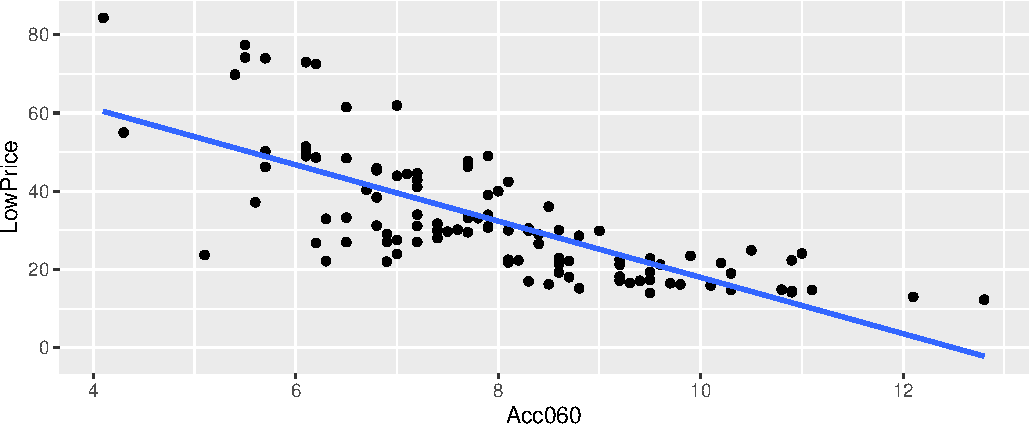
\includegraphics{_main_files/figure-latex/unnamed-chunk-119-1.pdf}

\subsection{Acc060 Model
Interpretations}\label{acc060-model-interpretations}

\(\widehat{Price} = b_0 + b_1\times\text{Acc. Time}\)

\(\widehat{Price} = 89.90 - 7.193\times\text{Acc. Time}\)

\begin{itemize}
\item
  Intercept \(b_0\) might be interpreted as the price of a car that can
  accelerate from 0 to 60 in no time, but this is not a meaningful
  interpretation since there are no such cars.
\item
  \(b_1=-7.1933\) tells us that on average, the price of a car is
  expected to decrease by 7.19 thousand dollars for each additional
  second it takes to accelerate from 0 to 60 mph.
\item
  \(R^2 = 0.5521\) tells us that 55\% of the variation in price is
  explained by the linear model using acceleration time as the
  explanatory variable.
\end{itemize}

\subsection{Modeling Price using Acc060 and
Length}\label{modeling-price-using-acc060-and-length}

\(\widehat{Price} = b_0 + b_1\times\text{Acc. Time} + b_2\times\text{Length}\)

\textbf{Model Assumptions:}

\begin{itemize}
\item
  Assumes expected price is a linear function of acceleration time and
  length.
\item
  Assumes that expected price increases at same rate with respect to
  acc. time, for cars of all lengths.
\item
  Assumes that expected price increases at same rate with respect to
  length, for cars of all acceleration times.
\end{itemize}

\subsection{Model Using Length and Acceleration
Time}\label{model-using-length-and-acceleration-time}

\begin{Shaded}
\begin{Highlighting}[]
\NormalTok{Cars_M_A060_L <-}\StringTok{ }\KeywordTok{lm}\NormalTok{(}\DataTypeTok{data=}\NormalTok{Cars2015, LowPrice }\OperatorTok{~}\StringTok{ }\NormalTok{Acc060 }\OperatorTok{+}\StringTok{ }\NormalTok{Length)}
\KeywordTok{summary}\NormalTok{(Cars_M_A060_L)}
\end{Highlighting}
\end{Shaded}

\begin{verbatim}
## 
## Call:
## lm(formula = LowPrice ~ Acc060 + Length, data = Cars2015)
## 
## Residuals:
##     Min      1Q  Median      3Q     Max 
## -27.969  -6.625  -1.418   4.934  28.394 
## 
## Coefficients:
##             Estimate Std. Error t value            Pr(>|t|)    
## (Intercept) 51.83936   18.00737   2.879             0.00482 ** 
## Acc060      -6.48340    0.69248  -9.363 0.00000000000000141 ***
## Length       0.17316    0.07874   2.199             0.03003 *  
## ---
## Signif. codes:  0 '***' 0.001 '**' 0.01 '*' 0.05 '.' 0.1 ' ' 1
## 
## Residual standard error: 10.52 on 107 degrees of freedom
## Multiple R-squared:  0.5715, Adjusted R-squared:  0.5635 
## F-statistic: 71.36 on 2 and 107 DF,  p-value: < 0.00000000000000022
\end{verbatim}

\subsection{Regression Plane}\label{regression-plane}

\(\widehat{Price} = b_0 + b_1\times\text{Acc. Time} + b_2\times\text{Length}\)

\(\widehat{Price} = 51.83936 + -6.48340\times\text{Acc. Time} + 0.17316\times\text{Length}\)

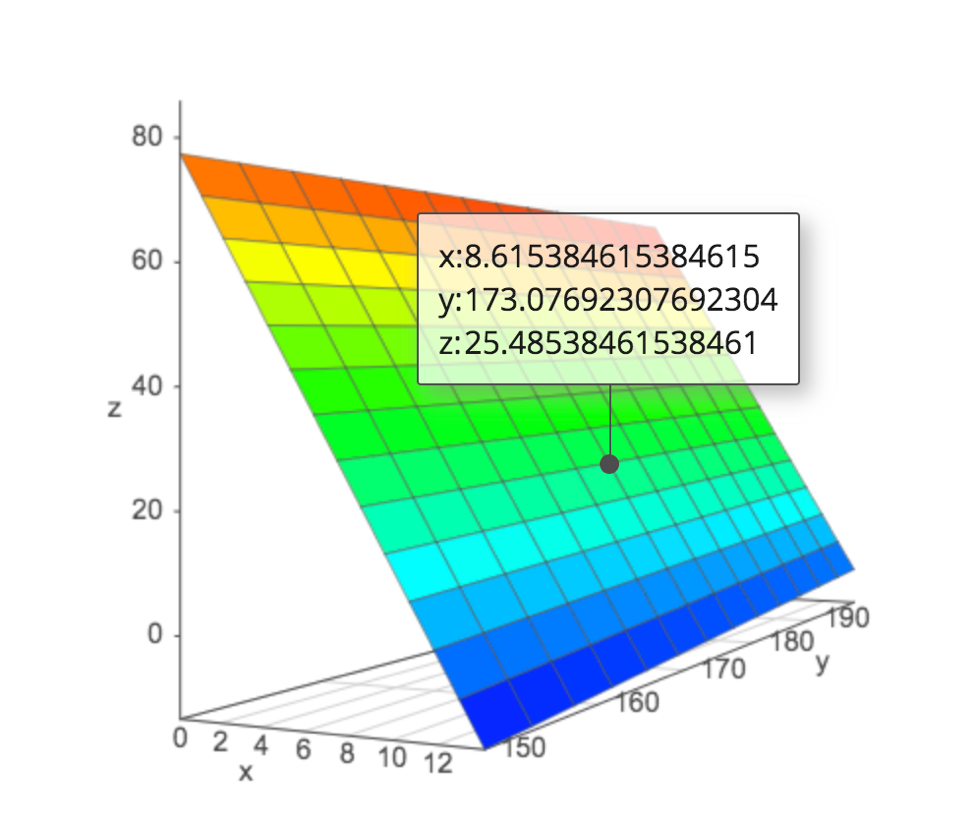
\includegraphics[width=0.4\linewidth]{Plane}

We can further explore the regression plane a
\href{https://academo.org/demos/3d-surface-plotter/?expression=51.89-6.48*x\%2B0.17*y\&xRange=0\%2C\%2B14\&yRange=150\%2C+200\&resolution=21}{academo.org}.

\subsection{Acc060 and Length Model
Interpretations}\label{acc060-and-length-model-interpretations}

\(\widehat{Price} = b_0 + b_1\times\text{Acc. Time} + b_2\times\text{Length}\)

\(\widehat{Price} = 51.83936 + -6.48340\times\text{Acc. Time} + 0.17316\times\text{Length}\)

\begin{itemize}
\item
  Intercept \(b_0\) might be interpreted as the price of a car that can
  accelerate from 0 to 60 in no time and has length 0, but this is not a
  meaningful interpretation since there are no such cars.
\item
  \(b_1=-6.4834\) tells us that on average, the price of a car is
  expected to decrease by 6.48 thousand dollars for each additional
  second it takes to accelerate from 0 to 60 mph., assuming length is
  held constant.
\item
  \(b_2=0.17316\) tells us that on average, the price of a car is
  expected to increase by 0.173 thousand dollars (or \(173\)) for each
  additional inch in length, assuming the time it takes to accelerate
  from 0 to 60 mph. is held constant.
\item
  \(R^2 = 0.5715\) tells us that 57\% of the variation in price is
  explained by the linear model using acceleration time and length as
  the explanatory variables.
\end{itemize}

\subsection{Modeling Price using Acc060 and Length with
Interaction}\label{modeling-price-using-acc060-and-length-with-interaction}

\(\widehat{Price} = b_0 + b_1\times\text{Acc. Time} + b_2\times\text{Length}+ b_3\times\text{Acc. Time}\times\text{Length}\)

\textbf{Model Assumptions:}

\begin{itemize}
\item
  Assumes expected price is a linear function of acceleration time and
  length.
\item
  Assumes that rate of increase in expected price increases with respect
  to acc. time differs depending on length of the car.
\item
  Assumes that rate of increase in expected price increases with respect
  to length differs depending on acceleration time of the car.
\end{itemize}

\subsection{Predictions using Price, Acc060, Length Model with
Interaction}\label{predictions-using-price-acc060-length-model-with-interaction}

\(\widehat{Price} = b_0 + b_1\times\text{Acc. Time} + b_2\times\text{Length} + b_3\times\text{Acc. Time}\times\text{Length}\)

Predicted Price for 150 inch car:

\[
\begin{aligned}
\widehat{Price} & = b_0 + b_1\times\text{Acc. Time} + b_2\times150 + b_3\times\text{Acc. Time}\times150 \\
 &= (b_0 + 150b_2) + (b_1+150b_3)\times\text{Acc. Time}
\end{aligned}
\]

Predicted Price for 200 inch car:

\[
\begin{aligned}
\widehat{Price} & = b_0 + b_1\times\text{Acc. Time} + b_2\times 200 + b_3\times\text{Acc. Time}\times 200 \\
 &= (b_0 + 200b_2) + (b_1+200b_3)\times\text{Acc. Time}
\end{aligned}
\]

\subsection{Interaction Model for Quantitative
Variables}\label{interaction-model-for-quantitative-variables}

We specify an interaction model in R using the \texttt{*} between the
explanatory variables.

\begin{Shaded}
\begin{Highlighting}[]
\NormalTok{Cars_M_A060_L_Int <-}\StringTok{ }\KeywordTok{lm}\NormalTok{(}\DataTypeTok{data=}\NormalTok{Cars2015, LowPrice }\OperatorTok{~}\StringTok{ }\NormalTok{Acc060 }\OperatorTok{*}\StringTok{ }\NormalTok{Length)}
\KeywordTok{summary}\NormalTok{(Cars_M_A060_L_Int)}
\end{Highlighting}
\end{Shaded}

\begin{verbatim}
## 
## Call:
## lm(formula = LowPrice ~ Acc060 * Length, data = Cars2015)
## 
## Residuals:
##      Min       1Q   Median       3Q      Max 
## -31.0782  -5.2974  -0.6007   4.2479  31.3622 
## 
## Coefficients:
##                 Estimate Std. Error t value  Pr(>|t|)    
## (Intercept)   -160.25438   54.11260  -2.961   0.00378 ** 
## Acc060          19.00490    6.21545   3.058   0.00282 ** 
## Length           1.34893    0.29447   4.581 0.0000127 ***
## Acc060:Length   -0.14260    0.03459  -4.123 0.0000745 ***
## ---
## Signif. codes:  0 '***' 0.001 '**' 0.01 '*' 0.05 '.' 0.1 ' ' 1
## 
## Residual standard error: 9.814 on 106 degrees of freedom
## Multiple R-squared:  0.6307, Adjusted R-squared:  0.6203 
## F-statistic: 60.35 on 3 and 106 DF,  p-value: < 0.00000000000000022
\end{verbatim}

\subsection{Cars Interaction Model
Interpretations}\label{cars-interaction-model-interpretations}

\(\widehat{Price} = -160.25438 + 19.00490\times\text{Acc. Time} + 1.34893\times\text{Length} - 0.14260\times\text{Acc. Time}\times\text{Length}\)

For a car that is 150 inches long:

\[
\begin{aligned}
\widehat{Price} & = -160.25438 + 19.00490\times\text{Acc. Time} + 1.34893\times150 - 0.14260\times\text{Acc. Time}\times150 \\
 &= 42.085 -2.385\times\text{Acc. Time} 
\end{aligned}
\]

For a 150 inch car, price is expected to decrease by 2.385 thousand
dollars for each additional second it takes to accelerate from 0 to 60
mph.

\[
\begin{aligned}
\widehat{Price} & = -160.25438 + 19.00490\times\text{Acc. Time} + 1.34893\times200 - 0.14260\times\text{Acc. Time}\times200 \\
 &= 109.532 -9.515\times\text{Acc. Time} 
\end{aligned}
\]

For a 200 inch car, price is expected to decrease by 9.515 thousand
dollars for each additional second it takes to accelerate from 0 to 60
mph.

When using an interaction model, we can only interpret coefficients with
respect to one variable for a given value of the other variable.

\(R^2=0.6307\) tells us that 63\% of variation in car price is explained
by the model using length and acceleration time with interaction.

\subsection{\texorpdfstring{Predicting Car Price Using
\texttt{predict}}{Predicting Car Price Using predict}}\label{predicting-car-price-using-predict}

Predict the price of a 200 inch car that can acclerate from 0 to 60 mph
in 8 seconds.

\begin{Shaded}
\begin{Highlighting}[]
\KeywordTok{predict}\NormalTok{(Cars_M_A060_L_Int, }\DataTypeTok{newdata=}\KeywordTok{data.frame}\NormalTok{(}\DataTypeTok{Acc060=}\DecValTok{8}\NormalTok{, }\DataTypeTok{Length=}\DecValTok{200}\NormalTok{))}
\end{Highlighting}
\end{Shaded}

\begin{verbatim}
##        1 
## 33.40344
\end{verbatim}

Predict the price of a 150 inch car that can acclerate from 0 to 60 mph
in 10 seconds.

\begin{Shaded}
\begin{Highlighting}[]
\KeywordTok{predict}\NormalTok{(Cars_M_A060_L_Int, }\DataTypeTok{newdata=}\KeywordTok{data.frame}\NormalTok{(}\DataTypeTok{Acc060=}\DecValTok{10}\NormalTok{, }\DataTypeTok{Length=}\DecValTok{150}\NormalTok{))}
\end{Highlighting}
\end{Shaded}

\begin{verbatim}
##        1 
## 18.22735
\end{verbatim}

\chapter{Interval Estimation via
Simulation}\label{interval-estimation-via-simulation}

\section{Sampling Variability and Margin of
Error}\label{sampling-variability-and-margin-of-error}

\subsection{Sampling Variability}\label{sampling-variability}

\begin{itemize}
\item
  Next, we turn our attention to the topic of quantifying uncertainty
  associated with a sample or experiment performed using random
  assignment.
\item
  Our goal is to generalize results to a larger population.
\item
  If our sample was collected in a way that is not representative of a
  larger population of interest, then we should be cautious about
  generalizing our results.
\item
  If we already have data about the entire population we are interested
  in, then these results are not relevant.
\end{itemize}

\subsection{Election Polling Example}\label{election-polling-example}

A Washington Post
\href{https://www.washingtonpost.com/context/sept-8-13-2020-washington-post-abc-news-poll-of-minnesota-and-wisconsin/8e5dbd4b-4746-4e45-821e-eb8c8645d5c1/}{poll},
of 702 registered voters in the state of Wisconsin, taken from September
8-13, 2020 showed that:

\begin{itemize}
\tightlist
\item
  50\% intend to vote for Joe Biden\\
\item
  46\% intend to vote for Donald Trump\\
\item
  4\% weren't sure or intend to vote for other candidates
\end{itemize}

Is this strong enough information to say that Joe Biden is ahead among
all voters in Wisconsin? Is it possible that Biden is not really ahead,
and the poll just happened to sample more of his supporters but random
chance?

\subsection{Investigation by
Simulation}\label{investigation-by-simulation}

\textbf{Key Questions:}

By how much could proportions in a random sample of 702 voters plausibly
differ from proportions for all Wisconsin voters?

We'll investigate this using the following steps:

\begin{enumerate}
\def\labelenumi{\arabic{enumi}.}
\tightlist
\item
  Assume we know the percentage of voters in the state supporting each
  candidate.\\
\item
  Simulate taking random samples of 702 voters. Record how far the poll
  result differs from those of the population.
\end{enumerate}

\subsection{Larger Population}\label{larger-population}

\begin{itemize}
\item
  As of August 1, 2020, there were 3,420,587 registered voters in the
  state of Wisconsin.
\item
  We'll assume (hypothetically) that for the upcoming election:

  \begin{itemize}
  \tightlist
  \item
    1,641,882 (48\%) plan to vote for the Biden\\
  \item
    1,641,882 (48\%) plan to vote for the Trump\\
  \item
    136,823 (4\%) plan to vote for a third-party or independent
    candidate
  \end{itemize}
\end{itemize}

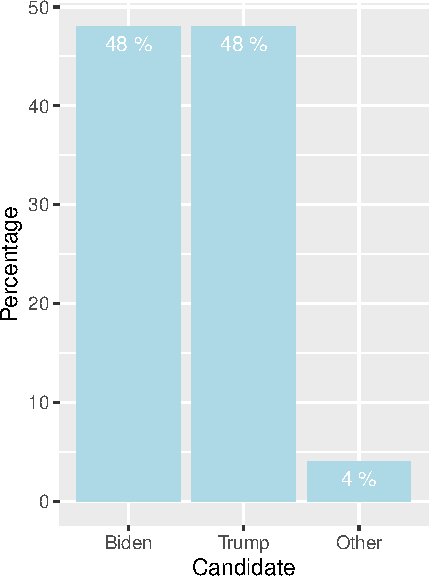
\includegraphics{_main_files/figure-latex/unnamed-chunk-125-1.pdf}

\subsection{A sample of 702 voters}\label{a-sample-of-702-voters}

\begin{Shaded}
\begin{Highlighting}[]
\NormalTok{Vote <-}\StringTok{ }\KeywordTok{factor}\NormalTok{(}\KeywordTok{c}\NormalTok{(}\KeywordTok{rep}\NormalTok{(}\StringTok{"Biden"}\NormalTok{, }\DecValTok{1641882}\NormalTok{), }\KeywordTok{rep}\NormalTok{(}\StringTok{"Trump"}\NormalTok{, }\DecValTok{1641882}\NormalTok{), }\KeywordTok{rep}\NormalTok{(}\StringTok{"Other"}\NormalTok{, }\DecValTok{136823}\NormalTok{))) }
\NormalTok{Population <-}\StringTok{ }\KeywordTok{as.data.frame}\NormalTok{(Vote)}
\end{Highlighting}
\end{Shaded}

\begin{Shaded}
\begin{Highlighting}[]
\NormalTok{Sample <-}\StringTok{ }\KeywordTok{sample_n}\NormalTok{(Population, }\DecValTok{702}\NormalTok{, }\DataTypeTok{replace=}\OtherTok{FALSE}\NormalTok{)}
\end{Highlighting}
\end{Shaded}

Population Summary:

\begin{Shaded}
\begin{Highlighting}[]
\KeywordTok{summary}\NormalTok{(Population}\OperatorTok{$}\NormalTok{Vote)}
\end{Highlighting}
\end{Shaded}

\begin{verbatim}
##   Biden   Other   Trump 
## 1641882  136823 1641882
\end{verbatim}

Results in random sample of 702 voters:

\begin{Shaded}
\begin{Highlighting}[]
\KeywordTok{summary}\NormalTok{(Sample}\OperatorTok{$}\NormalTok{Vote)}
\end{Highlighting}
\end{Shaded}

\begin{verbatim}
## Biden Other Trump 
##   330    31   341
\end{verbatim}

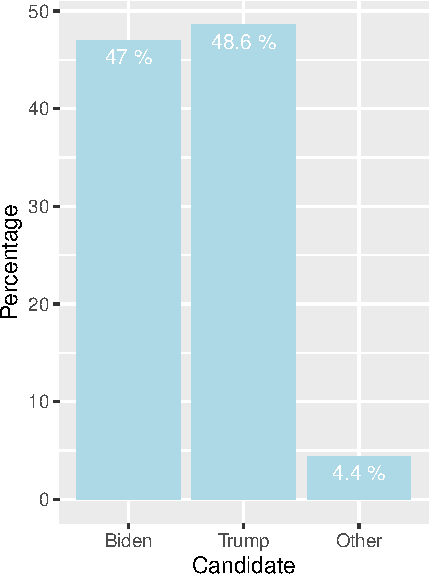
\includegraphics{_main_files/figure-latex/unnamed-chunk-131-1.pdf}

\subsection{A Second Sample of 702
Voters}\label{a-second-sample-of-702-voters}

Let's simulate taking another random sample of 702 voters.

\begin{Shaded}
\begin{Highlighting}[]
\NormalTok{Sample <-}\StringTok{ }\KeywordTok{sample_n}\NormalTok{(Population, }\DecValTok{702}\NormalTok{, }\DataTypeTok{replace=}\OtherTok{FALSE}\NormalTok{)}
\end{Highlighting}
\end{Shaded}

Population Summary:

\begin{Shaded}
\begin{Highlighting}[]
\KeywordTok{summary}\NormalTok{(Population}\OperatorTok{$}\NormalTok{Vote)}
\end{Highlighting}
\end{Shaded}

\begin{verbatim}
##   Biden   Other   Trump 
## 1641882  136823 1641882
\end{verbatim}

Results in random sample of 702 voters:

\begin{Shaded}
\begin{Highlighting}[]
\KeywordTok{summary}\NormalTok{(Sample}\OperatorTok{$}\NormalTok{Vote)}
\end{Highlighting}
\end{Shaded}

\begin{verbatim}
## Biden Other Trump 
##   333    20   349
\end{verbatim}

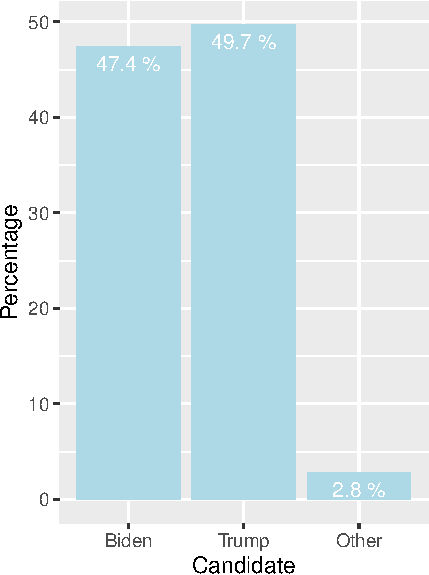
\includegraphics{_main_files/figure-latex/unnamed-chunk-135-1.pdf}

\subsection{A Third Sample of 702
Voters}\label{a-third-sample-of-702-voters}

Let's simulate taking another third random sample of 702 voters.

\begin{Shaded}
\begin{Highlighting}[]
\NormalTok{Sample <-}\StringTok{ }\KeywordTok{sample_n}\NormalTok{(Population, }\DecValTok{702}\NormalTok{, }\DataTypeTok{replace=}\OtherTok{FALSE}\NormalTok{)}
\end{Highlighting}
\end{Shaded}

Population Summary:

\begin{Shaded}
\begin{Highlighting}[]
\KeywordTok{summary}\NormalTok{(Population}\OperatorTok{$}\NormalTok{Vote)}
\end{Highlighting}
\end{Shaded}

\begin{verbatim}
##   Biden   Other   Trump 
## 1641882  136823 1641882
\end{verbatim}

Results in random sample of 702 voters:

\begin{Shaded}
\begin{Highlighting}[]
\KeywordTok{summary}\NormalTok{(Sample}\OperatorTok{$}\NormalTok{Vote)}
\end{Highlighting}
\end{Shaded}

\begin{verbatim}
## Biden Other Trump 
##   341    28   333
\end{verbatim}

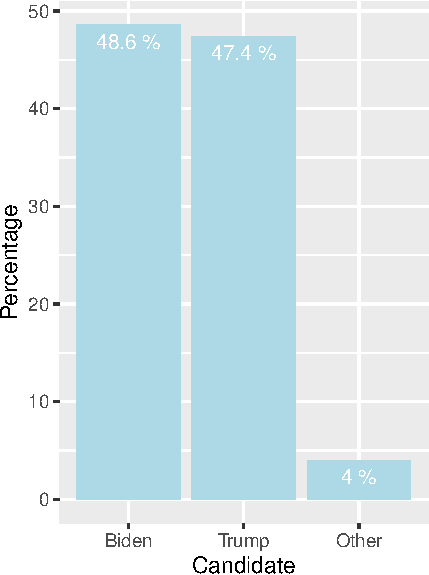
\includegraphics{_main_files/figure-latex/unnamed-chunk-139-1.pdf}

\subsection{A Fourth Sample of 702
Voters}\label{a-fourth-sample-of-702-voters}

Let's simulate taking another fourth random sample of 702 voters.

\begin{Shaded}
\begin{Highlighting}[]
\NormalTok{Sample <-}\StringTok{ }\KeywordTok{sample_n}\NormalTok{(Population, }\DecValTok{702}\NormalTok{, }\DataTypeTok{replace=}\OtherTok{FALSE}\NormalTok{)}
\end{Highlighting}
\end{Shaded}

Population Summary:

\begin{Shaded}
\begin{Highlighting}[]
\KeywordTok{summary}\NormalTok{(Population}\OperatorTok{$}\NormalTok{Vote)}
\end{Highlighting}
\end{Shaded}

\begin{verbatim}
##   Biden   Other   Trump 
## 1641882  136823 1641882
\end{verbatim}

Results in random sample of 702 voters:

\begin{Shaded}
\begin{Highlighting}[]
\KeywordTok{summary}\NormalTok{(Sample}\OperatorTok{$}\NormalTok{Vote)}
\end{Highlighting}
\end{Shaded}

\begin{verbatim}
## Biden Other Trump 
##   355    29   318
\end{verbatim}

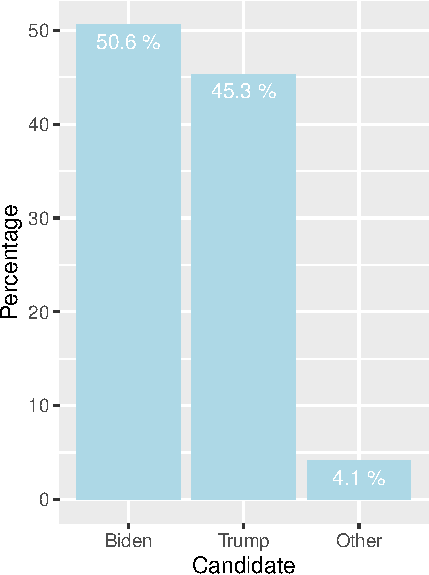
\includegraphics{_main_files/figure-latex/unnamed-chunk-143-1.pdf}

\subsection{A Fifth Sample of 702
Voters}\label{a-fifth-sample-of-702-voters}

Let's simulate taking another fourth random sample of 702 voters.

\begin{Shaded}
\begin{Highlighting}[]
\NormalTok{Sample <-}\StringTok{ }\KeywordTok{sample_n}\NormalTok{(Population, }\DecValTok{702}\NormalTok{, }\DataTypeTok{replace=}\OtherTok{FALSE}\NormalTok{)}
\end{Highlighting}
\end{Shaded}

Population Summary:

\begin{Shaded}
\begin{Highlighting}[]
\KeywordTok{summary}\NormalTok{(Population}\OperatorTok{$}\NormalTok{Vote)}
\end{Highlighting}
\end{Shaded}

\begin{verbatim}
##   Biden   Other   Trump 
## 1641882  136823 1641882
\end{verbatim}

Results in random sample of 702 voters:

\begin{Shaded}
\begin{Highlighting}[]
\KeywordTok{summary}\NormalTok{(Sample}\OperatorTok{$}\NormalTok{Vote)}
\end{Highlighting}
\end{Shaded}

\begin{verbatim}
## Biden Other Trump 
##   315    24   363
\end{verbatim}

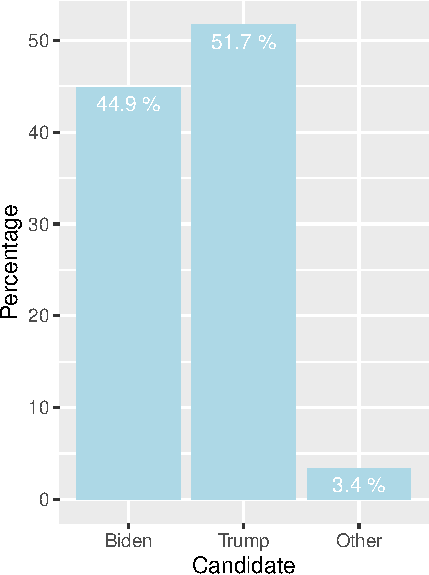
\includegraphics{_main_files/figure-latex/unnamed-chunk-147-1.pdf}

\subsection{Simulating Many Polls}\label{simulating-many-polls}

Let's simulate 10,000 different polls of 702 voters and look at how much
variability we see in the difference in proportions supporting each
candidate.

\begin{Shaded}
\begin{Highlighting}[]
\KeywordTok{set.seed}\NormalTok{(}\DecValTok{09132020}\NormalTok{)}
\end{Highlighting}
\end{Shaded}

\begin{Shaded}
\begin{Highlighting}[]
\NormalTok{Biden <-}\StringTok{ }\KeywordTok{rep}\NormalTok{(}\OtherTok{NA}\NormalTok{, }\DecValTok{10000}\NormalTok{) }\CommentTok{#blank vector to store proportion supporting Biden}
\NormalTok{Trump <-}\StringTok{ }\KeywordTok{rep}\NormalTok{(}\OtherTok{NA}\NormalTok{, }\DecValTok{10000}\NormalTok{) }\CommentTok{#blank vector to store proportion supporting Trump}
\NormalTok{Other <-}\StringTok{ }\KeywordTok{rep}\NormalTok{(}\OtherTok{NA}\NormalTok{, }\DecValTok{10000}\NormalTok{) }\CommentTok{#blank vector to store proportion supporting Other}

\ControlFlowTok{for}\NormalTok{ (i }\ControlFlowTok{in} \DecValTok{1}\OperatorTok{:}\DecValTok{10000}\NormalTok{)\{}
\NormalTok{Sample <-}\StringTok{ }\KeywordTok{sample_n}\NormalTok{(Population, }\DecValTok{702}\NormalTok{, }\DataTypeTok{replace=}\OtherTok{FALSE}\NormalTok{)  }\CommentTok{#sample 1000 voters}
\NormalTok{Biden[i] <-}\StringTok{ }\KeywordTok{sum}\NormalTok{(Sample }\OperatorTok{==}\StringTok{ "Biden"}\NormalTok{)}\OperatorTok{/}\DecValTok{702}\NormalTok{   ## record number of Biden votes}
\NormalTok{Trump[i] <-}\StringTok{ }\KeywordTok{sum}\NormalTok{(Sample }\OperatorTok{==}\StringTok{ "Trump"}\NormalTok{)}\OperatorTok{/}\DecValTok{702}\NormalTok{   ## record number of Trump votes}
\NormalTok{Other[i] <-}\StringTok{ }\KeywordTok{sum}\NormalTok{(Sample }\OperatorTok{==}\StringTok{ "Other"}\NormalTok{)}\OperatorTok{/}\DecValTok{702}\NormalTok{   ## record number of Other votes}
\NormalTok{\}}

\NormalTok{Sim <-}\StringTok{ }\DecValTok{1}\OperatorTok{:}\DecValTok{10000}
\NormalTok{PollingSim <-}\StringTok{ }\KeywordTok{data.frame}\NormalTok{(Sim, Biden, Trump, Other)}
\NormalTok{PollingSim}\OperatorTok{$}\NormalTok{PropDiff <-}\StringTok{ }\NormalTok{PollingSim}\OperatorTok{$}\NormalTok{Biden}\OperatorTok{-}\NormalTok{PollingSim}\OperatorTok{$}\NormalTok{Trump}
\end{Highlighting}
\end{Shaded}

\subsection{Histogram of Difference in Sample
Proportions}\label{histogram-of-difference-in-sample-proportions}

The histogram shows the difference in proportion favoring each party's
candidate in the 10,000 samples.

Recall that the samples were taken under the assumption that there is no
difference in support between the Republican or Democrat in the
population.

\begin{Shaded}
\begin{Highlighting}[]
\NormalTok{Vote_Samp_Dist <-}\StringTok{ }\KeywordTok{ggplot}\NormalTok{(}\DataTypeTok{data=}\NormalTok{PollingSim, }\KeywordTok{aes}\NormalTok{(}\DataTypeTok{x=}\NormalTok{PropDiff)) }\OperatorTok{+}\StringTok{  }\KeywordTok{geom_histogram}\NormalTok{(}\DataTypeTok{fill=}\StringTok{"blue"}\NormalTok{, }\DataTypeTok{color=}\StringTok{"white"}\NormalTok{, }\DataTypeTok{binwidth=}\FloatTok{0.001}\NormalTok{) }\OperatorTok{+}\StringTok{ }
\StringTok{  }\KeywordTok{xlab}\NormalTok{(}\StringTok{" Dem. Prop. - Rep. Prop"}\NormalTok{) }\OperatorTok{+}\StringTok{ }\KeywordTok{ylab}\NormalTok{(}\StringTok{"Frequency"}\NormalTok{) }\OperatorTok{+}\StringTok{ }
\StringTok{  }\KeywordTok{ggtitle}\NormalTok{(}\StringTok{"Sampling Distribution for Difference in Proportions"}\NormalTok{)}
\NormalTok{Vote_Samp_Dist }
\end{Highlighting}
\end{Shaded}

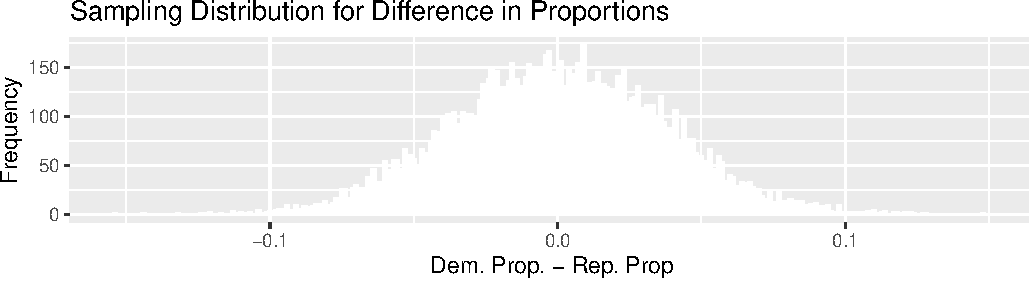
\includegraphics{_main_files/figure-latex/unnamed-chunk-150-1.pdf}

This distribution is called the \textbf{sampling distribution} for the
difference in proportions.

\subsection{Sampling Dist. for Diff. in
Proportions}\label{sampling-dist.-for-diff.-in-proportions}

\includegraphics{_main_files/figure-latex/unnamed-chunk-151-1.pdf}

\begin{Shaded}
\begin{Highlighting}[]
\KeywordTok{mean}\NormalTok{(PollingSim}\OperatorTok{$}\NormalTok{PropDiff)}
\end{Highlighting}
\end{Shaded}

\begin{verbatim}
## [1] 0.0003595442
\end{verbatim}

\begin{Shaded}
\begin{Highlighting}[]
\NormalTok{SE <-}\StringTok{ }\KeywordTok{sd}\NormalTok{(PollingSim}\OperatorTok{$}\NormalTok{PropDiff)}
\NormalTok{SE}
\end{Highlighting}
\end{Shaded}

\begin{verbatim}
## [1] 0.03689199
\end{verbatim}

The sampling distribution for the difference in candidate support is
approximately centered at 0, as we would expect. The standard deviation
in difference between candidates is about 3.7 percentage points.

\subsection{Difference in Sample Proportions
(cont.)}\label{difference-in-sample-proportions-cont.}

\includegraphics{_main_files/figure-latex/unnamed-chunk-154-1.pdf}

\begin{Shaded}
\begin{Highlighting}[]
\KeywordTok{c}\NormalTok{(}\KeywordTok{quantile}\NormalTok{(PollingSim}\OperatorTok{$}\NormalTok{PropDiff, .}\DecValTok{025}\NormalTok{), }\KeywordTok{quantile}\NormalTok{(PollingSim}\OperatorTok{$}\NormalTok{PropDiff, .}\DecValTok{975}\NormalTok{))}
\end{Highlighting}
\end{Shaded}

\begin{verbatim}
##        2.5%       97.5% 
## -0.07122507  0.07264957
\end{verbatim}

\begin{itemize}
\tightlist
\item
  Approximately 95\% of the polls were within \(\pm 7\) of the actual
  difference, which in this case was assumed to be 0.
\end{itemize}

\subsection{Conclusions from Election Polling
Simulation}\label{conclusions-from-election-polling-simulation}

Since Biden is ahead by 4 percentage points in the Washington Post
survey of 702 voters, it is plausible that he could really be ahead by
as many as about 11 percentage points, or behind by as many as about 3.

\begin{itemize}
\item
  The \(\pm .07\) is called a \textbf{margin of error}, and the
  resulting range of plausible values is called a \textbf{confidence
  interval} for the difference in proportions.
\item
  A confidence interval gives a reasonable range for a value pertaining
  to the entire population, using information from a sample.
\end{itemize}

\subsection{\texorpdfstring{What does ``95\% Confidence''
Mean?}{What does 95\% Confidence Mean?}}\label{what-does-95-confidence-mean}

95\% confidence means that if we were to repeat our procedure on many,
random samples, then in the long run, 95\% of them would contain the
true difference in proportions supporting the candidates.

\includegraphics{_main_files/figure-latex/unnamed-chunk-157-1.pdf}

Here, we see results for 100 random samples. Notice that when we do
\(\text{Prop. Diff} \pm 0.07\), approximately 95\% lead to a confidence
interval containing 0 (the assumed true difference).

\section{Bootstrap Sampling for Election
Example}\label{bootstrap-sampling-for-election-example}

\subsection{A More Realistic Scenario}\label{a-more-realistic-scenario}

\begin{itemize}
\item
  The prior simulation is based on the unrealistic assumption that we
  know the proportion of voters in the entire population favoring each
  candidate.
\item
  If we really know this, there would be no need to take polls.
\item
  In reality, we will only have the result of a single sample, and from
  that, we will need to determine how much our result might vary from
  the overall population parameter.
\end{itemize}

\subsection{Example: Election Polling
Survey}\label{example-election-polling-survey}

Recall the Washington Post Poll of 702 Wisconsin voters that showed 50\%
supporting Biden, and 46\% supporting Trump.

Although the poll does not release exact counts, we can infer that 351
voters picked Biden, 323 picked Trump, and 28 picked someone else.

Without assuming anything about the larger population, how can we
account for sampling variability to obtain a reasonable range for the
true difference in proportion of voters supporting the candidates?

\subsection{\texorpdfstring{Illustration of the Bootstrap
``Idea''}{Illustration of the Bootstrap Idea}}\label{illustration-of-the-bootstrap-idea}

Bootstrap sampling is a popular modern approach for measuring sampling
variability.

The idea is to mimic sampling from a population, by copying the sample
many times, and then sampling from these copies.

\includegraphics[width=0.5\linewidth]{Bootstrap_Idea}

We then calculate the statistic of interest (i.e.~difference in
proportions) in each bootstrap sample to get a sense of the amount of
variability between samples.

\subsection{\texorpdfstring{The Bootstrap
``Idea''}{The Bootstrap Idea}}\label{the-bootstrap-idea}

\begin{enumerate}
\def\labelenumi{\arabic{enumi}.}
\item
  Create many (theoretically infinitely many) copies of the original
  sample.
\item
  Take a sample of the same size as our original sample. This is known
  as a \textbf{bootstrap sample.} Since we have created many copies of
  the original sample some cases will come up multiple times and others
  not at all in our bootstrap sample.
\item
  Calculate the difference in proportions supporting each candidate in
  the bootstrap sample.
\item
  Repeat steps 2 and 3 many (say 10,000) times, keeping track of the
  differences in proportions supporting each candidate.
\item
  Look at the distribution of differences calculated from the bootstrap
  samples. The variability in this distribution can be used to
  approximate the variability in the sampling distribution for the
  difference in proportions.
\end{enumerate}

\subsection{Bootstrap via Resampling
Illustration}\label{bootstrap-via-resampling-illustration}

Copying the original sample infinitely many times, and then sampling
from these copies is equivalent to simply sampling from the original
sample, using replacement. This is how bootstrap sampling is done in
practice.

\includegraphics[width=0.7\linewidth]{Bootstrap}

\subsection{Bootstrap Sampling with
Replacement}\label{bootstrap-sampling-with-replacement}

In practice, the bootstrap is performed by resampling from the original
data, with replacement.

\textbf{Procedure:}

\begin{enumerate}
\def\labelenumi{\arabic{enumi}.}
\item
  Take a sample of the same size as our original sample, by sampling
  cases from the original sample, with replacement. Since are sampling
  with replacement, some cases will come up multiple times and others
  not at all in our bootstrap sample.
\item
  Calculate the difference in proportions supporting each candidate in
  the bootstrap sample.
\item
  Repeat steps 2 and 3 many (say 10,000) times, keeping track of the
  differences in proportions supporting each candidate.
\item
  Look at the distribution of differences calculated from the bootstrap
  samples. The variability in this distribution can be used to
  approximate the variability in the sampling distribution for the
  difference in proportions.
\end{enumerate}

\subsection{Code for Bootstrapping for Difference In
Proportions}\label{code-for-bootstrapping-for-difference-in-proportions}

\begin{Shaded}
\begin{Highlighting}[]
\NormalTok{Vote <-}\StringTok{ }\KeywordTok{c}\NormalTok{(}\KeywordTok{rep}\NormalTok{(}\StringTok{"Biden"}\NormalTok{, }\DecValTok{351}\NormalTok{), }\KeywordTok{rep}\NormalTok{(}\StringTok{"Trump"}\NormalTok{, }\DecValTok{323}\NormalTok{), }\KeywordTok{rep}\NormalTok{(}\StringTok{"Other"}\NormalTok{, }\DecValTok{28}\NormalTok{))}
\NormalTok{Sample <-}\StringTok{ }\KeywordTok{data.frame}\NormalTok{(Vote)}

\NormalTok{Difference <-}\StringTok{ }\KeywordTok{rep}\NormalTok{(}\OtherTok{NA}\NormalTok{, }\DecValTok{10000}\NormalTok{)}
\ControlFlowTok{for}\NormalTok{ (i }\ControlFlowTok{in} \DecValTok{1}\OperatorTok{:}\DecValTok{10000}\NormalTok{)\{}
\NormalTok{BootstrapSample <-}\StringTok{ }\KeywordTok{sample_n}\NormalTok{(Sample, }\DecValTok{702}\NormalTok{, }\DataTypeTok{replace=}\OtherTok{TRUE}\NormalTok{) }
\NormalTok{Difference[i] <-}\StringTok{ }\NormalTok{(}\KeywordTok{sum}\NormalTok{(BootstrapSample}\OperatorTok{$}\NormalTok{Vote}\OperatorTok{==}\StringTok{"Biden"}\NormalTok{) }\OperatorTok{-}\StringTok{ }\KeywordTok{sum}\NormalTok{(BootstrapSample}\OperatorTok{$}\NormalTok{Vote}\OperatorTok{==}\StringTok{"Trump"}\NormalTok{))}\OperatorTok{/}\DecValTok{702}
\NormalTok{\}}
\NormalTok{Vote_BootstrapResults <-}\StringTok{ }\KeywordTok{data.frame}\NormalTok{(Difference)}
\end{Highlighting}
\end{Shaded}

\subsection{Bootstrap Dist. for Diff. in
Proportion}\label{bootstrap-dist.-for-diff.-in-proportion}

\includegraphics{_main_files/figure-latex/unnamed-chunk-161-1.pdf}

\begin{itemize}
\item
  Note that the bootstrap distibution is centered at approximately 0.04,
  which was the observed difference we saw in our sample.
\item
  Individual sample differences seem to deviate by up to about
  \(\pm 0.07\).
\end{itemize}

\textbf{Bootstrap standard error:}

\begin{Shaded}
\begin{Highlighting}[]
\KeywordTok{sd}\NormalTok{(Vote_BootstrapResults}\OperatorTok{$}\NormalTok{Difference)}
\end{Highlighting}
\end{Shaded}

\begin{verbatim}
## [1] 0.03700877
\end{verbatim}

\subsection{Bootstrap Percentile Confidence
Interval}\label{bootstrap-percentile-confidence-interval}

An approximate 95\% percentile confidence interval for the difference in
support is found by finding the 0.025 and 0.975 quantiles of the
bootstrap distribution, since 95\% of all bootstrap samples produce
statistics between these values.

\begin{Shaded}
\begin{Highlighting}[]
\NormalTok{q.}\DecValTok{025}\NormalTok{ <-}\StringTok{ }\KeywordTok{quantile}\NormalTok{(Vote_BootstrapResults}\OperatorTok{$}\NormalTok{Difference, }\FloatTok{0.025}\NormalTok{)}
\NormalTok{q.}\DecValTok{975}\NormalTok{ <-}\StringTok{ }\KeywordTok{quantile}\NormalTok{(Vote_BootstrapResults}\OperatorTok{$}\NormalTok{Difference, }\FloatTok{0.975}\NormalTok{)}
\end{Highlighting}
\end{Shaded}

\begin{Shaded}
\begin{Highlighting}[]
\KeywordTok{c}\NormalTok{(q.}\DecValTok{025}\NormalTok{, q.}\DecValTok{975}\NormalTok{)}
\end{Highlighting}
\end{Shaded}

\begin{verbatim}
##        2.5%       97.5% 
## -0.03133903  0.11253561
\end{verbatim}

We can be 95\% confident that Biden is between 11.3 percentage points
ahead, and 3.1 percentage points behind.

\subsection{95\% Bootstrap Percentile Confidence Interval
Visually}\label{bootstrap-percentile-confidence-interval-visually}

\includegraphics{_main_files/figure-latex/unnamed-chunk-165-1.pdf}

We can be 95\% confident that Biden is between 11.3 percentage points
ahead, and 3.1 percentage points behind.

\subsection{Bootstrap Standard Error}\label{bootstrap-standard-error}

The \textbf{bootstrap standard error} is the standard deviation of the
bootstrap distribution. It measures the amount of variability in a
statistic (in this cases difference in proportions) between samples of
the given size.

\begin{Shaded}
\begin{Highlighting}[]
\KeywordTok{sd}\NormalTok{(Vote_BootstrapResults}\OperatorTok{$}\NormalTok{Difference)}
\end{Highlighting}
\end{Shaded}

\begin{verbatim}
## [1] 0.03700877
\end{verbatim}

If large number of polls of 702 voters were taken, the standard
deviation in the distribution of the difference in support between Biden
and Trump is estimated to be 0.0370088

\subsection{Standard Error Confidence
Intervals}\label{standard-error-confidence-intervals}

\begin{itemize}
\item
  Standard error is the standard deviation of the distribution of a
  statistic, across many samples of the given size.
\item
  When the sampling distribution of a statistic is symmetric and
  bell-shaped, then an approximately 95\% of all samples will lead to a
  statistic that is within 2 standard errors of the desired population
  quantity.
\item
  An approximate 95\% bootstrap standard error formula is given by:
\end{itemize}

\[
\text{Statistic} \pm 2\times\text{Standard Error}
\]

\begin{itemize}
\tightlist
\item
  it is only appropriate to use the bootstrap standard error confidence
  interval method when a sampling distribution is symmetric and
  bell-shaped
\end{itemize}

\subsection{Bootstrap Standard Error Confidence
Interval}\label{bootstrap-standard-error-confidence-interval}

\begin{Shaded}
\begin{Highlighting}[]
\NormalTok{SE <-}\StringTok{ }\KeywordTok{sd}\NormalTok{(Vote_BootstrapResults}\OperatorTok{$}\NormalTok{Difference)}
\KeywordTok{c}\NormalTok{(}\FloatTok{0.04} \OperatorTok{-}\StringTok{ }\DecValTok{2}\OperatorTok{*}\NormalTok{SE, }\FloatTok{0.04} \OperatorTok{+}\StringTok{ }\DecValTok{2}\OperatorTok{*}\NormalTok{SE)}
\end{Highlighting}
\end{Shaded}

\begin{verbatim}
## [1] -0.03401753  0.11401753
\end{verbatim}

We can be 95\% confident that Biden is between 11.4 percentage points
ahead, and 3.4 percentage points behind.

The bootstrap percentile confidence interval and bootstrap standard
error confidence intervals largely agree, which we expect to happen when
the bootstrap distribution is symmetric and bell-shaped.

\subsection{Comparison of Bootstrap Confidence
Intervals}\label{comparison-of-bootstrap-confidence-intervals}

\begin{itemize}
\item
  A 95\% bootstrap percentile confidence interval is determined by
  finding the 0.025 and 0.975 quantiles of the bootstrap distribution
  (i.e.~by taking the middle 95\% of the distribution).
\item
  A 95\% standard error confidence interval is determined using
\end{itemize}

\[ \text{Statistic} \pm 2\times\text{Standard Error}
\]

When the bootstrap distribution is symmetric and bell-shaped, these
intervals will be approximately the same.

\subsection{90\% Bootstrap Percentile Confidence
Interval}\label{bootstrap-percentile-confidence-interval-1}

\begin{Shaded}
\begin{Highlighting}[]
\NormalTok{q.}\DecValTok{05}\NormalTok{ <-}\StringTok{ }\KeywordTok{quantile}\NormalTok{(Vote_BootstrapResults}\OperatorTok{$}\NormalTok{Difference, }\FloatTok{0.05}\NormalTok{)}
\NormalTok{q.}\DecValTok{95}\NormalTok{ <-}\StringTok{ }\KeywordTok{quantile}\NormalTok{(Vote_BootstrapResults}\OperatorTok{$}\NormalTok{Difference, }\FloatTok{0.95}\NormalTok{)}
\end{Highlighting}
\end{Shaded}

\begin{Shaded}
\begin{Highlighting}[]
\KeywordTok{c}\NormalTok{(q.}\DecValTok{05}\NormalTok{, q.}\DecValTok{95}\NormalTok{)}
\end{Highlighting}
\end{Shaded}

\begin{verbatim}
##          5%         95% 
## -0.02136752  0.10113960
\end{verbatim}

We can be 90\% confident that Biden is between 10 percentage points
ahead, and 2 percentage points behind.

\subsection{90\% Bootstrap Confidence Interval
Visually}\label{bootstrap-confidence-interval-visually}

\includegraphics{_main_files/figure-latex/unnamed-chunk-170-1.pdf}

We can be 90\% confident that Biden is between 10 percentage points
ahead, and 2 percentage points behind.

\subsection{Comments on Election
Polling}\label{comments-on-election-polling}

\begin{itemize}
\item
  In reality, it is very hard to obtain a ``random'' sample of voters.
  Voters can be hard to reach, and many people do not respond to polls.
  Often it is people with the strongest opinions who do. Furthermore,
  some demographic groups are harder to contact than others, and these
  groups are likely to be underrepresented in surveys.
\item
  In order to account for sampling challenges, pollsters tend to weight
  responses so that their proportions match those of registered voters.
  For example, if fewer college students respond to the survey, then
  those that do are weighted more heavily to make up for it.
\item
  Weighting helps offset underrepresentation, but creates additional
  challenges. It is not always clear what weights to use. This is
  especially tricky for election polling, since the demographic
  breakdown of voters who turn out differs from election to election.
\item
  Because of these challenges, polling involves a ``practical'' margin
  of error, in addition to the ``mathematical'' margin of error.
\item
  Political analysts such as those at {[}fivethirtyeight.com{]}
  (\url{https://fivethirtyeight.com/}), average results from many
  different polls to effectively obtain larger samples. This reduces the
  ``mathematical'' margin of error, but the ``practical'' margin of
  error remains.
\item
  Historically, election polling in the United States has been fairly
  accurate (usually within \(\pm 5\) percentage points of the polling
  average) in major national or statwide elections. Polling has proven
  more challenging and sometimes resulted in larger errors in the UK and
  other countries.
\end{itemize}

\section{Bootstrapping Distribution of Sample
Mean}\label{bootstrapping-distribution-of-sample-mean}

\subsection{General Bootstrapping
Procedure}\label{general-bootstrapping-procedure}

The bootstrap procedure can be applied to quantify uncertainty
associated with a wide range of statistics (for example, sample
proportions, means, medians, standard deviations, regression
coefficients, F-statistics, etc.)

Given a statistic that was calculated from a sample\ldots{}

\textbf{Procedure:}

\begin{enumerate}
\def\labelenumi{\arabic{enumi}.}
\item
  Take a sample of the same size as the original sample, by sampling
  cases from the original sample, with replacement.
\item
  Calculate the statistic of interest in the bootstrap sample.
\item
  Repeat steps 2 and 3 many (say 10,000) times, keeping track of the
  statistic calculated in each bootstrap sample.
\item
  Look at the distribution of statistics calculated from the bootstrap
  samples. The variability in this distribution can be used to
  approximate the variability in the sampling distribution for the
  statistic of interest.
\end{enumerate}

\subsection{Bootstrap Illustration}\label{bootstrap-illustration}

\includegraphics[width=1\linewidth]{Bootstrap}

\subsection{Mercury Levels in Florida
Lakes}\label{mercury-levels-in-florida-lakes}

A 2004 study by Lange, T., Royals, H. and Connor, L. examined Mercury
accumulation in large-mouth bass, taken from a sample of 53 Florida
Lakes. If Mercury accumulation exceeds 0.5 ppm, then there are
environmental concerns. In fact, the legal safety limit in Canada is 0.5
ppm, although it is 1 ppm in the United States.

\begin{figure}
\includegraphics[width=0.5\linewidth]{Bass} \caption{https://www.maine.gov/ifw/fish-wildlife/fisheries/species-information/largemouth-bass.html}\label{fig:Bass}
\end{figure}

\subsection{Florida Lakes Dataset}\label{florida-lakes-dataset}

\begin{Shaded}
\begin{Highlighting}[]
\KeywordTok{data}\NormalTok{(}\StringTok{"FloridaLakes"}\NormalTok{)}
\KeywordTok{glimpse}\NormalTok{(FloridaLakes)}
\end{Highlighting}
\end{Shaded}

\begin{verbatim}
## Rows: 53
## Columns: 12
## $ ID                <int> 1, 2, 3, 4, 5, 6, 7, 8, 9, 10, 11, 12, 13, 14, 15, 1~
## $ Lake              <chr> "Alligator", "Annie", "Apopka", "Blue Cypress", "Bri~
## $ Alkalinity        <dbl> 5.9, 3.5, 116.0, 39.4, 2.5, 19.6, 5.2, 71.4, 26.4, 4~
## $ pH                <dbl> 6.1, 5.1, 9.1, 6.9, 4.6, 7.3, 5.4, 8.1, 5.8, 6.4, 5.~
## $ Calcium           <dbl> 3.0, 1.9, 44.1, 16.4, 2.9, 4.5, 2.8, 55.2, 9.2, 4.6,~
## $ Chlorophyll       <dbl> 0.7, 3.2, 128.3, 3.5, 1.8, 44.1, 3.4, 33.7, 1.6, 22.~
## $ AvgMercury        <dbl> 1.23, 1.33, 0.04, 0.44, 1.20, 0.27, 0.48, 0.19, 0.83~
## $ NumSamples        <int> 5, 7, 6, 12, 12, 14, 10, 12, 24, 12, 12, 12, 7, 43, ~
## $ MinMercury        <dbl> 0.85, 0.92, 0.04, 0.13, 0.69, 0.04, 0.30, 0.08, 0.26~
## $ MaxMercury        <dbl> 1.43, 1.90, 0.06, 0.84, 1.50, 0.48, 0.72, 0.38, 1.40~
## $ ThreeYrStdMercury <dbl> 1.53, 1.33, 0.04, 0.44, 1.33, 0.25, 0.45, 0.16, 0.72~
## $ AgeData           <int> 1, 0, 0, 0, 1, 1, 1, 1, 1, 1, 1, 1, 1, 1, 0, 1, 1, 1~
\end{verbatim}

\subsection{Mercury Level in Sample of 53 Florida
Lakes}\label{mercury-level-in-sample-of-53-florida-lakes}

\begin{verbatim}
##               Lake AvgMercury
##          Alligator       1.23
##              Annie       1.33
##             Apopka       0.04
##       Blue Cypress       0.44
##              Brick       1.20
##             Bryant       0.27
##             Cherry       0.48
##           Crescent       0.19
##         Deer Point       0.83
##               Dias       0.81
##               Dorr       0.71
##               Down       0.50
##              Eaton       0.49
##  East Tohopekaliga       1.16
##            Farm-13       0.05
##             George       0.15
##            Griffin       0.19
\end{verbatim}

\begin{verbatim}
##          Lake AvgMercury
##        Harney       0.77
##          Hart       1.08
##    Hatchineha       0.98
##       Iamonia       0.63
##     Istokpoga       0.56
##       Jackson       0.41
##     Josephine       0.73
##      Kingsley       0.34
##     Kissimmee       0.59
##     Lochloosa       0.34
##        Louisa       0.84
##    Miccasukee       0.50
##      Minneola       0.34
##        Monroe       0.28
##       Newmans       0.34
##    Ocean Pond       0.87
##  Ocheese Pond       0.56
##    Okeechobee       0.17
\end{verbatim}

\begin{verbatim}
##          Lake AvgMercury
##        Orange       0.18
##   Panasoffkee       0.19
##        Parker       0.04
##        Placid       0.49
##        Puzzle       1.10
##        Rodman       0.16
##      Rousseau       0.10
##       Sampson       0.48
##         Shipp       0.21
##       Talquin       0.86
##        Tarpon       0.52
##  Tohopekaliga       0.65
##      Trafford       0.27
##         Trout       0.94
##  Tsala Apopka       0.40
##          Weir       0.43
##       Wildcat       0.25
##          Yale       0.27
\end{verbatim}

Sample Mean:

\begin{Shaded}
\begin{Highlighting}[]
\KeywordTok{mean}\NormalTok{(FloridaLakes}\OperatorTok{$}\NormalTok{AvgMercury)}
\end{Highlighting}
\end{Shaded}

\begin{verbatim}
## [1] 0.5271698
\end{verbatim}

\subsection{Distribution of Mercury
Levels}\label{distribution-of-mercury-levels}

\includegraphics{_main_files/figure-latex/unnamed-chunk-177-1.pdf}

\begin{verbatim}
## # A tibble: 1 x 5
##   MeanHg MedianHg StDevHG PropOver1     N
##    <dbl>    <dbl>   <dbl>     <dbl> <int>
## 1  0.527     0.48   0.341     0.113    53
\end{verbatim}

\subsection{Bootstrapping for Mean Mercury Level in All
Lakes}\label{bootstrapping-for-mean-mercury-level-in-all-lakes}

In our sample of 53 lakes, the mean mercury level is 0.527 ppm. However,
this was just a random sample of lakes. We are interested in a
confidence interval for the mean mercury level for all Florida Lakes.

\textbf{Bootstrapping Procedure}

\begin{enumerate}
\def\labelenumi{\arabic{enumi}.}
\item
  Take a bootstrap sample of size 53, by sampling lakes with
  replacement.
\item
  Calculate the mean mercury concentration in the bootstrap sample.
\item
  Repeat steps 2 and 3 10,000 times, keeping track of the mean mercury
  concentrations in each bootstrap sample.
\item
  Look at the distribution of mean concentrations from the bootstrap
  samples. The variability in this distribution can be used to
  approximate the variability in the sampling distribution for the
  sample mean.
\end{enumerate}

\subsection{Original Sample}\label{original-sample}

\begin{verbatim}
##               Lake AvgMercury
##          Alligator       1.23
##              Annie       1.33
##             Apopka       0.04
##       Blue Cypress       0.44
##              Brick       1.20
##             Bryant       0.27
##             Cherry       0.48
##           Crescent       0.19
##         Deer Point       0.83
##               Dias       0.81
##               Dorr       0.71
##               Down       0.50
##              Eaton       0.49
##  East Tohopekaliga       1.16
##            Farm-13       0.05
##             George       0.15
##            Griffin       0.19
\end{verbatim}

\begin{verbatim}
##          Lake AvgMercury
##        Harney       0.77
##          Hart       1.08
##    Hatchineha       0.98
##       Iamonia       0.63
##     Istokpoga       0.56
##       Jackson       0.41
##     Josephine       0.73
##      Kingsley       0.34
##     Kissimmee       0.59
##     Lochloosa       0.34
##        Louisa       0.84
##    Miccasukee       0.50
##      Minneola       0.34
##        Monroe       0.28
##       Newmans       0.34
##    Ocean Pond       0.87
##  Ocheese Pond       0.56
##    Okeechobee       0.17
\end{verbatim}

\begin{verbatim}
##          Lake AvgMercury
##        Orange       0.18
##   Panasoffkee       0.19
##        Parker       0.04
##        Placid       0.49
##        Puzzle       1.10
##        Rodman       0.16
##      Rousseau       0.10
##       Sampson       0.48
##         Shipp       0.21
##       Talquin       0.86
##        Tarpon       0.52
##  Tohopekaliga       0.65
##      Trafford       0.27
##         Trout       0.94
##  Tsala Apopka       0.40
##          Weir       0.43
##       Wildcat       0.25
##          Yale       0.27
\end{verbatim}

Sample Mean:

\begin{Shaded}
\begin{Highlighting}[]
\KeywordTok{mean}\NormalTok{(FloridaLakes}\OperatorTok{$}\NormalTok{AvgMercury)}
\end{Highlighting}
\end{Shaded}

\begin{verbatim}
## [1] 0.5271698
\end{verbatim}

\subsection{Five Bootstrap Samples}\label{five-bootstrap-samples}

The \texttt{sample\_n()} function samples the specified number rows from
a data frame, with or without replacement.

\begin{Shaded}
\begin{Highlighting}[]
\NormalTok{BootstrapSample1 <-}\StringTok{ }\KeywordTok{sample_n}\NormalTok{(FloridaLakes, }\DecValTok{53}\NormalTok{, }\DataTypeTok{replace=}\OtherTok{TRUE}\NormalTok{) }\OperatorTok\StringTok{ }\KeywordTok{arrange}\NormalTok{(Lake)}
\end{Highlighting}
\end{Shaded}

\begin{Shaded}
\begin{Highlighting}[]
\NormalTok{BootstrapSample2 <-}\StringTok{ }\KeywordTok{sample_n}\NormalTok{(FloridaLakes, }\DecValTok{53}\NormalTok{, }\DataTypeTok{replace=}\OtherTok{TRUE}\NormalTok{) }\OperatorTok\StringTok{ }\KeywordTok{arrange}\NormalTok{(Lake)}
\end{Highlighting}
\end{Shaded}

\begin{Shaded}
\begin{Highlighting}[]
\NormalTok{BootstrapSample3 <-}\StringTok{ }\KeywordTok{sample_n}\NormalTok{(FloridaLakes, }\DecValTok{53}\NormalTok{, }\DataTypeTok{replace=}\OtherTok{TRUE}\NormalTok{) }\OperatorTok\StringTok{ }\KeywordTok{arrange}\NormalTok{(Lake)}
\end{Highlighting}
\end{Shaded}

\begin{Shaded}
\begin{Highlighting}[]
\NormalTok{BootstrapSample4 <-}\StringTok{ }\KeywordTok{sample_n}\NormalTok{(FloridaLakes, }\DecValTok{53}\NormalTok{, }\DataTypeTok{replace=}\OtherTok{TRUE}\NormalTok{) }\OperatorTok\StringTok{ }\KeywordTok{arrange}\NormalTok{(Lake)}
\end{Highlighting}
\end{Shaded}

\begin{Shaded}
\begin{Highlighting}[]
\NormalTok{BootstrapSample5 <-}\StringTok{ }\KeywordTok{sample_n}\NormalTok{(FloridaLakes, }\DecValTok{53}\NormalTok{, }\DataTypeTok{replace=}\OtherTok{TRUE}\NormalTok{) }\OperatorTok\StringTok{ }\KeywordTok{arrange}\NormalTok{(Lake)}
\end{Highlighting}
\end{Shaded}

\subsection{Bootstrap Sample 1}\label{bootstrap-sample-1}

\begin{verbatim}
##        Lake AvgMercury
##   Alligator       1.23
##       Annie       1.33
##      Apopka       0.04
##      Bryant       0.27
##      Bryant       0.27
##      Cherry       0.48
##      Cherry       0.48
##  Deer Point       0.83
##  Deer Point       0.83
##        Dias       0.81
##        Dias       0.81
##     Farm-13       0.05
##     Farm-13       0.05
##     Farm-13       0.05
##     Griffin       0.19
##        Hart       1.08
##  Hatchineha       0.98
\end{verbatim}

\begin{verbatim}
##        Lake AvgMercury
##  Hatchineha       0.98
##     Iamonia       0.63
##   Istokpoga       0.56
##   Josephine       0.73
##   Josephine       0.73
##    Kingsley       0.34
##    Kingsley       0.34
##   Kissimmee       0.59
##   Kissimmee       0.59
##   Lochloosa       0.34
##  Miccasukee       0.50
##     Newmans       0.34
##     Newmans       0.34
##     Newmans       0.34
##  Okeechobee       0.17
##  Okeechobee       0.17
##      Parker       0.04
##      Parker       0.04
\end{verbatim}

\begin{verbatim}
##          Lake AvgMercury
##        Placid       0.49
##        Rodman       0.16
##      Rousseau       0.10
##       Sampson       0.48
##       Sampson       0.48
##       Sampson       0.48
##       Talquin       0.86
##       Talquin       0.86
##       Talquin       0.86
##        Tarpon       0.52
##         Trout       0.94
##         Trout       0.94
##         Trout       0.94
##  Tsala Apopka       0.40
##       Wildcat       0.25
##       Wildcat       0.25
##       Wildcat       0.25
##          Yale       0.27
\end{verbatim}

Bootstrap Sample Mean:

\begin{Shaded}
\begin{Highlighting}[]
\KeywordTok{mean}\NormalTok{(BootstrapSample1}\OperatorTok{$}\NormalTok{AvgMercury)}
\end{Highlighting}
\end{Shaded}

\begin{verbatim}
## [1] 0.5109434
\end{verbatim}

\subsection{Bootstrap Sample 2}\label{bootstrap-sample-2}

\begin{verbatim}
##               Lake AvgMercury
##              Annie       1.33
##             Apopka       0.04
##              Brick       1.20
##             Cherry       0.48
##             Cherry       0.48
##             Cherry       0.48
##           Crescent       0.19
##         Deer Point       0.83
##               Dorr       0.71
##               Down       0.50
##  East Tohopekaliga       1.16
##  East Tohopekaliga       1.16
##              Eaton       0.49
##            Farm-13       0.05
##             George       0.15
##            Griffin       0.19
##            Griffin       0.19
\end{verbatim}

\begin{verbatim}
##         Lake AvgMercury
##      Iamonia       0.63
##      Iamonia       0.63
##    Istokpoga       0.56
##    Josephine       0.73
##    Kissimmee       0.59
##    Kissimmee       0.59
##       Louisa       0.84
##   Miccasukee       0.50
##     Minneola       0.34
##   Ocean Pond       0.87
##   Okeechobee       0.17
##   Okeechobee       0.17
##       Orange       0.18
##       Orange       0.18
##       Orange       0.18
##       Orange       0.18
##  Panasoffkee       0.19
##  Panasoffkee       0.19
\end{verbatim}

\begin{verbatim}
##          Lake AvgMercury
##   Panasoffkee       0.19
##        Puzzle       1.10
##        Puzzle       1.10
##        Puzzle       1.10
##        Rodman       0.16
##        Rodman       0.16
##        Rodman       0.16
##         Shipp       0.21
##       Talquin       0.86
##       Talquin       0.86
##       Talquin       0.86
##        Tarpon       0.52
##  Tohopekaliga       0.65
##      Trafford       0.27
##         Trout       0.94
##          Weir       0.43
##          Weir       0.43
##          Yale       0.27
\end{verbatim}

Bootstrap Sample Mean:

\begin{Shaded}
\begin{Highlighting}[]
\KeywordTok{mean}\NormalTok{(BootstrapSample2}\OperatorTok{$}\NormalTok{AvgMercury)}
\end{Highlighting}
\end{Shaded}

\begin{verbatim}
## [1] 0.5211321
\end{verbatim}

\subsection{Bootstrap Sample 3}\label{bootstrap-sample-3}

\begin{verbatim}
##          Lake AvgMercury
##         Annie       1.33
##         Annie       1.33
##         Annie       1.33
##         Annie       1.33
##        Apopka       0.04
##        Apopka       0.04
##  Blue Cypress       0.44
##  Blue Cypress       0.44
##  Blue Cypress       0.44
##  Blue Cypress       0.44
##        Cherry       0.48
##          Down       0.50
##         Eaton       0.49
##         Eaton       0.49
##        George       0.15
##          Hart       1.08
##          Hart       1.08
\end{verbatim}

\begin{verbatim}
##          Lake AvgMercury
##    Hatchineha       0.98
##       Iamonia       0.63
##       Jackson       0.41
##     Kissimmee       0.59
##        Louisa       0.84
##    Miccasukee       0.50
##      Minneola       0.34
##       Newmans       0.34
##    Ocean Pond       0.87
##    Ocean Pond       0.87
##  Ocheese Pond       0.56
##  Ocheese Pond       0.56
##        Orange       0.18
##        Orange       0.18
##   Panasoffkee       0.19
##        Rodman       0.16
##        Rodman       0.16
##      Rousseau       0.10
\end{verbatim}

\begin{verbatim}
##          Lake AvgMercury
##       Sampson       0.48
##       Sampson       0.48
##         Shipp       0.21
##       Talquin       0.86
##        Tarpon       0.52
##      Trafford       0.27
##      Trafford       0.27
##      Trafford       0.27
##         Trout       0.94
##  Tsala Apopka       0.40
##          Weir       0.43
##       Wildcat       0.25
##       Wildcat       0.25
##       Wildcat       0.25
##          Yale       0.27
##          Yale       0.27
##          Yale       0.27
##          Yale       0.27
\end{verbatim}

Bootstrap Sample Mean:

\begin{Shaded}
\begin{Highlighting}[]
\KeywordTok{mean}\NormalTok{(BootstrapSample3}\OperatorTok{$}\NormalTok{AvgMercury)}
\end{Highlighting}
\end{Shaded}

\begin{verbatim}
## [1] 0.5066038
\end{verbatim}

\subsection{Bootstrap Sample 4}\label{bootstrap-sample-4}

\begin{verbatim}
##        Lake AvgMercury
##   Alligator       1.23
##   Alligator       1.23
##       Annie       1.33
##       Annie       1.33
##      Apopka       0.04
##      Bryant       0.27
##      Cherry       0.48
##    Crescent       0.19
##  Deer Point       0.83
##        Down       0.50
##     Farm-13       0.05
##      George       0.15
##     Griffin       0.19
##      Harney       0.77
##        Hart       1.08
##  Hatchineha       0.98
##  Hatchineha       0.98
\end{verbatim}

\begin{verbatim}
##         Lake AvgMercury
##   Hatchineha       0.98
##    Istokpoga       0.56
##      Jackson       0.41
##     Kingsley       0.34
##   Miccasukee       0.50
##   Miccasukee       0.50
##     Minneola       0.34
##     Minneola       0.34
##     Minneola       0.34
##       Monroe       0.28
##      Newmans       0.34
##   Ocean Pond       0.87
##   Ocean Pond       0.87
##   Okeechobee       0.17
##       Orange       0.18
##       Orange       0.18
##       Orange       0.18
##  Panasoffkee       0.19
\end{verbatim}

\begin{verbatim}
##          Lake AvgMercury
##        Placid       0.49
##        Placid       0.49
##        Placid       0.49
##        Puzzle       1.10
##      Rousseau       0.10
##      Rousseau       0.10
##       Sampson       0.48
##         Shipp       0.21
##       Talquin       0.86
##        Tarpon       0.52
##        Tarpon       0.52
##  Tohopekaliga       0.65
##      Trafford       0.27
##      Trafford       0.27
##          Weir       0.43
##       Wildcat       0.25
##          Yale       0.27
##          Yale       0.27
\end{verbatim}

Bootstrap Sample Mean:

\begin{Shaded}
\begin{Highlighting}[]
\KeywordTok{mean}\NormalTok{(BootstrapSample4}\OperatorTok{$}\NormalTok{AvgMercury)}
\end{Highlighting}
\end{Shaded}

\begin{verbatim}
## [1] 0.5088679
\end{verbatim}

\subsection{Bootstrap Sample 5}\label{bootstrap-sample-5}

\begin{verbatim}
##               Lake AvgMercury
##          Alligator       1.23
##          Alligator       1.23
##              Annie       1.33
##             Apopka       0.04
##              Brick       1.20
##             Bryant       0.27
##             Cherry       0.48
##               Down       0.50
##               Down       0.50
##  East Tohopekaliga       1.16
##              Eaton       0.49
##            Farm-13       0.05
##            Farm-13       0.05
##            Farm-13       0.05
##             Harney       0.77
##             Harney       0.77
##               Hart       1.08
\end{verbatim}

\begin{verbatim}
##        Lake AvgMercury
##  Hatchineha       0.98
##   Lochloosa       0.34
##   Lochloosa       0.34
##      Louisa       0.84
##  Miccasukee       0.50
##  Miccasukee       0.50
##    Minneola       0.34
##      Monroe       0.28
##      Monroe       0.28
##      Monroe       0.28
##      Monroe       0.28
##     Newmans       0.34
##     Newmans       0.34
##     Newmans       0.34
##  Okeechobee       0.17
##      Orange       0.18
##      Orange       0.18
##      Placid       0.49
\end{verbatim}

\begin{verbatim}
##          Lake AvgMercury
##        Placid       0.49
##        Puzzle       1.10
##        Puzzle       1.10
##        Rodman       0.16
##      Rousseau       0.10
##         Shipp       0.21
##         Shipp       0.21
##       Talquin       0.86
##       Talquin       0.86
##        Tarpon       0.52
##      Trafford       0.27
##      Trafford       0.27
##      Trafford       0.27
##      Trafford       0.27
##  Tsala Apopka       0.40
##          Weir       0.43
##          Weir       0.43
##       Wildcat       0.25
\end{verbatim}

Bootstrap Sample Mean:

\begin{Shaded}
\begin{Highlighting}[]
\KeywordTok{mean}\NormalTok{(BootstrapSample5}\OperatorTok{$}\NormalTok{AvgMercury)}
\end{Highlighting}
\end{Shaded}

\begin{verbatim}
## [1] 0.4981132
\end{verbatim}

\subsection{Code for Florida Lakes Bootstrap for Sample
Mean}\label{code-for-florida-lakes-bootstrap-for-sample-mean}

\begin{Shaded}
\begin{Highlighting}[]
\NormalTok{MeanHg <-}\StringTok{ }\KeywordTok{rep}\NormalTok{(}\OtherTok{NA}\NormalTok{, }\DecValTok{10000}\NormalTok{)}
\ControlFlowTok{for}\NormalTok{ (i }\ControlFlowTok{in} \DecValTok{1}\OperatorTok{:}\DecValTok{10000}\NormalTok{)\{}
\NormalTok{BootstrapSample <-}\StringTok{ }\KeywordTok{sample_n}\NormalTok{(FloridaLakes, }\DecValTok{53}\NormalTok{, }\DataTypeTok{replace=}\OtherTok{TRUE}\NormalTok{) }
\NormalTok{MeanHg[i] <-}\StringTok{ }\KeywordTok{mean}\NormalTok{(BootstrapSample}\OperatorTok{$}\NormalTok{AvgMercury)}
\NormalTok{\}}
\NormalTok{Lakes_Bootstrap_Results_Mean <-}\StringTok{ }\KeywordTok{data.frame}\NormalTok{(MeanHg)}
\end{Highlighting}
\end{Shaded}

\subsection{Florida Lakes Bootstrap Distribution for
Mean}\label{florida-lakes-bootstrap-distribution-for-mean}

\begin{Shaded}
\begin{Highlighting}[]
\NormalTok{Lakes_Bootstrap_Mean <-}\StringTok{ }\KeywordTok{ggplot}\NormalTok{(}\DataTypeTok{data=}\NormalTok{Lakes_Bootstrap_Results_Mean, }\KeywordTok{aes}\NormalTok{(}\DataTypeTok{x=}\NormalTok{MeanHg)) }\OperatorTok{+}\StringTok{  }
\StringTok{  }\KeywordTok{geom_histogram}\NormalTok{(}\DataTypeTok{color=}\StringTok{"white"}\NormalTok{, }\DataTypeTok{fill=}\StringTok{"lightblue"}\NormalTok{) }\OperatorTok{+}
\StringTok{  }\KeywordTok{xlab}\NormalTok{(}\StringTok{"Mean Mercury in Bootstrap Sample "}\NormalTok{) }\OperatorTok{+}\StringTok{ }\KeywordTok{ylab}\NormalTok{(}\StringTok{"Frequency"}\NormalTok{) }\OperatorTok{+}
\StringTok{  }\KeywordTok{ggtitle}\NormalTok{(}\StringTok{"Bootstrap Distribution for Sample Mean in Florida Lakes"}\NormalTok{) }\OperatorTok{+}\StringTok{ }
\StringTok{  }\KeywordTok{theme}\NormalTok{(}\DataTypeTok{legend.position =} \StringTok{"none"}\NormalTok{)}
\NormalTok{Lakes_Bootstrap_Mean}
\end{Highlighting}
\end{Shaded}

\includegraphics{_main_files/figure-latex/unnamed-chunk-209-1.pdf}

\subsection{Bootstrap Percentile Interval for Mean Hg
Level}\label{bootstrap-percentile-interval-for-mean-hg-level}

\begin{Shaded}
\begin{Highlighting}[]
\NormalTok{q.}\DecValTok{025}\NormalTok{ <-}\StringTok{ }\KeywordTok{quantile}\NormalTok{(Lakes_Bootstrap_Results_Mean}\OperatorTok{$}\NormalTok{MeanHg, }\FloatTok{0.025}\NormalTok{)}
\NormalTok{q.}\DecValTok{975}\NormalTok{ <-}\StringTok{ }\KeywordTok{quantile}\NormalTok{(Lakes_Bootstrap_Results_Mean}\OperatorTok{$}\NormalTok{MeanHg, }\FloatTok{0.975}\NormalTok{)}
\KeywordTok{c}\NormalTok{(q.}\DecValTok{025}\NormalTok{, q.}\DecValTok{975}\NormalTok{)}
\end{Highlighting}
\end{Shaded}

\begin{verbatim}
##      2.5%     97.5% 
## 0.4366038 0.6194340
\end{verbatim}

\begin{Shaded}
\begin{Highlighting}[]
\NormalTok{Lakes_Bootstrap_Mean  }\OperatorTok{+}\StringTok{ }\KeywordTok{geom_vline}\NormalTok{(}\DataTypeTok{xintercept=}\KeywordTok{c}\NormalTok{(q.}\DecValTok{025}\NormalTok{,q.}\DecValTok{975}\NormalTok{), }\DataTypeTok{color=}\StringTok{"red"}\NormalTok{) }
\end{Highlighting}
\end{Shaded}

\includegraphics{_main_files/figure-latex/unnamed-chunk-211-1.pdf}

We are 95\% confident that the mean mercury level is all Florida Lakes
is between 0.44 and 0.62 ppm.

\subsection{Bootstrap SE Interval for Mean Hg
Level}\label{bootstrap-se-interval-for-mean-hg-level}

\begin{Shaded}
\begin{Highlighting}[]
\NormalTok{SampMean <-}\StringTok{ }\KeywordTok{mean}\NormalTok{(FloridaLakes}\OperatorTok{$}\NormalTok{AvgMercury)}
\NormalTok{SE <-}\StringTok{ }\KeywordTok{sd}\NormalTok{(Lakes_Bootstrap_Results_Mean}\OperatorTok{$}\NormalTok{MeanHg)}
\KeywordTok{c}\NormalTok{(SampMean}\OperatorTok{-}\DecValTok{2}\OperatorTok{*}\NormalTok{SE, SampMean}\OperatorTok{+}\DecValTok{2}\OperatorTok{*}\NormalTok{SE)}
\end{Highlighting}
\end{Shaded}

\begin{verbatim}
## [1] 0.4340912 0.6202485
\end{verbatim}

\begin{Shaded}
\begin{Highlighting}[]
\NormalTok{Lakes_Bootstrap_Mean  }\OperatorTok{+}\StringTok{ }\KeywordTok{geom_vline}\NormalTok{(}\DataTypeTok{xintercept=}\KeywordTok{c}\NormalTok{(}\KeywordTok{c}\NormalTok{(SampMean}\OperatorTok{-}\DecValTok{2}\OperatorTok{*}\NormalTok{SE, SampMean}\OperatorTok{+}\DecValTok{2}\OperatorTok{*}\NormalTok{SE)), }\DataTypeTok{color=}\StringTok{"red"}\NormalTok{) }
\end{Highlighting}
\end{Shaded}

\includegraphics{_main_files/figure-latex/unnamed-chunk-213-1.pdf}

We are 95\% confident that the mean mercury level is all Florida Lakes
is between 0.43 and 0.62 ppm.

Again, the percentile and standard error intervals closely agree.

\subsection{Standard Deviation and Standard
Error}\label{standard-deviation-and-standard-error}

\begin{itemize}
\tightlist
\item
  Standard error is the standard deviation of the distribution of a
  statistic, across many samples of the given size. This is different
  than the sample standard deviation, which pertains to the amount of
  variability between individuals in the sample
\end{itemize}

\includegraphics{_main_files/figure-latex/unnamed-chunk-214-1.pdf}

Standard Deviation:

\begin{Shaded}
\begin{Highlighting}[]
\KeywordTok{sd}\NormalTok{(FloridaLakes}\OperatorTok{$}\NormalTok{AvgMercury)}
\end{Highlighting}
\end{Shaded}

\begin{verbatim}
## [1] 0.3410356
\end{verbatim}

The standard deviation in mercury levels between individual lakes is
0.341 ppm.

\includegraphics{_main_files/figure-latex/unnamed-chunk-216-1.pdf}

Standard Error for Mean:

\begin{Shaded}
\begin{Highlighting}[]
\NormalTok{SE <-}\StringTok{ }\KeywordTok{sd}\NormalTok{(Lakes_Bootstrap_Results_Mean}\OperatorTok{$}\NormalTok{MeanHg); SE}
\end{Highlighting}
\end{Shaded}

\begin{verbatim}
## [1] 0.04653932
\end{verbatim}

The standard deviation in the distribution for mean mercury levels
between different samples of 53 lakes is approximately 0.0465393 ppm.

\section{Bootstrapping Distribution for Statistics other than
Mean}\label{bootstrapping-distribution-for-statistics-other-than-mean}

\subsection{Other Quanitites for Florida
Lakes}\label{other-quanitites-for-florida-lakes}

We might be interested in quantities other than mean mercury level for
the lakes. For example:

\begin{itemize}
\tightlist
\item
  standard deviation in mercury level
\end{itemize}

\begin{Shaded}
\begin{Highlighting}[]
\KeywordTok{sd}\NormalTok{(FloridaLakes}\OperatorTok{$}\NormalTok{AvgMercury)}
\end{Highlighting}
\end{Shaded}

\begin{verbatim}
## [1] 0.3410356
\end{verbatim}

\begin{itemize}
\tightlist
\item
  percentage of lakes with mercury level exceeding 1 ppm
\end{itemize}

\begin{Shaded}
\begin{Highlighting}[]
\KeywordTok{mean}\NormalTok{(FloridaLakes}\OperatorTok{$}\NormalTok{AvgMercury}\OperatorTok{>}\DecValTok{1}\NormalTok{)}
\end{Highlighting}
\end{Shaded}

\begin{verbatim}
## [1] 0.1132075
\end{verbatim}

\begin{itemize}
\tightlist
\item
  median mercury level
\end{itemize}

\begin{Shaded}
\begin{Highlighting}[]
\KeywordTok{median}\NormalTok{(FloridaLakes}\OperatorTok{$}\NormalTok{AvgMercury)}
\end{Highlighting}
\end{Shaded}

\begin{verbatim}
## [1] 0.48
\end{verbatim}

\subsection{Bootstrapping for Other
Quantities}\label{bootstrapping-for-other-quantities}

We can also use bootstrapping to obtain confidence intervals for the
median and standard deviation in mercury levels in Florida lakes.

\begin{Shaded}
\begin{Highlighting}[]
\NormalTok{StDevHg <-}\StringTok{ }\KeywordTok{rep}\NormalTok{(}\OtherTok{NA}\NormalTok{, }\DecValTok{10000}\NormalTok{)}
\NormalTok{PropOver1 <-}\StringTok{ }\KeywordTok{rep}\NormalTok{(}\OtherTok{NA}\NormalTok{, }\DecValTok{10000}\NormalTok{)}
\NormalTok{MedianHg <-}\StringTok{ }\KeywordTok{rep}\NormalTok{(}\OtherTok{NA}\NormalTok{, }\DecValTok{10000}\NormalTok{)}

\ControlFlowTok{for}\NormalTok{ (i }\ControlFlowTok{in} \DecValTok{1}\OperatorTok{:}\DecValTok{10000}\NormalTok{)\{}
\NormalTok{BootstrapSample <-}\StringTok{ }\KeywordTok{sample_n}\NormalTok{(FloridaLakes, }\DecValTok{53}\NormalTok{, }\DataTypeTok{replace=}\OtherTok{TRUE}\NormalTok{) }
\NormalTok{StDevHg[i] <-}\StringTok{ }\KeywordTok{sd}\NormalTok{(BootstrapSample}\OperatorTok{$}\NormalTok{AvgMercury)}
\NormalTok{PropOver1[i] <-}\StringTok{ }\KeywordTok{mean}\NormalTok{(BootstrapSample}\OperatorTok{$}\NormalTok{AvgMercury}\OperatorTok{>}\DecValTok{1}\NormalTok{)}
\NormalTok{MedianHg[i] <-}\StringTok{ }\KeywordTok{median}\NormalTok{(BootstrapSample}\OperatorTok{$}\NormalTok{AvgMercury)}
\NormalTok{\}}
\NormalTok{Lakes_Bootstrap_Results_Other <-}\StringTok{ }\KeywordTok{data.frame}\NormalTok{(MedianHg, PropOver1, StDevHg)}
\end{Highlighting}
\end{Shaded}

\subsection{Lakes Bootstrap Percentile CI for
St.~Dev.}\label{lakes-bootstrap-percentile-ci-for-st.dev.}

\begin{Shaded}
\begin{Highlighting}[]
\NormalTok{q.}\DecValTok{025}\NormalTok{ <-}\StringTok{ }\KeywordTok{quantile}\NormalTok{(Lakes_Bootstrap_Results_Other}\OperatorTok{$}\NormalTok{StDevHg, }\FloatTok{0.025}\NormalTok{)}
\NormalTok{q.}\DecValTok{975}\NormalTok{ <-}\StringTok{ }\KeywordTok{quantile}\NormalTok{(Lakes_Bootstrap_Results_Other}\OperatorTok{$}\NormalTok{StDevHg, }\FloatTok{0.975}\NormalTok{)}
\KeywordTok{c}\NormalTok{(q.}\DecValTok{025}\NormalTok{, q.}\DecValTok{975}\NormalTok{)}
\end{Highlighting}
\end{Shaded}

\begin{verbatim}
##      2.5%     97.5% 
## 0.2783774 0.3908507
\end{verbatim}

\includegraphics{_main_files/figure-latex/unnamed-chunk-223-1.pdf}

We are 95\% confident that the standard deviation in mercury level for
all Florida Lakes is between 0.28 and 0.39 ppm.

\subsection{Bootstrap SE Interval for St.Dev. in Hg
Level}\label{bootstrap-se-interval-for-st.dev.-in-hg-level}

\begin{Shaded}
\begin{Highlighting}[]
\NormalTok{SampSD <-}\StringTok{ }\KeywordTok{sd}\NormalTok{(FloridaLakes}\OperatorTok{$}\NormalTok{AvgMercury)}
\NormalTok{SE <-}\StringTok{ }\KeywordTok{sd}\NormalTok{(Lakes_Bootstrap_Results_Other}\OperatorTok{$}\NormalTok{StDevHg)}
\KeywordTok{c}\NormalTok{(SampSD}\OperatorTok{-}\DecValTok{2}\OperatorTok{*}\NormalTok{SE, SampSD}\OperatorTok{+}\DecValTok{2}\OperatorTok{*}\NormalTok{SE)}
\end{Highlighting}
\end{Shaded}

\begin{verbatim}
## [1] 0.2833343 0.3987369
\end{verbatim}

\begin{Shaded}
\begin{Highlighting}[]
\NormalTok{Lakes_Bootstrap_SD  }\OperatorTok{+}\StringTok{ }\KeywordTok{geom_vline}\NormalTok{(}\DataTypeTok{xintercept=}\KeywordTok{c}\NormalTok{(}\KeywordTok{c}\NormalTok{(SampSD}\OperatorTok{-}\DecValTok{2}\OperatorTok{*}\NormalTok{SE, SampSD}\OperatorTok{+}\DecValTok{2}\OperatorTok{*}\NormalTok{SE)), }\DataTypeTok{color=}\StringTok{"red"}\NormalTok{) }
\end{Highlighting}
\end{Shaded}

\includegraphics{_main_files/figure-latex/unnamed-chunk-225-1.pdf}

We are 95\% confident that the standard deviation in mercury level is
all Florida Lakes is between 0.28 and 0.4 ppm.

Again, the percentile and standard error intervals closely agree.

\subsection{Bootstrap Percentile CI for Prop. \textgreater{} 1
ppm}\label{bootstrap-percentile-ci-for-prop.-1-ppm}

\begin{Shaded}
\begin{Highlighting}[]
\NormalTok{q.}\DecValTok{025}\NormalTok{ <-}\StringTok{ }\KeywordTok{quantile}\NormalTok{(Lakes_Bootstrap_Results_Other}\OperatorTok{$}\NormalTok{PropOver1, }\FloatTok{0.025}\NormalTok{)}
\NormalTok{q.}\DecValTok{975}\NormalTok{ <-}\StringTok{ }\KeywordTok{quantile}\NormalTok{(Lakes_Bootstrap_Results_Other}\OperatorTok{$}\NormalTok{PropOver1, }\FloatTok{0.975}\NormalTok{)}
\KeywordTok{c}\NormalTok{(q.}\DecValTok{025}\NormalTok{, q.}\DecValTok{975}\NormalTok{)}
\end{Highlighting}
\end{Shaded}

\begin{verbatim}
##       2.5%      97.5% 
## 0.03773585 0.20754717
\end{verbatim}

\includegraphics{_main_files/figure-latex/unnamed-chunk-227-1.pdf}

We are 95\% confident that the proportion of all Florida lakes with
mercury level over 1 ppm is between 0.04 and 0.21.

\subsection{Bootstrap SE Interval for Prop \textgreater{} 1
ppm}\label{bootstrap-se-interval-for-prop-1-ppm}

\begin{Shaded}
\begin{Highlighting}[]
\NormalTok{PropOver1 <-}\StringTok{ }\KeywordTok{mean}\NormalTok{(FloridaLakes}\OperatorTok{$}\NormalTok{AvgMercury}\OperatorTok{>}\DecValTok{1}\NormalTok{)}
\NormalTok{SE <-}\StringTok{ }\KeywordTok{sd}\NormalTok{(Lakes_Bootstrap_Results_Other}\OperatorTok{$}\NormalTok{PropOver1)}
\KeywordTok{c}\NormalTok{(PropOver1}\OperatorTok{-}\DecValTok{2}\OperatorTok{*}\NormalTok{SE, PropOver1}\OperatorTok{+}\DecValTok{2}\OperatorTok{*}\NormalTok{SE)}
\end{Highlighting}
\end{Shaded}

\begin{verbatim}
## [1] 0.02585519 0.20055991
\end{verbatim}

\begin{Shaded}
\begin{Highlighting}[]
\NormalTok{Lakes_Bootstrap_PropOver1  }\OperatorTok{+}\StringTok{ }\KeywordTok{geom_vline}\NormalTok{(}\DataTypeTok{xintercept=}\KeywordTok{c}\NormalTok{(}\KeywordTok{c}\NormalTok{(PropOver1}\OperatorTok{-}\DecValTok{2}\OperatorTok{*}\NormalTok{SE, PropOver1}\OperatorTok{+}\DecValTok{2}\OperatorTok{*}\NormalTok{SE)), }\DataTypeTok{color=}\StringTok{"red"}\NormalTok{) }
\end{Highlighting}
\end{Shaded}

\includegraphics{_main_files/figure-latex/unnamed-chunk-229-1.pdf}

We are 95\% confident that the standard deviation in mercury level is
all Florida Lakes is between 0.03 and 0.2 ppm.

There are small differences between the bootstrap percentile interval
and bootstrap standard error intervals. This is due to slight
right-skewness in the bootstrap situations. When this happens, the
bootstrap percentile interval is usually more reliable.

\subsection{Bootstrap Percentile CI for
Median}\label{bootstrap-percentile-ci-for-median}

\includegraphics{_main_files/figure-latex/unnamed-chunk-231-1.pdf}

\begin{itemize}
\item
  We should not draw conclusions from this bootstrap distribution. The
  bootstrap is unreliable when we see the same values coming up
  repeatedly in clusters, with large gaps in between.
\item
  This can be an issue for statistics that are a single value from the
  dataset (for example median)
\end{itemize}

\subsection{When Gaps are/ aren't OK}\label{when-gaps-are-arent-ok}

\begin{itemize}
\tightlist
\item
  Sometimes, \texttt{ggplot()} shows gaps in a histogram, due mainly to
  binwidth. If the points seems to follow a fairly smooth trend (such as
  for prop \textgreater{} 1), then bootstrapping is ok. If there are
  large clusters and gaps (such as for median), bootstrapping is
  inadvisable.
\end{itemize}

Jitter plots can help us look for clusters and gaps.

\begin{Shaded}
\begin{Highlighting}[]
\NormalTok{V1 <-}\StringTok{ }\KeywordTok{ggplot}\NormalTok{(}\DataTypeTok{data=}\NormalTok{Lakes_Bootstrap_Results_Other, }\KeywordTok{aes}\NormalTok{(}\DataTypeTok{y=}\NormalTok{PropOver1, }\DataTypeTok{x=}\DecValTok{1}\NormalTok{)) }\OperatorTok{+}\StringTok{ }\KeywordTok{geom_jitter}\NormalTok{()}
\NormalTok{V2 <-}\StringTok{ }\KeywordTok{ggplot}\NormalTok{(}\DataTypeTok{data=}\NormalTok{Lakes_Bootstrap_Results_Other, }\KeywordTok{aes}\NormalTok{(}\DataTypeTok{y=}\NormalTok{MedianHg, }\DataTypeTok{x=}\DecValTok{1}\NormalTok{)) }\OperatorTok{+}\StringTok{ }\KeywordTok{geom_jitter}\NormalTok{()}
\KeywordTok{grid.arrange}\NormalTok{(V1, V2, }\DataTypeTok{ncol=}\DecValTok{2}\NormalTok{)}
\end{Highlighting}
\end{Shaded}

\includegraphics{_main_files/figure-latex/unnamed-chunk-232-1.pdf}

\subsection{Changing Binwidth in
Histogram}\label{changing-binwidth-in-histogram}

\begin{itemize}
\item
  Sometimes, default settings in \texttt{geom\_histogram()} lead to less
  that optimal graphs. ( For example, oddly-placed gaps that do not
  accurately represent the shape of the data)
\item
  When a histogram shows undesired gaps, that are not really indivative
  of large gaps in the data, we can sometimes get rid of them by
  adjusting the binwidth.
\item
  Before you do this, explore the data, such as through jitter plots. Do
  not change binwidth to intentionally manipulate or hide undesirable
  information. Your goal should be to find a plot that accurately
  displays the shape/trend in the data.
\end{itemize}

\begin{Shaded}
\begin{Highlighting}[]
\KeywordTok{ggplot}\NormalTok{(}\DataTypeTok{data=}\NormalTok{Lakes_Bootstrap_Results_Other, }\KeywordTok{aes}\NormalTok{(}\DataTypeTok{x=}\NormalTok{PropOver1)) }\OperatorTok{+}\StringTok{  }
\StringTok{  }\KeywordTok{geom_histogram}\NormalTok{(}\DataTypeTok{color=}\StringTok{"white"}\NormalTok{, }\DataTypeTok{fill=}\StringTok{"lightblue"}\NormalTok{, }\DataTypeTok{binwidth=}\FloatTok{0.02}\NormalTok{) }\OperatorTok{+}\StringTok{ }
\StringTok{  }\KeywordTok{xlab}\NormalTok{(}\StringTok{"Proportion of Lakes over 1 ppm "}\NormalTok{) }\OperatorTok{+}\StringTok{ }\KeywordTok{ylab}\NormalTok{(}\StringTok{"Frequency"}\NormalTok{) }\OperatorTok{+}
\StringTok{  }\KeywordTok{ggtitle}\NormalTok{(}\StringTok{"Bootstrap Distribution for Prop. Lakes > 1.0 ppm"}\NormalTok{) }
\end{Highlighting}
\end{Shaded}

\includegraphics{_main_files/figure-latex/unnamed-chunk-233-1.pdf}

\subsection{What Bootstrapping Does and Doesn't
Do}\label{what-bootstrapping-does-and-doesnt-do}

\begin{itemize}
\item
  The purpose of bootsrapping is to quantify the amount of uncertainty
  associated with a statistic that was calculated from a sample.
\item
  A common misperception is that bootstrapping somehow increases the
  size of a sample by creating copies (or sampling with replacement).
  \textbf{This is wrong!!!!} Bootstrap samples are obtained by sampling
  from the original data, so they contain no new information and do not
  increase sample size. They simply help us understand how much our
  sample result could reasonably differ from that of the full
  population.
\end{itemize}

\section{Bootstrap Distribution for Difference in Sample
Means}\label{bootstrap-distribution-for-difference-in-sample-means}

\subsection{Mercury Levels in Northern vs Southern Florida
Lakes}\label{mercury-levels-in-northern-vs-southern-florida-lakes}

We previously estimated the mean mercury level in Florida Lakes. We
might be interested in whether mercury levels are higher or lower, on
average, in Northern Florida compared to Southern Florida.

We'll divide the state along route 50, which runs East-West, passing
through Northern Orlando.

\begin{figure}
\includegraphics[width=0.3\linewidth]{Florida} \caption{from Google Maps}\label{fig:unnamed-chunk-234}
\end{figure}

\subsection{Comparing Northern and Southern
Lakes}\label{comparing-northern-and-southern-lakes}

We add a variable indicating whether each lake lies in the northern or
southern part of the state.

\begin{Shaded}
\begin{Highlighting}[]
\KeywordTok{library}\NormalTok{(Lock5Data)}
\KeywordTok{data}\NormalTok{(FloridaLakes)}
\CommentTok{#Location relative to rt. 50}
\NormalTok{FloridaLakes}\OperatorTok{$}\NormalTok{Location <-}\StringTok{ }\KeywordTok{as.factor}\NormalTok{(}\KeywordTok{c}\NormalTok{(}\StringTok{"S"}\NormalTok{,}\StringTok{"S"}\NormalTok{,}\StringTok{"N"}\NormalTok{,}\StringTok{"S"}\NormalTok{,}\StringTok{"S"}\NormalTok{,}\StringTok{"N"}\NormalTok{,}\StringTok{"N"}\NormalTok{,}\StringTok{"N"}\NormalTok{,}\StringTok{"N"}\NormalTok{,}\StringTok{"N"}\NormalTok{,}\StringTok{"N"}\NormalTok{,}\StringTok{"S"}\NormalTok{,}\StringTok{"N"}\NormalTok{,}\StringTok{"S"}\NormalTok{,}\StringTok{"N"}\NormalTok{,}\StringTok{"N"}\NormalTok{,}\StringTok{"N"}\NormalTok{,}\StringTok{"N"}\NormalTok{,}\StringTok{"S"}\NormalTok{,}\StringTok{"S"}\NormalTok{,}\StringTok{"N"}\NormalTok{,}\StringTok{"S"}\NormalTok{,}\StringTok{"N"}\NormalTok{,}\StringTok{"S"}\NormalTok{,}\StringTok{"N"}\NormalTok{,}\StringTok{"S"}\NormalTok{,}\StringTok{"N"}\NormalTok{,}\StringTok{"S"}\NormalTok{,}\StringTok{"N"}\NormalTok{,}\StringTok{"N"}\NormalTok{,}\StringTok{"N"}\NormalTok{,}\StringTok{"N"}\NormalTok{,}\StringTok{"N"}\NormalTok{,}\StringTok{"N"}\NormalTok{,}\StringTok{"S"}\NormalTok{,}\StringTok{"N"}\NormalTok{,}\StringTok{"N"}\NormalTok{,}\StringTok{"S"}\NormalTok{,}\StringTok{"S"}\NormalTok{,}\StringTok{"N"}\NormalTok{,}\StringTok{"N"}\NormalTok{,}\StringTok{"N"}\NormalTok{,}\StringTok{"N"}\NormalTok{,}\StringTok{"S"}\NormalTok{,}\StringTok{"N"}\NormalTok{,}\StringTok{"S"}\NormalTok{,}\StringTok{"S"}\NormalTok{,}\StringTok{"S"}\NormalTok{,}\StringTok{"S"}\NormalTok{,}\StringTok{"N"}\NormalTok{,}\StringTok{"N"}\NormalTok{,}\StringTok{"N"}\NormalTok{,}\StringTok{"N"}\NormalTok{))}
\KeywordTok{head}\NormalTok{(FloridaLakes }\OperatorTok\StringTok{ }\KeywordTok{select}\NormalTok{(Lake, AvgMercury, Location))}
\end{Highlighting}
\end{Shaded}

\begin{verbatim}
## # A tibble: 6 x 3
##   Lake         AvgMercury Location
##   <chr>             <dbl> <fct>   
## 1 Alligator          1.23 S       
## 2 Annie              1.33 S       
## 3 Apopka             0.04 N       
## 4 Blue Cypress       0.44 S       
## 5 Brick              1.2  S       
## 6 Bryant             0.27 N
\end{verbatim}

\subsection{Comparing Lakes in North and South
Florida}\label{comparing-lakes-in-north-and-south-florida}

\begin{Shaded}
\begin{Highlighting}[]
\NormalTok{LakesBP <-}\StringTok{ }\KeywordTok{ggplot}\NormalTok{(}\DataTypeTok{data=}\NormalTok{FloridaLakes, }\KeywordTok{aes}\NormalTok{(}\DataTypeTok{x=}\NormalTok{Location, }\DataTypeTok{y=}\NormalTok{AvgMercury, }\DataTypeTok{fill=}\NormalTok{Location)) }\OperatorTok{+}\StringTok{ }
\StringTok{  }\KeywordTok{geom_boxplot}\NormalTok{() }\OperatorTok{+}\StringTok{   }\KeywordTok{geom_jitter}\NormalTok{() }\OperatorTok{+}\StringTok{ }\KeywordTok{ggtitle}\NormalTok{(}\StringTok{"Mercury Levels in Florida Lakes"}\NormalTok{) }\OperatorTok{+}\StringTok{ }
\StringTok{  }\KeywordTok{xlab}\NormalTok{(}\StringTok{"Location"}\NormalTok{) }\OperatorTok{+}\StringTok{ }\KeywordTok{ylab}\NormalTok{(}\StringTok{"Mercury Level"}\NormalTok{) }\OperatorTok{+}\StringTok{ }\KeywordTok{theme}\NormalTok{(}\DataTypeTok{axis.text.x =} \KeywordTok{element_text}\NormalTok{(}\DataTypeTok{angle =} \DecValTok{90}\NormalTok{)) }\OperatorTok{+}\StringTok{ }\KeywordTok{coord_flip}\NormalTok{()}
\NormalTok{LakesBP}
\end{Highlighting}
\end{Shaded}

\includegraphics{_main_files/figure-latex/unnamed-chunk-236-1.pdf}

\subsection{Comparing Lakes in North and South Florida
(cont.)}\label{comparing-lakes-in-north-and-south-florida-cont.}

\begin{Shaded}
\begin{Highlighting}[]
\NormalTok{LakesTable <-}\StringTok{ }\NormalTok{FloridaLakes }\OperatorTok\StringTok{ }\KeywordTok{group_by}\NormalTok{(Location) }\OperatorTok\StringTok{ }\KeywordTok{summarize}\NormalTok{(}\DataTypeTok{MeanHg=}\KeywordTok{mean}\NormalTok{(AvgMercury), }
                                                  \DataTypeTok{StDevHg=}\KeywordTok{sd}\NormalTok{(AvgMercury), }
                                                  \DataTypeTok{N=}\KeywordTok{n}\NormalTok{())}
\NormalTok{LakesTable}
\end{Highlighting}
\end{Shaded}

\begin{verbatim}
## # A tibble: 2 x 4
##   Location MeanHg StDevHg     N
##   <fct>     <dbl>   <dbl> <int>
## 1 N         0.425   0.270    33
## 2 S         0.696   0.384    20
\end{verbatim}

\subsection{Model for Northern and Southern
Lakes}\label{model-for-northern-and-southern-lakes}

\(\widehat{\text{Hg}} = b_0 +b_1\text{I}_{\text{South}}\)

\begin{itemize}
\tightlist
\item
  \(b_0\) represents the mean mercury level for lakes in North Florida,
  and\\
\item
  \(b_1\) represents the mean difference in mercury level for lakes in
  South Florida, compared to North Florida
\end{itemize}

\subsection{Model for Lakes R Output}\label{model-for-lakes-r-output}

\begin{Shaded}
\begin{Highlighting}[]
\NormalTok{Lakes_M <-}\StringTok{ }\KeywordTok{lm}\NormalTok{(}\DataTypeTok{data=}\NormalTok{FloridaLakes, AvgMercury }\OperatorTok{~}\StringTok{ }\NormalTok{Location)}
\KeywordTok{summary}\NormalTok{(Lakes_M)}
\end{Highlighting}
\end{Shaded}

\begin{verbatim}
## 
## Call:
## lm(formula = AvgMercury ~ Location, data = FloridaLakes)
## 
## Residuals:
##      Min       1Q   Median       3Q      Max 
## -0.65650 -0.23455 -0.08455  0.24350  0.67545 
## 
## Coefficients:
##             Estimate Std. Error t value       Pr(>|t|)    
## (Intercept)  0.42455    0.05519   7.692 0.000000000441 ***
## LocationS    0.27195    0.08985   3.027        0.00387 ** 
## ---
## Signif. codes:  0 '***' 0.001 '**' 0.01 '*' 0.05 '.' 0.1 ' ' 1
## 
## Residual standard error: 0.3171 on 51 degrees of freedom
## Multiple R-squared:  0.1523, Adjusted R-squared:  0.1357 
## F-statistic: 9.162 on 1 and 51 DF,  p-value: 0.003868
\end{verbatim}

\subsection{Interpreting Lakes Regression
Output}\label{interpreting-lakes-regression-output}

\(\widehat{\text{Hg}} = 0.4245455 +0.2719545\text{I}_{\text{South}}\)

\begin{itemize}
\item
  \(b_1 = 0.27915= 0.6965 - 0.4245\) is equal to the difference in mean
  mercury levels between Northern and Southern lakes. (We've already
  seen that for categorical variables, the least-squares estimate is the
  mean, so this makes sense.)
\item
  We can use \(b_1\) to assess the size of the difference in mean
  mercury concentration levels.
\item
  Since the lakes we observed are only a sample of all lakes, we cannot
  assume the difference in mercury concentrations is exactly 0.4245 for
  all Northern vs Southern Florida lakes. We can use bootstrapping to
  find a reasonable range for this difference.
\end{itemize}

\subsection{Bootstrapping for Northern vs Southern
Lakes}\label{bootstrapping-for-northern-vs-southern-lakes}

\textbf{Bootstrapping Procedure}

\begin{enumerate}
\def\labelenumi{\arabic{enumi}.}
\item
  Take bootstrap samples of \textbf{33 northern Lakes, and 20 southern
  Lakes}, by sampling with replacement.
\item
  Fit a model and record regression coefficient \(b_1\).
\item
  Repeat steps 2 and 3 10,000 times, keeping track of the regression
  coefficient estimates in each bootstrap sample.
\item
  Look at the distribution of regression coefficients in the bootstrap
  samples. The variability in this distribution can be used to
  approximate the variability in the sampling distributions for the
  \(b_1\).
\end{enumerate}

\subsection{Code for Bootstrapping for N vs S
Lakes}\label{code-for-bootstrapping-for-n-vs-s-lakes}

\begin{Shaded}
\begin{Highlighting}[]
\NormalTok{b1 <-}\StringTok{ }\KeywordTok{rep}\NormalTok{(}\OtherTok{NA}\NormalTok{, }\DecValTok{10000}\NormalTok{)  }\CommentTok{#vector to store b1 values}
\ControlFlowTok{for}\NormalTok{ (i }\ControlFlowTok{in} \DecValTok{1}\OperatorTok{:}\DecValTok{10000}\NormalTok{)\{}
\NormalTok{NLakes <-}\StringTok{ }\KeywordTok{sample_n}\NormalTok{(FloridaLakes }\OperatorTok\StringTok{ }\KeywordTok{filter}\NormalTok{(Location}\OperatorTok{==}\StringTok{"N"}\NormalTok{), }\DecValTok{33}\NormalTok{, }\DataTypeTok{replace=}\OtherTok{TRUE}\NormalTok{)   ## sample 33 northern lakes}
\NormalTok{SLakes <-}\StringTok{ }\KeywordTok{sample_n}\NormalTok{(FloridaLakes }\OperatorTok\StringTok{ }\KeywordTok{filter}\NormalTok{(Location}\OperatorTok{==}\StringTok{"S"}\NormalTok{), }\DecValTok{20}\NormalTok{, }\DataTypeTok{replace=}\OtherTok{TRUE}\NormalTok{)   ## sample 20 southern lakes}
\NormalTok{BootstrapSample <-}\StringTok{ }\KeywordTok{rbind}\NormalTok{(NLakes, SLakes)   ## combine Northern and Southern Lakes}
\NormalTok{M <-}\StringTok{ }\KeywordTok{lm}\NormalTok{(}\DataTypeTok{data=}\NormalTok{BootstrapSample, AvgMercury }\OperatorTok{~}\StringTok{ }\NormalTok{Location) ## fit linear model}
\NormalTok{b1[i] <-}\StringTok{ }\KeywordTok{coef}\NormalTok{(M)[}\DecValTok{2}\NormalTok{] ## record b1 }
\NormalTok{\}}
\NormalTok{NS_Lakes_Bootstrap_Results <-}\StringTok{ }\KeywordTok{data.frame}\NormalTok{(b1)  }\CommentTok{#save results as dataframe}
\end{Highlighting}
\end{Shaded}

\subsection{Lakes: Bootstrap Percentile CI for Avg.
Diff.}\label{lakes-bootstrap-percentile-ci-for-avg.-diff.}

\begin{Shaded}
\begin{Highlighting}[]
\NormalTok{q.}\DecValTok{025}\NormalTok{ <-}\StringTok{ }\KeywordTok{quantile}\NormalTok{(NS_Lakes_Bootstrap_Results}\OperatorTok{$}\NormalTok{b1, }\FloatTok{0.025}\NormalTok{)}
\NormalTok{q.}\DecValTok{975}\NormalTok{ <-}\StringTok{ }\KeywordTok{quantile}\NormalTok{(NS_Lakes_Bootstrap_Results}\OperatorTok{$}\NormalTok{b1, }\FloatTok{0.975}\NormalTok{)}
\KeywordTok{c}\NormalTok{(q.}\DecValTok{025}\NormalTok{, q.}\DecValTok{975}\NormalTok{)}
\end{Highlighting}
\end{Shaded}

\begin{verbatim}
##       2.5%      97.5% 
## 0.08095682 0.46122992
\end{verbatim}

\includegraphics{_main_files/figure-latex/unnamed-chunk-241-1.pdf}

We are 95\% confident the average mercury level in Southern Lakes is
between 0.08 and 0.46 ppm higher than in Northern Florida.

\subsection{Lakes: Bootstrap SE CI for Avg.
Difference}\label{lakes-bootstrap-se-ci-for-avg.-difference}

\begin{Shaded}
\begin{Highlighting}[]
\NormalTok{SE <-}\StringTok{ }\KeywordTok{sd}\NormalTok{(NS_Lakes_Bootstrap_Results}\OperatorTok{$}\NormalTok{b1)}
\NormalTok{SE}
\end{Highlighting}
\end{Shaded}

\begin{verbatim}
## [1] 0.09585589
\end{verbatim}

Note that this is fairly close to the standard error for \(b_1\)
reported in the R model output, but does not match exactly. R is
calculating standard errors using a different approach that we'll
discuss later.

\begin{Shaded}
\begin{Highlighting}[]
\NormalTok{MeanDiff <-}\StringTok{ }\KeywordTok{coef}\NormalTok{(Lakes_M)[}\DecValTok{2}\NormalTok{]}
\KeywordTok{c}\NormalTok{(MeanDiff}\OperatorTok{-}\DecValTok{2}\OperatorTok{*}\NormalTok{SE, MeanDiff}\OperatorTok{+}\DecValTok{2}\OperatorTok{*}\NormalTok{SE)}
\end{Highlighting}
\end{Shaded}

\begin{verbatim}
##  LocationS  LocationS 
## 0.08024277 0.46366633
\end{verbatim}

\subsection{Lakes: Bootstrap SE CI for Avg. Difference
(cont.)}\label{lakes-bootstrap-se-ci-for-avg.-difference-cont.}

\begin{Shaded}
\begin{Highlighting}[]
\NormalTok{NS_Lakes_Bootstrap_Plot_b1  }\OperatorTok{+}\StringTok{ }\KeywordTok{geom_vline}\NormalTok{(}\DataTypeTok{xintercept=}\KeywordTok{c}\NormalTok{(MeanDiff}\OperatorTok{-}\DecValTok{2}\OperatorTok{*}\NormalTok{SE, MeanDiff}\OperatorTok{+}\DecValTok{2}\OperatorTok{*}\NormalTok{SE), }\DataTypeTok{color=}\StringTok{"red"}\NormalTok{) }
\end{Highlighting}
\end{Shaded}

\includegraphics{_main_files/figure-latex/unnamed-chunk-244-1.pdf}

We are 95\% confident that the standard deviation in mercury level is
all Florida Lakes is between 0.08 and 0.46 ppm.

\section{Bootstrap Distribution for Simple Linear Regression
Coefficients}\label{bootstrap-distribution-for-simple-linear-regression-coefficients}

\subsection{Bootstrapping for Cars Regression
Coefficients}\label{bootstrapping-for-cars-regression-coefficients}

Recall the regression line estimating the relationship between a car's
price and acceleration time.

This line was calculated using a sample of 110 cars, released in 2015.

\(\widehat{Price} = 89.90 - 7.19\times\text{Acc. Time}\)

\begin{Shaded}
\begin{Highlighting}[]
\NormalTok{CarsA060}
\end{Highlighting}
\end{Shaded}

\includegraphics{_main_files/figure-latex/unnamed-chunk-245-1.pdf}

\subsection{Cars Acc060 Model Output}\label{cars-acc060-model-output}

\begin{Shaded}
\begin{Highlighting}[]
\KeywordTok{summary}\NormalTok{(Cars_M_A060)}
\end{Highlighting}
\end{Shaded}

\begin{verbatim}
## 
## Call:
## lm(formula = LowPrice ~ Acc060, data = Cars2015)
## 
## Residuals:
##     Min      1Q  Median      3Q     Max 
## -29.512  -6.544  -1.265   4.759  27.195 
## 
## Coefficients:
##             Estimate Std. Error t value            Pr(>|t|)    
## (Intercept)  89.9036     5.0523   17.79 <0.0000000000000002 ***
## Acc060       -7.1933     0.6234  -11.54 <0.0000000000000002 ***
## ---
## Signif. codes:  0 '***' 0.001 '**' 0.01 '*' 0.05 '.' 0.1 ' ' 1
## 
## Residual standard error: 10.71 on 108 degrees of freedom
## Multiple R-squared:  0.5521, Adjusted R-squared:  0.548 
## F-statistic: 133.1 on 1 and 108 DF,  p-value: < 0.00000000000000022
\end{verbatim}

\subsection{Bootstrapping Regression Slope for All
Cars}\label{bootstrapping-regression-slope-for-all-cars}

Since \(b_0\) and \(b_1\) were calculated from a sample of 110 new 2015
cars, we do not expect them to be exactly the same as what we would have
obtained if we had data on all 2015 new cars. We'll use bootstrapping to
get a sense for how much variability is associated with the slope and
intercept of the regression line.

\textbf{Bootstrapping Procedure}

\begin{enumerate}
\def\labelenumi{\arabic{enumi}.}
\item
  Take a bootstrap sample of size 110, by sampling cars with
  replacement.
\item
  Fit a linear regression model to the bootstrap sample with price as
  the response variable, and Acc060 as the explanatory variable. Record
  \(b_0\) and \(b_1\).
\item
  Repeat steps 2 and 3 10,000 times, keeping track of the values on
  \(b_0\) and \(b_1\) in each bootstrap sample.
\item
  Look at the distribution of \(b_0\) and \(b_1\) from the bootstrap
  samples. The variability in these distributions can be used to
  approximate the variability in the sampling distribution for the
  intercept and slope.
\end{enumerate}

\subsection{Code for Cars Regression
Bootstrap}\label{code-for-cars-regression-bootstrap}

\begin{Shaded}
\begin{Highlighting}[]
\NormalTok{b0 <-}\StringTok{ }\KeywordTok{rep}\NormalTok{(}\OtherTok{NA}\NormalTok{, }\DecValTok{10000}\NormalTok{)}
\NormalTok{b1 <-}\StringTok{ }\KeywordTok{rep}\NormalTok{(}\OtherTok{NA}\NormalTok{, }\DecValTok{10000}\NormalTok{)}

\ControlFlowTok{for}\NormalTok{ (i }\ControlFlowTok{in} \DecValTok{1}\OperatorTok{:}\DecValTok{10000}\NormalTok{)\{}
\NormalTok{BootstrapSample <-}\StringTok{ }\KeywordTok{sample_n}\NormalTok{(Cars2015, }\DecValTok{110}\NormalTok{, }\DataTypeTok{replace=}\OtherTok{TRUE}\NormalTok{) }
\NormalTok{Model_Bootstrap <-}\StringTok{ }\KeywordTok{lm}\NormalTok{(}\DataTypeTok{data=}\NormalTok{BootstrapSample, LowPrice}\OperatorTok{~}\NormalTok{Acc060)}
\NormalTok{b0[i] <-}\StringTok{ }\NormalTok{Model_Bootstrap}\OperatorTok{$}\NormalTok{coeff[}\DecValTok{1}\NormalTok{]}
\NormalTok{b1[i] <-Model_Bootstrap}\OperatorTok{$}\NormalTok{coeff[}\DecValTok{2}\NormalTok{]}
\NormalTok{\}}
\NormalTok{Cars_Bootstrap_Results_Acc060 <-}\StringTok{ }\KeywordTok{data.frame}\NormalTok{(b0, b1)}
\end{Highlighting}
\end{Shaded}

\subsection{First 10 Bootstrap Regression
Lines}\label{first-10-bootstrap-regression-lines}

\begin{Shaded}
\begin{Highlighting}[]
\KeywordTok{ggplot}\NormalTok{(}\DataTypeTok{data=}\NormalTok{Cars2015, }\KeywordTok{aes}\NormalTok{(}\DataTypeTok{x=}\NormalTok{Acc060,}\DataTypeTok{y=}\NormalTok{LowPrice))}\OperatorTok{+}\StringTok{ }\KeywordTok{geom_point}\NormalTok{()}\OperatorTok{+}
\StringTok{  }\KeywordTok{theme_bw}\NormalTok{()  }\OperatorTok{+}\StringTok{ }
\StringTok{  }\KeywordTok{geom_abline}\NormalTok{(}\DataTypeTok{data=}\NormalTok{Cars_Bootstrap_Results_Acc060[}\DecValTok{1}\OperatorTok{:}\DecValTok{10}\NormalTok{, ],}\KeywordTok{aes}\NormalTok{(}\DataTypeTok{slope=}\NormalTok{b1,}\DataTypeTok{intercept=}\NormalTok{b0),}\DataTypeTok{color=}\StringTok{"red"}\NormalTok{) }\OperatorTok{+}\StringTok{ }
\StringTok{  }\KeywordTok{stat_smooth}\NormalTok{( }\DataTypeTok{method=}\StringTok{"lm"}\NormalTok{, }\DataTypeTok{se=}\OtherTok{FALSE}\NormalTok{)}
\end{Highlighting}
\end{Shaded}

\includegraphics{_main_files/figure-latex/unnamed-chunk-248-1.pdf}

\subsection{Bootstrap Percentile CI for Slope of Cars Reg.
Line}\label{bootstrap-percentile-ci-for-slope-of-cars-reg.-line}

\begin{Shaded}
\begin{Highlighting}[]
\NormalTok{q.}\DecValTok{025}\NormalTok{ <-}\StringTok{ }\KeywordTok{quantile}\NormalTok{(Cars_Bootstrap_Results_Acc060}\OperatorTok{$}\NormalTok{b1, }\FloatTok{0.025}\NormalTok{)}
\NormalTok{q.}\DecValTok{975}\NormalTok{ <-}\StringTok{ }\KeywordTok{quantile}\NormalTok{(Cars_Bootstrap_Results_Acc060}\OperatorTok{$}\NormalTok{b1, }\FloatTok{0.975}\NormalTok{)}
\KeywordTok{c}\NormalTok{(q.}\DecValTok{025}\NormalTok{, q.}\DecValTok{975}\NormalTok{)}
\end{Highlighting}
\end{Shaded}

\begin{verbatim}
##      2.5%     97.5% 
## -8.751976 -5.670654
\end{verbatim}

\includegraphics{_main_files/figure-latex/unnamed-chunk-250-1.pdf}

We are 95\% confident that the average price of a new 2015 car decreases
between -8.75 and -5.67 thousand dollars for each additional second it
takes to accelerate from 0 to 60 mph.

\subsection{Cars: Bootstrap SE CI
Slope}\label{cars-bootstrap-se-ci-slope}

\begin{Shaded}
\begin{Highlighting}[]
\NormalTok{SE <-}\StringTok{ }\KeywordTok{sd}\NormalTok{(Cars_Bootstrap_Results_Acc060}\OperatorTok{$}\NormalTok{b1)}
\NormalTok{SE}
\end{Highlighting}
\end{Shaded}

\begin{verbatim}
## [1] 0.7802172
\end{verbatim}

The bootstrap standard error is higher than the standard error in Acc060
line of the regression output.

\begin{Shaded}
\begin{Highlighting}[]
\NormalTok{Slope <-}\StringTok{ }\KeywordTok{coef}\NormalTok{(Cars_M_A060)[}\DecValTok{2}\NormalTok{]}
\KeywordTok{c}\NormalTok{(Slope}\OperatorTok{-}\DecValTok{2}\OperatorTok{*}\NormalTok{SE, Slope}\OperatorTok{+}\DecValTok{2}\OperatorTok{*}\NormalTok{SE)}
\end{Highlighting}
\end{Shaded}

\begin{verbatim}
##    Acc060    Acc060 
## -8.753774 -5.632905
\end{verbatim}

\subsection{Cars: Bootstrap SE CI Slope
(cont.)}\label{cars-bootstrap-se-ci-slope-cont.}

\begin{Shaded}
\begin{Highlighting}[]
\NormalTok{Cars_Acc060_B_Slope_Plot  }\OperatorTok{+}\StringTok{ }\KeywordTok{geom_vline}\NormalTok{(}\DataTypeTok{xintercept=}\KeywordTok{c}\NormalTok{(Slope}\OperatorTok{-}\DecValTok{2}\OperatorTok{*}\NormalTok{SE, Slope}\OperatorTok{+}\DecValTok{2}\OperatorTok{*}\NormalTok{SE), }\DataTypeTok{color=}\StringTok{"red"}\NormalTok{) }
\end{Highlighting}
\end{Shaded}

\includegraphics{_main_files/figure-latex/unnamed-chunk-253-1.pdf}

We are 95\% confident that the standard deviation in mercury level is
all Florida Lakes is between -8.75 and -5.63 ppm.

\subsection{Bootstrap Percentile CI for Int. of Cars Reg.
Line}\label{bootstrap-percentile-ci-for-int.-of-cars-reg.-line}

\begin{Shaded}
\begin{Highlighting}[]
\NormalTok{q.}\DecValTok{025}\NormalTok{ <-}\StringTok{ }\KeywordTok{quantile}\NormalTok{(Cars_Bootstrap_Results_Acc060}\OperatorTok{$}\NormalTok{b0, }\FloatTok{0.025}\NormalTok{)}
\NormalTok{q.}\DecValTok{975}\NormalTok{ <-}\StringTok{ }\KeywordTok{quantile}\NormalTok{(Cars_Bootstrap_Results_Acc060}\OperatorTok{$}\NormalTok{b0, }\FloatTok{0.975}\NormalTok{)}
\KeywordTok{c}\NormalTok{(q.}\DecValTok{025}\NormalTok{, q.}\DecValTok{975}\NormalTok{)}
\end{Highlighting}
\end{Shaded}

\begin{verbatim}
##      2.5%     97.5% 
##  76.54801 103.27401
\end{verbatim}

\includegraphics{_main_files/figure-latex/unnamed-chunk-255-1.pdf}

We are 95\% confident that the intercept for the regression line
relating price to acceleration time is between 76.55 and 103.27 thousand
dollars. This intercept does not have a meaningful interpretation in
context.

\subsection{Cars: Bootstrap SE CI
Intercept}\label{cars-bootstrap-se-ci-intercept}

\begin{Shaded}
\begin{Highlighting}[]
\NormalTok{SE <-}\StringTok{ }\KeywordTok{sd}\NormalTok{(Cars_Bootstrap_Results_Acc060}\OperatorTok{$}\NormalTok{b0)}
\NormalTok{SE}
\end{Highlighting}
\end{Shaded}

\begin{verbatim}
## [1] 6.796352
\end{verbatim}

The bootstrap standard error is higher than the standard error for the
intercept in the regression output.

\begin{Shaded}
\begin{Highlighting}[]
\NormalTok{Int <-}\StringTok{ }\KeywordTok{coef}\NormalTok{(Cars_M_A060)[}\DecValTok{1}\NormalTok{]}
\KeywordTok{c}\NormalTok{(Int}\OperatorTok{-}\DecValTok{2}\OperatorTok{*}\NormalTok{SE, Int}\OperatorTok{+}\DecValTok{2}\OperatorTok{*}\NormalTok{SE)}
\end{Highlighting}
\end{Shaded}

\begin{verbatim}
## (Intercept) (Intercept) 
##    76.31088   103.49628
\end{verbatim}

\subsection{Cars: Bootstrap SE CI Intercept
(cont.)}\label{cars-bootstrap-se-ci-intercept-cont.}

\begin{Shaded}
\begin{Highlighting}[]
\NormalTok{Cars_Acc060_B_Intercept_Plot  }\OperatorTok{+}\StringTok{ }\KeywordTok{geom_vline}\NormalTok{(}\DataTypeTok{xintercept=}\KeywordTok{c}\NormalTok{(Int}\OperatorTok{-}\DecValTok{2}\OperatorTok{*}\NormalTok{SE, Int}\OperatorTok{+}\DecValTok{2}\OperatorTok{*}\NormalTok{SE), }\DataTypeTok{color=}\StringTok{"red"}\NormalTok{) }
\end{Highlighting}
\end{Shaded}

\includegraphics{_main_files/figure-latex/unnamed-chunk-258-1.pdf}

We are 95\% confident that the standard deviation in mercury level is
all Florida Lakes is between 76.31 and 103.5 ppm.

\section{Bootstrap Distribution for Multiple Regression
Coefficients}\label{bootstrap-distribution-for-multiple-regression-coefficients}

\subsection{Model for Predicting Bear
Weights}\label{model-for-predicting-bear-weights}

We previously used a linear regression model to predict the weights of
wild bears, using a sample of 97 bears. Recall the model and its
interpretations.

\begin{Shaded}
\begin{Highlighting}[]
\KeywordTok{ggplot}\NormalTok{(}\DataTypeTok{data=}\NormalTok{Bears_Subset, }\KeywordTok{aes}\NormalTok{(}\DataTypeTok{x=}\NormalTok{Age, }\DataTypeTok{y=}\NormalTok{Weight, }\DataTypeTok{color=}\NormalTok{Sex)) }\OperatorTok{+}\StringTok{ }
\StringTok{  }\KeywordTok{geom_point}\NormalTok{() }\OperatorTok{+}\StringTok{ }\KeywordTok{stat_smooth}\NormalTok{(}\DataTypeTok{method=}\StringTok{"lm"}\NormalTok{, }\DataTypeTok{se=}\OtherTok{FALSE}\NormalTok{)}
\end{Highlighting}
\end{Shaded}

\includegraphics{_main_files/figure-latex/unnamed-chunk-259-1.pdf}

\subsection{Model for Predicting Bear Weights
(cont.)}\label{model-for-predicting-bear-weights-cont.}

\begin{Shaded}
\begin{Highlighting}[]
\NormalTok{Bear_M_Age_Sex_Int <-}\StringTok{ }\KeywordTok{lm}\NormalTok{(}\DataTypeTok{data=}\NormalTok{Bears_Subset, Weight}\OperatorTok{~}\StringTok{ }\NormalTok{Age}\OperatorTok{*}\NormalTok{Sex)}
\KeywordTok{summary}\NormalTok{(Bear_M_Age_Sex_Int)}
\end{Highlighting}
\end{Shaded}

\begin{verbatim}
## 
## Call:
## lm(formula = Weight ~ Age * Sex, data = Bears_Subset)
## 
## Residuals:
##      Min       1Q   Median       3Q      Max 
## -207.583  -38.854   -9.574   23.905  174.802 
## 
## Coefficients:
##             Estimate Std. Error t value          Pr(>|t|)    
## (Intercept)  70.4322    17.7260   3.973          0.000219 ***
## Age           3.2381     0.3435   9.428 0.000000000000765 ***
## Sex2        -31.9574    35.0314  -0.912          0.365848    
## Age:Sex2     -1.0350     0.6237  -1.659          0.103037    
## ---
## Signif. codes:  0 '***' 0.001 '**' 0.01 '*' 0.05 '.' 0.1 ' ' 1
## 
## Residual standard error: 70.18 on 52 degrees of freedom
##   (41 observations deleted due to missingness)
## Multiple R-squared:  0.6846, Adjusted R-squared:  0.6664 
## F-statistic: 37.62 on 3 and 52 DF,  p-value: 0.0000000000004552
\end{verbatim}

\subsection{Model Interpretations in Bears Interaction
Model}\label{model-interpretations-in-bears-interaction-model}

\(\widehat{\text{Weight}}= 70.43+ 3.24 \times\text{Age}- 31.95\times\text{I}_{Female} -1.04\times\text{Age}\times\text{I}_{Female}\)

This model was fit using a sample of 97 wild bears. If we were to take a
different sample, and fit a regression model, we would obtain different
values for \(b_0\), \(b_1\), \(b_2\), and \(b_3\), as well as relevant
quantities \(b_0-b_2\) and \(b_1-b_3\), due to sampling variability.

\textbf{Questions of interest:} Find a reasonable range for the
following quantities:

\begin{enumerate}
\def\labelenumi{\arabic{enumi}.}
\tightlist
\item
  the mean monthly weight gain among all male bears\\
\item
  the mean monthly weight gain among all female bears\\
\item
  the mean weight among all 24 month old male bears\\
\item
  the mean weight among all 24 month old female bears
\end{enumerate}

Just as we did for sample means and proportions, we can answer these
questions via bootstrapping.

\subsection{Quantities of Interest}\label{quantities-of-interest}

First, we need to find expressions for the quantities we are interested
in, in terms of the model coefficients.

\(\widehat{\text{Weight}}= b_0+ b_1 \times\text{Age} - b_2\times\text{I}_{Female} + b_3\times\text{Age}\times\text{I}_{Female}\)

Expected Weight for Female Bears:

\[
\begin{aligned}
\widehat{\text{Weight}} & = b_0+ b_1 \times\text{Age}+ b_2 + b_3\times\text{Age} \\
 & (b_0 + b_2) + (b_1+b_3)\times\text{Age} 
\end{aligned}
\]

Expected Weight for Male Bears:

\[
\begin{aligned}
\widehat{\text{Weight}}= b_0 + b_1 \times\text{Age}
\end{aligned}
\]

\textbf{Questions of interest:} Find a reasonable range for the
following quantities:

\begin{enumerate}
\def\labelenumi{\arabic{enumi}.}
\tightlist
\item
  the mean weight gain per month among all male bears (\(b_1\))\\
\item
  the mean weight gain per month among all female bears
  (\(b_1 + b_3\))\\
\item
  the mean weight among all 24 month old male bears (\(b_0 + 24b_1\))\\
\item
  the mean weight among all 24 month old female bears
  (\(b_0 + b_2 + 24(b_1+b_3)\))
\end{enumerate}

\subsection{Bootstrapping for Bears Regression
Coefficients}\label{bootstrapping-for-bears-regression-coefficients}

\textbf{Bootstrapping Procedure}

\begin{enumerate}
\def\labelenumi{\arabic{enumi}.}
\item
  Take a bootstrap sample of size 97, by sampling bears with
  replacement.
\item
  Fit a model and record regression coefficients \(b_0\), \(b_1\),
  \(b_2\), \(b_3\).
\item
  Repeat steps 2 and 3 10,000 times, keeping track of the regression
  coefficient estimates in each bootstrap sample.
\item
  Look at the distribution of regression coefficients in the bootstrap
  samples. The variability in this distribution can be used to
  approximate the variability in the sampling distributions for the
  regression coefficients.
\end{enumerate}

\subsection{Bootstrap Code for Bears Regression
Coefficients}\label{bootstrap-code-for-bears-regression-coefficients}

\begin{Shaded}
\begin{Highlighting}[]
\NormalTok{b0 <-}\StringTok{ }\KeywordTok{rep}\NormalTok{(}\OtherTok{NA}\NormalTok{, }\DecValTok{10000}\NormalTok{)}
\NormalTok{b1 <-}\StringTok{ }\KeywordTok{rep}\NormalTok{(}\OtherTok{NA}\NormalTok{, }\DecValTok{10000}\NormalTok{)}
\NormalTok{b2 <-}\StringTok{ }\KeywordTok{rep}\NormalTok{(}\OtherTok{NA}\NormalTok{, }\DecValTok{10000}\NormalTok{)}
\NormalTok{b3 <-}\StringTok{ }\KeywordTok{rep}\NormalTok{(}\OtherTok{NA}\NormalTok{, }\DecValTok{10000}\NormalTok{)}
\ControlFlowTok{for}\NormalTok{ (i }\ControlFlowTok{in} \DecValTok{1}\OperatorTok{:}\DecValTok{10000}\NormalTok{)\{}
\NormalTok{BootstrapSample <-}\StringTok{ }\KeywordTok{sample_n}\NormalTok{(Bears_Subset, }\DecValTok{97}\NormalTok{, }\DataTypeTok{replace=}\OtherTok{TRUE}\NormalTok{) }\CommentTok{#take bootstrap sample}
\NormalTok{M <-}\StringTok{ }\KeywordTok{lm}\NormalTok{(}\DataTypeTok{data=}\NormalTok{BootstrapSample, Weight }\OperatorTok{~}\StringTok{ }\NormalTok{Age}\OperatorTok{*}\NormalTok{Sex) ## fit linear model}
\NormalTok{b0[i] <-}\StringTok{ }\KeywordTok{coef}\NormalTok{(M)[}\DecValTok{1}\NormalTok{] ## record b0}
\NormalTok{b1[i] <-}\StringTok{ }\KeywordTok{coef}\NormalTok{(M)[}\DecValTok{2}\NormalTok{] ## record b1}
\NormalTok{b2[i] <-}\StringTok{ }\KeywordTok{coef}\NormalTok{(M)[}\DecValTok{3}\NormalTok{] ## record b2}
\NormalTok{b3[i] <-}\StringTok{ }\KeywordTok{coef}\NormalTok{(M)[}\DecValTok{4}\NormalTok{] ## record b3}
\NormalTok{\}}
\NormalTok{Bears_Bootstrap_Results <-}\StringTok{ }\KeywordTok{data.frame}\NormalTok{(b0, b1, b2, b3)}
\end{Highlighting}
\end{Shaded}

\subsection{\texorpdfstring{Bootstrap Percentile CI for \(b_1\) in Bears
Model}{Bootstrap Percentile CI for b\_1 in Bears Model}}\label{bootstrap-percentile-ci-for-b_1-in-bears-model}

The average weight gain per month for male bears is represented by
\(b_1\).

\begin{Shaded}
\begin{Highlighting}[]
\NormalTok{q.}\DecValTok{025}\NormalTok{ <-}\StringTok{ }\KeywordTok{quantile}\NormalTok{(Bears_Bootstrap_Results}\OperatorTok{$}\NormalTok{b1, }\FloatTok{0.025}\NormalTok{)}
\NormalTok{q.}\DecValTok{975}\NormalTok{ <-}\StringTok{ }\KeywordTok{quantile}\NormalTok{(Bears_Bootstrap_Results}\OperatorTok{$}\NormalTok{b1, }\FloatTok{0.975}\NormalTok{)}
\KeywordTok{c}\NormalTok{(q.}\DecValTok{025}\NormalTok{, q.}\DecValTok{975}\NormalTok{)}
\end{Highlighting}
\end{Shaded}

\begin{verbatim}
##     2.5%    97.5% 
## 2.360746 5.970272
\end{verbatim}

\includegraphics{_main_files/figure-latex/unnamed-chunk-263-1.pdf}

We are 95\% confident that male bears gain between 2.36 and 5.97 pounds
per month, on average.

\subsection{\texorpdfstring{Bootstrap SE CI for \(b_1\) in Bears
Model}{Bootstrap SE CI for b\_1 in Bears Model}}\label{bootstrap-se-ci-for-b_1-in-bears-model}

\begin{Shaded}
\begin{Highlighting}[]
\NormalTok{b1 <-}\StringTok{ }\KeywordTok{coef}\NormalTok{(Bear_M_Age_Sex_Int)[}\DecValTok{2}\NormalTok{]}
\NormalTok{SE <-}\StringTok{ }\KeywordTok{sd}\NormalTok{(Bears_Bootstrap_Results}\OperatorTok{$}\NormalTok{b1)}
\NormalTok{SE}
\end{Highlighting}
\end{Shaded}

\begin{verbatim}
## [1] 1.023381
\end{verbatim}

\begin{Shaded}
\begin{Highlighting}[]
\KeywordTok{c}\NormalTok{(b1}\OperatorTok{-}\DecValTok{2}\OperatorTok{*}\NormalTok{SE, b1}\OperatorTok{+}\DecValTok{2}\OperatorTok{*}\NormalTok{SE)}
\end{Highlighting}
\end{Shaded}

\begin{verbatim}
##      Age      Age 
## 1.191375 5.284900
\end{verbatim}

\subsection{\texorpdfstring{Bootstrap SE CI for \(b_1\) in Bears
Model}{Bootstrap SE CI for b\_1 in Bears Model}}\label{bootstrap-se-ci-for-b_1-in-bears-model-1}

\begin{Shaded}
\begin{Highlighting}[]
\NormalTok{Bears_plot_b1  }\OperatorTok{+}\StringTok{ }\KeywordTok{geom_vline}\NormalTok{(}\DataTypeTok{xintercept=}\KeywordTok{c}\NormalTok{(b1}\OperatorTok{-}\DecValTok{2}\OperatorTok{*}\NormalTok{SE, b1}\OperatorTok{+}\DecValTok{2}\OperatorTok{*}\NormalTok{SE), }\DataTypeTok{color=}\StringTok{"red"}\NormalTok{) }
\end{Highlighting}
\end{Shaded}

\includegraphics{_main_files/figure-latex/unnamed-chunk-265-1.pdf}

There is a considerable discrepancy between the percentile and standard
error confidence intervals. Since the bootstrap distribution for \(b_1\)
is not symmetric, only the percentile interval is reliable.

\subsection{\texorpdfstring{Bootstrap Percentile CI for
\(b_1 + b_3\)}{Bootstrap Percentile CI for b\_1 + b\_3}}\label{bootstrap-percentile-ci-for-b_1-b_3}

The average weight gain per month for female bears is represented by
\(b_1 + b3\).

\begin{Shaded}
\begin{Highlighting}[]
\NormalTok{q.}\DecValTok{025}\NormalTok{ <-}\StringTok{ }\KeywordTok{quantile}\NormalTok{(Bears_Bootstrap_Results}\OperatorTok{$}\NormalTok{b1 }\OperatorTok{+}\StringTok{ }\NormalTok{Bears_Bootstrap_Results}\OperatorTok{$}\NormalTok{b3, }\FloatTok{0.025}\NormalTok{)}
\NormalTok{q.}\DecValTok{975}\NormalTok{ <-}\StringTok{ }\KeywordTok{quantile}\NormalTok{(Bears_Bootstrap_Results}\OperatorTok{$}\NormalTok{b1 }\OperatorTok{+}\StringTok{ }\NormalTok{Bears_Bootstrap_Results}\OperatorTok{$}\NormalTok{b3, }\FloatTok{0.975}\NormalTok{)}
\end{Highlighting}
\end{Shaded}

\begin{Shaded}
\begin{Highlighting}[]
\KeywordTok{c}\NormalTok{(q.}\DecValTok{025}\NormalTok{, q.}\DecValTok{975}\NormalTok{)}
\end{Highlighting}
\end{Shaded}

\begin{verbatim}
##     2.5%    97.5% 
## 1.399662 3.416039
\end{verbatim}

\includegraphics{_main_files/figure-latex/unnamed-chunk-268-1.pdf}

We are 95\% confident that female bears gain between 1.3996618 and
3.416039 pounds per month, on average.

\subsection{\texorpdfstring{Bootstrap Percentile CI for
\(b_0 + 24b_1\)}{Bootstrap Percentile CI for b\_0 + 24b\_1}}\label{bootstrap-percentile-ci-for-b_0-24b_1}

The mean weight of all 24 month old male bears is represented by
\(b_0 + 24b_1\).

\begin{Shaded}
\begin{Highlighting}[]
\NormalTok{q.}\DecValTok{025}\NormalTok{ <-}\StringTok{ }\KeywordTok{quantile}\NormalTok{(Bears_Bootstrap_Results}\OperatorTok{$}\NormalTok{b0 }\OperatorTok{+}\StringTok{ }\DecValTok{24}\OperatorTok{*}\NormalTok{Bears_Bootstrap_Results}\OperatorTok{$}\NormalTok{b1, }\FloatTok{0.025}\NormalTok{)}
\NormalTok{q.}\DecValTok{975}\NormalTok{ <-}\StringTok{ }\KeywordTok{quantile}\NormalTok{(Bears_Bootstrap_Results}\OperatorTok{$}\NormalTok{b0 }\OperatorTok{+}\StringTok{ }\DecValTok{24}\OperatorTok{*}\NormalTok{Bears_Bootstrap_Results}\OperatorTok{$}\NormalTok{b1, }\FloatTok{0.975}\NormalTok{)}
\end{Highlighting}
\end{Shaded}

\begin{Shaded}
\begin{Highlighting}[]
\KeywordTok{c}\NormalTok{(q.}\DecValTok{025}\NormalTok{, q.}\DecValTok{975}\NormalTok{)}
\end{Highlighting}
\end{Shaded}

\begin{verbatim}
##     2.5%    97.5% 
## 128.6692 168.9187
\end{verbatim}

\includegraphics{_main_files/figure-latex/unnamed-chunk-271-1.pdf}

We are 95\% confident that the mean weight of all 24 month old bears is
between 128.6692134 and 168.9186551 pounds.

\subsection{\texorpdfstring{Bootstrap Percentile CI for
\((b_0 + b_2) + 24(b_1+b_3)\)}{Bootstrap Percentile CI for (b\_0 + b\_2) + 24(b\_1+b\_3)}}\label{bootstrap-percentile-ci-for-b_0-b_2-24b_1b_3}

The mean weight of all 24 month old female bears is represented by
\((b_0 + b_2) + 24(b_1+b_3)\).

\begin{Shaded}
\begin{Highlighting}[]
\NormalTok{q.}\DecValTok{025}\NormalTok{ <-}\StringTok{ }\KeywordTok{quantile}\NormalTok{(Bears_Bootstrap_Results}\OperatorTok{$}\NormalTok{b0 }\OperatorTok{+}\StringTok{ }\NormalTok{Bears_Bootstrap_Results}\OperatorTok{$}\NormalTok{b2 }\OperatorTok{+}\StringTok{ }
\StringTok{                    }\DecValTok{24}\OperatorTok{*}\NormalTok{(Bears_Bootstrap_Results}\OperatorTok{$}\NormalTok{b1 }\OperatorTok{+}\StringTok{ }\NormalTok{Bears_Bootstrap_Results}\OperatorTok{$}\NormalTok{b3), }\FloatTok{0.025}\NormalTok{)}
\NormalTok{q.}\DecValTok{975}\NormalTok{ <-}\StringTok{ }\KeywordTok{quantile}\NormalTok{(Bears_Bootstrap_Results}\OperatorTok{$}\NormalTok{b0 }\OperatorTok{+}\StringTok{ }\NormalTok{Bears_Bootstrap_Results}\OperatorTok{$}\NormalTok{b2 }\OperatorTok{+}\StringTok{ }
\StringTok{                    }\DecValTok{24}\OperatorTok{*}\NormalTok{(Bears_Bootstrap_Results}\OperatorTok{$}\NormalTok{b1 }\OperatorTok{+}\StringTok{ }\NormalTok{Bears_Bootstrap_Results}\OperatorTok{$}\NormalTok{b3), }\FloatTok{0.975}\NormalTok{)}
\end{Highlighting}
\end{Shaded}

\begin{Shaded}
\begin{Highlighting}[]
\KeywordTok{c}\NormalTok{(q.}\DecValTok{025}\NormalTok{, q.}\DecValTok{975}\NormalTok{)}
\end{Highlighting}
\end{Shaded}

\begin{verbatim}
##      2.5%     97.5% 
##  76.04432 112.54605
\end{verbatim}

\subsection{\texorpdfstring{Bootstrap Percentile CI for
\((b_0 + b_2) + 24(b_1+b_3)\)}{Bootstrap Percentile CI for (b\_0 + b\_2) + 24(b\_1+b\_3)}}\label{bootstrap-percentile-ci-for-b_0-b_2-24b_1b_3-1}

\includegraphics{_main_files/figure-latex/unnamed-chunk-274-1.pdf}

We are 95\% confident that the mean weight of all 24 month old female
bears is between 76.0443239 and 112.5460455 pounds.

\begin{Shaded}
\begin{Highlighting}[]
\NormalTok{FloridaLakes }\OperatorTok\StringTok{ }\KeywordTok{group_by}\NormalTok{(Location) }\OperatorTok\StringTok{  }\KeywordTok{summarize}\NormalTok{(}\DataTypeTok{MeanHg=}\KeywordTok{mean}\NormalTok{(AvgMercury), }
                                                  \DataTypeTok{StDevHg=}\KeywordTok{sd}\NormalTok{(AvgMercury), }
                                                  \DataTypeTok{N=}\KeywordTok{n}\NormalTok{())}
\end{Highlighting}
\end{Shaded}

\begin{verbatim}
## # A tibble: 2 x 4
##   Location MeanHg StDevHg     N
##   <fct>     <dbl>   <dbl> <int>
## 1 N         0.425   0.270    33
## 2 S         0.696   0.384    20
\end{verbatim}

\subsection{Model for Lakes Example}\label{model-for-lakes-example}

\(\widehat{\text{Hg}} = b_0 +b_1\text{I}_{\text{South}}\)

\begin{itemize}
\tightlist
\item
  \(b_0\) represents the mean mercury level for lakes in North Florida,
  and\\
\item
  \(b_1\) represents the mean difference in mercury level for lakes in
  South Florida, compared to North Florida
\end{itemize}

\subsection{Model for Lakes R Output}\label{model-for-lakes-r-output-1}

\begin{Shaded}
\begin{Highlighting}[]
\NormalTok{Lakes_M <-}\StringTok{ }\KeywordTok{lm}\NormalTok{(}\DataTypeTok{data=}\NormalTok{FloridaLakes, AvgMercury }\OperatorTok{~}\StringTok{ }\NormalTok{Location)}
\KeywordTok{summary}\NormalTok{(Lakes_M)}
\end{Highlighting}
\end{Shaded}

\begin{verbatim}
## 
## Call:
## lm(formula = AvgMercury ~ Location, data = FloridaLakes)
## 
## Residuals:
##      Min       1Q   Median       3Q      Max 
## -0.65650 -0.23455 -0.08455  0.24350  0.67545 
## 
## Coefficients:
##             Estimate Std. Error t value       Pr(>|t|)    
## (Intercept)  0.42455    0.05519   7.692 0.000000000441 ***
## LocationS    0.27195    0.08985   3.027        0.00387 ** 
## ---
## Signif. codes:  0 '***' 0.001 '**' 0.01 '*' 0.05 '.' 0.1 ' ' 1
## 
## Residual standard error: 0.3171 on 51 degrees of freedom
## Multiple R-squared:  0.1523, Adjusted R-squared:  0.1357 
## F-statistic: 9.162 on 1 and 51 DF,  p-value: 0.003868
\end{verbatim}

\subsection{Interpreting Lakes Regression
Output}\label{interpreting-lakes-regression-output-1}

\(\widehat{\text{Hg}} = 0.4245455 +0.2719545\text{I}_{\text{South}}\)

\begin{itemize}
\item
  \(b_1 = 0.27915= 0.6965 - 0.4245\) is equal to the difference in mean
  mercury levels between Northern and Southern lakes. (We've already
  seen that for categorical variables, the least-squares estimate is the
  mean, so this makes sense.)
\item
  We can use \(b_1\) to assess the size of the difference in mean
  mercury concentration levels.
\end{itemize}

\subsection{Differences between Northern and Southern
Lakes?}\label{differences-between-northern-and-southern-lakes}

\begin{itemize}
\item
  Do these results provide evidence that among all Florida lakes, the
  mean mercury level is higher in the South than in the North?
\item
  Is is possible that there is really no difference in mean mercury
  level, and we just happened, by random chance, to select lakes in the
  south that had higher mercury levels than most?
\end{itemize}

\textbf{Key Question:}

\begin{itemize}
\tightlist
\item
  How likely is it that we would have observed a difference in means
  (i.e.~a value of \(b_1\)) as extreme as 0.6965-0.4245 = 0.27195 ppm,
  merely by chance, if there is really no relationship between location
  and mercury level?
\end{itemize}

\subsection{Investigation by
Simulation}\label{investigation-by-simulation-1}

We can answer the key question using simulation.

We'll simulate situations where there is no relationship between
location and mercury level, and see how often we observe a value of
\(b_1\) as extreme as 0.27195.

\textbf{Procedure:}

\begin{enumerate}
\def\labelenumi{\arabic{enumi}.}
\item
  Randomly shuffle the locations of the lakes, so that any relationship
  between location and mercury level is due only to chance.
\item
  Calculate the difference in mean mercury levels (i.e.~value of
  \(b_1\)) in ``Northern'' and ``Southern'' lakes, using the shuffled
  data.
\item
  Repeat steps 1 and 2 many (say 10,000) times, recording the difference
  in means (i.e.~value of \(b_1\)) each time.\\
\item
  Analyze the distribution of mean differences, simulated under the
  assumption that there is no relationship between location and mercury
  level. Look whether the actual difference we observed is consistent
  with the simulation results.
\end{enumerate}

\subsection{First Lakes Shuffle
Simulation}\label{first-lakes-shuffle-simulation}

\begin{Shaded}
\begin{Highlighting}[]
\NormalTok{ShuffledLakes <-}\StringTok{ }\NormalTok{FloridaLakes    ## create copy of dataset}
\NormalTok{ShuffledLakes}\OperatorTok{$}\NormalTok{Location <-}\StringTok{ }\NormalTok{ShuffledLakes}\OperatorTok{$}\NormalTok{Location[}\KeywordTok{sample}\NormalTok{(}\DecValTok{1}\OperatorTok{:}\KeywordTok{nrow}\NormalTok{(ShuffledLakes))] }
\end{Highlighting}
\end{Shaded}

\begin{tabular}{l|l|r|l}
\hline
Lake & Location & AvgMercury & Shuffled Location\\
\hline
Alligator & S & 1.23 & N\\
\hline
Annie & S & 1.33 & N\\
\hline
Apopka & N & 0.04 & N\\
\hline
Blue Cypress & S & 0.44 & N\\
\hline
Brick & S & 1.20 & N\\
\hline
Bryant & N & 0.27 & S\\
\hline
\end{tabular}

\subsection{First Shuffle Model
Results}\label{first-shuffle-model-results}

Recall this model was fit under an assumption of no relationship between
location and average mercury.

\begin{Shaded}
\begin{Highlighting}[]
\NormalTok{M_Lakes_Shuffle <-}\StringTok{ }\KeywordTok{lm}\NormalTok{(}\DataTypeTok{data=}\NormalTok{ShuffledLakes, AvgMercury}\OperatorTok{~}\NormalTok{Location)}
\KeywordTok{summary}\NormalTok{(M_Lakes_Shuffle)}
\end{Highlighting}
\end{Shaded}

\begin{verbatim}
## 
## Call:
## lm(formula = AvgMercury ~ Location, data = ShuffledLakes)
## 
## Residuals:
##     Min      1Q  Median      3Q     Max 
## -0.4891 -0.2591 -0.0440  0.2460  0.8009 
## 
## Coefficients:
##              Estimate Std. Error t value         Pr(>|t|)    
## (Intercept)  0.529091   0.059944   8.826 0.00000000000761 ***
## LocationS   -0.005091   0.097582  -0.052            0.959    
## ---
## Signif. codes:  0 '***' 0.001 '**' 0.01 '*' 0.05 '.' 0.1 ' ' 1
## 
## Residual standard error: 0.3444 on 51 degrees of freedom
## Multiple R-squared:  5.336e-05,  Adjusted R-squared:  -0.01955 
## F-statistic: 0.002722 on 1 and 51 DF,  p-value: 0.9586
\end{verbatim}

\subsection{Second Lakes Shuffle
Simulation}\label{second-lakes-shuffle-simulation}

\begin{Shaded}
\begin{Highlighting}[]
\NormalTok{ShuffledLakes <-}\StringTok{ }\NormalTok{FloridaLakes    ## create copy of dataset}
\NormalTok{ShuffledLakes}\OperatorTok{$}\NormalTok{Location <-}\StringTok{ }\NormalTok{ShuffledLakes}\OperatorTok{$}\NormalTok{Location[}\KeywordTok{sample}\NormalTok{(}\DecValTok{1}\OperatorTok{:}\KeywordTok{nrow}\NormalTok{(ShuffledLakes))] }
\KeywordTok{kable}\NormalTok{(}\KeywordTok{head}\NormalTok{(Shuffle1df))}
\end{Highlighting}
\end{Shaded}

\begin{tabular}{l|l|r|l}
\hline
Lake & Location & AvgMercury & Shuffled Location\\
\hline
Alligator & S & 1.23 & N\\
\hline
Annie & S & 1.33 & N\\
\hline
Apopka & N & 0.04 & N\\
\hline
Blue Cypress & S & 0.44 & N\\
\hline
Brick & S & 1.20 & N\\
\hline
Bryant & N & 0.27 & S\\
\hline
\end{tabular}

\subsection{Second Shuffle Model
Results}\label{second-shuffle-model-results}

Recall this model was fit under an assumption of no relationship between
location and average mercury.

\begin{Shaded}
\begin{Highlighting}[]
\NormalTok{M_Lakes_Shuffle <-}\StringTok{ }\KeywordTok{lm}\NormalTok{(}\DataTypeTok{data=}\NormalTok{ShuffledLakes, AvgMercury}\OperatorTok{~}\NormalTok{Location)}
\KeywordTok{summary}\NormalTok{(M_Lakes_Shuffle)}
\end{Highlighting}
\end{Shaded}

\begin{verbatim}
## 
## Call:
## lm(formula = AvgMercury ~ Location, data = ShuffledLakes)
## 
## Residuals:
##      Min       1Q   Median       3Q      Max 
## -0.51485 -0.27485 -0.05485  0.27515  0.77515 
## 
## Coefficients:
##             Estimate Std. Error t value         Pr(>|t|)    
## (Intercept)  0.55485    0.05961   9.308 0.00000000000141 ***
## LocationS   -0.07335    0.09704  -0.756            0.453    
## ---
## Signif. codes:  0 '***' 0.001 '**' 0.01 '*' 0.05 '.' 0.1 ' ' 1
## 
## Residual standard error: 0.3425 on 51 degrees of freedom
## Multiple R-squared:  0.01108,    Adjusted R-squared:  -0.008313 
## F-statistic: 0.5713 on 1 and 51 DF,  p-value: 0.4532
\end{verbatim}

\subsection{Third Lakes Shuffle
Simulation}\label{third-lakes-shuffle-simulation}

\begin{Shaded}
\begin{Highlighting}[]
\NormalTok{ShuffledLakes <-}\StringTok{ }\NormalTok{FloridaLakes    ## create copy of dataset}
\NormalTok{ShuffledLakes}\OperatorTok{$}\NormalTok{Location <-}\StringTok{ }\NormalTok{ShuffledLakes}\OperatorTok{$}\NormalTok{Location[}\KeywordTok{sample}\NormalTok{(}\DecValTok{1}\OperatorTok{:}\KeywordTok{nrow}\NormalTok{(ShuffledLakes))] }
\KeywordTok{kable}\NormalTok{(}\KeywordTok{head}\NormalTok{(Shuffle1df))}
\end{Highlighting}
\end{Shaded}

\begin{tabular}{l|l|r|l}
\hline
Lake & Location & AvgMercury & Shuffled Location\\
\hline
Alligator & S & 1.23 & N\\
\hline
Annie & S & 1.33 & N\\
\hline
Apopka & N & 0.04 & N\\
\hline
Blue Cypress & S & 0.44 & N\\
\hline
Brick & S & 1.20 & N\\
\hline
Bryant & N & 0.27 & N\\
\hline
\end{tabular}

\subsection{Third Shuffle Model
Results}\label{third-shuffle-model-results}

Recall this model was fit under an assumption of no relationship between
location and average mercury.

\begin{Shaded}
\begin{Highlighting}[]
\NormalTok{M_Lakes_Shuffle <-}\StringTok{ }\KeywordTok{lm}\NormalTok{(}\DataTypeTok{data=}\NormalTok{ShuffledLakes, AvgMercury}\OperatorTok{~}\NormalTok{Location)}
\KeywordTok{summary}\NormalTok{(M_Lakes_Shuffle)}
\end{Highlighting}
\end{Shaded}

\begin{verbatim}
## 
## Call:
## lm(formula = AvgMercury ~ Location, data = ShuffledLakes)
## 
## Residuals:
##      Min       1Q   Median       3Q      Max 
## -0.56200 -0.26200 -0.08182  0.22818  0.74818 
## 
## Coefficients:
##             Estimate Std. Error t value        Pr(>|t|)    
## (Intercept)  0.48182    0.05905    8.16 0.0000000000818 ***
## LocationS    0.12018    0.09612    1.25           0.217    
## ---
## Signif. codes:  0 '***' 0.001 '**' 0.01 '*' 0.05 '.' 0.1 ' ' 1
## 
## Residual standard error: 0.3392 on 51 degrees of freedom
## Multiple R-squared:  0.02974,    Adjusted R-squared:  0.01072 
## F-statistic: 1.563 on 1 and 51 DF,  p-value: 0.2169
\end{verbatim}

\subsection{Fourth Lakes Shuffle
Simulation}\label{fourth-lakes-shuffle-simulation}

\begin{Shaded}
\begin{Highlighting}[]
\NormalTok{ShuffledLakes <-}\StringTok{ }\NormalTok{FloridaLakes    ## create copy of dataset}
\NormalTok{ShuffledLakes}\OperatorTok{$}\NormalTok{Location <-}\StringTok{ }\NormalTok{ShuffledLakes}\OperatorTok{$}\NormalTok{Location[}\KeywordTok{sample}\NormalTok{(}\DecValTok{1}\OperatorTok{:}\KeywordTok{nrow}\NormalTok{(ShuffledLakes))] }
\KeywordTok{kable}\NormalTok{(}\KeywordTok{head}\NormalTok{(Shuffle1df))}
\end{Highlighting}
\end{Shaded}

\begin{tabular}{l|l|r|l}
\hline
Lake & Location & AvgMercury & Shuffled Location\\
\hline
Alligator & S & 1.23 & N\\
\hline
Annie & S & 1.33 & S\\
\hline
Apopka & N & 0.04 & S\\
\hline
Blue Cypress & S & 0.44 & N\\
\hline
Brick & S & 1.20 & N\\
\hline
Bryant & N & 0.27 & N\\
\hline
\end{tabular}

\subsection{Fourth Shuffle Model
Results}\label{fourth-shuffle-model-results}

Recall this model was fit under an assumption of no relationship between
location and average mercury.

\begin{Shaded}
\begin{Highlighting}[]
\NormalTok{M_Lakes_Shuffle <-}\StringTok{ }\KeywordTok{lm}\NormalTok{(}\DataTypeTok{data=}\NormalTok{ShuffledLakes, AvgMercury}\OperatorTok{~}\NormalTok{Location)}
\KeywordTok{summary}\NormalTok{(M_Lakes_Shuffle)}
\end{Highlighting}
\end{Shaded}

\begin{verbatim}
## 
## Call:
## lm(formula = AvgMercury ~ Location, data = ShuffledLakes)
## 
## Residuals:
##     Min      1Q  Median      3Q     Max 
## -0.5261 -0.2730 -0.0630  0.2470  0.7639 
## 
## Coefficients:
##             Estimate Std. Error t value         Pr(>|t|)    
## (Intercept)  0.56606    0.05929   9.548 0.00000000000061 ***
## LocationS   -0.10306    0.09651  -1.068            0.291    
## ---
## Signif. codes:  0 '***' 0.001 '**' 0.01 '*' 0.05 '.' 0.1 ' ' 1
## 
## Residual standard error: 0.3406 on 51 degrees of freedom
## Multiple R-squared:  0.02187,    Adjusted R-squared:  0.002691 
## F-statistic:  1.14 on 1 and 51 DF,  p-value: 0.2906
\end{verbatim}

\subsection{Fifth Lakes Shuffle
Simulation}\label{fifth-lakes-shuffle-simulation}

\begin{Shaded}
\begin{Highlighting}[]
\NormalTok{ShuffledLakes <-}\StringTok{ }\NormalTok{FloridaLakes    ## create copy of dataset}
\NormalTok{ShuffledLakes}\OperatorTok{$}\NormalTok{Location <-}\StringTok{ }\NormalTok{ShuffledLakes}\OperatorTok{$}\NormalTok{Location[}\KeywordTok{sample}\NormalTok{(}\DecValTok{1}\OperatorTok{:}\KeywordTok{nrow}\NormalTok{(ShuffledLakes))] }
\KeywordTok{kable}\NormalTok{(}\KeywordTok{head}\NormalTok{(Shuffle1df))}
\end{Highlighting}
\end{Shaded}

\begin{tabular}{l|l|r|l}
\hline
Lake & Location & AvgMercury & Shuffled Location\\
\hline
Alligator & S & 1.23 & N\\
\hline
Annie & S & 1.33 & N\\
\hline
Apopka & N & 0.04 & N\\
\hline
Blue Cypress & S & 0.44 & S\\
\hline
Brick & S & 1.20 & S\\
\hline
Bryant & N & 0.27 & N\\
\hline
\end{tabular}

\subsection{Fifth Shuffle Model
Results}\label{fifth-shuffle-model-results}

Recall this model was fit under an assumption of no relationship between
location and average mercury.

\begin{Shaded}
\begin{Highlighting}[]
\NormalTok{M_Lakes_Shuffle <-}\StringTok{ }\KeywordTok{lm}\NormalTok{(}\DataTypeTok{data=}\NormalTok{ShuffledLakes, AvgMercury}\OperatorTok{~}\NormalTok{Location)}
\KeywordTok{summary}\NormalTok{(M_Lakes_Shuffle)}
\end{Highlighting}
\end{Shaded}

\begin{verbatim}
## 
## Call:
## lm(formula = AvgMercury ~ Location, data = ShuffledLakes)
## 
## Residuals:
##      Min       1Q   Median       3Q      Max 
## -0.50455 -0.24850 -0.05455  0.22545  0.78545 
## 
## Coefficients:
##             Estimate Std. Error t value         Pr(>|t|)    
## (Intercept)  0.54455    0.05981   9.104 0.00000000000286 ***
## LocationS   -0.04605    0.09737  -0.473            0.638    
## ---
## Signif. codes:  0 '***' 0.001 '**' 0.01 '*' 0.05 '.' 0.1 ' ' 1
## 
## Residual standard error: 0.3436 on 51 degrees of freedom
## Multiple R-squared:  0.004366,   Adjusted R-squared:  -0.01516 
## F-statistic: 0.2236 on 1 and 51 DF,  p-value: 0.6383
\end{verbatim}

\subsection{Code for Simulation
Investigation}\label{code-for-simulation-investigation}

\begin{Shaded}
\begin{Highlighting}[]
\NormalTok{b1 <-}\StringTok{ }\NormalTok{Lakes_M}\OperatorTok{$}\NormalTok{coef[}\DecValTok{2}\NormalTok{] ## record value of b1 from actual data}

\NormalTok{## perform simulation}
\NormalTok{b1Sim <-}\StringTok{ }\KeywordTok{rep}\NormalTok{(}\OtherTok{NA}\NormalTok{, }\DecValTok{10000}\NormalTok{)          ## vector to hold results}
\NormalTok{ShuffledLakes <-}\StringTok{ }\NormalTok{FloridaLakes    ## create copy of dataset}
\ControlFlowTok{for}\NormalTok{ (i }\ControlFlowTok{in} \DecValTok{1}\OperatorTok{:}\DecValTok{10000}\NormalTok{)\{}
  \CommentTok{#randomly shuffle locations}
\NormalTok{ShuffledLakes}\OperatorTok{$}\NormalTok{Location <-}\StringTok{ }\NormalTok{ShuffledLakes}\OperatorTok{$}\NormalTok{Location[}\KeywordTok{sample}\NormalTok{(}\DecValTok{1}\OperatorTok{:}\KeywordTok{nrow}\NormalTok{(ShuffledLakes))] }
\NormalTok{ShuffledLakes_M<-}\StringTok{ }\KeywordTok{lm}\NormalTok{(}\DataTypeTok{data=}\NormalTok{ShuffledLakes, AvgMercury }\OperatorTok{~}\StringTok{ }\NormalTok{Location)   }\CommentTok{#fit model to shuffled data}
\NormalTok{b1Sim[i] <-}\StringTok{ }\NormalTok{ShuffledLakes_M}\OperatorTok{$}\NormalTok{coef[}\DecValTok{2}\NormalTok{]  ## record b1 from shuffled model}
\NormalTok{\}}
\NormalTok{NSLakes_SimulationResults <-}\StringTok{ }\KeywordTok{data.frame}\NormalTok{(b1Sim)  }\CommentTok{#save results in dataframe}
\end{Highlighting}
\end{Shaded}

\subsection{Simulation Results}\label{simulation-results}

\begin{Shaded}
\begin{Highlighting}[]
\NormalTok{NSLakes_SimulationResultsPlot <-}\StringTok{ }\KeywordTok{ggplot}\NormalTok{(}\DataTypeTok{data=}\NormalTok{NSLakes_SimulationResults, }\KeywordTok{aes}\NormalTok{(}\DataTypeTok{x=}\NormalTok{b1Sim)) }\OperatorTok{+}\StringTok{ }
\StringTok{  }\KeywordTok{geom_histogram}\NormalTok{(}\DataTypeTok{fill=}\StringTok{"lightblue"}\NormalTok{, }\DataTypeTok{color=}\StringTok{"white"}\NormalTok{) }\OperatorTok{+}\StringTok{ }
\StringTok{  }\KeywordTok{geom_vline}\NormalTok{(}\DataTypeTok{xintercept=}\KeywordTok{c}\NormalTok{(b1, }\OperatorTok{-}\DecValTok{1}\OperatorTok{*}\NormalTok{b1), }\DataTypeTok{color=}\StringTok{"red"}\NormalTok{) }\OperatorTok{+}\StringTok{ }
\StringTok{  }\KeywordTok{xlab}\NormalTok{(}\StringTok{"Lakes: Simulated Value of b1"}\NormalTok{) }\OperatorTok{+}\StringTok{ }\KeywordTok{ylab}\NormalTok{(}\StringTok{"Frequency"}\NormalTok{) }\OperatorTok{+}\StringTok{ }
\StringTok{  }\KeywordTok{ggtitle}\NormalTok{(}\StringTok{"Distribution of b1 under assumption of no relationship"}\NormalTok{)}
\NormalTok{NSLakes_SimulationResultsPlot}
\end{Highlighting}
\end{Shaded}

\includegraphics{_main_files/figure-latex/unnamed-chunk-294-1.pdf}

It appears unlikely that we would observe a value of \(b_1\) as extreme
as 0.27195 ppm by chance, if there is really no relationship between
location and mercury level.

\subsection{Conclusions}\label{conclusions}

Number of simulations resulting in simulation value of \(b_1\) more
extreme than 0.27195.

\begin{Shaded}
\begin{Highlighting}[]
\KeywordTok{sum}\NormalTok{(}\KeywordTok{abs}\NormalTok{(b1Sim) }\OperatorTok{>}\StringTok{ }\KeywordTok{abs}\NormalTok{(b1))}
\end{Highlighting}
\end{Shaded}

\begin{verbatim}
## [1] 31
\end{verbatim}

Proportion of simulations resulting in simulation value of \(b_1\) more
extreme than 0.27195.

\begin{Shaded}
\begin{Highlighting}[]
\KeywordTok{mean}\NormalTok{(}\KeywordTok{abs}\NormalTok{(b1Sim) }\OperatorTok{>}\StringTok{ }\KeywordTok{abs}\NormalTok{(b1))}
\end{Highlighting}
\end{Shaded}

\begin{verbatim}
## [1] 0.0031
\end{verbatim}

The probability of observing a value of \(b_1\) as extreme as 0.27195 by
chance, when there is no relationship between location and mercury level
is very low.

There is strong evidence of a relationship between location and mercury
level. In this case, there is strong evidence that mercury level is
higher in Southern Lakes than northern Lakes.

\subsection{Recall Lakes Bootstrap for
Difference}\label{recall-lakes-bootstrap-for-difference}

\begin{verbatim}
##       2.5%      97.5% 
## 0.08095682 0.46122992
\end{verbatim}

\begin{Shaded}
\begin{Highlighting}[]
\NormalTok{NS_Lakes_Bootstrap_Plot_b1 }\OperatorTok{+}\StringTok{ }\KeywordTok{geom_vline}\NormalTok{(}\DataTypeTok{xintercept =} \KeywordTok{c}\NormalTok{(q.}\DecValTok{025}\NormalTok{, q.}\DecValTok{975}\NormalTok{), }\DataTypeTok{color=}\StringTok{"red"}\NormalTok{)}
\end{Highlighting}
\end{Shaded}

\includegraphics{_main_files/figure-latex/unnamed-chunk-298-1.pdf}

We are 95\% confident the average mercury level in Southern Lakes is
between 0.08 and 0.46 ppm higher than in Northern Florida.

The fact that the interval does not contain 0 is consistent with the
hypothesis test.

\subsection{Hypothesis Testing
Terminology}\label{hypothesis-testing-terminology}

We can think of the simulation as a test of the following hypotheses:

Hypothesis 1: There is no relationship between location and mercury
level. (Thus the difference of 0.27 we observed in our data occurred
just by chance).

Hypothesis 2: The difference we observed did not occur by chance
(suggesting a relationship between location and mercury level).

The ``no relationship,'' or ``chance alone'' hypothesis is called the
\textbf{null hypothesis}. The other hypothesis is called the
\textbf{alternative hypothesis}.

\subsection{Hypothesis Testing Terminology
(Continued)}\label{hypothesis-testing-terminology-continued}

We used \(b_1\) to measure difference in mean mercury levels between the
locations in our observed data.

We found that the probability of observing a difference as extreme as
0.27 when Hypothesis 1 is true is very low (approximately 0.0017)

\begin{itemize}
\tightlist
\item
  The statistic used to measure the difference or relationship we are
  interested in is called a \textbf{test statistic}.

  \begin{itemize}
  \tightlist
  \item
    In this case, the test statistic is (\(b_1\))
  \end{itemize}
\item
  The \textbf{p-value} is the probability of observing a test statistic
  as extreme or more extreme than we did when the null hypothesis is
  true.

  \begin{itemize}
  \tightlist
  \item
    A low p-value provides evidence against the null hypothesis.\\
  \item
    A high p-value means that the data could have plausibly been
    obtained when the null hypothesis is true, and thus the null
    hypothesis cannot be ruled out.\\
  \item
    A high p-value does not mean that the null hypothesis is true or
    probably true. A p-value can only tell us the strength of evidence
    against the null hypothesis, and should never be interpreted as
    support for the null hypothesis.
  \end{itemize}
\end{itemize}

\subsection{How Low Should the p-value
Be}\label{how-low-should-the-p-value-be}

\begin{Shaded}
\begin{Highlighting}[]
\NormalTok{knitr}\OperatorTok{::}\KeywordTok{include_graphics}\NormalTok{(}\StringTok{"pvals.png"}\NormalTok{)}
\end{Highlighting}
\end{Shaded}

\includegraphics[width=1\linewidth]{pvals}

\section{Simulation-Based Hypothesis Test for Regression
Coefficients}\label{simulation-based-hypothesis-test-for-regression-coefficients}

\subsection{Is Car Price Associated with Acceleration
Time?}\label{is-car-price-associated-with-acceleration-time}

\begin{Shaded}
\begin{Highlighting}[]
\KeywordTok{ggplot}\NormalTok{(}\DataTypeTok{data=}\NormalTok{Cars2015, }\KeywordTok{aes}\NormalTok{(}\DataTypeTok{x=}\NormalTok{Acc060, }\DataTypeTok{y=}\NormalTok{LowPrice)) }\OperatorTok{+}\StringTok{ }\KeywordTok{geom_point}\NormalTok{() }\OperatorTok{+}\StringTok{ }
\StringTok{  }\KeywordTok{stat_smooth}\NormalTok{(}\DataTypeTok{method=}\StringTok{"lm"}\NormalTok{, }\DataTypeTok{se=}\OtherTok{FALSE}\NormalTok{)}
\end{Highlighting}
\end{Shaded}

\includegraphics{_main_files/figure-latex/unnamed-chunk-300-1.pdf}

\(\widehat{Price} = b_0+b_1\times \text{Acc. Time} =89.9036 -7.1933\times\text{Acc. Time}\)

\subsection{What if there really was no
Relationship?}\label{what-if-there-really-was-no-relationship}

\includegraphics{_main_files/figure-latex/unnamed-chunk-301-1.pdf}

Is it possible that there is really no relationship between price and
acceleration time, and we just happened to choose a sample that led to a
slope of -7.1933, by chance?

\subsection{Acc060 Key Question and
Hypotheses}\label{acc060-key-question-and-hypotheses}

If there is really no relationship between price and acceleration time,
then we would expect a slope (i.e value of \(b_1\)) equal to 0.

\textbf{Key Question:}

\begin{itemize}
\tightlist
\item
  How likely is it that we would have observed a slope (i.e.~a value of
  \(b_1\)) as extreme as -7.1933 merely by chance, if there is really no
  relationship between price and acceleration time?
\end{itemize}

\textbf{Null Hypothesis:} There is no relationship between price and
acceleration time, and the slope we observed occurred merely by chance.

\textbf{Alternative Hypothesis:} The slope we observed is due to more
than chance, suggesting there is a relationship between price and
acceleration time.

\subsection{Simulation-Based Hypothesis Test for
Cars}\label{simulation-based-hypothesis-test-for-cars}

\textbf{Procedure:}

\begin{enumerate}
\def\labelenumi{\arabic{enumi}.}
\item
  Randomly shuffle the acceleration times, so that any relationship
  between acceleration time and price is due only to chance.
\item
  Fit a regression line to the shuffled data and record the slope of the
  regression line.
\item
  Repeat steps 1 and 2 many (say 10,000) times, recording the slope
  (i.e.~value of \(b_1\)) each time.\\
\item
  Analyze the distribution of slopes, simulated under the assumption
  that there is no relationship between price and acceleration time.
  Look whether the actual slope we observed is consistent with the
  simulation results.
\end{enumerate}

\subsection{First Cars Shuffle
Simulation}\label{first-cars-shuffle-simulation}

\begin{Shaded}
\begin{Highlighting}[]
\NormalTok{ShuffledCars <-}\StringTok{ }\NormalTok{Cars2015    ## create copy of dataset}
\NormalTok{ShuffledCars}\OperatorTok{$}\NormalTok{Acc060 <-}\StringTok{ }\NormalTok{ShuffledCars}\OperatorTok{$}\NormalTok{Acc060[}\KeywordTok{sample}\NormalTok{(}\DecValTok{1}\OperatorTok{:}\KeywordTok{nrow}\NormalTok{(ShuffledCars))] }
\end{Highlighting}
\end{Shaded}

\begin{tabular}{l|l|r|r|r}
\hline
Make & Model & LowPrice & Acc060 & ShuffledAcc060\\
\hline
Chevrolet & Spark & 12.270 & 12.8 & 8.6\\
\hline
Hyundai & Accent & 14.745 & 10.3 & 6.5\\
\hline
Kia & Rio & 13.990 & 9.5 & 7.2\\
\hline
Mitsubishi & Mirage & 12.995 & 12.1 & 7.4\\
\hline
Nissan & Versa Note & 14.180 & 10.9 & 5.4\\
\hline
Dodge & Dart & 16.495 & 9.3 & 8.4\\
\hline
\end{tabular}

\subsection{First Cars Shuffle Model
Results}\label{first-cars-shuffle-model-results}

Recall this model was fit under an assumption of no relationship between
price and acceleration time.

\begin{Shaded}
\begin{Highlighting}[]
\NormalTok{M_Cars_Shuffle <-}\StringTok{ }\KeywordTok{lm}\NormalTok{(}\DataTypeTok{data=}\NormalTok{ShuffledCars, LowPrice}\OperatorTok{~}\NormalTok{Acc060)}
\KeywordTok{summary}\NormalTok{(M_Cars_Shuffle)}
\end{Highlighting}
\end{Shaded}

\begin{verbatim}
## 
## Call:
## lm(formula = LowPrice ~ Acc060, data = ShuffledCars)
## 
## Residuals:
##     Min      1Q  Median      3Q     Max 
## -21.145 -11.306  -3.949   9.605  50.885 
## 
## Coefficients:
##             Estimate Std. Error t value Pr(>|t|)    
## (Intercept)  25.5358     7.5156   3.398 0.000952 ***
## Acc060        0.9162     0.9273   0.988 0.325362    
## ---
## Signif. codes:  0 '***' 0.001 '**' 0.01 '*' 0.05 '.' 0.1 ' ' 1
## 
## Residual standard error: 15.93 on 108 degrees of freedom
## Multiple R-squared:  0.008957,   Adjusted R-squared:  -0.0002189 
## F-statistic: 0.9761 on 1 and 108 DF,  p-value: 0.3254
\end{verbatim}

\subsection{Second Cars Shuffle
Simulation}\label{second-cars-shuffle-simulation}

\begin{Shaded}
\begin{Highlighting}[]
\NormalTok{ShuffledCars <-}\StringTok{ }\NormalTok{Cars2015    ## create copy of dataset}
\NormalTok{ShuffledCars}\OperatorTok{$}\NormalTok{Acc060 <-}\StringTok{ }\NormalTok{ShuffledCars}\OperatorTok{$}\NormalTok{Acc060[}\KeywordTok{sample}\NormalTok{(}\DecValTok{1}\OperatorTok{:}\KeywordTok{nrow}\NormalTok{(ShuffledCars))] }
\end{Highlighting}
\end{Shaded}

\begin{tabular}{l|l|r|r|r}
\hline
Make & Model & LowPrice & Acc060 & ShuffledAcc060\\
\hline
Chevrolet & Spark & 12.270 & 12.8 & 7.9\\
\hline
Hyundai & Accent & 14.745 & 10.3 & 7.9\\
\hline
Kia & Rio & 13.990 & 9.5 & 7.4\\
\hline
Mitsubishi & Mirage & 12.995 & 12.1 & 6.1\\
\hline
Nissan & Versa Note & 14.180 & 10.9 & 7.2\\
\hline
Dodge & Dart & 16.495 & 9.3 & 5.5\\
\hline
\end{tabular}

\subsection{Second Cars Shuffle Model
Results}\label{second-cars-shuffle-model-results}

Recall this model was fit under an assumption of no relationship between
price and acceleration time.

\begin{Shaded}
\begin{Highlighting}[]
\NormalTok{M_Cars_Shuffle <-}\StringTok{ }\KeywordTok{lm}\NormalTok{(}\DataTypeTok{data=}\NormalTok{ShuffledCars, LowPrice}\OperatorTok{~}\NormalTok{Acc060)}
\KeywordTok{summary}\NormalTok{(M_Cars_Shuffle)}
\end{Highlighting}
\end{Shaded}

\begin{verbatim}
## 
## Call:
## lm(formula = LowPrice ~ Acc060, data = ShuffledCars)
## 
## Residuals:
##     Min      1Q  Median      3Q     Max 
## -20.550 -11.017  -3.430   9.464  51.609 
## 
## Coefficients:
##             Estimate Std. Error t value   Pr(>|t|)    
## (Intercept)   35.364      7.545   4.687 0.00000814 ***
## Acc060        -0.322      0.931  -0.346       0.73    
## ---
## Signif. codes:  0 '***' 0.001 '**' 0.01 '*' 0.05 '.' 0.1 ' ' 1
## 
## Residual standard error: 15.99 on 108 degrees of freedom
## Multiple R-squared:  0.001106,   Adjusted R-squared:  -0.008143 
## F-statistic: 0.1196 on 1 and 108 DF,  p-value: 0.7301
\end{verbatim}

\subsection{Third Cars Shuffle
Simulation}\label{third-cars-shuffle-simulation}

\begin{Shaded}
\begin{Highlighting}[]
\NormalTok{ShuffledCars <-}\StringTok{ }\NormalTok{Cars2015    ## create copy of dataset}
\NormalTok{ShuffledCars}\OperatorTok{$}\NormalTok{Acc060 <-}\StringTok{ }\NormalTok{ShuffledCars}\OperatorTok{$}\NormalTok{Acc060[}\KeywordTok{sample}\NormalTok{(}\DecValTok{1}\OperatorTok{:}\KeywordTok{nrow}\NormalTok{(ShuffledCars))] }
\end{Highlighting}
\end{Shaded}

\begin{tabular}{l|l|r|r|r}
\hline
Make & Model & LowPrice & Acc060 & ShuffledAcc060\\
\hline
Chevrolet & Spark & 12.270 & 12.8 & 6.9\\
\hline
Hyundai & Accent & 14.745 & 10.3 & 7.9\\
\hline
Kia & Rio & 13.990 & 9.5 & 10.8\\
\hline
Mitsubishi & Mirage & 12.995 & 12.1 & 6.1\\
\hline
Nissan & Versa Note & 14.180 & 10.9 & 8.4\\
\hline
Dodge & Dart & 16.495 & 9.3 & 7.4\\
\hline
\end{tabular}

\subsection{Third Cars Shuffle Model
Results}\label{third-cars-shuffle-model-results}

Recall this model was fit under an assumption of no relationship between
price and acceleration time.

\begin{Shaded}
\begin{Highlighting}[]
\NormalTok{M_Cars_Shuffle <-}\StringTok{ }\KeywordTok{lm}\NormalTok{(}\DataTypeTok{data=}\NormalTok{ShuffledCars, LowPrice}\OperatorTok{~}\NormalTok{Acc060)}
\KeywordTok{summary}\NormalTok{(M_Cars_Shuffle)}
\end{Highlighting}
\end{Shaded}

\begin{verbatim}
## 
## Call:
## lm(formula = LowPrice ~ Acc060, data = ShuffledCars)
## 
## Residuals:
##     Min      1Q  Median      3Q     Max 
## -21.798 -10.745  -3.390   9.009  49.507 
## 
## Coefficients:
##             Estimate Std. Error t value    Pr(>|t|)    
## (Intercept)  41.3835     7.5024   5.516 0.000000239 ***
## Acc060       -1.0804     0.9257  -1.167       0.246    
## ---
## Signif. codes:  0 '***' 0.001 '**' 0.01 '*' 0.05 '.' 0.1 ' ' 1
## 
## Residual standard error: 15.9 on 108 degrees of freedom
## Multiple R-squared:  0.01246,    Adjusted R-squared:  0.003311 
## F-statistic: 1.362 on 1 and 108 DF,  p-value: 0.2457
\end{verbatim}

\subsection{Fourth Cars Shuffle
Simulation}\label{fourth-cars-shuffle-simulation}

\begin{Shaded}
\begin{Highlighting}[]
\NormalTok{ShuffledCars <-}\StringTok{ }\NormalTok{Cars2015    ## create copy of dataset}
\NormalTok{ShuffledCars}\OperatorTok{$}\NormalTok{Acc060 <-}\StringTok{ }\NormalTok{ShuffledCars}\OperatorTok{$}\NormalTok{Acc060[}\KeywordTok{sample}\NormalTok{(}\DecValTok{1}\OperatorTok{:}\KeywordTok{nrow}\NormalTok{(ShuffledCars))] }
\end{Highlighting}
\end{Shaded}

\begin{tabular}{l|l|r|r|r}
\hline
Make & Model & LowPrice & Acc060 & ShuffledAcc060\\
\hline
Chevrolet & Spark & 12.270 & 12.8 & 8.6\\
\hline
Hyundai & Accent & 14.745 & 10.3 & 11.0\\
\hline
Kia & Rio & 13.990 & 9.5 & 6.9\\
\hline
Mitsubishi & Mirage & 12.995 & 12.1 & 10.3\\
\hline
Nissan & Versa Note & 14.180 & 10.9 & 9.8\\
\hline
Dodge & Dart & 16.495 & 9.3 & 6.5\\
\hline
\end{tabular}

\subsection{Fourth Cars Shuffle Model
Results}\label{fourth-cars-shuffle-model-results}

Recall this model was fit under an assumption of no relationship between
price and acceleration time.

\begin{Shaded}
\begin{Highlighting}[]
\NormalTok{M_Cars_Shuffle <-}\StringTok{ }\KeywordTok{lm}\NormalTok{(}\DataTypeTok{data=}\NormalTok{ShuffledCars, LowPrice}\OperatorTok{~}\NormalTok{Acc060)}
\KeywordTok{summary}\NormalTok{(M_Cars_Shuffle)}
\end{Highlighting}
\end{Shaded}

\begin{verbatim}
## 
## Call:
## lm(formula = LowPrice ~ Acc060, data = ShuffledCars)
## 
## Residuals:
##     Min      1Q  Median      3Q     Max 
## -24.382 -11.808  -3.246   9.664  48.778 
## 
## Coefficients:
##             Estimate Std. Error t value     Pr(>|t|)    
## (Intercept)  45.9647     7.4380   6.180 0.0000000116 ***
## Acc060       -1.6576     0.9178  -1.806       0.0737 .  
## ---
## Signif. codes:  0 '***' 0.001 '**' 0.01 '*' 0.05 '.' 0.1 ' ' 1
## 
## Residual standard error: 15.76 on 108 degrees of freedom
## Multiple R-squared:  0.02932,    Adjusted R-squared:  0.02033 
## F-statistic: 3.262 on 1 and 108 DF,  p-value: 0.07369
\end{verbatim}

\subsection{Fifth Cars Shuffle
Simulation}\label{fifth-cars-shuffle-simulation}

\begin{Shaded}
\begin{Highlighting}[]
\NormalTok{ShuffledCars <-}\StringTok{ }\NormalTok{Cars2015    ## create copy of dataset}
\NormalTok{ShuffledCars}\OperatorTok{$}\NormalTok{Acc060 <-}\StringTok{ }\NormalTok{ShuffledCars}\OperatorTok{$}\NormalTok{Acc060[}\KeywordTok{sample}\NormalTok{(}\DecValTok{1}\OperatorTok{:}\KeywordTok{nrow}\NormalTok{(ShuffledCars))] }
\end{Highlighting}
\end{Shaded}

\begin{tabular}{l|l|r|r|r}
\hline
Make & Model & LowPrice & Acc060 & ShuffledAcc060\\
\hline
Chevrolet & Spark & 12.270 & 12.8 & 8.6\\
\hline
Hyundai & Accent & 14.745 & 10.3 & 7.7\\
\hline
Kia & Rio & 13.990 & 9.5 & 7.7\\
\hline
Mitsubishi & Mirage & 12.995 & 12.1 & 6.8\\
\hline
Nissan & Versa Note & 14.180 & 10.9 & 7.9\\
\hline
Dodge & Dart & 16.495 & 9.3 & 10.9\\
\hline
\end{tabular}

\subsection{Fifth Cars Shuffle Model
Results}\label{fifth-cars-shuffle-model-results}

Recall this model was fit under an assumption of no relationship between
price and acceleration time.

\begin{Shaded}
\begin{Highlighting}[]
\NormalTok{M_Cars_Shuffle <-}\StringTok{ }\KeywordTok{lm}\NormalTok{(}\DataTypeTok{data=}\NormalTok{ShuffledCars, LowPrice}\OperatorTok{~}\NormalTok{Acc060)}
\KeywordTok{summary}\NormalTok{(M_Cars_Shuffle)}
\end{Highlighting}
\end{Shaded}

\begin{verbatim}
## 
## Call:
## lm(formula = LowPrice ~ Acc060, data = ShuffledCars)
## 
## Residuals:
##     Min      1Q  Median      3Q     Max 
## -20.469 -11.188  -3.441   8.841  50.951 
## 
## Coefficients:
##             Estimate Std. Error t value   Pr(>|t|)    
## (Intercept)  37.3890     7.5361   4.961 0.00000262 ***
## Acc060       -0.5771     0.9299  -0.621      0.536    
## ---
## Signif. codes:  0 '***' 0.001 '**' 0.01 '*' 0.05 '.' 0.1 ' ' 1
## 
## Residual standard error: 15.97 on 108 degrees of freedom
## Multiple R-squared:  0.003554,   Adjusted R-squared:  -0.005672 
## F-statistic: 0.3852 on 1 and 108 DF,  p-value: 0.5361
\end{verbatim}

\subsection{Code for Acc060 Simulation
Investigation}\label{code-for-acc060-simulation-investigation}

\begin{Shaded}
\begin{Highlighting}[]
\NormalTok{b1 <-}\StringTok{ }\NormalTok{Cars_M_A060}\OperatorTok{$}\NormalTok{coef[}\DecValTok{2}\NormalTok{] ## record value of b1 from actual data}

\NormalTok{## perform simulation}
\NormalTok{b1Sim <-}\StringTok{ }\KeywordTok{rep}\NormalTok{(}\OtherTok{NA}\NormalTok{, }\DecValTok{10000}\NormalTok{)          ## vector to hold results}
\NormalTok{ShuffledCars <-}\StringTok{ }\NormalTok{Cars2015    ## create copy of dataset}
\ControlFlowTok{for}\NormalTok{ (i }\ControlFlowTok{in} \DecValTok{1}\OperatorTok{:}\DecValTok{10000}\NormalTok{)\{}
  \CommentTok{#randomly shuffle acceleration times}
\NormalTok{ShuffledCars}\OperatorTok{$}\NormalTok{Acc060 <-}\StringTok{ }\NormalTok{ShuffledCars}\OperatorTok{$}\NormalTok{Acc060[}\KeywordTok{sample}\NormalTok{(}\DecValTok{1}\OperatorTok{:}\KeywordTok{nrow}\NormalTok{(ShuffledCars))] }
\NormalTok{ShuffledCars_M<-}\StringTok{ }\KeywordTok{lm}\NormalTok{(}\DataTypeTok{data=}\NormalTok{ShuffledCars, LowPrice }\OperatorTok{~}\StringTok{ }\NormalTok{Acc060)   }\CommentTok{#fit model to shuffled data}
\NormalTok{b1Sim[i] <-}\StringTok{ }\NormalTok{ShuffledCars_M}\OperatorTok{$}\NormalTok{coef[}\DecValTok{2}\NormalTok{]  ## record b1 from shuffled model}
\NormalTok{\}}
\NormalTok{Cars_A060SimulationResults <-}\StringTok{ }\KeywordTok{data.frame}\NormalTok{(b1Sim)  }\CommentTok{#save results in dataframe}
\end{Highlighting}
\end{Shaded}

\subsection{Acc060 Simulation Results}\label{acc060-simulation-results}

\begin{Shaded}
\begin{Highlighting}[]
\NormalTok{b1 <-}\StringTok{ }\NormalTok{Cars_M_A060}\OperatorTok{$}\NormalTok{coef[}\DecValTok{2}\NormalTok{] ## record value of b1 from actual data}
\NormalTok{Cars_A060SimulationResultsPlot <-}\StringTok{ }\KeywordTok{ggplot}\NormalTok{(}\DataTypeTok{data=}\NormalTok{Cars_A060SimulationResults, }\KeywordTok{aes}\NormalTok{(}\DataTypeTok{x=}\NormalTok{b1Sim)) }\OperatorTok{+}\StringTok{ }
\StringTok{  }\KeywordTok{geom_histogram}\NormalTok{(}\DataTypeTok{fill=}\StringTok{"lightblue"}\NormalTok{, }\DataTypeTok{color=}\StringTok{"white"}\NormalTok{) }\OperatorTok{+}\StringTok{ }
\StringTok{  }\KeywordTok{geom_vline}\NormalTok{(}\DataTypeTok{xintercept=}\KeywordTok{c}\NormalTok{(b1, }\OperatorTok{-}\DecValTok{1}\OperatorTok{*}\NormalTok{b1), }\DataTypeTok{color=}\StringTok{"red"}\NormalTok{) }\OperatorTok{+}\StringTok{ }
\StringTok{  }\KeywordTok{xlab}\NormalTok{(}\StringTok{"Simulated Value of b1"}\NormalTok{) }\OperatorTok{+}\StringTok{ }\KeywordTok{ylab}\NormalTok{(}\StringTok{"Frequency"}\NormalTok{) }\OperatorTok{+}\StringTok{ }
\StringTok{  }\KeywordTok{ggtitle}\NormalTok{(}\StringTok{"Distribution of b1 under assumption of no relationship"}\NormalTok{)}
\NormalTok{Cars_A060SimulationResultsPlot}
\end{Highlighting}
\end{Shaded}

\includegraphics{_main_files/figure-latex/unnamed-chunk-318-1.pdf}

It is extremely unlikely that we would observe a value of \(b_1\) as
extreme as -7.1933 by chance, if there is really no relationship between
price and acceleration time.

\subsection{Acc060 P-value and
Conclusion}\label{acc060-p-value-and-conclusion}

Proportion of simulations resulting in simulation value of \(b_2\) more
extreme than -7.1933.

\begin{Shaded}
\begin{Highlighting}[]
\KeywordTok{mean}\NormalTok{(}\KeywordTok{abs}\NormalTok{(b1Sim) }\OperatorTok{>}\StringTok{ }\KeywordTok{abs}\NormalTok{(b1))}
\end{Highlighting}
\end{Shaded}

\begin{verbatim}
## [1] 0
\end{verbatim}

The probability of observing a value of \(b_1\) as extreme as -7.1933 by
chance, when there is no relationship between location and mercury level
practically zero.

There is very strong evidence of a relationship between price and
acceleration time.

\subsection{Cars Bootstrap}\label{cars-bootstrap}

\begin{Shaded}
\begin{Highlighting}[]
\NormalTok{q.}\DecValTok{025}\NormalTok{ <-}\StringTok{ }\KeywordTok{quantile}\NormalTok{(Cars_Bootstrap_Results_Acc060}\OperatorTok{$}\NormalTok{b1, .}\DecValTok{025}\NormalTok{)}
\NormalTok{q.}\DecValTok{975}\NormalTok{ <-}\StringTok{ }\KeywordTok{quantile}\NormalTok{(Cars_Bootstrap_Results_Acc060}\OperatorTok{$}\NormalTok{b1, .}\DecValTok{975}\NormalTok{)}
\end{Highlighting}
\end{Shaded}

\begin{Shaded}
\begin{Highlighting}[]
\NormalTok{Cars_Acc060_B_Slope_Plot }\OperatorTok{+}\StringTok{ }\KeywordTok{geom_vline}\NormalTok{(}\DataTypeTok{xintercept=}\KeywordTok{c}\NormalTok{(q.}\DecValTok{025}\NormalTok{, q.}\DecValTok{975}\NormalTok{), }\DataTypeTok{col=}\StringTok{"red"}\NormalTok{)}
\end{Highlighting}
\end{Shaded}

\includegraphics{_main_files/figure-latex/unnamed-chunk-321-1.pdf}

We are 95\% confident that the average price of a new 2015 car decreases
between -8.75 and -5.67 thousand dollars for each additional second it
takes to accelerate from 0 to 60 mph.

\section{Simulation-Based Hypothesis Test for
F-Statistics}\label{simulation-based-hypothesis-test-for-f-statistics}

\subsection{Relationship Price and Car
Size}\label{relationship-price-and-car-size}

\begin{Shaded}
\begin{Highlighting}[]
\KeywordTok{ggplot}\NormalTok{(}\DataTypeTok{data=}\NormalTok{Cars2015, }\KeywordTok{aes}\NormalTok{(}\DataTypeTok{x=}\NormalTok{Size, }\DataTypeTok{y=}\NormalTok{LowPrice, }\DataTypeTok{fill=}\NormalTok{Size)) }\OperatorTok{+}\StringTok{ }
\StringTok{  }\KeywordTok{geom_boxplot}\NormalTok{() }\OperatorTok{+}\StringTok{ }\KeywordTok{geom_jitter}\NormalTok{() }\OperatorTok{+}\StringTok{ }\KeywordTok{coord_flip}\NormalTok{()}
\end{Highlighting}
\end{Shaded}

\includegraphics{_main_files/figure-latex/unnamed-chunk-322-1.pdf}

\begin{Shaded}
\begin{Highlighting}[]
\NormalTok{Cars2015 }\OperatorTok\StringTok{ }\KeywordTok{group_by}\NormalTok{(Size) }\OperatorTok\StringTok{ }\KeywordTok{summarize}\NormalTok{(}\DataTypeTok{MeanPrice =} \KeywordTok{mean}\NormalTok{(LowPrice), }
                                          \DataTypeTok{StDevPrice=}\KeywordTok{sd}\NormalTok{(LowPrice), }
                                          \DataTypeTok{N=}\KeywordTok{n}\NormalTok{())}
\end{Highlighting}
\end{Shaded}

\begin{verbatim}
## # A tibble: 3 x 4
##   Size     MeanPrice StDevPrice     N
##   <fct>        <dbl>      <dbl> <int>
## 1 Large         42.3       17.9    29
## 2 Midsized      33.2       12.0    34
## 3 Small         26.7       14.4    47
\end{verbatim}

\subsection{Cars Questions of
Interest}\label{cars-questions-of-interest}

\begin{enumerate}
\def\labelenumi{\arabic{enumi}.}
\item
  Do the data provide evidence of a relationship between price and size
  of vehicle?
\item
  Is there evidence of a difference in average price between\ldots{}

  \begin{enumerate}
  \def\labelenumii{\alph{enumii})}
  \tightlist
  \item
    large and midsized cars?\\
  \item
    large and small cars?\\
  \item
    small and midsized cars?
  \end{enumerate}
\end{enumerate}

\subsection{Cars Price and Size Model}\label{cars-price-and-size-model}

\begin{Shaded}
\begin{Highlighting}[]
\NormalTok{Cars_M_Size =}\StringTok{ }\KeywordTok{lm}\NormalTok{(}\DataTypeTok{data=}\NormalTok{Cars2015, LowPrice}\OperatorTok{~}\NormalTok{Size)}
\KeywordTok{summary}\NormalTok{(Cars_M_Size)}
\end{Highlighting}
\end{Shaded}

\begin{verbatim}
## 
## Call:
## lm(formula = LowPrice ~ Size, data = Cars2015)
## 
## Residuals:
##     Min      1Q  Median      3Q     Max 
## -20.516 -11.190  -4.005   9.064  57.648 
## 
## Coefficients:
##              Estimate Std. Error t value             Pr(>|t|)    
## (Intercept)    42.311      2.737  15.460 < 0.0000000000000002 ***
## SizeMidsized   -9.098      3.725  -2.442               0.0162 *  
## SizeSmall     -15.659      3.480  -4.499            0.0000174 ***
## ---
## Signif. codes:  0 '***' 0.001 '**' 0.01 '*' 0.05 '.' 0.1 ' ' 1
## 
## Residual standard error: 14.74 on 107 degrees of freedom
## Multiple R-squared:  0.1593, Adjusted R-squared:  0.1436 
## F-statistic: 10.14 on 2 and 107 DF,  p-value: 0.00009271
\end{verbatim}

\subsection{Relationship between Size and
Price}\label{relationship-between-size-and-price}

\begin{enumerate}
\def\labelenumi{\arabic{enumi}.}
\tightlist
\item
  Do the data provide evidence of a relationship between price and size
  of vehicle?
\end{enumerate}

\(\widehat{\text{Price}} = b_0 +b_1\times\text{I}_{\text{Midsized}}+ b_2\times\text{I}_{\text{Large}}\)

\begin{itemize}
\tightlist
\item
  \(b_0\) represents expected price of large cars.\\
\item
  \(b_1\) represents expected difference in price between large and
  midsized cars.\\
\item
  \(b_2\) represents expected difference in price between large and
  small cars.
\end{itemize}

Unfortunately, none of these measure whether there is an overall
relationship between price and size.

Recall that the ANOVA F-statistic combines information from all of the
groups. Thus, it can be used to assess the strength of evidence of
differences.

\subsection{F-Statistic for Car Size and
Price}\label{f-statistic-for-car-size-and-price}

\begin{Shaded}
\begin{Highlighting}[]
\NormalTok{Cars_A_Size <-}\StringTok{ }\KeywordTok{aov}\NormalTok{(}\DataTypeTok{data=}\NormalTok{Cars2015, LowPrice}\OperatorTok{~}\NormalTok{Size)}
\KeywordTok{summary}\NormalTok{(Cars_A_Size)}
\end{Highlighting}
\end{Shaded}

\begin{verbatim}
##              Df Sum Sq Mean Sq F value    Pr(>F)    
## Size          2   4405  2202.7   10.14 0.0000927 ***
## Residuals   107  23242   217.2                      
## ---
## Signif. codes:  0 '***' 0.001 '**' 0.01 '*' 0.05 '.' 0.1 ' ' 1
\end{verbatim}

\subsection{Key Question in Car Size
Investigation}\label{key-question-in-car-size-investigation}

Null Hypothesis: There is no relationship between price and car size.

Alternative Hypothesis: There is a relationship between price and car
size.

\textbf{Key Question:} How likely is it that we would have obtained an
F-statistic as extreme as 10.14 by chance, if there is really no
relationship between price and size?

\subsection{Simulation-Based Test for
F-Statistic}\label{simulation-based-test-for-f-statistic}

We'll simulate situations where there is no relationship between size
and price, and see how often we observe an F-statistic as extreme as
10.14.

\textbf{Procedure:}

\begin{enumerate}
\def\labelenumi{\arabic{enumi}.}
\item
  Randomly shuffle the sizes of the vehicles, so that any relationship
  between size and price is due only to chance.
\item
  Fit a model, using the shuffled data, with price as the response
  variable, and size as the explanatory variable. Record the
  F-statistic.
\item
  Repeat steps 1 and 2 many (say 10,000) times, recording the
  F-statistic each time.
\item
  Analyze the distribution of F-statistics, simulated under the
  assumption that there is no relationship between size and price. Look
  whether the actual F-statistic we observed is consistent with the
  simulation results.
\end{enumerate}

\subsection{First Cars Shuffle
Simulation}\label{first-cars-shuffle-simulation-1}

\begin{Shaded}
\begin{Highlighting}[]
\NormalTok{ShuffledCars <-}\StringTok{ }\NormalTok{Cars2015    ## create copy of dataset}
\NormalTok{ShuffledCars}\OperatorTok{$}\NormalTok{Size <-}\StringTok{ }\NormalTok{ShuffledCars}\OperatorTok{$}\NormalTok{Size[}\KeywordTok{sample}\NormalTok{(}\DecValTok{1}\OperatorTok{:}\KeywordTok{nrow}\NormalTok{(ShuffledCars))] }
\end{Highlighting}
\end{Shaded}

\begin{tabular}{l|l|r|l|l}
\hline
Make & Model & LowPrice & Size & ShuffledSize\\
\hline
Chevrolet & Spark & 12.270 & Small & Small\\
\hline
Hyundai & Accent & 14.745 & Small & Small\\
\hline
Kia & Rio & 13.990 & Small & Midsized\\
\hline
Mitsubishi & Mirage & 12.995 & Small & Midsized\\
\hline
Nissan & Versa Note & 14.180 & Small & Small\\
\hline
Dodge & Dart & 16.495 & Small & Small\\
\hline
\end{tabular}

\subsection{First Cars Shuffle Model
Results}\label{first-cars-shuffle-model-results-1}

Recall this model was fit under an assumption of no relationship between
price and size.

\begin{Shaded}
\begin{Highlighting}[]
\KeywordTok{ggplot}\NormalTok{(}\DataTypeTok{data=}\NormalTok{ShuffledCars, }\KeywordTok{aes}\NormalTok{(}\DataTypeTok{x=}\NormalTok{Size, }\DataTypeTok{y=}\NormalTok{LowPrice, }\DataTypeTok{fill=}\NormalTok{Size)) }\OperatorTok{+}\StringTok{ }
\StringTok{  }\KeywordTok{geom_boxplot}\NormalTok{() }\OperatorTok{+}\StringTok{ }\KeywordTok{geom_jitter}\NormalTok{() }\OperatorTok{+}\StringTok{ }\KeywordTok{coord_flip}\NormalTok{() }\OperatorTok{+}\StringTok{ }\KeywordTok{ggtitle}\NormalTok{(}\StringTok{"Shuffled Cars"}\NormalTok{)}
\end{Highlighting}
\end{Shaded}

\includegraphics{_main_files/figure-latex/unnamed-chunk-328-1.pdf}

\begin{Shaded}
\begin{Highlighting}[]
\NormalTok{Cars_A_Size_Shuffle <-}\StringTok{ }\KeywordTok{aov}\NormalTok{(}\DataTypeTok{data=}\NormalTok{ShuffledCars, LowPrice}\OperatorTok{~}\NormalTok{Size)}
\KeywordTok{summary}\NormalTok{(Cars_A_Size_Shuffle)}
\end{Highlighting}
\end{Shaded}

\begin{verbatim}
##              Df Sum Sq Mean Sq F value Pr(>F)  
## Size          2   1328   663.8   2.699 0.0719 .
## Residuals   107  26320   246.0                 
## ---
## Signif. codes:  0 '***' 0.001 '**' 0.01 '*' 0.05 '.' 0.1 ' ' 1
\end{verbatim}

\subsection{Second Cars Shuffle
Simulation}\label{second-cars-shuffle-simulation-1}

\begin{Shaded}
\begin{Highlighting}[]
\NormalTok{ShuffledCars <-}\StringTok{ }\NormalTok{Cars2015    ## create copy of dataset}
\NormalTok{ShuffledCars}\OperatorTok{$}\NormalTok{Size <-}\StringTok{ }\NormalTok{ShuffledCars}\OperatorTok{$}\NormalTok{Size[}\KeywordTok{sample}\NormalTok{(}\DecValTok{1}\OperatorTok{:}\KeywordTok{nrow}\NormalTok{(ShuffledCars))] }
\end{Highlighting}
\end{Shaded}

\begin{tabular}{l|l|r|l|l}
\hline
Make & Model & LowPrice & Size & ShuffledSize\\
\hline
Chevrolet & Spark & 12.270 & Small & Large\\
\hline
Hyundai & Accent & 14.745 & Small & Large\\
\hline
Kia & Rio & 13.990 & Small & Large\\
\hline
Mitsubishi & Mirage & 12.995 & Small & Small\\
\hline
Nissan & Versa Note & 14.180 & Small & Midsized\\
\hline
Dodge & Dart & 16.495 & Small & Midsized\\
\hline
\end{tabular}

\subsection{Second Cars Shuffle Model
Results}\label{second-cars-shuffle-model-results-1}

Recall this model was fit under an assumption of no relationship between
price and size.

\begin{Shaded}
\begin{Highlighting}[]
\KeywordTok{ggplot}\NormalTok{(}\DataTypeTok{data=}\NormalTok{ShuffledCars, }\KeywordTok{aes}\NormalTok{(}\DataTypeTok{x=}\NormalTok{Size, }\DataTypeTok{y=}\NormalTok{LowPrice, }\DataTypeTok{fill=}\NormalTok{Size)) }\OperatorTok{+}\StringTok{ }
\StringTok{  }\KeywordTok{geom_boxplot}\NormalTok{() }\OperatorTok{+}\StringTok{ }\KeywordTok{geom_jitter}\NormalTok{() }\OperatorTok{+}\StringTok{ }\KeywordTok{coord_flip}\NormalTok{() }\OperatorTok{+}\StringTok{ }\KeywordTok{ggtitle}\NormalTok{(}\StringTok{"Shuffled Cars"}\NormalTok{)}
\end{Highlighting}
\end{Shaded}

\includegraphics{_main_files/figure-latex/unnamed-chunk-332-1.pdf}

\begin{Shaded}
\begin{Highlighting}[]
\NormalTok{Cars_A_Size_Shuffle <-}\StringTok{ }\KeywordTok{aov}\NormalTok{(}\DataTypeTok{data=}\NormalTok{ShuffledCars, LowPrice}\OperatorTok{~}\NormalTok{Size)}
\KeywordTok{summary}\NormalTok{(Cars_A_Size_Shuffle)}
\end{Highlighting}
\end{Shaded}

\begin{verbatim}
##              Df Sum Sq Mean Sq F value Pr(>F)
## Size          2    231   115.6   0.451  0.638
## Residuals   107  27417   256.2
\end{verbatim}

\subsection{Third Cars Shuffle
Simulation}\label{third-cars-shuffle-simulation-1}

\begin{Shaded}
\begin{Highlighting}[]
\NormalTok{ShuffledCars <-}\StringTok{ }\NormalTok{Cars2015    ## create copy of dataset}
\NormalTok{ShuffledCars}\OperatorTok{$}\NormalTok{Size <-}\StringTok{ }\NormalTok{ShuffledCars}\OperatorTok{$}\NormalTok{Size[}\KeywordTok{sample}\NormalTok{(}\DecValTok{1}\OperatorTok{:}\KeywordTok{nrow}\NormalTok{(ShuffledCars))] }
\end{Highlighting}
\end{Shaded}

\begin{tabular}{l|l|r|l|l}
\hline
Make & Model & LowPrice & Size & ShuffledSize\\
\hline
Chevrolet & Spark & 12.270 & Small & Midsized\\
\hline
Hyundai & Accent & 14.745 & Small & Small\\
\hline
Kia & Rio & 13.990 & Small & Midsized\\
\hline
Mitsubishi & Mirage & 12.995 & Small & Small\\
\hline
Nissan & Versa Note & 14.180 & Small & Small\\
\hline
Dodge & Dart & 16.495 & Small & Small\\
\hline
\end{tabular}

\subsection{Third Cars Shuffle Model
Results}\label{third-cars-shuffle-model-results-1}

Recall this model was fit under an assumption of no relationship between
price and size.

\begin{Shaded}
\begin{Highlighting}[]
\KeywordTok{ggplot}\NormalTok{(}\DataTypeTok{data=}\NormalTok{ShuffledCars, }\KeywordTok{aes}\NormalTok{(}\DataTypeTok{x=}\NormalTok{Size, }\DataTypeTok{y=}\NormalTok{LowPrice, }\DataTypeTok{fill=}\NormalTok{Size)) }\OperatorTok{+}\StringTok{ }
\StringTok{  }\KeywordTok{geom_boxplot}\NormalTok{() }\OperatorTok{+}\StringTok{ }\KeywordTok{geom_jitter}\NormalTok{() }\OperatorTok{+}\StringTok{ }\KeywordTok{coord_flip}\NormalTok{() }\OperatorTok{+}\StringTok{ }\KeywordTok{ggtitle}\NormalTok{(}\StringTok{"Shuffled Cars"}\NormalTok{)}
\end{Highlighting}
\end{Shaded}

\includegraphics{_main_files/figure-latex/unnamed-chunk-336-1.pdf}

\begin{Shaded}
\begin{Highlighting}[]
\NormalTok{Cars_A_Size_Shuffle <-}\StringTok{ }\KeywordTok{aov}\NormalTok{(}\DataTypeTok{data=}\NormalTok{ShuffledCars, LowPrice}\OperatorTok{~}\NormalTok{Size)}
\KeywordTok{summary}\NormalTok{(Cars_A_Size_Shuffle)}
\end{Highlighting}
\end{Shaded}

\begin{verbatim}
##              Df Sum Sq Mean Sq F value Pr(>F)
## Size          2   1134   566.8   2.287  0.106
## Residuals   107  26514   247.8
\end{verbatim}

\subsection{Fourth Cars Shuffle
Simulation}\label{fourth-cars-shuffle-simulation-1}

\begin{Shaded}
\begin{Highlighting}[]
\NormalTok{ShuffledCars <-}\StringTok{ }\NormalTok{Cars2015    ## create copy of dataset}
\NormalTok{ShuffledCars}\OperatorTok{$}\NormalTok{Size <-}\StringTok{ }\NormalTok{ShuffledCars}\OperatorTok{$}\NormalTok{Size[}\KeywordTok{sample}\NormalTok{(}\DecValTok{1}\OperatorTok{:}\KeywordTok{nrow}\NormalTok{(ShuffledCars))] }
\end{Highlighting}
\end{Shaded}

\begin{tabular}{l|l|r|l|l}
\hline
Make & Model & LowPrice & Size & ShuffledSize\\
\hline
Chevrolet & Spark & 12.270 & Small & Large\\
\hline
Hyundai & Accent & 14.745 & Small & Midsized\\
\hline
Kia & Rio & 13.990 & Small & Small\\
\hline
Mitsubishi & Mirage & 12.995 & Small & Small\\
\hline
Nissan & Versa Note & 14.180 & Small & Large\\
\hline
Dodge & Dart & 16.495 & Small & Midsized\\
\hline
\end{tabular}

\subsection{Fourth Cars Shuffle Model
Results}\label{fourth-cars-shuffle-model-results-1}

Recall this model was fit under an assumption of no relationship between
price and size.

\begin{Shaded}
\begin{Highlighting}[]
\KeywordTok{ggplot}\NormalTok{(}\DataTypeTok{data=}\NormalTok{ShuffledCars, }\KeywordTok{aes}\NormalTok{(}\DataTypeTok{x=}\NormalTok{Size, }\DataTypeTok{y=}\NormalTok{LowPrice, }\DataTypeTok{fill=}\NormalTok{Size)) }\OperatorTok{+}\StringTok{ }
\StringTok{  }\KeywordTok{geom_boxplot}\NormalTok{() }\OperatorTok{+}\StringTok{ }\KeywordTok{geom_jitter}\NormalTok{() }\OperatorTok{+}\StringTok{ }\KeywordTok{coord_flip}\NormalTok{() }\OperatorTok{+}\StringTok{ }\KeywordTok{ggtitle}\NormalTok{(}\StringTok{"Shuffled Cars"}\NormalTok{)}
\end{Highlighting}
\end{Shaded}

\includegraphics{_main_files/figure-latex/unnamed-chunk-340-1.pdf}

\begin{Shaded}
\begin{Highlighting}[]
\NormalTok{Cars_A_Size_Shuffle <-}\StringTok{ }\KeywordTok{aov}\NormalTok{(}\DataTypeTok{data=}\NormalTok{ShuffledCars, LowPrice}\OperatorTok{~}\NormalTok{Size)}
\KeywordTok{summary}\NormalTok{(Cars_A_Size_Shuffle)}
\end{Highlighting}
\end{Shaded}

\begin{verbatim}
##              Df Sum Sq Mean Sq F value Pr(>F)
## Size          2    128   64.21    0.25   0.78
## Residuals   107  27519  257.19
\end{verbatim}

\subsection{Fifth Cars Shuffle
Simulation}\label{fifth-cars-shuffle-simulation-1}

\begin{Shaded}
\begin{Highlighting}[]
\NormalTok{ShuffledCars <-}\StringTok{ }\NormalTok{Cars2015    ## create copy of dataset}
\NormalTok{ShuffledCars}\OperatorTok{$}\NormalTok{Size <-}\StringTok{ }\NormalTok{ShuffledCars}\OperatorTok{$}\NormalTok{Size[}\KeywordTok{sample}\NormalTok{(}\DecValTok{1}\OperatorTok{:}\KeywordTok{nrow}\NormalTok{(ShuffledCars))] }
\end{Highlighting}
\end{Shaded}

\begin{tabular}{l|l|r|l|l}
\hline
Make & Model & LowPrice & Size & ShuffledSize\\
\hline
Chevrolet & Spark & 12.270 & Small & Large\\
\hline
Hyundai & Accent & 14.745 & Small & Midsized\\
\hline
Kia & Rio & 13.990 & Small & Large\\
\hline
Mitsubishi & Mirage & 12.995 & Small & Large\\
\hline
Nissan & Versa Note & 14.180 & Small & Small\\
\hline
Dodge & Dart & 16.495 & Small & Midsized\\
\hline
\end{tabular}

\subsection{Fifth Cars Shuffle Model
Results}\label{fifth-cars-shuffle-model-results-1}

Recall this model was fit under an assumption of no relationship between
price and size.

\begin{Shaded}
\begin{Highlighting}[]
\KeywordTok{ggplot}\NormalTok{(}\DataTypeTok{data=}\NormalTok{ShuffledCars, }\KeywordTok{aes}\NormalTok{(}\DataTypeTok{x=}\NormalTok{Size, }\DataTypeTok{y=}\NormalTok{LowPrice, }\DataTypeTok{fill=}\NormalTok{Size)) }\OperatorTok{+}\StringTok{ }
\StringTok{  }\KeywordTok{geom_boxplot}\NormalTok{() }\OperatorTok{+}\StringTok{ }\KeywordTok{geom_jitter}\NormalTok{() }\OperatorTok{+}\StringTok{ }\KeywordTok{coord_flip}\NormalTok{() }\OperatorTok{+}\StringTok{ }\KeywordTok{ggtitle}\NormalTok{(}\StringTok{"Shuffled Cars"}\NormalTok{)}
\end{Highlighting}
\end{Shaded}

\includegraphics{_main_files/figure-latex/unnamed-chunk-344-1.pdf}

\begin{Shaded}
\begin{Highlighting}[]
\NormalTok{Cars_A_Size_Shuffle <-}\StringTok{ }\KeywordTok{aov}\NormalTok{(}\DataTypeTok{data=}\NormalTok{ShuffledCars, LowPrice}\OperatorTok{~}\NormalTok{Size)}
\KeywordTok{summary}\NormalTok{(Cars_A_Size_Shuffle)}
\end{Highlighting}
\end{Shaded}

\begin{verbatim}
##              Df Sum Sq Mean Sq F value Pr(>F)
## Size          2     46   22.86   0.089  0.915
## Residuals   107  27602  257.96
\end{verbatim}

\subsection{Car Size F-Statistic
Simulation}\label{car-size-f-statistic-simulation}

\begin{Shaded}
\begin{Highlighting}[]
\NormalTok{Fstat <-}\StringTok{ }\KeywordTok{summary}\NormalTok{(Cars_M_Size)}\OperatorTok{$}\NormalTok{fstatistic[}\DecValTok{1}\NormalTok{] ## record value of F-statistic from actual data}

\NormalTok{## perform simulation}
\NormalTok{FSim <-}\StringTok{ }\KeywordTok{rep}\NormalTok{(}\OtherTok{NA}\NormalTok{, }\DecValTok{10000}\NormalTok{)          ## vector to hold results}
\NormalTok{ShuffledCars <-}\StringTok{ }\NormalTok{Cars2015    ## create copy of dataset}
\ControlFlowTok{for}\NormalTok{ (i }\ControlFlowTok{in} \DecValTok{1}\OperatorTok{:}\DecValTok{10000}\NormalTok{)\{}
  \CommentTok{#randomly shuffle acceleration times}
\NormalTok{ShuffledCars}\OperatorTok{$}\NormalTok{Size <-}\StringTok{ }\NormalTok{ShuffledCars}\OperatorTok{$}\NormalTok{Size[}\KeywordTok{sample}\NormalTok{(}\DecValTok{1}\OperatorTok{:}\KeywordTok{nrow}\NormalTok{(ShuffledCars))] }
\NormalTok{ShuffledCars_M<-}\StringTok{ }\KeywordTok{lm}\NormalTok{(}\DataTypeTok{data=}\NormalTok{ShuffledCars, LowPrice }\OperatorTok{~}\StringTok{ }\NormalTok{Size)   }\CommentTok{#fit model to shuffled data}
\NormalTok{FSim[i] <-}\StringTok{ }\KeywordTok{summary}\NormalTok{(ShuffledCars_M)}\OperatorTok{$}\NormalTok{fstatistic[}\DecValTok{1}\NormalTok{]  ## record F from shuffled model}
\NormalTok{\}}
\NormalTok{CarSize_SimulationResults <-}\StringTok{ }\KeywordTok{data.frame}\NormalTok{(FSim)  }\CommentTok{#save results in dataframe}
\end{Highlighting}
\end{Shaded}

\subsection{F-statistic for Size Simulation
Results}\label{f-statistic-for-size-simulation-results}

\begin{Shaded}
\begin{Highlighting}[]
\NormalTok{CarSize_SimulationResults_Plot <-}\StringTok{ }\KeywordTok{ggplot}\NormalTok{(}\DataTypeTok{data=}\NormalTok{CarSize_SimulationResults, }\KeywordTok{aes}\NormalTok{(}\DataTypeTok{x=}\NormalTok{FSim)) }\OperatorTok{+}\StringTok{ }
\StringTok{  }\KeywordTok{geom_histogram}\NormalTok{(}\DataTypeTok{fill=}\StringTok{"lightblue"}\NormalTok{, }\DataTypeTok{color=}\StringTok{"white"}\NormalTok{) }\OperatorTok{+}\StringTok{  }\KeywordTok{geom_vline}\NormalTok{(}\DataTypeTok{xintercept=}\KeywordTok{c}\NormalTok{(Fstat), }\DataTypeTok{color=}\StringTok{"red"}\NormalTok{) }\OperatorTok{+}\StringTok{ }
\StringTok{  }\KeywordTok{xlab}\NormalTok{(}\StringTok{"Simulated Value of F"}\NormalTok{) }\OperatorTok{+}\StringTok{ }\KeywordTok{ylab}\NormalTok{(}\StringTok{"Frequency"}\NormalTok{) }\OperatorTok{+}\StringTok{  }\KeywordTok{ggtitle}\NormalTok{(}\StringTok{"Distribution of F under assumption of no relationship"}\NormalTok{)}
\NormalTok{CarSize_SimulationResults_Plot}
\end{Highlighting}
\end{Shaded}

\includegraphics{_main_files/figure-latex/unnamed-chunk-347-1.pdf}

p-value:

\begin{Shaded}
\begin{Highlighting}[]
\KeywordTok{mean}\NormalTok{(FSim }\OperatorTok{>}\StringTok{ }\NormalTok{Fstat)}
\end{Highlighting}
\end{Shaded}

\begin{verbatim}
## [1] 0.0002
\end{verbatim}

The data provide strong evidence of a relationship between price and
size.

\subsection{Differences Between Different
Sizes}\label{differences-between-different-sizes}

Now that we have evidence that car price is related to size, we might
want to know which sizes differ from each other.

Is there evidence of a difference in average price between\ldots{}\\
a) large and midsized cars?\\
b) large and small cars?\\
c) small and midsized cars?

\subsection{Regression Coefficients for Tests Between
Sizes}\label{regression-coefficients-for-tests-between-sizes}

\(\widehat{\text{Price}} = b_0 +b_1\times\text{I}_{\text{Midsized}}+ b_2\times\text{I}_{\text{Large}}\)

\begin{itemize}
\tightlist
\item
  \(b_0\) represents expected price of large cars.\\
\item
  \(b_1\) represents expected difference in price between large and
  midsized cars.\\
\item
  \(b_2\) represents expected difference in price between large and
  small cars.
\end{itemize}

Thus, we can answer each question by looking at the appropriate
regression coefficient.\\
a) large and midsized cars? (\(b_1\))\\
b) large and small cars? (\(b_2\))\\
c) small and midsized cars? (\(b_1-b_2\))

\subsection{Simulation for Differences between Types of
Cars}\label{simulation-for-differences-between-types-of-cars}

We'll simulate situations where there is no relationship between size
and price, and see how often we observe results for \(b_1\), \(b_2\),
and \(b_1-b_2\) as extreme as we did in the actual data.

\textbf{Procedure:}

\begin{enumerate}
\def\labelenumi{\arabic{enumi}.}
\item
  Randomly shuffle the sizes of the vehicles, so that any relationship
  between size and price is due only to chance.
\item
  Fit a model, using the shuffled data, with price as the response
  variable, and size as the explanatory variable. Record the values of
  \(b_1\), \(b_2\), and \(b_1-b_2\).
\item
  Repeat steps 1 and 2 many (say 10,000) times, recording the values of
  \(b_1\), \(b_2\), and \(b_1-b_2\) each time.
\item
  Analyze the distribution of \(b_1\), \(b_2\), \(b_1-b_2\), simulated
  under the assumption that there is no relationship between size and
  price. Look whether the actual values we observed are consistent with
  the simulation results.
\end{enumerate}

\subsection{Code for Simulation-Based Test of Prices by
Size}\label{code-for-simulation-based-test-of-prices-by-size}

\begin{Shaded}
\begin{Highlighting}[]
\NormalTok{b1 <-}\StringTok{ }\NormalTok{Cars_M_Size}\OperatorTok{$}\NormalTok{coefficients[}\DecValTok{2}\NormalTok{]  }\CommentTok{#record b1 from actual data}
\NormalTok{b2 <-}\StringTok{ }\NormalTok{Cars_M_Size}\OperatorTok{$}\NormalTok{coefficients[}\DecValTok{3}\NormalTok{]  }\CommentTok{#record b2 from actual data}

\NormalTok{## perform simulation}
\NormalTok{b1Sim <-}\StringTok{ }\KeywordTok{rep}\NormalTok{(}\OtherTok{NA}\NormalTok{, }\DecValTok{10000}\NormalTok{)          ## vector to hold results}
\NormalTok{b2Sim <-}\StringTok{ }\KeywordTok{rep}\NormalTok{(}\OtherTok{NA}\NormalTok{, }\DecValTok{10000}\NormalTok{)          ## vector to hold results}
\NormalTok{ShuffledCars <-}\StringTok{ }\NormalTok{Cars2015    ## create copy of dataset}
\ControlFlowTok{for}\NormalTok{ (i }\ControlFlowTok{in} \DecValTok{1}\OperatorTok{:}\DecValTok{10000}\NormalTok{)\{}
  \CommentTok{#randomly shuffle acceleration times}
\NormalTok{ShuffledCars}\OperatorTok{$}\NormalTok{Size <-}\StringTok{ }\NormalTok{ShuffledCars}\OperatorTok{$}\NormalTok{Size[}\KeywordTok{sample}\NormalTok{(}\DecValTok{1}\OperatorTok{:}\KeywordTok{nrow}\NormalTok{(ShuffledCars))] }
\NormalTok{ShuffledCars_M<-}\StringTok{ }\KeywordTok{lm}\NormalTok{(}\DataTypeTok{data=}\NormalTok{ShuffledCars, LowPrice }\OperatorTok{~}\StringTok{ }\NormalTok{Size)   }\CommentTok{#fit model to shuffled data}
\NormalTok{b1Sim[i] <-}\StringTok{ }\NormalTok{ShuffledCars_M}\OperatorTok{$}\NormalTok{coefficients[}\DecValTok{2}\NormalTok{]   ## record b1 from shuffled model}
\NormalTok{b2Sim[i] <-}\StringTok{ }\NormalTok{ShuffledCars_M}\OperatorTok{$}\NormalTok{coefficients[}\DecValTok{3}\NormalTok{]   ## record b2 from shuffled model}
\NormalTok{\}}
\NormalTok{Cars_Size2_SimulationResults <-}\StringTok{ }\KeywordTok{data.frame}\NormalTok{(b1Sim, b2Sim)  }\CommentTok{#save results in dataframe}
\end{Highlighting}
\end{Shaded}

\subsection{\texorpdfstring{Car Size Simulation-Based Results for
\(b_1\)}{Car Size Simulation-Based Results for b\_1}}\label{car-size-simulation-based-results-for-b_1}

\begin{Shaded}
\begin{Highlighting}[]
\NormalTok{Cars_Size2_SimulationResultsPlot_b1 <-}\StringTok{ }\KeywordTok{ggplot}\NormalTok{(}\DataTypeTok{data=}\NormalTok{Cars_Size2_SimulationResults, }\KeywordTok{aes}\NormalTok{(}\DataTypeTok{x=}\NormalTok{b1Sim)) }\OperatorTok{+}\StringTok{ }
\StringTok{  }\KeywordTok{geom_histogram}\NormalTok{(}\DataTypeTok{fill=}\StringTok{"lightblue"}\NormalTok{, }\DataTypeTok{color=}\StringTok{"white"}\NormalTok{) }\OperatorTok{+}\StringTok{ }
\StringTok{  }\KeywordTok{geom_vline}\NormalTok{(}\DataTypeTok{xintercept=}\KeywordTok{c}\NormalTok{(b1, }\OperatorTok{-}\DecValTok{1}\OperatorTok{*}\NormalTok{b1), }\DataTypeTok{color=}\StringTok{"red"}\NormalTok{) }\OperatorTok{+}\StringTok{ }
\StringTok{  }\KeywordTok{xlab}\NormalTok{(}\StringTok{"Simulated Value of b1"}\NormalTok{) }\OperatorTok{+}\StringTok{ }\KeywordTok{ylab}\NormalTok{(}\StringTok{"Frequency"}\NormalTok{) }\OperatorTok{+}\StringTok{ }
\StringTok{  }\KeywordTok{ggtitle}\NormalTok{(}\StringTok{"Large vs Midsize Cars: Distribution of b1 under assumption of no relationship"}\NormalTok{)}
\NormalTok{Cars_Size2_SimulationResultsPlot_b1}
\end{Highlighting}
\end{Shaded}

\includegraphics{_main_files/figure-latex/unnamed-chunk-350-1.pdf}

p-value:

\begin{Shaded}
\begin{Highlighting}[]
\KeywordTok{mean}\NormalTok{(}\KeywordTok{abs}\NormalTok{(b1Sim)}\OperatorTok{>}\KeywordTok{abs}\NormalTok{(b1))}
\end{Highlighting}
\end{Shaded}

\begin{verbatim}
## [1] 0.0249
\end{verbatim}

\subsection{\texorpdfstring{Car Size Simulation-Based Results for
\(b_2\)}{Car Size Simulation-Based Results for b\_2}}\label{car-size-simulation-based-results-for-b_2}

\begin{Shaded}
\begin{Highlighting}[]
\NormalTok{Cars_Size2_SimulationResultsPlot_b2 <-}\StringTok{ }\KeywordTok{ggplot}\NormalTok{(}\DataTypeTok{data=}\NormalTok{Cars_Size2_SimulationResults, }\KeywordTok{aes}\NormalTok{(}\DataTypeTok{x=}\NormalTok{b2Sim)) }\OperatorTok{+}\StringTok{ }
\StringTok{  }\KeywordTok{geom_histogram}\NormalTok{(}\DataTypeTok{fill=}\StringTok{"lightblue"}\NormalTok{, }\DataTypeTok{color=}\StringTok{"white"}\NormalTok{) }\OperatorTok{+}\StringTok{ }
\StringTok{  }\KeywordTok{geom_vline}\NormalTok{(}\DataTypeTok{xintercept=}\KeywordTok{c}\NormalTok{(b2, }\OperatorTok{-}\DecValTok{1}\OperatorTok{*}\NormalTok{b2), }\DataTypeTok{color=}\StringTok{"red"}\NormalTok{) }\OperatorTok{+}\StringTok{ }
\StringTok{  }\KeywordTok{xlab}\NormalTok{(}\StringTok{"Simulated Value of b2"}\NormalTok{) }\OperatorTok{+}\StringTok{ }\KeywordTok{ylab}\NormalTok{(}\StringTok{"Frequency"}\NormalTok{) }\OperatorTok{+}\StringTok{ }
\StringTok{  }\KeywordTok{ggtitle}\NormalTok{(}\StringTok{"Large vs Small Cars: Distribution of b2 under assumption of no relationship"}\NormalTok{)}
\NormalTok{Cars_Size2_SimulationResultsPlot_b2}
\end{Highlighting}
\end{Shaded}

\includegraphics{_main_files/figure-latex/unnamed-chunk-352-1.pdf}

p-value:

\begin{Shaded}
\begin{Highlighting}[]
\KeywordTok{mean}\NormalTok{(}\KeywordTok{abs}\NormalTok{(b2Sim)}\OperatorTok{>}\KeywordTok{abs}\NormalTok{(b2))}
\end{Highlighting}
\end{Shaded}

\begin{verbatim}
## [1] 0
\end{verbatim}

\subsection{\texorpdfstring{Car Size Simulation-Based Results for
\(b_1-b_2\)}{Car Size Simulation-Based Results for b\_1-b\_2}}\label{car-size-simulation-based-results-for-b_1-b_2}

\begin{Shaded}
\begin{Highlighting}[]
\NormalTok{Cars_Size2_SimulationResultsPlot_b1_b2 <-}\StringTok{ }\KeywordTok{ggplot}\NormalTok{(}\DataTypeTok{data=}\NormalTok{Cars_Size2_SimulationResults, }\KeywordTok{aes}\NormalTok{(}\DataTypeTok{x=}\NormalTok{b1Sim}\OperatorTok{-}\NormalTok{b2Sim)) }\OperatorTok{+}\StringTok{ }
\StringTok{  }\KeywordTok{geom_histogram}\NormalTok{(}\DataTypeTok{fill=}\StringTok{"lightblue"}\NormalTok{, }\DataTypeTok{color=}\StringTok{"white"}\NormalTok{) }\OperatorTok{+}\StringTok{ }\KeywordTok{geom_vline}\NormalTok{(}\DataTypeTok{xintercept=}\KeywordTok{c}\NormalTok{(b1}\OperatorTok{-}\NormalTok{b2, }\OperatorTok{-}\DecValTok{1}\OperatorTok{*}\NormalTok{(b1}\OperatorTok{-}\NormalTok{b2)), }\DataTypeTok{color=}\StringTok{"red"}\NormalTok{) }\OperatorTok{+}\StringTok{ }
\StringTok{  }\KeywordTok{xlab}\NormalTok{(}\StringTok{"Simulated Value of b1-b2"}\NormalTok{) }\OperatorTok{+}\StringTok{ }\KeywordTok{ylab}\NormalTok{(}\StringTok{"Frequency"}\NormalTok{) }\OperatorTok{+}\StringTok{ }
\StringTok{  }\KeywordTok{ggtitle}\NormalTok{(}\StringTok{"Small vs Midsize Cars: Distribution of b1-b2 under assumption of no relationship"}\NormalTok{)}
\NormalTok{Cars_Size2_SimulationResultsPlot_b1_b2}
\end{Highlighting}
\end{Shaded}

\includegraphics{_main_files/figure-latex/unnamed-chunk-354-1.pdf}

p-value:

\begin{Shaded}
\begin{Highlighting}[]
\KeywordTok{mean}\NormalTok{(}\KeywordTok{abs}\NormalTok{(b1Sim}\OperatorTok{-}\NormalTok{b2Sim)}\OperatorTok{>}\KeywordTok{abs}\NormalTok{(b1}\OperatorTok{-}\NormalTok{b2))}
\end{Highlighting}
\end{Shaded}

\begin{verbatim}
## [1] 0.0711
\end{verbatim}

\subsection{Conclusions and Bonferroni
Correction}\label{conclusions-and-bonferroni-correction}

\begin{itemize}
\item
  We might normally conclude that there is evidence of differences in
  group means in the p-value is less than 0.05. However, since we are
  performing multiple tests simultaneously, there is an increased chance
  that at least one of them will yield a small p-value just by chance.
  Thus, we should be more strict in deciding what constitutes evidence
  against the null hypothesis.
\item
  A commone rule (known as the \textbf{Bonferroni correction}) is to
  divide the values usually used as criteria for evidence by the number
  of tests. In this example:

  \begin{itemize}
  \tightlist
  \item
    Here, we would say there is some evidence of differences between
    groups if the p-value is less than 0.10/3=0.0333.\\
  \item
    We would say there is strong evidence of differences if the p-value
    is less than 0.05/3=0.0167
  \end{itemize}
\end{itemize}

\begin{longtable}[]{@{}llll@{}}
\toprule
Comparison & Coefficient & p-value & Evidence of
Difference\tabularnewline
\midrule
\endhead
large vs midsize & \(b_1\) & 0.0249 & Some evidence\tabularnewline
large vs small & \(b_2\) & 0 & Strong evidence\tabularnewline
small vs midsize & \(b_1-b_2\) & 0.0711 & No evidence\tabularnewline
\bottomrule
\end{longtable}

\subsection{Summary of Tests Between Multiple
Groups}\label{summary-of-tests-between-multiple-groups}

When testing for differences between more than two groups:

\begin{enumerate}
\def\labelenumi{\arabic{enumi}.}
\tightlist
\item
  Perform an overall test, using the F-statistic. A large F-statistic
  and small p-value tell us there is evidence of differences between at
  least some of the groups.\\
\item
  If the F-tests yields evidence evidence of differences, perform tests
  on individual model coefficients to determine which groups differ. Use
  a more strict cutoff criteria, such as the Bonferroni correction.
\end{enumerate}

\subsection{Bear Weights by Season}\label{bear-weights-by-season}

\begin{Shaded}
\begin{Highlighting}[]
\KeywordTok{ggplot}\NormalTok{(}\DataTypeTok{data=}\NormalTok{Bears_Subset, }\KeywordTok{aes}\NormalTok{(}\DataTypeTok{y=}\NormalTok{Weight, }\DataTypeTok{x=}\NormalTok{Season, }\DataTypeTok{fill=}\NormalTok{Season)) }\OperatorTok{+}\StringTok{ }
\StringTok{   }\KeywordTok{geom_boxplot}\NormalTok{() }\OperatorTok{+}\StringTok{ }\KeywordTok{geom_jitter}\NormalTok{() }\OperatorTok{+}\StringTok{ }\KeywordTok{coord_flip}\NormalTok{()}
\end{Highlighting}
\end{Shaded}

\includegraphics{_main_files/figure-latex/unnamed-chunk-356-1.pdf}

\subsection{Bear Weights by Season
Model}\label{bear-weights-by-season-model}

\begin{Shaded}
\begin{Highlighting}[]
\NormalTok{Bears_M_Season <-}\StringTok{ }\KeywordTok{lm}\NormalTok{(}\DataTypeTok{data=}\NormalTok{Bears_Subset, Weight}\OperatorTok{~}\NormalTok{Season)}
\KeywordTok{summary}\NormalTok{(Bears_M_Season)}
\end{Highlighting}
\end{Shaded}

\begin{verbatim}
## 
## Call:
## lm(formula = Weight ~ Season, data = Bears_Subset)
## 
## Residuals:
##     Min      1Q  Median      3Q     Max 
## -178.84  -79.84  -29.02   54.98  309.16 
## 
## Coefficients:
##              Estimate Std. Error t value            Pr(>|t|)    
## (Intercept)    204.84      17.16  11.939 <0.0000000000000002 ***
## SeasonSpring   -37.27      34.62  -1.076               0.284    
## SeasonSummer   -29.81      24.71  -1.206               0.231    
## ---
## Signif. codes:  0 '***' 0.001 '**' 0.01 '*' 0.05 '.' 0.1 ' ' 1
## 
## Residual standard error: 112.5 on 94 degrees of freedom
## Multiple R-squared:  0.02034,    Adjusted R-squared:  -0.0005074 
## F-statistic: 0.9757 on 2 and 94 DF,  p-value: 0.3807
\end{verbatim}

\subsection{F-Statistic for Bear Weights by
Season}\label{f-statistic-for-bear-weights-by-season}

\begin{Shaded}
\begin{Highlighting}[]
\NormalTok{Bears_A_Season <-}\StringTok{ }\KeywordTok{aov}\NormalTok{(}\DataTypeTok{data=}\NormalTok{Bears_Subset, Weight}\OperatorTok{~}\NormalTok{Season)}
\KeywordTok{summary}\NormalTok{(Bears_A_Season)}
\end{Highlighting}
\end{Shaded}

\begin{verbatim}
##             Df  Sum Sq Mean Sq F value Pr(>F)
## Season       2   24699   12350   0.976  0.381
## Residuals   94 1189818   12658
\end{verbatim}

\subsection{Hypotheses for Bears Seasons
F-Test}\label{hypotheses-for-bears-seasons-f-test}

Null Hypothesis: Mean weight of bears is the same in each season.\\
Alternative Hypothesis: Mean weight of bears differs between seasons.

\textbf{Key Question:} What is the probability of observing an
F-statistic as extreme as 0.976 if there is really no relationship
between weight and season?

\subsection{Simulation-Based Test for Bears
F-Statistic}\label{simulation-based-test-for-bears-f-statistic}

We'll simulate situations where there is no relationship between size
and price, and see how often we observe an F-statistic as extreme as
0.976.

\textbf{Procedure:}

\begin{enumerate}
\def\labelenumi{\arabic{enumi}.}
\item
  Randomly shuffle the seasons, so that any relationship between weight
  and season is due only to chance.
\item
  Fit a model, using the shuffled data, with weight as the response
  variable, and season as the explanatory variable. Record the
  F-statistic.
\item
  Repeat steps 1 and 2 many (say 10,000) times, recording the
  F-statistic each time.
\item
  Analyze the distribution of F-statistics, simulated under the
  assumption that there is no relationship between season and weight
  Look whether the actual F-statistic we observed is consistent with the
  simulation results.
\end{enumerate}

\subsection{Bears F-Statistic
Simulation}\label{bears-f-statistic-simulation}

\begin{Shaded}
\begin{Highlighting}[]
\NormalTok{Fstat <-}\StringTok{ }\KeywordTok{summary}\NormalTok{(Bears_M_Season)}\OperatorTok{$}\NormalTok{fstatistic[}\DecValTok{1}\NormalTok{] ## record value of F-statistic from actual data}

\NormalTok{## perform simulation}
\NormalTok{FSim <-}\StringTok{ }\KeywordTok{rep}\NormalTok{(}\OtherTok{NA}\NormalTok{, }\DecValTok{10000}\NormalTok{)          ## vector to hold results}
\NormalTok{ShuffledBears <-}\StringTok{ }\NormalTok{Bears_Subset    ## create copy of dataset}
\ControlFlowTok{for}\NormalTok{ (i }\ControlFlowTok{in} \DecValTok{1}\OperatorTok{:}\DecValTok{10000}\NormalTok{)\{}
  \CommentTok{#randomly shuffle acceleration times}
\NormalTok{ShuffledBears}\OperatorTok{$}\NormalTok{Season <-}\StringTok{ }\NormalTok{ShuffledBears}\OperatorTok{$}\NormalTok{Season[}\KeywordTok{sample}\NormalTok{(}\DecValTok{1}\OperatorTok{:}\KeywordTok{nrow}\NormalTok{(ShuffledBears))] }
\NormalTok{ShuffledBears_M<-}\StringTok{ }\KeywordTok{lm}\NormalTok{(}\DataTypeTok{data=}\NormalTok{ShuffledBears, Weight }\OperatorTok{~}\StringTok{ }\NormalTok{Season)   }\CommentTok{#fit model to shuffled data}
\NormalTok{FSim[i] <-}\StringTok{ }\KeywordTok{summary}\NormalTok{(ShuffledBears_M)}\OperatorTok{$}\NormalTok{fstatistic[}\DecValTok{1}\NormalTok{]  ## record F from shuffled model}
\NormalTok{\}}
\NormalTok{Bears_Seasons_SimulationResults <-}\StringTok{ }\KeywordTok{data.frame}\NormalTok{(FSim)  }\CommentTok{#save results in dataframe}
\end{Highlighting}
\end{Shaded}

\subsection{F-statistic for Bears Season
Simulation}\label{f-statistic-for-bears-season-simulation}

\includegraphics{_main_files/figure-latex/unnamed-chunk-360-1.pdf}

\begin{Shaded}
\begin{Highlighting}[]
\KeywordTok{mean}\NormalTok{(FSim }\OperatorTok{>}\StringTok{ }\NormalTok{Fstat)}
\end{Highlighting}
\end{Shaded}

\begin{verbatim}
## [1] 0.3777
\end{verbatim}

It is not at all unusual to observe an F-statistic as extreme or more
extreme than we did if there is really no relationship between weight
and season.

There is no evidence that average bear weights differ between seasons.

\subsection{Don't Accept Null
Hypothesis}\label{dont-accept-null-hypothesis}

\begin{itemize}
\item
  In the previous example, we concluded that there is no evidence that
  average bear weights differ between seasons.
\item
  This is different than saying that bear weights are the same in each
  season. Why would it be inappropriate to say this?
\end{itemize}

\subsection{Comparison of Weights by
Season}\label{comparison-of-weights-by-season}

\begin{Shaded}
\begin{Highlighting}[]
\NormalTok{Bears_Season_Table <-}\StringTok{ }\NormalTok{Bears_Subset }\OperatorTok\StringTok{ }\KeywordTok{group_by}\NormalTok{(Season) }\OperatorTok\StringTok{ }\KeywordTok{summarize}\NormalTok{(}\DataTypeTok{MeanWeight =} \KeywordTok{mean}\NormalTok{(Weight),}
                                         \DataTypeTok{StDevWeight =} \KeywordTok{sd}\NormalTok{(Weight),}
                                         \DataTypeTok{N=}\KeywordTok{n}\NormalTok{())}
\KeywordTok{kable}\NormalTok{(Bears_Season_Table)}
\end{Highlighting}
\end{Shaded}

\begin{tabular}{l|r|r|r}
\hline
Season & MeanWeight & StDevWeight & N\\
\hline
Fall & 204.8372 & 125.71414 & 43\\
\hline
Spring & 167.5714 & 108.74155 & 14\\
\hline
Summer & 175.0250 & 97.70796 & 40\\
\hline
\end{tabular}

\subsection{Don't Accept Null Hypothesis
(Cont.)}\label{dont-accept-null-hypothesis-cont.}

The data do show differences in average weight between seasons. It's
just that we can't rule out the possibility that these differences are
due to chance alone.

\begin{itemize}
\item
  A hypothesis test can only tell us the strength of evidence against
  the null hypothesis. The absence of evidence against the null
  hypothesis should not be interpreted as evidence for the null
  hypothesis.
\item
  We should never say that the data support/prove/confirm the null
  hypothesis.
\item
  We can only say that the data do not provide evidence against the null
  hypothesis.
\end{itemize}

\section{\texorpdfstring{``Theory-Based'' Tests and Intervals in
R}{Theory-Based Tests and Intervals in R}}\label{theory-based-tests-and-intervals-in-r}

\subsection{R's Theory-Based Tests and
Intervals}\label{rs-theory-based-tests-and-intervals}

In the previous sections, we've used simulation to obtain confidence
intervals and perform hypothesis tests.

In fact, R provides intervals and tests directly, without performing
simulations. These are calculated using theory-based approximation
formulas that often (but not always) lead to the same conculsions as the
simulation-based methods.

In this section, we'll look at how to obtain these tests and intervals
in R.

In Chapter 5, we'll explore more of the reasoning behind these
approaches.

\subsection{Difference between North and
South?}\label{difference-between-north-and-south}

\begin{Shaded}
\begin{Highlighting}[]
\KeywordTok{ggplot}\NormalTok{(}\DataTypeTok{data=}\NormalTok{FloridaLakes,  }\KeywordTok{aes}\NormalTok{(}\DataTypeTok{x=}\NormalTok{Location, }\DataTypeTok{y=}\NormalTok{AvgMercury, }\DataTypeTok{fill=}\NormalTok{Location)) }\OperatorTok{+}\StringTok{ }
\StringTok{  }\KeywordTok{geom_boxplot}\NormalTok{() }\OperatorTok{+}\StringTok{   }\KeywordTok{geom_jitter}\NormalTok{() }\OperatorTok{+}\StringTok{  }\KeywordTok{ggtitle}\NormalTok{(}\StringTok{"Mercury Levels in Florida Lakes"}\NormalTok{) }\OperatorTok{+}\StringTok{ }
\StringTok{  }\KeywordTok{xlab}\NormalTok{(}\StringTok{"Location"}\NormalTok{) }\OperatorTok{+}\StringTok{ }\KeywordTok{ylab}\NormalTok{(}\StringTok{"Mercury Level"}\NormalTok{) }\OperatorTok{+}\StringTok{  }\KeywordTok{theme}\NormalTok{(}\DataTypeTok{axis.text.x =} \KeywordTok{element_text}\NormalTok{(}\DataTypeTok{angle =} \DecValTok{90}\NormalTok{)) }\OperatorTok{+}\StringTok{ }\KeywordTok{coord_flip}\NormalTok{()}
\end{Highlighting}
\end{Shaded}

\includegraphics{_main_files/figure-latex/unnamed-chunk-363-1.pdf}

\begin{Shaded}
\begin{Highlighting}[]
\NormalTok{FloridaLakes }\OperatorTok\StringTok{ }\KeywordTok{group_by}\NormalTok{(Location) }\OperatorTok\StringTok{  }\KeywordTok{summarize}\NormalTok{(}\DataTypeTok{MeanHg=}\KeywordTok{mean}\NormalTok{(AvgMercury), }
                                                  \DataTypeTok{StDevHg=}\KeywordTok{sd}\NormalTok{(AvgMercury), }
                                                  \DataTypeTok{N=}\KeywordTok{n}\NormalTok{())}
\end{Highlighting}
\end{Shaded}

\begin{verbatim}
## # A tibble: 2 x 4
##   Location MeanHg StDevHg     N
##   <fct>     <dbl>   <dbl> <int>
## 1 N         0.425   0.270    33
## 2 S         0.696   0.384    20
\end{verbatim}

\subsection{Parameters and Statistics}\label{parameters-and-statistics}

\begin{itemize}
\item
  A \textbf{statistic} is a quantity calculated from sample data (such
  as \(\bar{x}, b_0, b_1, \ldots\), etc.)
\item
  A \textbf{parameter} is a quantity pertaining to the entire
  population. Parameters are assumed to be fixed, but unknown.
\item
  It is common to use Greek letters to represent parameters. For
  example, we'll use \(\beta_0, \beta_1, \ldots\) to represent the
  parameters corresponding to \(b_0, b_1, \ldots\)

  \begin{itemize}
  \tightlist
  \item
    Example: In our sample of 53 Florida lakes, the the average
    difference in mercury levels in northern and southern lakes was
    \(b_1=0.27195\). We can use this make conclusions about \(\beta_1\),
    the average difference in mercury levels between all northern and
    southern lakes.
  \end{itemize}
\item
  Confidence intervals and hypothesis tests lead to statements about
  paramters, based on information provided by statistics.
\end{itemize}

\subsection{Hypotheses in Florida Lakes
Example}\label{hypotheses-in-florida-lakes-example}

\textbf{Null Hypothesis:} There is no difference in mean mercury level
between lakes in Northern Florida and Southern Florida. This is
equivalent to saying \(\beta_1=0\).

\textbf{Alternative Hypothesis:} The mean mercury level differs between
lakes in Northern and Southern Florida. This is equivalent to saying
\(\beta_1\neq0\).

\subsection{Model for Lakes R Output}\label{model-for-lakes-r-output-2}

\begin{Shaded}
\begin{Highlighting}[]
\NormalTok{Lakes_M <-}\StringTok{ }\KeywordTok{lm}\NormalTok{(}\DataTypeTok{data=}\NormalTok{FloridaLakes, AvgMercury }\OperatorTok{~}\StringTok{ }\NormalTok{Location)}
\KeywordTok{summary}\NormalTok{(Lakes_M)}
\end{Highlighting}
\end{Shaded}

\begin{verbatim}
## 
## Call:
## lm(formula = AvgMercury ~ Location, data = FloridaLakes)
## 
## Residuals:
##      Min       1Q   Median       3Q      Max 
## -0.65650 -0.23455 -0.08455  0.24350  0.67545 
## 
## Coefficients:
##             Estimate Std. Error t value       Pr(>|t|)    
## (Intercept)  0.42455    0.05519   7.692 0.000000000441 ***
## LocationS    0.27195    0.08985   3.027        0.00387 ** 
## ---
## Signif. codes:  0 '***' 0.001 '**' 0.01 '*' 0.05 '.' 0.1 ' ' 1
## 
## Residual standard error: 0.3171 on 51 degrees of freedom
## Multiple R-squared:  0.1523, Adjusted R-squared:  0.1357 
## F-statistic: 9.162 on 1 and 51 DF,  p-value: 0.003868
\end{verbatim}

The quantity Pr(\textgreater{}\textbar{}t\textbar{}) in the coefficients
table contains p-values pertaining to the test of the null hypothesis
that that parameter is 0.

\subsection{Lakes Model Model p-value
Interpretations}\label{lakes-model-model-p-value-interpretations}

\begin{Shaded}
\begin{Highlighting}[]
\KeywordTok{summary}\NormalTok{(Lakes_M)}\OperatorTok{$}\NormalTok{coefficients}
\end{Highlighting}
\end{Shaded}

\begin{verbatim}
##              Estimate Std. Error  t value           Pr(>|t|)
## (Intercept) 0.4245455 0.05519303 7.692012 0.0000000004414948
## LocationS   0.2719545 0.08984774 3.026838 0.0038681284084829
\end{verbatim}

\begin{itemize}
\item
  The p-value of 0.00387 on the line ``LocationS'' provides strong
  evidence against the null hypothesis \(\beta_1=0\). Thus, there is
  evidence of a difference in mercury levels between northern and
  southern lakes. Recall, we obtained a p-value of 0.004 using
  simulation)
\item
  The p-value on \(\approx 0\) on the line (Intercept) tells us there is
  strong evidence against the null hypothesis \(\beta_0=0\). That is,
  there is strong evidence that the mean mercury level in northern lakes
  is not 0. Of course, we already knew that already.
\end{itemize}

\subsection{Recall Lakes Simulation
Results}\label{recall-lakes-simulation-results}

\includegraphics{_main_files/figure-latex/unnamed-chunk-367-1.pdf}

Simulation-based p-value:

\begin{verbatim}
## [1] 0.0031
\end{verbatim}

\subsection{Lakes Model Model p-value
Interpretations}\label{lakes-model-model-p-value-interpretations-1}

\begin{Shaded}
\begin{Highlighting}[]
\KeywordTok{summary}\NormalTok{(Lakes_M)}\OperatorTok{$}\NormalTok{coefficients}
\end{Highlighting}
\end{Shaded}

\begin{verbatim}
##              Estimate Std. Error  t value           Pr(>|t|)
## (Intercept) 0.4245455 0.05519303 7.692012 0.0000000004414948
## LocationS   0.2719545 0.08984774 3.026838 0.0038681284084829
\end{verbatim}

\begin{itemize}
\tightlist
\item
  The p-value on \(\approx 0\) on the line (Intercept) tells us there is
  strong evidence against the null hypothesis \(\beta_0=0\). That is,
  there is strong evidence that the mean mercury level in northern lakes
  is not 0. Of course, we already knew that already.
\end{itemize}

\subsection{Confidence Intervals in R}\label{confidence-intervals-in-r}

The \texttt{confint()} command returns ``theory-based'' confidence
intervals for model parameters \(\beta_0\) and \(\beta_1\).

\begin{Shaded}
\begin{Highlighting}[]
\KeywordTok{confint}\NormalTok{(Lakes_M, }\DataTypeTok{level =} \FloatTok{0.95}\NormalTok{)}
\end{Highlighting}
\end{Shaded}

\begin{verbatim}
##                  2.5 %    97.5 %
## (Intercept) 0.31374083 0.5353501
## LocationS   0.09157768 0.4523314
\end{verbatim}

We are 95\% confident that the mean mercury level in northern lakes is
between 0.31 and 0.54 ppm.

We are 95\% confident that the mean mercury level in southern lakes is
between 0.09 and 0.45 ppm higher than in northern lakes.

\subsection{Recall Lakes Bootstrap CI for
Difference}\label{recall-lakes-bootstrap-ci-for-difference}

\begin{verbatim}
##       2.5%      97.5% 
## 0.08095682 0.46122992
\end{verbatim}

\begin{Shaded}
\begin{Highlighting}[]
\NormalTok{NS_Lakes_Bootstrap_Plot_b1 }\OperatorTok{+}\StringTok{ }\KeywordTok{geom_vline}\NormalTok{(}\DataTypeTok{xintercept =} \KeywordTok{c}\NormalTok{(q.}\DecValTok{025}\NormalTok{, q.}\DecValTok{975}\NormalTok{), }\DataTypeTok{color=}\StringTok{"red"}\NormalTok{)}
\end{Highlighting}
\end{Shaded}

\includegraphics{_main_files/figure-latex/unnamed-chunk-372-1.pdf}

We are 95\% confident the average mercury level in Southern Lakes is
between 0.08 and 0.46 ppm higher than in Northern Florida.

\subsection{Interpretations of p-values in Cars
Example}\label{interpretations-of-p-values-in-cars-example}

\begin{Shaded}
\begin{Highlighting}[]
\KeywordTok{summary}\NormalTok{(Cars_M_A060)}\OperatorTok{$}\NormalTok{coefficients}
\end{Highlighting}
\end{Shaded}

\begin{verbatim}
##              Estimate Std. Error   t value
## (Intercept) 89.903579  5.0523246  17.79450
## Acc060      -7.193339  0.6234005 -11.53887
##                                              Pr(>|t|)
## (Intercept) 0.000000000000000000000000000000000688871
## Acc060      0.000000000000000000014854277120867462701
\end{verbatim}

The p-value of \(\approx 0\) on the Acc060 line provides strong evidence
against the null hypothesis that \(\beta_1=0\). (Recall, \(\beta_1\)
represents the slope of the regression line pertaining to all cars.)
Thus, there is strong evidence of a relationship between car price and
acceleration time.

The p-value of \(\approx 0\) on the (Intercept) line provides strong
evidence against the null hypothesis that \(\beta_0=0\). This is not
meaningful, since the intercept has no meaningful interpretation.

\subsection{Comparison to Simulation-Based
P-value}\label{comparison-to-simulation-based-p-value}

\begin{Shaded}
\begin{Highlighting}[]
\NormalTok{Cars_A060SimulationResultsPlot}
\end{Highlighting}
\end{Shaded}

\includegraphics{_main_files/figure-latex/unnamed-chunk-374-1.pdf}

Simulation-Based p-value:

\begin{Shaded}
\begin{Highlighting}[]
\KeywordTok{mean}\NormalTok{(}\KeywordTok{abs}\NormalTok{(Cars_A060SimulationResults}\OperatorTok{$}\NormalTok{b1Sim) }\OperatorTok{>}\StringTok{ }\KeywordTok{abs}\NormalTok{(}\KeywordTok{coef}\NormalTok{(Cars_M_A060)[}\DecValTok{2}\NormalTok{]))}
\end{Highlighting}
\end{Shaded}

\begin{verbatim}
## [1] 0
\end{verbatim}

\subsection{Confidence Interval in Cars
Example}\label{confidence-interval-in-cars-example}

\begin{Shaded}
\begin{Highlighting}[]
\KeywordTok{confint}\NormalTok{(Cars_M_A060)}
\end{Highlighting}
\end{Shaded}

\begin{verbatim}
##                 2.5 %    97.5 %
## (Intercept) 79.888995 99.918163
## Acc060      -8.429027 -5.957651
\end{verbatim}

We are 95\% confident that the mean price of a car decreases between
5.96 and 8.43 thousand dollars for each additional second it takes to
accelerate from 0 to 60 mph.

\subsection{Comparison to Bootstrap
CI}\label{comparison-to-bootstrap-ci}

\begin{Shaded}
\begin{Highlighting}[]
\NormalTok{q.}\DecValTok{025}\NormalTok{ <-}\StringTok{ }\KeywordTok{quantile}\NormalTok{(Cars_Bootstrap_Results_Acc060}\OperatorTok{$}\NormalTok{b1, .}\DecValTok{025}\NormalTok{)}
\NormalTok{q.}\DecValTok{975}\NormalTok{ <-}\StringTok{ }\KeywordTok{quantile}\NormalTok{(Cars_Bootstrap_Results_Acc060}\OperatorTok{$}\NormalTok{b1, .}\DecValTok{975}\NormalTok{)}
\end{Highlighting}
\end{Shaded}

\begin{Shaded}
\begin{Highlighting}[]
\NormalTok{Cars_Acc060_B_Slope_Plot }\OperatorTok{+}\StringTok{ }\KeywordTok{geom_vline}\NormalTok{(}\DataTypeTok{xintercept=}\KeywordTok{c}\NormalTok{(q.}\DecValTok{025}\NormalTok{, q.}\DecValTok{975}\NormalTok{), }\DataTypeTok{col=}\StringTok{"red"}\NormalTok{)}
\end{Highlighting}
\end{Shaded}

\includegraphics{_main_files/figure-latex/unnamed-chunk-378-1.pdf}

We are 95\% confident that the average price of a new 2015 car decreases
between -8.75 and -5.67 thousand dollars for each additional second it
takes to accelerate from 0 to 60 mph.

\subsection{Price Differences between Car
Sizes}\label{price-differences-between-car-sizes}

Recall this model was fit under an assumption of no relationship between
price and size.

\begin{Shaded}
\begin{Highlighting}[]
\KeywordTok{ggplot}\NormalTok{(}\DataTypeTok{data=}\NormalTok{Cars2015, }\KeywordTok{aes}\NormalTok{(}\DataTypeTok{x=}\NormalTok{Size, }\DataTypeTok{y=}\NormalTok{LowPrice, }\DataTypeTok{fill=}\NormalTok{Size)) }\OperatorTok{+}\StringTok{ }
\StringTok{  }\KeywordTok{geom_boxplot}\NormalTok{() }\OperatorTok{+}\StringTok{ }\KeywordTok{geom_jitter}\NormalTok{() }\OperatorTok{+}\StringTok{ }\KeywordTok{coord_flip}\NormalTok{() }\OperatorTok{+}\StringTok{ }\KeywordTok{ggtitle}\NormalTok{(}\StringTok{"Shuffled Cars"}\NormalTok{)}
\end{Highlighting}
\end{Shaded}

\includegraphics{_main_files/figure-latex/unnamed-chunk-379-1.pdf}

\subsection{Theory-Based F-Test for
Cars}\label{theory-based-f-test-for-cars}

Null Hypothesis: There are no differences in average price between
small, medium, and large cars.

Alternative Hypothesis: There are differences in average price between
the different car sizes.

\begin{Shaded}
\begin{Highlighting}[]
\KeywordTok{summary}\NormalTok{(Cars_A_Size)}
\end{Highlighting}
\end{Shaded}

\begin{verbatim}
##              Df Sum Sq Mean Sq F value    Pr(>F)    
## Size          2   4405  2202.7   10.14 0.0000927 ***
## Residuals   107  23242   217.2                      
## ---
## Signif. codes:  0 '***' 0.001 '**' 0.01 '*' 0.05 '.' 0.1 ' ' 1
\end{verbatim}

The p-value of 0.0000927 provides strong evidence against the null
hypothesis. There is evidence of differences in average price between
types of cars.

\subsection{Comparison to Simulation-Based
F-Test}\label{comparison-to-simulation-based-f-test}

\begin{Shaded}
\begin{Highlighting}[]
\NormalTok{CarSize_SimulationResults_Plot}
\end{Highlighting}
\end{Shaded}

\includegraphics{_main_files/figure-latex/unnamed-chunk-381-1.pdf}

Simulation-based p-value:

\begin{verbatim}
## [1] 0.0002
\end{verbatim}

\subsection{Comparing Sizes}\label{comparing-sizes}

Having established that some sizes differ from one-another, we can
obtain p-values for tests comparing individual sizes using the
\texttt{pairwise.t.test()} command.

\begin{Shaded}
\begin{Highlighting}[]
\KeywordTok{pairwise.t.test}\NormalTok{(Cars2015}\OperatorTok{$}\NormalTok{LowPrice, Cars2015}\OperatorTok{$}\NormalTok{Size, }\DataTypeTok{p.adj=}\StringTok{"none"}\NormalTok{)}
\end{Highlighting}
\end{Shaded}

\begin{verbatim}
## 
##  Pairwise comparisons using t tests with pooled SD 
## 
## data:  Cars2015$LowPrice and Cars2015$Size 
## 
##          Large    Midsized
## Midsized 0.016    -       
## Small    0.000017 0.051   
## 
## P value adjustment method: none
\end{verbatim}

We should account for performing multiple tests via the Bonferroni
correction.

\subsection{Comparision to Simulation-Based Pairwise
Tests}\label{comparision-to-simulation-based-pairwise-tests}

\begin{longtable}[]{@{}llll@{}}
\toprule
Comparison & Coefficient & p-value & Evidence of
Difference\tabularnewline
\midrule
\endhead
large vs midsize & \(b_1\) & 0.0249 & Some evidence\tabularnewline
large vs small & \(b_2\) & 0 & Strong evidence\tabularnewline
small vs midsize & \(b_1-b_2\) & 0.0711 & No evidence\tabularnewline
\bottomrule
\end{longtable}

\subsection{Bear Weights by Season}\label{bear-weights-by-season-1}

\begin{Shaded}
\begin{Highlighting}[]
\KeywordTok{ggplot}\NormalTok{(}\DataTypeTok{data=}\NormalTok{Bears_Subset, }\KeywordTok{aes}\NormalTok{(}\DataTypeTok{y=}\NormalTok{Weight, }\DataTypeTok{x=}\NormalTok{Season, }\DataTypeTok{fill=}\NormalTok{Season)) }\OperatorTok{+}\StringTok{ }
\StringTok{   }\KeywordTok{geom_boxplot}\NormalTok{() }\OperatorTok{+}\StringTok{ }\KeywordTok{geom_jitter}\NormalTok{() }\OperatorTok{+}\StringTok{ }\KeywordTok{coord_flip}\NormalTok{()}
\end{Highlighting}
\end{Shaded}

\includegraphics{_main_files/figure-latex/unnamed-chunk-384-1.pdf}

\subsection{Bears Seasons F-Test}\label{bears-seasons-f-test}

Null Hypothesis: Mean weight of bears is the same in each season.\\
Alternative Hypothesis: Mean weight of bears differs between seasons.

\begin{Shaded}
\begin{Highlighting}[]
\NormalTok{Bears_A_Season <-}\StringTok{ }\KeywordTok{aov}\NormalTok{(}\DataTypeTok{data=}\NormalTok{Bears_Subset, Weight}\OperatorTok{~}\NormalTok{Season)}
\KeywordTok{summary}\NormalTok{(Bears_A_Season)}
\end{Highlighting}
\end{Shaded}

\begin{verbatim}
##             Df  Sum Sq Mean Sq F value Pr(>F)
## Season       2   24699   12350   0.976  0.381
## Residuals   94 1189818   12658
\end{verbatim}

The large p-value means there is no evidence of differences in average
weight between seasons.

\subsection{Comparison to Simulation-Based
Test}\label{comparison-to-simulation-based-test}

\includegraphics{_main_files/figure-latex/unnamed-chunk-386-1.pdf}

\begin{verbatim}
## [1] 0.3777
\end{verbatim}

\subsection{Bears Age and Weight Interaction
Model}\label{bears-age-and-weight-interaction-model}

\begin{Shaded}
\begin{Highlighting}[]
\KeywordTok{summary}\NormalTok{(Bear_M_Age_Sex_Int)}
\end{Highlighting}
\end{Shaded}

\begin{verbatim}
## 
## Call:
## lm(formula = Weight ~ Age * Sex, data = Bears_Subset)
## 
## Residuals:
##      Min       1Q   Median       3Q      Max 
## -207.583  -38.854   -9.574   23.905  174.802 
## 
## Coefficients:
##             Estimate Std. Error t value          Pr(>|t|)    
## (Intercept)  70.4322    17.7260   3.973          0.000219 ***
## Age           3.2381     0.3435   9.428 0.000000000000765 ***
## Sex2        -31.9574    35.0314  -0.912          0.365848    
## Age:Sex2     -1.0350     0.6237  -1.659          0.103037    
## ---
## Signif. codes:  0 '***' 0.001 '**' 0.01 '*' 0.05 '.' 0.1 ' ' 1
## 
## Residual standard error: 70.18 on 52 degrees of freedom
##   (41 observations deleted due to missingness)
## Multiple R-squared:  0.6846, Adjusted R-squared:  0.6664 
## F-statistic: 37.62 on 3 and 52 DF,  p-value: 0.0000000000004552
\end{verbatim}

\subsection{Model and Interpretations}\label{model-and-interpretations}

\(\widehat{\text{Weight}}= b_0+ b_1 \times\text{Age}+ b_2\times\text{I}_{Female} + b_3\times\text{Age}\times\text{I}_{Female}\)

\begin{longtable}[]{@{}ll@{}}
\toprule
Sex & Pred. Weight\tabularnewline
\midrule
\endhead
M & \(b_0 + b_1 \times\text{Age}\)\tabularnewline
F & \((b_0 + b_2) + (b_1 + b_3) \times\text{Age}\)\tabularnewline
\bottomrule
\end{longtable}

Interpretations:\\
\(b_0\): expected weight of a male bear at birth
(caution:extrapolation)\\
\(b_1\): expected weight gain per month for male bears\\
\(b_2\): expected difference in weight between female and male bears at
birth (caution:extrapolation)\\
\(b_3\): expected difference in monthly weight gain for female bears,
compared to male bears

\subsection{Bears Hypothesis Tests from R
Outpue}\label{bears-hypothesis-tests-from-r-outpue}

\begin{Shaded}
\begin{Highlighting}[]
\KeywordTok{summary}\NormalTok{(Bears_M_Age_Sex_Int)}\OperatorTok{$}\NormalTok{coefficients}
\end{Highlighting}
\end{Shaded}

\begin{verbatim}
##               Estimate Std. Error    t value              Pr(>|t|)
## (Intercept)  70.432231 17.7259878  3.9733882 0.0002192800056185228
## Age           3.238137  0.3434770  9.4275225 0.0000000000007646023
## Sex2        -31.957367 35.0314208 -0.9122487 0.3658478717994073648
## Age:Sex2     -1.035010  0.6236905 -1.6594923 0.1030365993379950412
\end{verbatim}

\begin{itemize}
\item
  The p-value of 0.0002 provides evidence against the null hypothesis
  \(\beta_0=0\). There is strong evidence that male bears weigh more
  than 0 lbs at birth. (duh!)
\item
  The p-value of \(\approx0\) provides strong evidence that
  \(\beta_1\neq0\). There is strong evidence that male bears gain weight
  as they age.
\item
  The p-value of \(\approx 0.365\) indicates it is plausible that
  \(\beta_2=0\). It is plausible that there is no difference in mean
  weight of male bears, compared to female bears in the fall.
\item
  The p-value of \(0.10\) provides weak evidence against the null
  hypothesis \(\beta_3=0\). There is at least a little evidence of
  interaction between age and sex, but the evidence is weak, and should
  be considered in context of other information.
\end{itemize}

\subsection{Confidence Intervals in Bears Int.
Model}\label{confidence-intervals-in-bears-int.-model}

\begin{Shaded}
\begin{Highlighting}[]
\KeywordTok{confint}\NormalTok{(Bears_M_Age_Sex_Int)}
\end{Highlighting}
\end{Shaded}

\begin{verbatim}
##                   2.5 %     97.5 %
## (Intercept)   34.862434 106.002027
## Age            2.548900   3.927374
## Sex2        -102.253056  38.338322
## Age:Sex2      -2.286536   0.216517
\end{verbatim}

\begin{itemize}
\item
  We are 95\% confident that male bears weigh between 35 and 106 lbs at
  birth, on average. This, however, is an extrapolation, and should not
  be given much attention.
\item
  We are 95\% confident that \(2.55 \leq \beta_1 \leq 3.93\). That is,
  on average male bears gain between 2.5 and 3.9 lbs per month.
\item
  We are 95\% confident that \(-102.25 \leq \beta_2 \leq 28.34\). That
  is, female bears weight between 102 lbs less, and 38 lbs more than
  male bears on average, at birth. Again, this is an extrapolation.
\item
  The interaction effect is harder to interpret, but the fact that the
  interval contains 0, indicates that it is plausible that there is no
  interaction at all, and that male bears and female bears could
  plausibly gain weight at the same rate.
\end{itemize}

\subsection{\texorpdfstring{Comparison to Bootstrap CI for
\(\beta_1\)}{Comparison to Bootstrap CI for \textbackslash{}beta\_1}}\label{comparison-to-bootstrap-ci-for-beta_1}

The average weight gain per month for male bears is represented by
\(b_1\).

\begin{verbatim}
##     2.5%    97.5% 
## 2.360746 5.970272
\end{verbatim}

\includegraphics{_main_files/figure-latex/unnamed-chunk-392-1.pdf}

We are 95\% confident that male bears gain between 2.36 and 5.97 pounds
per month, on average.

The simulation-based and theory-based methods disagree! The theory-based
methods only work when the sampling distribution is symmetric and
bell-shaped.

\section{Responsible Use of Hypothesis Testing and
p-values}\label{responsible-use-of-hypothesis-testing-and-p-values}

\subsection{Statistical Significance vs Practical
Importance}\label{statistical-significance-vs-practical-importance}

\begin{itemize}
\tightlist
\item
  ``(S)cientists have embraced and even avidly pursued meaningless
  differences solely because they are statistically significant, and
  have ignored important effects because they failed to pass the screen
  of statistical significance\ldots{}It is a safe bet that people have
  suffered or died because scientists (and editors, regulators,
  journalists and others) have used significance tests to interpret
  results, and have consequently failed to identify the most beneficial
  courses of action.'' -ASA statement on p-values, 2016
\end{itemize}

\subsection{What a p-value tells us}\label{what-a-p-value-tells-us}

Performing responsible statistical inference requires understanding what
p-values do and do not tell us, and how they should and should not be
interpreted.

\begin{itemize}
\item
  A low p-value tells us that the data we observed are inconsistent with
  our null hypothesis or some assumption we make in our model.
\item
  A large p-value tells us that the data we observed could have
  plausibly been obtained under our supposed model and null hypothesis.
\item
  A p-value never provides evidence supporting the null hypothesis, it
  only tells us the strength of evidence against it.
\item
  A p-value is impacted by

  \begin{itemize}
  \tightlist
  \item
    the size of the difference between group, or change per unit
    increase (effect size)\\
  \item
    the amount of variability in the data\\
  \item
    the sample size
  \end{itemize}
\item
  Sometimes, a p-value tells us more about sample size, than
  relationship we're actually interested in.
\item
  A p-value does not tell us the ``size'' of a difference or effect, or
  whether it is practically meaningful.
\end{itemize}

\subsection{Flights from New York to
Chicago}\label{flights-from-new-york-to-chicago}

A travelor lives in New York and wants to fly to Chicago. They consider
flying out of two New York airports:

\begin{itemize}
\tightlist
\item
  Newark (EWR)\\
\item
  LaGuardia (LGA)
\end{itemize}

We have data on the times of flights from both airports to Chicago's
O'Hare airport from 2013 (more than 14,000 flights).

Assuming these flights represent a random sample of all flights from
these airports to Chicago, consider how the traveler might use this
information to decide which airport to fly out of.

\subsection{Flight Data}\label{flight-data}

\begin{Shaded}
\begin{Highlighting}[]
\KeywordTok{library}\NormalTok{(nycflights13)}
\KeywordTok{data}\NormalTok{(flights)}
\KeywordTok{glimpse}\NormalTok{(flights)}
\end{Highlighting}
\end{Shaded}

\begin{verbatim}
## Rows: 336,776
## Columns: 19
## $ year           <int> 2013, 2013, 2013, 2013, 2013, 2013, 2013, 2013, 2013, 2~
## $ month          <int> 1, 1, 1, 1, 1, 1, 1, 1, 1, 1, 1, 1, 1, 1, 1, 1, 1, 1, 1~
## $ day            <int> 1, 1, 1, 1, 1, 1, 1, 1, 1, 1, 1, 1, 1, 1, 1, 1, 1, 1, 1~
## $ dep_time       <int> 517, 533, 542, 544, 554, 554, 555, 557, 557, 558, 558, ~
## $ sched_dep_time <int> 515, 529, 540, 545, 600, 558, 600, 600, 600, 600, 600, ~
## $ dep_delay      <dbl> 2, 4, 2, -1, -6, -4, -5, -3, -3, -2, -2, -2, -2, -2, -1~
## $ arr_time       <int> 830, 850, 923, 1004, 812, 740, 913, 709, 838, 753, 849,~
## $ sched_arr_time <int> 819, 830, 850, 1022, 837, 728, 854, 723, 846, 745, 851,~
## $ arr_delay      <dbl> 11, 20, 33, -18, -25, 12, 19, -14, -8, 8, -2, -3, 7, -1~
## $ carrier        <chr> "UA", "UA", "AA", "B6", "DL", "UA", "B6", "EV", "B6", "~
## $ flight         <int> 1545, 1714, 1141, 725, 461, 1696, 507, 5708, 79, 301, 4~
## $ tailnum        <chr> "N14228", "N24211", "N619AA", "N804JB", "N668DN", "N394~
## $ origin         <chr> "EWR", "LGA", "JFK", "JFK", "LGA", "EWR", "EWR", "LGA",~
## $ dest           <chr> "IAH", "IAH", "MIA", "BQN", "ATL", "ORD", "FLL", "IAD",~
## $ air_time       <dbl> 227, 227, 160, 183, 116, 150, 158, 53, 140, 138, 149, 1~
## $ distance       <dbl> 1400, 1416, 1089, 1576, 762, 719, 1065, 229, 944, 733, ~
## $ hour           <dbl> 5, 5, 5, 5, 6, 5, 6, 6, 6, 6, 6, 6, 6, 6, 6, 5, 6, 6, 6~
## $ minute         <dbl> 15, 29, 40, 45, 0, 58, 0, 0, 0, 0, 0, 0, 0, 0, 0, 59, 0~
## $ time_hour      <dttm> 2013-01-01 05:00:00, 2013-01-01 05:00:00, 2013-01-01 0~
\end{verbatim}

\subsection{Summarizing Flight Data}\label{summarizing-flight-data}

\begin{Shaded}
\begin{Highlighting}[]
\NormalTok{flights}\OperatorTok{$}\NormalTok{origin <-}\StringTok{ }\KeywordTok{as.factor}\NormalTok{(flights}\OperatorTok{$}\NormalTok{origin)}
\NormalTok{flights}\OperatorTok{$}\NormalTok{dest <-}\StringTok{ }\KeywordTok{as.factor}\NormalTok{(flights}\OperatorTok{$}\NormalTok{dest)}
\KeywordTok{summary}\NormalTok{(flights}\OperatorTok\KeywordTok{select}\NormalTok{(origin, dest, air_time))}
\end{Highlighting}
\end{Shaded}

\begin{verbatim}
##  origin            dest           air_time    
##  EWR:120835   ORD    : 17283   Min.   : 20.0  
##  JFK:111279   ATL    : 17215   1st Qu.: 82.0  
##  LGA:104662   LAX    : 16174   Median :129.0  
##               BOS    : 15508   Mean   :150.7  
##               MCO    : 14082   3rd Qu.:192.0  
##               CLT    : 14064   Max.   :695.0  
##               (Other):242450   NA's   :9430
\end{verbatim}

\subsection{Cleaning the Flights Data}\label{cleaning-the-flights-data}

We'll create a dataset containing only flights from Newark and Laguardia
to O'Hare, and only the variables we're interested in.

\begin{Shaded}
\begin{Highlighting}[]
\NormalTok{Flights_NY_CHI <-}\StringTok{ }\NormalTok{flights }\OperatorTok\StringTok{ }
\StringTok{  }\KeywordTok{filter}\NormalTok{(origin }\OperatorTok\StringTok{ }\KeywordTok{c}\NormalTok{(}\StringTok{"EWR"}\NormalTok{, }\StringTok{"LGA"}\NormalTok{) }\OperatorTok{&}\StringTok{ }\NormalTok{dest }\OperatorTok{==}\StringTok{"ORD"}\NormalTok{) }\OperatorTok
\StringTok{  }\KeywordTok{select}\NormalTok{(origin, dest, air_time)}
\KeywordTok{summary}\NormalTok{(Flights_NY_CHI)}
\end{Highlighting}
\end{Shaded}

\begin{verbatim}
##  origin          dest          air_time    
##  EWR:6100   ORD    :14957   Min.   : 87.0  
##  JFK:   0   ABQ    :    0   1st Qu.:108.0  
##  LGA:8857   ACK    :    0   Median :113.0  
##             ALB    :    0   Mean   :114.8  
##             ANC    :    0   3rd Qu.:120.0  
##             ATL    :    0   Max.   :198.0  
##             (Other):    0   NA's   :622
\end{verbatim}

\subsection{Visualizing New York to Chicago
Flights}\label{visualizing-new-york-to-chicago-flights}

\includegraphics{_main_files/figure-latex/unnamed-chunk-396-1.pdf}

\begin{tabular}{l|r|r|r}
\hline
origin & Mean\_Airtime & SD & n\\
\hline
EWR & 113.2603 & 9.987122 & 5828\\
\hline
LGA & 115.7998 & 9.865270 & 8507\\
\hline
\end{tabular}

\subsection{Model for Airlines Data}\label{model-for-airlines-data}

\begin{Shaded}
\begin{Highlighting}[]
\NormalTok{M_Flights <-}\StringTok{ }\KeywordTok{lm}\NormalTok{(}\DataTypeTok{data=}\NormalTok{Flights_NY_CHI, air_time}\OperatorTok{~}\NormalTok{origin)}
\KeywordTok{summary}\NormalTok{(M_Flights)}
\end{Highlighting}
\end{Shaded}

\begin{verbatim}
## 
## Call:
## lm(formula = air_time ~ origin, data = Flights_NY_CHI)
## 
## Residuals:
##    Min     1Q Median     3Q    Max 
## -26.26  -7.26  -1.26   5.20  84.74 
## 
## Coefficients:
##             Estimate Std. Error t value            Pr(>|t|)    
## (Intercept) 113.2603     0.1299  872.06 <0.0000000000000002 ***
## originLGA     2.5395     0.1686   15.06 <0.0000000000000002 ***
## ---
## Signif. codes:  0 '***' 0.001 '**' 0.01 '*' 0.05 '.' 0.1 ' ' 1
## 
## Residual standard error: 9.915 on 14333 degrees of freedom
##   (622 observations deleted due to missingness)
## Multiple R-squared:  0.01558,    Adjusted R-squared:  0.01551 
## F-statistic: 226.9 on 1 and 14333 DF,  p-value: < 0.00000000000000022
\end{verbatim}

\subsection{Confidence Interval for
Flights}\label{confidence-interval-for-flights}

\begin{Shaded}
\begin{Highlighting}[]
\KeywordTok{confint}\NormalTok{(M_Flights)}
\end{Highlighting}
\end{Shaded}

\begin{verbatim}
##                 2.5 %     97.5 %
## (Intercept) 113.00572 113.514871
## originLGA     2.20905   2.869984
\end{verbatim}

\begin{itemize}
\item
  Flights from LGA are estimated to take 2.5 minutes longer than flights
  from EWR on average.
\item
  The very low p-value provides strong evidence of a difference in mean
  flight time.
\item
  We are 95\% confident that flights from LGA to ORD take between 2.2
  and 2.9 minutes longer, on average, than flights from EWR to ORD.
\end{itemize}

\subsection{Flights Conclusions?}\label{flights-conclusions}

Would you base your decision of which airport to fly out of on this
information?

Although we have a low p-value, indicating a discernable difference, the
size of this difference (2-3 minutes in airtime) is very small. A
travelor would most likely have other, more important considerations
when deciding which airport to fly from.

The low p-value is due to the very large sample size, rather than the
size of the difference.

Note: there is also some question about whether it is appropriate to use
a hypothesis test or confidence interval here at all. We have data on
all flights in 2013, so one could argue that we have the entire
population already. Perhaps, we could view this as a sample and
generalize to flights in other years, though conditions change, so it is
not clear that these flights from 2013 would be representative of
flights in other years.

\subsection{Smoking and Birthweight
Example}\label{smoking-and-birthweight-example}

We consider data on the relationship between a pregnant mother's smoking
and the birthweight of the baby. Data come from a sample of 80 babies
born in North Carolina in 2004. Thirty of the mothers were smokers, and
fifty were nonsmokers.

\includegraphics{_main_files/figure-latex/unnamed-chunk-401-1.pdf}

\begin{tabular}{l|r|r|r}
\hline
habit & Mean\_Weight & SD & n\\
\hline
nonsmoker & 7.039200 & 1.709388 & 50\\
\hline
smoker & 6.616333 & 1.106418 & 30\\
\hline
\end{tabular}

\subsection{Model for Birthweight}\label{model-for-birthweight}

\begin{Shaded}
\begin{Highlighting}[]
\NormalTok{M_Birthwt <-}\StringTok{ }\KeywordTok{lm}\NormalTok{(}\DataTypeTok{data=}\NormalTok{NCBirths, weight}\OperatorTok{~}\NormalTok{habit)}
\KeywordTok{summary}\NormalTok{(M_Birthwt)}
\end{Highlighting}
\end{Shaded}

\begin{verbatim}
## 
## Call:
## lm(formula = weight ~ habit, data = NCBirths)
## 
## Residuals:
##     Min      1Q  Median      3Q     Max 
## -6.0392 -0.6763  0.2372  0.8280  2.4437 
## 
## Coefficients:
##             Estimate Std. Error t value            Pr(>|t|)    
## (Intercept)   7.0392     0.2140   32.89 <0.0000000000000002 ***
## habitsmoker  -0.4229     0.3495   -1.21                0.23    
## ---
## Signif. codes:  0 '***' 0.001 '**' 0.01 '*' 0.05 '.' 0.1 ' ' 1
## 
## Residual standard error: 1.514 on 78 degrees of freedom
## Multiple R-squared:  0.01842,    Adjusted R-squared:  0.005834 
## F-statistic: 1.464 on 1 and 78 DF,  p-value: 0.23
\end{verbatim}

\subsection{Conclusions from Birthweight
Data}\label{conclusions-from-birthweight-data}

\begin{Shaded}
\begin{Highlighting}[]
\KeywordTok{confint}\NormalTok{(M_Birthwt)}
\end{Highlighting}
\end{Shaded}

\begin{verbatim}
##                 2.5 %    97.5 %
## (Intercept)  6.613070 7.4653303
## habitsmoker -1.118735 0.2730012
\end{verbatim}

\begin{itemize}
\item
  The average birtweight of babies whose mothers are smokers is
  estimated to be about 0.42 lbs less than the average birthweight for
  babies whose mothers are nonsmokers.
\item
  The large p-value of 0.23, tells us that there is not enough evidence
  to say that a mother's smoking is associated with lower birthweights.
  It is plausible that this difference could have occurred by chance.
\item
  We are 95\% confident that the average birtweight of babies whose
  mothers are smokers is between 1.12 lbs less and 0.27 lbs more than
  the average birthweight for babies whose mothers are nonsmokers.
\end{itemize}

\subsection{Context of Birthweight
Data}\label{context-of-birthweight-data}

Many studies have shown that a mother's smoking puts a baby at risk of
low birthweight. Do our results contradict this research?

Should we conclude that smoking has no inpact on birthweights?
(i.e.~accept the null hypothesis?)

\subsection{Impact of Small Sample
Size}\label{impact-of-small-sample-size}

Notice that we observed a difference of about 0.4 lbs. in mean
birthweight, which is a considerable difference.

The large p-value is mosty due to the relatively small sample size. Even
though we observed a mean difference of 0.4 lbs, the sample is to small
to allow us to say conclusively that smoking is associated with lower
birthweights.

This is very different from concluding that smoking does not impact
birthweight.

This is an example of why we should never ``accept the null hypothesis''
or say that our data ``support the null hypothesis.''

\subsection{Larger Dataset}\label{larger-dataset}

In fact, this sample of 80 babies is part of a larger dataset,
consisting of 1,000 babies born in NC in 2004. When we consider the full
dataset, notice that the difference between the groups is similar, but
the p-value is much smaller, providing stronger evidence of a
relationship between a mother's smoking and lower birthweight.

\begin{Shaded}
\begin{Highlighting}[]
\NormalTok{M_Birthwt_Full <-}\StringTok{ }\KeywordTok{lm}\NormalTok{(}\DataTypeTok{data=}\NormalTok{ncbirths, weight}\OperatorTok{~}\NormalTok{habit)}
\KeywordTok{summary}\NormalTok{(M_Birthwt_Full)}
\end{Highlighting}
\end{Shaded}

\begin{verbatim}
## 
## Call:
## lm(formula = weight ~ habit, data = ncbirths)
## 
## Residuals:
##     Min      1Q  Median      3Q     Max 
## -6.1443 -0.7043  0.1657  0.9157  4.6057 
## 
## Coefficients:
##             Estimate Std. Error t value            Pr(>|t|)    
## (Intercept)  7.14427    0.05086 140.472 <0.0000000000000002 ***
## habitsmoker -0.31554    0.14321  -2.203              0.0278 *  
## ---
## Signif. codes:  0 '***' 0.001 '**' 0.01 '*' 0.05 '.' 0.1 ' ' 1
## 
## Residual standard error: 1.503 on 997 degrees of freedom
##   (1 observation deleted due to missingness)
## Multiple R-squared:  0.004846,   Adjusted R-squared:  0.003848 
## F-statistic: 4.855 on 1 and 997 DF,  p-value: 0.02779
\end{verbatim}

\subsection{Cautions and Advice}\label{cautions-and-advice}

\textbf{p-values are only (a small) part of a statistical analysis.}

\begin{itemize}
\tightlist
\item
  For small samples, real differences might not be statistically
  significant.\\
  -Don't accept null hypothesis. Gather more information.\\
\item
  For large, even very small differences will be statistically
  significant.\\
  -Look at confidence interval. Is difference practically important?\\
\item
  When many hypotheses are tested at once (such as many food items) some
  will produce a significant result just by change.\\
  -Use a multiple testing correction, such as Bonferroni\\
\item
  Interpret p-values on a ``sliding scale''

  \begin{itemize}
  \tightlist
  \item
    0.049 is practically the same as 0.051
  \end{itemize}
\item
  Is sample representative of larger population?\\
\item
  Were treatments randomly assigned (for experiments)?\\
\item
  Are there other variables to consider?
\end{itemize}

\chapter{The Normal Error Linear Regression
Model}\label{the-normal-error-linear-regression-model}

\section{Standard Error Formulas and Theory-Based
Intervals}\label{standard-error-formulas-and-theory-based-intervals}

\subsection{Standard Error for the
Mean}\label{standard-error-for-the-mean}

\begin{itemize}
\tightlist
\item
  Standard error is the standard deviation of the distribution of a
  statistic, across many samples of the given size. This is different
  than the sample standard deviation, which pertains to the amount of
  variability between individuals in the sample.
\end{itemize}

\includegraphics{_main_files/figure-latex/unnamed-chunk-406-1.pdf}

Standard Deviation:

\begin{Shaded}
\begin{Highlighting}[]
\KeywordTok{sd}\NormalTok{(FloridaLakes}\OperatorTok{$}\NormalTok{AvgMercury)}
\end{Highlighting}
\end{Shaded}

\begin{verbatim}
## [1] 0.3410356
\end{verbatim}

The standard deviation in mercury levels between individual lakes is
0.341 ppm.

\includegraphics{_main_files/figure-latex/unnamed-chunk-408-1.pdf}

Standard Error for Mean:

\begin{Shaded}
\begin{Highlighting}[]
\NormalTok{SE <-}\StringTok{ }\KeywordTok{sd}\NormalTok{(Lakes_Bootstrap_Results_Mean}\OperatorTok{$}\NormalTok{MeanHg); SE}
\end{Highlighting}
\end{Shaded}

\begin{verbatim}
## [1] 0.04653932
\end{verbatim}

The standard deviation in the distribution for mean mercury levels
between different samples of 53 lakes is approximately 0.0465393 ppm.

\subsection{Standard Error for the Mean
(continued)}\label{standard-error-for-the-mean-continued}

When the statistic is the sample mean \(\bar{x}\), the standard error is
given by:

\[
SE(\bar{x})=\frac{s}{\sqrt{n}}, 
\]

where
\(s=\sqrt{\frac{\displaystyle\sum_{i=1}^n(y_i-\hat{y}_i)^2}{(n-1)}}\)
represents the sample standard deviation and \(n\) represents the sample
size.

\begin{Shaded}
\begin{Highlighting}[]
\KeywordTok{sd}\NormalTok{(FloridaLakes}\OperatorTok{$}\NormalTok{AvgMercury)}\OperatorTok{/}\KeywordTok{sqrt}\NormalTok{(}\DecValTok{53}\NormalTok{)}
\end{Highlighting}
\end{Shaded}

\begin{verbatim}
## [1] 0.04684485
\end{verbatim}

This is an approximation of the standard deviation in the distribution
of sample means for samples of size 53.

\subsection{Standard Error in R Output for
Lakes}\label{standard-error-in-r-output-for-lakes}

\begin{Shaded}
\begin{Highlighting}[]
\KeywordTok{summary}\NormalTok{(}\KeywordTok{lm}\NormalTok{(}\DataTypeTok{data=}\NormalTok{FloridaLakes, AvgMercury}\OperatorTok{~}\DecValTok{1}\NormalTok{))}
\end{Highlighting}
\end{Shaded}

\begin{verbatim}
## 
## Call:
## lm(formula = AvgMercury ~ 1, data = FloridaLakes)
## 
## Residuals:
##      Min       1Q   Median       3Q      Max 
## -0.48717 -0.25717 -0.04717  0.24283  0.80283 
## 
## Coefficients:
##             Estimate Std. Error t value            Pr(>|t|)    
## (Intercept)  0.52717    0.04684   11.25 0.00000000000000151 ***
## ---
## Signif. codes:  0 '***' 0.001 '**' 0.01 '*' 0.05 '.' 0.1 ' ' 1
## 
## Residual standard error: 0.341 on 52 degrees of freedom
\end{verbatim}

\subsection{Standard Error for Difference in
Means}\label{standard-error-for-difference-in-means}

\includegraphics{_main_files/figure-latex/unnamed-chunk-412-1.pdf}

Standard Error for Mean:

\begin{Shaded}
\begin{Highlighting}[]
\NormalTok{SE <-}\StringTok{ }\KeywordTok{sd}\NormalTok{(NS_Lakes_Bootstrap_Results}\OperatorTok{$}\NormalTok{b1); SE}
\end{Highlighting}
\end{Shaded}

\begin{verbatim}
## [1] 0.09585589
\end{verbatim}

\subsection{Standard Error for Difference in Means
(cont.)}\label{standard-error-for-difference-in-means-cont.}

When the statistic is the sample mean \(\bar{x}_1-\bar{x}_2\), the
standard error is given by:

\[
SE(\bar{x})=s\sqrt{\frac{1}{n_1}+\frac{1}{n_2}}, 
\]

where
\(s=\sqrt{\frac{\displaystyle\sum_{i=1}^n(y_i-\hat{y}_i)^2}{(n-2)}}\)
represents the sample standard deviation and \(n\) represents the sample
size.

\begin{itemize}
\tightlist
\item
  The standard error estimate \(s\sqrt{\frac{1}{n_1+n_2}}\) is called a
  ``pooled'' estimate since it combines information from all groups to
  estimate \(\sigma\). When there is reason to believe standard
  deviation differs between groups, an ``unpooled'' standard error
  estimate of \(\sqrt{\frac{s_1^2}{n_0}+\frac{s_2^2}{n_2}}\), where
  \(s_g\) represents the standard deviation for group \(g\)
\end{itemize}

\subsection{Standard Error in R Output for Lakes
Difference}\label{standard-error-in-r-output-for-lakes-difference}

\begin{Shaded}
\begin{Highlighting}[]
\KeywordTok{summary}\NormalTok{(Lakes_M)}
\end{Highlighting}
\end{Shaded}

\begin{verbatim}
## 
## Call:
## lm(formula = AvgMercury ~ Location, data = FloridaLakes)
## 
## Residuals:
##      Min       1Q   Median       3Q      Max 
## -0.65650 -0.23455 -0.08455  0.24350  0.67545 
## 
## Coefficients:
##             Estimate Std. Error t value       Pr(>|t|)    
## (Intercept)  0.42455    0.05519   7.692 0.000000000441 ***
## LocationS    0.27195    0.08985   3.027        0.00387 ** 
## ---
## Signif. codes:  0 '***' 0.001 '**' 0.01 '*' 0.05 '.' 0.1 ' ' 1
## 
## Residual standard error: 0.3171 on 51 degrees of freedom
## Multiple R-squared:  0.1523, Adjusted R-squared:  0.1357 
## F-statistic: 9.162 on 1 and 51 DF,  p-value: 0.003868
\end{verbatim}

\subsection{Standard Error for Slope and Intercept in
SLR}\label{standard-error-for-slope-and-intercept-in-slr}

Standard Error for Slope of Regression Line:

\[
SE(b_1)=\sqrt{\frac{s^2}{\sum(x_i-\bar{x})^2}} 
\]

Standard Error for Intercept of Regression Line:

\[
SE(b_0)=s\sqrt{\frac{1}{n}+\frac{\bar{x}^2}{\sum(x_i-\bar{x})^2}}
\]

where
\(s=\sqrt{\frac{\displaystyle\sum_{i=1}^n(y_i-\hat{y}_i)^2}{(n-2)}}\)
represents the sample standard deviation and \(n\) represents the sample
size.

These standard errors pertain to the variability in slope and intercept
of regression line between samples of 110 cars.

\subsection{Standard Error for Slope and Intercept in SLR
(cont.)}\label{standard-error-for-slope-and-intercept-in-slr-cont.}

\begin{Shaded}
\begin{Highlighting}[]
\NormalTok{s <-}\StringTok{ }\KeywordTok{summary}\NormalTok{(Cars_M_A060)}\OperatorTok{$}\NormalTok{sigma}
\NormalTok{xbar <-}\StringTok{ }\KeywordTok{mean}\NormalTok{(Cars2015}\OperatorTok{$}\NormalTok{Acc060)}
\NormalTok{SSx <-}\StringTok{ }\KeywordTok{sum}\NormalTok{((Cars2015}\OperatorTok{$}\NormalTok{Acc060}\OperatorTok{-}\NormalTok{xbar)}\OperatorTok{^}\DecValTok{2}\NormalTok{)}
\end{Highlighting}
\end{Shaded}

SE for Slope:

\begin{Shaded}
\begin{Highlighting}[]
\KeywordTok{sqrt}\NormalTok{(s}\OperatorTok{^}\DecValTok{2}\OperatorTok{/}\NormalTok{SSx)}
\end{Highlighting}
\end{Shaded}

\begin{verbatim}
## [1] 0.6234005
\end{verbatim}

\begin{Shaded}
\begin{Highlighting}[]
\NormalTok{s}\OperatorTok{*}\KeywordTok{sqrt}\NormalTok{(}\DecValTok{1}\OperatorTok{/}\DecValTok{110} \OperatorTok{+}\StringTok{ }\NormalTok{xbar}\OperatorTok{^}\DecValTok{2}\OperatorTok{/}\NormalTok{SSx)}
\end{Highlighting}
\end{Shaded}

\begin{verbatim}
## [1] 5.052325
\end{verbatim}

\subsection{R Output for Cars Slope}\label{r-output-for-cars-slope}

\begin{Shaded}
\begin{Highlighting}[]
\KeywordTok{summary}\NormalTok{(Cars_M_A060)}
\end{Highlighting}
\end{Shaded}

\begin{verbatim}
## 
## Call:
## lm(formula = LowPrice ~ Acc060, data = Cars2015)
## 
## Residuals:
##     Min      1Q  Median      3Q     Max 
## -29.512  -6.544  -1.265   4.759  27.195 
## 
## Coefficients:
##             Estimate Std. Error t value            Pr(>|t|)    
## (Intercept)  89.9036     5.0523   17.79 <0.0000000000000002 ***
## Acc060       -7.1933     0.6234  -11.54 <0.0000000000000002 ***
## ---
## Signif. codes:  0 '***' 0.001 '**' 0.01 '*' 0.05 '.' 0.1 ' ' 1
## 
## Residual standard error: 10.71 on 108 degrees of freedom
## Multiple R-squared:  0.5521, Adjusted R-squared:  0.548 
## F-statistic: 133.1 on 1 and 108 DF,  p-value: < 0.00000000000000022
\end{verbatim}

\subsection{\texorpdfstring{\(\text{SE}(b_j)\) in
MLR}{\textbackslash{}text\{SE\}(b\_j) in MLR}}\label{textseb_j-in-mlr}

When there is more than one explanatory variable, estimates of
regression coefficients and their standard errors become more
complicated, and involves inversion of a ``design matrix.''

This \href{http://users.stat.umn.edu/~helwig/notes/mlr-Notes.pdf}{link}
provides additional information on the topic. Understanding it will
likely require experience with linear algebra (i.e MATH 250).

Estimation in MLR goes beyond the scope of this class. For MLR in this
class, you may use the estimates and standard errors reported in the R
output, without being expected to calculate them yourself.

\subsection{R Output for SE's in MLR}\label{r-output-for-ses-in-mlr}

\begin{Shaded}
\begin{Highlighting}[]
\KeywordTok{summary}\NormalTok{(Bear_M_Age_Sex_Int)}
\end{Highlighting}
\end{Shaded}

\begin{verbatim}
## 
## Call:
## lm(formula = Weight ~ Age * Sex, data = Bears_Subset)
## 
## Residuals:
##      Min       1Q   Median       3Q      Max 
## -207.583  -38.854   -9.574   23.905  174.802 
## 
## Coefficients:
##             Estimate Std. Error t value          Pr(>|t|)    
## (Intercept)  70.4322    17.7260   3.973          0.000219 ***
## Age           3.2381     0.3435   9.428 0.000000000000765 ***
## Sex2        -31.9574    35.0314  -0.912          0.365848    
## Age:Sex2     -1.0350     0.6237  -1.659          0.103037    
## ---
## Signif. codes:  0 '***' 0.001 '**' 0.01 '*' 0.05 '.' 0.1 ' ' 1
## 
## Residual standard error: 70.18 on 52 degrees of freedom
##   (41 observations deleted due to missingness)
## Multiple R-squared:  0.6846, Adjusted R-squared:  0.6664 
## F-statistic: 37.62 on 3 and 52 DF,  p-value: 0.0000000000004552
\end{verbatim}

\subsection{Theory-Based Confidence
Intervals}\label{theory-based-confidence-intervals}

If the sampling distribution for a statistic is symmetric and
bell-shaped, we can obtain an approximate 95\% confidence interval using
the formula:

\[
\text{Statistic} \pm 2\times{\text{Standard Error}},
\]

where the standard error is calculated by formula, rather than via
bootstrap simulations.

\subsection{Comparison of CI Methods}\label{comparison-of-ci-methods}

We've now seen 3 different ways to obtain confidence intervals based on
statistics, calculated from data.

The table below tells us what must be true of the sampling distribution
for a statistic in order to use each technique.

\begin{longtable}[]{@{}llll@{}}
\toprule
Technique & No Gaps & Bell-Shaped & Known Formula for SE\tabularnewline
\midrule
\endhead
Bootstrap Percentile & x & &\tabularnewline
Bootstrap Standard Error & x & x &\tabularnewline
Theory-Based & x & x & x\tabularnewline
\bottomrule
\end{longtable}

\subsection{When to use Each CI Method
Ex.1}\label{when-to-use-each-ci-method-ex.1}

Mean mercury level for all Florida lakes:

\includegraphics{_main_files/figure-latex/unnamed-chunk-420-1.pdf}

It is appropriate to use any of the 3 CI methods since

\begin{itemize}
\tightlist
\item
  sampling distribution is symmetric and bell-shaped with no gaps\\
\item
  there is a known formula to calculate standard error for a sample mean
\end{itemize}

The methods should all produce similar results.

\subsection{When to use Each CI Method
Ex.2}\label{when-to-use-each-ci-method-ex.2}

Slope of regression line in cars example

\includegraphics{_main_files/figure-latex/unnamed-chunk-421-1.pdf}

It is appropriate to use any of the 3 CI methods since

\begin{itemize}
\tightlist
\item
  sampling distribution is symmetric and bell-shaped with no gaps\\
\item
  there is a known formula to calculate standard error for a slope of
  regression line
\end{itemize}

The methods should all produce similar results.

\subsection{When to use Each CI Method
Ex.3}\label{when-to-use-each-ci-method-ex.3}

Standard deviation of mercury level in Florida Lakes

\includegraphics{_main_files/figure-latex/unnamed-chunk-422-1.pdf}

\begin{itemize}
\tightlist
\item
  It is appropriate to use the bootstrap percentile, and bootstrap
  standard error CI's since the sampling distribution is symmetric and
  bell-shaped.\\
\item
  We cannot use the theory-based interval because we do not have a
  formula to calculate the standard error, associated with an estimate
  of \(\sigma\).
\end{itemize}

\subsection{When to use Each CI Method
Ex.4}\label{when-to-use-each-ci-method-ex.4}

Regression slope in bears age model

\includegraphics{_main_files/figure-latex/unnamed-chunk-423-1.pdf}

\begin{itemize}
\tightlist
\item
  It is appropriate to use the bootstrap percentile CI, since the
  sampling distribution has no gaps.\\
\item
  Since the distribution is not symmetric, it would be inappropriate to
  use the bootstrap standard error, or theory-based confidence interval
  (Although R does calculate a SE, using it to produce a CI would be
  unreliable).
\end{itemize}

\subsection{When to use Each CI Method
Ex.5}\label{when-to-use-each-ci-method-ex.5}

Median mercury level in Florida Lakes

\includegraphics{_main_files/figure-latex/unnamed-chunk-424-1.pdf}

\begin{itemize}
\tightlist
\item
  Since the distribution has gaps, and is not symmetric, none of these
  procedures are appropriate.\\
\item
  In some cases (usually with larger sample size), a bootstrap
  distribution for the median will not have these gaps. In these
  situations, the percentile bootstrap interval would be appropriate. If
  the distribution is bell-shaped, the standard error method would also
  be appropriate. We would not be able to use the theory-based approach,
  because there is no formula for the standard error associated with a
  sample median.
\end{itemize}

\section{The Normal Error Regression
Model}\label{the-normal-error-regression-model}

\subsection{Symmetric, Bell-Shaped
Distributions}\label{symmetric-bell-shaped-distributions}

Notice that when we used simulation to approximate the sampling
distributions of statistics, many (but not all) of these turned out to
be symmetric and bell-shaped.

\includegraphics{_main_files/figure-latex/unnamed-chunk-425-1.pdf}

\subsection{Normal Distribution}\label{normal-distribution}

Symmetric and bell-shaped sampling distributions can be approximated
with the normal distribution.

A normal distribution is defined by two parameters:\\
- \(\mu\) representing the center of the distribution\\
- \(\sigma\) representing the standard deviation

This distribution is denoted \(\mathcal{N}(0, \sigma)\).

\includegraphics{_main_files/figure-latex/unnamed-chunk-427-1.pdf}

Note that for standard deviation \(\sigma\), \(\sigma^2\) is called the
variance. Some books denote the normal distribution as
\(\mathcal{N}(0, \sigma^2)\), instead of \(\mathcal{N}(0,\sigma)\).

\subsection{t-distribution}\label{t-distribution}

A t-distribution is a symmetric, bell-shaped curve, with thicker tails
(hence more variability), than a \(\mathcal{N}(0,1)\) distribution.

\begin{Shaded}
\begin{Highlighting}[]
\KeywordTok{gf_dist}\NormalTok{(}\StringTok{"t"}\NormalTok{, }\DataTypeTok{df=}\DecValTok{3}\NormalTok{, }\DataTypeTok{color =} \OperatorTok{~}\StringTok{ "3 df"}\NormalTok{, }\DataTypeTok{kind =} \StringTok{"density"}\NormalTok{)  }\OperatorTok
\KeywordTok{gf_dist}\NormalTok{(}\StringTok{"t"}\NormalTok{, }\DataTypeTok{df=}\DecValTok{10}\NormalTok{, }\DataTypeTok{color =} \OperatorTok{~}\StringTok{ "10 df"}\NormalTok{, }\DataTypeTok{kind =} \StringTok{"density"}\NormalTok{) }\OperatorTok
\KeywordTok{gf_dist}\NormalTok{(}\StringTok{"t"}\NormalTok{, }\DataTypeTok{df=}\DecValTok{20}\NormalTok{, }\DataTypeTok{color =} \OperatorTok{~}\StringTok{ "20 df"}\NormalTok{, }\DataTypeTok{kind =} \StringTok{"density"}\NormalTok{) }\OperatorTok
\KeywordTok{gf_dist}\NormalTok{(}\StringTok{"t"}\NormalTok{, }\DataTypeTok{df=}\DecValTok{30}\NormalTok{, }\DataTypeTok{color =} \OperatorTok{~}\StringTok{ "30 df"}\NormalTok{, }\DataTypeTok{kind =} \StringTok{"density"}\NormalTok{) }\OperatorTok
\KeywordTok{gf_dist}\NormalTok{(}\StringTok{"norm"}\NormalTok{, }\DataTypeTok{color =} \OperatorTok{~}\StringTok{ "N(0,1)"}\NormalTok{, }\DataTypeTok{kind =} \StringTok{"density"}\NormalTok{) }\OperatorTok{+}\StringTok{ }\KeywordTok{xlim}\NormalTok{(}\KeywordTok{c}\NormalTok{(}\OperatorTok{-}\DecValTok{3}\NormalTok{,}\DecValTok{3}\NormalTok{))}
\end{Highlighting}
\end{Shaded}

\includegraphics{_main_files/figure-latex/unnamed-chunk-428-1.pdf}

\includegraphics{_main_files/figure-latex/unnamed-chunk-430-1.pdf}

\subsection{Normal Error Regression
Model}\label{normal-error-regression-model}

In regression, it is common to assume the following:

\begin{enumerate}
\def\labelenumi{\arabic{enumi}.}
\item
  The expected value of the response variable is a function of one or
  more explanatory variables. Often, this function is assumed to be
  linear.
\item
  Individual observations vary from their expected value according to a
  normal distribution.
\end{enumerate}

The first part is often referred to as \emph{signal} and the second as
\emph{noise}.

This can be written mathematically as:

\(Y_i = \beta_0 + \beta_1X_{i1}+ \ldots + \beta_pX_{ip} + \epsilon_i\),
with \(\epsilon_i\sim\mathcal{N}(0,\sigma)\).

\subsection{Example: Ice Cream
Dispensor}\label{example-ice-cream-dispensor}

Suppose an ice cream machine is manufacturered to dispense 2 oz. of ice
cream per second, on average, but that the actual amount dispensed each
time it is used varies due to factors such as

\begin{itemize}
\tightlist
\item
  force applied to dispensor\\
\item
  temperature\\
\item
  build-up of ice cream\\
\item
  other factors
\end{itemize}

Suppose that the actual amount dispensed varies from its expectation
according to a \(\mathcal{N}(0,0.5)\) distribution.

\includegraphics{_main_files/figure-latex/unnamed-chunk-431-1.pdf}

\includegraphics[width=1\linewidth]{Ice_Cream}

\subsection{Model for Ice Cream
Dispensor}\label{model-for-ice-cream-dispensor}

\textbf{True Model:}

\[
Y_i = 2X_i+\epsilon_i, \text{ where } \epsilon_i \sim \mathcal{N}(0,0.5)
\]

where

\begin{itemize}
\tightlist
\item
  \(y_i\) represents amount dispesed for person \(i\),\\
\item
  \(x_i\) represents time person \(i\) holds dispensor\\
\item
  \(\epsilon_i\) is the error term, representing variation due to
  unobservable factors
\end{itemize}

\subsection{Simulating Data from a
Model}\label{simulating-data-from-a-model}

Suppose that 15 people use the icecream machine, taking the following
amounts of time in seconds:

\begin{Shaded}
\begin{Highlighting}[]
\KeywordTok{set.seed}\NormalTok{(}\DecValTok{10082020}\NormalTok{)}
\NormalTok{time <-}\StringTok{ }\KeywordTok{c}\NormalTok{(}\DecValTok{1}\NormalTok{, }\FloatTok{1.2}\NormalTok{, }\FloatTok{1.5}\NormalTok{, }\FloatTok{1.8}\NormalTok{, }\FloatTok{2.1}\NormalTok{, }\FloatTok{2.1}\NormalTok{, }\FloatTok{2.3}\NormalTok{, }\FloatTok{2.5}\NormalTok{, }\FloatTok{2.6}\NormalTok{, }\FloatTok{2.8}\NormalTok{, }\FloatTok{2.9}\NormalTok{, }\FloatTok{2.9}\NormalTok{, }\FloatTok{3.1}\NormalTok{, }\FloatTok{3.2}\NormalTok{, }\FloatTok{3.6}\NormalTok{)}
\end{Highlighting}
\end{Shaded}

The code below simulates the amount of icecream dispensed for each
person.

\begin{Shaded}
\begin{Highlighting}[]
\NormalTok{amount <-}\StringTok{ }\DecValTok{2}\OperatorTok{*}\NormalTok{time }\OperatorTok{+}\StringTok{ }\KeywordTok{rnorm}\NormalTok{(}\DecValTok{15}\NormalTok{, }\DecValTok{0}\NormalTok{, }\FloatTok{0.5}\NormalTok{)}
\NormalTok{Icecream1 <-}\StringTok{ }\KeywordTok{data.frame}\NormalTok{(time, amount)}
\end{Highlighting}
\end{Shaded}

\begin{Shaded}
\begin{Highlighting}[]
\KeywordTok{kable}\NormalTok{(}\KeywordTok{t}\NormalTok{(}\KeywordTok{round}\NormalTok{(Icecream1, }\DecValTok{2}\NormalTok{)))}
\end{Highlighting}
\end{Shaded}

\begin{tabular}{l|r|r|r|r|r|r|r|r|r|r|r|r|r|r|r}
\hline
time & 1.00 & 1.20 & 1.50 & 1.80 & 2.10 & 2.10 & 2.30 & 2.50 & 2.60 & 2.80 & 2.90 & 2.90 & 3.1 & 3.20 & 3.60\\
\hline
amount & 2.23 & 1.91 & 3.58 & 3.57 & 4.37 & 3.27 & 4.65 & 4.63 & 4.74 & 5.77 & 5.21 & 5.92 & 6.2 & 7.07 & 7.25\\
\hline
\end{tabular}

\subsection{Scatterplot for Ice Cream Sample
Data}\label{scatterplot-for-ice-cream-sample-data}

\includegraphics{_main_files/figure-latex/unnamed-chunk-436-1.pdf}

The red line represents the expectation function \(E(Y_i) = 2X_i\).

\subsection{What We Actually Get to
See}\label{what-we-actually-get-to-see}

\includegraphics{_main_files/figure-latex/unnamed-chunk-437-1.pdf}

\subsection{What We Actually Get to See
(cont.)}\label{what-we-actually-get-to-see-cont.}

\includegraphics{_main_files/figure-latex/unnamed-chunk-438-1.pdf}

The blue line represents the least squares regression line.

\subsection{Estimation in Ice Cream
Example}\label{estimation-in-ice-cream-example}

Assume we know that the model has the form
\(Y_i=\beta_0 + \beta_1X + \epsilon_i\), where
\(\epsilon_i \sim \mathcal{N}(0,\sigma)\), but we do not know the values
of \(\beta_0\), \(\beta_1\), or \(\sigma\).

\begin{itemize}
\tightlist
\item
  \(b_0\) and \(b_1\) are calculated by minimizing SSR, and serve as
  estimates of \(\beta_0\) and \(\beta_1\)
\item
  are calculated by minimizing SSR, and serve as estimates of
  \(\beta_0\) and \(\beta_1\)
\item
  \(s=\sqrt{\frac{\displaystyle\sum_{i=1}^n(y_i-\hat{y}_i)^2}{(n-(p+1))}} = \sqrt{\frac{\displaystyle\sum_{i=1}^n(y_i-\hat{y}_i)^2}{(n-2)}} = \sqrt{\frac{\text{SSR}}{n-2}}\)
  is an estimate of \(\sigma\).
\end{itemize}

\subsection{Ice Cream Model R Output}\label{ice-cream-model-r-output}

\begin{Shaded}
\begin{Highlighting}[]
\NormalTok{IC_Model <-}\StringTok{ }\KeywordTok{lm}\NormalTok{(}\DataTypeTok{data=}\NormalTok{Icecream1, }\KeywordTok{lm}\NormalTok{(amount}\OperatorTok{~}\NormalTok{time))}
\KeywordTok{summary}\NormalTok{(IC_Model)}
\end{Highlighting}
\end{Shaded}

\begin{verbatim}
## 
## Call:
## lm(formula = lm(amount ~ time), data = Icecream1)
## 
## Residuals:
##     Min      1Q  Median      3Q     Max 
## -0.8645 -0.3553  0.0685  0.2252  0.6963 
## 
## Coefficients:
##             Estimate Std. Error t value     Pr(>|t|)    
## (Intercept)  -0.1299     0.3968  -0.327        0.749    
## time          2.0312     0.1598  12.714 0.0000000104 ***
## ---
## Signif. codes:  0 '***' 0.001 '**' 0.01 '*' 0.05 '.' 0.1 ' ' 1
## 
## Residual standard error: 0.4527 on 13 degrees of freedom
## Multiple R-squared:  0.9256, Adjusted R-squared:  0.9198 
## F-statistic: 161.6 on 1 and 13 DF,  p-value: 0.00000001042
\end{verbatim}

\subsection{Ice Cream Model: Estimated Regression
Equation}\label{ice-cream-model-estimated-regression-equation}

\begin{itemize}
\item
  The estimated regression equation is
  \(E(Y_i) = -0.1299087 + 2.0312489\times X_i\)
\item
  The estimate \(b_0 = -0.1299087\) is close to the true value of
  \(\beta_0 = 0\)\\
\item
  The estimate \(b_1 = 2.0312489\) is close to the true value of
  \(\beta_1 = 2\).
\item
  The estimate \(s = 0.4527185\) is close to the true value of
  \(\sigma = 0.5\).
\end{itemize}

Remember that in a real situation, we would not know the values of
\(\beta_0\) and \(\beta_1\), or \(\sigma\) and would have only estimates
\(b_0\) and \(b_1\), and \(s\).

\subsection{What We Actually Get to
See}\label{what-we-actually-get-to-see-1}

\includegraphics{_main_files/figure-latex/unnamed-chunk-440-1.pdf}

\subsection{What We Actually Get to See
(cont.)}\label{what-we-actually-get-to-see-cont.-1}

\includegraphics{_main_files/figure-latex/unnamed-chunk-441-1.pdf}

The blue line represents the least squares regression line.

\subsection{True and Estimated Regression
Line}\label{true-and-estimated-regression-line}

\includegraphics{_main_files/figure-latex/unnamed-chunk-442-1.pdf}

The red line represents the true expectation function
\(E(\text{Amount}) = 0 + 2\times\text{Time}\).\\
The blue line represents the estimated regression line
\(\widehat{\text{Amount}} = -0.1299087 + 2.0312489\times\text{Time}\)

\subsection{Second Sample}\label{second-sample}

\includegraphics{_main_files/figure-latex/unnamed-chunk-443-1.pdf}

The red line represents the expectation function \(E(Y_i) = 2X_i\).

Estimated Regression Equation:
\(\widehat{\text{Amount}} = -0.2893779 + 2.164916\times \text{Time}\)

Estimate of \(\sigma\): 0.4939971

\subsection{Third Sample}\label{third-sample}

\includegraphics{_main_files/figure-latex/unnamed-chunk-444-1.pdf}

The red line represents the expectation function \(E(Y_i) = 2X_i\).

Estimated Regression Equation:
\(\widehat{\text{Amount}} = -0.5478614 + 2.1699256\times \text{Time}\)

Estimate of \(\sigma\): 0.5718905

\subsection{Fourth Sample}\label{fourth-sample}

\includegraphics{_main_files/figure-latex/unnamed-chunk-445-1.pdf}

The red line represents the expectation function \(E(Y_i) = 2X_i\).

Estimated Regression Equation:
\(\widehat{\text{Amount}} = -0.4527901 + 2.2084662\times \text{Time}\)

Estimate of \(\sigma\): 0.512594

\subsection{Fifth Sample}\label{fifth-sample}

\includegraphics{_main_files/figure-latex/unnamed-chunk-446-1.pdf}

The red line represents the expectation function \(E(Y_i) = 2X_i\).

Estimated Regression Equation:
\(\widehat{\text{Amount}} = 0.3384907 + 1.8865214\times \text{Time}\)

Estimate of \(\sigma\): 0.5015054

\subsection{Generate Many Samples from IC
Example}\label{generate-many-samples-from-ic-example}

Let's suppose that many more customers come along in groups of 15, and
push the dispenser for the same amounts of time as the group in our
original sample. We'll calculate \(b_0\), \(b_1\), and \(s\) for each
sample.

This gives us the sampling distributions for each of these three
statistics.

We'll also store the standard errors for \(b_0\) and \(b_1\), which
we'll use later.

\begin{Shaded}
\begin{Highlighting}[]
\NormalTok{b0 <-}\StringTok{ }\KeywordTok{rep}\NormalTok{(}\OtherTok{NA}\NormalTok{, }\DecValTok{10000}\NormalTok{)}
\NormalTok{b1 <-}\StringTok{ }\KeywordTok{rep}\NormalTok{(}\OtherTok{NA}\NormalTok{, }\DecValTok{10000}\NormalTok{)}
\NormalTok{SEb0 <-}\StringTok{ }\KeywordTok{rep}\NormalTok{(}\OtherTok{NA}\NormalTok{, }\DecValTok{10000}\NormalTok{)}
\NormalTok{SEb1 <-}\StringTok{ }\KeywordTok{rep}\NormalTok{(}\OtherTok{NA}\NormalTok{, }\DecValTok{10000}\NormalTok{)}

\ControlFlowTok{for}\NormalTok{ (i }\ControlFlowTok{in} \DecValTok{1}\OperatorTok{:}\DecValTok{10000}\NormalTok{)\{}
\NormalTok{e <-}\StringTok{ }\KeywordTok{rnorm}\NormalTok{(}\DecValTok{15}\NormalTok{, }\DecValTok{0}\NormalTok{, }\FloatTok{0.5}\NormalTok{)}
\NormalTok{y <-}\StringTok{ }\DecValTok{2}\OperatorTok{*}\NormalTok{time}\OperatorTok{+}\NormalTok{e}
\NormalTok{df <-}\StringTok{ }\KeywordTok{data.frame}\NormalTok{(time, y)}
\NormalTok{M <-}\StringTok{ }\KeywordTok{lm}\NormalTok{(}\DataTypeTok{data=}\NormalTok{df, y}\OperatorTok{~}\NormalTok{time)}
\NormalTok{b0[i] <-}\StringTok{ }\NormalTok{M}\OperatorTok{$}\NormalTok{coef[}\DecValTok{1}\NormalTok{]}
\NormalTok{b1[i] <-}\StringTok{ }\NormalTok{M}\OperatorTok{$}\NormalTok{coef[}\DecValTok{2}\NormalTok{]}
\NormalTok{SEb0[i] <-}\StringTok{ }\KeywordTok{summary}\NormalTok{(M)}\OperatorTok{$}\NormalTok{coefficients[}\DecValTok{1}\NormalTok{,}\DecValTok{2}\NormalTok{]}
\NormalTok{SEb1[i] <-}\StringTok{ }\KeywordTok{summary}\NormalTok{(M)}\OperatorTok{$}\NormalTok{coefficients[}\DecValTok{2}\NormalTok{,}\DecValTok{2}\NormalTok{]}
\NormalTok{\}}
\NormalTok{IC_SampDist <-}\StringTok{ }\KeywordTok{data.frame}\NormalTok{(b0, b1, SEb0, SEb1)}
\end{Highlighting}
\end{Shaded}

\subsection{\texorpdfstring{Distribution of
\(\frac{b_0 - \beta_0}{SE(b_0)}\) and
\(\frac{b_1 - \beta_1}{SE(b_1)}\)}{Distribution of \textbackslash{}frac\{b\_0 - \textbackslash{}beta\_0\}\{SE(b\_0)\} and \textbackslash{}frac\{b\_1 - \textbackslash{}beta\_1\}\{SE(b\_1)\}}}\label{distribution-of-fracb_0---beta_0seb_0-and-fracb_1---beta_1seb_1}

\begin{Shaded}
\begin{Highlighting}[]
\KeywordTok{ggplot}\NormalTok{(}\DataTypeTok{data=}\NormalTok{IC_SampDist, }\KeywordTok{aes}\NormalTok{(}\DataTypeTok{x=}\NormalTok{(b0}\OperatorTok{-}\DecValTok{0}\NormalTok{)}\OperatorTok{/}\NormalTok{SEb0)) }\OperatorTok{+}\StringTok{ }
\StringTok{  }\KeywordTok{geom_density}\NormalTok{(}\DataTypeTok{fill=}\StringTok{"lightblue"}\NormalTok{, }\DataTypeTok{color=}\StringTok{"white"}\NormalTok{) }\OperatorTok{+}\StringTok{ }\KeywordTok{stat_function}\NormalTok{(}\DataTypeTok{fun=}\NormalTok{dt)}
\end{Highlighting}
\end{Shaded}

\includegraphics{_main_files/figure-latex/unnamed-chunk-448-1.pdf}

\begin{Shaded}
\begin{Highlighting}[]
\KeywordTok{ggplot}\NormalTok{(}\DataTypeTok{data=}\NormalTok{IC_SampDist, }\KeywordTok{aes}\NormalTok{(}\DataTypeTok{x=}\NormalTok{(b1}\OperatorTok{-}\DecValTok{2}\NormalTok{)}\OperatorTok{/}\NormalTok{SEb1)) }\OperatorTok{+}\StringTok{ }
\StringTok{  }\KeywordTok{geom_density}\NormalTok{(}\DataTypeTok{fill=}\StringTok{"lightblue"}\NormalTok{, }\DataTypeTok{color=}\StringTok{"white"}\NormalTok{)}
\end{Highlighting}
\end{Shaded}

\includegraphics{_main_files/figure-latex/unnamed-chunk-449-1.pdf}

\subsection{\texorpdfstring{Distribution of
\(\frac{{b_j}-\beta_j}{\text{SE}(b_j)}\)}{Distribution of \textbackslash{}frac\{\{b\_j\}-\textbackslash{}beta\_j\}\{\textbackslash{}text\{SE\}(b\_j)\}}}\label{distribution-of-fracb_j-beta_jtextseb_j}

\textbf{Important Fact:} If
\(Y_i = \beta_0 + \beta_1X_{i1}+ \ldots + \beta_pX_{ip} + \epsilon_i\),
with \(\epsilon_i\sim\mathcal{N}(0,\sigma)\), then

\[
t= \frac{{b_j}-\beta_j}{\text{SE}(b_j)}  
\]

follows a t-distribution with \(n-(p+1)\) degrees of freedom.

\section{Tests and Intervals in Normal Error Regression
Model}\label{tests-and-intervals-in-normal-error-regression-model}

\subsection{\texorpdfstring{Confidence Interval for
\(\beta_j\)}{Confidence Interval for \textbackslash{}beta\_j}}\label{confidence-interval-for-beta_j}

\textbf{Important Fact:} If
\(Y_i = \beta_0 + \beta_1X_{i1}+ \ldots + \beta_pX_{ip} + \epsilon_i\),
with \(\epsilon_i\sim\mathcal{N}(0,\sigma)\), then

\[
t= \frac{{b_j}-\beta_j}{\text{SE}(b_j)}  
\]

follows a t-distribution with \(n-(p+1)\) degrees of freedom.

A 95\% confidence interval for \(\beta_j\) is given by

\(b_j \pm t^*\left({\text{SE}(b_j)}\right)\),

where \(t^*\) is chosen to achieve the desired confidence level.

\begin{itemize}
\tightlist
\item
  For a 95\% confidence interval, use \(t^*=2\).
\end{itemize}

\subsection{\texorpdfstring{Hypothesis test for
\(\beta_j=\gamma\)}{Hypothesis test for \textbackslash{}beta\_j=\textbackslash{}gamma}}\label{hypothesis-test-for-beta_jgamma}

\begin{itemize}
\tightlist
\item
  If
  \(Y_i = \beta_0 + \beta_1X_{i1}+ \ldots + \beta_pX_{ip} + \epsilon_i\),
  with \(\epsilon_i\sim\mathcal{N}(0,\sigma)\), then a test statistic
  for the null hypothesis: \(\beta_j = \gamma\) is given by:
\end{itemize}

\[
t=\frac{{b_j}-\gamma}{\text{SE}(b_j)}, 
\]

and calculate a p-value using a t-distribution with \(n-(p+1)\) df.

\subsection{\texorpdfstring{Theory-Based CI for \(\beta_0\) in Ice Cream
Example}{Theory-Based CI for \textbackslash{}beta\_0 in Ice Cream Example}}\label{theory-based-ci-for-beta_0-in-ice-cream-example}

\textbf{95\% confidence interval for \(\beta_0\):}

\[
b_0\pm t^*\text{SE}(b_0) = 0.3384907 \pm 2 \times 0.4395498
\]

\begin{Shaded}
\begin{Highlighting}[]
\NormalTok{b0 <-}\StringTok{ }\KeywordTok{summary}\NormalTok{(IC_Model)}\OperatorTok{$}\NormalTok{coefficients[}\DecValTok{1}\NormalTok{,}\DecValTok{1}\NormalTok{]}
\NormalTok{SEb0 <-}\StringTok{ }\KeywordTok{summary}\NormalTok{(IC_Model)}\OperatorTok{$}\NormalTok{coefficients[}\DecValTok{1}\NormalTok{,}\DecValTok{2}\NormalTok{]}
\KeywordTok{c}\NormalTok{(b0 }\OperatorTok{-}\StringTok{ }\DecValTok{2}\OperatorTok{*}\NormalTok{SEb0, b0 }\OperatorTok{+}\StringTok{ }\DecValTok{2}\OperatorTok{*}\NormalTok{SEb0)}
\end{Highlighting}
\end{Shaded}

\begin{verbatim}
## [1] -0.5406089  1.2175903
\end{verbatim}

We can be 95\% confident that \(\beta_0\) is between -0.54 and 1.22.

\subsection{\texorpdfstring{Theory-Based CI for \(\beta_1\) in Ice Cream
Example}{Theory-Based CI for \textbackslash{}beta\_1 in Ice Cream Example}}\label{theory-based-ci-for-beta_1-in-ice-cream-example}

\textbf{95\% confidence interval for \(\beta_1\):}

\[
b_1\pm 2\text{SE}(b_1) = 1.8865214 \pm 2 \times 0.1769848
\]

\begin{Shaded}
\begin{Highlighting}[]
\NormalTok{b1 <-}\StringTok{ }\KeywordTok{summary}\NormalTok{(IC_Model)}\OperatorTok{$}\NormalTok{coefficients[}\DecValTok{2}\NormalTok{,}\DecValTok{1}\NormalTok{]}
\NormalTok{SEb1 <-}\StringTok{ }\KeywordTok{summary}\NormalTok{(IC_Model)}\OperatorTok{$}\NormalTok{coefficients[}\DecValTok{2}\NormalTok{,}\DecValTok{2}\NormalTok{]}
\KeywordTok{c}\NormalTok{(b1 }\OperatorTok{-}\StringTok{ }\DecValTok{2}\OperatorTok{*}\NormalTok{SEb1, b1 }\OperatorTok{+}\StringTok{ }\DecValTok{2}\OperatorTok{*}\NormalTok{SEb1)}
\end{Highlighting}
\end{Shaded}

\begin{verbatim}
## [1] 1.532552 2.240491
\end{verbatim}

We can be 95\% confident that \(\beta_1\) is between 1.53 and 2.24,
meaning that we expect that the average amount of ice cream dispensed
per second held is between 1.53 and 2.24 oz.

\subsection{Confidence Interval in R}\label{confidence-interval-in-r}

We can calculate t-distribution based confidence intervals
automatically, using the \texttt{confint} command.

\begin{Shaded}
\begin{Highlighting}[]
\KeywordTok{confint}\NormalTok{(IC_Model, }\DataTypeTok{level=}\FloatTok{0.95}\NormalTok{)}
\end{Highlighting}
\end{Shaded}

\begin{verbatim}
##                  2.5 %   97.5 %
## (Intercept) -0.6110989 1.288080
## time         1.5041690 2.268874
\end{verbatim}

\subsection{\texorpdfstring{IC Example: Hypothesis Test for
\(\beta_0 = 0\)}{IC Example: Hypothesis Test for \textbackslash{}beta\_0 = 0}}\label{ic-example-hypothesis-test-for-beta_0-0}

Null Hypothesis: \(\beta_0=0\)

Test Statistic:
\(t=\frac{b_0-0}{\text{SE}(b_0)}=\frac{0.3384907 - 0 }{0.4395498} = 0.770085\)

p-value:

\begin{Shaded}
\begin{Highlighting}[]
\NormalTok{b0 <-}\StringTok{ }\KeywordTok{summary}\NormalTok{(IC_Model)}\OperatorTok{$}\NormalTok{coeff[}\DecValTok{1}\NormalTok{,}\DecValTok{1}\NormalTok{]; SEb0 <-}\StringTok{ }\KeywordTok{summary}\NormalTok{(IC_Model)}\OperatorTok{$}\NormalTok{coeff[}\DecValTok{1}\NormalTok{,}\DecValTok{2}\NormalTok{]}
\NormalTok{ts <-}\StringTok{ }\NormalTok{(b0}\OperatorTok{-}\DecValTok{0}\NormalTok{)}\OperatorTok{/}\NormalTok{SEb0}
\end{Highlighting}
\end{Shaded}

\includegraphics{_main_files/figure-latex/unnamed-chunk-454-1.pdf}

\begin{Shaded}
\begin{Highlighting}[]
\DecValTok{2}\OperatorTok{*}\KeywordTok{pt}\NormalTok{(}\OperatorTok{-}\KeywordTok{abs}\NormalTok{(ts), }\DataTypeTok{df=}\DecValTok{13}\NormalTok{)}
\end{Highlighting}
\end{Shaded}

\begin{verbatim}
## [1] 0.4550165
\end{verbatim}

Since the p-value is large, it is plausible that \(\beta_0=0\)

\subsection{\texorpdfstring{IC Example: Hypothesis Test for
\(\beta_1 = 0\)}{IC Example: Hypothesis Test for \textbackslash{}beta\_1 = 0}}\label{ic-example-hypothesis-test-for-beta_1-0}

Null Hypothesis: \(\beta_1=0\)

Test Statistic:
\(t=\frac{b_1-0}{\text{SE}(b_1)}=\frac{1.8865214 - 0 }{0.1769848} = 10.6592299\)

p-value:

\begin{Shaded}
\begin{Highlighting}[]
\NormalTok{b1 <-}\StringTok{ }\KeywordTok{summary}\NormalTok{(IC_Model)}\OperatorTok{$}\NormalTok{coeff[}\DecValTok{2}\NormalTok{,}\DecValTok{1}\NormalTok{]; SEb1 <-}\StringTok{ }\KeywordTok{summary}\NormalTok{(IC_Model)}\OperatorTok{$}\NormalTok{coeff[}\DecValTok{2}\NormalTok{,}\DecValTok{2}\NormalTok{]}
\NormalTok{ts <-}\StringTok{ }\NormalTok{(b1}\OperatorTok{-}\DecValTok{0}\NormalTok{)}\OperatorTok{/}\NormalTok{SEb1}
\end{Highlighting}
\end{Shaded}

\includegraphics{_main_files/figure-latex/unnamed-chunk-457-1.pdf}

\begin{Shaded}
\begin{Highlighting}[]
\DecValTok{2}\OperatorTok{*}\KeywordTok{pt}\NormalTok{(}\OperatorTok{-}\KeywordTok{abs}\NormalTok{(ts), }\DataTypeTok{df=}\DecValTok{13}\NormalTok{)}
\end{Highlighting}
\end{Shaded}

\begin{verbatim}
## [1] 0.0000000853638
\end{verbatim}

Since the p-value is low, there is strong evidence against
\(\beta_1=0\). Thus, there is evidence of a relationship between time
pressed and amount dispensed.

\subsection{t-statistics and p-values in
R}\label{t-statistics-and-p-values-in-r}

Note that our results match the coefficients table in the R model
output.

\begin{Shaded}
\begin{Highlighting}[]
\KeywordTok{summary}\NormalTok{(IC_Model)}
\end{Highlighting}
\end{Shaded}

\begin{verbatim}
## 
## Call:
## lm(formula = lm(amount ~ time), data = Icecream2)
## 
## Residuals:
##     Min      1Q  Median      3Q     Max 
## -1.0754 -0.1948  0.1047  0.1799  0.8812 
## 
## Coefficients:
##             Estimate Std. Error t value     Pr(>|t|)    
## (Intercept)   0.3385     0.4395    0.77        0.455    
## time          1.8865     0.1770   10.66 0.0000000854 ***
## ---
## Signif. codes:  0 '***' 0.001 '**' 0.01 '*' 0.05 '.' 0.1 ' ' 1
## 
## Residual standard error: 0.5015 on 13 degrees of freedom
## Multiple R-squared:  0.8973, Adjusted R-squared:  0.8894 
## F-statistic: 113.6 on 1 and 13 DF,  p-value: 0.00000008536
\end{verbatim}

\subsection{Coefficients Table in R
Output}\label{coefficients-table-in-r-output}

For \(\hat{Y} = b_0 + b_1 X_{i1} + b_2X_{i2}+ \ldots + b_pX_{ip}\),

\begin{itemize}
\item
  \textbf{Estimate} gives the least-squares estimates
  \(b_0, b_1, \ldots, b_p\)
\item
  \textbf{Standard Error} gives estimates of the standard deviation in
  the sampling distribution for estimate. (i.e.~how much uncertainty is
  there about the estimate?)
\item
  \textbf{t value} is the estimate divided by its standard error.
\item
  \textbf{Pr(\textgreater{}\textbar{}t\textbar{})} is a p-value for the
  hypothesis test of whether quantity represented \(b_j\) could
  plausibly be 0.
\end{itemize}

This p-value is an approximation of the kind of p-value we have obtained
through simulation. It is reliable only when certain assumptions are
reasonable.

\section{F-Distribution}\label{f-distribution}

\subsection{Recall Bear Weights by
Season}\label{recall-bear-weights-by-season}

\begin{Shaded}
\begin{Highlighting}[]
\KeywordTok{ggplot}\NormalTok{(}\DataTypeTok{data=}\NormalTok{Bears_Subset, }\KeywordTok{aes}\NormalTok{(}\DataTypeTok{y=}\NormalTok{Weight, }\DataTypeTok{x=}\NormalTok{Season, }\DataTypeTok{fill=}\NormalTok{Season)) }\OperatorTok{+}\StringTok{ }
\StringTok{   }\KeywordTok{geom_boxplot}\NormalTok{() }\OperatorTok{+}\StringTok{ }\KeywordTok{geom_jitter}\NormalTok{()}
\end{Highlighting}
\end{Shaded}

\includegraphics{_main_files/figure-latex/unnamed-chunk-460-1.pdf}

\subsection{Model for Bear Weights by Season
Model}\label{model-for-bear-weights-by-season-model}

\begin{Shaded}
\begin{Highlighting}[]
\KeywordTok{summary}\NormalTok{(Bears_M_Season)}
\end{Highlighting}
\end{Shaded}

\begin{verbatim}
## 
## Call:
## lm(formula = Weight ~ Season, data = Bears_Subset)
## 
## Residuals:
##     Min      1Q  Median      3Q     Max 
## -178.84  -79.84  -29.02   54.98  309.16 
## 
## Coefficients:
##              Estimate Std. Error t value            Pr(>|t|)    
## (Intercept)    204.84      17.16  11.939 <0.0000000000000002 ***
## SeasonSpring   -37.27      34.62  -1.076               0.284    
## SeasonSummer   -29.81      24.71  -1.206               0.231    
## ---
## Signif. codes:  0 '***' 0.001 '**' 0.01 '*' 0.05 '.' 0.1 ' ' 1
## 
## Residual standard error: 112.5 on 94 degrees of freedom
## Multiple R-squared:  0.02034,    Adjusted R-squared:  -0.0005074 
## F-statistic: 0.9757 on 2 and 94 DF,  p-value: 0.3807
\end{verbatim}

\subsection{F-Statistic for Bear Weights by
Season}\label{f-statistic-for-bear-weights-by-season-1}

\begin{Shaded}
\begin{Highlighting}[]
\NormalTok{Bears_A_Season <-}\StringTok{ }\KeywordTok{aov}\NormalTok{(}\DataTypeTok{data=}\NormalTok{Bears_Subset, Weight}\OperatorTok{~}\NormalTok{Season)}
\KeywordTok{summary}\NormalTok{(Bears_A_Season)}
\end{Highlighting}
\end{Shaded}

\begin{verbatim}
##             Df  Sum Sq Mean Sq F value Pr(>F)
## Season       2   24699   12350   0.976  0.381
## Residuals   94 1189818   12658
\end{verbatim}

\subsection{Simulated F-Stats for Bear Weights by
Season}\label{simulated-f-stats-for-bear-weights-by-season}

\begin{Shaded}
\begin{Highlighting}[]
\NormalTok{Fstat <-}\StringTok{ }\KeywordTok{summary}\NormalTok{(Bears_M_Season)}\OperatorTok{$}\NormalTok{fstatistic[}\DecValTok{1}\NormalTok{]}
\NormalTok{Bears_Seasons_SimulationResultsPlot}
\end{Highlighting}
\end{Shaded}

\includegraphics{_main_files/figure-latex/unnamed-chunk-463-1.pdf}

\begin{Shaded}
\begin{Highlighting}[]
\KeywordTok{mean}\NormalTok{(FSim }\OperatorTok{>}\StringTok{ }\NormalTok{Fstat)}
\end{Highlighting}
\end{Shaded}

\begin{verbatim}
## [1] 0.3777
\end{verbatim}

\subsection{F-Distribution}\label{f-distribution-1}

An {[}F distribution{]} is a right-skewed distribution. It is defined by
two parameters, \(\nu_1, \nu_2\), called numerator and denominator
degrees of freedom.

\includegraphics{_main_files/figure-latex/unnamed-chunk-465-1.pdf}

\subsection{Distribution of
F-Statistic}\label{distribution-of-f-statistic}

If
\(Y_i = \beta_0 + \beta_1X_{i1} + \beta_2{X_i2} + \ldots + \beta_qX_{iq} + \epsilon_i\),
with \(\epsilon_i\sim\mathcal{N}(0,\sigma)\),

and
\(Y_i = \beta_0 + \beta_1X_{i1} + \beta_2{X_i2} + \ldots + \beta_qX_{iq} + \beta_{q+1}X_{i{q+1}} \ldots + \beta_pX_{ip}+ \epsilon_i\),
is another proposed model, then

\[
F=\frac{\frac{\text{Unexplained Variability in Reduced Model}-\text{Unexplained Variability in Full Model}}{p-q}}{\frac{\text{Unexplained Variability in Full Model}}{n-(p+1)}}
\]

follows an F-distribution with (p-q) and (n-(p+1)) degrees of freedom.

\subsection{F-Test for a Single Categorical
Variable}\label{f-test-for-a-single-categorical-variable}

We have seen that for a categorical variable with \(g\) groups, the
proposed models reduce to

\(Y_i = \beta_0 + \epsilon_i\), with
\(\epsilon_i\sim\mathcal{N}(0,\sigma)\),

and
\(Y_i = \beta_0 + \beta_1\text{I}_{\text{Group2 }{i}} + \ldots + \beta_{g-1}\text{I}_{\text{Groupg }{i}}+ \epsilon_i\),

and the F-statistic is equivalent to

\[
F= \frac{\text{Variability between Groups}}{\text{Variability within Groups}}= \frac{\frac{\displaystyle\sum_{i=1}^g\sum_{j=1}^{n_i}n_i(y_{i\cdot}-\bar{y}_{\cdot\cdot})^2}{g-1}}{\frac{\displaystyle\sum_{i=1}^g\sum_{j=1}^{n_i}(y_{ij}-\bar{y}_{i\cdot})^2}{n-g}}
\]

and this statistic follows and F-distribution with (g-1) and (n-g)
degrees of freedom.

\subsection{F-Test for Bear Weights by
Season}\label{f-test-for-bear-weights-by-season}

\begin{Shaded}
\begin{Highlighting}[]
\NormalTok{Bears_A_Season <-}\StringTok{ }\KeywordTok{aov}\NormalTok{(}\DataTypeTok{data=}\NormalTok{Bears_Subset, Weight}\OperatorTok{~}\NormalTok{Season)}
\KeywordTok{summary}\NormalTok{(Bears_A_Season)}
\end{Highlighting}
\end{Shaded}

\begin{verbatim}
##             Df  Sum Sq Mean Sq F value Pr(>F)
## Season       2   24699   12350   0.976  0.381
## Residuals   94 1189818   12658
\end{verbatim}

The p-value we obtained is very similar to the one we obtained using the
simulation-based test.

In this case, even though we had concerns about normality, they did not
have much impact on the p-value from the F-distribution. The F-test is
fairly robust to minor departures from normality.

\subsection{F-Test for Car Size and
Price}\label{f-test-for-car-size-and-price}

\begin{Shaded}
\begin{Highlighting}[]
\KeywordTok{ggplot}\NormalTok{(}\DataTypeTok{data=}\NormalTok{Cars2015, }\KeywordTok{aes}\NormalTok{(}\DataTypeTok{x=}\NormalTok{Size, }\DataTypeTok{y=}\NormalTok{LowPrice)) }\OperatorTok{+}\StringTok{ }\KeywordTok{geom_boxplot}\NormalTok{(}\KeywordTok{aes}\NormalTok{(}\DataTypeTok{fill=}\NormalTok{Size)) }\OperatorTok{+}\StringTok{ }\KeywordTok{coord_flip}\NormalTok{() }
\end{Highlighting}
\end{Shaded}

\includegraphics{_main_files/figure-latex/unnamed-chunk-467-1.pdf}

\subsection{F-Statistic for Car Size and
Price}\label{f-statistic-for-car-size-and-price-1}

\begin{Shaded}
\begin{Highlighting}[]
\NormalTok{Cars_A_Size <-}\StringTok{ }\KeywordTok{aov}\NormalTok{(}\DataTypeTok{data=}\NormalTok{Cars2015, LowPrice}\OperatorTok{~}\NormalTok{Size)}
\KeywordTok{summary}\NormalTok{(Cars_A_Size)}
\end{Highlighting}
\end{Shaded}

\begin{verbatim}
##              Df Sum Sq Mean Sq F value    Pr(>F)    
## Size          2   4405  2202.7   10.14 0.0000927 ***
## Residuals   107  23242   217.2                      
## ---
## Signif. codes:  0 '***' 0.001 '**' 0.01 '*' 0.05 '.' 0.1 ' ' 1
\end{verbatim}

\subsection{Recall Simulation-Based
F-test}\label{recall-simulation-based-f-test}

\begin{Shaded}
\begin{Highlighting}[]
\NormalTok{Fstat <-}\StringTok{ }\KeywordTok{summary}\NormalTok{(Cars_M_Size)}\OperatorTok{$}\NormalTok{fstatistic[}\DecValTok{1}\NormalTok{]}
\NormalTok{CarSize_SimulationResults_Plot}
\end{Highlighting}
\end{Shaded}

\includegraphics{_main_files/figure-latex/unnamed-chunk-469-1.pdf}

\begin{Shaded}
\begin{Highlighting}[]
\KeywordTok{mean}\NormalTok{(CarSize_SimulationResults}\OperatorTok{$}\NormalTok{FSim }\OperatorTok{>}\StringTok{ }\NormalTok{Fstat)}
\end{Highlighting}
\end{Shaded}

\begin{verbatim}
## [1] 0.0002
\end{verbatim}

The data provide strong evidence of a relationship between price and
size.

The results of the simulation based F-test and theory-based
approximation are consistent with one-another.

\section{Intervals for Predicted
Values}\label{intervals-for-predicted-values}

\subsection{Estimation and Prediction}\label{estimation-and-prediction}

Recall the icecream dispensor that is known to dispense icecream at a
rate of 2 oz. per second on average, with individual amounts varying
according to a normal distribution with mean 0 and standard deviation
0.5

Consider the following two questions:

\begin{enumerate}
\def\labelenumi{\arabic{enumi}.}
\item
  On average, how much icecream will be dispensed for people who press
  the dispensor for 1.5 seconds?
\item
  If a single person presses the dispensor for 1.5 seconds, how much
  icecream will be dispensed?
\end{enumerate}

The first question is one of estimation. The second pertains to
prediction.

\subsection{Uncertainty in Estimation and
Prediction}\label{uncertainty-in-estimation-and-prediction}

In estimation and prediction, we must think about two sources of
variability.

\begin{enumerate}
\def\labelenumi{\arabic{enumi}.}
\tightlist
\item
  We are using data to estimate \(\beta_0\) and \(\beta_1\), which
  introduces sampling variability.\\
\item
  Even if we did know \(\beta_0\) and \(\beta_1\), there is variability
  in individual observations, which follows a \(\mathcal{N}(0, \sigma)\)
  distribution.
\end{enumerate}

In an estimation problem, we only need to think about (1). When
predicting the value of a single new observation, we need to think about
both (1) and (2).

Thus, intervals for predictions of individual observations carry more
uncertainty and are wider than confidence intervals for \(E(Y|X)\).

\subsection{Uncertainty Between
Individuals}\label{uncertainty-between-individuals}

\includegraphics[width=0.5\linewidth]{SLR_Model_Assumptions}

\subsection{Estimation in IC Example}\label{estimation-in-ic-example}

\begin{Shaded}
\begin{Highlighting}[]
\KeywordTok{kable}\NormalTok{(}\KeywordTok{t}\NormalTok{(}\KeywordTok{round}\NormalTok{(Icecream1, }\DecValTok{2}\NormalTok{)))}
\end{Highlighting}
\end{Shaded}

\begin{tabular}{l|r|r|r|r|r|r|r|r|r|r|r|r|r|r|r}
\hline
time & 1.00 & 1.20 & 1.50 & 1.80 & 2.10 & 2.10 & 2.30 & 2.50 & 2.60 & 2.80 & 2.90 & 2.90 & 3.1 & 3.20 & 3.60\\
\hline
amount & 2.23 & 1.91 & 3.58 & 3.57 & 4.37 & 3.27 & 4.65 & 4.63 & 4.74 & 5.77 & 5.21 & 5.92 & 6.2 & 7.07 & 7.25\\
\hline
\end{tabular}

\includegraphics{_main_files/figure-latex/unnamed-chunk-473-1.pdf}

In the estimation setting, we are trying o determine the location of the
regression line for the entire population.

Uncertainty comes from the fact that we only have data from a sample.

\subsection{Estimation in IC Example}\label{estimation-in-ic-example-1}

\begin{Shaded}
\begin{Highlighting}[]
\KeywordTok{kable}\NormalTok{(}\KeywordTok{t}\NormalTok{(}\KeywordTok{round}\NormalTok{(Icecream1, }\DecValTok{2}\NormalTok{)))}
\end{Highlighting}
\end{Shaded}

\begin{tabular}{l|r|r|r|r|r|r|r|r|r|r|r|r|r|r|r}
\hline
time & 1.00 & 1.20 & 1.50 & 1.80 & 2.10 & 2.10 & 2.30 & 2.50 & 2.60 & 2.80 & 2.90 & 2.90 & 3.1 & 3.20 & 3.60\\
\hline
amount & 2.23 & 1.91 & 3.58 & 3.57 & 4.37 & 3.27 & 4.65 & 4.63 & 4.74 & 5.77 & 5.21 & 5.92 & 6.2 & 7.07 & 7.25\\
\hline
\end{tabular}

\includegraphics{_main_files/figure-latex/unnamed-chunk-475-1.pdf}

\subsection{Recall Ice Cream Model
Output}\label{recall-ice-cream-model-output}

\begin{Shaded}
\begin{Highlighting}[]
\KeywordTok{summary}\NormalTok{(IC_Model)}
\end{Highlighting}
\end{Shaded}

\begin{verbatim}
## 
## Call:
## lm(formula = lm(amount ~ time), data = Icecream2)
## 
## Residuals:
##     Min      1Q  Median      3Q     Max 
## -1.0754 -0.1948  0.1047  0.1799  0.8812 
## 
## Coefficients:
##             Estimate Std. Error t value     Pr(>|t|)    
## (Intercept)   0.3385     0.4395    0.77        0.455    
## time          1.8865     0.1770   10.66 0.0000000854 ***
## ---
## Signif. codes:  0 '***' 0.001 '**' 0.01 '*' 0.05 '.' 0.1 ' ' 1
## 
## Residual standard error: 0.5015 on 13 degrees of freedom
## Multiple R-squared:  0.8973, Adjusted R-squared:  0.8894 
## F-statistic: 113.6 on 1 and 13 DF,  p-value: 0.00000008536
\end{verbatim}

\subsection{Estimation in SLR}\label{estimation-in-slr}

The first question:

``On average, how much icecream will be dispensed for people who press
the dispensor for 1.5 seconds?''

Is a question of estimation. It is of the form, for a given \(X\), on
average what do we expect to be true of \(Y\).

In the icecream question, we can answer this exactly, since we know
\(\beta_0\) and \(\beta_1\).

In a real situation, we don't know these and have to estimate them from
the data, which introduces uncertainty.

The standard error for an expected response \(\text{E}(Y|X)\) is

\[
SE(\hat{Y}|X=x^*) = s\sqrt{\frac{1}{n}+ \frac{(x^*-\bar{x})^2}{\displaystyle\sum_{i=1}^n(x_i-\bar{x})^2}}
\]

A 95\% confidence interval for \(E(Y|X=x^*)\) is given by

\[
b_0+b_1x^* \pm t^*SE(\hat{Y}|X=x^*)
\]

\subsection{CI Calculation for Expected
Response}\label{ci-calculation-for-expected-response}

Confidence interval for \(E(Y | (X=1.5))\):

\[
\begin{aligned}
& b_0+b_1x^* \pm t^*SE(\hat{Y}|X=x^*) \\
& = b_0+b_1x^* \pm 2s\sqrt{\frac{1}{n}+ \frac{(x^*-\bar{x})^2}{\displaystyle\sum_{i=1}^n(x_i-\bar{x})^2}}  \\
& = 0.3384907 + 1.8865214 \pm 20.5015054 \sqrt{\frac{1}{15}+ \frac{(1.5-2.3733)^2}{8.02933}}
\end{aligned}
\]

\subsection{Confidence Interval for Expected Response in
R}\label{confidence-interval-for-expected-response-in-r}

\begin{Shaded}
\begin{Highlighting}[]
\KeywordTok{predict}\NormalTok{(IC_Model, }\DataTypeTok{newdata=}\KeywordTok{data.frame}\NormalTok{(}\DataTypeTok{time=}\FloatTok{1.5}\NormalTok{), }\DataTypeTok{interval =} \StringTok{"confidence"}\NormalTok{, }\DataTypeTok{level=}\FloatTok{0.95}\NormalTok{)}
\end{Highlighting}
\end{Shaded}

\begin{verbatim}
##        fit     lwr      upr
## 1 3.168273 2.73266 3.603886
\end{verbatim}

We are 95\% confident that the mean amount dispensed when held for 1.5
seconds is between 2.73 and 3.6 oz.

\subsection{Recall Uncertainty Between
Individuals}\label{recall-uncertainty-between-individuals}

\includegraphics[width=0.5\linewidth]{SLR_Model_Assumptions}

\subsection{Prediction Variance in
SLR}\label{prediction-variance-in-slr}

Fact: For two independent random quantities, the variance of the sum is
the sum of the variances.

\(\text{Var}(\text{E}(Y|X=x^*))=\sigma^2\left(\frac{1}{n}+ \frac{(x^*-\bar{x})^2}{\displaystyle\sum_{i=1}^n(x_i-\bar{x})^2}\right)\)

\(\text{Var}(Y|X)=\text{Var}(\epsilon_i)=\sigma^2\)

Thus the variance associated with predicted value \(Y^*|(X=x^*)\) is

\[
\sigma^2\left(\frac{1}{n}+ \frac{(x^*-\bar{x})^2}{\displaystyle\sum_{i=1}^n(x_i-\bar{x})^2}\right) + \sigma^2
\]

\subsection{Prediction Standard Error in
SLR}\label{prediction-standard-error-in-slr}

Variance associated with predicted value \(Y^*|(X=x^*)\):

\[
\sigma^2\left(\frac{1}{n}+ \frac{(x^*-\bar{x})^2}{\displaystyle\sum_{i=1}^n(x_i-\bar{x})^2}\right) + \sigma^2
\]

Thus the standard error for the predicted value is

\[
s\sqrt{\left(\frac{1}{n}+ \frac{(x^*-\bar{x})^2}{\displaystyle\sum_{i=1}^n(x_i-\bar{x})^2}\right) + 1}
\]

\subsection{Prediction interval in
SLR}\label{prediction-interval-in-slr}

A prediction interval for \(Y^*|(X=x^*)\) is given by

\[\beta_0 + \beta_1x^* \pm t^* s\sqrt{\left(\frac{1}{n}+ \frac{(x^*-\bar{x})^2}{\displaystyle\sum_{i=1}^n(x_i-\bar{x})^2}\right) + 1}
\]

\subsection{General Prediction
Interval}\label{general-prediction-interval}

In general, a prediction interval is

\[
\beta_0 + \beta_1x_1^* + \ldots + \beta_1x_p^* \pm t^* \sqrt{\text{SE}(\text{E}(Y|X=x^*)) + s^2}
\]

\subsection{Confidence Interval in R}\label{confidence-interval-in-r-1}

\begin{Shaded}
\begin{Highlighting}[]
\KeywordTok{predict}\NormalTok{(IC_Model, }\DataTypeTok{newdata=}\KeywordTok{data.frame}\NormalTok{(}\DataTypeTok{time=}\FloatTok{1.5}\NormalTok{), }\DataTypeTok{interval =} \StringTok{"confidence"}\NormalTok{, }\DataTypeTok{level=}\FloatTok{0.95}\NormalTok{)}
\end{Highlighting}
\end{Shaded}

\begin{verbatim}
##        fit     lwr      upr
## 1 3.168273 2.73266 3.603886
\end{verbatim}

We are 95\% confident that the mean amount of ice cream dispensed when
the dispensor is held for 1.5 seconds is between 2.73 and 3.6 oz.

\subsection{Prediction Interval in R}\label{prediction-interval-in-r}

\begin{Shaded}
\begin{Highlighting}[]
\KeywordTok{predict}\NormalTok{(IC_Model, }\DataTypeTok{newdata=}\KeywordTok{data.frame}\NormalTok{(}\DataTypeTok{time=}\FloatTok{1.5}\NormalTok{), }\DataTypeTok{interval =} \StringTok{"prediction"}\NormalTok{, }\DataTypeTok{level=}\FloatTok{0.95}\NormalTok{)}
\end{Highlighting}
\end{Shaded}

\begin{verbatim}
##        fit      lwr      upr
## 1 3.168273 2.000543 4.336003
\end{verbatim}

We are 95\% confident that in individual who holds the dispensor for 1.5
seconds will get between 2 and 4.34 oz of ice cream.

\subsection{Confidence and Prediction
Intervals}\label{confidence-and-prediction-intervals}

\includegraphics{_main_files/figure-latex/unnamed-chunk-482-1.pdf}

The prediction interval (in red) is wider than the confidence interval
(in blue), since it must account for variability between individuals, in
addition to sampling variability.

\subsection{Confidence and Prediction
Bands}\label{confidence-and-prediction-bands}

\includegraphics[width=0.75\linewidth]{C_P_Band}

\subsection{Model for Car Price and Acceleration
Time}\label{model-for-car-price-and-acceleration-time}

Recall the regression line estimating the relationship between a car's
price and acceleration time.\\
This line was calculated using a sample of 110 cars, released in 2015.

\(\text{Price}_i = \beta_0 + \beta_1\times\text{Acc. Time}_i + \epsilon_i\),
where \(\epsilon_i\sim\mathcal{N}(0, \sigma)\).

\begin{Shaded}
\begin{Highlighting}[]
\NormalTok{CarsA060}
\end{Highlighting}
\end{Shaded}

\includegraphics{_main_files/figure-latex/unnamed-chunk-484-1.pdf}

\subsection{Acc060 Model Output}\label{acc060-model-output}

\begin{Shaded}
\begin{Highlighting}[]
\KeywordTok{summary}\NormalTok{(Cars_M_A060)}
\end{Highlighting}
\end{Shaded}

\begin{verbatim}
## 
## Call:
## lm(formula = LowPrice ~ Acc060, data = Cars2015)
## 
## Residuals:
##     Min      1Q  Median      3Q     Max 
## -29.512  -6.544  -1.265   4.759  27.195 
## 
## Coefficients:
##             Estimate Std. Error t value            Pr(>|t|)    
## (Intercept)  89.9036     5.0523   17.79 <0.0000000000000002 ***
## Acc060       -7.1933     0.6234  -11.54 <0.0000000000000002 ***
## ---
## Signif. codes:  0 '***' 0.001 '**' 0.01 '*' 0.05 '.' 0.1 ' ' 1
## 
## Residual standard error: 10.71 on 108 degrees of freedom
## Multiple R-squared:  0.5521, Adjusted R-squared:  0.548 
## F-statistic: 133.1 on 1 and 108 DF,  p-value: < 0.00000000000000022
\end{verbatim}

\subsection{Questions of Interest for Car
Acceleration}\label{questions-of-interest-for-car-acceleration}

\begin{enumerate}
\def\labelenumi{\arabic{enumi}.}
\item
  What is a reasonable range for the average price of all new 2015 cars
  that can accelerate from 0 to 60 mph in 7 seconds?
\item
  If a car I am looking to buy can accelerate from 0 to 60 mph in 7
  seconds, what price range should I expect?
\end{enumerate}

\subsection{Confidence Interval for Average
Price}\label{confidence-interval-for-average-price}

What is a reasonable range for the average price of all new 2015 cars
that can accelerate from 0 to 60 mph in 7 seconds?

\begin{Shaded}
\begin{Highlighting}[]
\KeywordTok{predict}\NormalTok{(Cars_M_A060, }\DataTypeTok{newdata=}\KeywordTok{data.frame}\NormalTok{(}\DataTypeTok{Acc060=}\DecValTok{7}\NormalTok{), }\DataTypeTok{interval=}\StringTok{"confidence"}\NormalTok{, }\DataTypeTok{level=}\FloatTok{0.95}\NormalTok{)}
\end{Highlighting}
\end{Shaded}

\begin{verbatim}
##       fit      lwr      upr
## 1 39.5502 37.21856 41.88184
\end{verbatim}

We are 95\% confident that the average price of new 2015 cars that
accelerate from 0 to 60 mph in 7 seconds is between 37.2 and 41.9
thousand dollars.

Note: this is a confidence interval for \(\beta_0 -7\beta_1\).

\subsection{Prediction Interval for Price of a Single
Car}\label{prediction-interval-for-price-of-a-single-car}

If a car I am looking to buy can accelerate from 0 to 60 mph in 7
seconds, what price range should I expect?

\begin{Shaded}
\begin{Highlighting}[]
\KeywordTok{predict}\NormalTok{(Cars_M_A060, }\DataTypeTok{newdata=}\KeywordTok{data.frame}\NormalTok{(}\DataTypeTok{Acc060=}\DecValTok{7}\NormalTok{), }\DataTypeTok{interval=}\StringTok{"prediction"}\NormalTok{, }\DataTypeTok{level=}\FloatTok{0.95}\NormalTok{)}
\end{Highlighting}
\end{Shaded}

\begin{verbatim}
##       fit      lwr      upr
## 1 39.5502 18.19826 60.90215
\end{verbatim}

We are 95\% confident that a single new 2015 car that accelerates from 0
to 60 mph in 7 seconds will cost between 18.2 and 60.9 thousand dollars.

\subsection{Visualization of Intervals for Car
Prices}\label{visualization-of-intervals-for-car-prices}

\includegraphics{_main_files/figure-latex/unnamed-chunk-488-1.pdf}

\subsection{Intervals for Mercury Florida
Lakes}\label{intervals-for-mercury-florida-lakes}

Recall our sample of 53 Florida Lakes, 33 in the north, and 20 in the
south.

\(\text{Mercury}_i = \beta_0 + \beta_1\times\text{I}_{\text{South}_i} + \epsilon_i\),
where \(\epsilon_i\sim\mathcal{N}(0, \sigma)\).

\begin{Shaded}
\begin{Highlighting}[]
\NormalTok{LakesBP}
\end{Highlighting}
\end{Shaded}

\includegraphics{_main_files/figure-latex/unnamed-chunk-489-1.pdf}

\subsection{Lakes Model Conclusions}\label{lakes-model-conclusions}

\begin{Shaded}
\begin{Highlighting}[]
\KeywordTok{summary}\NormalTok{(Lakes_M)}
\end{Highlighting}
\end{Shaded}

\begin{verbatim}
## 
## Call:
## lm(formula = AvgMercury ~ Location, data = FloridaLakes)
## 
## Residuals:
##      Min       1Q   Median       3Q      Max 
## -0.65650 -0.23455 -0.08455  0.24350  0.67545 
## 
## Coefficients:
##             Estimate Std. Error t value       Pr(>|t|)    
## (Intercept)  0.42455    0.05519   7.692 0.000000000441 ***
## LocationS    0.27195    0.08985   3.027        0.00387 ** 
## ---
## Signif. codes:  0 '***' 0.001 '**' 0.01 '*' 0.05 '.' 0.1 ' ' 1
## 
## Residual standard error: 0.3171 on 51 degrees of freedom
## Multiple R-squared:  0.1523, Adjusted R-squared:  0.1357 
## F-statistic: 9.162 on 1 and 51 DF,  p-value: 0.003868
\end{verbatim}

\subsection{Lakes Questions of
Interest}\label{lakes-questions-of-interest}

\begin{enumerate}
\def\labelenumi{\arabic{enumi}.}
\item
  Calculate an interval that we are 95\% confident contains the mean
  mercury concentration for all lakes in Northern Florida. Do the same
  for Southern Florida.
\item
  Calculate an interval that we are 95\% confident contains the mean
  mercury concentration for an individual lake in Northern Florida. Do
  the same for a lake in Southern Florida.
\end{enumerate}

\subsection{Confidence Interval for Florida
Lakes}\label{confidence-interval-for-florida-lakes}

\begin{Shaded}
\begin{Highlighting}[]
\KeywordTok{predict}\NormalTok{(Lakes_M, }\DataTypeTok{newdata=}\KeywordTok{data.frame}\NormalTok{(}\DataTypeTok{Location=}\KeywordTok{c}\NormalTok{(}\StringTok{"N"}\NormalTok{, }\StringTok{"S"}\NormalTok{)), }\DataTypeTok{interval=}\StringTok{"confidence"}\NormalTok{, }\DataTypeTok{level=}\FloatTok{0.95}\NormalTok{)}
\end{Highlighting}
\end{Shaded}

\begin{verbatim}
##         fit       lwr       upr
## 1 0.4245455 0.3137408 0.5353501
## 2 0.6965000 0.5541689 0.8388311
\end{verbatim}

We are 95\% confident that the mean mercury level in North Florida is
between 0.31 and 0.54 ppm.\\
We are 95\% confident that the mean mercury level in South Florida is
between 0.55 and 0.84 ppm.\\
Note: these are confidence intervals for \(\beta_0\), and
\(\beta_0 + \beta_1\), respectively.

\subsection{Prediction Interval for Florida
Lakes}\label{prediction-interval-for-florida-lakes}

\begin{Shaded}
\begin{Highlighting}[]
\KeywordTok{predict}\NormalTok{(Lakes_M, }\DataTypeTok{newdata=}\KeywordTok{data.frame}\NormalTok{(}\DataTypeTok{Location=}\KeywordTok{c}\NormalTok{(}\StringTok{"N"}\NormalTok{, }\StringTok{"S"}\NormalTok{)), }\DataTypeTok{interval=}\StringTok{"prediction"}\NormalTok{, }\DataTypeTok{level=}\FloatTok{0.95}\NormalTok{)}
\end{Highlighting}
\end{Shaded}

\begin{verbatim}
##         fit         lwr      upr
## 1 0.4245455 -0.22155101 1.070642
## 2 0.6965000  0.04425685 1.348743
\end{verbatim}

We are 95\% confident that an individual lake in North Florida will have
mercury level between 0 and 1.07 ppm.

We are 95\% confident that the mean mercury level in South Florida is
between 0.04 and 1.35 ppm.\\
Note that the normality assumption, which allows for negative mercury
levels leads to a somewhat nonsensical result.

\section{Regression Model
Assumptions}\label{regression-model-assumptions}

\subsection{What We're Assuming}\label{what-were-assuming}

Let's think carefully about what we are assuming in order to use the
hypothesis tests and confidence intervals provided in R.\\
The statement
\(Y_i = \beta_0 + \beta_1X_{i1}+ \ldots + \beta_pX_{ip} + \epsilon_i\),
with \(\epsilon_i\sim\mathcal{N}(0,\sigma)\) implies the following:

\begin{enumerate}
\def\labelenumi{\arabic{enumi}.}
\item
  Linearity: the expected value of \(Y\) is a linear function of
  \(X_1, X_2, \ldots, X_p\).
\item
  Normality: Given the values of \(X_1, X_2, \ldots, X_p\), \(Y\)
  follows a normal distribution.
\item
  Constant Variance: Regardless of the values of
  \(X_1, X_2, \ldots, X_p\), the variance (or standard deviation) in the
  normal distribution for \(Y\) is the same.
\item
  Independence: each observation is independent of the rest.
\end{enumerate}

\subsection{Illustration of Model
Assumptions}\label{illustration-of-model-assumptions}

\includegraphics[width=0.5\linewidth]{SLR_Model_Assumptions}

\subsection{Comments on Model
Assumptions}\label{comments-on-model-assumptions}

We know that these held true in the ice cream example, because we
generated the data in a way that was consistent with these. In practice,
we will have only the data, without knowing the exact mechanism that
produced it. We should only rely on the t-distribution based p-values
and confidence intervals in the R output if these appear to be
reasonable assumptions.

\subsection{Situations that Violate Model
Assumptions}\label{situations-that-violate-model-assumptions}

Let's generate some data that violate the model assumptions. Then we'll
look at how to detect these violations.

\begin{Shaded}
\begin{Highlighting}[]
\KeywordTok{set.seed}\NormalTok{(}\DecValTok{10102020}\NormalTok{)}
\NormalTok{time <-}\StringTok{ }\KeywordTok{runif}\NormalTok{(}\DecValTok{50}\NormalTok{, }\DecValTok{1}\NormalTok{,}\DecValTok{3}\NormalTok{)}
\NormalTok{amount <-}\StringTok{ }\DecValTok{2}\OperatorTok{*}\NormalTok{time }\OperatorTok{+}\StringTok{ }\KeywordTok{rnorm}\NormalTok{(}\DecValTok{50}\NormalTok{, }\DecValTok{0}\NormalTok{, }\FloatTok{0.5}\NormalTok{)  ## no violation}
\NormalTok{amount_lin_viol <-}\StringTok{ }\DecValTok{2}\OperatorTok{*}\NormalTok{time}\OperatorTok{^}\DecValTok{2} \OperatorTok{+}\StringTok{ }\KeywordTok{rnorm}\NormalTok{(}\DecValTok{50}\NormalTok{, }\DecValTok{0}\NormalTok{, }\FloatTok{0.5}\NormalTok{) ## linearity violation}
\NormalTok{amount_norm_viol <-}\StringTok{ }\DecValTok{2}\OperatorTok{*}\NormalTok{time }\OperatorTok{+}\StringTok{ }\KeywordTok{rexp}\NormalTok{(}\DecValTok{50}\NormalTok{, }\DecValTok{1}\NormalTok{)}\OperatorTok{-}\DecValTok{1}
\NormalTok{amount_cvar_viol <-}\StringTok{ }\DecValTok{2}\OperatorTok{*}\NormalTok{time }\OperatorTok{+}\StringTok{ }\KeywordTok{rnorm}\NormalTok{(}\DecValTok{50}\NormalTok{,}\DecValTok{0}\NormalTok{,time}\OperatorTok{^}\DecValTok{2}\NormalTok{)}
\NormalTok{Violations <-}\StringTok{ }\KeywordTok{data.frame}\NormalTok{(amount, amount_lin_viol, amount_norm_viol, amount_cvar_viol)}
\NormalTok{no_viol_Model <-}\StringTok{ }\KeywordTok{lm}\NormalTok{(}\DataTypeTok{data=}\NormalTok{Violations, amount }\OperatorTok{~}\StringTok{ }\NormalTok{time)}
\NormalTok{lin_viol_Model <-}\StringTok{ }\KeywordTok{lm}\NormalTok{(}\DataTypeTok{data=}\NormalTok{Violations, amount_lin_viol}\OperatorTok{~}\NormalTok{time)}
\NormalTok{norm_viol_Model <-}\StringTok{ }\KeywordTok{lm}\NormalTok{(}\DataTypeTok{data=}\NormalTok{Violations, amount_norm_viol}\OperatorTok{~}\NormalTok{time)}
\NormalTok{cvar_viol_Model <-}\StringTok{ }\KeywordTok{lm}\NormalTok{(}\DataTypeTok{data=}\NormalTok{Violations, amount_cvar_viol}\OperatorTok{~}\NormalTok{time)}
\end{Highlighting}
\end{Shaded}

\subsection{Checking Model
Assumptions}\label{checking-model-assumptions}

The following plots are useful when assessing the appropriateness of the
normal error regression model.

\begin{enumerate}
\def\labelenumi{\arabic{enumi}.}
\item
  Scatterplot of residuals against predicted values
\item
  Histogram of standardized residuals

  \begin{itemize}
  \tightlist
  \item
    heavy skewness indicates a problem with normality assumption
  \end{itemize}
\item
  Normal quantile plot

  \begin{itemize}
  \tightlist
  \item
    severe departures from diagonal line indicate problem with normality
    assumption
  \end{itemize}
\end{enumerate}

\subsection{Residual vs Predicted
Plots}\label{residual-vs-predicted-plots}

These plots are useful for detecting issues with the linearity or
constant variance assumption.

\begin{itemize}
\tightlist
\item
  curvature indicates a problem with linearity assumption\\
\item
  ``funnel'' or ``megaphone'' shape indicates problem with constant
  variance assumption
\end{itemize}

\begin{Shaded}
\begin{Highlighting}[]
\NormalTok{P1 <-}\StringTok{ }\KeywordTok{ggplot}\NormalTok{(}\DataTypeTok{data=}\NormalTok{Violations, }\KeywordTok{aes}\NormalTok{(}\DataTypeTok{y=}\NormalTok{no_viol_Model}\OperatorTok{$}\NormalTok{residuals, }\DataTypeTok{x=}\NormalTok{no_viol_Model}\OperatorTok{$}\NormalTok{fitted.values)) }\OperatorTok{+}\StringTok{ }\KeywordTok{geom_point}\NormalTok{() }\OperatorTok{+}\StringTok{ }\KeywordTok{ggtitle}\NormalTok{(}\StringTok{"No Violation"}\NormalTok{) }\OperatorTok{+}\StringTok{ }\KeywordTok{xlab}\NormalTok{(}\StringTok{"Predicted Values"}\NormalTok{) }\OperatorTok{+}\StringTok{ }\KeywordTok{ylab}\NormalTok{(}\StringTok{"Residuals"}\NormalTok{)}
\NormalTok{P2 <-}\StringTok{ }\KeywordTok{ggplot}\NormalTok{(}\DataTypeTok{data=}\NormalTok{Violations, }\KeywordTok{aes}\NormalTok{(}\DataTypeTok{y=}\NormalTok{lin_viol_Model}\OperatorTok{$}\NormalTok{residuals, }\DataTypeTok{x=}\NormalTok{no_viol_Model}\OperatorTok{$}\NormalTok{fitted.values)) }\OperatorTok{+}\StringTok{ }\KeywordTok{geom_point}\NormalTok{() }\OperatorTok{+}\StringTok{ }\KeywordTok{ggtitle}\NormalTok{(}\StringTok{"Violation of Linearity Assumption"}\NormalTok{)}\OperatorTok{+}\StringTok{ }\KeywordTok{xlab}\NormalTok{(}\StringTok{"Predicted Values"}\NormalTok{) }\OperatorTok{+}\StringTok{ }\KeywordTok{ylab}\NormalTok{(}\StringTok{"Residuals"}\NormalTok{)}
\NormalTok{P3 <-}\StringTok{ }\KeywordTok{ggplot}\NormalTok{(}\DataTypeTok{data=}\NormalTok{Violations, }\KeywordTok{aes}\NormalTok{(}\DataTypeTok{y=}\NormalTok{cvar_viol_Model}\OperatorTok{$}\NormalTok{residuals, }\DataTypeTok{x=}\NormalTok{no_viol_Model}\OperatorTok{$}\NormalTok{fitted.values)) }\OperatorTok{+}\StringTok{ }\KeywordTok{geom_point}\NormalTok{() }\OperatorTok{+}\StringTok{ }\KeywordTok{ggtitle}\NormalTok{(}\StringTok{"Violation of Constant Variance Assumption"}\NormalTok{)}\OperatorTok{+}\StringTok{ }\KeywordTok{xlab}\NormalTok{(}\StringTok{"Predicted Values"}\NormalTok{) }\OperatorTok{+}\StringTok{ }\KeywordTok{ylab}\NormalTok{(}\StringTok{"Residuals"}\NormalTok{)}
\KeywordTok{grid.arrange}\NormalTok{(P1, P2, P3, }\DataTypeTok{ncol=}\DecValTok{3}\NormalTok{)}
\end{Highlighting}
\end{Shaded}

\includegraphics{_main_files/figure-latex/unnamed-chunk-495-1.pdf}

If there is only one explanatory variable, plotting the residuals
against that variable reveals the same information.

\subsection{Histogram of Residuals}\label{histogram-of-residuals}

Useful for assessing normality assumption.

\begin{itemize}
\tightlist
\item
  Severe skewness indicates violation of normality assumption
\end{itemize}

\begin{Shaded}
\begin{Highlighting}[]
\NormalTok{P1 <-}\StringTok{ }\KeywordTok{ggplot}\NormalTok{(}\DataTypeTok{data=}\NormalTok{Violations, }\KeywordTok{aes}\NormalTok{(}\DataTypeTok{x=}\NormalTok{no_viol_Model}\OperatorTok{$}\NormalTok{residuals)) }\OperatorTok{+}\StringTok{ }\KeywordTok{geom_histogram}\NormalTok{() }\OperatorTok{+}\StringTok{ }\KeywordTok{ggtitle}\NormalTok{(}\StringTok{"No Violation"}\NormalTok{) }\OperatorTok{+}\KeywordTok{xlab}\NormalTok{(}\StringTok{"Residual"}\NormalTok{)}
\NormalTok{P2 <-}\StringTok{ }\KeywordTok{ggplot}\NormalTok{(}\DataTypeTok{data=}\NormalTok{Violations, }\KeywordTok{aes}\NormalTok{(}\DataTypeTok{x=}\NormalTok{norm_viol_Model}\OperatorTok{$}\NormalTok{residuals)) }\OperatorTok{+}\StringTok{ }\KeywordTok{geom_histogram}\NormalTok{() }\OperatorTok{+}\StringTok{ }\KeywordTok{ggtitle}\NormalTok{(}\StringTok{"Violation of Normality Assumption"}\NormalTok{) }\OperatorTok{+}\StringTok{ }\KeywordTok{xlab}\NormalTok{(}\StringTok{"Residual"}\NormalTok{)}
\KeywordTok{grid.arrange}\NormalTok{(P1, P2, }\DataTypeTok{ncol=}\DecValTok{2}\NormalTok{)}
\end{Highlighting}
\end{Shaded}

\includegraphics{_main_files/figure-latex/unnamed-chunk-496-1.pdf}

\subsection{Normal Quantile-Quantile (QQ)
Plot}\label{normal-quantile-quantile-qq-plot}

Sometimes histograms can be inconclusive, especially when sample size is
smaller.

A Normal quantile-quantile plot displays quantiles of the residuals
against the expected quantiles of a normal distribution.

\begin{itemize}
\tightlist
\item
  Severe departures from diagonal line indicate a problem with normality
  assumption.
\end{itemize}

\begin{Shaded}
\begin{Highlighting}[]
\NormalTok{P1 <-}\StringTok{ }\KeywordTok{ggplot}\NormalTok{(}\DataTypeTok{data=}\NormalTok{Violations, }\KeywordTok{aes}\NormalTok{(}\DataTypeTok{sample =}\NormalTok{ no_viol_Model}\OperatorTok{$}\NormalTok{residuals)) }\OperatorTok{+}\StringTok{ }\KeywordTok{stat_qq}\NormalTok{() }\OperatorTok{+}\StringTok{ }\KeywordTok{stat_qq_line}\NormalTok{() }\OperatorTok{+}\StringTok{ }\KeywordTok{xlab}\NormalTok{(}\StringTok{"Normal Quantiles"}\NormalTok{) }\OperatorTok{+}\StringTok{ }\KeywordTok{ylab}\NormalTok{(}\StringTok{"Residual Quantiles"}\NormalTok{) }\OperatorTok{+}\StringTok{ }\KeywordTok{ggtitle}\NormalTok{(}\StringTok{"No Violation"}\NormalTok{)}
\NormalTok{P2 <-}\StringTok{ }\KeywordTok{ggplot}\NormalTok{(}\DataTypeTok{data=}\NormalTok{Violations, }\KeywordTok{aes}\NormalTok{(}\DataTypeTok{sample =}\NormalTok{ norm_viol_Model}\OperatorTok{$}\NormalTok{residuals)) }\OperatorTok{+}\StringTok{ }\KeywordTok{stat_qq}\NormalTok{() }\OperatorTok{+}\StringTok{ }\KeywordTok{stat_qq_line}\NormalTok{() }\OperatorTok{+}\StringTok{ }\KeywordTok{xlab}\NormalTok{(}\StringTok{"Normal Quantiles"}\NormalTok{) }\OperatorTok{+}\StringTok{ }\KeywordTok{ylab}\NormalTok{(}\StringTok{"Residual Quantiles"}\NormalTok{) }\OperatorTok{+}\StringTok{ }\KeywordTok{ggtitle}\NormalTok{(}\StringTok{"Violation of Normality Assumption"}\NormalTok{)}
\KeywordTok{grid.arrange}\NormalTok{(P1, P2, }\DataTypeTok{ncol=}\DecValTok{2}\NormalTok{)}
\end{Highlighting}
\end{Shaded}

\includegraphics{_main_files/figure-latex/unnamed-chunk-497-1.pdf}

\subsection{Checking Model Assumptions -
Independence}\label{checking-model-assumptions---independence}

Independence is often difficult to assess through plots of data, but it
is important to think about whether there were factors in the data
collection that would cause some observations to be more highly
correlated than others.

For example:

\begin{enumerate}
\def\labelenumi{\arabic{enumi}.}
\tightlist
\item
  People in the study who are related.\\
\item
  Some plants grown in the same greenhouse and others in different
  greenhouses.\\
\item
  Some observations taken in same time period and others at different
  times.
\end{enumerate}

All of these require more complicated models that account for
correlation using spatial and time structure.

\subsection{Summary of Checks for Model
Assumptions}\label{summary-of-checks-for-model-assumptions}

\begin{longtable}[]{@{}ll@{}}
\toprule
\begin{minipage}[b]{0.16\columnwidth}\raggedright\strut
Model assumption\strut
\end{minipage} & \begin{minipage}[b]{0.14\columnwidth}\raggedright\strut
How to detect violation\strut
\end{minipage}\tabularnewline
\midrule
\endhead
\begin{minipage}[t]{0.16\columnwidth}\raggedright\strut
Linearity\strut
\end{minipage} & \begin{minipage}[t]{0.14\columnwidth}\raggedright\strut
Curvature in residual plot\strut
\end{minipage}\tabularnewline
\begin{minipage}[t]{0.16\columnwidth}\raggedright\strut
Constant Variance\strut
\end{minipage} & \begin{minipage}[t]{0.14\columnwidth}\raggedright\strut
Funnel shape in residual plot\strut
\end{minipage}\tabularnewline
\begin{minipage}[t]{0.16\columnwidth}\raggedright\strut
Normality\strut
\end{minipage} & \begin{minipage}[t]{0.14\columnwidth}\raggedright\strut
Skewness is histogram of residuals or departure from diag. line in QQ
plot\strut
\end{minipage}\tabularnewline
\begin{minipage}[t]{0.16\columnwidth}\raggedright\strut
Independence\strut
\end{minipage} & \begin{minipage}[t]{0.14\columnwidth}\raggedright\strut
No graphical check, carefully examine data collection\strut
\end{minipage}\tabularnewline
\bottomrule
\end{longtable}

\subsection{Model for Car Price and Acceleration
Time}\label{model-for-car-price-and-acceleration-time-1}

Recall the regression line estimating the relationship between a car's
price and acceleration time.

This line was calculated using a sample of 110 cars, released in 2015.

\(\text{Price}_i = \beta_0 + \beta_1\times\text{Acc. Time}_i + \epsilon_i\),
where \(\epsilon_i\sim\mathcal{N}(0, \sigma)\).

\begin{Shaded}
\begin{Highlighting}[]
\NormalTok{CarsA060}
\end{Highlighting}
\end{Shaded}

\includegraphics{_main_files/figure-latex/unnamed-chunk-498-1.pdf}

\subsection{What We're Assuming in Cars A060
Model}\label{what-were-assuming-in-cars-a060-model}

\begin{enumerate}
\def\labelenumi{\arabic{enumi}.}
\item
  Linearity: the expected price of a car is a linear function of its
  acceleration time.
\item
  Normality: for any given acceleration time, the prices of actual cars
  follow a normal distribution. For example the distribution of prices
  for all cars that accelerate from 0 to 60 in 8 seconds is normal, and
  so is the distribution of prices of cars that accelerate from 0 to 60
  in 10 seconds (though these normal distributions have different
  means.)
\item
  Constant Variance: the normal distribution for prices is the same for
  all acceleration times.
\item
  Independence: no two cars are any more alike than any others.
\end{enumerate}

We should only use the p-values and confidence intervals provided by R,
which depend on the t-distribution approximation, if we believe these
assumptions are reasonable.

\subsection{Checking Model Assumptions for A060
Model}\label{checking-model-assumptions-for-a060-model}

\begin{Shaded}
\begin{Highlighting}[]
\NormalTok{P1 <-}\StringTok{ }\KeywordTok{ggplot}\NormalTok{(}\DataTypeTok{data=}\NormalTok{Cars2015, }\KeywordTok{aes}\NormalTok{(}\DataTypeTok{y=}\NormalTok{Cars_M_A060}\OperatorTok{$}\NormalTok{residuals, }\DataTypeTok{x=}\NormalTok{Cars_M_A060}\OperatorTok{$}\NormalTok{fitted.values)) }\OperatorTok{+}\StringTok{ }\KeywordTok{geom_point}\NormalTok{() }\OperatorTok{+}\StringTok{ }\KeywordTok{ggtitle}\NormalTok{(}\StringTok{"Cars Model Residual Plot"}\NormalTok{) }\OperatorTok{+}\StringTok{ }\KeywordTok{xlab}\NormalTok{(}\StringTok{"Predicted Values"}\NormalTok{) }\OperatorTok{+}\StringTok{ }\KeywordTok{ylab}\NormalTok{(}\StringTok{"Residuals"}\NormalTok{)}
\NormalTok{P2 <-}\StringTok{ }\KeywordTok{ggplot}\NormalTok{(}\DataTypeTok{data=}\NormalTok{Cars2015, }\KeywordTok{aes}\NormalTok{(}\DataTypeTok{x=}\NormalTok{Cars_M_A060}\OperatorTok{$}\NormalTok{residuals)) }\OperatorTok{+}\StringTok{ }\KeywordTok{geom_histogram}\NormalTok{() }\OperatorTok{+}\StringTok{ }\KeywordTok{ggtitle}\NormalTok{(}\StringTok{"Histogram of Residuals"}\NormalTok{) }\OperatorTok{+}\StringTok{ }\KeywordTok{xlab}\NormalTok{(}\StringTok{"Residual"}\NormalTok{)}
\NormalTok{P3 <-}\StringTok{ }\KeywordTok{ggplot}\NormalTok{(}\DataTypeTok{data=}\NormalTok{Cars2015, }\KeywordTok{aes}\NormalTok{(}\DataTypeTok{sample =}\NormalTok{ Cars_M_A060}\OperatorTok{$}\NormalTok{residuals)) }\OperatorTok{+}\StringTok{ }\KeywordTok{stat_qq}\NormalTok{() }\OperatorTok{+}\StringTok{ }\KeywordTok{stat_qq_line}\NormalTok{() }\OperatorTok{+}\StringTok{ }\KeywordTok{xlab}\NormalTok{(}\StringTok{"Normal Quantiles"}\NormalTok{) }\OperatorTok{+}\StringTok{ }\KeywordTok{ylab}\NormalTok{(}\StringTok{"Residual Quantiles"}\NormalTok{) }\OperatorTok{+}\StringTok{ }\KeywordTok{ggtitle}\NormalTok{(}\StringTok{"Cars Model QQ Plot"}\NormalTok{)}
\KeywordTok{grid.arrange}\NormalTok{(P1, P2, P3, }\DataTypeTok{ncol=}\DecValTok{3}\NormalTok{)}
\end{Highlighting}
\end{Shaded}

\includegraphics{_main_files/figure-latex/unnamed-chunk-499-1.pdf}

There is a funnel-shape in the residual plot, indicating a concern about
the constant variance assumption. There appears to be more variability
in prices for more expensive cars than for cheaper cars. There is also
some concern about the normality assumption, as the histogram and QQ
plot indicate right-skew in the residuals.

\subsection{Normal Model Car Acceleration
Time}\label{normal-model-car-acceleration-time}

\begin{Shaded}
\begin{Highlighting}[]
\KeywordTok{summary}\NormalTok{(Cars_M_A060)}
\end{Highlighting}
\end{Shaded}

\begin{verbatim}
## 
## Call:
## lm(formula = LowPrice ~ Acc060, data = Cars2015)
## 
## Residuals:
##     Min      1Q  Median      3Q     Max 
## -29.512  -6.544  -1.265   4.759  27.195 
## 
## Coefficients:
##             Estimate Std. Error t value            Pr(>|t|)    
## (Intercept)  89.9036     5.0523   17.79 <0.0000000000000002 ***
## Acc060       -7.1933     0.6234  -11.54 <0.0000000000000002 ***
## ---
## Signif. codes:  0 '***' 0.001 '**' 0.01 '*' 0.05 '.' 0.1 ' ' 1
## 
## Residual standard error: 10.71 on 108 degrees of freedom
## Multiple R-squared:  0.5521, Adjusted R-squared:  0.548 
## F-statistic: 133.1 on 1 and 108 DF,  p-value: < 0.00000000000000022
\end{verbatim}

The large t-statistic and small p-value provide strong evidence that
\(\beta_1 \neq 0\). This means there is strong evidence of a
relationship between price and acceleration time.

\subsection{\texorpdfstring{Confidence Interval for \(\beta_1\) in Cars
Example}{Confidence Interval for \textbackslash{}beta\_1 in Cars Example}}\label{confidence-interval-for-beta_1-in-cars-example}

\begin{Shaded}
\begin{Highlighting}[]
\KeywordTok{confint}\NormalTok{(Cars_M_A060, }\DataTypeTok{level=}\FloatTok{0.95}\NormalTok{)}
\end{Highlighting}
\end{Shaded}

\begin{verbatim}
##                 2.5 %    97.5 %
## (Intercept) 79.888995 99.918163
## Acc060      -8.429027 -5.957651
\end{verbatim}

We are 95\% confident that the average price of a new 2015 car decreases
between 8.43 and 5.96 thousand dollars for each additional second it
takes to accelerate from 0 to 60 mph.

Bootstrap Confidence Interval for \(\beta_1\):

\begin{verbatim}
##      2.5%     97.5% 
## -8.751976 -5.670654
\end{verbatim}

The bootstrap confidence interval is slightly wider than the one based
on the t-approximation. This difference can be attributed to the
questions about the constant variance and normality assumptions.

\subsection{Confidence Intervals for Expected Price Given
Acc060}\label{confidence-intervals-for-expected-price-given-acc060}

\begin{Shaded}
\begin{Highlighting}[]
\KeywordTok{predict}\NormalTok{(Cars_M_A060, }\DataTypeTok{newdata=}\KeywordTok{data.frame}\NormalTok{(}\DataTypeTok{Acc060=}\DecValTok{7}\NormalTok{), }\DataTypeTok{interval=}\StringTok{"confidence"}\NormalTok{)}
\end{Highlighting}
\end{Shaded}

\begin{verbatim}
##       fit      lwr      upr
## 1 39.5502 37.21856 41.88184
\end{verbatim}

\begin{Shaded}
\begin{Highlighting}[]
\KeywordTok{predict}\NormalTok{(Cars_M_A060, }\DataTypeTok{newdata=}\KeywordTok{data.frame}\NormalTok{(}\DataTypeTok{Acc060=}\DecValTok{10}\NormalTok{), }\DataTypeTok{interval=}\StringTok{"confidence"}\NormalTok{)}
\end{Highlighting}
\end{Shaded}

\begin{verbatim}
##        fit      lwr      upr
## 1 17.97018 14.71565 21.22472
\end{verbatim}

We are 95\% confident that the mean price for all cars that can
accelerate from 0 to 60 mph in 7 seconds is between 37.2 and 41.9
thousand dollars.

We are 95\% confident that the mean price for all cars that can
accelerate from 0 to 60 mph in 10 seconds is between 14.7 and 22.2
thousand dollars.

\subsection{Prediction Intervals for Expected Price Given
Acc060}\label{prediction-intervals-for-expected-price-given-acc060}

\begin{Shaded}
\begin{Highlighting}[]
\KeywordTok{predict}\NormalTok{(Cars_M_A060, }\DataTypeTok{newdata=}\KeywordTok{data.frame}\NormalTok{(}\DataTypeTok{Acc060=}\DecValTok{7}\NormalTok{), }\DataTypeTok{interval=}\StringTok{"prediction"}\NormalTok{)}
\end{Highlighting}
\end{Shaded}

\begin{verbatim}
##       fit      lwr      upr
## 1 39.5502 18.19826 60.90215
\end{verbatim}

\begin{Shaded}
\begin{Highlighting}[]
\KeywordTok{predict}\NormalTok{(Cars_M_A060, }\DataTypeTok{newdata=}\KeywordTok{data.frame}\NormalTok{(}\DataTypeTok{Acc060=}\DecValTok{10}\NormalTok{), }\DataTypeTok{interval=}\StringTok{"prediction"}\NormalTok{)}
\end{Highlighting}
\end{Shaded}

\begin{verbatim}
##        fit       lwr      upr
## 1 17.97018 -3.502148 39.44252
\end{verbatim}

We are 95\% confident that a single car that can accelerate from 0 to 60
mph in 7 seconds will cost between 18.2 thousand and 60.9 thousand
dollars.

We are 95\% confident that a single car that can accelerate from 0 to 60
mph in 10 seconds will cost between 0 thousand and 39.4 thousand
dollars.

\subsection{Confidence and Prediction Interval
Illustration}\label{confidence-and-prediction-interval-illustration}

\includegraphics{_main_files/figure-latex/unnamed-chunk-507-1.pdf}

\subsection{Concerns about Intervals and Model
Assumptions}\label{concerns-about-intervals-and-model-assumptions}

\begin{itemize}
\item
  The confidence and prediction interval for the more expensive car
  (Acc060=7) is wider than for the less expensive one (Acc060=10). This
  seems inconsistent with the data, which showed more variability about
  prices for more expensive cars than less expensive ones.\\
  - The intervals are computed using same value for \(s\), which is a
  result of the constant variance assumption. Our residual plot showed
  us this assumption might not be valid in this situation.
\item
  The confidence and prediction intervals are symmetric about the
  expected price, even though the distribution of residuals was
  right-skewed. - This is the result of the normality assumption, which
  our histogram and QQ-plot showed might not be valid here.
\end{itemize}

Since we had concerns about the model assumptions, the intervals might
not be reliable. We saw that the confidence interval for \(\beta_1\)
differed somewhat, but not terribly, from the one produced via
Bootstrap. It is harder to tell the degree to which the confidence and
prediction intervals for price for a given acceleration time might be
off, but we should treat these with caution.

\subsection{Model for Mercury Florida
Lakes}\label{model-for-mercury-florida-lakes}

Recall our sample of 53 Florida Lakes, 33 in the north, and 20 in the
south.

\(\text{Mercury}_i = \beta_0 + \beta_1\times\text{I}_{\text{South}_i} + \epsilon_i\),
where \(\epsilon_i\sim\mathcal{N}(0, \sigma)\).

\begin{Shaded}
\begin{Highlighting}[]
\NormalTok{LakesBP}
\end{Highlighting}
\end{Shaded}

\includegraphics{_main_files/figure-latex/unnamed-chunk-508-1.pdf}

\subsection{What We're Assuming in Lakes
Model}\label{what-were-assuming-in-lakes-model}

\begin{enumerate}
\def\labelenumi{\arabic{enumi}.}
\item
  Linearity: there is an expected mercury concentration for lakes in
  North Florida, and another for lakes in South Florida.
\item
  Normality: mercury concentrations of individual lakes in the north are
  normally distributed, and so are mercury concentrations in the south.
  These normal distributions might have different means.
\item
  Constant Variance: the normal distribution for mercury concentrations
  in North Florida has the same standard deviation as the normal
  distribution for mercury concentrations in South Florida
\item
  Independence: no two lakes are any more alike than any others. We
  might have concerns about this, do to some lakes being geographically
  closer to each other than others.
\end{enumerate}

We should only use the p-values and confidence intervals provided by R,
which depend on the t-distribution approximation, if we believe these
assumptions are reasonable.

\subsection{Checking Model Assumptions for Lakes
Model}\label{checking-model-assumptions-for-lakes-model}

\begin{Shaded}
\begin{Highlighting}[]
\NormalTok{P1 <-}\StringTok{ }\KeywordTok{ggplot}\NormalTok{(}\DataTypeTok{data=}\NormalTok{FloridaLakes, }\KeywordTok{aes}\NormalTok{(}\DataTypeTok{y=}\NormalTok{Lakes_M}\OperatorTok{$}\NormalTok{residuals, }\DataTypeTok{x=}\NormalTok{Lakes_M}\OperatorTok{$}\NormalTok{fitted.values)) }\OperatorTok{+}\StringTok{ }\KeywordTok{geom_point}\NormalTok{() }\OperatorTok{+}\StringTok{ }\KeywordTok{ggtitle}\NormalTok{(}\StringTok{"Lakes Model Residual Plot"}\NormalTok{) }\OperatorTok{+}\StringTok{ }\KeywordTok{xlab}\NormalTok{(}\StringTok{"Predicted Values"}\NormalTok{) }\OperatorTok{+}\StringTok{ }\KeywordTok{ylab}\NormalTok{(}\StringTok{"Residuals"}\NormalTok{)}
\NormalTok{P2 <-}\StringTok{ }\KeywordTok{ggplot}\NormalTok{(}\DataTypeTok{data=}\NormalTok{FloridaLakes, }\KeywordTok{aes}\NormalTok{(}\DataTypeTok{x=}\NormalTok{Lakes_M}\OperatorTok{$}\NormalTok{residuals)) }\OperatorTok{+}\StringTok{ }\KeywordTok{geom_histogram}\NormalTok{() }\OperatorTok{+}\StringTok{ }\KeywordTok{ggtitle}\NormalTok{(}\StringTok{"Lakes of Residuals"}\NormalTok{) }\OperatorTok{+}\StringTok{ }\KeywordTok{xlab}\NormalTok{(}\StringTok{"Residual"}\NormalTok{)}
\NormalTok{P3 <-}\StringTok{ }\KeywordTok{ggplot}\NormalTok{(}\DataTypeTok{data=}\NormalTok{FloridaLakes, }\KeywordTok{aes}\NormalTok{(}\DataTypeTok{sample =}\NormalTok{ Lakes_M}\OperatorTok{$}\NormalTok{residuals)) }\OperatorTok{+}\StringTok{ }\KeywordTok{stat_qq}\NormalTok{() }\OperatorTok{+}\StringTok{ }\KeywordTok{stat_qq_line}\NormalTok{() }\OperatorTok{+}\StringTok{ }\KeywordTok{xlab}\NormalTok{(}\StringTok{"Normal Quantiles"}\NormalTok{) }\OperatorTok{+}\StringTok{ }\KeywordTok{ylab}\NormalTok{(}\StringTok{"Residual Quantiles"}\NormalTok{) }\OperatorTok{+}\StringTok{ }\KeywordTok{ggtitle}\NormalTok{(}\StringTok{"Lakes Model QQ Plot"}\NormalTok{)}
\KeywordTok{grid.arrange}\NormalTok{(P1, P2, P3, }\DataTypeTok{ncol=}\DecValTok{3}\NormalTok{)}
\end{Highlighting}
\end{Shaded}

\includegraphics{_main_files/figure-latex/unnamed-chunk-509-1.pdf}

Notice that we see two lines of predicted values and residuals. This
makes sense since all lakes in North Florida will have the same
predicted value, as will all lakes in Southern Florida.

There appears to be a little more variability in residuals for Southern
Florida (on the right), than Northern Florida, causing some concern
about the constant variance assumption.

Overall, though, the assumptions seem mostly reasonable.

\subsection{Lakes Model Output}\label{lakes-model-output}

\begin{Shaded}
\begin{Highlighting}[]
\KeywordTok{summary}\NormalTok{(Lakes_M)}
\end{Highlighting}
\end{Shaded}

\begin{verbatim}
## 
## Call:
## lm(formula = AvgMercury ~ Location, data = FloridaLakes)
## 
## Residuals:
##      Min       1Q   Median       3Q      Max 
## -0.65650 -0.23455 -0.08455  0.24350  0.67545 
## 
## Coefficients:
##             Estimate Std. Error t value       Pr(>|t|)    
## (Intercept)  0.42455    0.05519   7.692 0.000000000441 ***
## LocationS    0.27195    0.08985   3.027        0.00387 ** 
## ---
## Signif. codes:  0 '***' 0.001 '**' 0.01 '*' 0.05 '.' 0.1 ' ' 1
## 
## Residual standard error: 0.3171 on 51 degrees of freedom
## Multiple R-squared:  0.1523, Adjusted R-squared:  0.1357 
## F-statistic: 9.162 on 1 and 51 DF,  p-value: 0.003868
\end{verbatim}

\subsection{Lakes Model
Interpretations}\label{lakes-model-interpretations}

\(\text{Mercury}_i = \beta_0 + \beta_1\times\text{I}_{\text{South}_i} + \epsilon_i\),
where \(\epsilon_i\sim\mathcal{N}(0, \sigma)\).

\(\beta_0\) represents the mean mercury concentration for lakes in North
Florida. The large t-statistic and small p-value on the intercept line
tell us there is strong evidence that the mean mercury level among all
lakes in Northern Florida is not 0. This is neither surprising, nor
informative.

\(\beta_1\) represents the average difference in mercury concentrations
between lakes in South and North Florida. The large t-statistic and
small p-value tell us there is strong evidence of a difference in mean
mercury concentrations in South Florida, compared to North Florida.

\subsection{t-based Confidence Intervals for
Lakes}\label{t-based-confidence-intervals-for-lakes}

\begin{Shaded}
\begin{Highlighting}[]
\KeywordTok{confint}\NormalTok{(Lakes_M, }\DataTypeTok{level=}\FloatTok{0.95}\NormalTok{)}
\end{Highlighting}
\end{Shaded}

\begin{verbatim}
##                  2.5 %    97.5 %
## (Intercept) 0.31374083 0.5353501
## LocationS   0.09157768 0.4523314
\end{verbatim}

We can be 95\% confident that the mean mercury concentration for lakes
in North Florida is between 0.314 and 0.535 ppm.

We can be 95\% confident that the mean mercury concentration for lakes
in South Florida is between 0.09 and 0.45 ppm higher than for lakes in
North Florida.

95\% Bootstrap CI for \(\beta_1\)

\begin{verbatim}
##       2.5%      97.5% 
## 0.08095682 0.46122992
\end{verbatim}

In this situation, the bootstrap interval and the interval obtained
using the t-approximation are almost identical. The model assumptions
appeared reasonable, this is not surprising.

\subsection{Impact of Model Assumption
Violations}\label{impact-of-model-assumption-violations}

\begin{longtable}[]{@{}ll@{}}
\toprule
\begin{minipage}[b]{0.16\columnwidth}\raggedright\strut
Model assumption\strut
\end{minipage} & \begin{minipage}[b]{0.14\columnwidth}\raggedright\strut
Impact\strut
\end{minipage}\tabularnewline
\midrule
\endhead
\begin{minipage}[t]{0.16\columnwidth}\raggedright\strut
Linearity\strut
\end{minipage} & \begin{minipage}[t]{0.14\columnwidth}\raggedright\strut
predictions and intervals unreliable\strut
\end{minipage}\tabularnewline
\begin{minipage}[t]{0.16\columnwidth}\raggedright\strut
Constant Variance\strut
\end{minipage} & \begin{minipage}[t]{0.14\columnwidth}\raggedright\strut
predictions still reliable; some intervals will be too wide and others
too narrow.\strut
\end{minipage}\tabularnewline
\begin{minipage}[t]{0.16\columnwidth}\raggedright\strut
Normality\strut
\end{minipage} & \begin{minipage}[t]{0.14\columnwidth}\raggedright\strut
predictions still reliable; intervals will be symmetric when they
shouldn't be\strut
\end{minipage}\tabularnewline
\begin{minipage}[t]{0.16\columnwidth}\raggedright\strut
Independence\strut
\end{minipage} & \begin{minipage}[t]{0.14\columnwidth}\raggedright\strut
predictions unreliable and intervals unreliable\strut
\end{minipage}\tabularnewline
\bottomrule
\end{longtable}

\subsection{General Comments on Model
Assumptions}\label{general-comments-on-model-assumptions}

\begin{itemize}
\tightlist
\item
  We shouldn't think about model assumptions being satisfied as a yes/no
  question.\\
\item
  In reality assumptions are never perfectly satisfied, so it's a
  question of how severe violations must be in order to impact results.
  This is context dependent.\\
\item
  A model might be reasonable for certain purposes (i.e.~confidence
  interval for \(\beta_1\)) but not for others (i.e.~prediction of
  response value for new observation).\\
\item
  When model assumptions are a concern, consider either a more flexible
  technique (such as a nonparametric method or statistical machine
  learning algorithm), or perform a transformation of the response or
  explanatory variables before fitting the model\\
\item
  Remember that all statistical techniques are approximations
\end{itemize}

\section{Transformations on Response
Variable}\label{transformations-on-response-variable}

\subsection{Transformations}\label{transformations}

When residual plots yield model inadequacy, we might try to correct
these by applying a transformation to the response variable.

When working with ``heavy-tailed'', or right-skewed data, it is often
helpful to work with the logarithm of the response variable.

Note: In R, \texttt{log()} denotes the natural (base e) logarithm, often
denoted \texttt{ln()}. We can actually use any logarithm, but the
natural logarithm is commonly used.

\subsection{Recall Model Assumptions for A060
Model}\label{recall-model-assumptions-for-a060-model}

\includegraphics{_main_files/figure-latex/unnamed-chunk-513-1.pdf}

\subsection{Recall Model Assumptions for A060
Model}\label{recall-model-assumptions-for-a060-model-1}

\begin{Shaded}
\begin{Highlighting}[]
\NormalTok{P1 <-}\StringTok{ }\KeywordTok{ggplot}\NormalTok{(}\DataTypeTok{data=}\NormalTok{Cars2015, }\KeywordTok{aes}\NormalTok{(}\DataTypeTok{y=}\NormalTok{Cars_M_A060}\OperatorTok{$}\NormalTok{residuals, }\DataTypeTok{x=}\NormalTok{Cars_M_A060}\OperatorTok{$}\NormalTok{fitted.values)) }\OperatorTok{+}\StringTok{ }\KeywordTok{geom_point}\NormalTok{() }\OperatorTok{+}\StringTok{ }\KeywordTok{ggtitle}\NormalTok{(}\StringTok{"Cars Model Residual Plot"}\NormalTok{) }\OperatorTok{+}\StringTok{ }\KeywordTok{xlab}\NormalTok{(}\StringTok{"Predicted Values"}\NormalTok{) }\OperatorTok{+}\StringTok{ }\KeywordTok{ylab}\NormalTok{(}\StringTok{"Residuals"}\NormalTok{)}
\NormalTok{P2 <-}\StringTok{ }\KeywordTok{ggplot}\NormalTok{(}\DataTypeTok{data=}\NormalTok{Cars2015, }\KeywordTok{aes}\NormalTok{(}\DataTypeTok{x=}\NormalTok{Cars_M_A060}\OperatorTok{$}\NormalTok{residuals)) }\OperatorTok{+}\StringTok{ }\KeywordTok{geom_histogram}\NormalTok{() }\OperatorTok{+}\StringTok{ }\KeywordTok{ggtitle}\NormalTok{(}\StringTok{"Histogram of Residuals"}\NormalTok{) }\OperatorTok{+}\StringTok{ }\KeywordTok{xlab}\NormalTok{(}\StringTok{"Residual"}\NormalTok{)}
\NormalTok{P3 <-}\StringTok{ }\KeywordTok{ggplot}\NormalTok{(}\DataTypeTok{data=}\NormalTok{Cars2015, }\KeywordTok{aes}\NormalTok{(}\DataTypeTok{sample =}\NormalTok{ Cars_M_A060}\OperatorTok{$}\NormalTok{residuals)) }\OperatorTok{+}\StringTok{ }\KeywordTok{stat_qq}\NormalTok{() }\OperatorTok{+}\StringTok{ }\KeywordTok{stat_qq_line}\NormalTok{() }\OperatorTok{+}\StringTok{ }\KeywordTok{xlab}\NormalTok{(}\StringTok{"Normal Quantiles"}\NormalTok{) }\OperatorTok{+}\StringTok{ }\KeywordTok{ylab}\NormalTok{(}\StringTok{"Residual Quantiles"}\NormalTok{) }\OperatorTok{+}\StringTok{ }\KeywordTok{ggtitle}\NormalTok{(}\StringTok{"Cars Model QQ Plot"}\NormalTok{)}
\KeywordTok{grid.arrange}\NormalTok{(P1, P2, P3, }\DataTypeTok{ncol=}\DecValTok{3}\NormalTok{)}
\end{Highlighting}
\end{Shaded}

\includegraphics{_main_files/figure-latex/unnamed-chunk-514-1.pdf}

There is a funnel-shape in the residual plot, indicating a concern about
the constant variance assumption. There appears to be more variability
in prices for more expensive cars than for cheaper cars. There is also
some concern about the normality assumption, as the histogram and QQ
plot indicate right-skew in the residuals.

\subsection{Plot of LogPrice and
Acc060}\label{plot-of-logprice-and-acc060}

\begin{Shaded}
\begin{Highlighting}[]
\KeywordTok{ggplot}\NormalTok{(}\DataTypeTok{data=}\NormalTok{Cars2015, }\KeywordTok{aes}\NormalTok{(}\DataTypeTok{x=}\NormalTok{Acc060, }\DataTypeTok{y=}\KeywordTok{log}\NormalTok{(LowPrice))) }\OperatorTok{+}\StringTok{ }\KeywordTok{geom_point}\NormalTok{() }\OperatorTok{+}\StringTok{ }
\StringTok{  }\KeywordTok{xlab}\NormalTok{(}\StringTok{"Acceleration Time"}\NormalTok{) }\OperatorTok{+}\StringTok{ }\KeywordTok{ylab}\NormalTok{(}\StringTok{"Log of Price"}\NormalTok{) }\OperatorTok{+}\StringTok{ }
\StringTok{  }\KeywordTok{ggtitle}\NormalTok{(}\StringTok{"Acceleration Time and Log Price"}\NormalTok{) }\OperatorTok{+}\StringTok{ }\KeywordTok{stat_smooth}\NormalTok{(}\DataTypeTok{method=}\StringTok{"lm"}\NormalTok{, }\DataTypeTok{se=}\OtherTok{FALSE}\NormalTok{)}
\end{Highlighting}
\end{Shaded}

\includegraphics{_main_files/figure-latex/unnamed-chunk-515-1.pdf}

\subsection{Model for Log Transform}\label{model-for-log-transform}

\begin{Shaded}
\begin{Highlighting}[]
\NormalTok{Cars_M_Log <-}\StringTok{ }\KeywordTok{lm}\NormalTok{(}\DataTypeTok{data=}\NormalTok{Cars2015, }\KeywordTok{log}\NormalTok{(LowPrice)}\OperatorTok{~}\NormalTok{Acc060)}
\KeywordTok{summary}\NormalTok{(Cars_M_Log)}
\end{Highlighting}
\end{Shaded}

\begin{verbatim}
## 
## Call:
## lm(formula = log(LowPrice) ~ Acc060, data = Cars2015)
## 
## Residuals:
##      Min       1Q   Median       3Q      Max 
## -0.84587 -0.19396  0.00908  0.18615  0.53350 
## 
## Coefficients:
##             Estimate Std. Error t value            Pr(>|t|)    
## (Intercept)  5.13682    0.13021   39.45 <0.0000000000000002 ***
## Acc060      -0.22064    0.01607  -13.73 <0.0000000000000002 ***
## ---
## Signif. codes:  0 '***' 0.001 '**' 0.01 '*' 0.05 '.' 0.1 ' ' 1
## 
## Residual standard error: 0.276 on 108 degrees of freedom
## Multiple R-squared:  0.6359, Adjusted R-squared:  0.6325 
## F-statistic: 188.6 on 1 and 108 DF,  p-value: < 0.00000000000000022
\end{verbatim}

\subsection{LogPrice Model: What We're
Assuming}\label{logprice-model-what-were-assuming}

\begin{enumerate}
\def\labelenumi{\arabic{enumi}.}
\item
  Linearity: the log of expected price of a car is a linear function of
  its acceleration time.
\item
  Normality: for any given acceleration time, the log of prices of
  actual cars follow a normal distribution.
\item
  Constant Variance: the normal distribution for log of price is the
  same for all acceleration times.
\item
  Independence: no two cars are any more alike than any others.
\end{enumerate}

We should only use the p-values and confidence intervals provided by R,
which depend on the t-distribution approximation, if we believe these
assumptions are reasonable.

\subsection{Model Assumption Check for Transformed
Model}\label{model-assumption-check-for-transformed-model}

\includegraphics{_main_files/figure-latex/unnamed-chunk-517-1.pdf}

There is still some concern about constant variance, though perhaps not
as much. The normality assumption appears more reasonable.

\subsection{Model for Log of Car
Price}\label{model-for-log-of-car-price}

\[
\widehat{\text{Log Price}} = b_0 + b_1\times \text{Acc060} 
\]

Thus

\[
\begin{aligned}
\widehat{\text{Price}} & = e^{b_0 + b_1\times \text{Acc060} } \\
 & e^{b_0}e^{b_1 \times \text{Acc060}}
\end{aligned}
\]

\subsection{Predictions using Transformed
Model}\label{predictions-using-transformed-model}

Prediction Equation:

\[
\begin{aligned}
\widehat{\text{Price}} & = e^{5.13582}e^{-0.22064 \times \text{Acc060}}
\end{aligned}
\]

Predicted price for car that takes 7 seconds to accelerate:

\[
\begin{aligned}
\widehat{\text{Price}} & = e^{5.13582}e^{-0.22064 \times \text{7}} = 36.3
\end{aligned}
\]

Predicted price for car that takes 10 seconds to accelerate:

\[
\begin{aligned}
\widehat{\text{Price}} & = e^{5.13582}e^{-0.22064 \times \text{10}}= 18.7
\end{aligned}
\]

\subsection{Predictions Using Log Model
(Cont.)}\label{predictions-using-log-model-cont.}

Predictions are for log(Price), so we need to exponentiate.

\begin{Shaded}
\begin{Highlighting}[]
\KeywordTok{predict}\NormalTok{(Cars_M_Log, }\DataTypeTok{newdata=}\KeywordTok{data.frame}\NormalTok{(}\DataTypeTok{Acc060=}\KeywordTok{c}\NormalTok{(}\DecValTok{7}\NormalTok{)))}
\end{Highlighting}
\end{Shaded}

\begin{verbatim}
##        1 
## 3.592343
\end{verbatim}

\begin{Shaded}
\begin{Highlighting}[]
\KeywordTok{exp}\NormalTok{(}\KeywordTok{predict}\NormalTok{(Cars_M_Log, }\DataTypeTok{newdata=}\KeywordTok{data.frame}\NormalTok{(}\DataTypeTok{Acc060=}\KeywordTok{c}\NormalTok{(}\DecValTok{7}\NormalTok{))))}
\end{Highlighting}
\end{Shaded}

\begin{verbatim}
##        1 
## 36.31908
\end{verbatim}

A car that accelerates from 0 to 60 mph in 7 seconds is expected to cost
36.3 thousand dollars.

\subsection{Model Interpretations for Transformed
Model}\label{model-interpretations-for-transformed-model}

\begin{itemize}
\item
  \(e^{b_0}\) is theoretically the expected price of a car that can
  accelerate from 0 to 60 mph in no time, but this is not a meaningful
  interpretation.
\item
  For each additional second it takes a car to accelerate, price is
  expected to multiply by a factor of \(e^{b_1}\).
\item
  For each additional second in acceleration time, price is expected to
  multiply by a a factor of \(e^{-0.22} = 0.80\). Thus, each 1-second
  increase in acceleration time is estimated to be associated with a
  20\% drop in price, on average.
\end{itemize}

\subsection{Confidence Intervals for Price using Log
Model}\label{confidence-intervals-for-price-using-log-model}

\begin{Shaded}
\begin{Highlighting}[]
\KeywordTok{confint}\NormalTok{(Cars_M_Log)}
\end{Highlighting}
\end{Shaded}

\begin{verbatim}
##                  2.5 %     97.5 %
## (Intercept)  4.8787105  5.3949208
## Acc060      -0.2524862 -0.1887916
\end{verbatim}

\begin{itemize}
\tightlist
\item
  We are 95\% confident that the price of a car changes, on average, by
  multiplicative factor between \(e^{-0.252} = 0.7773\) and
  \(e^{-0.189}=0.828\) for each additional second in acceleration time.
  That is, we believe the price decreases between 17\% and 23\% on
  average for each additional second in acceleration time.
\end{itemize}

\subsection{Log Model: Confidence Interval for Expected
Response}\label{log-model-confidence-interval-for-expected-response}

\begin{Shaded}
\begin{Highlighting}[]
\KeywordTok{predict}\NormalTok{(Cars_M_Log, }\DataTypeTok{newdata=}\KeywordTok{data.frame}\NormalTok{(}\DataTypeTok{Acc060=}\KeywordTok{c}\NormalTok{(}\DecValTok{7}\NormalTok{)), }\DataTypeTok{interval=}\StringTok{"confidence"}\NormalTok{)}
\end{Highlighting}
\end{Shaded}

\begin{verbatim}
##        fit     lwr      upr
## 1 3.592343 3.53225 3.652436
\end{verbatim}

\begin{Shaded}
\begin{Highlighting}[]
\KeywordTok{exp}\NormalTok{(}\KeywordTok{predict}\NormalTok{(Cars_M_Log, }\DataTypeTok{newdata=}\KeywordTok{data.frame}\NormalTok{(}\DataTypeTok{Acc060=}\KeywordTok{c}\NormalTok{(}\DecValTok{7}\NormalTok{)), }\DataTypeTok{interval=}\StringTok{"confidence"}\NormalTok{))}
\end{Highlighting}
\end{Shaded}

\begin{verbatim}
##        fit      lwr      upr
## 1 36.31908 34.20083 38.56852
\end{verbatim}

We are 95\% confident that the mean price amoung all cars that
accelerate from 0 to 60 mph in 7 seconds is between
\(e^{3.53225} =34.2\) and \(e^{3.652436}=38.6\) thousand dollars.

\subsection{Log Model: Prediction Interval for Expected
Response}\label{log-model-prediction-interval-for-expected-response}

\begin{Shaded}
\begin{Highlighting}[]
\KeywordTok{predict}\NormalTok{(Cars_M_Log, }\DataTypeTok{newdata=}\KeywordTok{data.frame}\NormalTok{(}\DataTypeTok{Acc060=}\KeywordTok{c}\NormalTok{(}\DecValTok{7}\NormalTok{)), }\DataTypeTok{interval=}\StringTok{"prediction"}\NormalTok{)}
\end{Highlighting}
\end{Shaded}

\begin{verbatim}
##        fit      lwr      upr
## 1 3.592343 3.042041 4.142645
\end{verbatim}

\begin{Shaded}
\begin{Highlighting}[]
\KeywordTok{exp}\NormalTok{(}\KeywordTok{predict}\NormalTok{(Cars_M_Log, }\DataTypeTok{newdata=}\KeywordTok{data.frame}\NormalTok{(}\DataTypeTok{Acc060=}\KeywordTok{c}\NormalTok{(}\DecValTok{7}\NormalTok{)), }\DataTypeTok{interval=}\StringTok{"prediction"}\NormalTok{))}
\end{Highlighting}
\end{Shaded}

\begin{verbatim}
##        fit      lwr      upr
## 1 36.31908 20.94796 62.96917
\end{verbatim}

We are 95\% confident that the expected price for a car that accelerates
from 0 to 60 mph in 7 seconds is between \(e^{3.04} =20.9\) and
\(e^{4.14}=63.9\) thousand dollars.

\subsection{Confidence Interval
Comparison}\label{confidence-interval-comparison}

95\% Confidence interval for average price of cars that take 7 seconds
to accelerate:

Original Model:

\begin{Shaded}
\begin{Highlighting}[]
\KeywordTok{predict}\NormalTok{(Cars_M_A060, }\DataTypeTok{newdata=}\KeywordTok{data.frame}\NormalTok{(}\DataTypeTok{Acc060=}\DecValTok{7}\NormalTok{), }\DataTypeTok{interval=}\StringTok{"confidence"}\NormalTok{, }\DataTypeTok{level=}\FloatTok{0.95}\NormalTok{)}
\end{Highlighting}
\end{Shaded}

\begin{verbatim}
##       fit      lwr      upr
## 1 39.5502 37.21856 41.88184
\end{verbatim}

Transformed Model:

\begin{Shaded}
\begin{Highlighting}[]
\KeywordTok{exp}\NormalTok{(}\KeywordTok{predict}\NormalTok{(Cars_M_Log, }\DataTypeTok{newdata=}\KeywordTok{data.frame}\NormalTok{(}\DataTypeTok{Acc060=}\KeywordTok{c}\NormalTok{(}\DecValTok{7}\NormalTok{)), }\DataTypeTok{interval=}\StringTok{"confidence"}\NormalTok{, }\DataTypeTok{level=}\FloatTok{0.95}\NormalTok{))}
\end{Highlighting}
\end{Shaded}

\begin{verbatim}
##        fit      lwr      upr
## 1 36.31908 34.20083 38.56852
\end{verbatim}

\subsection{Prediction Interval
Comparison}\label{prediction-interval-comparison}

95\% Prediction interval for price of an individual car that takes 7
seconds to accelerate:

Original Model:

\begin{Shaded}
\begin{Highlighting}[]
\KeywordTok{predict}\NormalTok{(Cars_M_A060, }\DataTypeTok{newdata=}\KeywordTok{data.frame}\NormalTok{(}\DataTypeTok{Acc060=}\DecValTok{7}\NormalTok{), }\DataTypeTok{interval=}\StringTok{"prediction"}\NormalTok{, }\DataTypeTok{level=}\FloatTok{0.95}\NormalTok{)}
\end{Highlighting}
\end{Shaded}

\begin{verbatim}
##       fit      lwr      upr
## 1 39.5502 18.19826 60.90215
\end{verbatim}

Transformed Model:

\begin{Shaded}
\begin{Highlighting}[]
\KeywordTok{exp}\NormalTok{(}\KeywordTok{predict}\NormalTok{(Cars_M_Log, }\DataTypeTok{newdata=}\KeywordTok{data.frame}\NormalTok{(}\DataTypeTok{Acc060=}\KeywordTok{c}\NormalTok{(}\DecValTok{7}\NormalTok{)), }\DataTypeTok{interval=}\StringTok{"prediction"}\NormalTok{, }\DataTypeTok{level=}\FloatTok{0.95}\NormalTok{))}
\end{Highlighting}
\end{Shaded}

\begin{verbatim}
##        fit      lwr      upr
## 1 36.31908 20.94796 62.96917
\end{verbatim}

Notice that the transformed interval is not symmetric and allows for a
longer ``tail'' on the right than the left.

\subsection{Comments on
Transformations}\label{comments-on-transformations}

\begin{itemize}
\item
  We could have used another transformation, such as
  \(\sqrt{\text{Price}}\)
\item
  The log tranform leads to a nice interpretation involving percent
  change. Other transformations might yield better predictions, but are
  often hard to interpret.
\item
  There is often a tradeoff between model complexity and
  interpretability. We'll talk more about this.
\item
  We did an example of a transformation in a model with a single
  explanatory variable.
\item
  If the explanatory variable is categorical:\\
  - \(e^{b_0}\) represents the expected response in the baseline
  category\\
  - \(e^{b_j}\) represents the number of times larger the expected
  response in category \(j\) is, compared to the baseline category.
\item
  When working with multiple regression models, it is still important to
  mention holding other variables constant when interpreting parameters
  associated with one of the variables.
\end{itemize}

\section{The Regression Effect}\label{the-regression-effect}

\subsection{The Regression Effect}\label{the-regression-effect-1}

Exam 1 vs Exam 2 scores for intro stat students at another college

\includegraphics{_main_files/figure-latex/unnamed-chunk-529-1.pdf}

What is the relationship between scores on the two exams?

\subsection{The Regression Effect}\label{the-regression-effect-2}

Exam 1 vs Exam 2 scores for intro stat students at another college

\includegraphics{_main_files/figure-latex/unnamed-chunk-530-1.pdf}

How many of the 6 students who scored below 70 on Exam 1 improved their
scores on Exam 2?

How many of the 7 students who scored above 90 improved on Exam 2?

\subsection{The Regression Effect}\label{the-regression-effect-3}

A low score on an exam is often the result of both poor preparation and
bad luck.

A high score often results from both good preparation and good luck.

While changes in study habits and preparation likely explain some
improvement in low scores, we would also expect the lowest performers to
improve simply because of better luck.

Likewise, some of the highest performers may simply not be as lucky on
exam 2, so a small dropoff should not be interpreted as weaker
understanding of the exam material.

\subsection{Simulating Regression
Effect}\label{simulating-regression-effect}

\begin{Shaded}
\begin{Highlighting}[]
\KeywordTok{set.seed}\NormalTok{(}\DecValTok{110322018}\NormalTok{)}
\NormalTok{Understanding <-}\KeywordTok{rnorm}\NormalTok{(}\DecValTok{25}\NormalTok{, }\DecValTok{80}\NormalTok{, }\DecValTok{10}\NormalTok{)}
\NormalTok{Score1 <-}\StringTok{ }\NormalTok{Understanding }\OperatorTok{+}\StringTok{ }\KeywordTok{rnorm}\NormalTok{(}\DecValTok{25}\NormalTok{, }\DecValTok{0}\NormalTok{, }\DecValTok{5}\NormalTok{)}
\NormalTok{Score2 <-}\StringTok{ }\NormalTok{Understanding }\OperatorTok{+}\StringTok{ }\KeywordTok{rnorm}\NormalTok{(}\DecValTok{25}\NormalTok{, }\DecValTok{0}\NormalTok{, }\DecValTok{5}\NormalTok{)}
\NormalTok{Understanding <-}\StringTok{ }\KeywordTok{round}\NormalTok{(Understanding,}\DecValTok{0}\NormalTok{)}
\NormalTok{TestSim <-}\StringTok{ }\KeywordTok{data.frame}\NormalTok{(Understanding, Score1, Score2)}
\KeywordTok{ggplot}\NormalTok{(}\DataTypeTok{data=}\NormalTok{TestSim, }\KeywordTok{aes}\NormalTok{(}\DataTypeTok{y=}\NormalTok{Score2, }\DataTypeTok{x=}\NormalTok{Score1))}\OperatorTok{+}\StringTok{ }\KeywordTok{geom_point}\NormalTok{() }\OperatorTok{+}\StringTok{ }\KeywordTok{stat_smooth}\NormalTok{(}\DataTypeTok{method=}\StringTok{"lm"}\NormalTok{) }\OperatorTok{+}
\StringTok{  }\KeywordTok{geom_abline}\NormalTok{(}\DataTypeTok{slope=}\DecValTok{1}\NormalTok{) }\OperatorTok{+}\StringTok{ }\KeywordTok{geom_text}\NormalTok{(}\KeywordTok{aes}\NormalTok{(}\DataTypeTok{label=}\NormalTok{Understanding), }\DataTypeTok{vjust =} \DecValTok{0}\NormalTok{, }\DataTypeTok{nudge_y =} \FloatTok{0.5}\NormalTok{)}
\end{Highlighting}
\end{Shaded}

\includegraphics{_main_files/figure-latex/unnamed-chunk-531-1.pdf}

This phenomon is called the \textbf{regression effect}.

\subsection{Test Scores Simulation - Highest
Scores}\label{test-scores-simulation---highest-scores}

\begin{Shaded}
\begin{Highlighting}[]
\KeywordTok{kable}\NormalTok{(}\KeywordTok{head}\NormalTok{(TestSim}\OperatorTok\KeywordTok{arrange}\NormalTok{(}\KeywordTok{desc}\NormalTok{(Score1))))}
\end{Highlighting}
\end{Shaded}

\begin{tabular}{r|r|r}
\hline
Understanding & Score1 & Score2\\
\hline
97 & 98.86412 & 93.60285\\
\hline
89 & 98.57157 & 88.25851\\
\hline
94 & 97.23330 & 92.65175\\
\hline
91 & 93.92857 & 98.23312\\
\hline
85 & 93.66503 & 88.70963\\
\hline
93 & 92.06243 & 88.67015\\
\hline
\end{tabular}

These students' success on test 1 is due to a strong understanding and
good luck. We would expect the understanding to carry over to test 2
(provided the student continues to study in a similar way), but not
necessarily the luck.

\subsection{Test Scores Simulation - Lowest
Scores}\label{test-scores-simulation---lowest-scores}

\begin{Shaded}
\begin{Highlighting}[]
\KeywordTok{kable}\NormalTok{(}\KeywordTok{head}\NormalTok{(TestSim}\OperatorTok\KeywordTok{arrange}\NormalTok{(Score1)))}
\end{Highlighting}
\end{Shaded}

\begin{tabular}{r|r|r}
\hline
Understanding & Score1 & Score2\\
\hline
58 & 54.44354 & 50.30597\\
\hline
69 & 59.86641 & 77.04696\\
\hline
61 & 61.35228 & 65.54305\\
\hline
66 & 65.22433 & 73.45304\\
\hline
75 & 65.87041 & 80.79416\\
\hline
72 & 69.53082 & 74.96092\\
\hline
\end{tabular}

These students' lack of success on test 1 is due to a low understanding
and poor luck. We would expect the understanding to carry over to test 2
(unless the student improves their preparation), but not necessarily the
luck.

\subsection{Another Example}\label{another-example}

Wins by NFL teams in 2017 and 2018

\includegraphics{_main_files/figure-latex/unnamed-chunk-534-1.pdf}

\subsection{Other Examples of Regression
Effect}\label{other-examples-of-regression-effect}

A 1973 article by Kahneman, D. and Tversky, A., ``On the Psychology of
Prediction,'' Pysch. Rev.~80:237-251 describes an instance of the
regression effect in the training of Israeli air force pilots.

Trainees were praised after performing well and criticized after
performing badly. The flight instructors observed that ``high praise for
good execution of complex maneuvers typically results in a decrement of
performance on the next try.''

Kahneman and Tversky write that :

\emph{``We normally reinforce others when their behavior is good and
punish them when their behavior is bad. By regression alone, therefore,
they {[}the trainees{]} are most likely to improve after being punished
and most likely to deteriorate after being rewarded. Consequently, we
are exposed to a lifetime schedule in which we are most often rewarded
for punishing others, and punished for rewarding.''}

\chapter{Logistic Regression}\label{logistic-regression}

\section{Logistic Regression}\label{logistic-regression-1}

\subsection{Modeling Binary Response}\label{modeling-binary-response}

\begin{itemize}
\item
  So far, we have modeled only quantitative response variables.
\item
  The normal error regression model makes the assumption that the
  response variable is normally distributed, given the value(s) of the
  explanatory variables.
\item
  Now, we'll look at how to model a categorical response variable. We'll
  consider only situations where the response is binary (i.e.~has 2
  categories)
\end{itemize}

\subsection{Credit Card Dataset}\label{credit-card-dataset}

We'll consider a dataset pertaining to 10,000 credit cards. The goal is
to predict whether or not the user will default on the payment, using
information on the credit card balance, user's annual income, and
whether or not the user is a student. Data come from
\href{http://www-bcf.usc.edu/~gareth/ISL/data.html}{Introduction to
Statistical Learning} by James, Witten, Hastie, Tibshirani.

\begin{Shaded}
\begin{Highlighting}[]
\KeywordTok{library}\NormalTok{(ISLR)}
\KeywordTok{data}\NormalTok{(Default)}
\KeywordTok{summary}\NormalTok{(Default)}
\end{Highlighting}
\end{Shaded}

\begin{verbatim}
##  default    student       balance           income     
##  No :9667   No :7056   Min.   :   0.0   Min.   :  772  
##  Yes: 333   Yes:2944   1st Qu.: 481.7   1st Qu.:21340  
##                        Median : 823.6   Median :34553  
##                        Mean   : 835.4   Mean   :33517  
##                        3rd Qu.:1166.3   3rd Qu.:43808  
##                        Max.   :2654.3   Max.   :73554
\end{verbatim}

\subsection{Default and Balance}\label{default-and-balance}

\begin{Shaded}
\begin{Highlighting}[]
\KeywordTok{ggplot}\NormalTok{(}\DataTypeTok{data=}\NormalTok{Default, }\KeywordTok{aes}\NormalTok{(}\DataTypeTok{y=}\NormalTok{default, }\DataTypeTok{x=}\NormalTok{balance)) }\OperatorTok{+}\StringTok{ }\KeywordTok{geom_point}\NormalTok{(}\DataTypeTok{alpha=}\FloatTok{0.2}\NormalTok{) }
\end{Highlighting}
\end{Shaded}

\includegraphics{_main_files/figure-latex/unnamed-chunk-536-1.pdf}

\subsection{Linear Regression Model for Education
Level}\label{linear-regression-model-for-education-level}

\begin{Shaded}
\begin{Highlighting}[]
\CommentTok{#convert default from yes/no to 0/1}
\NormalTok{Default}\OperatorTok{$}\NormalTok{default <-}\StringTok{ }\KeywordTok{as.numeric}\NormalTok{(Default}\OperatorTok{$}\NormalTok{default}\OperatorTok{==}\StringTok{"Yes"}\NormalTok{) }
\end{Highlighting}
\end{Shaded}

\begin{Shaded}
\begin{Highlighting}[]
\KeywordTok{ggplot}\NormalTok{(}\DataTypeTok{data=}\NormalTok{Default, }\KeywordTok{aes}\NormalTok{(}\DataTypeTok{y=}\NormalTok{default, }\DataTypeTok{x=}\NormalTok{ balance)) }\OperatorTok{+}\StringTok{ }\KeywordTok{geom_point}\NormalTok{(}\DataTypeTok{alpha=}\FloatTok{0.2}\NormalTok{)  }\OperatorTok{+}\StringTok{ }\KeywordTok{stat_smooth}\NormalTok{(}\DataTypeTok{method=}\StringTok{"lm"}\NormalTok{, }\DataTypeTok{se=}\OtherTok{FALSE}\NormalTok{)}
\end{Highlighting}
\end{Shaded}

\includegraphics{_main_files/figure-latex/unnamed-chunk-538-1.pdf}

There are a lot of problems with this model!

\subsection{Transforming into interval
(0,1)}\label{transforming-into-interval-01}

\begin{itemize}
\item
  When \(Y\) takes on only values 0 or 1, \(E(Y)\) can be interpreted as
  the probability that \(Y=1\) (dentoed \(P(Y=1)\))
\item
  The simple linear regression model assumes that
  \(E(Y_i) = \beta_0+\beta_1x_i\). More generally, te normal error
  regression model assumes
  \(E(Y_i) = \beta_0+\beta_1x_{i1} + \ldots \beta_px_{ip}\)
\item
  Assuming \(E(Y_i)\) is a linear function of the \(x's\) allows \(Y_1\)
  to take on values outside (0,1).
\item
  In order to obtain sensible probability estimates, we need to
  transform the values of \(\beta_0+\beta_1x_i\) into the interval
  (0,1).
\item
  To accomplish this, we'll use the function. \[
  f(t)=\frac{e^t}{1+e^{t}}
  \]
\end{itemize}

\subsection{Transforming to (0,1)}\label{transforming-to-01}

The function \(f(t)=\frac{e^t}{1+e^{t}}\) takes any real number \(t\)
and returns a number in the interval (0,1).

\includegraphics{_main_files/figure-latex/unnamed-chunk-539-1.pdf}

\subsection{The Logit Function}\label{the-logit-function}

\begin{itemize}
\item
  If \(p=\frac{e^t}{1+e^t}\), then
  \(t=\text{log}\left(\frac{p}{1-p} \right)\).
\item
  The function \(f(p) = \text{log}\left(\frac{p}{1-p} \right)\) for
  \(p \in (0,1)\) is called the \textbf{logit function}.
\item
  We can interpret \(p\) as \(P(Y=1)\), and \(\frac{p}{1-p}\) is called
  the \textbf{odds} of \(Y=1\).
\item
  Thus, \(\text{logit}(p) = \text{log}\left(\frac{p}{1-p} \right)\)
  returns the log of the odds.
\item
  The function \(f(t)=\frac{e^t}{1+e^t}\) for
  \(t \in (-\infty, \infty)\) is called the inverse logit function.
\end{itemize}

\subsection{The Logistic Regression
Model}\label{the-logistic-regression-model}

\begin{itemize}
\item
  Starting with our linear model
  \(E(Y_i) = \beta_0+\beta_1x_{i1} + \ldots \beta_px_{ip}\), we need to
  transform \(\beta_0+\beta_1x_{i1} + \ldots \beta_px_{ip}\) into (0,1).
\item
  Let
  \(\pi_i = \frac{e^{\beta_0+\beta_1x_{i1} + \ldots \beta_px_{ip}}}{1+e^{\beta_0+\beta_1x_{i1} + \ldots \beta_px_{ip}}}\)
\item
  Then \(0 \leq \pi_i \leq 1\), and \(\pi_i\) represents an estimate of
  \(P(Y_i=1)\).
\item
  The \textbf{logistic regression model} assumes that:

  \begin{itemize}
  \tightlist
  \item
    \(Y_i \in \{0,1\}\)\\
  \item
    \(P(Y_i=1) = \pi_i=\frac{e^{\beta_0+\beta_1x_{i1} + \ldots \beta_px_{ip}}}{1+e^{\beta_0+\beta_1x_{i1} + \ldots \beta_px_{ip}}}\)
  \end{itemize}
\end{itemize}

i.e.
\(\beta_0+\beta_1x_{i1} + \ldots \beta_px_{ip}= \text{log}\left(\frac{\pi_i}{1-\pi_i}\right)\).

\begin{itemize}
\item
  Instead of assuming that the expected response is a linear function of
  the explanatory variables, we are assuming that it is a function of a
  linear function of the explanatory variables.
\item
  This is an example of a \emph{generalized linear model}, a topic that
  will be explored in detail in STAT 455.
\end{itemize}

\subsection{Logistic Regression Model for
Balance}\label{logistic-regression-model-for-balance}

\begin{Shaded}
\begin{Highlighting}[]
\KeywordTok{ggplot}\NormalTok{(}\DataTypeTok{data=}\NormalTok{Default, }\KeywordTok{aes}\NormalTok{(}\DataTypeTok{y=}\NormalTok{default, }\DataTypeTok{x=}\NormalTok{ balance)) }\OperatorTok{+}\StringTok{ }\KeywordTok{geom_point}\NormalTok{(}\DataTypeTok{alpha=}\FloatTok{0.2}\NormalTok{) }\OperatorTok{+}\StringTok{ }\KeywordTok{stat_smooth}\NormalTok{(}\DataTypeTok{method=}\StringTok{"glm"}\NormalTok{, }\DataTypeTok{se=}\OtherTok{FALSE}\NormalTok{, }\DataTypeTok{method.args =} \KeywordTok{list}\NormalTok{(}\DataTypeTok{family=}\NormalTok{binomial)) }
\end{Highlighting}
\end{Shaded}

\includegraphics{_main_files/figure-latex/unnamed-chunk-540-1.pdf}

\subsection{Fitting the Logistic Regression Model in
R}\label{fitting-the-logistic-regression-model-in-r}

\begin{Shaded}
\begin{Highlighting}[]
\NormalTok{CCDefault_M <-}\StringTok{ }\KeywordTok{glm}\NormalTok{(}\DataTypeTok{data=}\NormalTok{Default, default }\OperatorTok{~}\StringTok{ }\NormalTok{balance, }\DataTypeTok{family =} \KeywordTok{binomial}\NormalTok{(}\DataTypeTok{link =} \StringTok{"logit"}\NormalTok{))}
\KeywordTok{summary}\NormalTok{(CCDefault_M)}
\end{Highlighting}
\end{Shaded}

\begin{verbatim}
## 
## Call:
## glm(formula = default ~ balance, family = binomial(link = "logit"), 
##     data = Default)
## 
## Deviance Residuals: 
##     Min       1Q   Median       3Q      Max  
## -2.2697  -0.1465  -0.0589  -0.0221   3.7589  
## 
## Coefficients:
##                Estimate  Std. Error z value            Pr(>|z|)    
## (Intercept) -10.6513306   0.3611574  -29.49 <0.0000000000000002 ***
## balance       0.0054989   0.0002204   24.95 <0.0000000000000002 ***
## ---
## Signif. codes:  0 '***' 0.001 '**' 0.01 '*' 0.05 '.' 0.1 ' ' 1
## 
## (Dispersion parameter for binomial family taken to be 1)
## 
##     Null deviance: 2920.6  on 9999  degrees of freedom
## Residual deviance: 1596.5  on 9998  degrees of freedom
## AIC: 1600.5
## 
## Number of Fisher Scoring iterations: 8
\end{verbatim}

\subsection{The Logistic Regression
Equation}\label{the-logistic-regression-equation}

The regression equation is:

\[
P(\text{Default}) = \hat{\pi}_i =  \frac{e^{-10.65+0.0055\times\text{balance}}}{1+e^{-10.65+0.0055\times\text{balance}}}
\]

\begin{itemize}
\item
  For a \$1,000 balance, the estimated default probability is
  \(\frac{e^{-10.65+0.0055(1000) }}{1+e^{-10.65+0.0055(1000)}} \approx 0.006\)
\item
  For a \$1,500 balance, the estimated default probability is
  \(\frac{e^{-10.65+0.0055(1500) }}{1+e^{-10.65+0.0055(1500)}} \approx 0.08\)
\item
  For a \$2,000 balance, the estimated default probability is
  \(\frac{e^{-10.65+0.0055(2000) }}{1+e^{-10.65+0.0055(2000)}} \approx 0.59\)
\end{itemize}

\subsection{Predict in R}\label{predict-in-r}

\begin{Shaded}
\begin{Highlighting}[]
\KeywordTok{predict}\NormalTok{(CCDefault_M, }\DataTypeTok{newdata=}\KeywordTok{data.frame}\NormalTok{((}\DataTypeTok{balance=}\DecValTok{1000}\NormalTok{)), }\DataTypeTok{type=}\StringTok{"response"}\NormalTok{)}
\end{Highlighting}
\end{Shaded}

\begin{verbatim}
##           1 
## 0.005752145
\end{verbatim}

\begin{Shaded}
\begin{Highlighting}[]
\KeywordTok{predict}\NormalTok{(CCDefault_M, }\DataTypeTok{newdata=}\KeywordTok{data.frame}\NormalTok{((}\DataTypeTok{balance=}\DecValTok{1500}\NormalTok{)), }\DataTypeTok{type=}\StringTok{"response"}\NormalTok{)}
\end{Highlighting}
\end{Shaded}

\begin{verbatim}
##          1 
## 0.08294762
\end{verbatim}

\begin{Shaded}
\begin{Highlighting}[]
\KeywordTok{predict}\NormalTok{(CCDefault_M, }\DataTypeTok{newdata=}\KeywordTok{data.frame}\NormalTok{((}\DataTypeTok{balance=}\DecValTok{2000}\NormalTok{)), }\DataTypeTok{type=}\StringTok{"response"}\NormalTok{)}
\end{Highlighting}
\end{Shaded}

\begin{verbatim}
##         1 
## 0.5857694
\end{verbatim}

\subsection{Where to the b's come
from?}\label{where-to-the-bs-come-from}

\begin{itemize}
\item
  Recall that for a quantitative response variable, the values of
  \(b_1, b_2, \ldots, b_p\) are chosen in a way that minimizes
  \(\displaystyle\sum_{i=1}^n \left(y_i-(\beta_0+\beta_1x_{i1}+\ldots+\beta_px_{ip})^2\right)\).
\item
  Least squares does not work well in this generalized setting. Instead,
  the b's are calculated using a more advanced technique, known as
  \textbf{maximum likelihood estimation}.
\end{itemize}

\section{Interpretations in a Logistic Regression
Model}\label{interpretations-in-a-logistic-regression-model}

\subsection{Recall Logistic Regression Curve for Credit Card
Data}\label{recall-logistic-regression-curve-for-credit-card-data}

\begin{Shaded}
\begin{Highlighting}[]
\KeywordTok{ggplot}\NormalTok{(}\DataTypeTok{data=}\NormalTok{Default, }\KeywordTok{aes}\NormalTok{(}\DataTypeTok{y=}\NormalTok{default, }\DataTypeTok{x=}\NormalTok{ balance)) }\OperatorTok{+}\StringTok{ }\KeywordTok{geom_point}\NormalTok{(}\DataTypeTok{alpha=}\FloatTok{0.2}\NormalTok{) }\OperatorTok{+}\StringTok{ }
\StringTok{  }\KeywordTok{stat_smooth}\NormalTok{(}\DataTypeTok{method=}\StringTok{"glm"}\NormalTok{, }\DataTypeTok{se=}\OtherTok{FALSE}\NormalTok{, }\DataTypeTok{method.args =} \KeywordTok{list}\NormalTok{(}\DataTypeTok{family=}\NormalTok{binomial)) }
\end{Highlighting}
\end{Shaded}

\includegraphics{_main_files/figure-latex/unnamed-chunk-545-1.pdf}

\subsection{Recall Credit Card Model
Output}\label{recall-credit-card-model-output}

\begin{Shaded}
\begin{Highlighting}[]
\NormalTok{M <-}\StringTok{ }\KeywordTok{glm}\NormalTok{(}\DataTypeTok{data=}\NormalTok{Default, default }\OperatorTok{~}\StringTok{ }\NormalTok{balance, }\DataTypeTok{family =} \KeywordTok{binomial}\NormalTok{(}\DataTypeTok{link =} \StringTok{"logit"}\NormalTok{))}
\KeywordTok{summary}\NormalTok{(M)}
\end{Highlighting}
\end{Shaded}

\begin{verbatim}
## 
## Call:
## glm(formula = default ~ balance, family = binomial(link = "logit"), 
##     data = Default)
## 
## Deviance Residuals: 
##     Min       1Q   Median       3Q      Max  
## -2.2697  -0.1465  -0.0589  -0.0221   3.7589  
## 
## Coefficients:
##                Estimate  Std. Error z value            Pr(>|z|)    
## (Intercept) -10.6513306   0.3611574  -29.49 <0.0000000000000002 ***
## balance       0.0054989   0.0002204   24.95 <0.0000000000000002 ***
## ---
## Signif. codes:  0 '***' 0.001 '**' 0.01 '*' 0.05 '.' 0.1 ' ' 1
## 
## (Dispersion parameter for binomial family taken to be 1)
## 
##     Null deviance: 2920.6  on 9999  degrees of freedom
## Residual deviance: 1596.5  on 9998  degrees of freedom
## AIC: 1600.5
## 
## Number of Fisher Scoring iterations: 8
\end{verbatim}

\subsection{Balance Logistic Model
Equation}\label{balance-logistic-model-equation}

The regression equation is:

\[
P(\text{Default}) = \hat{\pi}_i =  \frac{e^{-10.65+0.0055\times\text{balance}}}{1+e^{-10.65+0.0055\times\text{balance}}}
\]

\begin{itemize}
\item
  For a \$1,000 balance, the estimated default probability is
  \(\hat{\pi}_i=\frac{e^{10.65+0.0055(1000) }}{1+e^{10.65+0.0055(1000)}} \approx 0.005752145\)
\item
  For a \$1,500 balance, the estimated default probability is
  \(\hat{\pi}_i=\frac{e^{10.65+0.0055(1500) }}{1+e^{10.65+0.0055(1500)}} \approx 0.08294762\)
\item
  For a \$2,000 balance, the estimated default probability is
  \(\hat{\pi}_i=\frac{e^{10.65+0.0055(2000) }}{1+e^{10.65+0.0055(2000)}} \approx 0.5857694\)
\end{itemize}

\subsection{Odds}\label{odds}

The odds of default are given by \(\frac{\pi_i}{1-\pi_i}\).

Examples:

\begin{itemize}
\item
  The estimated odds of default for a \$1,000 balance are
  \(\frac{0.005752145}{1-0.005752145} \approx 1:173.\)
\item
  The estimated odds of default for a \$1,500 balance are
  \(\frac{0.08294762 }{1-0.08294762 } \approx 1:11.\)
\item
  The estimated odds of default for a \$2,000 balance are
  \(\frac{0.5857694}{1-0.5857694} \approx 1.414:1.\)
\end{itemize}

\subsection{Odds Ratio}\label{odds-ratio}

The quantity \(\frac{\frac{\pi_i}{1-\pi_i}}{\frac{\pi_j}{1-\pi_j}}\)
represents the odds ratio of a default for user \(i\), compared to user
\(j\). This quantity is called the \textbf{odds ratio}.

Example:

The default odds ratio for a \$1,000 payment, compared to a \$2,000
payment is

The odds ratio is
\(\frac{\frac{1}{173}}{\frac{1.414}{1}}\approx 1:244.\)

The odds of a default are about 244 times larger for a \$2,000 payment
than a \$1,000 payment.

\subsection{\texorpdfstring{Interpretation of
\(\beta_1\)}{Interpretation of \textbackslash{}beta\_1}}\label{interpretation-of-beta_1}

Consider the odds ratio for a case \(j\) with explanatory variable
\(x + 1\), compared to case \(i\) with explanatory variable \(x\).

That is
\(\text{log}\left(\frac{\pi_i}{1-\pi_i}\right) = \beta_0+\beta_1x\), and
\(\text{log}\left(\frac{\pi_j}{1-\pi_j}\right) = \beta_0+\beta_1(x+1)\).

\(\text{log}\left(\frac{\frac{\pi_j}{1-\pi_j}}{\frac{\pi_i}{1-\pi_i}}\right)=\text{log}\left(\frac{\pi_j}{1-\pi_j}\right)-\text{log}\left(\frac{\pi_i}{1-\pi_j}\right)=\beta_0+\beta_1(x+1)-(\beta_0+\beta_1(x))=\beta_1.\)

Thus a 1-unit increase in \(x\) is associated with a multiplicative
change in the log odds by a factor of \(\beta_1\).

A 1-unit increase in \(x\) is associated with a multiplicative change in
the odds by a factor of \(e^{\beta_1}\).

\subsection{Intrepretation in Credit Card
Example}\label{intrepretation-in-credit-card-example}

\(b_1=0.0055\)

The odds of default are estimated to multiply by
\(e^{0.0055}\approx1.0055\) for each 1-dollar increase in balance on the
credit card.

That is, the odds of default are estimated to increase by 0.55\% for
each additional dollar on the card balance.

An increase of \(d\) dollars in credit card balance is estimated to be
associated with an increase odds of default by a factor of
\(e^{0.0055d}\).

The odds of default for a balance of \$2,000 are estimated to be
\(e^{0.0055\times 1000}\approx 244\) times as great as the odds of
default for a \$1,000 balance.

\subsection{Hypothesis Tests in Logistic
Regression}\label{hypothesis-tests-in-logistic-regression}

\begin{itemize}
\item
  The p-value on the ``balance'' line of the regression output is
  associated with the null hypothesis \(\beta_1=0\), that is that there
  is no relationship between balance and the odds of defaulting on the
  payment.
\item
  The fact that the p-value is so small tells us that there is strong
  evidence of a relationship between balance and odds of default.
\end{itemize}

\subsection{\texorpdfstring{Confidence Intervals for
\(\beta_1\)}{Confidence Intervals for \textbackslash{}beta\_1}}\label{confidence-intervals-for-beta_1}

\begin{Shaded}
\begin{Highlighting}[]
\KeywordTok{confint}\NormalTok{(M, }\DataTypeTok{level =} \FloatTok{0.95}\NormalTok{)}
\end{Highlighting}
\end{Shaded}

\begin{verbatim}
##                     2.5 %       97.5 %
## (Intercept) -11.383288936 -9.966565064
## balance       0.005078926  0.005943365
\end{verbatim}

We are 95\% confident that a 1 dollar increase in credit card balance is
associate with an increased odds of default by a factor between
\(e^{0.00508}\approx 1.0051\) and \(e^{0.00594}\approx 1.0060\).

This is a profile-likelihood interval, which you can read more about
\href{https://rpubs.com/FJRubio/PLCIN}{here}.

\section{Multiple Logistic
Regression}\label{multiple-logistic-regression}

\subsection{Logistic Regression Models with Multiple Explanatory
Variables}\label{logistic-regression-models-with-multiple-explanatory-variables}

We can also perform logistic regression in situations where there are
multiple explanatory variables.

\subsection{Logistic Model with Multiple
Predictors}\label{logistic-model-with-multiple-predictors}

\begin{Shaded}
\begin{Highlighting}[]
\NormalTok{CCDefault_M2 <-}\StringTok{ }\KeywordTok{glm}\NormalTok{(}\DataTypeTok{data=}\NormalTok{Default, default }\OperatorTok{~}\StringTok{ }\NormalTok{balance }\OperatorTok{+}\StringTok{ }\NormalTok{student, }\DataTypeTok{family =} \KeywordTok{binomial}\NormalTok{(}\DataTypeTok{link =} \StringTok{"logit"}\NormalTok{))}
\KeywordTok{summary}\NormalTok{(CCDefault_M2)}
\end{Highlighting}
\end{Shaded}

\begin{verbatim}
## 
## Call:
## glm(formula = default ~ balance + student, family = binomial(link = "logit"), 
##     data = Default)
## 
## Deviance Residuals: 
##     Min       1Q   Median       3Q      Max  
## -2.4578  -0.1422  -0.0559  -0.0203   3.7435  
## 
## Coefficients:
##                Estimate  Std. Error z value             Pr(>|z|)    
## (Intercept) -10.7494959   0.3691914 -29.116 < 0.0000000000000002 ***
## balance       0.0057381   0.0002318  24.750 < 0.0000000000000002 ***
## studentYes   -0.7148776   0.1475190  -4.846           0.00000126 ***
## ---
## Signif. codes:  0 '***' 0.001 '**' 0.01 '*' 0.05 '.' 0.1 ' ' 1
## 
## (Dispersion parameter for binomial family taken to be 1)
## 
##     Null deviance: 2920.6  on 9999  degrees of freedom
## Residual deviance: 1571.7  on 9997  degrees of freedom
## AIC: 1577.7
## 
## Number of Fisher Scoring iterations: 8
\end{verbatim}

\subsection{Multiple Logistic Model
Illustration}\label{multiple-logistic-model-illustration}

\begin{Shaded}
\begin{Highlighting}[]
\KeywordTok{ggplot}\NormalTok{(}\DataTypeTok{data=}\NormalTok{Default, }\KeywordTok{aes}\NormalTok{(}\DataTypeTok{y=}\NormalTok{default, }\DataTypeTok{x=}\NormalTok{ balance, }\DataTypeTok{color=}\NormalTok{student)) }\OperatorTok{+}\StringTok{ }\KeywordTok{geom_point}\NormalTok{(}\DataTypeTok{alpha=}\FloatTok{0.2}\NormalTok{) }\OperatorTok{+}\StringTok{ }\KeywordTok{stat_smooth}\NormalTok{(}\DataTypeTok{method=}\StringTok{"glm"}\NormalTok{, }\DataTypeTok{se=}\OtherTok{FALSE}\NormalTok{, }\DataTypeTok{method.args =} \KeywordTok{list}\NormalTok{(}\DataTypeTok{family=}\NormalTok{binomial)) }
\end{Highlighting}
\end{Shaded}

\includegraphics{_main_files/figure-latex/unnamed-chunk-549-1.pdf}

\subsection{Multiple Logistic Regression
Interpretation}\label{multiple-logistic-regression-interpretation}

The regression equation is:

\[
P(\text{Default}) = \hat{\pi}_i =  \frac{e^{-10.75+0.00575\times\text{balance}-0.7149\times\text{I}_{\text{student}}}}{1+e^{-10.75+0.00575\times\text{balance}-0.7149\times\text{I}_{\text{student}}}}
\]

\begin{itemize}
\item
  The odds of default are estimated to multiply by
  \(e^{0.005738}\approx 1.00575\) for each 1 dollar increase in balance
  whether the user is a student or nonstudent. Thus, the estimated odds
  of default increase by about 0.05\%.
\item
  We might be more interested in what would happen with a larger
  increase, say \$100. The odds of default are estimated to multiply by
  \(e^{0.005738\times100}\approx 1.775\) for each \$100 increase in
  balance for students as well as nonstudents. Thus, the estimated odds
  of default increase by about 77.5\%.
\end{itemize}

The odds of default for students are estimated to be
\(e^{-0.7149} \approx 0.49\) as high for students as non-students,
assuming balance amount is held constant.

\subsection{Hypothesis Tests in Multiple Logistic Regression
Model}\label{hypothesis-tests-in-multiple-logistic-regression-model}

\begin{itemize}
\item
  There is strong evidence of a relationship between balance and odds of
  default, provided we are comparing students to students, or
  nonstudents to nonstudents.
\item
  There is evidence that students are less likely to default than
  nonstudents, provided the balance on the card is the same.
\end{itemize}

\subsection{Multiple Logistic Regression Model with
Interaction}\label{multiple-logistic-regression-model-with-interaction}

\begin{Shaded}
\begin{Highlighting}[]
\NormalTok{CCDefault_M_Int <-}\StringTok{ }\KeywordTok{glm}\NormalTok{(}\DataTypeTok{data=}\NormalTok{Default, default }\OperatorTok{~}\StringTok{ }\NormalTok{balance }\OperatorTok{*}\StringTok{ }\NormalTok{student, }\DataTypeTok{family =} \KeywordTok{binomial}\NormalTok{(}\DataTypeTok{link =} \StringTok{"logit"}\NormalTok{))}
\KeywordTok{summary}\NormalTok{(CCDefault_M_Int)}
\end{Highlighting}
\end{Shaded}

\begin{verbatim}
## 
## Call:
## glm(formula = default ~ balance * student, family = binomial(link = "logit"), 
##     data = Default)
## 
## Deviance Residuals: 
##     Min       1Q   Median       3Q      Max  
## -2.4839  -0.1415  -0.0553  -0.0202   3.7628  
## 
## Coefficients:
##                       Estimate  Std. Error z value            Pr(>|z|)    
## (Intercept)        -10.8746818   0.4639679 -23.438 <0.0000000000000002 ***
## balance              0.0058188   0.0002937  19.812 <0.0000000000000002 ***
## studentYes          -0.3512310   0.8037333  -0.437               0.662    
## balance:studentYes  -0.0002196   0.0004781  -0.459               0.646    
## ---
## Signif. codes:  0 '***' 0.001 '**' 0.01 '*' 0.05 '.' 0.1 ' ' 1
## 
## (Dispersion parameter for binomial family taken to be 1)
## 
##     Null deviance: 2920.6  on 9999  degrees of freedom
## Residual deviance: 1571.5  on 9996  degrees of freedom
## AIC: 1579.5
## 
## Number of Fisher Scoring iterations: 8
\end{verbatim}

\subsection{Interpretations for Logistic Model with
Interaction}\label{interpretations-for-logistic-model-with-interaction}

\begin{itemize}
\tightlist
\item
  The regression equation is:
\end{itemize}

\[
P(\text{Default}) = \hat{\pi}_i =  \frac{e^{-10.87+0.0058\times\text{balance}-0.35\times\text{I}_{\text{student}}-0.0002\times\text{balance}\times{\text{I}_{\text{student}}}}}{1+e^{-10.87+0.0058\times\text{balance}-0.35\times\text{I}_{\text{student}}-0.0002\times\text{balance}\times{\text{I}_{\text{student}}}}}
\]

\begin{itemize}
\tightlist
\item
  Since estimate of the interaction effect is so small and the p-value
  on this estimate is large, it is plausible that there is no
  interaction at all. Thus, the simpler non-interaction model is
  preferable.
\end{itemize}

\subsection{Logistic Regression Key
Points}\label{logistic-regression-key-points}

\begin{itemize}
\item
  \(Y\) is a binary response variable.
\item
  \(\pi_i\) is a function of explanatory variables
  \(x_{i1}, \ldots x_{ip}\).
\item
  \(E(Y_i) = \pi_i = \frac{e^{\beta_0+\beta_1x_i + \ldots\beta_px_{ip}}}{1+e^{\beta_0+\beta_1x_i + \ldots\beta_px_{ip}}}\)
\item
  \(\beta_0+\beta_1x_i + \ldots\beta_px_{ip} = \text{log}\left(\frac{\pi_i}{1-\pi_i}\right)\)
\item
  For quantitative \(x_j\), when all other explanatory variables are
  held constant, the odds of ``success'' multiply be a factor of
  \(e^\beta_j\) for each 1 unit increase in \(x_j\)
\item
  For categorical \(x_j\), when all other explanatory variables are held
  constant, the odds of ``success'' are \(e^\beta_j\) times higher for
  category \(j\) than for the ``baseline category.''
\item
  For models with interaction, we can only interpret \(\beta_j\) when
  the values of all other explanatory variables are given (since the
  effect of \(x_j\) depends on the other variables.)
\end{itemize}

\chapter{Building Models for
Interpretation}\label{building-models-for-interpretation}

\section{Introduction to Model
Building}\label{introduction-to-model-building}

\subsection{Overview of Model
Building}\label{overview-of-model-building}

\begin{itemize}
\item
  So far, we've dealt with models with 2 or fewer variables. Often, we
  want to use more complex models.
\item
  We'll need to decide how many variables to include in the model. This
  is not an obvious decision, and will be different, depending on the
  purpose of the model.
\item
  We'll also need to make other decisions, such as whether or not to use
  interaction terms, or transformations.
\end{itemize}

\subsection{Interpretation vs
Prediction}\label{interpretation-vs-prediction}

While there are many interests in model building, we can often
characterize these into two major types:

\textbf{Building Models for Interpretation}

\begin{itemize}
\tightlist
\item
  Intent is to help us understand relationships between variables. For
  example ``what is expected to happen to Y when X increases by this
  much?''\\
\item
  While these models can be used to make predictions, this is not the
  primary or sole intent.\\
\item
  Aim for simple model that gives a realistic approximation of real
  situation.

  \begin{itemize}
  \tightlist
  \item
    limited number of explanatory variables (usually \(\leq 10\))\\
  \item
    include interactions and use transformations only when necessary\\
  \item
    avoid including highly-correlated explanatory variables\\
  \item
    account for lurking variables (think Simpson's Paradox)
  \end{itemize}
\end{itemize}

\subsection{Interpretation vs Prediction
(cont.)}\label{interpretation-vs-prediction-cont.}

While there are many interests in model building, we can often
characterize these into two major types:

\textbf{Building Models for Prediction}

\begin{itemize}
\tightlist
\item
  Goal is to make the most accurate predictions possible.\\
\item
  Not concerned with understanding relationships between variables. Not
  worried model being to complicated to interpret, as long as it yields
  good predictions.\\
\item
  Aim for a model that best captures the signal in the data, without
  being thrown off by noise.

  \begin{itemize}
  \tightlist
  \item
    Large number of predictors is ok\\
  \item
    Don't make model so complicated that it overfits the data.
  \end{itemize}
\end{itemize}

\subsection{Model for Price of 2015
Cars}\label{model-for-price-of-2015-cars}

What factors contribute to the price of a car?

Build a model for the price of a new 2015 car, in order to help us
answer this question.

\subsection{Glimpse of Cars Dataset}\label{glimpse-of-cars-dataset}

\begin{Shaded}
\begin{Highlighting}[]
\KeywordTok{data}\NormalTok{(Cars2015)}
\KeywordTok{glimpse}\NormalTok{(Cars2015)}
\end{Highlighting}
\end{Shaded}

\begin{verbatim}
## Rows: 110
## Columns: 20
## $ Make      <fct> Chevrolet, Hyundai, Kia, Mitsubishi, Nissan, Dodge, Chevrole~
## $ Model     <fct> Spark, Accent, Rio, Mirage, Versa Note, Dart, Cruze LS, 500L~
## $ Type      <fct> Hatchback, Hatchback, Sedan, Hatchback, Hatchback, Sedan, Se~
## $ LowPrice  <dbl> 12.270, 14.745, 13.990, 12.995, 14.180, 16.495, 16.170, 19.3~
## $ HighPrice <dbl> 25.560, 17.495, 18.290, 15.395, 17.960, 23.795, 25.660, 24.6~
## $ Drive     <fct> FWD, FWD, FWD, FWD, FWD, FWD, FWD, FWD, FWD, FWD, FWD, AWD, ~
## $ CityMPG   <int> 30, 28, 28, 37, 31, 23, 24, 24, 28, 30, 27, 27, 25, 27, 30, ~
## $ HwyMPG    <int> 39, 37, 36, 44, 40, 35, 36, 33, 38, 35, 33, 36, 36, 37, 39, ~
## $ FuelCap   <dbl> 9.0, 11.4, 11.3, 9.2, 10.9, 14.2, 15.6, 13.1, 12.4, 11.1, 11~
## $ Length    <int> 145, 172, 172, 149, 164, 184, 181, 167, 179, 154, 156, 180, ~
## $ Width     <int> 63, 67, 68, 66, 67, 72, 71, 70, 72, 67, 68, 69, 70, 68, 69, ~
## $ Wheelbase <int> 94, 101, 101, 97, 102, 106, 106, 103, 104, 99, 98, 104, 104,~
## $ Height    <int> 61, 57, 57, 59, 61, 58, 58, 66, 58, 59, 58, 58, 57, 58, 59, ~
## $ UTurn     <int> 34, 37, 37, 32, 37, 38, 38, 37, 39, 34, 35, 38, 37, 36, 37, ~
## $ Weight    <int> 2345, 2550, 2575, 2085, 2470, 3260, 3140, 3330, 2990, 2385, ~
## $ Acc030    <dbl> 4.4, 3.7, 3.5, 4.4, 4.0, 3.4, 3.7, 3.9, 3.4, 3.9, 3.9, 3.7, ~
## $ Acc060    <dbl> 12.8, 10.3, 9.5, 12.1, 10.9, 9.3, 9.8, 9.5, 9.2, 10.8, 11.1,~
## $ QtrMile   <dbl> 19.4, 17.8, 17.3, 19.0, 18.2, 17.2, 17.6, 17.4, 17.1, 18.3, ~
## $ PageNum   <int> 123, 148, 163, 188, 196, 128, 119, 131, 136, 216, 179, 205, ~
## $ Size      <fct> Small, Small, Small, Small, Small, Small, Small, Small, Smal~
\end{verbatim}

\subsection{Categorical Variables}\label{categorical-variables}

\begin{Shaded}
\begin{Highlighting}[]
\NormalTok{Cars_Cat <-}\StringTok{ }\KeywordTok{select_if}\NormalTok{(Cars2015, is.factor)}
\KeywordTok{summary}\NormalTok{(Cars_Cat)}
\end{Highlighting}
\end{Shaded}

\begin{verbatim}
##         Make            Model            Type    Drive          Size   
##  Chevrolet: 8   CTS        :  2   7Pass    :15   AWD:25   Large   :29  
##  Ford     : 7   2 Touring  :  1   Hatchback:11   FWD:63   Midsized:34  
##  Hyundai  : 7   200        :  1   Sedan    :46   RWD:22   Small   :47  
##  Toyoto   : 7   3 i Touring:  1   Sporty   :11                         
##  Audi     : 6   3 Series GT:  1   SUV      :18                         
##  Nissan   : 6   300        :  1   Wagon    : 9                         
##  (Other)  :69   (Other)    :103
\end{verbatim}

\subsection{Correlation Matrix for Quantitative
Variables}\label{correlation-matrix-for-quantitative-variables}

\begin{Shaded}
\begin{Highlighting}[]
\NormalTok{Cars_Num <-}\StringTok{ }\KeywordTok{select_if}\NormalTok{(Cars2015, is.numeric)}
\NormalTok{C <-}\StringTok{ }\KeywordTok{cor}\NormalTok{(Cars_Num, }\DataTypeTok{use =} \StringTok{"pairwise.complete.obs"}\NormalTok{)}
\KeywordTok{round}\NormalTok{(C,}\DecValTok{2}\NormalTok{)}
\end{Highlighting}
\end{Shaded}

\begin{verbatim}
##           LowPrice HighPrice CityMPG HwyMPG FuelCap Length Width Wheelbase
## LowPrice      1.00      0.91   -0.65  -0.59    0.57   0.47  0.48      0.46
## HighPrice     0.91      1.00   -0.56  -0.49    0.47   0.39  0.37      0.39
## CityMPG      -0.65     -0.56    1.00   0.93   -0.77  -0.72 -0.78     -0.69
## HwyMPG       -0.59     -0.49    0.93   1.00   -0.75  -0.64 -0.75     -0.64
## FuelCap       0.57      0.47   -0.77  -0.75    1.00   0.82  0.85      0.79
## Length        0.47      0.39   -0.72  -0.64    0.82   1.00  0.81      0.92
## Width         0.48      0.37   -0.78  -0.75    0.85   0.81  1.00      0.76
## Wheelbase     0.46      0.39   -0.69  -0.64    0.79   0.92  0.76      1.00
## Height        0.02     -0.10   -0.39  -0.54    0.58   0.46  0.62      0.49
## UTurn         0.40      0.31   -0.73  -0.68    0.76   0.84  0.77      0.81
## Weight        0.55      0.43   -0.83  -0.84    0.91   0.82  0.91      0.81
## Acc030       -0.76     -0.74    0.64   0.51   -0.47  -0.38 -0.41     -0.31
## Acc060       -0.74     -0.72    0.68   0.52   -0.49  -0.47 -0.46     -0.38
## QtrMile      -0.76     -0.76    0.65   0.49   -0.45  -0.42 -0.41     -0.35
## PageNum      -0.23     -0.20    0.28   0.15   -0.15  -0.23 -0.20     -0.24
##           Height UTurn Weight Acc030 Acc060 QtrMile PageNum
## LowPrice    0.02  0.40   0.55  -0.76  -0.74   -0.76   -0.23
## HighPrice  -0.10  0.31   0.43  -0.74  -0.72   -0.76   -0.20
## CityMPG    -0.39 -0.73  -0.83   0.64   0.68    0.65    0.28
## HwyMPG     -0.54 -0.68  -0.84   0.51   0.52    0.49    0.15
## FuelCap     0.58  0.76   0.91  -0.47  -0.49   -0.45   -0.15
## Length      0.46  0.84   0.82  -0.38  -0.47   -0.42   -0.23
## Width       0.62  0.77   0.91  -0.41  -0.46   -0.41   -0.20
## Wheelbase   0.49  0.81   0.81  -0.31  -0.38   -0.35   -0.24
## Height      1.00  0.55   0.71   0.21   0.21    0.25    0.06
## UTurn       0.55  1.00   0.80  -0.36  -0.41   -0.37   -0.22
## Weight      0.71  0.80   1.00  -0.41  -0.43   -0.39   -0.20
## Acc030      0.21 -0.36  -0.41   1.00   0.95    0.95    0.25
## Acc060      0.21 -0.41  -0.43   0.95   1.00    0.99    0.26
## QtrMile     0.25 -0.37  -0.39   0.95   0.99    1.00    0.26
## PageNum     0.06 -0.22  -0.20   0.25   0.26    0.26    1.00
\end{verbatim}

\subsection{Correlation Plot for Quantitative
Variables}\label{correlation-plot-for-quantitative-variables}

\begin{Shaded}
\begin{Highlighting}[]
\KeywordTok{library}\NormalTok{(corrplot)}
\NormalTok{C <-}\StringTok{ }\KeywordTok{corrplot}\NormalTok{(C)}
\end{Highlighting}
\end{Shaded}

\includegraphics{_main_files/figure-latex/unnamed-chunk-554-1.pdf}

\subsection{Multicollinearity in
Modeling}\label{multicollinearity-in-modeling}

What happens when we include two highy-correlated explanatory variables
in the same model?

\begin{Shaded}
\begin{Highlighting}[]
\KeywordTok{cor}\NormalTok{(Cars2015}\OperatorTok{$}\NormalTok{Acc060, Cars2015}\OperatorTok{$}\NormalTok{QtrMile)}
\end{Highlighting}
\end{Shaded}

\begin{verbatim}
## [1] 0.9916625
\end{verbatim}

\subsection{Model Using Acceleration
Time}\label{model-using-acceleration-time}

\begin{Shaded}
\begin{Highlighting}[]
\NormalTok{Cars_M1 <-}\StringTok{ }\KeywordTok{lm}\NormalTok{(}\DataTypeTok{data=}\NormalTok{Cars2015, }\KeywordTok{log}\NormalTok{(LowPrice) }\OperatorTok{~}\StringTok{ }\NormalTok{Acc060)}
\KeywordTok{summary}\NormalTok{(Cars_M1)}
\end{Highlighting}
\end{Shaded}

\begin{verbatim}
## 
## Call:
## lm(formula = log(LowPrice) ~ Acc060, data = Cars2015)
## 
## Residuals:
##      Min       1Q   Median       3Q      Max 
## -0.84587 -0.19396  0.00908  0.18615  0.53350 
## 
## Coefficients:
##             Estimate Std. Error t value            Pr(>|t|)    
## (Intercept)  5.13682    0.13021   39.45 <0.0000000000000002 ***
## Acc060      -0.22064    0.01607  -13.73 <0.0000000000000002 ***
## ---
## Signif. codes:  0 '***' 0.001 '**' 0.01 '*' 0.05 '.' 0.1 ' ' 1
## 
## Residual standard error: 0.276 on 108 degrees of freedom
## Multiple R-squared:  0.6359, Adjusted R-squared:  0.6325 
## F-statistic: 188.6 on 1 and 108 DF,  p-value: < 0.00000000000000022
\end{verbatim}

\subsection{Confidence Interval for Acc.
Slope}\label{confidence-interval-for-acc.-slope}

\begin{Shaded}
\begin{Highlighting}[]
\KeywordTok{exp}\NormalTok{(}\KeywordTok{confint}\NormalTok{(Cars_M1))}
\end{Highlighting}
\end{Shaded}

\begin{verbatim}
##                   2.5 %     97.5 %
## (Intercept) 131.4610408 220.284693
## Acc060        0.7768669   0.827959
\end{verbatim}

We are 95\% confident that a 1-second increase in acceleration time is
associated with an average price decrease betweeen 17\% and 22.5\%.

\subsection{Model Using Quarter Mile
Time}\label{model-using-quarter-mile-time}

\begin{Shaded}
\begin{Highlighting}[]
\NormalTok{Cars_M2 <-}\StringTok{ }\KeywordTok{lm}\NormalTok{(}\DataTypeTok{data=}\NormalTok{Cars2015, }\KeywordTok{log}\NormalTok{(LowPrice) }\OperatorTok{~}\StringTok{ }\NormalTok{QtrMile)}
\KeywordTok{summary}\NormalTok{(Cars_M2)}
\end{Highlighting}
\end{Shaded}

\begin{verbatim}
## 
## Call:
## lm(formula = log(LowPrice) ~ QtrMile, data = Cars2015)
## 
## Residuals:
##      Min       1Q   Median       3Q      Max 
## -0.91465 -0.19501  0.02039  0.17538  0.60073 
## 
## Coefficients:
##             Estimate Std. Error t value            Pr(>|t|)    
## (Intercept)   7.8559     0.3248   24.19 <0.0000000000000002 ***
## QtrMile      -0.2776     0.0201  -13.81 <0.0000000000000002 ***
## ---
## Signif. codes:  0 '***' 0.001 '**' 0.01 '*' 0.05 '.' 0.1 ' ' 1
## 
## Residual standard error: 0.275 on 108 degrees of freedom
## Multiple R-squared:  0.6385, Adjusted R-squared:  0.6351 
## F-statistic: 190.7 on 1 and 108 DF,  p-value: < 0.00000000000000022
\end{verbatim}

\subsection{Confidence Interval for Quarter Mile
Time}\label{confidence-interval-for-quarter-mile-time}

\begin{Shaded}
\begin{Highlighting}[]
\KeywordTok{exp}\NormalTok{(}\KeywordTok{confint}\NormalTok{(Cars_M2))}
\end{Highlighting}
\end{Shaded}

\begin{verbatim}
##                    2.5 %      97.5 %
## (Intercept) 1355.8297704 4913.077313
## QtrMile        0.7279941    0.788385
\end{verbatim}

We are 95\% confident that a 1-second increase in quarter mile time is
associated with a price decrease between 21\% and 27\%, on average.

\subsection{Model Using Quarter Mile Time and Acc.
Time}\label{model-using-quarter-mile-time-and-acc.-time}

\begin{Shaded}
\begin{Highlighting}[]
\NormalTok{Cars_M3 <-}\StringTok{ }\KeywordTok{lm}\NormalTok{(}\DataTypeTok{data=}\NormalTok{Cars2015, }\KeywordTok{log}\NormalTok{(LowPrice) }\OperatorTok{~}\StringTok{ }\NormalTok{QtrMile }\OperatorTok{+}\StringTok{ }\NormalTok{Acc060)}
\KeywordTok{summary}\NormalTok{(Cars_M3)}
\end{Highlighting}
\end{Shaded}

\begin{verbatim}
## 
## Call:
## lm(formula = log(LowPrice) ~ QtrMile + Acc060, data = Cars2015)
## 
## Residuals:
##      Min       1Q   Median       3Q      Max 
## -0.89124 -0.20030  0.01001  0.17576  0.57462 
## 
## Coefficients:
##             Estimate Std. Error t value  Pr(>|t|)    
## (Intercept)  6.83974    1.54354   4.431 0.0000227 ***
## QtrMile     -0.17316    0.15640  -1.107     0.271    
## Acc060      -0.08389    0.12455  -0.673     0.502    
## ---
## Signif. codes:  0 '***' 0.001 '**' 0.01 '*' 0.05 '.' 0.1 ' ' 1
## 
## Residual standard error: 0.2757 on 107 degrees of freedom
## Multiple R-squared:   0.64,  Adjusted R-squared:  0.6332 
## F-statistic:  95.1 on 2 and 107 DF,  p-value: < 0.00000000000000022
\end{verbatim}

\subsection{Intervals for Model with High
Correlation}\label{intervals-for-model-with-high-correlation}

\begin{Shaded}
\begin{Highlighting}[]
\KeywordTok{exp}\NormalTok{(}\KeywordTok{confint}\NormalTok{(Cars_M3))}
\end{Highlighting}
\end{Shaded}

\begin{verbatim}
##                  2.5 %       97.5 %
## (Intercept) 43.8095999 19922.799158
## QtrMile      0.6168071     1.146686
## Acc060       0.7183525     1.177065
\end{verbatim}

It does not make sense to talk about holding QtrMile constant as Acc060
increases, or vice-versa. Trying to do so leads to nonsensical answers.

We are 95\% confident that a 1-second increase in quarter mile time is
associated with an average price change between a 38\% decrease and 15\%
increase, assuming acceleration time is held constant.

We are 95\% confident that a 1-second increase in acceleration time is
associated with an average price change between a 28\% decrease and 18\%
increase, assuming quarter mile time is held constant.

\subsection{Problems with Multicollinearity in
Modeling}\label{problems-with-multicollinearity-in-modeling}

Because these variables are so highly correlated, it the model cannot
separate the effect of one from the other, and thus is uncertain about
both. Notice the very large standard errors associated with both
regression coefficients, which lead to very wide confidence intervals.

In fact, if two variables are perfectly correlated, it will be
impossible to fit them both in a model, and you will get an error
message.

\subsection{Impact on Prediction}\label{impact-on-prediction}

Suppose we want to predict the price of a car that can accelerate from 0
to 60 mph in 9.5 seconds, and completes a quarter mile in 17.3 seconds.

\begin{Shaded}
\begin{Highlighting}[]
\KeywordTok{exp}\NormalTok{(}\KeywordTok{predict}\NormalTok{(Cars_M1, }\DataTypeTok{newdata =} \KeywordTok{data.frame}\NormalTok{(}\DataTypeTok{Acc060=}\FloatTok{9.5}\NormalTok{, }\DataTypeTok{QtrMile=}\FloatTok{17.3}\NormalTok{)))}
\end{Highlighting}
\end{Shaded}

\begin{verbatim}
##        1 
## 20.92084
\end{verbatim}

\begin{Shaded}
\begin{Highlighting}[]
\KeywordTok{exp}\NormalTok{(}\KeywordTok{predict}\NormalTok{(Cars_M2, }\DataTypeTok{newdata =} \KeywordTok{data.frame}\NormalTok{(}\DataTypeTok{Acc060=}\FloatTok{9.5}\NormalTok{, }\DataTypeTok{QtrMile=}\FloatTok{17.3}\NormalTok{)))}
\end{Highlighting}
\end{Shaded}

\begin{verbatim}
##        1 
## 21.18223
\end{verbatim}

\begin{Shaded}
\begin{Highlighting}[]
\KeywordTok{exp}\NormalTok{(}\KeywordTok{predict}\NormalTok{(Cars_M3, }\DataTypeTok{newdata =} \KeywordTok{data.frame}\NormalTok{(}\DataTypeTok{Acc060=}\FloatTok{9.5}\NormalTok{, }\DataTypeTok{QtrMile=}\FloatTok{17.3}\NormalTok{)))}
\end{Highlighting}
\end{Shaded}

\begin{verbatim}
##        1 
## 21.05489
\end{verbatim}

The predicted values are similar. Multicollinearity does not hurt
predictions, only interpretations.

\subsection{Recall Correlation Matrix for Quantitative
Variables}\label{recall-correlation-matrix-for-quantitative-variables}

Let's use quartermile time as an explanatory variable. Should we add
others?

Correlations with Quarter mile Time

\begin{Shaded}
\begin{Highlighting}[]
\NormalTok{Cars_Num <-}\StringTok{ }\KeywordTok{select_if}\NormalTok{(Cars2015, is.numeric)}
\NormalTok{C <-}\StringTok{ }\KeywordTok{cor}\NormalTok{(Cars_Num)}
\KeywordTok{round}\NormalTok{(C[,}\DecValTok{14}\NormalTok{],}\DecValTok{2}\NormalTok{)}
\end{Highlighting}
\end{Shaded}

\begin{verbatim}
##  LowPrice HighPrice   CityMPG    HwyMPG   FuelCap    Length     Width Wheelbase 
##     -0.76     -0.76      0.65      0.49     -0.45     -0.42     -0.41     -0.35 
##    Height     UTurn    Weight    Acc030    Acc060   QtrMile   PageNum 
##      0.25     -0.37     -0.39      0.95      0.99      1.00      0.26
\end{verbatim}

\subsection{Adding Weight to Model}\label{adding-weight-to-model}

\begin{Shaded}
\begin{Highlighting}[]
\NormalTok{Cars_M4 <-}\StringTok{ }\KeywordTok{lm}\NormalTok{(}\DataTypeTok{data=}\NormalTok{Cars2015, }\KeywordTok{log}\NormalTok{(LowPrice) }\OperatorTok{~}\StringTok{ }\NormalTok{QtrMile }\OperatorTok{+}\StringTok{ }\NormalTok{Weight)}
\KeywordTok{summary}\NormalTok{(Cars_M4)}
\end{Highlighting}
\end{Shaded}

\begin{verbatim}
## 
## Call:
## lm(formula = log(LowPrice) ~ QtrMile + Weight, data = Cars2015)
## 
## Residuals:
##      Min       1Q   Median       3Q      Max 
## -0.79365 -0.13931 -0.01368  0.15773  0.42234 
## 
## Coefficients:
##                Estimate  Std. Error t value             Pr(>|t|)    
## (Intercept)  6.21326823  0.33491778  18.552 < 0.0000000000000002 ***
## QtrMile     -0.22482146  0.01748563 -12.858 < 0.0000000000000002 ***
## Weight       0.00020606  0.00002641   7.803      0.0000000000043 ***
## ---
## Signif. codes:  0 '***' 0.001 '**' 0.01 '*' 0.05 '.' 0.1 ' ' 1
## 
## Residual standard error: 0.2206 on 107 degrees of freedom
## Multiple R-squared:  0.7696, Adjusted R-squared:  0.7653 
## F-statistic: 178.7 on 2 and 107 DF,  p-value: < 0.00000000000000022
\end{verbatim}

\(R^2\) went up from 0.64 to 0.76!

\subsection{Do we need an Interaction
Term?}\label{do-we-need-an-interaction-term}

\begin{Shaded}
\begin{Highlighting}[]
\NormalTok{Cars_M5 <-}\StringTok{ }\KeywordTok{lm}\NormalTok{(}\DataTypeTok{data=}\NormalTok{Cars2015, }\KeywordTok{log}\NormalTok{(LowPrice) }\OperatorTok{~}\StringTok{ }\NormalTok{QtrMile }\OperatorTok{*}\StringTok{ }\NormalTok{Weight)}
\KeywordTok{summary}\NormalTok{(Cars_M5)}
\end{Highlighting}
\end{Shaded}

\begin{verbatim}
## 
## Call:
## lm(formula = log(LowPrice) ~ QtrMile * Weight, data = Cars2015)
## 
## Residuals:
##      Min       1Q   Median       3Q      Max 
## -0.82013 -0.12076 -0.01464  0.14717  0.41928 
## 
## Coefficients:
##                  Estimate Std. Error t value Pr(>|t|)   
## (Intercept)     4.1114189  1.3270870   3.098  0.00249 **
## QtrMile        -0.0963226  0.0804413  -1.197  0.23381   
## Weight          0.0008110  0.0003707   2.188  0.03089 * 
## QtrMile:Weight -0.0000373  0.0000228  -1.636  0.10482   
## ---
## Signif. codes:  0 '***' 0.001 '**' 0.01 '*' 0.05 '.' 0.1 ' ' 1
## 
## Residual standard error: 0.2188 on 106 degrees of freedom
## Multiple R-squared:  0.7752, Adjusted R-squared:  0.7689 
## F-statistic: 121.9 on 3 and 106 DF,  p-value: < 0.00000000000000022
\end{verbatim}

p-value on interaction is not that small. \(R^2\) didn't go up much.
Let's not use it.

\subsection{Add HWY MPG?}\label{add-hwy-mpg}

\begin{Shaded}
\begin{Highlighting}[]
\NormalTok{Cars_M6 <-}\StringTok{ }\KeywordTok{lm}\NormalTok{(}\DataTypeTok{data=}\NormalTok{Cars2015, }\KeywordTok{log}\NormalTok{(LowPrice) }\OperatorTok{~}\StringTok{ }\NormalTok{QtrMile }\OperatorTok{+}\StringTok{ }\NormalTok{Weight }\OperatorTok{+}\StringTok{ }\NormalTok{HwyMPG)}
\KeywordTok{summary}\NormalTok{(Cars_M6)}
\end{Highlighting}
\end{Shaded}

\begin{verbatim}
## 
## Call:
## lm(formula = log(LowPrice) ~ QtrMile + Weight + HwyMPG, data = Cars2015)
## 
## Residuals:
##      Min       1Q   Median       3Q      Max 
## -0.82308 -0.14513 -0.01922  0.16732  0.41390 
## 
## Coefficients:
##                Estimate  Std. Error t value             Pr(>|t|)    
## (Intercept)  6.54954436  0.42196132  15.522 < 0.0000000000000002 ***
## QtrMile     -0.21699008  0.01843615 -11.770 < 0.0000000000000002 ***
## Weight       0.00015922  0.00004456   3.573             0.000532 ***
## HwyMPG      -0.00961141  0.00737658  -1.303             0.195410    
## ---
## Signif. codes:  0 '***' 0.001 '**' 0.01 '*' 0.05 '.' 0.1 ' ' 1
## 
## Residual standard error: 0.2198 on 106 degrees of freedom
## Multiple R-squared:  0.7732, Adjusted R-squared:  0.7668 
## F-statistic: 120.5 on 3 and 106 DF,  p-value: < 0.00000000000000022
\end{verbatim}

HwyMPG doesn't make change \(R^2\) much, and has a high correlation with
weight. Let's not include it.

\subsection{Categorical Variables to
Consider}\label{categorical-variables-to-consider}

Relationship between Price, Size, and Drive

\begin{Shaded}
\begin{Highlighting}[]
\NormalTok{P1 <-}\StringTok{ }\KeywordTok{ggplot}\NormalTok{(}\DataTypeTok{data=}\NormalTok{Cars2015, }\KeywordTok{aes}\NormalTok{(}\DataTypeTok{x=}\KeywordTok{log}\NormalTok{(LowPrice), }\DataTypeTok{y=}\NormalTok{Size)) }\OperatorTok{+}\StringTok{ }\KeywordTok{geom_boxplot}\NormalTok{() }\OperatorTok{+}\StringTok{ }\KeywordTok{ggtitle}\NormalTok{(}\StringTok{"Price by Size"}\NormalTok{)}
\NormalTok{P2 <-}\StringTok{ }\KeywordTok{ggplot}\NormalTok{(}\DataTypeTok{data=}\NormalTok{Cars2015, }\KeywordTok{aes}\NormalTok{(}\DataTypeTok{x=}\KeywordTok{log}\NormalTok{(LowPrice), }\DataTypeTok{y=}\NormalTok{Drive)) }\OperatorTok{+}\StringTok{ }\KeywordTok{geom_boxplot}\NormalTok{() }\OperatorTok{+}\StringTok{ }\KeywordTok{ggtitle}\NormalTok{(}\StringTok{"Price by Drive"}\NormalTok{)}
\KeywordTok{grid.arrange}\NormalTok{(P1, P2, }\DataTypeTok{ncol=}\DecValTok{2}\NormalTok{)}
\end{Highlighting}
\end{Shaded}

\includegraphics{_main_files/figure-latex/unnamed-chunk-569-1.pdf}

Information about size is already included, through the weight variable.
Let's add drive type to the model.

\subsection{Model with QtrMile, Weight, and
Drive}\label{model-with-qtrmile-weight-and-drive}

\begin{Shaded}
\begin{Highlighting}[]
\NormalTok{Cars_M7 <-}\StringTok{ }\KeywordTok{lm}\NormalTok{(}\DataTypeTok{data=}\NormalTok{Cars2015, }\KeywordTok{log}\NormalTok{(LowPrice) }\OperatorTok{~}\StringTok{ }\NormalTok{QtrMile }\OperatorTok{+}\StringTok{ }\NormalTok{Weight }\OperatorTok{+}\StringTok{ }\NormalTok{Drive)}
\KeywordTok{summary}\NormalTok{(Cars_M7)}
\end{Highlighting}
\end{Shaded}

\begin{verbatim}
## 
## Call:
## lm(formula = log(LowPrice) ~ QtrMile + Weight + Drive, data = Cars2015)
## 
## Residuals:
##      Min       1Q   Median       3Q      Max 
## -0.72386 -0.10882  0.01269  0.13306  0.45304 
## 
## Coefficients:
##                Estimate  Std. Error t value             Pr(>|t|)    
## (Intercept)  5.81406789  0.33961789  17.119 < 0.0000000000000002 ***
## QtrMile     -0.19007439  0.01959554  -9.700 0.000000000000000289 ***
## Weight       0.00020496  0.00002583   7.936 0.000000000002420675 ***
## DriveFWD    -0.22403222  0.05704513  -3.927             0.000154 ***
## DriveRWD    -0.13884399  0.06227709  -2.229             0.027913 *  
## ---
## Signif. codes:  0 '***' 0.001 '**' 0.01 '*' 0.05 '.' 0.1 ' ' 1
## 
## Residual standard error: 0.2077 on 105 degrees of freedom
## Multiple R-squared:  0.7995, Adjusted R-squared:  0.7919 
## F-statistic: 104.7 on 4 and 105 DF,  p-value: < 0.00000000000000022
\end{verbatim}

\subsection{Check of Model
Assumptions}\label{check-of-model-assumptions}

\includegraphics{_main_files/figure-latex/unnamed-chunk-571-1.pdf}

There is slight concern about constant variance, but otherwise, the
model assumptions look good.

\subsection{Coefficients and
Exponentiation}\label{coefficients-and-exponentiation}

\begin{Shaded}
\begin{Highlighting}[]
\NormalTok{Cars_M7}\OperatorTok{$}\NormalTok{coefficients}
\end{Highlighting}
\end{Shaded}

\begin{verbatim}
##   (Intercept)       QtrMile        Weight      DriveFWD      DriveRWD 
##  5.8140678915 -0.1900743859  0.0002049586 -0.2240322171 -0.1388439916
\end{verbatim}

\begin{Shaded}
\begin{Highlighting}[]
\KeywordTok{exp}\NormalTok{(Cars_M7}\OperatorTok{$}\NormalTok{coefficients)}
\end{Highlighting}
\end{Shaded}

\begin{verbatim}
## (Intercept)     QtrMile      Weight    DriveFWD    DriveRWD 
## 334.9790161   0.8268976   1.0002050   0.7992894   0.8703638
\end{verbatim}

\subsection{Interpretation of
Coefficients}\label{interpretation-of-coefficients}

\begin{Shaded}
\begin{Highlighting}[]
\KeywordTok{exp}\NormalTok{(Cars_M7}\OperatorTok{$}\NormalTok{coefficients)}
\end{Highlighting}
\end{Shaded}

\begin{verbatim}
## (Intercept)     QtrMile      Weight    DriveFWD    DriveRWD 
## 334.9790161   0.8268976   1.0002050   0.7992894   0.8703638
\end{verbatim}

The price of a car is expected to decrease by 17\% for each additional
second it takes to drive a quartermile, assuming weight, and drive type
are held constant.

The price of a car is expected to increase by 0.02\% for each additional
pound, assuming quarter mile time, and drive type are held constant.
Thus, a 100 lb increase is assocated with an expected 2\% increase in
price, assuming quarter mile time, and drive type are held constant.

FWD cars are expected to cost 20\% less than AWD cars, assuming quarter
mile time and weight are held constant.

RWD cars are expected to cost 13\% less than AWD cars, assuming quarter
mile time and weight are held constant.

\section{Transformations of Explanatory
Variables}\label{transformations-of-explanatory-variables}

\subsection{Residual vs Explanatory Variable
Plots}\label{residual-vs-explanatory-variable-plots}

We've previously plotted residuals against predicted values, in order to
assess the linearity and constant variance assumptions.

It can also be useful to plot residuals against the quantitative
explanatory variables in a model. If we notice curvature in these plots,
it tells us that we should consider using a nonlinear function of the
explanatory variable in our model.

\subsection{Cars Model}\label{cars-model}

\begin{Shaded}
\begin{Highlighting}[]
\NormalTok{Cars_M7 <-}\StringTok{ }\KeywordTok{lm}\NormalTok{(}\DataTypeTok{data=}\NormalTok{Cars2015, }\KeywordTok{log}\NormalTok{(LowPrice) }\OperatorTok{~}\StringTok{ }\NormalTok{QtrMile }\OperatorTok{+}\StringTok{ }\NormalTok{Weight }\OperatorTok{+}\StringTok{ }\NormalTok{Drive)}
\KeywordTok{summary}\NormalTok{(Cars_M7)}
\end{Highlighting}
\end{Shaded}

\begin{verbatim}
## 
## Call:
## lm(formula = log(LowPrice) ~ QtrMile + Weight + Drive, data = Cars2015)
## 
## Residuals:
##      Min       1Q   Median       3Q      Max 
## -0.72386 -0.10882  0.01269  0.13306  0.45304 
## 
## Coefficients:
##                Estimate  Std. Error t value             Pr(>|t|)    
## (Intercept)  5.81406789  0.33961789  17.119 < 0.0000000000000002 ***
## QtrMile     -0.19007439  0.01959554  -9.700 0.000000000000000289 ***
## Weight       0.00020496  0.00002583   7.936 0.000000000002420675 ***
## DriveFWD    -0.22403222  0.05704513  -3.927             0.000154 ***
## DriveRWD    -0.13884399  0.06227709  -2.229             0.027913 *  
## ---
## Signif. codes:  0 '***' 0.001 '**' 0.01 '*' 0.05 '.' 0.1 ' ' 1
## 
## Residual standard error: 0.2077 on 105 degrees of freedom
## Multiple R-squared:  0.7995, Adjusted R-squared:  0.7919 
## F-statistic: 104.7 on 4 and 105 DF,  p-value: < 0.00000000000000022
\end{verbatim}

\subsection{Residual vs Explanatory Variable Plots for Cars
Model}\label{residual-vs-explanatory-variable-plots-for-cars-model}

\includegraphics{_main_files/figure-latex/unnamed-chunk-576-1.pdf}

There is no reason to be concerned about these plots.

\subsection{Model for Weights of
Bears}\label{model-for-weights-of-bears}

\begin{Shaded}
\begin{Highlighting}[]
\NormalTok{Bears_M1_MLR <-}\StringTok{ }\KeywordTok{lm}\NormalTok{(}\DataTypeTok{data=}\NormalTok{Bears_Subset, }\KeywordTok{log}\NormalTok{(Weight)}\OperatorTok{~}\NormalTok{Age }\OperatorTok{+}\StringTok{ }\NormalTok{Sex }\OperatorTok{+}\StringTok{ }\NormalTok{Length }\OperatorTok{+}\StringTok{ }\NormalTok{Season)}
\KeywordTok{summary}\NormalTok{(Bears_M1_MLR)}
\end{Highlighting}
\end{Shaded}

\begin{verbatim}
## 
## Call:
## lm(formula = log(Weight) ~ Age + Sex + Length + Season, data = Bears_Subset)
## 
## Residuals:
##      Min       1Q   Median       3Q      Max 
## -0.44119 -0.18423 -0.03242  0.14523  0.51870 
## 
## Coefficients:
##               Estimate Std. Error t value             Pr(>|t|)    
## (Intercept)   1.613971   0.232306   6.948        0.00000000725 ***
## Age           0.003517   0.001459   2.412               0.0196 *  
## Sex2         -0.147521   0.070228  -2.101               0.0407 *  
## Length        0.056271   0.004508  12.483 < 0.0000000000000002 ***
## SeasonSpring -0.060092   0.093670  -0.642               0.5241    
## SeasonSummer -0.133893   0.072951  -1.835               0.0724 .  
## ---
## Signif. codes:  0 '***' 0.001 '**' 0.01 '*' 0.05 '.' 0.1 ' ' 1
## 
## Residual standard error: 0.234 on 50 degrees of freedom
##   (41 observations deleted due to missingness)
## Multiple R-squared:   0.91,  Adjusted R-squared:  0.901 
## F-statistic: 101.1 on 5 and 50 DF,  p-value: < 0.00000000000000022
\end{verbatim}

\subsection{Bears Model: Residuals by Explanatory Varaible
Plots}\label{bears-model-residuals-by-explanatory-varaible-plots}

\includegraphics{_main_files/figure-latex/unnamed-chunk-578-1.pdf}

\subsection{Bears Model: Residuals by Explanatory Variable
Plots}\label{bears-model-residuals-by-explanatory-variable-plots}

\includegraphics{_main_files/figure-latex/unnamed-chunk-579-1.pdf}

The fact that a few ages are much greater than the rest can cause these
to have undue influence on the model. We also see some sign of curvature
in the residual vs length plot.

\subsection{Model for Weights of
Bears}\label{model-for-weights-of-bears-1}

\begin{Shaded}
\begin{Highlighting}[]
\NormalTok{Bears_M2_MLR <-}\StringTok{ }\KeywordTok{lm}\NormalTok{(}\DataTypeTok{data=}\NormalTok{Bears_Subset, }\KeywordTok{log}\NormalTok{(Weight)}\OperatorTok{~}\KeywordTok{log}\NormalTok{(Age) }\OperatorTok{+}\StringTok{ }\NormalTok{Sex }\OperatorTok{+}\StringTok{ }\NormalTok{Length }\OperatorTok{+}\StringTok{ }\NormalTok{Season)}
\KeywordTok{summary}\NormalTok{(Bears_M2_MLR)}
\end{Highlighting}
\end{Shaded}

\begin{verbatim}
## 
## Call:
## lm(formula = log(Weight) ~ log(Age) + Sex + Length + Season, 
##     data = Bears_Subset)
## 
## Residuals:
##      Min       1Q   Median       3Q      Max 
## -0.40196 -0.16848 -0.01066  0.15341  0.48085 
## 
## Coefficients:
##               Estimate Std. Error t value        Pr(>|t|)    
## (Intercept)   1.474059   0.180134   8.183 0.0000000000868 ***
## log(Age)      0.323951   0.087084   3.720        0.000505 ***
## Sex2         -0.233222   0.072787  -3.204        0.002360 ** 
## Length        0.042589   0.006499   6.553 0.0000000300327 ***
## SeasonSpring -0.078946   0.087634  -0.901        0.371982    
## SeasonSummer -0.131581   0.068210  -1.929        0.059409 .  
## ---
## Signif. codes:  0 '***' 0.001 '**' 0.01 '*' 0.05 '.' 0.1 ' ' 1
## 
## Residual standard error: 0.2188 on 50 degrees of freedom
##   (41 observations deleted due to missingness)
## Multiple R-squared:  0.9213, Adjusted R-squared:  0.9134 
## F-statistic: 117.1 on 5 and 50 DF,  p-value: < 0.00000000000000022
\end{verbatim}

\subsection{Bears Model: Residuals by Explanatory Varaible
Plots}\label{bears-model-residuals-by-explanatory-varaible-plots-1}

\includegraphics{_main_files/figure-latex/unnamed-chunk-581-1.pdf}

\subsection{Bears Model: Residual
Plots}\label{bears-model-residual-plots}

\includegraphics{_main_files/figure-latex/unnamed-chunk-582-1.pdf}

\section{Modeling SAT scores: Simpson's Paradox and Quadratic
Terms}\label{modeling-sat-scores-simpsons-paradox-and-quadratic-terms}

\subsection{SAT Scores Dataset}\label{sat-scores-dataset}

We'll now look at a dataset containing education data on all 50 states.
Among the variables are average SAT score, average teacher salary, and
fraction of students who took the SAT.

\begin{Shaded}
\begin{Highlighting}[]
\KeywordTok{glimpse}\NormalTok{(SAT)}
\end{Highlighting}
\end{Shaded}

\begin{verbatim}
## Rows: 50
## Columns: 8
## $ state  <fct> Alabama, Alaska, Arizona, Arkansas, California, Colorado, Conne~
## $ expend <dbl> 4.405, 8.963, 4.778, 4.459, 4.992, 5.443, 8.817, 7.030, 5.718, ~
## $ ratio  <dbl> 17.2, 17.6, 19.3, 17.1, 24.0, 18.4, 14.4, 16.6, 19.1, 16.3, 17.~
## $ salary <dbl> 31.144, 47.951, 32.175, 28.934, 41.078, 34.571, 50.045, 39.076,~
## $ frac   <int> 8, 47, 27, 6, 45, 29, 81, 68, 48, 65, 57, 15, 13, 58, 5, 9, 11,~
## $ verbal <int> 491, 445, 448, 482, 417, 462, 431, 429, 420, 406, 407, 468, 488~
## $ math   <int> 538, 489, 496, 523, 485, 518, 477, 468, 469, 448, 482, 511, 560~
## $ sat    <int> 1029, 934, 944, 1005, 902, 980, 908, 897, 889, 854, 889, 979, 1~
\end{verbatim}

\subsection{Teacher Salaries and SAT
Scores}\label{teacher-salaries-and-sat-scores}

The plot displays average SAT score against average teacher salary for
all 50 US states.

\begin{Shaded}
\begin{Highlighting}[]
\KeywordTok{ggplot}\NormalTok{(}\DataTypeTok{data=}\NormalTok{SAT, }\KeywordTok{aes}\NormalTok{(}\DataTypeTok{y=}\NormalTok{sat, }\DataTypeTok{x=}\NormalTok{salary)) }\OperatorTok{+}\StringTok{ }\KeywordTok{geom_point}\NormalTok{() }\OperatorTok{+}
\StringTok{  }\KeywordTok{stat_smooth}\NormalTok{(}\DataTypeTok{method=}\StringTok{"lm"}\NormalTok{, }\DataTypeTok{se=}\OtherTok{FALSE}\NormalTok{) }\OperatorTok{+}\StringTok{ }
\StringTok{  }\KeywordTok{ggtitle}\NormalTok{(}\StringTok{"Average SAT score vs Average Teacher Salary"}\NormalTok{) }\OperatorTok{+}\StringTok{ }
\StringTok{  }\KeywordTok{xlab}\NormalTok{(}\StringTok{"Average Teacher Salary in Thousands"}\NormalTok{) }
\end{Highlighting}
\end{Shaded}

\includegraphics{_main_files/figure-latex/unnamed-chunk-585-1.pdf}

What conclusion do you draw from the plot?

Are these results surprising?

\subsection{Simple Linear Regression
Model}\label{simple-linear-regression-model}

\begin{Shaded}
\begin{Highlighting}[]
\NormalTok{SAT_M1 <-}\StringTok{ }\KeywordTok{lm}\NormalTok{(}\DataTypeTok{data=}\NormalTok{SAT, sat}\OperatorTok{~}\NormalTok{salary)}
\KeywordTok{summary}\NormalTok{(SAT_M1)}
\end{Highlighting}
\end{Shaded}

\begin{verbatim}
## 
## Call:
## lm(formula = sat ~ salary, data = SAT)
## 
## Residuals:
##      Min       1Q   Median       3Q      Max 
## -147.125  -45.354    4.073   42.193  125.279 
## 
## Coefficients:
##             Estimate Std. Error t value             Pr(>|t|)    
## (Intercept) 1158.859     57.659  20.098 < 0.0000000000000002 ***
## salary        -5.540      1.632  -3.394              0.00139 ** 
## ---
## Signif. codes:  0 '***' 0.001 '**' 0.01 '*' 0.05 '.' 0.1 ' ' 1
## 
## Residual standard error: 67.89 on 48 degrees of freedom
## Multiple R-squared:  0.1935, Adjusted R-squared:  0.1767 
## F-statistic: 11.52 on 1 and 48 DF,  p-value: 0.001391
\end{verbatim}

\subsection{A Closer Look}\label{a-closer-look}

Let's break the data down by the percentage of students who take the
SAT.

Low = 0\%-22\%\\
Medium = 22-49\%\\
High = 49-81\%

\begin{Shaded}
\begin{Highlighting}[]
\NormalTok{SAT <-}\StringTok{ }\KeywordTok{mutate}\NormalTok{(SAT, }\DataTypeTok{fracgrp =} \KeywordTok{cut}\NormalTok{(frac, }
      \DataTypeTok{breaks=}\KeywordTok{c}\NormalTok{(}\DecValTok{0}\NormalTok{, }\DecValTok{22}\NormalTok{, }\DecValTok{49}\NormalTok{, }\DecValTok{81}\NormalTok{), }
      \DataTypeTok{labels=}\KeywordTok{c}\NormalTok{(}\StringTok{"low"}\NormalTok{, }\StringTok{"medium"}\NormalTok{, }\StringTok{"high"}\NormalTok{)))}
\end{Highlighting}
\end{Shaded}

\subsection{A Closer Look}\label{a-closer-look-1}

\includegraphics{_main_files/figure-latex/unnamed-chunk-588-1.pdf}

Now what conclusions do you draw from the plots?

\subsection{Multiple Regression
Model}\label{multiple-regression-model-2}

\begin{Shaded}
\begin{Highlighting}[]
\NormalTok{SAT_M2 <-}\StringTok{ }\KeywordTok{lm}\NormalTok{(}\DataTypeTok{data=}\NormalTok{SAT, sat}\OperatorTok{~}\NormalTok{salary}\OperatorTok{+}\NormalTok{frac)}
\KeywordTok{summary}\NormalTok{(SAT_M2)}
\end{Highlighting}
\end{Shaded}

\begin{verbatim}
## 
## Call:
## lm(formula = sat ~ salary + frac, data = SAT)
## 
## Residuals:
##     Min      1Q  Median      3Q     Max 
## -78.313 -26.731   3.168  18.951  75.590 
## 
## Coefficients:
##             Estimate Std. Error t value             Pr(>|t|)    
## (Intercept) 987.9005    31.8775  30.991 < 0.0000000000000002 ***
## salary        2.1804     1.0291   2.119               0.0394 *  
## frac         -2.7787     0.2285 -12.163   0.0000000000000004 ***
## ---
## Signif. codes:  0 '***' 0.001 '**' 0.01 '*' 0.05 '.' 0.1 ' ' 1
## 
## Residual standard error: 33.69 on 47 degrees of freedom
## Multiple R-squared:  0.8056, Adjusted R-squared:  0.7973 
## F-statistic: 97.36 on 2 and 47 DF,  p-value: < 0.00000000000000022
\end{verbatim}

\subsection{Add Other Variables?}\label{add-other-variables}

\begin{Shaded}
\begin{Highlighting}[]
\NormalTok{SAT_Num <-}\StringTok{ }\KeywordTok{select_if}\NormalTok{(SAT, is.numeric)}
\NormalTok{C <-}\StringTok{ }\KeywordTok{cor}\NormalTok{(SAT_Num, }\DataTypeTok{use =} \StringTok{"pairwise.complete.obs"}\NormalTok{)}
\KeywordTok{round}\NormalTok{(C,}\DecValTok{2}\NormalTok{)}
\end{Highlighting}
\end{Shaded}

\begin{verbatim}
##        expend ratio salary  frac verbal  math   sat
## expend   1.00 -0.37   0.87  0.59  -0.41 -0.35 -0.38
## ratio   -0.37  1.00   0.00 -0.21   0.06  0.10  0.08
## salary   0.87  0.00   1.00  0.62  -0.48 -0.40 -0.44
## frac     0.59 -0.21   0.62  1.00  -0.89 -0.87 -0.89
## verbal  -0.41  0.06  -0.48 -0.89   1.00  0.97  0.99
## math    -0.35  0.10  -0.40 -0.87   0.97  1.00  0.99
## sat     -0.38  0.08  -0.44 -0.89   0.99  0.99  1.00
\end{verbatim}

\subsection{Add Student to Teacher
Ratio}\label{add-student-to-teacher-ratio}

\begin{Shaded}
\begin{Highlighting}[]
\NormalTok{SAT_M3 <-}\StringTok{ }\KeywordTok{lm}\NormalTok{(}\DataTypeTok{data=}\NormalTok{SAT, sat}\OperatorTok{~}\NormalTok{salary}\OperatorTok{+}\NormalTok{frac}\OperatorTok{+}\NormalTok{ratio)}
\KeywordTok{summary}\NormalTok{(SAT_M3)}
\end{Highlighting}
\end{Shaded}

\begin{verbatim}
## 
## Call:
## lm(formula = sat ~ salary + frac + ratio, data = SAT)
## 
## Residuals:
##     Min      1Q  Median      3Q     Max 
## -89.244 -21.485  -0.798  17.685  68.262 
## 
## Coefficients:
##              Estimate Std. Error t value            Pr(>|t|)    
## (Intercept) 1057.8982    44.3287  23.865 <0.0000000000000002 ***
## salary         2.5525     1.0045   2.541              0.0145 *  
## frac          -2.9134     0.2282 -12.764 <0.0000000000000002 ***
## ratio         -4.6394     2.1215  -2.187              0.0339 *  
## ---
## Signif. codes:  0 '***' 0.001 '**' 0.01 '*' 0.05 '.' 0.1 ' ' 1
## 
## Residual standard error: 32.41 on 46 degrees of freedom
## Multiple R-squared:  0.8239, Adjusted R-squared:  0.8124 
## F-statistic: 71.72 on 3 and 46 DF,  p-value: < 0.00000000000000022
\end{verbatim}

\subsection{Residual Plots for SAT 3-variable
Model}\label{residual-plots-for-sat-3-variable-model}

\includegraphics{_main_files/figure-latex/unnamed-chunk-592-1.pdf}

There is some sign of a quadratic trend in the residual plot, creating
concern about the linearity assumption.

\subsection{Plots of Residuals Against
Predictors}\label{plots-of-residuals-against-predictors}

\includegraphics{_main_files/figure-latex/unnamed-chunk-593-1.pdf}

There is also a quadratic trend in the plot involving the fraction
variable.

\subsection{Model Using Frac\^{}2}\label{model-using-frac2}

\begin{Shaded}
\begin{Highlighting}[]
\NormalTok{SAT_M4 <-}\StringTok{ }\KeywordTok{lm}\NormalTok{(}\DataTypeTok{data=}\NormalTok{SAT, sat}\OperatorTok{~}\NormalTok{salary}\OperatorTok{+}\NormalTok{frac}\OperatorTok{+}\KeywordTok{I}\NormalTok{(frac}\OperatorTok{^}\DecValTok{2}\NormalTok{)}\OperatorTok{+}\NormalTok{ratio)}
\KeywordTok{summary}\NormalTok{(SAT_M4)}
\end{Highlighting}
\end{Shaded}

\begin{verbatim}
## 
## Call:
## lm(formula = sat ~ salary + frac + I(frac^2) + ratio, data = SAT)
## 
## Residuals:
##    Min     1Q Median     3Q    Max 
## -66.09 -15.20  -4.64  15.06  52.77 
## 
## Coefficients:
##               Estimate Std. Error t value             Pr(>|t|)    
## (Intercept) 1039.21242   36.28206  28.643 < 0.0000000000000002 ***
## salary         1.80708    0.83150   2.173               0.0351 *  
## frac          -6.64001    0.77668  -8.549      0.0000000000555 ***
## I(frac^2)      0.05065    0.01025   4.942      0.0000111676728 ***
## ratio         -0.04058    1.96174  -0.021               0.9836    
## ---
## Signif. codes:  0 '***' 0.001 '**' 0.01 '*' 0.05 '.' 0.1 ' ' 1
## 
## Residual standard error: 26.38 on 45 degrees of freedom
## Multiple R-squared:  0.8858, Adjusted R-squared:  0.8757 
## F-statistic: 87.28 on 4 and 45 DF,  p-value: < 0.00000000000000022
\end{verbatim}

\subsection{Residual Plots for Quadratic SAT
Model}\label{residual-plots-for-quadratic-sat-model}

\includegraphics{_main_files/figure-latex/unnamed-chunk-595-1.pdf}

\subsection{Model with Linear Term on
Frac}\label{model-with-linear-term-on-frac}

\begin{Shaded}
\begin{Highlighting}[]
\KeywordTok{summary}\NormalTok{(SAT_M3)}
\end{Highlighting}
\end{Shaded}

\begin{verbatim}
## 
## Call:
## lm(formula = sat ~ salary + frac + ratio, data = SAT)
## 
## Residuals:
##     Min      1Q  Median      3Q     Max 
## -89.244 -21.485  -0.798  17.685  68.262 
## 
## Coefficients:
##              Estimate Std. Error t value            Pr(>|t|)    
## (Intercept) 1057.8982    44.3287  23.865 <0.0000000000000002 ***
## salary         2.5525     1.0045   2.541              0.0145 *  
## frac          -2.9134     0.2282 -12.764 <0.0000000000000002 ***
## ratio         -4.6394     2.1215  -2.187              0.0339 *  
## ---
## Signif. codes:  0 '***' 0.001 '**' 0.01 '*' 0.05 '.' 0.1 ' ' 1
## 
## Residual standard error: 32.41 on 46 degrees of freedom
## Multiple R-squared:  0.8239, Adjusted R-squared:  0.8124 
## F-statistic: 71.72 on 3 and 46 DF,  p-value: < 0.00000000000000022
\end{verbatim}

\subsection{Interpretations for Model with Linear
Terms}\label{interpretations-for-model-with-linear-terms}

On average, a \$1,000 dollar increase in average teacher salary is
associated with a 2.5 point increase in average SAT score assuming
fraction of students taking the SAT, and student to teacher ratio are
held constant.

On average, a 1\% increase in percentage of students taking the SAT is
associated with a 2.9 point decrease in average SAT score assuming
average teacher salary, and student to teacher ratio are held constant.

On average, a 1 student per teacher increase in student to teacher ratio
is associated with a 4.6 point from in average SAT score, assuming
average teacher salary, and percentage of students taking the SAT are
held constant.

\subsection{Model with Quadratic Term on
Frac}\label{model-with-quadratic-term-on-frac}

\begin{Shaded}
\begin{Highlighting}[]
\KeywordTok{summary}\NormalTok{(SAT_M4)}
\end{Highlighting}
\end{Shaded}

\begin{verbatim}
## 
## Call:
## lm(formula = sat ~ salary + frac + I(frac^2) + ratio, data = SAT)
## 
## Residuals:
##    Min     1Q Median     3Q    Max 
## -66.09 -15.20  -4.64  15.06  52.77 
## 
## Coefficients:
##               Estimate Std. Error t value             Pr(>|t|)    
## (Intercept) 1039.21242   36.28206  28.643 < 0.0000000000000002 ***
## salary         1.80708    0.83150   2.173               0.0351 *  
## frac          -6.64001    0.77668  -8.549      0.0000000000555 ***
## I(frac^2)      0.05065    0.01025   4.942      0.0000111676728 ***
## ratio         -0.04058    1.96174  -0.021               0.9836    
## ---
## Signif. codes:  0 '***' 0.001 '**' 0.01 '*' 0.05 '.' 0.1 ' ' 1
## 
## Residual standard error: 26.38 on 45 degrees of freedom
## Multiple R-squared:  0.8858, Adjusted R-squared:  0.8757 
## F-statistic: 87.28 on 4 and 45 DF,  p-value: < 0.00000000000000022
\end{verbatim}

\subsection{Interpretations for Model with Linear
Terms}\label{interpretations-for-model-with-linear-terms-1}

On average, a \$1,000 dollar increase in average teacher salary is
associated with a 1.8 point increase in average SAT score assuming
fraction of students taking the SAT, and student to teacher ratio are
held constant.

On average, a 1 student per teacher increase in student to teacher ratio
is associated with a 0.05 point from in average SAT score, assuming
average teacher salary, and percentage of students taking the SAT are
held constant.

We cannot give a clear interpretation of the fraction variable, since it
occurs in both linear and quadratic terms. In fact, the vertex of the
parabola given by \(y=-6.64x + 0.05x^2\) occurs at
\(x=\frac{6.64}{2(0.05)}\approx 66\). So the model estimates that SAT
score decreases in a quadratic fashion with respect to fraction taking
the test, until that fraction reaches 66 percent of student, then is
expected to increase.

\subsection{Plot of SAT and Frac}\label{plot-of-sat-and-frac}

\begin{Shaded}
\begin{Highlighting}[]
\KeywordTok{ggplot}\NormalTok{(}\DataTypeTok{data=}\NormalTok{SAT, }\KeywordTok{aes}\NormalTok{(}\DataTypeTok{x=}\NormalTok{frac, }\DataTypeTok{y=}\NormalTok{sat)) }\OperatorTok{+}\StringTok{ }\KeywordTok{geom_point}\NormalTok{() }\OperatorTok{+}\StringTok{ }\KeywordTok{stat_smooth}\NormalTok{(}\DataTypeTok{se=}\OtherTok{FALSE}\NormalTok{)}
\end{Highlighting}
\end{Shaded}

\includegraphics{_main_files/figure-latex/unnamed-chunk-598-1.pdf}

We do see some possible quadratic trend, but we should be really careful
about extrapolation.

\subsection{Summary of SAT Model}\label{summary-of-sat-model}

\begin{itemize}
\item
  Modeling SAT scores based on teacher salary alone led to misleading
  results, due to Simpson's Paradox. This is corrected by adding
  percentage of students taking the test to the model.
\item
  Including a quadratic term on the proportion taking the test improves
  the model fit, and validity of model assumptions, but also makes the
  model harder to interpret. We need to use judgement when deciding
  whether or not to include quadratic or higher power terms.
\item
  There is no clear reason to expect an interaction between these
  variables, so we did not include an interaction effect in the model.
\end{itemize}

\section{Polynomial Regression}\label{polynomial-regression}

\subsection{Car Price and Fuel
Capacity}\label{car-price-and-fuel-capacity}

The plot shows the relationship between price (in thousands) and fuel
capacity (in gallons) for a sample of 2015 new cars.

\begin{Shaded}
\begin{Highlighting}[]
\KeywordTok{ggplot}\NormalTok{(}\DataTypeTok{data=}\NormalTok{Cars2015, }\KeywordTok{aes}\NormalTok{(}\DataTypeTok{y=}\NormalTok{LowPrice, }\DataTypeTok{x=}\NormalTok{FuelCap)) }\OperatorTok{+}\StringTok{ }\KeywordTok{geom_point}\NormalTok{()}
\end{Highlighting}
\end{Shaded}

\includegraphics{_main_files/figure-latex/unnamed-chunk-599-1.pdf}

\subsection{Polynomial Regression for Car Fuel
Cap.}\label{polynomial-regression-for-car-fuel-cap.}

To this point, we have mostly considered models with the explanatory
variables entered as linear functions. There is no reason we need to
restrict ourselves in this manner. Sometimes, using powers of
explanatory variables will allow us to better model our response.

Suppose \(Y\) is the price of a 2015 new car, and \(X\) is its fuel
capacity in gallons.

Let's consider the following models.

\(Y=\beta_0 + \beta_1 X + \epsilon_i\)\\
\(Y=\beta_0 + \beta_1 X + \beta_2X^2 + \epsilon_i\)\\
\(Y=\beta_0 + \beta_1 X + \beta_2X^2+ \beta_3X^3 + \epsilon_i\)\\
\(Y=\beta_0 + \beta_1 X + \beta_2X^2+ \beta_3X^3+ \beta_4X^4+ \epsilon_i\)

\(Y=\beta_0 + \beta_1 X + \beta_2X^2+ \beta_3X^3+ \beta_4X^4+ \beta_5X^5 +\epsilon_i\),

where \(\epsilon_i \sim \mathcal{N}(0, \sigma)\) in each model.

\subsection{Price by Fuel Cap: Linear
Model}\label{price-by-fuel-cap-linear-model}

\begin{Shaded}
\begin{Highlighting}[]
\KeywordTok{ggplot}\NormalTok{(}\DataTypeTok{data=}\NormalTok{Cars2015, }\KeywordTok{aes}\NormalTok{(}\DataTypeTok{y=}\NormalTok{LowPrice, }\DataTypeTok{x=}\NormalTok{FuelCap)) }\OperatorTok{+}\StringTok{ }\KeywordTok{geom_point}\NormalTok{()}\OperatorTok{+}\StringTok{ }\KeywordTok{stat_smooth}\NormalTok{(}\DataTypeTok{method=}\StringTok{"lm"}\NormalTok{, }\DataTypeTok{se=}\OtherTok{FALSE}\NormalTok{)}
\end{Highlighting}
\end{Shaded}

\includegraphics{_main_files/figure-latex/unnamed-chunk-600-1.pdf}

\subsection{Price by Fuel Cap: Quadratic
Model}\label{price-by-fuel-cap-quadratic-model}

\begin{Shaded}
\begin{Highlighting}[]
\KeywordTok{ggplot}\NormalTok{(}\DataTypeTok{data=}\NormalTok{Cars2015, }\KeywordTok{aes}\NormalTok{(}\DataTypeTok{y=}\NormalTok{LowPrice, }\DataTypeTok{x=}\NormalTok{FuelCap)) }\OperatorTok{+}\StringTok{ }\KeywordTok{geom_point}\NormalTok{()}\OperatorTok{+}\StringTok{ }\KeywordTok{stat_smooth}\NormalTok{(}\DataTypeTok{method=}\StringTok{"lm"}\NormalTok{, }\DataTypeTok{se=}\OtherTok{FALSE}\NormalTok{) }\OperatorTok{+}
\StringTok{ }\KeywordTok{stat_smooth}\NormalTok{(}\DataTypeTok{method=}\StringTok{"lm"}\NormalTok{, }\DataTypeTok{se=}\OtherTok{TRUE}\NormalTok{, }\DataTypeTok{fill=}\OtherTok{NA}\NormalTok{,}\DataTypeTok{formula=}\NormalTok{y }\OperatorTok{~}\StringTok{ }\KeywordTok{poly}\NormalTok{(x, }\DecValTok{2}\NormalTok{, }\DataTypeTok{raw=}\OtherTok{TRUE}\NormalTok{),}\DataTypeTok{colour=}\StringTok{"red"}\NormalTok{) }
\end{Highlighting}
\end{Shaded}

\includegraphics{_main_files/figure-latex/unnamed-chunk-601-1.pdf}

\subsection{Price by Fuel Cap: Cubic
Model}\label{price-by-fuel-cap-cubic-model}

\begin{Shaded}
\begin{Highlighting}[]
\KeywordTok{ggplot}\NormalTok{(}\DataTypeTok{data=}\NormalTok{Cars2015, }\KeywordTok{aes}\NormalTok{(}\DataTypeTok{y=}\NormalTok{LowPrice, }\DataTypeTok{x=}\NormalTok{FuelCap)) }\OperatorTok{+}\StringTok{ }\KeywordTok{geom_point}\NormalTok{()}\OperatorTok{+}\StringTok{ }\KeywordTok{stat_smooth}\NormalTok{(}\DataTypeTok{method=}\StringTok{"lm"}\NormalTok{, }\DataTypeTok{se=}\OtherTok{FALSE}\NormalTok{) }\OperatorTok{+}
\StringTok{ }\KeywordTok{stat_smooth}\NormalTok{(}\DataTypeTok{method=}\StringTok{"lm"}\NormalTok{, }\DataTypeTok{se=}\OtherTok{TRUE}\NormalTok{, }\DataTypeTok{fill=}\OtherTok{NA}\NormalTok{,}\DataTypeTok{formula=}\NormalTok{y }\OperatorTok{~}\StringTok{ }\KeywordTok{poly}\NormalTok{(x, }\DecValTok{2}\NormalTok{, }\DataTypeTok{raw=}\OtherTok{TRUE}\NormalTok{),}\DataTypeTok{colour=}\StringTok{"red"}\NormalTok{) }\OperatorTok{+}\StringTok{ }
\StringTok{  }\KeywordTok{stat_smooth}\NormalTok{(}\DataTypeTok{method=}\StringTok{"lm"}\NormalTok{, }\DataTypeTok{se=}\OtherTok{TRUE}\NormalTok{, }\DataTypeTok{fill=}\OtherTok{NA}\NormalTok{,}\DataTypeTok{formula=}\NormalTok{y }\OperatorTok{~}\StringTok{ }\KeywordTok{poly}\NormalTok{(x, }\DecValTok{3}\NormalTok{, }\DataTypeTok{raw=}\OtherTok{TRUE}\NormalTok{),}\DataTypeTok{colour=}\StringTok{"green"}\NormalTok{)}
\end{Highlighting}
\end{Shaded}

\includegraphics{_main_files/figure-latex/unnamed-chunk-602-1.pdf}

\subsection{Price by Fuel Cap: Fourth-Degree
Model}\label{price-by-fuel-cap-fourth-degree-model}

\begin{Shaded}
\begin{Highlighting}[]
\KeywordTok{ggplot}\NormalTok{(}\DataTypeTok{data=}\NormalTok{Cars2015, }\KeywordTok{aes}\NormalTok{(}\DataTypeTok{y=}\NormalTok{LowPrice, }\DataTypeTok{x=}\NormalTok{FuelCap)) }\OperatorTok{+}\StringTok{ }\KeywordTok{geom_point}\NormalTok{()}\OperatorTok{+}\StringTok{ }\KeywordTok{stat_smooth}\NormalTok{(}\DataTypeTok{method=}\StringTok{"lm"}\NormalTok{, }\DataTypeTok{se=}\OtherTok{FALSE}\NormalTok{) }\OperatorTok{+}\StringTok{ }\KeywordTok{stat_smooth}\NormalTok{(}\DataTypeTok{method=}\StringTok{"lm"}\NormalTok{, }\DataTypeTok{se=}\OtherTok{TRUE}\NormalTok{, }\DataTypeTok{fill=}\OtherTok{NA}\NormalTok{,}\DataTypeTok{formula=}\NormalTok{y }\OperatorTok{~}\StringTok{ }\KeywordTok{poly}\NormalTok{(x, }\DecValTok{2}\NormalTok{, }\DataTypeTok{raw=}\OtherTok{TRUE}\NormalTok{),}\DataTypeTok{colour=}\StringTok{"red"}\NormalTok{) }\OperatorTok{+}\StringTok{ }
\StringTok{  }\KeywordTok{stat_smooth}\NormalTok{(}\DataTypeTok{method=}\StringTok{"lm"}\NormalTok{, }\DataTypeTok{se=}\OtherTok{TRUE}\NormalTok{, }\DataTypeTok{fill=}\OtherTok{NA}\NormalTok{,}\DataTypeTok{formula=}\NormalTok{y }\OperatorTok{~}\StringTok{ }\KeywordTok{poly}\NormalTok{(x, }\DecValTok{3}\NormalTok{, }\DataTypeTok{raw=}\OtherTok{TRUE}\NormalTok{),}\DataTypeTok{colour=}\StringTok{"green"}\NormalTok{)}\OperatorTok{+}\StringTok{ }
\StringTok{  }\KeywordTok{stat_smooth}\NormalTok{(}\DataTypeTok{method=}\StringTok{"lm"}\NormalTok{, }\DataTypeTok{se=}\OtherTok{TRUE}\NormalTok{, }\DataTypeTok{fill=}\OtherTok{NA}\NormalTok{,}\DataTypeTok{formula=}\NormalTok{y }\OperatorTok{~}\StringTok{ }\KeywordTok{poly}\NormalTok{(x, }\DecValTok{4}\NormalTok{, }\DataTypeTok{raw=}\OtherTok{TRUE}\NormalTok{),}\DataTypeTok{colour=}\StringTok{"orange"}\NormalTok{)}
\end{Highlighting}
\end{Shaded}

\includegraphics{_main_files/figure-latex/unnamed-chunk-603-1.pdf}

\subsection{Price by Fuel Cap: Fifth-Degree
Model}\label{price-by-fuel-cap-fifth-degree-model}

\begin{Shaded}
\begin{Highlighting}[]
\KeywordTok{ggplot}\NormalTok{(}\DataTypeTok{data=}\NormalTok{Cars2015, }\KeywordTok{aes}\NormalTok{(}\DataTypeTok{y=}\NormalTok{LowPrice, }\DataTypeTok{x=}\NormalTok{FuelCap)) }\OperatorTok{+}\StringTok{ }\KeywordTok{geom_point}\NormalTok{()}\OperatorTok{+}\StringTok{ }\KeywordTok{stat_smooth}\NormalTok{(}\DataTypeTok{method=}\StringTok{"lm"}\NormalTok{, }\DataTypeTok{se=}\OtherTok{FALSE}\NormalTok{) }\OperatorTok{+}\StringTok{ }\KeywordTok{stat_smooth}\NormalTok{(}\DataTypeTok{method=}\StringTok{"lm"}\NormalTok{, }\DataTypeTok{se=}\OtherTok{TRUE}\NormalTok{, }\DataTypeTok{fill=}\OtherTok{NA}\NormalTok{,}\DataTypeTok{formula=}\NormalTok{y }\OperatorTok{~}\StringTok{ }\KeywordTok{poly}\NormalTok{(x, }\DecValTok{2}\NormalTok{, }\DataTypeTok{raw=}\OtherTok{TRUE}\NormalTok{),}\DataTypeTok{colour=}\StringTok{"red"}\NormalTok{) }\OperatorTok{+}\StringTok{ }
\StringTok{  }\KeywordTok{stat_smooth}\NormalTok{(}\DataTypeTok{method=}\StringTok{"lm"}\NormalTok{, }\DataTypeTok{se=}\OtherTok{TRUE}\NormalTok{, }\DataTypeTok{fill=}\OtherTok{NA}\NormalTok{,}\DataTypeTok{formula=}\NormalTok{y }\OperatorTok{~}\StringTok{ }\KeywordTok{poly}\NormalTok{(x, }\DecValTok{3}\NormalTok{, }\DataTypeTok{raw=}\OtherTok{TRUE}\NormalTok{),}\DataTypeTok{colour=}\StringTok{"green"}\NormalTok{)}\OperatorTok{+}\StringTok{ }
\StringTok{  }\KeywordTok{stat_smooth}\NormalTok{(}\DataTypeTok{method=}\StringTok{"lm"}\NormalTok{, }\DataTypeTok{se=}\OtherTok{TRUE}\NormalTok{, }\DataTypeTok{fill=}\OtherTok{NA}\NormalTok{,}\DataTypeTok{formula=}\NormalTok{y }\OperatorTok{~}\StringTok{ }\KeywordTok{poly}\NormalTok{(x, }\DecValTok{4}\NormalTok{, }\DataTypeTok{raw=}\OtherTok{TRUE}\NormalTok{),}\DataTypeTok{colour=}\StringTok{"orange"}\NormalTok{)}\OperatorTok{+}\StringTok{ }
\StringTok{  }\KeywordTok{stat_smooth}\NormalTok{(}\DataTypeTok{method=}\StringTok{"lm"}\NormalTok{, }\DataTypeTok{se=}\OtherTok{TRUE}\NormalTok{, }\DataTypeTok{fill=}\OtherTok{NA}\NormalTok{,}\DataTypeTok{formula=}\NormalTok{y }\OperatorTok{~}\StringTok{ }\KeywordTok{poly}\NormalTok{(x, }\DecValTok{5}\NormalTok{, }\DataTypeTok{raw=}\OtherTok{TRUE}\NormalTok{),}\DataTypeTok{colour=}\StringTok{"purple"}\NormalTok{)}
\end{Highlighting}
\end{Shaded}

\includegraphics{_main_files/figure-latex/unnamed-chunk-604-1.pdf}

\subsection{Price by Fuel Cap: Sixth-Degree
Model}\label{price-by-fuel-cap-sixth-degree-model}

\begin{Shaded}
\begin{Highlighting}[]
\KeywordTok{ggplot}\NormalTok{(}\DataTypeTok{data=}\NormalTok{Cars2015, }\KeywordTok{aes}\NormalTok{(}\DataTypeTok{y=}\NormalTok{LowPrice, }\DataTypeTok{x=}\NormalTok{FuelCap)) }\OperatorTok{+}\StringTok{ }\KeywordTok{geom_point}\NormalTok{()}\OperatorTok{+}\StringTok{ }\KeywordTok{stat_smooth}\NormalTok{(}\DataTypeTok{method=}\StringTok{"lm"}\NormalTok{, }\DataTypeTok{se=}\OtherTok{FALSE}\NormalTok{) }\OperatorTok{+}\StringTok{ }\KeywordTok{stat_smooth}\NormalTok{(}\DataTypeTok{method=}\StringTok{"lm"}\NormalTok{, }\DataTypeTok{se=}\OtherTok{TRUE}\NormalTok{, }\DataTypeTok{fill=}\OtherTok{NA}\NormalTok{,}\DataTypeTok{formula=}\NormalTok{y }\OperatorTok{~}\StringTok{ }\KeywordTok{poly}\NormalTok{(x, }\DecValTok{2}\NormalTok{, }\DataTypeTok{raw=}\OtherTok{TRUE}\NormalTok{),}\DataTypeTok{colour=}\StringTok{"red"}\NormalTok{) }\OperatorTok{+}\StringTok{ }\KeywordTok{stat_smooth}\NormalTok{(}\DataTypeTok{method=}\StringTok{"lm"}\NormalTok{, }\DataTypeTok{se=}\OtherTok{TRUE}\NormalTok{, }\DataTypeTok{fill=}\OtherTok{NA}\NormalTok{,}\DataTypeTok{formula=}\NormalTok{y }\OperatorTok{~}\StringTok{ }\KeywordTok{poly}\NormalTok{(x, }\DecValTok{3}\NormalTok{, }\DataTypeTok{raw=}\OtherTok{TRUE}\NormalTok{),}\DataTypeTok{colour=}\StringTok{"green"}\NormalTok{)}\OperatorTok{+}\StringTok{ }\KeywordTok{stat_smooth}\NormalTok{(}\DataTypeTok{method=}\StringTok{"lm"}\NormalTok{, }\DataTypeTok{se=}\OtherTok{TRUE}\NormalTok{, }\DataTypeTok{fill=}\OtherTok{NA}\NormalTok{,}\DataTypeTok{formula=}\NormalTok{y }\OperatorTok{~}\StringTok{ }\KeywordTok{poly}\NormalTok{(x, }\DecValTok{4}\NormalTok{, }\DataTypeTok{raw=}\OtherTok{TRUE}\NormalTok{),}\DataTypeTok{colour=}\StringTok{"orange"}\NormalTok{)}\OperatorTok{+}\StringTok{ }\KeywordTok{stat_smooth}\NormalTok{(}\DataTypeTok{method=}\StringTok{"lm"}\NormalTok{, }\DataTypeTok{se=}\OtherTok{TRUE}\NormalTok{, }\DataTypeTok{fill=}\OtherTok{NA}\NormalTok{,}\DataTypeTok{formula=}\NormalTok{y }\OperatorTok{~}\StringTok{ }\KeywordTok{poly}\NormalTok{(x, }\DecValTok{5}\NormalTok{, }\DataTypeTok{raw=}\OtherTok{TRUE}\NormalTok{),}\DataTypeTok{colour=}\StringTok{"purple"}\NormalTok{) }\OperatorTok{+}\StringTok{ }\KeywordTok{stat_smooth}\NormalTok{(}\DataTypeTok{method=}\StringTok{"lm"}\NormalTok{, }\DataTypeTok{se=}\OtherTok{TRUE}\NormalTok{, }\DataTypeTok{fill=}\OtherTok{NA}\NormalTok{,}\DataTypeTok{formula=}\NormalTok{y }\OperatorTok{~}\StringTok{ }\KeywordTok{poly}\NormalTok{(x, }\DecValTok{6}\NormalTok{, }\DataTypeTok{raw=}\OtherTok{TRUE}\NormalTok{),}\DataTypeTok{colour=}\StringTok{"darkgreen"}\NormalTok{)}
\end{Highlighting}
\end{Shaded}

\includegraphics{_main_files/figure-latex/unnamed-chunk-605-1.pdf}

\subsection{Fitting Polynonimal Models in
R}\label{fitting-polynonimal-models-in-r}

\begin{Shaded}
\begin{Highlighting}[]
\NormalTok{CarLength_M1 <-}\StringTok{ }\KeywordTok{lm}\NormalTok{(}\DataTypeTok{data=}\NormalTok{Cars2015, LowPrice}\OperatorTok{~}\NormalTok{FuelCap)}
\NormalTok{CarLength_M2 <-}\StringTok{ }\KeywordTok{lm}\NormalTok{(}\DataTypeTok{data=}\NormalTok{Cars2015, LowPrice}\OperatorTok{~}\NormalTok{FuelCap }\OperatorTok{+}\StringTok{ }\KeywordTok{I}\NormalTok{(FuelCap}\OperatorTok{^}\DecValTok{2}\NormalTok{))}
\NormalTok{CarLength_M3 <-}\StringTok{ }\KeywordTok{lm}\NormalTok{(}\DataTypeTok{data=}\NormalTok{Cars2015, LowPrice}\OperatorTok{~}\NormalTok{FuelCap }\OperatorTok{+}\StringTok{ }\KeywordTok{I}\NormalTok{(FuelCap}\OperatorTok{^}\DecValTok{2}\NormalTok{) }\OperatorTok{+}\StringTok{ }\KeywordTok{I}\NormalTok{(FuelCap}\OperatorTok{^}\DecValTok{3}\NormalTok{))}
\NormalTok{CarLength_M4 <-}\StringTok{ }\KeywordTok{lm}\NormalTok{(}\DataTypeTok{data=}\NormalTok{Cars2015, LowPrice}\OperatorTok{~}\NormalTok{FuelCap }\OperatorTok{+}\StringTok{ }\KeywordTok{I}\NormalTok{(FuelCap}\OperatorTok{^}\DecValTok{2}\NormalTok{) }\OperatorTok{+}\StringTok{ }\KeywordTok{I}\NormalTok{(FuelCap}\OperatorTok{^}\DecValTok{3}\NormalTok{) }\OperatorTok{+}\StringTok{ }\KeywordTok{I}\NormalTok{(FuelCap}\OperatorTok{^}\DecValTok{4}\NormalTok{))}
\NormalTok{CarLength_M5 <-}\StringTok{ }\KeywordTok{lm}\NormalTok{(}\DataTypeTok{data=}\NormalTok{Cars2015, LowPrice}\OperatorTok{~}\NormalTok{FuelCap }\OperatorTok{+}\StringTok{ }\KeywordTok{I}\NormalTok{(FuelCap}\OperatorTok{^}\DecValTok{2}\NormalTok{) }\OperatorTok{+}\StringTok{ }\KeywordTok{I}\NormalTok{(FuelCap}\OperatorTok{^}\DecValTok{3}\NormalTok{) }\OperatorTok{+}\StringTok{ }\KeywordTok{I}\NormalTok{(FuelCap}\OperatorTok{^}\DecValTok{4}\NormalTok{) }\OperatorTok{+}\StringTok{ }
\StringTok{                     }\KeywordTok{I}\NormalTok{(FuelCap}\OperatorTok{^}\DecValTok{5}\NormalTok{))}
\NormalTok{CarLength_M6 <-}\StringTok{ }\KeywordTok{lm}\NormalTok{(}\DataTypeTok{data=}\NormalTok{Cars2015, LowPrice}\OperatorTok{~}\NormalTok{FuelCap }\OperatorTok{+}\StringTok{ }\KeywordTok{I}\NormalTok{(FuelCap}\OperatorTok{^}\DecValTok{2}\NormalTok{) }\OperatorTok{+}\StringTok{ }\KeywordTok{I}\NormalTok{(FuelCap}\OperatorTok{^}\DecValTok{3}\NormalTok{) }\OperatorTok{+}\StringTok{ }\KeywordTok{I}\NormalTok{(FuelCap}\OperatorTok{^}\DecValTok{4}\NormalTok{) }\OperatorTok{+}\StringTok{ }
\StringTok{                     }\KeywordTok{I}\NormalTok{(FuelCap}\OperatorTok{^}\DecValTok{5}\NormalTok{)}\OperatorTok{+}\StringTok{ }\KeywordTok{I}\NormalTok{(FuelCap}\OperatorTok{^}\DecValTok{6}\NormalTok{))}
\end{Highlighting}
\end{Shaded}

\subsection{\texorpdfstring{\(R^2\) for each
Model}{R\^{}2 for each Model}}\label{r2-for-each-model}

\begin{tabular}{r|r}
\hline
Degree & R2\\
\hline
1 & 0.3287984\\
\hline
2 & 0.3744551\\
\hline
3 & 0.3908866\\
\hline
4 & 0.3909811\\
\hline
5 & 0.3910171\\
\hline
6 & 0.3926863\\
\hline
\end{tabular}

\subsection{Model Complexity: Simulation
Example}\label{model-complexity-simulation-example}

\begin{Shaded}
\begin{Highlighting}[]
\KeywordTok{set.seed}\NormalTok{(}\DecValTok{02252019}\NormalTok{)}
\NormalTok{x <-}\StringTok{ }\KeywordTok{runif}\NormalTok{(}\DecValTok{10000}\NormalTok{, }\DecValTok{0}\NormalTok{, }\DecValTok{10}\NormalTok{)}
\NormalTok{y <-}\StringTok{ }\DecValTok{2} \OperatorTok{+}\StringTok{ }\DecValTok{3}\OperatorTok{*}\NormalTok{x }\OperatorTok{+}\StringTok{ }\KeywordTok{rnorm}\NormalTok{(}\DecValTok{10000}\NormalTok{,}\DecValTok{0}\NormalTok{, }\DecValTok{5}\NormalTok{)}
\NormalTok{df <-}\StringTok{ }\KeywordTok{data.frame}\NormalTok{(x,y)}
\end{Highlighting}
\end{Shaded}

\subsection{Plot of Simulated Data}\label{plot-of-simulated-data}

\includegraphics{_main_files/figure-latex/unnamed-chunk-609-1.pdf}

\subsection{Selecting a Random Sample of
100}\label{selecting-a-random-sample-of-100}

\begin{Shaded}
\begin{Highlighting}[]
\NormalTok{samp <-}\StringTok{ }\KeywordTok{sample}\NormalTok{(}\DecValTok{1}\OperatorTok{:}\KeywordTok{nrow}\NormalTok{(df), }\DecValTok{20}\NormalTok{) }
\NormalTok{Sampdf <-}\StringTok{ }\NormalTok{df[samp, ]}
\NormalTok{df}\OperatorTok{$}\NormalTok{samp <-}\StringTok{ }\KeywordTok{rownames}\NormalTok{(df) }\OperatorTok\StringTok{ }\NormalTok{samp}
\NormalTok{df <-}\StringTok{ }\NormalTok{df }\OperatorTok\StringTok{ }\KeywordTok{arrange}\NormalTok{(samp)}
\end{Highlighting}
\end{Shaded}

\subsection{Plot Including Sample}\label{plot-including-sample}

\includegraphics{_main_files/figure-latex/unnamed-chunk-611-1.pdf}

\subsection{Plot of Sample Data}\label{plot-of-sample-data}

\includegraphics{_main_files/figure-latex/unnamed-chunk-612-1.pdf}

\subsection{Linear Model to Sample
Data}\label{linear-model-to-sample-data}

\includegraphics{_main_files/figure-latex/unnamed-chunk-613-1.pdf}

\subsection{Cubic Model}\label{cubic-model}

\includegraphics{_main_files/figure-latex/unnamed-chunk-614-1.pdf}

\subsection{Eighth-Degree Model}\label{eighth-degree-model}

\includegraphics{_main_files/figure-latex/unnamed-chunk-615-1.pdf}

\subsection{\texorpdfstring{\(R^2\) Values for Polynomial
Models}{R\^{}2 Values for Polynomial Models}}\label{r2-values-for-polynomial-models}

\begin{Shaded}
\begin{Highlighting}[]
\NormalTok{Sim_M1 <-}\KeywordTok{lm}\NormalTok{(}\DataTypeTok{data=}\NormalTok{Sampdf, y}\OperatorTok{~}\NormalTok{x); }\KeywordTok{summary}\NormalTok{(Sim_M1)}\OperatorTok{$}\NormalTok{r.squared}
\end{Highlighting}
\end{Shaded}

\begin{verbatim}
## [1] 0.7915161
\end{verbatim}

\begin{Shaded}
\begin{Highlighting}[]
\NormalTok{Sim_M2 <-}\StringTok{ }\KeywordTok{lm}\NormalTok{(}\DataTypeTok{data=}\NormalTok{Sampdf, y}\OperatorTok{~}\NormalTok{x}\OperatorTok{+}\KeywordTok{I}\NormalTok{(x}\OperatorTok{^}\DecValTok{2}\NormalTok{)}\OperatorTok{+}\KeywordTok{I}\NormalTok{(x}\OperatorTok{^}\DecValTok{3}\NormalTok{)); }\KeywordTok{summary}\NormalTok{(Sim_M2)}\OperatorTok{$}\NormalTok{r.squared}
\end{Highlighting}
\end{Shaded}

\begin{verbatim}
## [1] 0.7976537
\end{verbatim}

\begin{Shaded}
\begin{Highlighting}[]
\NormalTok{Sim_M3 <-}\StringTok{ }\KeywordTok{lm}\NormalTok{(}\DataTypeTok{data=}\NormalTok{Sampdf, y}\OperatorTok{~}\NormalTok{x}\OperatorTok{+}\KeywordTok{I}\NormalTok{(x}\OperatorTok{^}\DecValTok{2}\NormalTok{)}\OperatorTok{+}\KeywordTok{I}\NormalTok{(x}\OperatorTok{^}\DecValTok{3}\NormalTok{)}\OperatorTok{+}\KeywordTok{I}\NormalTok{(x}\OperatorTok{^}\DecValTok{4}\NormalTok{)}\OperatorTok{+}\KeywordTok{I}\NormalTok{(x}\OperatorTok{^}\DecValTok{5}\NormalTok{)}\OperatorTok{+}\KeywordTok{I}\NormalTok{(x}\OperatorTok{^}\DecValTok{6}\NormalTok{)}\OperatorTok{+}\KeywordTok{I}\NormalTok{(x}\OperatorTok{^}\DecValTok{7}\NormalTok{)}\OperatorTok{+}\KeywordTok{I}\NormalTok{(x}\OperatorTok{^}\DecValTok{8}\NormalTok{)); }\KeywordTok{summary}\NormalTok{(Sim_M3)}\OperatorTok{$}\NormalTok{r.squared}
\end{Highlighting}
\end{Shaded}

\begin{verbatim}
## [1] 0.826652
\end{verbatim}

\subsection{Predicting Data from Larger
Population}\label{predicting-data-from-larger-population}

\includegraphics{_main_files/figure-latex/unnamed-chunk-620-1.pdf}

Although the higher-degree model fits the sample best, it is clear that
the linear model is the correct one, and would perform better on future
data.

The higher-degree models overfits the sample data, capturing sampling
variability in addition to true signal.

\subsection{Model Complexity and Fit}\label{model-complexity-and-fit}

\begin{itemize}
\item
  Adding terms to a model can never decrease \(R^2\).
\item
  This is because adding new terms makes that model more flexible. At
  worse, the coefficients for the new term would be zero, and the model
  fit would be unchanged.
\item
  This does NOT mean that adding new terms to the model will improve
  it's ability to predict future data, not used to train the model.
\item
  Adding extra terms can cause the model to ``overfit'' the data on
  which it was trained, and thus perform worse on new data than a
  simpler model would.
\item
  This applies to adding additional variables to a model, in addition to
  adding higher power terms in a polynomial model.
\end{itemize}

\section{Adjusted R\^{}2, AIC, and BIC}\label{adjusted-r2-aic-and-bic}

\subsection{Variable Selection}\label{variable-selection}

When additional variables are added to a model, RSS never increases,
hence \(R^2\) never decreases.

Other diagnostics have been introduced to decrease when a term is added
to a model and does little to help explain variability.

These include:

\begin{itemize}
\tightlist
\item
  Adjusted \(R^2\)
\item
  Akaike Information Criterion (AIC)\\
\item
  Bayesian Information Criterion (BIC)
\end{itemize}

\subsection{\texorpdfstring{Adjusted
\(R^2\)}{Adjusted R\^{}2}}\label{adjusted-r2}

\[
R^2 = 1 - \frac{\text{SSR}}{\text{SST}} = 1 - \frac{\sum_{i=1}^{n}(y_i - \hat{y}_i)^2}{\sum_{i=1}^{n}(y_i - \bar{y})^2}.
\]

Adjusted \(R^2\):

\[
R_a^2 = 1 - \frac{\text{SSR}/(n-(p+1))}{\text{SST}/(n-1)} = 1 - \left(  \frac{n-1}{n-(p+1)} \right)(1-R^2)
\]

Large values of \(R_a^2\) are desirable.

Adding variables that result in little to no change in RSS results in a
decrease in adjusted \(R^2\).

\subsection{Akaike Information Criterion
(AIC)}\label{akaike-information-criterion-aic}

\[
\text{AIC} = n\log\left(\frac{\text{SSR}}{n}\right) + 2(p+1)
\]

Low values of AIC are desirable.

As \(p\) increases, RSS decreases, but \(2p\) increases. The question is
whether RSS decreases enough to offset the increase in \(2(p+1)\).

\subsection{Bayesian Information Criterion
(BIC)}\label{bayesian-information-criterion-bic}

\[
\text{BIC} = n\log\left(\frac{\text{RSS}}{n}\right) + \log(n)(p+1)
\]

Low values of BIC are desirable.

BIC penalizes additional terms more harshly than AIC, especially when
\(n\) is large. Thus BIC will lead to a ``smaller'' model.

\subsection{\texorpdfstring{Comparison of Adjusted \(R^2\), AIC,
BIC}{Comparison of Adjusted R\^{}2, AIC, BIC}}\label{comparison-of-adjusted-r2-aic-bic}

\begin{tabular}{r|r|r|r|r}
\hline
Degree & R2 & AdjR2 & AIC & BIC\\
\hline
1 & 0.3287984 & 0.3225836 & 882.2615 & 890.3629\\
\hline
2 & 0.3744551 & 0.3627627 & 876.5123 & 887.3143\\
\hline
3 & 0.3908866 & 0.3736476 & 875.5843 & 889.0867\\
\hline
4 & 0.3909811 & 0.3677804 & 877.5672 & 893.7701\\
\hline
5 & 0.3910171 & 0.3617390 & 879.5607 & 898.4641\\
\hline
6 & 0.3926863 & 0.3573088 & 881.2588 & 902.8627\\
\hline
\end{tabular}

Adjusted \(R^2\) and AIC favor the 3rd degree model. BIC favors the 2nd
degree model.

\subsection{Output for Quadratic
Model}\label{output-for-quadratic-model}

\begin{Shaded}
\begin{Highlighting}[]
\KeywordTok{summary}\NormalTok{(CarLength_M2)}
\end{Highlighting}
\end{Shaded}

\begin{verbatim}
## 
## Call:
## lm(formula = LowPrice ~ FuelCap + I(FuelCap^2), data = Cars2015)
## 
## Residuals:
##     Min      1Q  Median      3Q     Max 
## -17.477  -8.710  -3.047   5.139  52.348 
## 
## Coefficients:
##               Estimate Std. Error t value Pr(>|t|)    
## (Intercept)  -43.29149   14.71368  -2.942  0.00400 ** 
## FuelCap        6.21903    1.50430   4.134 0.000071 ***
## I(FuelCap^2)  -0.10454    0.03741  -2.795  0.00616 ** 
## ---
## Signif. codes:  0 '***' 0.001 '**' 0.01 '*' 0.05 '.' 0.1 ' ' 1
## 
## Residual standard error: 12.71 on 107 degrees of freedom
## Multiple R-squared:  0.3745, Adjusted R-squared:  0.3628 
## F-statistic: 32.03 on 2 and 107 DF,  p-value: 0.00000000001258
\end{verbatim}

\subsection{Output for Cubic Model}\label{output-for-cubic-model}

\begin{Shaded}
\begin{Highlighting}[]
\KeywordTok{summary}\NormalTok{(CarLength_M3)}
\end{Highlighting}
\end{Shaded}

\begin{verbatim}
## 
## Call:
## lm(formula = LowPrice ~ FuelCap + I(FuelCap^2) + I(FuelCap^3), 
##     data = Cars2015)
## 
## Residuals:
##     Min      1Q  Median      3Q     Max 
## -19.835  -7.787  -2.869   5.539  53.688 
## 
## Coefficients:
##               Estimate Std. Error t value Pr(>|t|)  
## (Intercept)  25.695569  43.326305   0.593   0.5544  
## FuelCap      -5.072924   6.842216  -0.741   0.4601  
## I(FuelCap^2)  0.473979   0.344124   1.377   0.1713  
## I(FuelCap^3) -0.009266   0.005480  -1.691   0.0938 .
## ---
## Signif. codes:  0 '***' 0.001 '**' 0.01 '*' 0.05 '.' 0.1 ' ' 1
## 
## Residual standard error: 12.6 on 106 degrees of freedom
## Multiple R-squared:  0.3909, Adjusted R-squared:  0.3736 
## F-statistic: 22.67 on 3 and 106 DF,  p-value: 0.00000000002036
\end{verbatim}

\subsection{Conclusions for Car Price Polynomial
Example}\label{conclusions-for-car-price-polynomial-example}

The adjusted R\^{}2, and AIC measures favor the cubic model:

\[
\widehat{\text{Price}} = 25.70 -5.07 \times \text{Fuel Cap.} + 0.47 \times \text{Fuel Cap.}^2 - 0.01 \times \text{Fuel Cap.}^3
\]

The BIC measure favors the quadratic model:

\[
\widehat{\text{Price}} = -43.29 + 6.21 \times \text{Fuel Cap.} - 0.10 \times \text{Fuel Cap.}^2
\]

\subsection{Interpreting Coefficients in Polynomial
Regression}\label{interpreting-coefficients-in-polynomial-regression}

It is hard to attach meaning to the coefficients in polymial regression.
We cannot talk about holding Fuel Cap.\(^2\) constant while increasing
Fuel Cap.

We can get a general sense of the shape of the regression curve, from
the signs of the coefficients, but that's about it.

This illustrates a trade-off between model complexity and
interpretation. More complex models might fit the data better, but are
typically harder to interpret.

\subsection{Modeling for the Purpose of
Interpretation}\label{modeling-for-the-purpose-of-interpretation}

\begin{itemize}
\tightlist
\item
  Model driven by research question
\item
  Include variables of interest\\
\item
  Include potential confounders (like in SAT example)\\
\item
  Aim for high \(R^2\) but not highest\\
\item
  Use F-tests, AIC, BIC, Adjusted \(R^2\) to balance goodness of fit
  with model complexity\\
\item
  Avoid messy transformations where possible\\
\item
  Aim for model complex enough to capture nature of data, but simple
  enough to give clear interpretations
\end{itemize}

\chapter{Building Models for
Prediction}\label{building-models-for-prediction}

\section{Training and Test Error}\label{training-and-test-error}

\subsection{Modeling for the Purpose of
Prediction}\label{modeling-for-the-purpose-of-prediction}

\begin{itemize}
\tightlist
\item
  When our purpose is purely prediction, we don't need to worry about
  keeping the model simple enough to interpret.\\
\item
  Goal is to fit data well enough to make good predictions on new data
  without modeling random noise (overfitting)\\
\item
  A model that is too simple suffers from high bias\\
\item
  A model that is too complex suffers from high variance and is prone to
  overfitting\\
\item
  The right balance is different for every dataset\\
\item
  Measuring error on data used to fit the model (training data) does not
  accurately predict how well model will be able to predict new data
  (test data)
\end{itemize}

\subsection{Model for Predicting Car
Price}\label{model-for-predicting-car-price}

Consider the following five models for predicting the price of a new
car. The models are fit, using the sample of 110 cars released in 2015,
that we've seen previously.

\begin{Shaded}
\begin{Highlighting}[]
\NormalTok{M1 <-}\StringTok{ }\KeywordTok{lm}\NormalTok{(}\DataTypeTok{data=}\NormalTok{Cars2015, LowPrice}\OperatorTok{~}\NormalTok{Acc060)}
\NormalTok{M2 <-}\StringTok{ }\KeywordTok{lm}\NormalTok{(}\DataTypeTok{data=}\NormalTok{Cars2015, LowPrice}\OperatorTok{~}\NormalTok{Acc060 }\OperatorTok{+}\StringTok{ }\KeywordTok{I}\NormalTok{(Acc060}\OperatorTok{^}\DecValTok{2}\NormalTok{))}
\NormalTok{M3 <-}\StringTok{ }\KeywordTok{lm}\NormalTok{(}\DataTypeTok{data=}\NormalTok{Cars2015, LowPrice}\OperatorTok{~}\NormalTok{Acc060 }\OperatorTok{+}\StringTok{ }\KeywordTok{I}\NormalTok{(Acc060}\OperatorTok{^}\DecValTok{2}\NormalTok{) }\OperatorTok{+}\StringTok{ }\NormalTok{Size)}
\NormalTok{M4 <-}\StringTok{ }\KeywordTok{lm}\NormalTok{(}\DataTypeTok{data=}\NormalTok{Cars2015, LowPrice}\OperatorTok{~}\NormalTok{Acc060 }\OperatorTok{+}\StringTok{ }\KeywordTok{I}\NormalTok{(Acc060}\OperatorTok{^}\DecValTok{2}\NormalTok{) }\OperatorTok{+}\StringTok{ }\NormalTok{Size }\OperatorTok{+}\StringTok{ }\NormalTok{PageNum)}
\NormalTok{M5 <-}\StringTok{ }\KeywordTok{lm}\NormalTok{(}\DataTypeTok{data=}\NormalTok{Cars2015, LowPrice}\OperatorTok{~}\NormalTok{Acc060 }\OperatorTok{*}\StringTok{ }\KeywordTok{I}\NormalTok{(Acc060}\OperatorTok{^}\DecValTok{2}\NormalTok{) }\OperatorTok{*}\StringTok{ }\NormalTok{Size)}
\NormalTok{M6 <-}\StringTok{ }\KeywordTok{lm}\NormalTok{(}\DataTypeTok{data=}\NormalTok{Cars2015, LowPrice}\OperatorTok{~}\NormalTok{Acc060 }\OperatorTok{*}\StringTok{ }\KeywordTok{I}\NormalTok{(Acc060}\OperatorTok{^}\DecValTok{2}\NormalTok{) }\OperatorTok{*}\StringTok{ }\NormalTok{Size }\OperatorTok{*}\StringTok{ }\NormalTok{PageNum)}
\end{Highlighting}
\end{Shaded}

Which would perform best if we were making predictions on a different
set of cars, released in 2015?

\subsection{Prediction Simulation
Example}\label{prediction-simulation-example}

Suppose we have a set of 100 observations of a single explanatory
variable \(x\), and response variable \(y\). A scatterplot of the data
is shown below.

\includegraphics{_main_files/figure-latex/unnamed-chunk-627-1.pdf}

\subsection{Constant Model to Sample
Data}\label{constant-model-to-sample-data}

\includegraphics{_main_files/figure-latex/unnamed-chunk-628-1.pdf}

\subsection{Linear Model to Sample
Data}\label{linear-model-to-sample-data-1}

\includegraphics{_main_files/figure-latex/unnamed-chunk-629-1.pdf}

\subsection{Quadratic Model}\label{quadratic-model}

\includegraphics{_main_files/figure-latex/unnamed-chunk-630-1.pdf}

\subsection{Cubic Model}\label{cubic-model-1}

\includegraphics{_main_files/figure-latex/unnamed-chunk-631-1.pdf}

\subsection{Quartic Model}\label{quartic-model}

\includegraphics{_main_files/figure-latex/unnamed-chunk-632-1.pdf}

\subsection{Degree 8 Model}\label{degree-8-model}

\includegraphics{_main_files/figure-latex/unnamed-chunk-633-1.pdf}

\subsection{Model Complexity}\label{model-complexity}

\begin{itemize}
\item
  The complexity of the model increases as we add higher-order terms.
  This makes the model more flexible. The curve is allowed to have more
  twists and bends.
\item
  For higher-order, more complex models, individual points have more
  influence on the shape of the curve.
\end{itemize}

\includegraphics{_main_files/figure-latex/unnamed-chunk-634-1.pdf}

\subsection{New Data for Prediction}\label{new-data-for-prediction}

Now, suppose we have a new dataset of 100, x-values, and want to predict
\(y\). The first 5 rows of the new dataset are shown

\begin{tabular}{r|l}
\hline
x & Prediction\\
\hline
3.196237 & ?\\
\hline
1.475586 & ?\\
\hline
5.278882 & ?\\
\hline
5.529299 & ?\\
\hline
7.626731 & ?\\
\hline
\end{tabular}

\subsection{Fit Polynomial Models}\label{fit-polynomial-models}

\begin{Shaded}
\begin{Highlighting}[]
\NormalTok{Sim_M0 <-}\KeywordTok{lm}\NormalTok{(}\DataTypeTok{data=}\NormalTok{Sampdf, y}\OperatorTok{~}\DecValTok{1}\NormalTok{)}
\NormalTok{Sim_M1 <-}\KeywordTok{lm}\NormalTok{(}\DataTypeTok{data=}\NormalTok{Sampdf, y}\OperatorTok{~}\NormalTok{x)}
\NormalTok{Sim_M2 <-}\StringTok{ }\KeywordTok{lm}\NormalTok{(}\DataTypeTok{data=}\NormalTok{Sampdf, y}\OperatorTok{~}\NormalTok{x}\OperatorTok{+}\KeywordTok{I}\NormalTok{(x}\OperatorTok{^}\DecValTok{2}\NormalTok{))}
\NormalTok{Sim_M3 <-}\StringTok{ }\KeywordTok{lm}\NormalTok{(}\DataTypeTok{data=}\NormalTok{Sampdf, y}\OperatorTok{~}\NormalTok{x}\OperatorTok{+}\KeywordTok{I}\NormalTok{(x}\OperatorTok{^}\DecValTok{2}\NormalTok{)}\OperatorTok{+}\KeywordTok{I}\NormalTok{(x}\OperatorTok{^}\DecValTok{3}\NormalTok{))}
\NormalTok{Sim_M4 <-}\StringTok{ }\KeywordTok{lm}\NormalTok{(}\DataTypeTok{data=}\NormalTok{Sampdf, y}\OperatorTok{~}\NormalTok{x}\OperatorTok{+}\KeywordTok{I}\NormalTok{(x}\OperatorTok{^}\DecValTok{2}\NormalTok{)}\OperatorTok{+}\KeywordTok{I}\NormalTok{(x}\OperatorTok{^}\DecValTok{3}\NormalTok{)}\OperatorTok{+}\KeywordTok{I}\NormalTok{(x}\OperatorTok{^}\DecValTok{4}\NormalTok{))}
\NormalTok{Sim_M5 <-}\StringTok{ }\KeywordTok{lm}\NormalTok{(}\DataTypeTok{data=}\NormalTok{Sampdf, y}\OperatorTok{~}\NormalTok{x}\OperatorTok{+}\KeywordTok{I}\NormalTok{(x}\OperatorTok{^}\DecValTok{2}\NormalTok{)}\OperatorTok{+}\KeywordTok{I}\NormalTok{(x}\OperatorTok{^}\DecValTok{3}\NormalTok{)}\OperatorTok{+}\KeywordTok{I}\NormalTok{(x}\OperatorTok{^}\DecValTok{4}\NormalTok{)}\OperatorTok{+}\KeywordTok{I}\NormalTok{(x}\OperatorTok{^}\DecValTok{5}\NormalTok{))}
\NormalTok{Sim_M6 <-}\StringTok{ }\KeywordTok{lm}\NormalTok{(}\DataTypeTok{data=}\NormalTok{Sampdf, y}\OperatorTok{~}\NormalTok{x}\OperatorTok{+}\KeywordTok{I}\NormalTok{(x}\OperatorTok{^}\DecValTok{2}\NormalTok{)}\OperatorTok{+}\KeywordTok{I}\NormalTok{(x}\OperatorTok{^}\DecValTok{3}\NormalTok{)}\OperatorTok{+}\KeywordTok{I}\NormalTok{(x}\OperatorTok{^}\DecValTok{4}\NormalTok{)}\OperatorTok{+}\KeywordTok{I}\NormalTok{(x}\OperatorTok{^}\DecValTok{5}\NormalTok{)}\OperatorTok{+}\KeywordTok{I}\NormalTok{(x}\OperatorTok{^}\DecValTok{6}\NormalTok{))}
\NormalTok{Sim_M7 <-}\StringTok{ }\KeywordTok{lm}\NormalTok{(}\DataTypeTok{data=}\NormalTok{Sampdf, y}\OperatorTok{~}\NormalTok{x}\OperatorTok{+}\KeywordTok{I}\NormalTok{(x}\OperatorTok{^}\DecValTok{2}\NormalTok{)}\OperatorTok{+}\KeywordTok{I}\NormalTok{(x}\OperatorTok{^}\DecValTok{3}\NormalTok{)}\OperatorTok{+}\KeywordTok{I}\NormalTok{(x}\OperatorTok{^}\DecValTok{4}\NormalTok{)}\OperatorTok{+}\KeywordTok{I}\NormalTok{(x}\OperatorTok{^}\DecValTok{5}\NormalTok{)}\OperatorTok{+}\KeywordTok{I}\NormalTok{(x}\OperatorTok{^}\DecValTok{6}\NormalTok{)}\OperatorTok{+}\KeywordTok{I}\NormalTok{(x}\OperatorTok{^}\DecValTok{7}\NormalTok{))}
\NormalTok{Sim_M8 <-}\StringTok{ }\KeywordTok{lm}\NormalTok{(}\DataTypeTok{data=}\NormalTok{Sampdf, y}\OperatorTok{~}\NormalTok{x}\OperatorTok{+}\KeywordTok{I}\NormalTok{(x}\OperatorTok{^}\DecValTok{2}\NormalTok{)}\OperatorTok{+}\KeywordTok{I}\NormalTok{(x}\OperatorTok{^}\DecValTok{3}\NormalTok{)}\OperatorTok{+}\KeywordTok{I}\NormalTok{(x}\OperatorTok{^}\DecValTok{4}\NormalTok{)}\OperatorTok{+}\KeywordTok{I}\NormalTok{(x}\OperatorTok{^}\DecValTok{5}\NormalTok{)}\OperatorTok{+}\KeywordTok{I}\NormalTok{(x}\OperatorTok{^}\DecValTok{6}\NormalTok{)}\OperatorTok{+}\KeywordTok{I}\NormalTok{(x}\OperatorTok{^}\DecValTok{7}\NormalTok{)}\OperatorTok{+}\KeywordTok{I}\NormalTok{(x}\OperatorTok{^}\DecValTok{8}\NormalTok{))}
\end{Highlighting}
\end{Shaded}

\subsection{Predictions for New Data}\label{predictions-for-new-data}

\begin{Shaded}
\begin{Highlighting}[]
\NormalTok{Newdf}\OperatorTok{$}\NormalTok{Deg0Pred <-}\StringTok{ }\KeywordTok{predict}\NormalTok{(Sim_M0, }\DataTypeTok{newdata=}\NormalTok{Newdf)}
\NormalTok{Newdf}\OperatorTok{$}\NormalTok{Deg1Pred <-}\StringTok{ }\KeywordTok{predict}\NormalTok{(Sim_M1, }\DataTypeTok{newdata=}\NormalTok{Newdf)}
\NormalTok{Newdf}\OperatorTok{$}\NormalTok{Deg2Pred <-}\StringTok{ }\KeywordTok{predict}\NormalTok{(Sim_M2, }\DataTypeTok{newdata=}\NormalTok{Newdf)}
\NormalTok{Newdf}\OperatorTok{$}\NormalTok{Deg3Pred <-}\StringTok{ }\KeywordTok{predict}\NormalTok{(Sim_M3, }\DataTypeTok{newdata=}\NormalTok{Newdf)}
\NormalTok{Newdf}\OperatorTok{$}\NormalTok{Deg4Pred <-}\StringTok{ }\KeywordTok{predict}\NormalTok{(Sim_M4, }\DataTypeTok{newdata=}\NormalTok{Newdf)}
\NormalTok{Newdf}\OperatorTok{$}\NormalTok{Deg5Pred <-}\StringTok{ }\KeywordTok{predict}\NormalTok{(Sim_M5, }\DataTypeTok{newdata=}\NormalTok{Newdf)}
\NormalTok{Newdf}\OperatorTok{$}\NormalTok{Deg6Pred <-}\StringTok{ }\KeywordTok{predict}\NormalTok{(Sim_M6, }\DataTypeTok{newdata=}\NormalTok{Newdf)}
\NormalTok{Newdf}\OperatorTok{$}\NormalTok{Deg7Pred <-}\StringTok{ }\KeywordTok{predict}\NormalTok{(Sim_M7, }\DataTypeTok{newdata=}\NormalTok{Newdf)}
\NormalTok{Newdf}\OperatorTok{$}\NormalTok{Deg8Pred <-}\StringTok{ }\KeywordTok{predict}\NormalTok{(Sim_M8, }\DataTypeTok{newdata=}\NormalTok{Newdf)}
\end{Highlighting}
\end{Shaded}

\subsection{Predicted Values}\label{predicted-values}

\begin{Shaded}
\begin{Highlighting}[]
\KeywordTok{kable}\NormalTok{(Newdf }\OperatorTok\StringTok{ }\NormalTok{dplyr}\OperatorTok{::}\KeywordTok{select}\NormalTok{(}\OperatorTok{-}\KeywordTok{c}\NormalTok{(y, samp)) }\OperatorTok\StringTok{ }\KeywordTok{round}\NormalTok{(}\DecValTok{2}\NormalTok{) }\OperatorTok\StringTok{ }\KeywordTok{head}\NormalTok{(}\DecValTok{5}\NormalTok{))}
\end{Highlighting}
\end{Shaded}

\begin{tabular}{l|r|r|r|r|r|r|r|r|r|r}
\hline
  & x & Deg0Pred & Deg1Pred & Deg2Pred & Deg3Pred & Deg4Pred & Deg5Pred & Deg6Pred & Deg7Pred & Deg8Pred\\
\hline
108 & 5.53 & 1.17 & 1.05 & 0.41 & -0.14 & -0.30 & 0.10 & 0.40 & 0.25 & 0.31\\
\hline
4371 & 2.05 & 1.17 & 1.89 & 2.02 & 3.66 & 3.95 & 4.26 & 3.82 & 3.37 & 3.49\\
\hline
4839 & 3.16 & 1.17 & 1.63 & 1.29 & 3.24 & 3.35 & 2.78 & 2.24 & 2.15 & 2.07\\
\hline
6907 & 2.06 & 1.17 & 1.89 & 2.02 & 3.66 & 3.95 & 4.25 & 3.80 & 3.36 & 3.47\\
\hline
7334 & 2.92 & 1.17 & 1.68 & 1.42 & 3.43 & 3.60 & 3.14 & 2.51 & 2.31 & 2.25\\
\hline
\end{tabular}

\subsection{Predicted Values and True
y}\label{predicted-values-and-true-y}

In fact, since these data were simulated, we know the true value of
\(y\).

\begin{Shaded}
\begin{Highlighting}[]
\KeywordTok{kable}\NormalTok{(Newdf }\OperatorTok\StringTok{ }\NormalTok{dplyr}\OperatorTok{::}\KeywordTok{select}\NormalTok{(}\OperatorTok{-}\KeywordTok{c}\NormalTok{(samp)) }\OperatorTok\StringTok{ }\KeywordTok{round}\NormalTok{(}\DecValTok{2}\NormalTok{) }\OperatorTok\StringTok{ }\KeywordTok{head}\NormalTok{(}\DecValTok{5}\NormalTok{))}
\end{Highlighting}
\end{Shaded}

\begin{tabular}{l|r|r|r|r|r|r|r|r|r|r|r}
\hline
  & x & y & Deg0Pred & Deg1Pred & Deg2Pred & Deg3Pred & Deg4Pred & Deg5Pred & Deg6Pred & Deg7Pred & Deg8Pred\\
\hline
108 & 5.53 & 5.49 & 1.17 & 1.05 & 0.41 & -0.14 & -0.30 & 0.10 & 0.40 & 0.25 & 0.31\\
\hline
4371 & 2.05 & 3.92 & 1.17 & 1.89 & 2.02 & 3.66 & 3.95 & 4.26 & 3.82 & 3.37 & 3.49\\
\hline
4839 & 3.16 & 1.46 & 1.17 & 1.63 & 1.29 & 3.24 & 3.35 & 2.78 & 2.24 & 2.15 & 2.07\\
\hline
6907 & 2.06 & 6.79 & 1.17 & 1.89 & 2.02 & 3.66 & 3.95 & 4.25 & 3.80 & 3.36 & 3.47\\
\hline
7334 & 2.92 & -1.03 & 1.17 & 1.68 & 1.42 & 3.43 & 3.60 & 3.14 & 2.51 & 2.31 & 2.25\\
\hline
\end{tabular}

\subsection{Evaluating Predictions -
RMSE}\label{evaluating-predictions---rmse}

For quantitative response variables, we can evaluate the predictions by
calculating the average of the squared differences between the true and
predicted values. Often, we look at the square root of this quantity.
This is called the Root Mean Square Prediction Error (RMSPE).

\[
\text{RMSPE} = \sqrt{\displaystyle\sum_{i=1}^{n'}\frac{(y_i-\hat{y}_i)^2}{n'}},
\]

where \(n'\) represents the number of new cases being predicted.

\subsection{Calculate Prediction
Error}\label{calculate-prediction-error}

\begin{Shaded}
\begin{Highlighting}[]
\NormalTok{RMSPE0 <-}\StringTok{ }\KeywordTok{sqrt}\NormalTok{(}\KeywordTok{mean}\NormalTok{((Newdf}\OperatorTok{$}\NormalTok{y}\OperatorTok{-}\NormalTok{Newdf}\OperatorTok{$}\NormalTok{Deg0Pred)}\OperatorTok{^}\DecValTok{2}\NormalTok{))}
\NormalTok{RMSPE1 <-}\StringTok{ }\KeywordTok{sqrt}\NormalTok{(}\KeywordTok{mean}\NormalTok{((Newdf}\OperatorTok{$}\NormalTok{y}\OperatorTok{-}\NormalTok{Newdf}\OperatorTok{$}\NormalTok{Deg1Pred)}\OperatorTok{^}\DecValTok{2}\NormalTok{))}
\NormalTok{RMSPE2 <-}\StringTok{ }\KeywordTok{sqrt}\NormalTok{(}\KeywordTok{mean}\NormalTok{((Newdf}\OperatorTok{$}\NormalTok{y}\OperatorTok{-}\NormalTok{Newdf}\OperatorTok{$}\NormalTok{Deg2Pred)}\OperatorTok{^}\DecValTok{2}\NormalTok{))}
\NormalTok{RMSPE3 <-}\StringTok{ }\KeywordTok{sqrt}\NormalTok{(}\KeywordTok{mean}\NormalTok{((Newdf}\OperatorTok{$}\NormalTok{y}\OperatorTok{-}\NormalTok{Newdf}\OperatorTok{$}\NormalTok{Deg3Pred)}\OperatorTok{^}\DecValTok{2}\NormalTok{))}
\NormalTok{RMSPE4 <-}\StringTok{ }\KeywordTok{sqrt}\NormalTok{(}\KeywordTok{mean}\NormalTok{((Newdf}\OperatorTok{$}\NormalTok{y}\OperatorTok{-}\NormalTok{Newdf}\OperatorTok{$}\NormalTok{Deg4Pred)}\OperatorTok{^}\DecValTok{2}\NormalTok{))}
\NormalTok{RMSPE5 <-}\StringTok{ }\KeywordTok{sqrt}\NormalTok{(}\KeywordTok{mean}\NormalTok{((Newdf}\OperatorTok{$}\NormalTok{y}\OperatorTok{-}\NormalTok{Newdf}\OperatorTok{$}\NormalTok{Deg5Pred)}\OperatorTok{^}\DecValTok{2}\NormalTok{))}
\NormalTok{RMSPE6 <-}\StringTok{ }\KeywordTok{sqrt}\NormalTok{(}\KeywordTok{mean}\NormalTok{((Newdf}\OperatorTok{$}\NormalTok{y}\OperatorTok{-}\NormalTok{Newdf}\OperatorTok{$}\NormalTok{Deg6Pred)}\OperatorTok{^}\DecValTok{2}\NormalTok{))}
\NormalTok{RMSPE7 <-}\StringTok{ }\KeywordTok{sqrt}\NormalTok{(}\KeywordTok{mean}\NormalTok{((Newdf}\OperatorTok{$}\NormalTok{y}\OperatorTok{-}\NormalTok{Newdf}\OperatorTok{$}\NormalTok{Deg7Pred)}\OperatorTok{^}\DecValTok{2}\NormalTok{))}
\NormalTok{RMSPE8 <-}\StringTok{ }\KeywordTok{sqrt}\NormalTok{(}\KeywordTok{mean}\NormalTok{((Newdf}\OperatorTok{$}\NormalTok{y}\OperatorTok{-}\NormalTok{Newdf}\OperatorTok{$}\NormalTok{Deg8Pred)}\OperatorTok{^}\DecValTok{2}\NormalTok{))}
\end{Highlighting}
\end{Shaded}

\subsection{Prediction RMSPE by Model}\label{prediction-rmspe-by-model}

\begin{tabular}{r|r}
\hline
Degree & RMSPE\\
\hline
0 & 4.051309\\
\hline
1 & 3.849624\\
\hline
2 & 3.726767\\
\hline
3 & 3.256592\\
\hline
4 & 3.283513\\
\hline
5 & 3.341336\\
\hline
6 & 3.346908\\
\hline
7 & 3.370821\\
\hline
8 & 3.350198\\
\hline
\end{tabular}

\subsection{Training and Test Data}\label{training-and-test-data}

\begin{itemize}
\item
  The new data on which we make predictions is called \textbf{test
  data}.
\item
  The data used to fit the model is called \textbf{training data}.
\item
  In the training data, we know the values of the explanatory and
  response variables. In the test data, we know only the values of the
  explanatory variables and want to predict the values of the response
  variable.
\item
  For quantitative response variables, if we find out the values of
  \(y\), we can evaluate predictions, using RMSPE. This is referred to
  as \textbf{test error}.
\item
  We can also calculate root mean square error on the training data from
  the known y-values. This is called \textbf{training error}.
\end{itemize}

\subsection{Training Data Error}\label{training-data-error}

\begin{Shaded}
\begin{Highlighting}[]
\NormalTok{RMSE0 <-}\StringTok{ }\KeywordTok{sqrt}\NormalTok{(}\KeywordTok{mean}\NormalTok{(Sim_M0}\OperatorTok{$}\NormalTok{residuals}\OperatorTok{^}\DecValTok{2}\NormalTok{))}
\NormalTok{RMSE1 <-}\StringTok{ }\KeywordTok{sqrt}\NormalTok{(}\KeywordTok{mean}\NormalTok{(Sim_M1}\OperatorTok{$}\NormalTok{residuals}\OperatorTok{^}\DecValTok{2}\NormalTok{))}
\NormalTok{RMSE2 <-}\StringTok{ }\KeywordTok{sqrt}\NormalTok{(}\KeywordTok{mean}\NormalTok{(Sim_M2}\OperatorTok{$}\NormalTok{residuals}\OperatorTok{^}\DecValTok{2}\NormalTok{))}
\NormalTok{RMSE3 <-}\StringTok{ }\KeywordTok{sqrt}\NormalTok{(}\KeywordTok{mean}\NormalTok{(Sim_M3}\OperatorTok{$}\NormalTok{residuals}\OperatorTok{^}\DecValTok{2}\NormalTok{))}
\NormalTok{RMSE4 <-}\StringTok{ }\KeywordTok{sqrt}\NormalTok{(}\KeywordTok{mean}\NormalTok{(Sim_M4}\OperatorTok{$}\NormalTok{residuals}\OperatorTok{^}\DecValTok{2}\NormalTok{))}
\NormalTok{RMSE5 <-}\StringTok{ }\KeywordTok{sqrt}\NormalTok{(}\KeywordTok{mean}\NormalTok{(Sim_M5}\OperatorTok{$}\NormalTok{residuals}\OperatorTok{^}\DecValTok{2}\NormalTok{))}
\NormalTok{RMSE6 <-}\StringTok{ }\KeywordTok{sqrt}\NormalTok{(}\KeywordTok{mean}\NormalTok{(Sim_M6}\OperatorTok{$}\NormalTok{residuals}\OperatorTok{^}\DecValTok{2}\NormalTok{))}
\NormalTok{RMSE7 <-}\StringTok{ }\KeywordTok{sqrt}\NormalTok{(}\KeywordTok{mean}\NormalTok{(Sim_M7}\OperatorTok{$}\NormalTok{residuals}\OperatorTok{^}\DecValTok{2}\NormalTok{))}
\NormalTok{RMSE8 <-}\StringTok{ }\KeywordTok{sqrt}\NormalTok{(}\KeywordTok{mean}\NormalTok{(Sim_M8}\OperatorTok{$}\NormalTok{residuals}\OperatorTok{^}\DecValTok{2}\NormalTok{))}
\end{Highlighting}
\end{Shaded}

\subsection{Test and Training Error}\label{test-and-training-error}

\begin{Shaded}
\begin{Highlighting}[]
\NormalTok{Degree <-}\StringTok{ }\DecValTok{0}\OperatorTok{:}\DecValTok{8}
\NormalTok{Test <-}\StringTok{ }\KeywordTok{c}\NormalTok{(RMSPE0, RMSPE1, RMSPE2, RMSPE3, RMSPE4, RMSPE5, RMSPE6, RMSPE7, RMSPE8)}
\NormalTok{Train <-}\StringTok{ }\KeywordTok{c}\NormalTok{(RMSE0, RMSE1, RMSE2, RMSE3, RMSE4, RMSE5, RMSE6, RMSE7, RMSE8)}
\NormalTok{RMSPEdf <-}\StringTok{ }\KeywordTok{data.frame}\NormalTok{(Degree, Test, Train)}
\NormalTok{RMSPEdf}
\end{Highlighting}
\end{Shaded}

\begin{verbatim}
##   Degree     Test    Train
## 1      0 4.051309 3.431842
## 2      1 3.849624 3.366650
## 3      2 3.726767 3.296821
## 4      3 3.256592 2.913233
## 5      4 3.283513 2.906845
## 6      5 3.341336 2.838738
## 7      6 3.346908 2.809928
## 8      7 3.370821 2.800280
## 9      8 3.350198 2.799066
\end{verbatim}

\subsection{Graph of RMSPE}\label{graph-of-rmspe}

\includegraphics{_main_files/figure-latex/unnamed-chunk-645-1.pdf}

\begin{itemize}
\tightlist
\item
  Training error decreases as model becomes more complex\\
\item
  Testing error is lowest for the 3rd degree model, then starts to
  increase again
\end{itemize}

\subsection{Third Degree Model
Summary}\label{third-degree-model-summary}

\begin{Shaded}
\begin{Highlighting}[]
\KeywordTok{summary}\NormalTok{(Sim_M3)}
\end{Highlighting}
\end{Shaded}

\begin{verbatim}
## 
## Call:
## lm(formula = y ~ x + I(x^2) + I(x^3), data = Sampdf)
## 
## Residuals:
##     Min      1Q  Median      3Q     Max 
## -8.9451 -1.7976  0.1685  1.3988  6.8064 
## 
## Coefficients:
##             Estimate Std. Error t value   Pr(>|t|)    
## (Intercept) -0.54165    1.26803  -0.427   0.670221    
## x            4.16638    1.09405   3.808   0.000247 ***
## I(x^2)      -1.20601    0.25186  -4.788 0.00000610 ***
## I(x^3)       0.08419    0.01622   5.191 0.00000117 ***
## ---
## Signif. codes:  0 '***' 0.001 '**' 0.01 '*' 0.05 '.' 0.1 ' ' 1
## 
## Residual standard error: 2.973 on 96 degrees of freedom
## Multiple R-squared:  0.2794, Adjusted R-squared:  0.2569 
## F-statistic: 12.41 on 3 and 96 DF,  p-value: 0.0000006309
\end{verbatim}

\subsection{True Data Model}\label{true-data-model}

In fact, the data were generated from the model
\(y_i = 4.5x - 1.4x^2 + 0.1x^3 + \epsilon_i\), where
\(\epsilon_i\sim\mathcal{N}(0,3)\)

\includegraphics{_main_files/figure-latex/unnamed-chunk-647-1.pdf}

\subsection{True Data Model}\label{true-data-model-1}

In fact, the data were generated from the model
\(y_i = 4.5x - 1.4x^2 + 0.1x^3 + \epsilon_i\), where
\(\epsilon_i\sim\mathcal{N}(0,3)\)

The yellow curve represents the true expected response curve.

\includegraphics{_main_files/figure-latex/unnamed-chunk-649-1.pdf}

\subsection{Linear Model on Larger
Population}\label{linear-model-on-larger-population}

The yellow curve represents the true expected response curve.

\includegraphics{_main_files/figure-latex/unnamed-chunk-650-1.pdf}

\subsection{Cubic Model on Larger
Population}\label{cubic-model-on-larger-population}

The yellow curve represents the true expected response curve.

\includegraphics{_main_files/figure-latex/unnamed-chunk-652-1.pdf}

\subsection{Eighth-Degree Model on Larger
Population}\label{eighth-degree-model-on-larger-population}

The yellow curve represents the true expected response curve.

\includegraphics{_main_files/figure-latex/unnamed-chunk-654-1.pdf}

The 8th degree model performs worse than the cubic. The extra terms
cause the model to be ``too flexible,'' and it starts to model random
fluctuations (noise) in the training data, that do not capture the true
trend for the population. This is called \textbf{overfitting.}

\subsection{Model Complexity, Training Error, and Test
Error}\label{model-complexity-training-error-and-test-error}

\includegraphics{_main_files/figure-latex/unnamed-chunk-655-1.pdf}

\section{Variance-Bias Tradeoff}\label{variance-bias-tradeoff}

\subsection{What Contributes to Prediction
Error?}\label{what-contributes-to-prediction-error}

Suppose \(Y_i = f(x_i) + \epsilon_i\), where
\(\epsilon_i\sim\mathcal{N}(0,\sigma)\).

Let \(\hat{f}\) represent the function of our explanatory variable(s)
\(x^*\) used to predict the value of response variable \(y^*\). Thus
\(\hat{y}^* = f(x^*)\).

There are three factors that contribute to the expected value of
\(\left(y^* - \hat{y}\right)^2 = \left(y^* - \hat{f}(x^*)\right)^2\).

\begin{enumerate}
\def\labelenumi{\arabic{enumi}.}
\item
  \textbf{Bias associated with fitting model:} Model bias pertains to
  the difference between the true response function value \(f(x^*)\),
  and the average value of \(\hat{f}(x^*)\) that would be obtained in
  the long run over many samples.\\
  - for example, if the true response function \(f\) is cubic, then
  using a constant, linear, or quadratic model would result in biased
  predictions for most values of \(x^*\).
\item
  \textbf{Variance associated with fitting model:} Individual
  observations in the training data are subject to random sampling
  variability. The more flexible a model is, the more weight is put on
  each individual observation increasing the variance associated with
  the model.
\item
  \textbf{Variability associated with prediction:} Even if we knew the
  true value \(f(x^*)\), which represents the expected value of \(y^*\)
  given \(x=x^*\), the actual value of \(y^*\) will vary due to random
  noise (i.e.~the \(\epsilon_i\sim\mathcal{N}(0,\sigma)\) term).
\end{enumerate}

\subsection{Variance and Bias}\label{variance-and-bias}

The third source of variability cannot be controlled or eliminated. The
first two, however are things we can control. If we could figure out how
to minimize bias while also minimizing variance associated with a
prediction, that would be great! But\ldots{}

The constant model suffers from high bias. Since it does not include a
linear, quadratic, or cubic term, it cannot accurately approximate the
true regression function.

The Eighth degree model suffers from high variance. Although it could,
in theory, approximate the true regression function correctly, it is too
flexible, and is thrown off because of the influence of individual
points with high degrees of variability.

\includegraphics{_main_files/figure-latex/unnamed-chunk-656-1.pdf}

\subsection{Variance-Bias Tradeoff}\label{variance-bias-tradeoff-1}

As model complexity (flexibility) increases, bias decreases. Variance,
however, increases.

\includegraphics{_main_files/figure-latex/unnamed-chunk-657-1.pdf}

In fact, it can be shown that:

\(\text{Expected RMSPE} = \text{Variance} + \text{Bias}^2\)

Our goal is the find the ``sweetspot'' where expected RMSPE is
minimized.

\section{Cross-Validation}\label{cross-validation}

\subsection{Cross-Validation (CV)}\label{cross-validation-cv}

We've seen that training error is not an accurate approximation of test
error. Instead, we'll approximate test error, by setting aside a set of
the training data, and using it as if it were a test set. This process
is called \textbf{cross-validation}, and the set we put aside is called
the \textbf{validation set.}

\begin{enumerate}
\def\labelenumi{\arabic{enumi}.}
\tightlist
\item
  Partition data into disjoint sets (folds). Approximately 5 folds
  recommended.\\
\item
  Build a model using 4 of the 5 folds.\\
\item
  Use model to predict responses for remaining fold.
\item
  Calculate root mean square error
  \(RMSPE=\displaystyle\sqrt{\frac{\sum((\hat{y}_i-y_i)^2)}{n'}}\).\\
\item
  Repeat for each of 5 folds.\\
\item
  Average RMSPE values across folds.
\end{enumerate}

If computational resources permit, it is often beneficial to perform CV
multiple times, using different sets of folds.

\subsection{Cross-Validation
Illustration}\label{cross-validation-illustration}

\includegraphics[width=0.75\linewidth]{CV}

\subsection{Models for Price of New
Cars}\label{models-for-price-of-new-cars}

Consider the following five models for predicting the price of a new
car:

\begin{Shaded}
\begin{Highlighting}[]
\NormalTok{M1 <-}\StringTok{ }\KeywordTok{lm}\NormalTok{(}\DataTypeTok{data=}\NormalTok{Cars2015, LowPrice}\OperatorTok{~}\NormalTok{Acc060)}
\NormalTok{M2 <-}\StringTok{ }\KeywordTok{lm}\NormalTok{(}\DataTypeTok{data=}\NormalTok{Cars2015, LowPrice}\OperatorTok{~}\NormalTok{Acc060 }\OperatorTok{+}\StringTok{ }\KeywordTok{I}\NormalTok{(Acc060}\OperatorTok{^}\DecValTok{2}\NormalTok{))}
\NormalTok{M3 <-}\StringTok{ }\KeywordTok{lm}\NormalTok{(}\DataTypeTok{data=}\NormalTok{Cars2015, LowPrice}\OperatorTok{~}\NormalTok{Acc060 }\OperatorTok{+}\StringTok{ }\KeywordTok{I}\NormalTok{(Acc060}\OperatorTok{^}\DecValTok{2}\NormalTok{) }\OperatorTok{+}\StringTok{ }\NormalTok{Size)}
\NormalTok{M4 <-}\StringTok{ }\KeywordTok{lm}\NormalTok{(}\DataTypeTok{data=}\NormalTok{Cars2015, LowPrice}\OperatorTok{~}\NormalTok{Acc060 }\OperatorTok{+}\StringTok{ }\KeywordTok{I}\NormalTok{(Acc060}\OperatorTok{^}\DecValTok{2}\NormalTok{) }\OperatorTok{+}\StringTok{ }\NormalTok{Size }\OperatorTok{+}\StringTok{ }\NormalTok{PageNum)}
\NormalTok{M5 <-}\StringTok{ }\KeywordTok{lm}\NormalTok{(}\DataTypeTok{data=}\NormalTok{Cars2015, LowPrice}\OperatorTok{~}\NormalTok{Acc060 }\OperatorTok{*}\StringTok{ }\KeywordTok{I}\NormalTok{(Acc060}\OperatorTok{^}\DecValTok{2}\NormalTok{) }\OperatorTok{*}\StringTok{ }\NormalTok{Size)}
\NormalTok{M6 <-}\StringTok{ }\KeywordTok{lm}\NormalTok{(}\DataTypeTok{data=}\NormalTok{Cars2015, LowPrice}\OperatorTok{~}\NormalTok{Acc060 }\OperatorTok{*}\StringTok{ }\KeywordTok{I}\NormalTok{(Acc060}\OperatorTok{^}\DecValTok{2}\NormalTok{) }\OperatorTok{*}\StringTok{ }\NormalTok{Size }\OperatorTok{*}\StringTok{ }\NormalTok{PageNum)}
\end{Highlighting}
\end{Shaded}

\subsection{Cross Validation in Cars
Dataset}\label{cross-validation-in-cars-dataset}

To Use cross validation on the cars dataset, we'll fit each model to 4
folds (88 cars), while withholding the other 1 fold (22 cars).

We then make predictions on the last fold, and see which model yields
the lowest MSPE.

\begin{Shaded}
\begin{Highlighting}[]
\KeywordTok{t}\NormalTok{(Fold)}
\end{Highlighting}
\end{Shaded}

\begin{verbatim}
##       [,1] [,2] [,3] [,4] [,5] [,6] [,7] [,8] [,9] [,10] [,11] [,12] [,13]
## fold1   76   82   73   14   30   15  109    5  102    92    25    24     6
## fold2   65   80  107   62    8    4   91   75    2    41    99    81    37
## fold3   68  101  108   31   23   59  105   42   35    21     1    84   106
## fold4   50  104   13   52   29   98   66   54   49   110    38    48    63
## fold5   55   22   17    3   10   28   39   51   20    47    69    83    88
##       [,14] [,15] [,16] [,17] [,18] [,19] [,20] [,21] [,22]
## fold1    36    16    57    44    72    53    86    94    34
## fold2    74    56    27    90    19    40    61    78    71
## fold3    60    43    77    64    67   100     7    58    87
## fold4    12   103    97    85    95    96    32    45    89
## fold5     9    70    46    11    33    79    26    93    18
\end{verbatim}

\subsection{CV Results}\label{cv-results}

Rows show RMSPE, columns show model.

\begin{Shaded}
\begin{Highlighting}[]
\KeywordTok{kable}\NormalTok{(RMSPE)}
\end{Highlighting}
\end{Shaded}

\begin{tabular}{r|r|r|r|r|r}
\hline
11.329817 & 11.460672 & 9.989957 & 10.130743 & 10.808705 & 10.66698\\
\hline
11.904377 & 12.406512 & 10.998581 & 10.993984 & 13.447907 & 17.27614\\
\hline
10.044277 & 9.399102 & 8.482429 & 9.167676 & 7.906023 & 13.84186\\
\hline
9.868489 & 9.081304 & 10.658656 & 10.661173 & 9.435986 & 12.09450\\
\hline
10.630225 & 9.538196 & 9.178224 & 9.681109 & 8.266503 & 18.80454\\
\hline
\end{tabular}

Mean RMSPE

\begin{Shaded}
\begin{Highlighting}[]
\KeywordTok{apply}\NormalTok{(RMSPE,}\DecValTok{2}\NormalTok{,mean)}
\end{Highlighting}
\end{Shaded}

\begin{verbatim}
## [1] 10.755437 10.377157  9.861570 10.126937  9.973025 14.536803
\end{verbatim}

\subsection{CV Conclusions}\label{cv-conclusions}

\begin{itemize}
\item
  Model 3 achieves the best performance using cross-validation.
\item
  This is the model that includes a quadratic function of acceleration
  time and size.
\item
  Including page number, or interactions harms the performance of the
  model.
\item
  We should use model 3 if we want to make predictions on new data.
\end{itemize}

\section{Variable Engineering}\label{variable-engineering}

\subsection{AirBnB Dataset}\label{airbnb-dataset}

We consider a dataset with information on AirBnB's in the United States.
Data come from
\url{https://www.kaggle.com/rudymizrahi/airbnb-listings-in-major-us-cities-deloitte-ml}.

Our goal is to predict the prices of AirBnB's usinf information from 21
potential explanatory variables.

\begin{Shaded}
\begin{Highlighting}[]
\NormalTok{Train <-}\StringTok{ }\KeywordTok{read.csv}\NormalTok{(}\StringTok{"Train.csv"}\NormalTok{)}
\NormalTok{Test <-}\StringTok{ }\KeywordTok{read.csv}\NormalTok{(}\StringTok{"Test.csv"}\NormalTok{)}
\end{Highlighting}
\end{Shaded}

\begin{Shaded}
\begin{Highlighting}[]
\KeywordTok{dim}\NormalTok{(Train)}
\end{Highlighting}
\end{Shaded}

\begin{verbatim}
## [1] 1000   22
\end{verbatim}

\begin{Shaded}
\begin{Highlighting}[]
\KeywordTok{dim}\NormalTok{(Test)}
\end{Highlighting}
\end{Shaded}

\begin{verbatim}
## [1] 1000   22
\end{verbatim}

\subsection{Gimpse of Training Data}\label{gimpse-of-training-data}

\begin{Shaded}
\begin{Highlighting}[]
\KeywordTok{glimpse}\NormalTok{(Train)}
\end{Highlighting}
\end{Shaded}

\begin{verbatim}
## Rows: 1,000
## Columns: 22
## $ id                     <int> 20746223, 16766700, 20652600, 16570684, 4435766~
## $ property_type          <fct> House, Apartment, Apartment, House, Apartment, ~
## $ room_type              <fct> Private room, Private room, Private room, Priva~
## $ accommodates           <int> 2, 2, 2, 2, 2, 5, 4, 5, 2, 2, 2, 2, 4, 5, 1, 2,~
## $ bathrooms              <dbl> 1.0, 1.0, 1.0, 1.0, 1.0, 1.0, 1.5, 2.0, 1.0, 1.~
## $ bed_type               <fct> Real Bed, Real Bed, Real Bed, Real Bed, Real Be~
## $ cancellation_policy    <fct> moderate, flexible, strict, flexible, moderate,~
## $ cleaning_fee           <lgl> TRUE, TRUE, TRUE, TRUE, FALSE, TRUE, FALSE, TRU~
## $ city                   <fct> SF, NYC, NYC, NYC, NYC, LA, Chicago, NYC, NYC, ~
## $ host_has_profile_pic   <fct> t, t, t, t, t, t, t, t, t, t, t, t, t, t, t, t,~
## $ host_identity_verified <fct> t, f, t, f, t, t, t, t, f, t, t, t, t, t, t, t,~
## $ host_response_rate     <fct> , 100%, 100%, 88%, , 91%, 91%, 100%, , 100%, 10~
## $ instant_bookable       <fct> f, f, t, f, f, f, f, f, f, f, t, f, f, f, f, t,~
## $ last_review            <fct> 7/5/17, 8/8/17, 9/26/17, , 7/21/16, 4/16/17, 5/~
## $ latitude               <dbl> 37.78375, 40.80097, 40.71063, 40.58060, 40.8208~
## $ longitude              <dbl> -122.45705, -73.94890, -73.99526, -73.94464, -7~
## $ number_of_reviews      <int> 4, 8, 90, 0, 3, 64, 8, 53, 0, 12, 21, 4, 0, 2, ~
## $ review_scores_rating   <int> 100, 97, 92, NA, 73, 100, 88, 97, NA, 92, 98, 9~
## $ zipcode                <int> 94118, 10026, 10002, 11235, 10031, 90026, 60614~
## $ bedrooms               <int> 1, 1, 1, 1, 1, 2, 1, 3, 1, 1, 1, 1, 1, 2, 1, 1,~
## $ beds                   <int> 1, 1, 1, 1, 1, 2, 3, 4, 2, 1, 1, 1, 2, 4, 2, 1,~
## $ price                  <int> 150, 89, 112, 100, 39, 178, 200, 150, 90, 90, 8~
\end{verbatim}

\subsection{Gimpse of Test Data}\label{gimpse-of-test-data}

\begin{Shaded}
\begin{Highlighting}[]
\KeywordTok{glimpse}\NormalTok{(Test)}
\end{Highlighting}
\end{Shaded}

\begin{verbatim}
## Rows: 1,000
## Columns: 22
## $ id                     <int> 15854065, 18569489, 18071076, 14355535, 1751375~
## $ property_type          <fct> Apartment, Apartment, Apartment, Apartment, Hou~
## $ room_type              <fct> Entire home/apt, Entire home/apt, Private room,~
## $ accommodates           <int> 2, 4, 15, 6, 2, 3, 2, 7, 1, 4, 10, 2, 3, 2, 3, ~
## $ bathrooms              <dbl> 1.0, 1.0, 2.0, 1.0, 1.5, 1.0, 1.0, 4.0, 1.0, 1.~
## $ bed_type               <fct> Real Bed, Real Bed, Real Bed, Real Bed, Real Be~
## $ cancellation_policy    <fct> flexible, moderate, strict, strict, strict, mod~
## $ cleaning_fee           <lgl> FALSE, TRUE, TRUE, TRUE, TRUE, FALSE, FALSE, TR~
## $ city                   <fct> NYC, LA, NYC, SF, DC, LA, NYC, LA, LA, NYC, LA,~
## $ host_has_profile_pic   <fct> t, t, t, t, t, t, t, t, t, t, t, t, t, t, t, t,~
## $ host_identity_verified <fct> f, t, f, t, t, t, t, t, t, t, t, t, f, t, f, f,~
## $ host_response_rate     <fct> , 100%, 67%, 100%, 100%, 100%, , 100%, 100%, , ~
## $ instant_bookable       <fct> f, f, f, f, t, f, f, f, f, f, t, f, f, f, f, f,~
## $ last_review            <fct> 6/3/16, 4/30/17, , , 5/6/17, 4/30/17, , , 12/20~
## $ latitude               <dbl> 40.79256, 34.02429, 40.75390, 37.73539, 38.8713~
## $ longitude              <dbl> -73.97596, -118.41038, -73.99416, -122.42337, -~
## $ number_of_reviews      <int> 5, 22, 0, 0, 105, 56, 0, 0, 20, 5, 0, 221, 1, 2~
## $ review_scores_rating   <int> 80, 96, NA, NA, 90, 98, NA, NA, 94, 100, NA, 97~
## $ zipcode                <int> 10025, 90034, 10018, 94110, 20024, 90814, 10065~
## $ bedrooms               <int> 0, 1, 1, 2, 1, 1, 1, 3, 1, 1, 1, 1, 1, 1, 1, 1,~
## $ beds                   <int> 1, 2, 2, 4, 1, 2, 1, 4, 1, 2, 6, 1, 1, 1, 2, 1,~
## $ price                  <lgl> NA, NA, NA, NA, NA, NA, NA, NA, NA, NA, NA, NA,~
\end{verbatim}

\subsection{Distribution of Prices}\label{distribution-of-prices}

\begin{Shaded}
\begin{Highlighting}[]
\KeywordTok{ggplot}\NormalTok{(}\DataTypeTok{data=}\NormalTok{Train, }\KeywordTok{aes}\NormalTok{(}\DataTypeTok{x=}\NormalTok{price)) }\OperatorTok{+}\StringTok{ }\KeywordTok{geom_histogram}\NormalTok{(}\DataTypeTok{fill=}\StringTok{"blue"}\NormalTok{, }\DataTypeTok{color=}\StringTok{"white"}\NormalTok{) }\OperatorTok{+}\StringTok{ }
\StringTok{  }\KeywordTok{ylab}\NormalTok{(}\StringTok{"frequency"}\NormalTok{) }\OperatorTok{+}\StringTok{ }\KeywordTok{xlab}\NormalTok{(}\StringTok{"Price"}\NormalTok{) }\OperatorTok{+}\KeywordTok{ggtitle}\NormalTok{(}\StringTok{"Distribution of Prices"}\NormalTok{)}
\end{Highlighting}
\end{Shaded}

\begin{figure}
\centering
\includegraphics{_main_files/figure-latex/unnamed-chunk-669-1.pdf}
\caption{\label{fig:unnamed-chunk-669}Prices}
\end{figure}

\subsection{Prices by City}\label{prices-by-city}

\begin{Shaded}
\begin{Highlighting}[]
\KeywordTok{ggplot}\NormalTok{(}\DataTypeTok{data=}\NormalTok{Train, }\KeywordTok{aes}\NormalTok{(}\DataTypeTok{y=}\NormalTok{price, }\DataTypeTok{x=}\NormalTok{city)) }\OperatorTok{+}\StringTok{ }\KeywordTok{geom_violin}\NormalTok{( }\KeywordTok{aes}\NormalTok{(}\DataTypeTok{fill=}\NormalTok{city)) }\OperatorTok{+}\StringTok{ }\KeywordTok{geom_boxplot}\NormalTok{(}\DataTypeTok{width=}\FloatTok{0.2}\NormalTok{)}
\end{Highlighting}
\end{Shaded}

\begin{figure}
\centering
\includegraphics{_main_files/figure-latex/unnamed-chunk-670-1.pdf}
\caption{\label{fig:unnamed-chunk-670}Price Distribution by City}
\end{figure}

\subsection{Price by City}\label{price-by-city}

\begin{Shaded}
\begin{Highlighting}[]
\NormalTok{T1 <-}\StringTok{ }\NormalTok{Train }\OperatorTok\StringTok{ }\KeywordTok{group_by}\NormalTok{(city) }\OperatorTok\StringTok{ }\KeywordTok{summarize}\NormalTok{(}\DataTypeTok{Mean_Price =} \KeywordTok{mean}\NormalTok{(price), }
                                             \DataTypeTok{SD_Price =} \KeywordTok{sd}\NormalTok{(price), }
                                             \DataTypeTok{N =} \KeywordTok{n}\NormalTok{())}
\KeywordTok{kable}\NormalTok{(T1, }\DataTypeTok{caption=}\StringTok{"Average House Price by City"}\NormalTok{)}
\end{Highlighting}
\end{Shaded}

\begin{table}

\caption{\label{tab:unnamed-chunk-671}Average House Price by City}
\centering
\begin{tabular}[t]{l|r|r|r}
\hline
city & Mean\_Price & SD\_Price & N\\
\hline
Boston & 141.5263 & 114.5935 & 38\\
\hline
Chicago & 140.4677 & 105.8382 & 62\\
\hline
DC & 188.8421 & 212.6684 & 76\\
\hline
LA & 161.2550 & 167.0404 & 302\\
\hline
NYC & 137.3101 & 108.5510 & 445\\
\hline
SF & 215.1299 & 178.8882 & 77\\
\hline
\end{tabular}
\end{table}

\subsection{Price by Bedrooms}\label{price-by-bedrooms}

\begin{Shaded}
\begin{Highlighting}[]
\KeywordTok{ggplot}\NormalTok{(}\DataTypeTok{data=}\NormalTok{Train, }\KeywordTok{aes}\NormalTok{(}\DataTypeTok{x=}\NormalTok{bedrooms, }\DataTypeTok{y=}\NormalTok{price)) }\OperatorTok{+}\StringTok{ }\KeywordTok{geom_point}\NormalTok{() }\OperatorTok{+}\StringTok{ }\KeywordTok{stat_smooth}\NormalTok{(}\DataTypeTok{method=}\StringTok{"lm"}\NormalTok{)}
\end{Highlighting}
\end{Shaded}

\begin{figure}
\centering
\includegraphics{_main_files/figure-latex/unnamed-chunk-672-1.pdf}
\caption{\label{fig:unnamed-chunk-672}Price by Bedrooms}
\end{figure}

\subsection{Correlation Plot}\label{correlation-plot}

\begin{Shaded}
\begin{Highlighting}[]
\KeywordTok{library}\NormalTok{(corrplot)}
\NormalTok{Train_num <-}\StringTok{ }\KeywordTok{select_if}\NormalTok{(Train, is.numeric)}
\NormalTok{C <-}\StringTok{ }\KeywordTok{cor}\NormalTok{(Train_num, }\DataTypeTok{use=}\StringTok{"pairwise.complete.obs"}\NormalTok{)}
\KeywordTok{corrplot}\NormalTok{(C)}
\end{Highlighting}
\end{Shaded}

\begin{figure}
\centering
\includegraphics{_main_files/figure-latex/unnamed-chunk-673-1.pdf}
\caption{\label{fig:unnamed-chunk-673}Correlation Plot for Quantitative
Variables}
\end{figure}

\subsection{Price by Room Type}\label{price-by-room-type}

\begin{Shaded}
\begin{Highlighting}[]
\NormalTok{T2 <-}\StringTok{ }\NormalTok{Train }\OperatorTok\StringTok{ }\KeywordTok{group_by}\NormalTok{(room_type) }\OperatorTok\StringTok{ }\KeywordTok{summarize}\NormalTok{(}\DataTypeTok{Mean_Price =} \KeywordTok{mean}\NormalTok{(price),}
                                                  \DataTypeTok{SD_Price =} \KeywordTok{sd}\NormalTok{(price), }
                                                   \DataTypeTok{N =} \KeywordTok{n}\NormalTok{())}
\KeywordTok{kable}\NormalTok{(T2, }\DataTypeTok{caption=}\StringTok{"Average Price by Room Type"}\NormalTok{)}
\end{Highlighting}
\end{Shaded}

\begin{table}

\caption{\label{tab:unnamed-chunk-674}Average Price by Room Type}
\centering
\begin{tabular}[t]{l|r|r|r}
\hline
room\_type & Mean\_Price & SD\_Price & N\\
\hline
Entire home/apt & 217.97154 & 167.52817 & 527\\
\hline
Private room & 85.11833 & 49.56877 & 431\\
\hline
Shared room & 77.35714 & 147.62111 & 42\\
\hline
\end{tabular}
\end{table}

\subsection{Price by Cancellation
Policy}\label{price-by-cancellation-policy}

\begin{Shaded}
\begin{Highlighting}[]
\NormalTok{T3 <-}\StringTok{ }\NormalTok{Train }\OperatorTok\StringTok{ }\KeywordTok{group_by}\NormalTok{(cancellation_policy, cleaning_fee) }\OperatorTok\StringTok{ }\KeywordTok{summarize}\NormalTok{(}\DataTypeTok{Mean_Price =} \KeywordTok{mean}\NormalTok{(price), }
                                             \DataTypeTok{SD_Price =} \KeywordTok{sd}\NormalTok{(price), }
                                             \DataTypeTok{N =} \KeywordTok{n}\NormalTok{())}
\KeywordTok{kable}\NormalTok{(T3, }\DataTypeTok{caption=}\StringTok{"Average House Price by Cancellation Policy and Cleaning Fee"}\NormalTok{)}
\end{Highlighting}
\end{Shaded}

\begin{table}

\caption{\label{tab:unnamed-chunk-675}Average House Price by Cancellation Policy and Cleaning Fee}
\centering
\begin{tabular}[t]{l|l|r|r|r}
\hline
cancellation\_policy & cleaning\_fee & Mean\_Price & SD\_Price & N\\
\hline
flexible & FALSE & 146.6939 & 164.42209 & 147\\
\hline
flexible & TRUE & 130.7576 & 96.96386 & 165\\
\hline
moderate & FALSE & 144.0784 & 185.30697 & 51\\
\hline
moderate & TRUE & 151.8479 & 125.28516 & 217\\
\hline
strict & FALSE & 135.4531 & 132.56995 & 64\\
\hline
strict & TRUE & 175.2861 & 160.93712 & 353\\
\hline
super\_strict\_30 & FALSE & 279.0000 & NA & 1\\
\hline
super\_strict\_30 & TRUE & 272.0000 & 108.89444 & 2\\
\hline
\end{tabular}
\end{table}

\subsection{Feature Engineering}\label{feature-engineering}

Now, we'll create new variables, or modify existing variables. Include
description of each variable you change and create, and relevant table
or graph.

We convert the host response rate variable to numeric.

\begin{Shaded}
\begin{Highlighting}[]
\NormalTok{Train}\OperatorTok{$}\NormalTok{host_response_rate <-}\StringTok{ }\KeywordTok{str_remove}\NormalTok{(Train}\OperatorTok{$}\NormalTok{host_response_rate, }\StringTok{"%"}\NormalTok{)}
\NormalTok{Test}\OperatorTok{$}\NormalTok{host_response_rate <-}\StringTok{ }\KeywordTok{str_remove}\NormalTok{(Test}\OperatorTok{$}\NormalTok{host_response_rate, }\StringTok{"%"}\NormalTok{)}
\NormalTok{Train}\OperatorTok{$}\NormalTok{host_response_rate <-}\StringTok{ }\KeywordTok{as.numeric}\NormalTok{(}\KeywordTok{as.character}\NormalTok{(Train}\OperatorTok{$}\NormalTok{host_response_rate))}
\NormalTok{Test}\OperatorTok{$}\NormalTok{host_response_rate <-}\StringTok{ }\KeywordTok{as.numeric}\NormalTok{(}\KeywordTok{as.character}\NormalTok{(Test}\OperatorTok{$}\NormalTok{host_response_rate))}
\end{Highlighting}
\end{Shaded}

\subsection{Price by Response Rate}\label{price-by-response-rate}

\begin{Shaded}
\begin{Highlighting}[]
\KeywordTok{ggplot}\NormalTok{(}\DataTypeTok{data=}\NormalTok{Train, }\KeywordTok{aes}\NormalTok{(}\DataTypeTok{x=}\NormalTok{host_response_rate, }\DataTypeTok{y=}\NormalTok{price)) }\OperatorTok{+}\StringTok{ }\KeywordTok{geom_point}\NormalTok{() }\OperatorTok{+}\StringTok{ }
\StringTok{  }\KeywordTok{stat_smooth}\NormalTok{(}\DataTypeTok{method=}\StringTok{"lm"}\NormalTok{) }\OperatorTok{+}\StringTok{ }\KeywordTok{xlab}\NormalTok{(}\StringTok{"Host Response Rate"}\NormalTok{) }\OperatorTok{+}\StringTok{ }\KeywordTok{ggtitle}\NormalTok{(}\StringTok{"Price by Host Response Rate"}\NormalTok{)}
\end{Highlighting}
\end{Shaded}

\begin{figure}
\centering
\includegraphics{_main_files/figure-latex/unnamed-chunk-677-1.pdf}
\caption{\label{fig:unnamed-chunk-677}Price by Host Response Rate}
\end{figure}

\subsection{More Variable Engineering}\label{more-variable-engineering}

Our goal is to create new variables that might help up better predict
price, than the ones originally contained in the dataset.

\begin{enumerate}
\def\labelenumi{\arabic{enumi}.}
\tightlist
\item
  group together infrequent property types into a category called
  ``other''. We keep the four most frequent categories: apartment,
  house, townhouse, and condominium.\\
\item
  create a yes/no variable for whether or not there was a review in
  2017.\\
\item
  create a yes/no variable for whether or not there was an online
  review.\\
\item
  modify the \texttt{host\_has\_profile\_pic} and
  \texttt{host\_identity\_verified} variables to group missing values
  and false's together.\\
\item
  create a variable to tell whether the last review was made on a
  weekend.
\end{enumerate}

\subsection{Code for Variable
Engineering}\label{code-for-variable-engineering}

\begin{Shaded}
\begin{Highlighting}[]
\NormalTok{Train <-}\StringTok{ }\NormalTok{Train }\OperatorTok\StringTok{ }\KeywordTok{mutate}\NormalTok{(}\DataTypeTok{property_type =} \KeywordTok{fct_lump}\NormalTok{(property_type, }\DataTypeTok{n=}\DecValTok{4}\NormalTok{),}
                                            \DataTypeTok{has_review =} \OperatorTok{!}\KeywordTok{is.na}\NormalTok{(review_scores_rating), }
                                            \DataTypeTok{host_has_profile_pic =}\NormalTok{ host_has_profile_pic}\OperatorTok{==}\StringTok{"t"}\NormalTok{, }
                                            \DataTypeTok{host_identity_verified =}\NormalTok{ host_identity_verified }\OperatorTok{==}\StringTok{"t"}\NormalTok{, }
                                            \DataTypeTok{weekend =} \KeywordTok{weekdays}\NormalTok{(}\KeywordTok{as.Date}\NormalTok{(last_review)) }\OperatorTok\StringTok{ }\KeywordTok{c}\NormalTok{(}\StringTok{"Saturday"}\NormalTok{, }\StringTok{"Sunday"}\NormalTok{)}
\NormalTok{                                            )}
\NormalTok{Test <-}\StringTok{ }\NormalTok{Test }\OperatorTok\StringTok{ }\KeywordTok{mutate}\NormalTok{(}\DataTypeTok{property_type =} \KeywordTok{fct_lump}\NormalTok{(property_type, }\DataTypeTok{n=}\DecValTok{4}\NormalTok{),}
                                            \DataTypeTok{has_review =} \OperatorTok{!}\KeywordTok{is.na}\NormalTok{(review_scores_rating),}
                                            \DataTypeTok{host_has_profile_pic =}\NormalTok{ host_has_profile_pic}\OperatorTok{==}\StringTok{"t"}\NormalTok{, }
                                            \DataTypeTok{host_identity_verified =}\NormalTok{ host_identity_verified }\OperatorTok{==}\StringTok{"t"}\NormalTok{,}
                                            \DataTypeTok{weekend =} \KeywordTok{weekdays}\NormalTok{(}\KeywordTok{as.Date}\NormalTok{(last_review)) }\OperatorTok\StringTok{ }\KeywordTok{c}\NormalTok{(}\StringTok{"Saturday"}\NormalTok{, }\StringTok{"Sunday"}\NormalTok{)}
\NormalTok{                                            )}
\end{Highlighting}
\end{Shaded}

\subsection{Removing Unneeded
Variable}\label{removing-unneeded-variable}

Since we've used the \texttt{last\_review} variable to create a
variable, we'll get rid of the original one.

\begin{Shaded}
\begin{Highlighting}[]
\CommentTok{#Train <- Train %>% select(-c(last_review))}
\CommentTok{#Test <- Test %>% select(-c(last_review))}
\end{Highlighting}
\end{Shaded}

\subsection{Price by Property Type}\label{price-by-property-type}

\begin{Shaded}
\begin{Highlighting}[]
\KeywordTok{ggplot}\NormalTok{(}\DataTypeTok{data=}\NormalTok{Train, }\KeywordTok{aes}\NormalTok{(}\DataTypeTok{y=}\NormalTok{price, }\DataTypeTok{x=}\NormalTok{property_type)) }\OperatorTok{+}\StringTok{ }\KeywordTok{geom_violin}\NormalTok{( }\KeywordTok{aes}\NormalTok{(}\DataTypeTok{fill=}\NormalTok{property_type)) }\OperatorTok{+}\StringTok{ }
\StringTok{  }\KeywordTok{geom_boxplot}\NormalTok{(}\DataTypeTok{width=}\FloatTok{0.2}\NormalTok{)}
\end{Highlighting}
\end{Shaded}

\begin{figure}
\centering
\includegraphics{_main_files/figure-latex/unnamed-chunk-680-1.pdf}
\caption{\label{fig:unnamed-chunk-680}Price Distribution by Property Type}
\end{figure}

\subsection{Price by Review}\label{price-by-review}

\begin{Shaded}
\begin{Highlighting}[]
\NormalTok{T4 <-}\StringTok{ }\NormalTok{Train }\OperatorTok\StringTok{ }\KeywordTok{group_by}\NormalTok{(has_review) }\OperatorTok\StringTok{ }\KeywordTok{summarize}\NormalTok{(}\DataTypeTok{Mean_Price =} \KeywordTok{mean}\NormalTok{(price),}
                                                  \DataTypeTok{SD_Price =} \KeywordTok{sd}\NormalTok{(price), }
                                                   \DataTypeTok{N =} \KeywordTok{n}\NormalTok{())}
\KeywordTok{kable}\NormalTok{(T4, }\DataTypeTok{caption=}\StringTok{"Average Price by Recent Review"}\NormalTok{)}
\end{Highlighting}
\end{Shaded}

\begin{table}

\caption{\label{tab:unnamed-chunk-681}Average Price by Recent Review}
\centering
\begin{tabular}[t]{l|r|r|r}
\hline
has\_review & Mean\_Price & SD\_Price & N\\
\hline
FALSE & 175.7309 & 182.5895 & 223\\
\hline
TRUE & 148.8005 & 132.5472 & 777\\
\hline
\end{tabular}
\end{table}

\subsection{Price by Weeekend Review}\label{price-by-weeekend-review}

\begin{Shaded}
\begin{Highlighting}[]
\NormalTok{T5 <-}\StringTok{ }\NormalTok{Train }\OperatorTok\StringTok{ }\KeywordTok{group_by}\NormalTok{(weekend) }\OperatorTok\StringTok{ }\KeywordTok{summarize}\NormalTok{(}\DataTypeTok{Mean_Price =} \KeywordTok{mean}\NormalTok{(price),}
                                                  \DataTypeTok{SD_Price =} \KeywordTok{sd}\NormalTok{(price), }
                                                   \DataTypeTok{N =} \KeywordTok{n}\NormalTok{())}
\KeywordTok{kable}\NormalTok{(T5, }\DataTypeTok{caption=}\StringTok{"Average Price by Day of Review"}\NormalTok{)}
\end{Highlighting}
\end{Shaded}

\begin{table}

\caption{\label{tab:unnamed-chunk-682}Average Price by Day of Review}
\centering
\begin{tabular}[t]{l|r|r|r}
\hline
weekend & Mean\_Price & SD\_Price & N\\
\hline
FALSE & 157.0287 & 146.7895 & 907\\
\hline
TRUE & 133.1290 & 131.4779 & 93\\
\hline
\end{tabular}
\end{table}

\section{\texorpdfstring{Cross-Validation with
\texttt{caret}}{Cross-Validation with caret}}\label{cross-validation-with-caret}

\subsection{\texorpdfstring{\texttt{caret}
Package}{caret Package}}\label{caret-package}

We'll perform cross-validation, using the R package \texttt{caret}. It
stands for Classification And REgression Training.

\begin{Shaded}
\begin{Highlighting}[]
\KeywordTok{library}\NormalTok{(caret)}
\end{Highlighting}
\end{Shaded}

We'll perform 5 repeats of 5-fold cross validation.

\begin{Shaded}
\begin{Highlighting}[]
\NormalTok{control <-}\StringTok{ }\KeywordTok{trainControl}\NormalTok{(}\DataTypeTok{method=}\StringTok{"repeatedcv"}\NormalTok{, }\DataTypeTok{number=}\DecValTok{5}\NormalTok{, }\DataTypeTok{repeats=}\DecValTok{5}\NormalTok{ )}
\end{Highlighting}
\end{Shaded}

\subsection{Impute Missing Values}\label{impute-missing-values}

We cannot fit a model when there are missing values in the data. We'll
fill missing values by replacing them with the median value for that
variable.

\begin{Shaded}
\begin{Highlighting}[]
\NormalTok{preProcValues <-}\StringTok{ }\KeywordTok{preProcess}\NormalTok{(Train}\OperatorTok\KeywordTok{select}\NormalTok{(}\OperatorTok{-}\KeywordTok{c}\NormalTok{(price)), }\DataTypeTok{method =} \KeywordTok{c}\NormalTok{(}\StringTok{"medianImpute"}\NormalTok{))}
\NormalTok{Train <-}\StringTok{ }\KeywordTok{predict}\NormalTok{(preProcValues, Train)}
\NormalTok{Test <-}\StringTok{ }\KeywordTok{predict}\NormalTok{(preProcValues, Test)}
\end{Highlighting}
\end{Shaded}

\subsection{Models to Compare}\label{models-to-compare}

We consider 8 models:

\begin{enumerate}
\def\labelenumi{\arabic{enumi}.}
\tightlist
\item
  simple linear regression model using only bedrooms as explanatory
  variable.\\
\item
  multiple regression model with the four quantitative explanatory
  variables most highly correlated with price.\\
\item
  same variables as in (2), with interactions included.\\
\item
  multiple regression model with bedrooms, and two categorical
  variables: room type, and city.\\
\item
  same model as in (4), with interactions included.
\item
  multiple regression model with combination of categorical and
  quantitative variables mentioned so far.\\
\item
  model including almost all variables, and leaving out only those that
  we wouldn't expect to have much relationship with price ( latitude,
  longitude, id, zipcode, weekday, weekend)\\
\item
  model including all variables in the dataset
\end{enumerate}

\subsection{Models in R}\label{models-in-r}

\begin{Shaded}
\begin{Highlighting}[]
\KeywordTok{set.seed}\NormalTok{(}\DecValTok{11082020}\NormalTok{)}
\NormalTok{model1 <-}\StringTok{ }\KeywordTok{train}\NormalTok{(}\DataTypeTok{data=}\NormalTok{Train, price }\OperatorTok{~}\StringTok{ }\NormalTok{bedrooms,  }\DataTypeTok{method=}\StringTok{"lm"}\NormalTok{, }\DataTypeTok{trControl=}\NormalTok{control)}
\KeywordTok{set.seed}\NormalTok{(}\DecValTok{11082020}\NormalTok{)}
\NormalTok{model2 <-}\StringTok{ }\KeywordTok{train}\NormalTok{(}\DataTypeTok{data=}\NormalTok{Train, price }\OperatorTok{~}\StringTok{ }\NormalTok{bedrooms }\OperatorTok{+}\StringTok{ }\NormalTok{accommodates }\OperatorTok{+}\StringTok{ }\NormalTok{bathrooms }\OperatorTok{+}\StringTok{ }\NormalTok{beds,  }\DataTypeTok{method=}\StringTok{"lm"}\NormalTok{, }\DataTypeTok{trControl=}\NormalTok{control)}
\KeywordTok{set.seed}\NormalTok{(}\DecValTok{11082020}\NormalTok{)}
\NormalTok{model3 <-}\StringTok{ }\KeywordTok{train}\NormalTok{(}\DataTypeTok{data=}\NormalTok{Train, price }\OperatorTok{~}\StringTok{ }\NormalTok{bedrooms }\OperatorTok{*}\StringTok{ }\NormalTok{accommodates }\OperatorTok{*}\StringTok{ }\NormalTok{bathrooms }\OperatorTok{*}\StringTok{ }\NormalTok{beds,  }\DataTypeTok{method=}\StringTok{"lm"}\NormalTok{, }\DataTypeTok{trControl=}\NormalTok{control)}
\KeywordTok{set.seed}\NormalTok{(}\DecValTok{11082020}\NormalTok{)}
\NormalTok{model4 <-}\StringTok{ }\KeywordTok{train}\NormalTok{(}\DataTypeTok{data=}\NormalTok{Train, price }\OperatorTok{~}\StringTok{ }\NormalTok{bedrooms }\OperatorTok{+}\StringTok{ }\NormalTok{city }\OperatorTok{+}\StringTok{ }\NormalTok{room_type ,  }\DataTypeTok{method=}\StringTok{"lm"}\NormalTok{, }\DataTypeTok{trControl=}\NormalTok{control)}
\KeywordTok{set.seed}\NormalTok{(}\DecValTok{11082020}\NormalTok{)}
\NormalTok{model5 <-}\StringTok{ }\KeywordTok{train}\NormalTok{(}\DataTypeTok{data=}\NormalTok{Train, price }\OperatorTok{~}\StringTok{ }\NormalTok{bedrooms }\OperatorTok{*}\StringTok{ }\NormalTok{city }\OperatorTok{*}\StringTok{ }\NormalTok{room_type ,  }\DataTypeTok{method=}\StringTok{"lm"}\NormalTok{, }\DataTypeTok{trControl=}\NormalTok{control)}
\KeywordTok{set.seed}\NormalTok{(}\DecValTok{11082020}\NormalTok{)}
\NormalTok{model6 <-}\StringTok{ }\KeywordTok{train}\NormalTok{(}\DataTypeTok{data=}\NormalTok{Train, price }\OperatorTok{~}\StringTok{ }\NormalTok{bedrooms }\OperatorTok{+}\StringTok{ }\NormalTok{accommodates }\OperatorTok{+}\StringTok{ }\NormalTok{bathrooms }\OperatorTok{+}\StringTok{ }\NormalTok{beds }\OperatorTok{+}\StringTok{ }\NormalTok{city }\OperatorTok{+}\NormalTok{room_type }\OperatorTok{+}\StringTok{  }
\StringTok{                  }\NormalTok{cancellation_policy }\OperatorTok{+}\StringTok{ }\NormalTok{cleaning_fee ,  }\DataTypeTok{method=}\StringTok{"lm"}\NormalTok{, }\DataTypeTok{trControl=}\NormalTok{control)}
\KeywordTok{set.seed}\NormalTok{(}\DecValTok{11082020}\NormalTok{)}
\CommentTok{#exclude latitude, longitude, id, zipcode, weekday, weekend}
\NormalTok{model7 <-}\StringTok{ }\KeywordTok{train}\NormalTok{(}\DataTypeTok{data=}\NormalTok{Train, price }\OperatorTok{~}\StringTok{ }\NormalTok{property_type }\OperatorTok{+}\StringTok{ }\NormalTok{bed_type }\OperatorTok{+}\StringTok{ }\NormalTok{host_has_profile_pic }\OperatorTok{+}\StringTok{ }\NormalTok{bedrooms }\OperatorTok{+}\StringTok{  }
\StringTok{                  }\NormalTok{accommodates }\OperatorTok{+}\StringTok{ }\NormalTok{bathrooms }\OperatorTok{+}\StringTok{ }\NormalTok{beds }\OperatorTok{+}\StringTok{ }\NormalTok{city }\OperatorTok{+}\NormalTok{room_type }\OperatorTok{+}\StringTok{ }\NormalTok{cancellation_policy }\OperatorTok{+}\StringTok{  }
\StringTok{                  }\NormalTok{cleaning_fee }\OperatorTok{+}\StringTok{ }\NormalTok{host_identity_verified }\OperatorTok{+}\StringTok{ }\NormalTok{host_response_rate }\OperatorTok{+}\StringTok{ }\NormalTok{instant_bookable }\OperatorTok{+}\StringTok{ }
\StringTok{                  }\NormalTok{number_of_reviews }\OperatorTok{+}\StringTok{ }\NormalTok{review_scores_rating}\OperatorTok{+}\StringTok{ }\NormalTok{has_review,  }\DataTypeTok{method=}\StringTok{"lm"}\NormalTok{, }\DataTypeTok{trControl=}\NormalTok{control)}
\KeywordTok{set.seed}\NormalTok{(}\DecValTok{11082020}\NormalTok{)}
\NormalTok{model8 <-}\StringTok{ }\KeywordTok{train}\NormalTok{(}\DataTypeTok{data=}\NormalTok{Train, price }\OperatorTok{~}\StringTok{ }\NormalTok{.,  }\DataTypeTok{method=}\StringTok{"lm"}\NormalTok{, }\DataTypeTok{trControl=}\NormalTok{control)}
\end{Highlighting}
\end{Shaded}

\subsection{Record RMSPE for Each
Model}\label{record-rmspe-for-each-model}

\begin{Shaded}
\begin{Highlighting}[]
\NormalTok{r1 <-}\StringTok{ }\NormalTok{model1}\OperatorTok{$}\NormalTok{results}\OperatorTok{$}\NormalTok{RMSE}
\NormalTok{r2 <-}\StringTok{ }\NormalTok{model2}\OperatorTok{$}\NormalTok{results}\OperatorTok{$}\NormalTok{RMSE}
\NormalTok{r3 <-}\StringTok{ }\NormalTok{model3}\OperatorTok{$}\NormalTok{results}\OperatorTok{$}\NormalTok{RMSE}
\NormalTok{r4 <-}\StringTok{ }\NormalTok{model4}\OperatorTok{$}\NormalTok{results}\OperatorTok{$}\NormalTok{RMSE}
\NormalTok{r5 <-}\StringTok{ }\NormalTok{model5}\OperatorTok{$}\NormalTok{results}\OperatorTok{$}\NormalTok{RMSE}
\NormalTok{r6 <-}\StringTok{ }\NormalTok{model6}\OperatorTok{$}\NormalTok{results}\OperatorTok{$}\NormalTok{RMSE}
\NormalTok{r7 <-}\StringTok{ }\NormalTok{model7}\OperatorTok{$}\NormalTok{results}\OperatorTok{$}\NormalTok{RMSE}
\NormalTok{r8 <-}\StringTok{ }\NormalTok{model8}\OperatorTok{$}\NormalTok{results}\OperatorTok{$}\NormalTok{RMSE}
\NormalTok{Model <-}\StringTok{ }\DecValTok{1}\OperatorTok{:}\DecValTok{8}
\NormalTok{RMSPE <-}\StringTok{ }\KeywordTok{c}\NormalTok{(r1, r2, r3, r4, r5, r6, r7, r8)}
\NormalTok{Res <-}\StringTok{ }\KeywordTok{data.frame}\NormalTok{(Model, RMSPE)}
\end{Highlighting}
\end{Shaded}

\subsection{MSPE's by Model}\label{mspes-by-model}

Cross-Validation Results

\begin{Shaded}
\begin{Highlighting}[]
\KeywordTok{kable}\NormalTok{(Res)}
\end{Highlighting}
\end{Shaded}

\begin{tabular}{r|r}
\hline
Model & RMSPE\\
\hline
1 & 121.1541\\
\hline
2 & 117.1564\\
\hline
3 & 118.8492\\
\hline
4 & 112.2782\\
\hline
5 & 112.8955\\
\hline
6 & 109.9661\\
\hline
7 & 111.6570\\
\hline
8 & 139.5865\\
\hline
\end{tabular}

\subsection{Models for log(price)}\label{models-for-logprice}

We also consider predicting log(price), using the same 8 models.

\begin{Shaded}
\begin{Highlighting}[]
\KeywordTok{set.seed}\NormalTok{(}\DecValTok{11082020}\NormalTok{)}
\NormalTok{model1 <-}\StringTok{ }\KeywordTok{train}\NormalTok{(}\DataTypeTok{data=}\NormalTok{Train, }\KeywordTok{log}\NormalTok{(price) }\OperatorTok{~}\StringTok{ }\NormalTok{bedrooms,  }\DataTypeTok{method=}\StringTok{"lm"}\NormalTok{, }\DataTypeTok{trControl=}\NormalTok{control)}
\KeywordTok{set.seed}\NormalTok{(}\DecValTok{11082020}\NormalTok{)}
\NormalTok{model2 <-}\StringTok{ }\KeywordTok{train}\NormalTok{(}\DataTypeTok{data=}\NormalTok{Train, }\KeywordTok{log}\NormalTok{(price) }\OperatorTok{~}\StringTok{ }\NormalTok{bedrooms }\OperatorTok{+}\StringTok{ }\NormalTok{accommodates }\OperatorTok{+}\StringTok{ }\NormalTok{bathrooms }\OperatorTok{+}\StringTok{ }\NormalTok{beds,  }
                \DataTypeTok{method=}\StringTok{"lm"}\NormalTok{, }\DataTypeTok{trControl=}\NormalTok{control)}
\KeywordTok{set.seed}\NormalTok{(}\DecValTok{11082020}\NormalTok{)}
\NormalTok{model3 <-}\StringTok{ }\KeywordTok{train}\NormalTok{(}\DataTypeTok{data=}\NormalTok{Train, }\KeywordTok{log}\NormalTok{(price) }\OperatorTok{~}\StringTok{ }\NormalTok{bedrooms }\OperatorTok{*}\StringTok{ }\NormalTok{accommodates }\OperatorTok{*}\StringTok{ }\NormalTok{bathrooms }\OperatorTok{*}\StringTok{ }\NormalTok{beds,  }
                \DataTypeTok{method=}\StringTok{"lm"}\NormalTok{, }\DataTypeTok{trControl=}\NormalTok{control)}
\KeywordTok{set.seed}\NormalTok{(}\DecValTok{11082020}\NormalTok{)}
\NormalTok{model4 <-}\StringTok{ }\KeywordTok{train}\NormalTok{(}\DataTypeTok{data=}\NormalTok{Train, }\KeywordTok{log}\NormalTok{(price) }\OperatorTok{~}\StringTok{ }\NormalTok{bedrooms }\OperatorTok{+}\StringTok{ }\NormalTok{city }\OperatorTok{+}\StringTok{ }\NormalTok{room_type ,  }
                \DataTypeTok{method=}\StringTok{"lm"}\NormalTok{, }\DataTypeTok{trControl=}\NormalTok{control)}
\KeywordTok{set.seed}\NormalTok{(}\DecValTok{11082020}\NormalTok{)}
\NormalTok{model5 <-}\StringTok{ }\KeywordTok{train}\NormalTok{(}\DataTypeTok{data=}\NormalTok{Train, }\KeywordTok{log}\NormalTok{(price) }\OperatorTok{~}\StringTok{ }\NormalTok{bedrooms }\OperatorTok{*}\StringTok{ }\NormalTok{city }\OperatorTok{*}\StringTok{ }\NormalTok{room_type ,  }
                \DataTypeTok{method=}\StringTok{"lm"}\NormalTok{, }\DataTypeTok{trControl=}\NormalTok{control)}
\KeywordTok{set.seed}\NormalTok{(}\DecValTok{11082020}\NormalTok{)}
\NormalTok{model6 <-}\StringTok{ }\KeywordTok{train}\NormalTok{(}\DataTypeTok{data=}\NormalTok{Train, }\KeywordTok{log}\NormalTok{(price) }\OperatorTok{~}\StringTok{ }\NormalTok{bedrooms }\OperatorTok{+}\StringTok{ }\NormalTok{accommodates }\OperatorTok{+}\StringTok{ }\NormalTok{bathrooms }\OperatorTok{+}\StringTok{ }\NormalTok{beds }\OperatorTok{+}\StringTok{ }
\StringTok{                  }\NormalTok{city }\OperatorTok{+}\NormalTok{room_type }\OperatorTok{+}\StringTok{ }\NormalTok{cancellation_policy }\OperatorTok{+}\StringTok{ }\NormalTok{cleaning_fee ,  }\DataTypeTok{method=}\StringTok{"lm"}\NormalTok{, }\DataTypeTok{trControl=}\NormalTok{control)}
\KeywordTok{set.seed}\NormalTok{(}\DecValTok{11082020}\NormalTok{)}
\CommentTok{#exclude latitude, longitude, id, zipcode, weekday, weekend}
\NormalTok{model7 <-}\StringTok{ }\KeywordTok{train}\NormalTok{(}\DataTypeTok{data=}\NormalTok{Train, }\KeywordTok{log}\NormalTok{(price) }\OperatorTok{~}\StringTok{ }\NormalTok{property_type }\OperatorTok{+}\StringTok{ }\NormalTok{bed_type }\OperatorTok{+}\StringTok{ }\NormalTok{host_has_profile_pic }\OperatorTok{+}\StringTok{ }
\StringTok{                  }\NormalTok{bedrooms }\OperatorTok{+}\StringTok{ }\NormalTok{accommodates }\OperatorTok{+}\StringTok{ }\NormalTok{bathrooms }\OperatorTok{+}\StringTok{ }\NormalTok{beds }\OperatorTok{+}\StringTok{ }\NormalTok{city }\OperatorTok{+}\NormalTok{room_type }\OperatorTok{+}\StringTok{ }
\StringTok{                  }\NormalTok{cancellation_policy }\OperatorTok{+}\StringTok{ }\NormalTok{cleaning_fee }\OperatorTok{+}\StringTok{ }\NormalTok{host_identity_verified }\OperatorTok{+}\StringTok{ }
\StringTok{                  }\NormalTok{host_response_rate }\OperatorTok{+}\StringTok{ }\NormalTok{instant_bookable }\OperatorTok{+}\StringTok{ }\NormalTok{number_of_reviews }\OperatorTok{+}\StringTok{ }
\StringTok{                  }\NormalTok{review_scores_rating }\OperatorTok{+}\StringTok{ }\NormalTok{has_review,  }\DataTypeTok{method=}\StringTok{"lm"}\NormalTok{, }\DataTypeTok{trControl=}\NormalTok{control)}
\KeywordTok{set.seed}\NormalTok{(}\DecValTok{11082020}\NormalTok{)}
\NormalTok{model8 <-}\StringTok{ }\KeywordTok{train}\NormalTok{(}\DataTypeTok{data=}\NormalTok{Train, }\KeywordTok{log}\NormalTok{(price) }\OperatorTok{~}\StringTok{ }\NormalTok{.,  }\DataTypeTok{method=}\StringTok{"lm"}\NormalTok{, }\DataTypeTok{trControl=}\NormalTok{control)}
\end{Highlighting}
\end{Shaded}

\subsection{Record RMSPE for log
Models}\label{record-rmspe-for-log-models}

\begin{Shaded}
\begin{Highlighting}[]
\NormalTok{r1 <-}\StringTok{ }\NormalTok{model1}\OperatorTok{$}\NormalTok{results}\OperatorTok{$}\NormalTok{RMSE}
\NormalTok{r2 <-}\StringTok{ }\NormalTok{model2}\OperatorTok{$}\NormalTok{results}\OperatorTok{$}\NormalTok{RMSE}
\NormalTok{r3 <-}\StringTok{ }\NormalTok{model3}\OperatorTok{$}\NormalTok{results}\OperatorTok{$}\NormalTok{RMSE}
\NormalTok{r4 <-}\StringTok{ }\NormalTok{model4}\OperatorTok{$}\NormalTok{results}\OperatorTok{$}\NormalTok{RMSE}
\NormalTok{r5 <-}\StringTok{ }\NormalTok{model5}\OperatorTok{$}\NormalTok{results}\OperatorTok{$}\NormalTok{RMSE}
\NormalTok{r6 <-}\StringTok{ }\NormalTok{model6}\OperatorTok{$}\NormalTok{results}\OperatorTok{$}\NormalTok{RMSE}
\NormalTok{r7 <-}\StringTok{ }\NormalTok{model7}\OperatorTok{$}\NormalTok{results}\OperatorTok{$}\NormalTok{RMSE}
\NormalTok{r8 <-}\StringTok{ }\NormalTok{model8}\OperatorTok{$}\NormalTok{results}\OperatorTok{$}\NormalTok{RMSE}
\NormalTok{Model <-}\StringTok{ }\DecValTok{1}\OperatorTok{:}\DecValTok{8}
\NormalTok{RMSPE <-}\StringTok{ }\KeywordTok{c}\NormalTok{(r1, r2, r3, r4, r5, r6, r7, r8)}
\NormalTok{Res <-}\StringTok{ }\KeywordTok{data.frame}\NormalTok{(Model, RMSPE)}
\end{Highlighting}
\end{Shaded}

\subsection{RMSPE for Log Models}\label{rmspe-for-log-models}

Cross Validation Results for Log Model

\begin{Shaded}
\begin{Highlighting}[]
\KeywordTok{kable}\NormalTok{(Res)}
\end{Highlighting}
\end{Shaded}

\begin{tabular}{r|r}
\hline
Model & RMSPE\\
\hline
1 & 0.6361369\\
\hline
2 & 0.5961026\\
\hline
3 & 0.5863683\\
\hline
4 & 0.5088273\\
\hline
5 & 0.5211533\\
\hline
6 & 0.4996018\\
\hline
7 & 0.5080958\\
\hline
8 & 0.7377079\\
\hline
\end{tabular}

\subsection{CV Results}\label{cv-results-1}

We see that model 6 was best at predicting price as well as predicting
log(price). We can't compare these directly using the R output from
\texttt{caret} because RMSPE is computed on different scales.

Instead, we'll convert the predictions for log(price) back to price, and
calculate RMSPE ourselves for these two models. We partition the data
into a training set, containing 80\% of the data, and a test set,
containing the remaining 20\%, and repeat this procedure 10 times. This
is not true cross-validation, since we aren't dividing into distinct
folds, and withholding each fold once, but it has the same effect of
evaluating the model on data not used to train it.

\subsection{Simulation for Comparing
Models}\label{simulation-for-comparing-models}

\begin{Shaded}
\begin{Highlighting}[]
\KeywordTok{set.seed}\NormalTok{(}\DecValTok{11082020}\NormalTok{)}
\NormalTok{RMSPE1 <-}\StringTok{ }\KeywordTok{rep}\NormalTok{(}\OtherTok{NA}\NormalTok{, }\DecValTok{10}\NormalTok{)}
\NormalTok{RMSPE2 <-}\StringTok{ }\KeywordTok{rep}\NormalTok{(}\OtherTok{NA}\NormalTok{, }\DecValTok{10}\NormalTok{)}
\ControlFlowTok{for}\NormalTok{(i }\ControlFlowTok{in} \DecValTok{1}\OperatorTok{:}\DecValTok{10}\NormalTok{)\{}
\NormalTok{samp <-}\StringTok{ }\KeywordTok{sample}\NormalTok{(}\DecValTok{1}\OperatorTok{:}\DecValTok{1000}\NormalTok{, }\DecValTok{200}\NormalTok{)}
\NormalTok{Train2 <-}\StringTok{ }\NormalTok{Train[}\OperatorTok{-}\NormalTok{samp, ]}
\NormalTok{Validation <-}\StringTok{ }\NormalTok{Train[samp, ]}
\NormalTok{M1 <-}\StringTok{ }\KeywordTok{lm}\NormalTok{(}\DataTypeTok{data=}\NormalTok{Train2, price }\OperatorTok{~}\StringTok{ }\NormalTok{bedrooms }\OperatorTok{+}\StringTok{ }\NormalTok{accommodates }\OperatorTok{+}\StringTok{ }\NormalTok{bathrooms }\OperatorTok{+}\StringTok{ }\NormalTok{beds }\OperatorTok{+}\StringTok{ }
\StringTok{           }\NormalTok{city }\OperatorTok{+}\NormalTok{room_type }\OperatorTok{+}\StringTok{ }\NormalTok{cancellation_policy }\OperatorTok{+}\StringTok{ }\NormalTok{cleaning_fee)}
\NormalTok{M2 <-}\StringTok{ }\KeywordTok{lm}\NormalTok{(}\DataTypeTok{data=}\NormalTok{Train2, }\KeywordTok{log}\NormalTok{(price) }\OperatorTok{~}\StringTok{ }\NormalTok{bedrooms }\OperatorTok{+}\StringTok{ }\NormalTok{accommodates }\OperatorTok{+}\StringTok{ }\NormalTok{bathrooms }\OperatorTok{+}\StringTok{ }\NormalTok{beds }\OperatorTok{+}\StringTok{ }
\StringTok{           }\NormalTok{city }\OperatorTok{+}\NormalTok{room_type }\OperatorTok{+}\StringTok{ }\NormalTok{cancellation_policy }\OperatorTok{+}\StringTok{ }\NormalTok{cleaning_fee)}
\NormalTok{pred1 <-}\StringTok{ }\KeywordTok{predict}\NormalTok{(M1, }\DataTypeTok{newdata=}\NormalTok{Validation)}
\NormalTok{pred2 <-}\StringTok{ }\KeywordTok{exp}\NormalTok{(}\KeywordTok{predict}\NormalTok{(M2, }\DataTypeTok{newdata=}\NormalTok{Validation))}
\NormalTok{RMSPE1[i] <-}\StringTok{ }\KeywordTok{sqrt}\NormalTok{(}\KeywordTok{mean}\NormalTok{((Validation}\OperatorTok{$}\NormalTok{price }\OperatorTok{-}\StringTok{ }\NormalTok{pred1)}\OperatorTok{^}\DecValTok{2}\NormalTok{))}
\NormalTok{RMSPE2[i] <-}\StringTok{ }\KeywordTok{sqrt}\NormalTok{(}\KeywordTok{mean}\NormalTok{((Validation}\OperatorTok{$}\NormalTok{price }\OperatorTok{-}\StringTok{ }\NormalTok{pred2)}\OperatorTok{^}\DecValTok{2}\NormalTok{))}
\NormalTok{\}}
\end{Highlighting}
\end{Shaded}

\subsection{Comparison of Results}\label{comparison-of-results}

\begin{Shaded}
\begin{Highlighting}[]
\KeywordTok{mean}\NormalTok{(RMSPE1)}
\end{Highlighting}
\end{Shaded}

\begin{verbatim}
## [1] 112.0109
\end{verbatim}

\begin{Shaded}
\begin{Highlighting}[]
\KeywordTok{mean}\NormalTok{(RMSPE2)}
\end{Highlighting}
\end{Shaded}

\begin{verbatim}
## [1] 113.7282
\end{verbatim}

We see that we do slightly better when we do not use the log transform.

\subsection{Fit Model to Full Training Data
Set}\label{fit-model-to-full-training-data-set}

\begin{Shaded}
\begin{Highlighting}[]
\NormalTok{M <-}\StringTok{ }\KeywordTok{lm}\NormalTok{(}\DataTypeTok{data=}\NormalTok{Train, price }\OperatorTok{~}\StringTok{ }\NormalTok{bedrooms }\OperatorTok{+}\StringTok{ }\NormalTok{accommodates }\OperatorTok{+}\StringTok{ }\NormalTok{bathrooms }\OperatorTok{+}\StringTok{ }\NormalTok{beds }\OperatorTok{+}\StringTok{ }
\StringTok{           }\NormalTok{city }\OperatorTok{+}\NormalTok{room_type }\OperatorTok{+}\StringTok{ }\NormalTok{cancellation_policy }\OperatorTok{+}\StringTok{ }\NormalTok{cleaning_fee)}
\end{Highlighting}
\end{Shaded}

\subsection{Check of Model
Assumptions}\label{check-of-model-assumptions-1}

We'll create residual plots for this model.

\begin{Shaded}
\begin{Highlighting}[]
\KeywordTok{library}\NormalTok{(gridExtra)}
\NormalTok{P1 <-}\StringTok{ }\KeywordTok{ggplot}\NormalTok{(}\DataTypeTok{data=}\KeywordTok{data.frame}\NormalTok{(M}\OperatorTok{$}\NormalTok{residuals), }\KeywordTok{aes}\NormalTok{(}\DataTypeTok{y=}\NormalTok{M}\OperatorTok{$}\NormalTok{residuals, }\DataTypeTok{x=}\NormalTok{M}\OperatorTok{$}\NormalTok{fitted.values)) }\OperatorTok{+}\StringTok{ }\KeywordTok{geom_point}\NormalTok{() }\OperatorTok{+}\StringTok{ }
\StringTok{  }\KeywordTok{ggtitle}\NormalTok{(}\StringTok{"Model Residual Plot"}\NormalTok{) }\OperatorTok{+}\StringTok{ }\KeywordTok{xlab}\NormalTok{(}\StringTok{"Predicted Values"}\NormalTok{) }\OperatorTok{+}\StringTok{ }\KeywordTok{ylab}\NormalTok{(}\StringTok{"Residuals"}\NormalTok{)}
\NormalTok{P2 <-}\StringTok{ }\KeywordTok{ggplot}\NormalTok{(}\DataTypeTok{data=}\KeywordTok{data.frame}\NormalTok{(M}\OperatorTok{$}\NormalTok{residuals), }\KeywordTok{aes}\NormalTok{(}\DataTypeTok{x=}\NormalTok{M}\OperatorTok{$}\NormalTok{residuals)) }\OperatorTok{+}\StringTok{ }\KeywordTok{geom_histogram}\NormalTok{() }\OperatorTok{+}\StringTok{ }
\StringTok{  }\KeywordTok{ggtitle}\NormalTok{(}\StringTok{"Histogram of Residuals"}\NormalTok{) }\OperatorTok{+}\StringTok{ }\KeywordTok{xlab}\NormalTok{(}\StringTok{"Residual"}\NormalTok{)}
\NormalTok{P3 <-}\StringTok{ }\KeywordTok{ggplot}\NormalTok{(}\DataTypeTok{data=}\KeywordTok{data.frame}\NormalTok{(M}\OperatorTok{$}\NormalTok{residuals), }\KeywordTok{aes}\NormalTok{(}\DataTypeTok{sample =}\NormalTok{ M}\OperatorTok{$}\NormalTok{residuals)) }\OperatorTok{+}\StringTok{ }\KeywordTok{stat_qq}\NormalTok{() }\OperatorTok{+}\StringTok{ }
\StringTok{  }\KeywordTok{stat_qq_line}\NormalTok{() }\OperatorTok{+}\StringTok{ }\KeywordTok{xlab}\NormalTok{(}\StringTok{"Normal Quantiles"}\NormalTok{) }\OperatorTok{+}\StringTok{ }\KeywordTok{ylab}\NormalTok{(}\StringTok{"Residual Quantiles"}\NormalTok{) }\OperatorTok{+}\StringTok{ }\KeywordTok{ggtitle}\NormalTok{(}\StringTok{"Model QQ Plot"}\NormalTok{)}
\KeywordTok{grid.arrange}\NormalTok{(P1, P2, P3, }\DataTypeTok{ncol=}\DecValTok{3}\NormalTok{)}
\end{Highlighting}
\end{Shaded}

\includegraphics{_main_files/figure-latex/unnamed-chunk-695-1.pdf}

\subsection{Residul by Predictor
Plots}\label{residul-by-predictor-plots}

\begin{Shaded}
\begin{Highlighting}[]
\NormalTok{P1 <-}\StringTok{ }\KeywordTok{ggplot}\NormalTok{(}\DataTypeTok{data=}\KeywordTok{data.frame}\NormalTok{(M}\OperatorTok{$}\NormalTok{residuals), }\KeywordTok{aes}\NormalTok{(}\DataTypeTok{y=}\NormalTok{M}\OperatorTok{$}\NormalTok{residuals, }\DataTypeTok{x=}\NormalTok{M}\OperatorTok{$}\NormalTok{model}\OperatorTok{$}\NormalTok{bedrooms)) }\OperatorTok{+}\StringTok{ }\KeywordTok{geom_point}\NormalTok{() }\OperatorTok{+}\StringTok{ }
\StringTok{  }\KeywordTok{ggtitle}\NormalTok{(}\StringTok{"Model Residual Plot"}\NormalTok{) }\OperatorTok{+}\StringTok{ }\KeywordTok{xlab}\NormalTok{(}\StringTok{"Bedrooms"}\NormalTok{) }\OperatorTok{+}\StringTok{ }\KeywordTok{ylab}\NormalTok{(}\StringTok{"Residuals"}\NormalTok{) }
\NormalTok{P2 <-}\StringTok{ }\KeywordTok{ggplot}\NormalTok{(}\DataTypeTok{data=}\KeywordTok{data.frame}\NormalTok{(M}\OperatorTok{$}\NormalTok{residuals), }\KeywordTok{aes}\NormalTok{(}\DataTypeTok{y=}\NormalTok{M}\OperatorTok{$}\NormalTok{residuals, }\DataTypeTok{x=}\NormalTok{M}\OperatorTok{$}\NormalTok{model}\OperatorTok{$}\NormalTok{accommodates)) }\OperatorTok{+}\StringTok{ }\KeywordTok{geom_point}\NormalTok{() }\OperatorTok{+}\StringTok{ }
\StringTok{  }\KeywordTok{ggtitle}\NormalTok{(}\StringTok{"Model Residual Plot"}\NormalTok{) }\OperatorTok{+}\StringTok{ }\KeywordTok{xlab}\NormalTok{(}\StringTok{"Accommodates"}\NormalTok{) }\OperatorTok{+}\StringTok{ }\KeywordTok{ylab}\NormalTok{(}\StringTok{"Residuals"}\NormalTok{)}
\NormalTok{P3 <-}\StringTok{ }\KeywordTok{ggplot}\NormalTok{(}\DataTypeTok{data=}\KeywordTok{data.frame}\NormalTok{(M}\OperatorTok{$}\NormalTok{residuals), }\KeywordTok{aes}\NormalTok{(}\DataTypeTok{y=}\NormalTok{M}\OperatorTok{$}\NormalTok{residuals, }\DataTypeTok{x=}\NormalTok{M}\OperatorTok{$}\NormalTok{model}\OperatorTok{$}\NormalTok{bathrooms)) }\OperatorTok{+}\StringTok{ }\KeywordTok{geom_point}\NormalTok{() }\OperatorTok{+}\StringTok{ }
\StringTok{  }\KeywordTok{ggtitle}\NormalTok{(}\StringTok{"Model Residual Plot"}\NormalTok{) }\OperatorTok{+}\StringTok{ }\KeywordTok{xlab}\NormalTok{(}\StringTok{"Bathrooms"}\NormalTok{) }\OperatorTok{+}\StringTok{ }\KeywordTok{ylab}\NormalTok{(}\StringTok{"Residuals"}\NormalTok{)}
\NormalTok{P4 <-}\StringTok{ }\KeywordTok{ggplot}\NormalTok{(}\DataTypeTok{data=}\KeywordTok{data.frame}\NormalTok{(M}\OperatorTok{$}\NormalTok{residuals), }\KeywordTok{aes}\NormalTok{(}\DataTypeTok{y=}\NormalTok{M}\OperatorTok{$}\NormalTok{residuals, }\DataTypeTok{x=}\NormalTok{M}\OperatorTok{$}\NormalTok{model}\OperatorTok{$}\NormalTok{beds)) }\OperatorTok{+}\StringTok{ }\KeywordTok{geom_point}\NormalTok{() }\OperatorTok{+}\StringTok{ }
\StringTok{  }\KeywordTok{ggtitle}\NormalTok{(}\StringTok{"Model Residual Plot"}\NormalTok{) }\OperatorTok{+}\StringTok{ }\KeywordTok{xlab}\NormalTok{(}\StringTok{"Beds"}\NormalTok{) }\OperatorTok{+}\StringTok{ }\KeywordTok{ylab}\NormalTok{(}\StringTok{"Residuals"}\NormalTok{)}
\KeywordTok{grid.arrange}\NormalTok{(P1, P2, P3, P4, }\DataTypeTok{ncol=}\DecValTok{4}\NormalTok{)}
\end{Highlighting}
\end{Shaded}

\includegraphics{_main_files/figure-latex/unnamed-chunk-696-1.pdf}

\subsection{Predictions on Test Data}\label{predictions-on-test-data}

\begin{Shaded}
\begin{Highlighting}[]
\NormalTok{M <-}\StringTok{ }\KeywordTok{lm}\NormalTok{(}\DataTypeTok{data=}\NormalTok{Train, }\KeywordTok{log}\NormalTok{(price) }\OperatorTok{~}\StringTok{ }\NormalTok{bedrooms }\OperatorTok{+}\StringTok{ }\NormalTok{accommodates }\OperatorTok{+}\StringTok{ }\NormalTok{bathrooms }\OperatorTok{+}\StringTok{ }\NormalTok{beds }\OperatorTok{+}\StringTok{ }
\StringTok{           }\NormalTok{city }\OperatorTok{+}\NormalTok{room_type }\OperatorTok{+}\StringTok{ }\NormalTok{cancellation_policy }\OperatorTok{+}\StringTok{ }\NormalTok{cleaning_fee)}
\NormalTok{Predictions <-}\StringTok{ }\KeywordTok{predict}\NormalTok{(M, }\DataTypeTok{newdata=}\NormalTok{Test)}
\end{Highlighting}
\end{Shaded}

\begin{verbatim}
## Error in model.frame.default(Terms, newdata, na.action = na.action, xlev = object$xlevels): factor cancellation_policy has new levels super_strict_60
\end{verbatim}

\subsection{Modification of Test Data}\label{modification-of-test-data}

We'll change the super\_strict\_60 entry to ``super\_strict\_30'', which
seems like to closest match in the training data

\begin{Shaded}
\begin{Highlighting}[]
\NormalTok{Test}\OperatorTok{$}\NormalTok{cancellation_policy <-}\StringTok{ }\KeywordTok{recode}\NormalTok{(Test}\OperatorTok{$}\NormalTok{cancellation_policy, }\DataTypeTok{super_strict_60=}\StringTok{"super_strict_30"}\NormalTok{)}
\end{Highlighting}
\end{Shaded}

Now, we make the predictions on the new data.

\subsection{Predictions on Test Data}\label{predictions-on-test-data-1}

\begin{Shaded}
\begin{Highlighting}[]
\NormalTok{M <-}\StringTok{ }\KeywordTok{lm}\NormalTok{(}\DataTypeTok{data=}\NormalTok{Train, price }\OperatorTok{~}\StringTok{ }\NormalTok{bedrooms }\OperatorTok{+}\StringTok{ }\NormalTok{accommodates }\OperatorTok{+}\StringTok{ }\NormalTok{bathrooms }\OperatorTok{+}\StringTok{ }\NormalTok{beds }\OperatorTok{+}\StringTok{ }
\StringTok{           }\NormalTok{city }\OperatorTok{+}\NormalTok{room_type }\OperatorTok{+}\StringTok{ }\NormalTok{cancellation_policy }\OperatorTok{+}\StringTok{ }\NormalTok{cleaning_fee)}
\NormalTok{Predictions <-}\StringTok{ }\KeywordTok{predict}\NormalTok{(M, }\DataTypeTok{newdata=}\NormalTok{Test)}
\end{Highlighting}
\end{Shaded}

\subsection{Check Predictions}\label{check-predictions}

\begin{Shaded}
\begin{Highlighting}[]
\KeywordTok{head}\NormalTok{(Predictions)}
\end{Highlighting}
\end{Shaded}

\begin{verbatim}
##        1        2        3        4        5        6 
## 140.8920 155.7997 263.7413 279.2066 106.4915 164.2310
\end{verbatim}

\begin{Shaded}
\begin{Highlighting}[]
\KeywordTok{summary}\NormalTok{(Predictions)}
\end{Highlighting}
\end{Shaded}

\begin{verbatim}
##    Min. 1st Qu.  Median    Mean 3rd Qu.    Max. 
##   13.36   83.46  141.99  157.70  203.21  828.16
\end{verbatim}

\subsection{Save Predictions}\label{save-predictions}

\begin{Shaded}
\begin{Highlighting}[]
\NormalTok{Test}\OperatorTok{$}\NormalTok{price <-}\StringTok{ }\NormalTok{Predictions}
\end{Highlighting}
\end{Shaded}

\begin{Shaded}
\begin{Highlighting}[]
\KeywordTok{write.csv}\NormalTok{(Test, }\DataTypeTok{file=}\StringTok{"Test_predictions.csv"}\NormalTok{)}
\end{Highlighting}
\end{Shaded}

\chapter{Advanced Regression and Nonparametric
Approaches}\label{advanced-regression-and-nonparametric-approaches}

\section{Penalized Regression: Ridge and
Lasso}\label{penalized-regression-ridge-and-lasso}

\subsection{Regression on Air BnB Dataset - Some Exp.
Vars.}\label{regression-on-air-bnb-dataset---some-exp.-vars.}

\begin{Shaded}
\begin{Highlighting}[]
\NormalTok{M1 <-}\StringTok{ }\KeywordTok{lm}\NormalTok{(}\DataTypeTok{data=}\NormalTok{Train, price }\OperatorTok{~}\StringTok{ }\NormalTok{bedrooms }\OperatorTok{+}\StringTok{ }\NormalTok{accommodates }\OperatorTok{+}\StringTok{ }\NormalTok{bathrooms }\OperatorTok{+}\StringTok{ }\NormalTok{beds }\OperatorTok{+}\StringTok{ }
\StringTok{           }\NormalTok{city }\OperatorTok{+}\NormalTok{room_type }\OperatorTok{+}\StringTok{ }\NormalTok{cancellation_policy }\OperatorTok{+}\StringTok{ }\NormalTok{cleaning_fee)}
\KeywordTok{coef}\NormalTok{(M1)}
\end{Highlighting}
\end{Shaded}

\begin{verbatim}
##                        (Intercept)                           bedrooms 
##                          58.140180                          48.279110 
##                       accommodates                          bathrooms 
##                          11.891802                          49.027248 
##                               beds                        cityChicago 
##                          -7.272873                         -14.859591 
##                             cityDC                             cityLA 
##                          31.798209                           6.897891 
##                            cityNYC                             citySF 
##                          17.213827                          69.611515 
##              room_typePrivate room               room_typeShared room 
##                         -85.387718                         -96.893873 
##        cancellation_policymoderate          cancellation_policystrict 
##                         -19.243073                         -16.066733 
## cancellation_policysuper_strict_30                   cleaning_feeTRUE 
##                          88.824633                         -20.323137
\end{verbatim}

\subsection{Regression on Air BnB Dataset - All Exp.
Vars.}\label{regression-on-air-bnb-dataset---all-exp.-vars.}

\begin{Shaded}
\begin{Highlighting}[]
\NormalTok{M2 <-}\StringTok{ }\KeywordTok{lm}\NormalTok{(}\DataTypeTok{data=}\NormalTok{Train, price }\OperatorTok{~}\StringTok{ }\NormalTok{.)}
\KeywordTok{head}\NormalTok{(}\KeywordTok{coef}\NormalTok{(M2))}
\end{Highlighting}
\end{Shaded}

\begin{verbatim}
##              (Intercept)                       id property_typeCondominium 
##     -15242.3300816057399          0.0000007952311        -10.0250181873609 
##       property_typeHouse   property_typeTownhouse       property_typeOther 
##          2.1010429305294         -9.1810124499946         28.0377312977006
\end{verbatim}

\subsection{Complexity in Model
Coefficients}\label{complexity-in-model-coefficients}

\begin{itemize}
\item
  We've thought about complexity in terms of the number of terms we
  include in a model, as well as whether we include quadratic terms and
  interactions
\item
  We can also think about model complexity in terms of the coefficients
  \(b_1, \ldots, b_p\).
\item
  Larger values of \(b_1, \ldots, b_p\) are associated with more complex
  models. Smaller values of \(b_0, b_1, \ldots, b_p\) are associated
  with less complex models. When \(b_j=0\), this mean variable \(j\) is
  not used in the model.
\end{itemize}

\subsection{Penalized Regression}\label{penalized-regression}

\begin{itemize}
\tightlist
\item
  We've seen that in ordinary least-squares regression,
  \(b_0, b_1, \ldots, b_p\) are chosen in a way that to minimizes
\end{itemize}

\[ \displaystyle\sum_{i=1}^n (y_i -\hat{y}_i)^2  = \displaystyle\sum_{i=1}^n (y_i -(b_0 + b_1x_{i1} + b_2{x_i2} + \ldots +b_px_{ip}))^2 \]

\begin{itemize}
\tightlist
\item
  When \(p\) is large, and we want to be careful of overfitting, a
  common approach is to add a ``penalty term'' to this function, to
  incentivize choosing low values of \(b_1, \ldots, b_p\).
\end{itemize}

Specifically, we minimize:

\[ \displaystyle\sum_{i=1}^n (y_i -\hat{y}_i)^2 + \displaystyle\sum_{j=1}^pp(b_j) = \displaystyle\sum_{i=1}^n (y_i -(b_0 + b_1x_{i1} + b_2x_{i2} + \ldots + b_px_{ip}))^2 + \displaystyle\sum_{j=1}^pp(b_j)\],
where \(p\) is a function that increases as \(b_j\) gets farther from 0.

\subsection{Ridge Regression}\label{ridge-regression}

In Ridge regression, we let \(p_j(b_j) = b_j^2\).

Thus, \(b_0, b_1, \ldots, b_p\) are chosen in a way that to minimizes

\[
\begin{aligned}
& \displaystyle\sum_{i=1}^n (y_i -\hat{y}_i)^2  + \lambda\displaystyle\sum_{j=1}^pb_j^2\\ =  & \displaystyle\sum_{i=1}^n (y_i -(b_0 + b_1x_{i1} + b_2x_{i2} + \ldots + b_px_{ip}))^2 + \lambda\displaystyle\sum_{j=1}^pb_j^2
\end{aligned}
\]

where \(\lambda\) is a pre-determined positive constant.

\begin{itemize}
\item
  Larger values of \(b_j\) typically help the model better fit the
  training data, thereby making the first term smaller, but also make
  the second term larger.
\item
  The idea is the find optimal values of \(b_0, b_1, \ldots, b_p\) that
  are large enough to allow the model to fit the data well, thus keeping
  the first term (RSS) small, while also keeping the penalty term small
  as well.
\end{itemize}

\subsection{Simple Example}\label{simple-example}

\begin{Shaded}
\begin{Highlighting}[]
\KeywordTok{head}\NormalTok{(df)}
\end{Highlighting}
\end{Shaded}

\begin{verbatim}
##         x1         x2       x3 x4 x5    y
## 1 4.139206  2.4498870 4.834715  0  1 18.1
## 2 2.850317 -0.2666719 5.219334  2  1  1.8
## 3 9.869605 -0.8287838 7.676558  2  0  8.9
## 4 1.423671  0.4906483 7.779525  4  1  7.3
## 5 8.244600  0.2575340 6.912677  4  1 15.2
## 6 5.404841  1.0488419 8.405193  3  0 10.4
\end{verbatim}

\subsection{Standardizing}\label{standardizing}

\begin{itemize}
\item
  It is important to standardize each explanatory variable
  (i.e.~subtract the mean and divide by the standard deviation).
\item
  This ensures each variable has mean 0 and standard deviation 1.
\item
  Without standardizing the optimal choice of \(b_j\)'s would depend on
  scale, with variables with larger absolute measurements having more
  influence.
\item
  We'll standardize the response variable too. Though this is not
  strictly necessary, it doesn't hurt. We can always transform back if
  necessary.
\item
  Standardization is performed using the \texttt{scale} command in R.
\end{itemize}

\subsection{Standardizing Dataframe}\label{standardizing-dataframe}

\begin{Shaded}
\begin{Highlighting}[]
\NormalTok{df <-}\StringTok{ }\KeywordTok{data.frame}\NormalTok{(}\KeywordTok{scale}\NormalTok{(df))}
\KeywordTok{head}\NormalTok{(df)}
\end{Highlighting}
\end{Shaded}

\begin{verbatim}
##            x1          x2         x3         x4       x5           y
## 1 -0.45459759  1.83361148 -0.7135063 -1.5278568  0.58554  1.50064128
## 2 -0.88764549 -0.52845565 -0.5195898 -0.1909821  0.58554 -1.30170193
## 3  1.47073150 -1.01721597  0.7192874 -0.1909821 -1.46385 -0.08104937
## 4 -1.36697736  0.13003961  0.7712009  1.1458926  0.58554 -0.35612600
## 5  0.92475383 -0.07265499  0.3341557  1.1458926  0.58554  1.00206488
## 6 -0.02936316  0.61539287  1.0866488  0.4774553 -1.46385  0.17683498
\end{verbatim}

\subsection{Ordinary Least-Squares
Model}\label{ordinary-least-squares-model}

\begin{Shaded}
\begin{Highlighting}[]
\NormalTok{M_OLS <-}\StringTok{ }\KeywordTok{lm}\NormalTok{(}\DataTypeTok{data=}\NormalTok{df, y}\OperatorTok{~}\NormalTok{.)}
\KeywordTok{summary}\NormalTok{(M_OLS)}
\end{Highlighting}
\end{Shaded}

\begin{verbatim}
## 
## Call:
## lm(formula = y ~ ., data = df)
## 
## Residuals:
##        1        2        3        4        5        6        7 
##  0.01093 -0.15412  0.02664  0.11262 -0.04872 -0.02664  0.07929 
## 
## Coefficients:
##                           Estimate             Std. Error t value Pr(>|t|)  
## (Intercept)  0.0000000000000001327  0.0816209130227057295   0.000   1.0000  
## x1           0.8474116247443916894  0.1147677904948321836   7.384   0.0857 .
## x2           0.9136565883555646250  0.1417118779920441829   6.447   0.0980 .
## x3           0.5430015911020581454  0.3171076433134487060   1.712   0.3365  
## x4          -0.1626972125210692788  0.2460100351057598889  -0.661   0.6280  
## x5           0.5781111710181862096  0.2229383124515697534   2.593   0.2343  
## ---
## Signif. codes:  0 '***' 0.001 '**' 0.01 '*' 0.05 '.' 0.1 ' ' 1
## 
## Residual standard error: 0.2159 on 1 degrees of freedom
## Multiple R-squared:  0.9922, Adjusted R-squared:  0.9534 
## F-statistic: 25.53 on 5 and 1 DF,  p-value: 0.1491
\end{verbatim}

\subsection{\texorpdfstring{Ridge Regression Model
(\(\lambda=1\))}{Ridge Regression Model (\textbackslash{}lambda=1)}}\label{ridge-regression-model-lambda1}

\begin{Shaded}
\begin{Highlighting}[]
\NormalTok{M_Ridge1 <-}\StringTok{ }\KeywordTok{lm.ridge}\NormalTok{(}\DataTypeTok{data=}\NormalTok{df, y}\OperatorTok{~}\NormalTok{., }\DataTypeTok{lambda =} \DecValTok{1}\NormalTok{)}
\KeywordTok{head}\NormalTok{(M_Ridge1}\OperatorTok{$}\NormalTok{coef)}
\end{Highlighting}
\end{Shaded}

\begin{verbatim}
##           x1           x2           x3           x4           x5 
##  0.545775362  0.745085871  0.209240885 -0.002114925  0.231880867
\end{verbatim}

\subsection{Comparison of
Coefficients}\label{comparison-of-coefficients}

\begin{Shaded}
\begin{Highlighting}[]
\NormalTok{b_OLS <-}\StringTok{ }\KeywordTok{round}\NormalTok{(}\KeywordTok{coef}\NormalTok{(M_OLS),}\DecValTok{3}\NormalTok{)}
\NormalTok{b_Ridge1 <-}\StringTok{ }\KeywordTok{round}\NormalTok{(}\KeywordTok{c}\NormalTok{(}\DecValTok{0}\NormalTok{,M_Ridge1}\OperatorTok{$}\NormalTok{coef),}\DecValTok{3}\NormalTok{)}
\KeywordTok{data.frame}\NormalTok{(b_OLS, b_Ridge1)}
\end{Highlighting}
\end{Shaded}

\begin{verbatim}
##              b_OLS b_Ridge1
## (Intercept)  0.000    0.000
## x1           0.847    0.546
## x2           0.914    0.745
## x3           0.543    0.209
## x4          -0.163   -0.002
## x5           0.578    0.232
\end{verbatim}

\subsection{Predictions and Residuals}\label{predictions-and-residuals}

\begin{tabular}{r|r|r|r|r}
\hline
y & Pred\_OLS & Pred\_Ridge1 & OLS\_Resid & Ridge1\_Resid\\
\hline
1.5006413 & 1.4897102 & 1.1965629 & 0.0109311 & 0.3040784\\
\hline
-1.3017019 & -1.1475867 & -0.9189041 & -0.1541152 & -0.3827978\\
\hline
-0.0810494 & -0.1076928 & -0.1552730 & 0.0266434 & 0.0742236\\
\hline
-0.3561260 & -0.4687439 & -0.3828531 & 0.1126179 & 0.0267271\\
\hline
1.0020649 & 1.0507862 & 0.7062330 & -0.0487214 & 0.2958318\\
\hline
0.1768350 & 0.2034784 & 0.3558117 & -0.0266434 & -0.1789767\\
\hline
-0.9406638 & -1.0199514 & -0.8015775 & 0.0792875 & -0.1390863\\
\hline
\end{tabular}

\begin{itemize}
\tightlist
\item
  The ridge predictions tend to be closer to the mean y-value of 0.
\end{itemize}

\subsection{\texorpdfstring{Choosing \(b_j\) in
OLS}{Choosing b\_j in OLS}}\label{choosing-b_j-in-ols}

In OLS, we choose \(b_0, b_1, \ldots, b_p\) are chosen in a way that
minimizes

\[ \displaystyle\sum_{i=1}^n (y_i -\hat{y}_i)^2  = \displaystyle\sum_{i=1}^n (y_i -(b_0 + b_1x_{i1} + b_2x_{i2} + \ldots + b_px_{ip}))^2 \]

\begin{Shaded}
\begin{Highlighting}[]
\KeywordTok{sum}\NormalTok{((y}\OperatorTok{-}\NormalTok{Pred_OLS)}\OperatorTok{^}\DecValTok{2}\NormalTok{)}
\end{Highlighting}
\end{Shaded}

\begin{verbatim}
## [1] 0.04663381
\end{verbatim}

\begin{Shaded}
\begin{Highlighting}[]
\KeywordTok{sum}\NormalTok{((y}\OperatorTok{-}\NormalTok{Pred_Ridge1)}\OperatorTok{^}\DecValTok{2}\NormalTok{)}
\end{Highlighting}
\end{Shaded}

\begin{verbatim}
## [1] 0.3841155
\end{verbatim}

Not surprisingly the OLS model achieves smaller
\(\displaystyle\sum_{i=1}^n (y_i -\hat{y}_i)^2\). This has to be true,
since the OLS coefficients are chosen to minimize this quantity.

\subsection{Penalty Term}\label{penalty-term}

In Ridge regression, we penalize estimates that are far from 0.

\begin{Shaded}
\begin{Highlighting}[]
\KeywordTok{sum}\NormalTok{(}\KeywordTok{coef}\NormalTok{(M_OLS)[}\DecValTok{2}\OperatorTok{:}\DecValTok{6}\NormalTok{]}\OperatorTok{^}\DecValTok{2}\NormalTok{)}
\end{Highlighting}
\end{Shaded}

\begin{verbatim}
## [1] 2.208408
\end{verbatim}

\begin{Shaded}
\begin{Highlighting}[]
\KeywordTok{sum}\NormalTok{(}\KeywordTok{coef}\NormalTok{(M_Ridge1)[}\DecValTok{2}\OperatorTok{:}\DecValTok{6}\NormalTok{]}\OperatorTok{^}\DecValTok{2}\NormalTok{)}
\end{Highlighting}
\end{Shaded}

\begin{verbatim}
## [1] 1.109008
\end{verbatim}

\subsection{\texorpdfstring{Choosing \(b_j\) in Ridge Regression
(\(\lambda=1\))}{Choosing b\_j in Ridge Regression (\textbackslash{}lambda=1)}}\label{choosing-b_j-in-ridge-regression-lambda1}

In ridge regression, we choose \(b_0, b_1, \ldots, b_p\) are chosen in a
way that minimizes

\[
\begin{aligned}
Q=& \displaystyle\sum_{i=1}^n (y_i -\hat{y}_i)^2  + \lambda\displaystyle\sum_{j=1}^pb_j^2\\ =  & \displaystyle\sum_{i=1}^n (y_i -(b_0 + b_1x_{i1} + b_2x_{i2} + \ldots + b_px_{ip}))^2 + \lambda\displaystyle\sum_{j=1}^pb_j^2
\end{aligned}
\]

\begin{itemize}
\item
  Using the OLS coefficients,
  \(\displaystyle\sum_{i=1}^n (y_i -\hat{y}_i)^2 = 0.04663381\), and
  \(\lambda\displaystyle\sum_{j=1}^pb_j^2=2.208408\), thus
  \(Q=2.255042\).
\item
  Using the Ridge coefficients,
  \(\displaystyle\sum_{i=1}^n (y_i -\hat{y}_i)^2 = 0.3841155\), and
  \(\lambda\displaystyle\sum_{j=1}^pb_j^2=1.109008\), thus
  \(Q=1.493124\).
\end{itemize}

It makes sense that Q is smaller, using the ridge coefficients. This
must be true, since these coefficients were chosen to minimize Q.

\subsection{\texorpdfstring{Other values of
\(\lambda\)}{Other values of \textbackslash{}lambda}}\label{other-values-of-lambda}

The value of \(\lambda\) is predetermined by the user. The larger the
value of \(\lambda\), the more heavily large \(b_j's\) are penalized. A
value of \(\lambda=0\) corresponds to ordinary least-squares.

\[
\begin{aligned}
Q=& \displaystyle\sum_{i=1}^n (y_i -\hat{y}_i)^2  + \lambda\displaystyle\sum_{j=1}^pb_j^2\\ =  & \displaystyle\sum_{i=1}^n (y_i -(b_0 + b_1x_{i1} + b_2x_{i2} + \ldots + b_px_{ip}))^2 + \lambda\displaystyle\sum_{j=1}^pb_j^2
\end{aligned}
\]

\subsection{\texorpdfstring{Predictions using \(\lambda=0.5\),
\(\lambda=1\),
\(\lambda=2\)}{Predictions using \textbackslash{}lambda=0.5, \textbackslash{}lambda=1, \textbackslash{}lambda=2}}\label{predictions-using-lambda0.5-lambda1-lambda2}

\begin{Shaded}
\begin{Highlighting}[]
\NormalTok{M_Ridge0.}\DecValTok{5}\NormalTok{ <-}\StringTok{ }\KeywordTok{lm.ridge}\NormalTok{(}\DataTypeTok{data=}\NormalTok{df, y}\OperatorTok{~}\NormalTok{., }\DataTypeTok{lambda =} \FloatTok{0.5}\NormalTok{)}
\NormalTok{M_Ridge1 <-}\StringTok{ }\KeywordTok{lm.ridge}\NormalTok{(}\DataTypeTok{data=}\NormalTok{df, y}\OperatorTok{~}\NormalTok{., }\DataTypeTok{lambda =} \DecValTok{1}\NormalTok{)}
\NormalTok{M_Ridge2 <-}\StringTok{ }\KeywordTok{lm.ridge}\NormalTok{(}\DataTypeTok{data=}\NormalTok{df, y}\OperatorTok{~}\NormalTok{., }\DataTypeTok{lambda =} \DecValTok{2}\NormalTok{)}
\end{Highlighting}
\end{Shaded}

\begin{tabular}{r|r|r|r|r}
\hline
y & Pred\_OLS\_0 & Pred\_Ridge0.5 & Pred\_Ridge1 & Pred\_Ridge2\\
\hline
1.5006413 & 1.4897102 & 1.3131737 & 1.1965629 & 1.0266306\\
\hline
-1.3017019 & -1.1475867 & -1.0259091 & -0.9189041 & -0.7624705\\
\hline
-0.0810494 & -0.1076928 & -0.1619903 & -0.1552730 & -0.1338746\\
\hline
-0.3561260 & -0.4687439 & -0.4312111 & -0.3828531 & -0.3086787\\
\hline
1.0020649 & 1.0507862 & 0.8518971 & 0.7062330 & 0.5157487\\
\hline
0.1768350 & 0.2034784 & 0.3284327 & 0.3558117 & 0.3636789\\
\hline
-0.9406638 & -1.0199514 & -0.8743930 & -0.8015775 & -0.7010345\\
\hline
\end{tabular}

\begin{itemize}
\tightlist
\item
  The smaller the value of \(\lambda\), the more complex the model. As
  \(\lambda\) gets large, the model becomes less complex, and
  predictions are pulled closer to \(\bar{y}=0\).
\end{itemize}

\subsection{\texorpdfstring{Optimal value of
\(\lambda\)}{Optimal value of \textbackslash{}lambda}}\label{optimal-value-of-lambda}

\begin{itemize}
\tightlist
\item
  Small values of \(\lambda\) lead to more complex models, with larger
  \(|b_j|\)'s.\\
\item
  As \(\lambda\) increases, \(|b_j|\)'s shrink toward 0. The model
  becomes less complex, thus bias increases, but variance decreases.\\
\item
  We can use cross validation to determine the optimal value of
  \(\lambda\)
\end{itemize}

\includegraphics{_main_files/figure-latex/unnamed-chunk-719-1.pdf}

\subsection{Ridge Regression on AirBnB
Dataset}\label{ridge-regression-on-airbnb-dataset}

\begin{Shaded}
\begin{Highlighting}[]
\NormalTok{Train_sc <-}\StringTok{ }\NormalTok{Train }\OperatorTok\StringTok{ }\KeywordTok{mutate_if}\NormalTok{(is.numeric, scale)}
\end{Highlighting}
\end{Shaded}

\begin{Shaded}
\begin{Highlighting}[]
\NormalTok{control =}\StringTok{ }\KeywordTok{trainControl}\NormalTok{(}\StringTok{"repeatedcv"}\NormalTok{, }\DataTypeTok{number =} \DecValTok{5}\NormalTok{, }\DataTypeTok{repeats=}\DecValTok{5}\NormalTok{)}
\NormalTok{l_vals =}\StringTok{ }\DecValTok{10}\OperatorTok{^}\KeywordTok{seq}\NormalTok{(}\OperatorTok{-}\DecValTok{3}\NormalTok{, }\DecValTok{3}\NormalTok{, }\DataTypeTok{length =} \DecValTok{100}\NormalTok{)}

\KeywordTok{set.seed}\NormalTok{(}\DecValTok{11162020}\NormalTok{)}
\NormalTok{AirBnB_ridge <-}\StringTok{ }\KeywordTok{train}\NormalTok{(price }\OperatorTok{~}\NormalTok{., }\DataTypeTok{data =}\NormalTok{ Train_sc, }\DataTypeTok{method =} \StringTok{"glmnet"}\NormalTok{, }\DataTypeTok{trControl=}\NormalTok{control , }
                      \DataTypeTok{tuneGrid=}\KeywordTok{expand.grid}\NormalTok{(}\DataTypeTok{alpha=}\DecValTok{0}\NormalTok{, }\DataTypeTok{lambda=}\NormalTok{l_vals))}
\end{Highlighting}
\end{Shaded}

\begin{Shaded}
\begin{Highlighting}[]
\NormalTok{AirBnB_ridge}\OperatorTok{$}\NormalTok{bestTune}\OperatorTok{$}\NormalTok{lambda}
\end{Highlighting}
\end{Shaded}

\begin{verbatim}
## [1] 0.4641589
\end{verbatim}

\subsection{\texorpdfstring{Ridge Regression MSPE by
\(\lambda\)}{Ridge Regression MSPE by \textbackslash{}lambda}}\label{ridge-regression-mspe-by-lambda}

\includegraphics{_main_files/figure-latex/unnamed-chunk-723-1.pdf}

\subsection{Ridge Regression Coefficients for Optimal
Model}\label{ridge-regression-coefficients-for-optimal-model}

\begin{Shaded}
\begin{Highlighting}[]
\NormalTok{OLS_AirBnB <-}\StringTok{ }\KeywordTok{lm}\NormalTok{(}\DataTypeTok{data=}\NormalTok{Train_sc, price}\OperatorTok{~}\NormalTok{.)}
\NormalTok{OLS_coef <-}\StringTok{ }\KeywordTok{coef}\NormalTok{(OLS_AirBnB)}
\NormalTok{Ridge_coef <-}\StringTok{ }\KeywordTok{coef}\NormalTok{(AirBnB_ridge}\OperatorTok{$}\NormalTok{finalModel, AirBnB_ridge}\OperatorTok{$}\NormalTok{bestTune}\OperatorTok{$}\NormalTok{lambda)[,}\DecValTok{1}\NormalTok{]}
\KeywordTok{head}\NormalTok{(}\KeywordTok{data.frame}\NormalTok{(OLS_coef, Ridge_coef),}\DecValTok{10}\NormalTok{)}
\end{Highlighting}
\end{Shaded}

\begin{verbatim}
##                             OLS_coef   Ridge_coef
## (Intercept)              30.04775580  0.229367076
## id                        0.03375381  0.019037906
## property_typeCondominium -0.06888227 -0.053765129
## property_typeHouse        0.01443634 -0.003516517
## property_typeTownhouse   -0.06308308 -0.132078666
## property_typeOther        0.19264829  0.117498437
## room_typePrivate room    -0.56281326 -0.351720684
## room_typeShared room     -0.59937318 -0.361384788
## accommodates              0.25176666  0.143761719
## bathrooms                 0.11843735  0.117465535
\end{verbatim}

\subsection{Lasso Regression}\label{lasso-regression}

Lasso regression is very similar to ridge regression. We let
\(p_j(b_j) = |b_j|\).

Thus, \(b_0, b_1, \ldots, b_p\) are chosen in a way that to minimizes

\[
\begin{aligned}
& \displaystyle\sum_{i=1}^n (y_i -\hat{y}_i)^2  + \lambda\displaystyle\sum_{j=1}^p|b_j|\\ =  & \displaystyle\sum_{i=1}^n (y_i -(b_0 + b_1x_{i1} + b_2x_{i2} + \ldots + b_px_{ip}))^2 + \lambda\displaystyle\sum_{j=1}^p|b_j|
\end{aligned}
\]

\subsection{Lasso Regression on AirBnB
Dataset}\label{lasso-regression-on-airbnb-dataset}

\begin{Shaded}
\begin{Highlighting}[]
\NormalTok{l_vals =}\StringTok{ }\DecValTok{10}\OperatorTok{^}\KeywordTok{seq}\NormalTok{(}\OperatorTok{-}\DecValTok{3}\NormalTok{, }\DecValTok{3}\NormalTok{, }\DataTypeTok{length =} \DecValTok{100}\NormalTok{)}

\KeywordTok{set.seed}\NormalTok{(}\DecValTok{11162020}\NormalTok{)}
\NormalTok{AirBnB_lasso <-}\StringTok{ }\KeywordTok{train}\NormalTok{(price }\OperatorTok{~}\NormalTok{., }\DataTypeTok{data =}\NormalTok{ Train_sc, }\DataTypeTok{method =} \StringTok{"glmnet"}\NormalTok{, }\DataTypeTok{trControl=}\NormalTok{control, }
                      \DataTypeTok{tuneGrid=}\KeywordTok{expand.grid}\NormalTok{(}\DataTypeTok{alpha=}\DecValTok{1}\NormalTok{, }\DataTypeTok{lambda=}\NormalTok{l_vals))}
\end{Highlighting}
\end{Shaded}

\begin{Shaded}
\begin{Highlighting}[]
\NormalTok{AirBnB_lasso}\OperatorTok{$}\NormalTok{bestTune}\OperatorTok{$}\NormalTok{lambda}
\end{Highlighting}
\end{Shaded}

\begin{verbatim}
## [1] 0.04977024
\end{verbatim}

\subsection{\texorpdfstring{Lasso Regression MSPE by
\(\lambda\)}{Lasso Regression MSPE by \textbackslash{}lambda}}\label{lasso-regression-mspe-by-lambda}

\includegraphics{_main_files/figure-latex/unnamed-chunk-727-1.pdf}

\subsection{OLS, Ridge, Lasso
Coefficients}\label{ols-ridge-lasso-coefficients}

\begin{Shaded}
\begin{Highlighting}[]
\NormalTok{OLS_AirBnB <-}\StringTok{ }\KeywordTok{lm}\NormalTok{(}\DataTypeTok{data=}\NormalTok{Train_sc, price}\OperatorTok{~}\NormalTok{.)}
\NormalTok{OLS_coef <-}\StringTok{ }\KeywordTok{coef}\NormalTok{(OLS_AirBnB)}
\NormalTok{Lasso_coef <-}\StringTok{ }\KeywordTok{coef}\NormalTok{(AirBnB_lasso}\OperatorTok{$}\NormalTok{finalModel, AirBnB_lasso}\OperatorTok{$}\NormalTok{bestTune}\OperatorTok{$}\NormalTok{lambda)[,}\DecValTok{1}\NormalTok{]}
\KeywordTok{head}\NormalTok{(}\KeywordTok{data.frame}\NormalTok{(OLS_coef, Ridge_coef, Lasso_coef),}\DecValTok{10}\NormalTok{)}
\end{Highlighting}
\end{Shaded}

\begin{verbatim}
##                             OLS_coef   Ridge_coef Lasso_coef
## (Intercept)              30.04775580  0.229367076  0.3209095
## id                        0.03375381  0.019037906  0.0000000
## property_typeCondominium -0.06888227 -0.053765129  0.0000000
## property_typeHouse        0.01443634 -0.003516517  0.0000000
## property_typeTownhouse   -0.06308308 -0.132078666  0.0000000
## property_typeOther        0.19264829  0.117498437  0.0000000
## room_typePrivate room    -0.56281326 -0.351720684 -0.4584811
## room_typeShared room     -0.59937318 -0.361384788 -0.3930319
## accommodates              0.25176666  0.143761719  0.1409742
## bathrooms                 0.11843735  0.117465535  0.1063063
\end{verbatim}

\subsection{Comparing RMSPE for OLS, Lasso,
Ridge}\label{comparing-rmspe-for-ols-lasso-ridge}

\begin{Shaded}
\begin{Highlighting}[]
\KeywordTok{set.seed}\NormalTok{(}\DecValTok{11162020}\NormalTok{)}
\NormalTok{AirBnB_OLS <-}\StringTok{ }\KeywordTok{train}\NormalTok{(}\DataTypeTok{data=}\NormalTok{Train_sc, price }\OperatorTok{~}\StringTok{ }\NormalTok{.,  }\DataTypeTok{method=}\StringTok{"lm"}\NormalTok{, }\DataTypeTok{trControl=}\NormalTok{control)}
\end{Highlighting}
\end{Shaded}

\begin{Shaded}
\begin{Highlighting}[]
\KeywordTok{min}\NormalTok{(AirBnB_OLS}\OperatorTok{$}\NormalTok{results}\OperatorTok{$}\NormalTok{RMSE)}
\end{Highlighting}
\end{Shaded}

\begin{verbatim}
## [1] 0.9898462
\end{verbatim}

\begin{Shaded}
\begin{Highlighting}[]
\KeywordTok{min}\NormalTok{(AirBnB_ridge}\OperatorTok{$}\NormalTok{results}\OperatorTok{$}\NormalTok{RMSE)}
\end{Highlighting}
\end{Shaded}

\begin{verbatim}
## [1] 0.7817871
\end{verbatim}

\begin{Shaded}
\begin{Highlighting}[]
\KeywordTok{min}\NormalTok{(AirBnB_lasso}\OperatorTok{$}\NormalTok{results}\OperatorTok{$}\NormalTok{RMSE)}
\end{Highlighting}
\end{Shaded}

\begin{verbatim}
## [1] 0.7717481
\end{verbatim}

\section{Decision Trees}\label{decision-trees}

\subsection{Basics of Decision Trees}\label{basics-of-decision-trees}

\begin{itemize}
\item
  A decision tree is a flexible alternative to a regression model. It is
  said to be \textbf{nonparametric} because it does not involve
  parameters like \(\beta_0, \beta_1, \ldots \beta_p\).
\item
  A tree makes no assumption about the nature of the relationship
  between the response and explanatory variables, and instead allows us
  to learn this relationship from the data.
\item
  A tree makes prediction by repeatedly grouping together like
  observations in the training data.
\item
  We can make predictions for a new case, by tracing it through the
  tree, and averaging responses of training cases in the same terminal
  node.
\end{itemize}

\subsection{Decision Tree Example}\label{decision-tree-example}

\includegraphics{_main_files/figure-latex/unnamed-chunk-732-1.pdf}

\begin{itemize}
\item
  The predicted price of an AirBnB with 3 bedrooms that accommodates 5
  is \$246.
\item
  The predicted price of an AirBnB with 1 bedroom that that is a a full
  house or apartment (rather than private or shared room is \$162).
\end{itemize}

\subsection{Partitioning in A Decision
Tree}\label{partitioning-in-a-decision-tree}

\begin{itemize}
\item
  For a quantitative response variable, data are split into two nodes so
  that responses in the same node are as similar as possible, while
  responses in the different nodes are as different as possible.
\item
  Let L and R represent the left and right nodes from a possible split.
  Let \(n_L\) and \(n_R\) represent the number of observations in each
  node, and \(\bar{y}_L\) and \(\bar{y}_R\) represent the mean of the
  training data responses in each node.
\item
  For each possible split, involving an explanatory variable, we
  calculate:
\end{itemize}

\[ \displaystyle\sum_{i=1}^{n_L} (y_i -\bar{y}_L)^2 + \displaystyle\sum_{i=1}^{n_R} (y_i -\bar{y}_R)^2
\]

\begin{itemize}
\tightlist
\item
  We choose the split that minimizes this quantity.
\end{itemize}

\subsection{Partitioning Example}\label{partitioning-example}

\begin{verbatim}
##    [,1] [,2] [,3] [,4] [,5] [,6] [,7] [,8] [,9] [,10] [,11] [,12] [,13] [,14]
## x1    8    2    8    1    8    6    2    5    1     8     4    10     9     8
## x2    5    3    1    1    4    3    8    1   10     8     6     5     0     2
## y   253   64  258   21  257  203  246  114  331   256   213   406   326   273
##    [,15]
## x1     6
## x2     1
## y    155
\end{verbatim}

\includegraphics{_main_files/figure-latex/unnamed-chunk-734-1.pdf}

\subsection{\texorpdfstring{One Possible Split
(\(x_1 < 5.5\))}{One Possible Split (x\_1 \textless{} 5.5)}}\label{one-possible-split-x_1-5.5}

We could split the data into 2 groups depending on whether
\(x_1 < 5.5\).

\includegraphics{_main_files/figure-latex/unnamed-chunk-735-1.pdf}

\subsection{\texorpdfstring{One Possible Split (\(x_1 < 5.5\))
(cont.)}{One Possible Split (x\_1 \textless{} 5.5) (cont.)}}\label{one-possible-split-x_1-5.5-cont.}

\begin{itemize}
\tightlist
\item
  \(\bar{y}_L = (331+246+213+21+64+114)/6 \approx 164.84\)\\
\item
  \(\bar{y}_R = (203+155+256+253+257+273+258+326+406)/9 \approx 265.22\)
\end{itemize}

\[
\begin{aligned}
& \displaystyle\sum_{i=1}^{n_L} (y_i -\bar{y}_L)^2  \\
& =(331-164.83)^2+(246-164.33)^2 + \ldots+(114-164.33)^2 \\
& =69958.83
\end{aligned}
\]

\[
\begin{aligned}
\displaystyle\sum_{i=1}^{n_R} (y_i -\bar{y}_R)^2 \\
& =(203-265.22)^2+(155-265.22)^2 + \ldots+(406-265.22)^2 \\
& =39947.56
\end{aligned}
\]

\begin{itemize}
\tightlist
\item
  69958.83 + 39947.56 = 109906.4
\end{itemize}

\subsection{\texorpdfstring{Second Possible Split
(\(x_1 < 6.5\))}{Second Possible Split (x\_1 \textless{} 6.5)}}\label{second-possible-split-x_1-6.5}

We could split the data into 2 groups depending on whether
\(x_1 < 6.5\).

\includegraphics{_main_files/figure-latex/unnamed-chunk-736-1.pdf}

\subsection{\texorpdfstring{Second Possible Split (\(x_1 < 6.5\))
(cont.)}{Second Possible Split (x\_1 \textless{} 6.5) (cont.)}}\label{second-possible-split-x_1-6.5-cont.}

\begin{itemize}
\tightlist
\item
  \(\bar{y}_L = (331+246+213+21+64+114 + 203+155)/8 \approx 168.375\)\\
\item
  \(\bar{y}_R = (256+253+257+273+258+326+406)/7 \approx 289.857\)
\end{itemize}

\[
\begin{aligned}
& \displaystyle\sum_{i=1}^{n_L} (y_i -\bar{y}_L)^2  \\
& =(331-168.375)^2+(246-168.375)^2 + \ldots+(203-168.375)^2 \\
& =71411.88
\end{aligned}
\]

\[
\begin{aligned}
\displaystyle\sum_{i=1}^{n_R} (y_i -\bar{y}_R)^2 \\
& =(203-289.857)^2+(155-289.857)^2 + \ldots+(406-289.857)^2 \\
& =19678.86
\end{aligned}
\]

\begin{itemize}
\tightlist
\item
  71411.88 + 19678.86 = 91090.74
\end{itemize}

The split at \(x1 < 6.5\) is better than \(x_1<5.5\)

\subsection{\texorpdfstring{Third Possible Split
(\(x_2 < 5.5\))}{Third Possible Split (x\_2 \textless{} 5.5)}}\label{third-possible-split-x_2-5.5}

We could split the data into 2 groups depending on whether
\(x_2 < 5.5\).

\includegraphics{_main_files/figure-latex/unnamed-chunk-737-1.pdf}

\subsection{\texorpdfstring{Third Possible Split (\(x_2 < 5.5\))
(cont.)}{Third Possible Split (x\_2 \textless{} 5.5) (cont.)}}\label{third-possible-split-x_2-5.5-cont.}

\begin{itemize}
\tightlist
\item
  \(\bar{y}_L = (331+246+213+256)/4 \approx 261.5\)\\
\item
  \(\bar{y}_R = (21 + 64 + \ldots + 406)/11 \approx 211.82\)
\end{itemize}

\[
\begin{aligned}
& \displaystyle\sum_{i=1}^{n_L} (y_i -\bar{y}_L)^2  \\
& =(331-261.5)^2+(246-261.5)^2 + (213-261.5)^2+(256-261.5)^2 \\
& =7453
\end{aligned}
\]

\[
\begin{aligned}
\displaystyle\sum_{i=1}^{n_R} (y_i -\bar{y}_R)^2 \\
& =(21-211.82)^2+(64-211.82)^2 + \ldots+(406-211.82)^2 \\
& =131493.6
\end{aligned}
\]

\begin{itemize}
\tightlist
\item
  7453 + 131493.6 = 138946.6
\end{itemize}

\subsection{Comparison of Splits}\label{comparison-of-splits}

\begin{itemize}
\item
  Of the three split's we've calculated,
  \(\displaystyle\sum_{i=1}^{n_L} (y_i -\bar{y}_L)^2 + \displaystyle\sum_{i=1}^{n_R} (y_i -\bar{y}_R)^2\)
  is minimized using \(x_1 < 6.5\).
\item
  In fact, if we calculate all possible splits over \(x_1\) and \(x_2\),
  \(\displaystyle\sum_{i=1}^{n_L} (y_i -\bar{y}_L)^2 + \displaystyle\sum_{i=1}^{n_R} (y_i -\bar{y}_R)^2\)
  is minimized by splitting on \(x_1 < 6.5\)
\end{itemize}

\subsection{First Split}\label{first-split}

\includegraphics{_main_files/figure-latex/unnamed-chunk-738-1.pdf}

\subsection{First Split in the Tree}\label{first-split-in-the-tree}

\includegraphics{_main_files/figure-latex/unnamed-chunk-739-1.pdf}

\subsection{Next Splits}\label{next-splits}

\begin{itemize}
\tightlist
\item
  Next, we find the best splits on the resulting two nodes. It turns out
  that the left node is best split on \(x_2 < 4.5\), and the right node
  is best split on \(x_1 < 8.5\).
\end{itemize}

\includegraphics{_main_files/figure-latex/unnamed-chunk-740-1.pdf}

\subsection{Next Splits in Tree}\label{next-splits-in-tree}

\includegraphics{_main_files/figure-latex/unnamed-chunk-741-1.pdf}

\subsection{Recursive Partitioning}\label{recursive-partitioning}

\begin{itemize}
\tightlist
\item
  Splitting continues until nodes reach a certain predetermined minimal
  size, or until change improvement in model fit drops below a
  predetermined value
\end{itemize}

\subsection{Tree on AirBnB Data}\label{tree-on-airbnb-data}

\includegraphics{_main_files/figure-latex/unnamed-chunk-742-1.pdf}

\subsection{Model Complexity in Trees}\label{model-complexity-in-trees}

\begin{itemize}
\item
  The more we partition data into smaller nodes, the more complex the
  model becomes.
\item
  As we continue to partition, bias decreases, as cases are grouped with
  those that are more similar to themselves. On the other hand, variance
  increases, as there are fewer cases in each node to be averaged,
  putting more weight on each individual observation.
\item
  Splitting into too small of nodes can lead to drastic overfitting. In
  the extreme case, if we split all the way to nodes of size 1, we would
  get RMSE of 0 on the training data, but should certainly not expect
  RMSPE of 0 on the test data.
\item
  The optimal depth of the tree, or minimal size for terminal nodes can
  be determined using cross-validation.
\item
  the \texttt{rpart} package uses a complexity parameter \texttt{cp},
  which determines how much a split must improve model fit in order to
  be made. Smaller values of \texttt{cp} are associated with more
  complex tree models.
\end{itemize}

\subsection{Cross-Validation on AirBnB
Data}\label{cross-validation-on-airbnb-data}

\begin{Shaded}
\begin{Highlighting}[]
\NormalTok{cp_vals =}\StringTok{ }\DecValTok{10}\OperatorTok{^}\KeywordTok{seq}\NormalTok{(}\OperatorTok{-}\DecValTok{3}\NormalTok{, }\DecValTok{3}\NormalTok{, }\DataTypeTok{length =} \DecValTok{100}\NormalTok{)}
\KeywordTok{set.seed}\NormalTok{(}\DecValTok{11162020}\NormalTok{)}
\NormalTok{AirBnB_Tree <-}\StringTok{ }\KeywordTok{train}\NormalTok{(}\DataTypeTok{data=}\NormalTok{Train_sc, price }\OperatorTok{~}\StringTok{ }\NormalTok{.,  }\DataTypeTok{method=}\StringTok{"rpart"}\NormalTok{, }\DataTypeTok{trControl=}\NormalTok{control, }
                     \DataTypeTok{tuneGrid=}\KeywordTok{expand.grid}\NormalTok{(}\DataTypeTok{cp=}\NormalTok{cp_vals))}
\NormalTok{AirBnB_Tree}\OperatorTok{$}\NormalTok{bestTune}
\end{Highlighting}
\end{Shaded}

\begin{verbatim}
##             cp
## 13 0.005336699
\end{verbatim}

\includegraphics{_main_files/figure-latex/unnamed-chunk-744-1.pdf}

\subsection{Comparing OLS, Lasso, Ridge, and
Tree}\label{comparing-ols-lasso-ridge-and-tree}

\begin{Shaded}
\begin{Highlighting}[]
\KeywordTok{min}\NormalTok{(AirBnB_OLS}\OperatorTok{$}\NormalTok{results}\OperatorTok{$}\NormalTok{RMSE)}
\end{Highlighting}
\end{Shaded}

\begin{verbatim}
## [1] 0.9898462
\end{verbatim}

\begin{Shaded}
\begin{Highlighting}[]
\KeywordTok{min}\NormalTok{(AirBnB_ridge}\OperatorTok{$}\NormalTok{results}\OperatorTok{$}\NormalTok{RMSE)}
\end{Highlighting}
\end{Shaded}

\begin{verbatim}
## [1] 0.7817871
\end{verbatim}

\begin{Shaded}
\begin{Highlighting}[]
\KeywordTok{min}\NormalTok{(AirBnB_lasso}\OperatorTok{$}\NormalTok{results}\OperatorTok{$}\NormalTok{RMSE)}
\end{Highlighting}
\end{Shaded}

\begin{verbatim}
## [1] 0.7717481
\end{verbatim}

\begin{Shaded}
\begin{Highlighting}[]
\KeywordTok{min}\NormalTok{(AirBnB_Tree}\OperatorTok{$}\NormalTok{results}\OperatorTok{$}\NormalTok{RMSE)}
\end{Highlighting}
\end{Shaded}

\begin{verbatim}
## [1] 0.8139371
\end{verbatim}

In this situation, the tree outperforms OLS, but does not do as well as
lasso. The best model will vary depending on the nature of the data. We
can use cross-validation to determine which model is likely to perform
best in prediction.

\subsection{Random Forest}\label{random-forest}

\begin{itemize}
\item
  A popular extension of a decision tree is a random forest.
\item
  A random forest consists of many (often \textasciitilde{}10,000)
  trees. Predictions are made by averaging predictions from individual
  trees.
\item
  In order to ensure the trees are different from each other:

  \begin{enumerate}
  \def\labelenumi{\arabic{enumi}.}
  \tightlist
  \item
    each tree is grown from a different bootstrap sample of the training
    data.\\
  \item
    when deciding on a split, only a random subset of explanatory
    variables are considered.
  \end{enumerate}
\item
  Growing deep trees ensures low bias. In a random forest, averaging
  across many deep trees decreases variance, while maintaining low bias.
\end{itemize}

\section{Regression Splines}\label{regression-splines}

\subsection{Regression Splines}\label{regression-splines-1}

\begin{itemize}
\item
  We've seen that we can use polynomial regression to capture nonlinear
  trends in data.
\item
  A \textbf{regression spline} is a piecewise function of polynomials.
\item
  Here we'll keep thing simple by focusing on a spline with a single
  explanatory variable. Splines can also be used for multivariate data.
\end{itemize}

\subsection{Price of 2015 New Cars}\label{price-of-2015-new-cars}

\includegraphics{_main_files/figure-latex/unnamed-chunk-747-1.pdf}

\subsection{Two Models with High Bias}\label{two-models-with-high-bias}

\includegraphics{_main_files/figure-latex/unnamed-chunk-748-1.pdf}

\subsection{Cubic Model}\label{cubic-model-2}

\includegraphics{_main_files/figure-latex/unnamed-chunk-749-1.pdf}

\subsection{Cubic Splines}\label{cubic-splines}

\includegraphics{_main_files/figure-latex/unnamed-chunk-750-1.pdf}

\subsection{Cubic Splines}\label{cubic-splines-1}

\includegraphics{_main_files/figure-latex/unnamed-chunk-751-1.pdf}

\begin{itemize}
\tightlist
\item
  region boundaries are called \textbf{knots}
\end{itemize}

\subsection{Cubic Spline with 5 Knots}\label{cubic-spline-with-5-knots}

\includegraphics{_main_files/figure-latex/unnamed-chunk-752-1.pdf}

\subsection{Cubic Spline with 10
Knots}\label{cubic-spline-with-10-knots}

\includegraphics{_main_files/figure-latex/unnamed-chunk-753-1.pdf}

\subsection{Cubic Spline with 20
Knots}\label{cubic-spline-with-20-knots}

\includegraphics{_main_files/figure-latex/unnamed-chunk-754-1.pdf}

\subsection{Model Evaluation}\label{model-evaluation}

\begin{itemize}
\tightlist
\item
  predicted price for 35 new 2015 cars not in original dataset\\
\item
  calculated mean square prediction error (MSPE)
\end{itemize}

\includegraphics{_main_files/figure-latex/unnamed-chunk-755-1.pdf}

\subsection{Implementation of Splines}\label{implementation-of-splines}

Important Considerations:

\begin{itemize}
\tightlist
\item
  how many knots\\
\item
  where to place knots\\
\item
  degree of polynomial
\end{itemize}

The best choices for all of these will vary between datasets and can be
assessed through cross-validation.

---\textgreater{}

\bibliography{book.bib,packages.bib}

\end{document}
